\documentclass[11pt,a5paper,oneside,fontset=none]{ctexbook}
% \documentclass[11pt,a5paper,twoside,fontset=none]{ctexbook}

% font set
\usepackage{fontspec}
\usepackage[sc]{mathpazo}
\usepackage{anyfontsize}

\setmainfont{SourceSerif4-Regular.ttf}[%
    Path = ./fonts/,
    BoldFont = SourceSerif4-Bold.ttf,
    ItalicFont = SourceSerif4-It.ttf,
    BoldItalicFont = SourceSerif4-BoldIt.ttf
]
\setCJKmainfont[%
    Path = ./fonts/,
    BoldFont=SourceHanSansSC-Medium.otf,
    ItalicFont=gkai00mp-2.ttf%
]{SourceHanSerifSC-Regular.otf}

% colors
\usepackage[dvipsnames]{xcolor}
\definecolor{pku-red}{RGB}{139,0,18}
\usepackage{colortbl}
\newcommand{\light}[1]{\textcolor{Orchid}{#1}}
\newcommand{\contrastlight}[1]{\textcolor{TealBlue}{#1}}

% environments
\usepackage{array}
\usepackage{caption}
\usepackage[shortlabels,inline]{enumitem}
\usepackage{booktabs}
\usepackage{makecell}
\usepackage{float}
\usepackage{multicol}
\usepackage{etoolbox}
\usepackage{graphicx}
\usepackage{multirow}
\usepackage{inputenx}
\usepackage{subcaption}

% author and title
\usepackage[blocks]{authblk}    % author and affiliation
\usepackage{titling}            % title

\pretitle{\begin{center}\Huge\bfseries}
\posttitle{\end{center}\vspace{8em}}
\renewcommand\Authfont{\itshape\Large}
\renewcommand\Authand{\quad}


\usepackage[normalem]{ulem}

% math package
\let\Bbbk\relax
\usepackage{amsmath}
\usepackage{mathrsfs}
\usepackage{amssymb}
\usepackage{amsfonts}
\usepackage{stmaryrd}
\usepackage{latexsym}
\usepackage{extarrows}
\SetSymbolFont{stmry}{bold}{U}{stmry}{m}{n}
\allowdisplaybreaks[3]

% math theorems
\usepackage{mdframed}
\usepackage[thmmarks,amsmath]{ntheorem}
\newtheorem{construction}{构造}[chapter]
\newtheorem{observation}{观察}[chapter]
\newtheorem{lemma}{引理}[chapter]
\newtheorem{proposition}{命题}[chapter]
\newtheorem{corollary}{推论}[chapter]
\newtheorem{theorem}{定理}[chapter]
\newtheorem{principle}{规则}[chapter]
\newtheorem{hypothesis}{假设}[chapter]
\newtheorem{axiom}{公理}[chapter]
{
\theoremstyle{plain}
\theoremheaderfont{\bfseries}
\theorembodyfont{\normalfont}
\theoremsymbol{\ensuremath{\Box}}
\newtheorem{definition}{定义}[chapter]
}
{
\theoremstyle{plain}
\theoremheaderfont{\bfseries}
\theorembodyfont{\normalfont}
\theoremsymbol{\ensuremath{\Box}}
\newtheorem{example}{例}[chapter]
}
{
\theoremstyle{nonumberplain}
\theorembodyfont{\normalfont}
\newmdtheoremenv{remark}{注. }
\AtBeginEnvironment{remark}{\small}
}
{
\theoremstyle{nonumberplain}
\theoremheaderfont{\bfseries}
\theorembodyfont{\normalfont}
\theoremsymbol{\ensuremath{\Box}}
\newtheorem{proof}{证明. }
}

% chap/section set
\ctexset{
    chapter={format={\raggedright\bfseries\Huge}},
    section={format={\raggedright\bfseries\LARGE},name={\S,}},
    subsection={format={\raggedright\bfseries\large},name={\S,}}
}

% page style set
\usepackage[a5paper,top=2.5cm,bottom=2.5cm,left=2cm,right=2cm]{geometry}
\usepackage{nonumonpart}
\usepackage{setspace}
\setstretch{1.5}

% footer and header
\usepackage{fancyhdr}
\fancypagestyle{plain}{
    \fancyhf{}  % Clear header and footer
    \renewcommand{\headrulewidth}{0pt}  % Remove the line under the header
    \renewcommand{\footrulewidth}{0pt}  % Remove the line above the footer
}
\pagestyle{fancy}
% Clear default header and footer fields
\fancyhf{}
% Prevent uppercase in headers
\fancyhead[RE]{\nouppercase{\itshape\leftmark}}
\fancyhead[LO]{\nouppercase{\itshape\rightmark}}
\fancyhead[RO,LE]{\thepage}
\fancyfoot{}
\renewcommand{\headrulewidth}{0pt}
\renewcommand{\footrulewidth}{0pt}
\usepackage{emptypage}  % 确保空白页不显示页眉页脚

% cleveref
\usepackage{crossreftools}
% \pdfstringdefDisableCommands{%
%     \let\Cref\crtCref
%     \let\cref\crtcref
% }
\usepackage{hyperref}
\hypersetup{
    colorlinks=true,
    linkcolor=pku-red,     
    urlcolor=violet,
    citecolor=BlueViolet,
    pdffitwindow=true,
}
\usepackage[capitalize, nameinlink]{cleveref}

% customize Chinese cref name
\Crefformat{construction}{构造\,#2#1#3}
\Crefformat{part}{第#2#1#3部分}
\Crefformat{chapter}{第#2#1#3章}
\Crefformat{section}{第\,#2#1#3\,节}
\Crefformat{theorem}{定理\,#2#1#3}
\Crefformat{lemma}{引理\,#2#1#3}
\Crefformat{proposition}{命题\,#2#1#3}
\Crefformat{corollary}{推论\,#2#1#3}
\Crefformat{observation}{观察\,#2#1#3}
\Crefformat{hypothesis}{假设\,#2#1#3}
\Crefformat{definition}{定义\,#2#1#3}
\Crefformat{remark}{注\,#2#1#3}
\Crefformat{example}{例\,#2#1#3}
\Crefformat{figure}{图\,#2#1#3}
\Crefformat{table}{表\,#2#1#3}
\Crefformat{appendix}{附录\,#2#1#3}

% remarks
\newcommand\lhysays[1]{\textcolor{blue}{[lhy: #1]}}

% exercise set
\newenvironment{hint}{% hint
\par\itshape 提示:
}{}

\renewcommand{\theenumii}{\arabic{enumii}}

% plots
\usepackage{tikz}
\usepackage{tikz-cd}
\usetikzlibrary{arrows}
\usetikzlibrary{arrows.meta,positioning,calc,3d}
\usepackage{pgfplots}
\pgfplotsset{compat=newest}


% math notations
\newcommand{\LHS}{\mathrm{LHS}}
\newcommand{\RHS}{\mathrm{RHS}}
\newcommand{\Z}{\mathbb{Z}}
\newcommand{\N}{\mathbb{N}}
\newcommand{\R}{\mathbb{R}}
\newcommand{\Q}{\mathbb{Q}}
\newcommand{\C}{\mathbb{C}}
\newcommand{\E}{\mathbb{E}}
\renewcommand{\O}{\mathcal{O}}
\newcommand{\id}{\mathrm{id}}
\DeclareMathOperator*{\Span}{Span}
\DeclareMathOperator*{\im}{Im}
\DeclareMathOperator*{\rank}{rank}
\DeclareMathOperator*{\card}{card}
\DeclareMathOperator*{\grad}{grad}
\DeclareMathOperator*{\argmax}{argmax}
\DeclareMathOperator*{\epi}{epi}
\DeclareMathOperator*{\maximize}{maximize}
\DeclareMathOperator*{\minimize}{minimize}
\renewcommand{\d}{\mathrm{d}}
\newcommand{\Pow}{\mathcal{P}}
\newcommand{\cov}{\mathsf{Cov}}
\newcommand{\var}{\mathsf{Var}}
\newcommand{\Nor}{\mathcal{N}}
\newcommand{\U}{\mathcal{U}}
\renewcommand{\t}{\mathsf{T}}
\newcommand{\T}{\top}
\newcommand{\F}{\bot}
\newcommand{\norm}[1]{\left\|#1\right\|}
\newcommand{\inner}[2]{\left\langle{#1},{#2}\right\rangle}
\newcommand{\e}{\mathrm{e}}
\newcommand{\const}{\mathrm{const}}
\newcommand{\scB}{\mathscr{B}}
\newcommand{\scF}{\mathscr{F}}
\newcommand{\G}{\mathscr{G}}
\newcommand{\Exp}{\mathsf{Exp}}
\newcommand{\DExp}{\mathsf{DExp}}
\newcommand{\Lap}{\mathsf{Lap}}
\newcommand{\calP}{\mathcal P}
\newcommand{\calS}{\mathcal S}
\newcommand{\calF}{\mathcal F}
\newcommand{\calM}{\mathcal M}
\newcommand{\KL}{\mathrm{KL}}
\newcommand{\ReLU}{\mathsf{ReLU}}
\newcommand{\val}{\mathsf{val}}

\DeclareSymbolFont{symbolsC}{U}{txsyc}{m}{n}
\DeclareMathSymbol{\strictif}{\mathrel}{symbolsC}{74}

% compiling time
\usepackage{datetime}
\ctexset{today=small}
\newcommand{\lastcompiled}{\vspace*{\fill}
\begin{center}
最后一次编译的时间:\today\ \currenttime
\end{center}
}
            
\title{\bfseries\Huge 标题title}
\author{\itshape\Large 作者 author}
\date{\today}

% \includeonly{Chapters/Markov-chain/contents}

\begin{document}
\frontmatter
\pagestyle{empty}
\maketitle
\cleardoublepage
\setcounter{page}{1}
\chapter{前言}
\tableofcontents
\mainmatter
\pagestyle{plain}

\part{AI的逻辑}\label{part:AI-logic}
\chapter{合情推理}\label{chap:plausible-reasoning}

\emph{推理}\index{推理}是从一些观察和事实出发,得到一些结论的过程. 它通常被认为是人类智慧的一种体现,因而智能的一个重要标准就是具备推理能力. 在人类的历史上,有两种重要的推理方式:合情推理和演绎推理. 演绎推理代表着“严谨、客观、从一般到特殊”,是数学证明的逻辑基础;而合情推理则完全相反,“模糊、主观、从个体到全貌”. 不难理解,演绎推理很早就有了非常严格的逻辑学框架,得到了充分的研究. 然而,合情推理同样甚至更加重要,它不仅是人类与生俱来的能力,更是科学研究和人工智能的逻辑基础. 

本章试图建立合情推理的一个数学模型,这一模型与Bayes概率论紧密地联系在一起. 我们会它来研究一些有趣的推理谬误,并与演绎推理进行对比. 最后,我们会讨论Bayes概率论中重要概念,例如似然、先验,以及他们在科学理论和机器学习中的意义. 

\section{命题逻辑的演绎推理}

本节讨论的是\emph{演绎推理}\index{演绎推理},它最主要的应用场景是数学证明和一些逻辑论证. 演绎推理定义了数学中一些非常重要的概念,例如“公理”“定理”“证明”. 我们会看到,与演绎推理密切相关的是\emph{形式推理系统}\index{形式推理系统},它尝试将推理的过程抽象为一堆字符串的变换. 作为介绍,我们这里给出\emph{命题逻辑}\index{命题逻辑}的形式推理系统,它是最基本的形式推理系统. 

\emph{命题}\index{命题}是一种陈述,它可以被判定为真或者假. 例如,“北京是中国的首都. ”是一个命题,而“北京是中国的首都吗?”是一个疑问句,所以不是命题. 然而,利用自然语言定义命题,很难判断一些奇怪的句子是不是命题:

\begin{example}
考虑句子$A$:“这句话是假的. ”是一个命题吗?首先,$A$是一个陈述句. 那它的真假呢?
\begin{itemize}
    \item 如果$A$是真的,$A$说的是“这句话是假的”,这与$A$真矛盾,所以它不是真的. 
    \item 如果$A$是假的,$A$的含义是“这句话是真的”,这与$A$假矛盾,所以它不是假的. 
\end{itemize}
因此,这句话既不是真的也不是假的!
\end{example}

以上的现象被称为\emph{自指}\index{自指},也就是一个东西在描述自己. 自指在逻辑上和哲学上是非常有趣的概念,我们会在\Cref{sec:fixed-point-general-view}中简单讨论\lhysays{记得讨论}. 

然而,自指为讨论命题的概念带来了非常大的麻烦. 为了避免这些麻烦,我们回避命题到底是什么这一哲学问题,而是把他们抽象为一些字符串,这就是\emph{命题公式}:

\begin{definition}[命题公式]\index{命题公式}
\textbf{命题公式}(或简称\textbf{公式})是由一些\textbf{命题变元}\index{命题变元}和\textbf{连接词}\index{连接词}组成的字符串,它们满足以下递归定义:
\begin{itemize}
    \item 命题变元$p,q,r,\dots$是命题公式. 
    \item 如果$\phi$和$\psi$是命题公式,那么$(\neg\phi)$,$(\phi\vee\psi)$,$(\phi\wedge\psi)$,$(\phi\leftrightarrow\psi)$和$(\phi\to\psi)$都是命题公式. 
\end{itemize}

$\neg,\vee,\wedge,\leftrightarrow,\to$被称为\emph{连接词}\index{连接词},$\neg$被称为\emph{否定},$\vee$被称为\emph{析取}(\emph{或}),$\wedge$被称为\emph{合取}(\emph{与}),$\leftrightarrow$被称为\emph{双向蕴含}(\emph{等价}),$\to$被称为\emph{蕴含}(\emph{推出}). 在不产生混淆的时候也会省略括号. $A\wedge B$也常写作$AB$,$\neg A$也常写作$\overline{A}$.
\end{definition}

\begin{example}
$(p\vee(q\to r))$是命题公式,但是$p\vee\vee q$不是. 
\end{example}

命题最重要的概念是“真假”,因而命题逻辑一个重要的问题是:\emph{什么样的公式是真的?}给定一个公式集$\Gamma$,对一个公式$\phi$,我们有两种真的概念:
\begin{itemize}
    \item \emph{语义}\index{语义}:$\Gamma\models \phi$.
    \item \emph{语形}\index{语形}:$\Gamma\vdash \phi$.
\end{itemize}

首先看语义. 所谓语义,就是“句子的含义”. 在命题逻辑中,句子就是命题公式,而含义就是真假. 既然命题公式是递归定义的,命题公式的真假我们也应该递归定义. 

\begin{definition}[赋值]\index{赋值}
给定命题变元集合$V$,它形成的命题公式的集合是$L$,一个\textbf{赋值}是一个从$L$到$\{\T,\F\}$的映射$v$,递归定义如下:
\begin{itemize}
    \item 如果$\phi=p\in V$,那么$v(\phi)=v_p$.
    \item 如果$\phi=\neg\psi$,那么$v(\phi)=\begin{cases} \T, & v(\psi)=\F, \\ \F, & v(\psi)=\T. \end{cases}$
    \item 如果$\phi=\psi\vee\chi$,那么$v(\phi)=\begin{cases} \T, & v(\psi)=\T\text{ 或 }v(\chi)=\T, \\ \F, & v(\psi)=\F\text{ 且 }v(\chi)=\F. \end{cases}$
    \item 如果$\phi=\psi\wedge\chi$,那么$v(\phi)=\begin{cases} \T, & v(\psi)=\T\text{ 且 }v(\chi)=\T \\ \F, & v(\psi)=\F\text{ 或 }v(\chi)=\F. \end{cases}$
    \item 如果$\phi=\psi\to\chi$,那么$v(\phi)=\begin{cases} \T, & v(\psi)=\F\text{ 或 }v(\chi)=\T, \\ \F, & v(\psi)=\T\text{ 且 }v(\chi)=\F. \end{cases}$
    \item 如果$\phi=\psi\leftrightarrow\chi$,那么$v(\phi)=\begin{cases} \T, & v(\psi)=v(\chi) \\ \F & v(\psi)\neq v(\chi) \end{cases}$
\end{itemize}
\end{definition}

以上定义看起来比较冗长,但是符合我们的直觉. 一种更为直观的表达方式是\emph{真值表}. 注意,连接词可以被理解为一个真值向量到真值的映射,例如$\wedge$可以被理解为$\{\T,\F\}^2\to\{\T,\F\}$的映射,这一映射可以用真值表表示:

\begin{center}
\begin{tabular}{cc|c}
    $p$ & $q$ & $p\wedge q$ \\
    \hline
    $\T$ & $\T$ & $\T$ \\
    $\T$ & $\F$ & $\F$ \\
    $\F$ & $\T$ & $\F$ \\
    $\F$ & $\F$ & $\F$ \\
\end{tabular}
\end{center}
于是,定义中的递归可以用直接用$\wedge$来表示:如果$\phi=\psi\wedge\chi$,那么$v(\phi)=v(\psi)\wedge v(\chi)$.

我们看一个例子. 

\begin{example}
考虑公式$(p\wedge q)\to r$,我们来定义赋值$v$. 首先给命题变元赋值:
\[\begin{array}{c|ccc}
    &p&q&r\\\hline
    v&\F&\T&\F\\
\end{array}\]
然后递归计算公式的真值. 首先计算$(p\wedge q)$的真值. 根据真值表,我们有
\[v(p\wedge q)=v(p)\wedge v(q)=\F\wedge\T=\F.\]
然后计算$(p\wedge q)\to r$的真值:
\[v((p\wedge q)\to r)=v(p\wedge q)\to v(r)=\F\to\F=\T.\]
\end{example}

接下来,我们从赋值到推理. 推理是从\emph{前提}\index{前提}出发,得到\emph{结论}\index{结论}的过程. 和赋值相关的推理概念有如下定义:

\begin{definition}[语义蕴含]\index{语义蕴含}
给定公式集$\Gamma$和公式$\phi$,如果对任意赋值$v$,如果$v(\psi)=\T$对任意$\psi\in\Gamma$都成立,那么$v(\phi)=\T$,则称$\Gamma$\textbf{语义蕴含}$\phi$,记作$\Gamma\models\phi$.
\end{definition}

换言之,给定一个真的前提$\Gamma$,我们所关注的公式$\phi$也是真的. 这一概念只关心真值之间的关系,但是至于$\Gamma$如何导致$\phi$为真,不是这一概念可以刻画的. 

\begin{example}\label{ex:semantic-implication}
如果$\Gamma=\{p\to q,q\to r\}$,那么$\Gamma\models p\to r$. 我们来证明这个,对任意赋值$v$,如果$v(p\to q)=\T$,那么$v(p)=\F$或者$v(q)=\T$,
\begin{itemize}
    \item 如果$v(p)=\F$,那么$v(p\to r)=\T$.
    \item 如果$v(q)=\T$,那么$v(q\to r)=v(r)$. 因为$v(q\to r)=\T$,所以根据定义$v(r)=\T$,于是$v(p\to r)=\T$.
\end{itemize}
不论在何种情况,都有$v(p\to r)=\T$,即$\Gamma\models p\to r$.
\end{example}

接下来,我们看语形. 语形就是“句子的形态“,或者说一个句子是如何构造出来的. 它更像我们所理解的“推理”,也就是从一些公式出发,得出另一些公式. \emph{推导规则}\index{推导规则}描述了从一些公式出发如何得到另外公式. 语法推导的形式是
\[\begin{array}{c}
        \phi_1\quad\phi_2\quad\dots\quad\phi_n  \\\hline
        \psi
\end{array}\]
横线上方的称为\emph{前提}\index{前提},横线下方的称为\emph{结论}\index{结论}. 

在一些命题逻辑的形式推理系统(比如Hilbert推理系统\index{Hilbert推理系统})中,推导规则只有\emph{一条},即\emph{肯定前件}\index{肯定前件}(MP):
\[\begin{array}{c}
        \phi\to\psi\quad\phi  \\\hline
        \psi
\end{array}\]

然而,引入更多推导规则可以有助于简化推理的过程,这是另外一些形式推理系统(比如自然演绎系统\index{自然演绎系统})的做法. 比如,我们可以加入合取和析取的推导规则:
\begin{itemize}
    \item 引入新的连接词,例如
    \[\begin{array}{c}
         \phi\quad\psi  \\\hline
         \phi\wedge\psi
    \end{array}\]
    \item 消除连接词,例如
    \[\begin{array}{c}
        \phi\wedge\psi  \\\hline
        \phi
   \end{array}\]
\end{itemize}
    
我们再看一个非常重要的例子. 

\begin{example}
将\emph{归谬法}\index{归谬法}(RAA)加入推导法则:将$\neg\phi$作为前提,得到了结论$\F$,那么可以推出$\phi$才是结论. 写作
    \[\begin{array}{c}
         [\neg\phi]  \\
         \vdots\\
         \F\\\hline
         \phi
    \end{array}\]

方括号表示\emph{假设}$[\neg\phi]$是前提,省略号表示推导的中间步骤. 注意,这里是\emph{假设}了一个前提,而不是真的前提,这一点是非常重要的. 利用这一推导规则,我们就可以得到反证法. 
\end{example}


演绎推理所对应的数学模型即为\emph{形式推理系统}\index{形式推理系统}:一系列字符串的集合(命题公式),以及一系列的推导规则,以及公理的集合(一些命题公式). 

在形式推理系统中,我们可以形式地定义什么是“推理”和“结论”,而这些东西构成了\emph{演绎推理}\index{演绎推理}的过程与结果:

\begin{definition}[演绎推理]\index{演绎推理}\index{结论}\index{前提}
设$L$是公式集,$A\subseteq L$ 是公理的集合,$\mathcal R$是推导规则,$\Gamma\subseteq L$,考虑$L$中的序列$\phi_1,\dots,\phi_n$,如果对任意$i$,$\phi_i$满足下面的其中一个条件:
\begin{enumerate}
    \item $\phi_i\in A$,
    \item $\phi_i\in\Gamma$,或者
    \item 存在一个推导规则,和$\phi_{i_1},\dots,\phi_{i_k}$,$i_1,\dots,i_k<i$使得$\phi_i$可以由$\phi_{i_1},\dots,\phi_{i_k}$推导出来,
\end{enumerate}
那么称$\phi_1,\dots,\phi_n$是从$\Gamma$出发的一个\textbf{演绎推理},记作$\Gamma\vdash\phi_n$,$\phi_n$称为\textbf{结论},$\Gamma$称为\textbf{前提}.
\end{definition}


简而言之,记号$\Gamma\vdash\phi$的意思是以$\Gamma$作为前提,依据推导法则,通过一系列(但有限)的推理步骤,可以得到$\phi$作为结论. 因而,语形定义的真值是“可以被推理出来”的概念. 对比语义,语形更加关注“过程”,而不是“关系”.

介绍完了语义和语形,我们现在来看他们之间的关系,其中最重要的是\emph{完备性定理}\index{完备性定理}:
\begin{theorem}[完备性定理]\index{完备性定理}
对任意公式集$\Gamma$和任意公式$\phi$,
\[\Gamma\models\phi\iff\Gamma\vdash\phi.\]
\end{theorem}

完备性定理有两层意思:能推理出来的都是真的,真的都能被推理出来. 并非所有的形式推理系统都有完备性定理,但是对于命题逻辑来说,这个定理成立的形式推理系统是更加符合直观的. 

完备性定理的一个直接推论是,我们可以用真值表来检查从前提出发是否能推出结论. 例如,在\Cref{ex:semantic-implication} 中我们验证了$\{p\to q,q\to r\}\models p\to r$,所以也有
\[\{p\to q,q\to r\}\vdash p\to r,\]
即便我们完全不知道这一推理是如何进行的,我们依然知道这一推理是可行的!

如果$\varnothing\models \phi$,那么称$\phi$为\emph{重言式}\index{重言式}. 重言式是不需要加任何假设也一定成立的公式,是这一推理系统所包含的``正确的废话''. 如果$\psi\leftrightarrow\phi$是重言式,我们就说$\psi,\phi$是\emph{等值}的\index{等值}. 等值的公式在演绎推理中可以互相替代使用. 例如:$p\to q$与$\neg q\to\neg p$是等值的,所以证明一个命题也可以去证明它的逆否命题.


\section{合情推理的数学模型}

现在,我们将话题转到合情推理。出乎意料的是,人类先天所具备的推理能力,更接近\emph{合情推理}而不是演绎推理. 在婴儿时期,我们需要建立各式各样的经验规则,以便在这个世界生粗下来。例如,如果婴儿碰到了带电的插座,那么他/她会感受到疼痛,这样就知道了插座是危险的。下次遇到插座的时候,他就会避开插座,因为他学到了“所有插座都是危险的”这一经验。上面的例子都是从一些特殊的事件(摸插座触电了)出发,得到了一些一般的结论(所有插座都是危险的),这就是合情推理的基本形式.

为了从更抽象的角度理解合情推理的形式,我们用经典的\emph{三段论}来对比演绎推理和合情推理。

演绎推理包含两个\emph{强三段论}\index{三段论!强~}:
    \[
        \begin{array}{c}
            \begin{array}{c}  
                \phi \to \psi \\ \phi\text{ 是真的} \\ \hline \psi\text{ 是真的}
            \end{array} 
            \qquad \qquad 
            \begin{array}{c}  
                \phi \to \psi \\ \psi\text{ 是假的} \\ \hline \phi\text{ 是假的}
            \end{array}
        \end{array} 
    \]

例如,从科学的角度,触电会疼痛($\phi\to \psi$),摸插座会触电($\phi$),所以摸插座会疼痛($\psi$). 这是一个演绎推理的例子.

然而,合情推理是完全发过来的,即\emph{弱三段论}\index{三段论!弱~},形式上写作 
        \[
        \begin{array}{c}
            \begin{array}{c}  
                \phi \to \psi \\ \psi\text{ 是真的} \\ \hline \phi\text{ 变得更合理}
            \end{array} 
        \end{array} 
    \]

例如,触电会疼痛($\phi\to \psi$),摸插座会疼痛($\psi$),所以摸插座很可能会触电($\phi$).  这样的推理更符合上面婴儿推理的模式。虽然我们不能得知$\phi$的真假,但是根据已有的事实$\psi$,我们可以得到$\phi$的合理性推断. 这样没有严格真假的推理模式就是\emph{合情推理}\index{合情推理}.

推理的一个重要概念是“真假”,或者说这个推理的正确性、合理性。在演绎推理中,推理只有两种可能:正确的推理和错误的推理;而在合情推理中,推理的合理性有多种可能,例如“很可能正确”“可能正确”“很可能错误”等。我们来看一个例子。

\begin{example}
    假如婴儿摸了插座,并且感到了疼痛,那么,你觉得他/她会怎么想?
    \begin{itemize}
        \item 选项1:摸插座是危险的。
        \item 选项2:摸的插座上面有微小不可见的细针,细针扎了他/她的手指。
    \end{itemize}
\end{example}
虽然选项1和选项2都是可能的,但是他们的合理程度并不同:选项1明显比选项2要合理得多. 这里产生了一个自然的问题:如何刻画不同推理的合理程度?

\subsection{合情推理的基本假设,似然}

接下来,我们给合情推理建立一个数学模型. 

合情推理的基本方式是给定已知的命题$B$,推出命题$A$的\emph{合理程度},比如“非常可能是真的”“可能是真的”“可能是假的”“非常可能是假的”等,我们用符号$A|B$表示这一合理程度。

在写出符号的时候,我们已经假设了合理程度所对应的数学对象:$A|B$应该是$L\times L\to\R$的函数,这里$L$是命题公式的集合. 但是,这一表述是有瑕疵的,因为不是所有的前提到结论的推理都可以用合理程度来描述。比如,$B$是“太阳从西边升起“,前提根本就是一个假命题,从假命题出发,何谈“合情”?所以,符号$A|B$应该只对一些特定的$A,B$有意义,我们称之为$L\times L\to\R$的\emph{偏函数}\index{偏函数},并将这一函数写为$f(A|B)$.

我们还没有确定这一映射的具体形式。但是,这样的映射应该符合我们对于合情推理的基本直观,并且易于计算。现在,我们暂时将所有符合合情推理直观的映射的集合记作$\mathcal L$. 我们给出$\mathcal L$中的函数要具备的性质(即假设),然后再确定具体的函数.

首先,在命题逻辑中,我们只关心命题的真假,并不关心命题具体是什么。在合情推理中,我们依然希望有这样的性质:推理的合理程度不依赖具体的命题形式。在数学上,这等价于如下的假设:

\begin{hypothesis}
    对任意$f\in\mathcal L$,任意命题公式$\phi_1,\phi_2,\psi\in L$,如果$\phi_1$和$\phi_2$等值(即$\phi_1\leftrightarrow\phi_2$是重言式),那么
    \[
        f(\phi_1|\psi)=f(\phi_2|\psi).
    \]
\end{hypothesis}

例如,$\phi\to \psi$和$\neg \phi\vee \psi$的具体含义是不同的:一个是蕴含式(即$\phi$推出$\psi$),一个是两个命题($\neg \phi$和$\psi$)的或;但是他们等值,所以$f(\phi\to \psi | \xi)=f(\neg \phi\vee \psi|\xi)$. 更多的例子如下:

\begin{example}
    对任意$f\in\mathcal L$以及公式$\alpha,\beta,\gamma$,成立
    \begin{itemize}
        \item $f(\alpha\vee \beta | \gamma)=f((\beta\vee \alpha) | \gamma)$.
        \item $f((\alpha\beta)\gamma|\delta)=f(\alpha(\beta\gamma)|\delta)$.
        \item $f(\neg\neg \alpha|\beta)=f(\alpha|\beta)$.
    \end{itemize}
\end{example}

现在我们来看第二条假设,它与推理不同的路径有关。考虑从$\gamma$出发推出$\alpha\beta$为真. 我们有两种推理的链条:
\begin{enumerate}
    \item 直接推理:直接从$\gamma$推出$\alpha\beta$.
    \item 分步推理:先从$\gamma$推出$\alpha$,然后从$\alpha\gamma$推出$\beta$,因此自然也推出了$\alpha\beta$.
\end{enumerate}
也可以用下面的图来直观表示,其中实线箭头表示直接推理,虚线箭头表示分步推理:

\begin{center}
    \begin{tikzpicture}
        \node (gamma) at (0,0) {$\gamma$};
        \node (ab) at (4,0) {$\alpha\beta$};
        \node (a) at (0,-2) {$\alpha$};
        \node (b) at (4,-2) {$\beta$};
        \draw[->] (gamma) -- node[above] {$\gamma\implies\alpha\beta$} (ab);
        \draw[->,dashed] (gamma) -- node[left] {$\gamma\implies\alpha$} (a);
        \draw[->,dashed] (a) -- node[below] {$\alpha\gamma\implies\beta$} (b);
        \draw[->,dashed] (b) -- node[right] {$\alpha,\beta\implies\alpha\beta$} (ab);
    \end{tikzpicture}
\end{center}

我们前面要求,“推理的合理程度不依赖具体的命题形式”,现在,我们将这一要求进一步细化为“推理的合理程度不依赖推理的具体形式”. 因为上面的直接推理和分步推理都是从$\gamma$推出$\alpha\beta$,所以我们要求他们的合理程度相同,即

\begin{hypothesis}
    对任意$f\in\mathcal L$,存在一个$\R\times\R\to\R$的函数$F_f$,对任意命题公式$\alpha,\beta,\gamma$,
    \[
        f(\alpha\beta|\gamma)=F_f(f(\alpha|\gamma),f(\beta|\alpha\gamma)).
    \]
\end{hypothesis}

换言之,在考虑我们不关心$\gamma$具体是怎么推出来$\alpha$的,我们

然而,这并不能写成$AB|C = F(B|C, A|C)$,考虑$A$是指小明的左眼是蓝色的,$B$是指小明的右眼是棕色的. $A|C$和$B|C$都可以很合理,但$AB|C$则几乎不可能发生.

我们定义的$F$具有如下性质:
\begin{theorem}
    如果$F$是连续函数,那么$F$充分必要地满足
        \[cf(F(p,q))=f(p)f(q),\]
        这里,$c$是某个常数,$f$是某个函数.
        因此,
        \[cf(AB|C)=f(A|C)f(B|AC).\]
    \end{theorem}

我们之前说过,如果$A|B$是一个合理性度量,那么$f(A|B)$也是,因此,遵循惯例,不妨就考虑似然$A|B$本身,并且取$c=1$. 因此
        \[AB|C=(A|C)(B|AC).\]

合情推理的与规则表述如下:
\begin{principle}[与规则]\index{合情推理!与规则}
对命题$A,B,C$,成立
\[AB|C=(A|C)(B|AC).\]
\end{principle}

第二个考虑的是似然$A|B$和$\neg A|B$的关系. 两个似然应该存在某种函数关系,即存在函数$S$使得
    \[\neg A|B=S(A|B).\]

实际上,$S$具有如下性质:
\begin{theorem}
    \begin{equation*}
        S(x) = (1 - x^m)^{1/m},
    \end{equation*}
    这里的$m$是一个正常数.
\end{theorem}

由上面的定理,我们可以得到以下性质
\begin{corollary}
    $(A|B)^m + (\neg A|B)^m = 1$.
\end{corollary}
\begin{proof}
    $(\neg A|B) = S(A|B) = (1 - (A|B)^m)^{1/m}$.
\end{proof}

注意到$(A|B)^m$也是一个满足与规则的似然,所以我们不妨就取似然为$(A|B)^m$,于是有
\begin{principle}[否定规则]\index{合情推理!否定规则}
对命题$A,B$,成立
\[(A|B) + (\neg A|B) = 1.\]
\end{principle}

连接词$\{\wedge,\neg\}$组成了演绎逻辑的完备集:所有真值函数都可以用这个集合的词来表示. 回忆,我们要求合情推理保持演绎逻辑的等值公式. 与规则对应$\wedge$,否定规则对应$\neg$. 因此合情推理的两个规则是完备的:任何命题都可以通过这两个公式计算出似然.

\begin{example}
    例如,计算$A\vee B|C$,
    \begin{align*}
        A \vee B|C 
        &= 1 - (\overline{A}\overline{B}|C)\\
        & = 1 - (\overline{A}|C)(\overline{B}|\overline{A}C) \\
        &= 1 - (\overline{A}|C)(1 - (B|\overline{A}C))\\
        &= (A|C) + (\overline{A}B|C) \\
        &= (A|C) + (B|C)(\overline{A}|BC) \\
        &= (A|C) + (B|C)(1 - (A|BC)) \\
        &= (A|C) + (B|C) - (AB|C).
    \end{align*}
\end{example}


\subsection{似然与概率}
我们已经知道,似然是一个合理性度量,在本节中,我们将似然与概率联系起来:他们实际上是等价的.

首先介绍\emph{Kolmogorov}的概率论. 这一概率论研究事件空间上的概率测度. 其研究对象的总体被称为\emph{样本空间},记为$\Omega$. 我们只能观测到某种可观测的特性$P$,而不能直接观测样本点,即我们只能观察\emph{事件},或者说集合
    \[\{\omega\in \Omega:P(\omega)\}.\]
我们可以观测的所有事件的集合称为\emph{事件域}\index{事件域},记为$\mathscr{F}$.

事件域$\mathscr{F}$中的事件之间互相有关联. 我们自然可以观测到$\Omega$,因此$\Omega\in\mathscr{F}$. 如果我们可以观测到事件$A$,那么我们也可以通过没有观测到$A$来判断观测到了$\Omega\setminus A$. 因此,$A\in\mathscr{F}\implies \Omega\setminus A\in\mathscr{F}$. 如果我们观测到了$A$或者$B$,我们其实也观测到了$A\cup B$,即$A,B\in\mathscr{F}\implies A\cup B\in\mathscr{F}$.

事实上,我们可以形式上定义概率:
\begin{definition}[概率]\index{概率}
\textbf{概率}$\Pr$是一个事件域$\mathscr{F}$到实数的映射,并且满足:
    \begin{itemize}
        \item 规范性:$\Pr(\Omega)=1$.
        \item 非负性:$\forall A\in\mathscr{F}~\Pr(A)\in[0,1]$.
        \item 可列可加性:对$A_1,A_2,\dots$满足$A_i\cap A_j=\varnothing,i\neq j$,有
        \[\Pr\left(\bigcup_i A_i\right)=\sum_i \Pr(A_i).\]
    \end{itemize}
\end{definition}

事件是命题的集合论描述. 具体来说,有如下对应
    \[\begin{array}{c|c}
         \text{事件}&\text{命题}  \\\hline
         \Omega & \T\\
         \varnothing & \F\\
         A\cap B& A\wedge B\\
         A\cup B& A\vee B\\
         A\subseteq B& A\to B\\
         A=B&A\leftrightarrow B
    \end{array}\]

回忆条件概率的定义,我们可以得到链式法则:
    \[\Pr(AB|C)=\frac{\Pr(ABC)}{\Pr(C)}=\frac{\Pr(B|AC)\Pr(AC)}{\Pr(C)}=\Pr(B|AC)\Pr(A|C).\]
回忆补事件公式:$\Pr(A|C)+\Pr(\overline{A}|C)=\Pr(\Omega|C)=1$. 这两个公式恰好对应了合情推理的与规则以及否定规则!

这并不是巧合. 可以证明,合情推理与事件域的公理化概率具有一一对应的关系,见\Cref{tab:prob}.
    \begin{table}[ht]
        \centering
        \begin{tabular}{c|c}
        公理化概率论&合情推理  \\\hline
        事件 & 命题\\
        (条件)概率 & 似然\\
        链式法则 & 与规则\\
        补事件公式 & 否定规则
        \end{tabular}
        \caption{概率论与合情推理的对应}
        \label{tab:prob}
    \end{table}

从这个意义上说,概率是似然唯一的数学模型!从此,我们将似然$A|B$定义为概率$\Pr(A|B)$.


\section{合情推理的归纳强论证}

\subsection{先验与基率谬误}

在前面,我们有意模糊了条件概率和概率在合情推理中的区别.然而,这样的区别是非常重要的.在合情推理中,非条件的概率被称为\emph{先验概率}\index{先验概率}或者\emph{基率}\index{基率},它表示了对这个命题合理程度的一种无条件的信念. 对应地,条件概率就是\emph{后验概率}\index{后验概率}或\emph{似然}\index{似然},它表示了对合情推理合理程度的一种信念.先验概率和后验概率有若干相互转化的公式.

回忆,条件概率有全概率公式:
\begin{theorem}[全概率公式]
设$A_i$是彼此互斥的事件,$\cup_i A_i=\Omega$,那么
    \[\Pr(B)=\sum_{i}\Pr(B|A_i)\Pr(A_i).\]
\end{theorem}
全概率公式表明了如何使用似然建立起不同先验概率之间的联系.

回忆,条件概率还有Bayes定理:
\begin{theorem}[Bayes定理]
    \[\Pr(A|B) = \Pr(B|A)\frac{\Pr(A)}{\Pr(B)}.\]
\end{theorem}
 Bayes定理表明了两个不同的后验概率如何基于先验概率相互转化. 在合情推理中,这表明了前提推结果的强三段论和结果推前提合理性的弱三段论之间的关系.

 下面我们看一个合情推理的例子. 

一辆出租车在夜间发生了一起肇事逃逸事故. 这座城市有两家出租车公司,绿色和蓝色.这个城市历史上肇事逃逸车辆85\%是绿色的,15\%是蓝色的.一名目击者指认出租车是蓝色的,这里的指认并不一定正确.考虑一种理想的假设,法庭知道这位证人80\%的概率能正确识别颜色,20\%的概率会把颜色识别错.问:事故车辆是那种颜色的可能性更大?忽略先验概率会产生答案是蓝车的结论.\emph{基率谬误}\index{基率谬误}指因为忽略先验概率(即基率)而产生的错误判断.

下面我们考虑先验概率再次做计算. 记 $B$ 为肇事逃逸的出租车为蓝色,$G$ 为肇事逃逸的出租车为绿色,$R$为目击者指认出租车是蓝色. 先验概率为$\Pr(B) = 0.15$,$\Pr(G) = 0.85$. 似然为$\Pr(R|B) = 0.8$, $\Pr(R|G) = 0.2$. 利用全概率公式,$\Pr(R) = \Pr(B)\Pr(R|B) + \Pr(G)\Pr(R|G)  =0.29$. 利用Bayes定理,$\Pr(B|R) = \Pr(R|B){\Pr(B)}/{\Pr(R)}\approx 0.41$. 然而,$\Pr(G|R) = \Pr(R|G){\Pr(G)}/{\Pr(R)}\approx 0.59$. 因此我们更应该倾向于认为肇事逃逸的出租车是绿色的!


\subsection{归纳强论证}

在基率谬误的例子中,我们看到合情推理必须要完整地考虑先验的影响.另一方面,我们看到最终做出决策的方式是\emph{最大似然}\index{最大似然},即似然更高的那个命题更有可能是对的. 这说明合情推理中有很不同于演绎推理的论证方式.

我们首先指出合情推理包含了命题逻辑中的两个强三段论\index{三段论!强~}:
        \[
        \begin{array}{c}
            \begin{array}{c}  
                A \to B \\ A\text{ 是真的} \\ \hline B\text{ 是真的}
            \end{array} 
            \qquad \qquad 
            \begin{array}{c}  
                A \to B \\ B\text{ 是假的} \\ \hline A\text{ 是假的}
            \end{array}
        \end{array} 
    \]
我们以第一个三段论为例,记$C \equiv A \to B$. 由链式法则,$\Pr(B|AC) = \Pr(AB|C) / \Pr(A|C)$. $A \to B$意味着作为事件$A\subseteq B$,即$AB=A$,$\Pr(AB|C) = \Pr(A|C)$. 代入上式得到 $\Pr(B|AC) = 1$,这就是说,当$A$为真时,$B$也为真.

除了演绎逻辑中的强三段论,合情推理还包含了弱三段论\index{三段论!弱~}的定量形式:
    \[\begin{array}{c}  
            A \to B \\ B\text{ 是真的} \\ \hline A\text{ 变得更合理}
        \end{array}\]
$\Pr(A|C)$是$A$的似然,而$\Pr(A|BC)$是假设$B$为真时,$A$的似然. 由链式法则,$\Pr(A|BC) = \Pr(A|C)\Pr(B|AC)/\Pr(B|C)$. 因为$\Pr(B|AC) = 1$且$\Pr(B|C)\leq 1$,所以$\Pr(A|BC) \geq \Pr(A|C)$. 也就是当$B$为真时,$A$的合理程度会变大.

仿照三段论,现在我们将演绎推理中的若干概念推广到合情推理中. 

回忆记号$X\vdash Y$表示从前提为 $X$出发可以跟据推导规则得到结论$Y$. 此时,我们说从$X$到$Y$的过程是一个\emph{有效论证}\index{有效论证},或者说$Y$是$X$的\emph{逻辑结论}\index{逻辑结论}. 它与以下三个表述等价:
    \begin{itemize}
        \item $X\models Y$.
        \item  $X\to Y$是重言式.
        \item $X\wedge \lnot Y$ 是矛盾式.
    \end{itemize}
等价性证明由蕴含的推导法则(或演绎定理)和完备性定理得出. 那么,如何在合情推理中定义类似的概念呢?为此,我们引入\emph{随机真值表}. 

回忆,事件是命题的集合论描述. 合情推理中,每个事件被赋予一个概率(似然),对应的命题也会被赋予同样的概率. 于是对应于演绎推理中的语义真值表,合情推理中有\emph{随机真值表}\index{随机真值表},例如
\[
\begin{array}{c|ccc}
    \Pr & A & B & A\vee B \\ \hline
    0.4 & \T & \T & \T \\ 
    0.2 & \T & \F & \T \\ 
    0.25 & \F & \T & \T \\
    0.15 & \F & \F & \F \\
\end{array}
\]

在合情推理中,我们也有和有效论证对应的\emph{归纳强论证}\index{归纳强论证}. 考虑如下推理:
	\[\begin{array}{c}
	     X\\\hline
	     Y
	\end{array}\]
利用随机真值表,我们可以尝试定义\emph{归纳强论证}为$X\wedge\neg Y$的\textbf{不太可能}为真(或$\neg X\vee Y$\textbf{很可能}为真). 然而我们会看到,仅仅用随机真值表得到的概念是不符合合情推理的直觉的. 我们通过两个例子来引入归纳强论证的限制条件.



\begin{example}[奇怪的例子一]
记 $X$ 为一个北京大学的同学今年2000岁, $Y$ 为一个北京大学的同学今年2000岁,并且有三条胳膊. 直观来讲, 如上 $X\models Y$ 不是归纳强论证. 但是, 其等效的公式$\neg X\vee Y$,成立的概率足够大. 这个悖论却为这个应该不成立的结论给了一个归纳强论证. 所以,从这个角度来看,判断是否为归纳强论证不能只关注结论成立的概率.
\end{example}

从这个例子出发,我们得到限制条件一:\emph{证据支持}\index{证据支持},它的定义如下. 假设 $X$ 和 $Y$ 是公式,$t\in [0.5, 1]$. 如果 $\Pr(Y|X)>t$, 我们称:$X$ 支持 $Y$ 的证据强度大于 $t$. 证据支持是比最大似然准则的更进一步的要求.

然而,证据支持并不能解决所有问题. 考虑下面的例子.

\begin{example}[奇怪的例子二]
记 $X$ 为小明是一位北京大学的学生, $Y$ 为小明不会飞. 表面看来, $\Pr(Y|X)=1$,但我们知道 $X\models Y$ 并不应该是归纳强论证. 问题出在了$\Pr(Y)$本身就等于$1$,所以$\Pr(Y|X)=1$并没有什么实际意义.
\end{example}

从这个例子出发,我们得到限制条件二:\emph{正相关性}\index{相关性},它的定义如下. 我们称$X$ 与 $Y$ \emph{正相关},如果$\Pr(Y|X) > \Pr(Y)$. 等价地,示性函数$I(X)$和$I(Y)$相关系数大于$0$. 类似地,如果$\Pr(Y|X) < \Pr(Y)$(或$I(X)$和$I(Y)$的相关系数小于$0$),那么$X$和$Y$\emph{负相关}. 如果$\Pr(Y|X) = \Pr(Y)$(或$I(X)$和$I(Y)$的相关系数等于$0$),那么$X$和$Y$\emph{不相关}. 在归纳强论证中,我们要求$X$和$Y$正相关.

加上以上两个限制条件,我们可以得到归纳强论证的严格定义.

\begin{definition}[归纳强论证]\index{归纳强论证}
    如果$X \models Y$ 满足以下三个条件,我们称之为\emph{归纳强论证}:
	\begin{itemize}
	\item $X$ 证据支持 $Y$:$\Pr(Y|X)>0.5$.
	\item $X$ 与 $Y$ 正相关: $\Pr(Y|X) > \Pr(Y)$. 
	\item $X\rightarrow Y$ 不是有效论证.
	\end{itemize}
\end{definition}

不将有效论证定义为归纳强论证得原因之一是:一个论证可以在前提$X$是矛盾式时成为有效. 例如:$P \wedge \neg P \models Q$ 是有效论证. 但是,由于$\Pr(P \wedge \neg P) = 0$,$\Pr(Q | P \wedge \neg P)$是无定义的,所以$P \wedge \neg P$并不证据支持$Q$,也不和$Q$正相关.

进一步,我们还希望能够衡量前提$X$在多大程度上确认结论$Y$成立,我们可以通过如下两个量来衡量:
\begin{itemize}[认可度]\index{认可度}
\item \emph{认可概率增量}\index{认可度!认可概率增量}衡量事件$X$发生后给事件$Y$的发生增加了多大的概率.
\[
    d(X, Y) = \Pr(Y|X) - \Pr(Y).
\]
\item \emph{认可度似然比}\index{认可度!认可度似然比}衡量假设$Y$发生时$X$的似然会比假设$Y$没发生时$X$的似然增加多少. 该差值越大表示观测到$X$的话越应该发生了$Y$. 分母归一化使得$\ell(X,Y)\in[-1,1]$.
\[
    \ell(X, Y) = \frac{\Pr(X|Y) - \Pr(X|\lnot Y)}{\Pr(X|Y) + \Pr(X|\lnot Y)}
\]
\end{itemize} 


认可度和相关性的关系可以表达如下:
\begin{proposition}
    设 $0< \Pr(X),\Pr(Y) < 1$,下列等价成立:
    \begin{itemize}
        \item $X$ 和 $Y$ 正相关$\iff d(X,Y) > 0\iff \ell(X, Y) > 0$.
        \item $X$ 和 $Y$ 不相关$\iff d(X, Y) = 0\iff \ell(X, Y) = 0$. 
        \item $X$ 和 $Y$ 负相关$\iff d(X,Y) < 0\iff\ell(X, Y) < 0$.
    \end{itemize}    
\end{proposition}


认可度与有效论证的关系可以表达如下:
\begin{proposition}
    设$0< \Pr(X),\Pr(Y) < 1$,那么
    \[
        d(X, Y) =
        \begin{cases}
            \Pr(\lnot Y),& \text{如果 } X \models Y, \\
            -\Pr(Y),& \text{如果 } X \models \lnot Y.
        \end{cases}
    \]
    \[\ell(X, Y) = 
        \begin{cases}
            1,& \text{如果 } X \models Y, \\
            -1,& \text{如果 } X \models \lnot Y.
        \end{cases}
    \]
\end{proposition}


\subsection{有效论证和归纳强论证的比较}

考虑一个论证$X\Rightarrow Y$,我们已经有三种方式评估$X$如何支持$Y$:
    \begin{enumerate}
        \item $X\Rightarrow Y$是一个演绎推理:$X\models Y$.
        \item 基于随机真值表,$X$证据支持$Y$:$\Pr(Y|X) > 0.5$.
        \item 基于随机真值表,$X$正相关于$Y$:$\Pr(Y|X) > \Pr(Y)$.
    \end{enumerate}
其中,1对应有效论证,2和3都是合情推理中的归纳强论证的必要条件.我们将进一步讨论有效论证和归纳强论证的一些不同之处.

首先,有效论证具有单调性:论证的有效性随着前提的增加不会下降. 即:对于任意 $X, Y, Z$, 若 $X\models Y$, 则 $X,Z\models Y$. 然而合情推理中,\emph{单调性不再存在}. 存在这样的例子: $X, Y, Z$ 和对应的随机真值表,使得 $X$ 证据支持 $Y$, 但 $Z\wedge X$ 并不证据支持 $Y$. 增加新的前提反而可能降低结论发生概率.

\begin{example}[非单调性:例子]
\[\begin{array}{c|ccccc}
        \Pr & X & Y & Z & X \wedge Z \\ \hline
        0.1 & \T & \T & \T & \T\\
        0.2 & \T & \T & \F & \F\\
        0.2 & \T & \F & \T & \T\\
        0 & \T & \F & \F & \F\\ 
        0.1 & \F & \T & \T & \F\\ 
        0.1 & \F & \T & \F & \F\\
        0.1 & \F & \F & \T & \F\\
        0.2 & \F & \F & \F & \F\\
\end{array}\]
$\Pr(Y|X) = (0.1 + 0.2) / (0.1 + 0.2 + 0.2 + 0) = 0.6 > 0.5$,然而,$\Pr(Y|X \wedge Z) = (0.1) / (0.1 + 0.2) = 1/3 < 0.5$.
\end{example}

接下来,我们用$Z$论证$Y$,将$X$看作某种附加的条件,我们考虑$X$对$Y$这一论据的影响. 在演绎推理中,若 $Z,X\models Y$ 和 $Z,\lnot X\models Y$ 都满足,则 $Z\models Y$. 如果类比到合情推理中呢?这就涉及到\emph{确凿性原则}\index{确凿性原则}:如果不论条件在$X$还是$\neg X$,$Z$都是$Y$的一个``好的论据'',那么$Z$就是$Y$的一个``好的论据''. 与之相对应的是\emph{无条件确凿性原则}\index{确凿性原则!无条件~}:如果$Z\wedge\neg X$和$Z\wedge X$都是$Y$的一个``好的论据'',那么$Z$就是$Y$的一个``好的论据''.``好的论据''可以从证据支持和正相关性两方面考虑.

在任何随机真值表中,如果$\Pr(Y|Z\wedge X)>0.5$且$\Pr(Y|Z\wedge\neg X)>0.5$,那么$\Pr(Y|Z)>0.5$. 因此,从证据支持角度,确凿性原则是成立的. 而同样的论证也说明,从证据支持角度,无条件确凿性原则也是成立的.

在任何随机真值表中,如果$\Pr(Y|Z\wedge X)>\Pr(Y)$且$\Pr(Y|Z\wedge\neg X)>\Pr(Y)$,那么$\Pr(Y|Z)>\Pr(Y)$. 因此,从正相关性角度,无条件确凿性原则是成立的. 那么,从正相关性角度,确凿性原则成立吗?

实际上,并不一定成立!有反直觉的例子:存在$X, Y, Z$和对应的随机真值表,使得
    \begin{itemize}
        \item $\Pr(Y| Z\wedge X)>\Pr(Y|X)$.
        \item $\Pr(Y| Z \wedge \neg X)>\Pr(Y|\neg X)$.
        \item 然而,$\Pr(Y|Z)\le \Pr(Y)$.
    \end{itemize}
这样的现象和\emph{Simpson悖论}\index{Simpson悖论}有关. 

举个例子,球员甲的两分球和三分球命中率均高于球员乙,但是球员甲的总投篮命中率却可能低于乙. 具体来说,有一个班中一半同学来自北京大学,另一半来自清华大学,我们抽出一名同学Bob,估计Bob投篮命中的概率. 记 $Y$ 为Bob投篮命中,记$X$ 为Bob投出一个两分球,则 $\neg X$ 为Bob投出一个三分球(我们这里只考虑有两分和三分球),记 $Z$ 为Bob来自清华大学. $\Pr(Y)$表示全班学生的投篮命中率. $\Pr(Y|Z)$表示全班来自清华大学的学生的投篮命中率. $\Pr(Y|X)$表示全班学生的两分命中率,$\Pr(Y|\neg X)$表示全班学生的三分命中率. $\Pr(Y|Z \wedge X)$表示这个班来自清华大学的学生的两分命中率,$\Pr(Y|Z \wedge \neg X)$表示这个班来自清华大学的学生的三分命中率.

考虑这样一个投篮数据的实例:
    \[
    \begin{array}{c|cc}
          & \text{全班同学} & \text{来自清华大学} \\ \hline
         \text{两分球} & 50/100 & 6/10 \\
         \text{三分球} & 1/101 & 1/100 \\
         \text{总命中率} & 51/201 & 7/110 \\
    \end{array}
    \]
$\Pr(Y) = 51/201$,$\Pr(Y|Z) = 7/110$为投篮命中率. $\Pr(Y|X) = 50/100 = 1/2$,$\Pr(Y|Z \wedge X) = 6/10 = 3/5$ 为两分命中率. $\Pr(Y|\neg X) = 1/101$,$\Pr(Y|Z \wedge \neg X) = 1/100$为三分命中率. Simpson悖论在这一实例下的解释:这个班里来自清华大学的学生两分命中率和三分命中率分别都比全班平均水平高,但总体投篮命中率反倒比全班水平低.

我们将这两个概率用全概公式展开来寻找原因:
$$\Pr(Y|Z) = \textcolor{red}{\Pr(Y|Z\land X)}\Pr(X|Z) + \textcolor{red}{\Pr(Y|Z\wedge\neg X)}\Pr(\neg X|Z),$$
$$\Pr(Y) = \textcolor{green}{\Pr(Y|X)}\Pr(X) +\textcolor{green}{ \Pr(Y|\neg X)}\Pr(\neg X).$$

$\textcolor{red}{\Pr}>\textcolor{green}{\Pr}$. 然而,关键是有可能发生$\Pr(X|Z) \neq \Pr(X)$. 在上面篮球的例子中表现为清华大学的同学选择投两分球和三分球的比例和全班同学不同.

最后我们考虑合取谬误. \emph{合取谬误}\index{合取谬误}是一种认知偏差. 一个经典例子是,Linda是一位单身、外向且年龄为31岁的女性.在大学期间,她主修哲学,十分关注种族歧视和社会公正问题,而且曾参加过反核游行.(记为$E$)请问以下哪一件事情更可能发生?
    \begin{enumerate}
        \item Linda是一名银行出纳员(记为 $B$)
        \item Linda是一名银行出纳员,同时她还是一名女权主义者(记为 $B\wedge F$)
    \end{enumerate}
在调查实验中多数被试选择了 2. 但是,我们可以肯定 $\Pr(B \land F|E) \le \Pr(B|E)$. 如何理解这一现象?

为了理解这种谬误产生的原因,考虑\emph{合取原则}\index{合取原则}:如果$E$是$P\wedge Q$的``好论据'',那么$E$也是$P$的``好论据''. 在演绎推理中,因为$E\to(P\wedge Q)\models E\to P$,所以合取原则成立. 类似确凿性原则,我们在合情推理中也可以从证据支持和正相关性两方面考虑. 从证据支持的角度,合取原则成立,这是因为,如果$\Pr(P\wedge Q|E)>0.5$,那么$\Pr(P|E)\geq \Pr(P\wedge Q|E)>0.5$.

然而,从正相关性的角度,合取原则未必成立. 也就是说,假设$\Pr(P\wedge Q|E)>\Pr(P\wedge Q)$,不一定能推出$\Pr(P|E)>\Pr(P)$. 当人们给定对Linda的描述$E$的时候,很容易建立起$E$和$B\wedge F$的正相关性. 然而这并不意味着$E$和$B$是正相关的!因此发生了合取谬误. 从Simpson悖论和合取谬误可以看出,只依靠正相关性进行推理很容易犯错误,因此证据支持(极大似然)是归纳强论证不可缺少的要素.

\section{数据驱动的科学理论}

历史上,绝大部分成功的科学理论都是依赖实验与观察数据的,我们就以家喻户晓的Newton万有引力定律为例. 这一定律表明,两个物体之间的引力与他们的质量分别成正比,与他们的距离的平方成反比. 我们总是听到那个美妙的故事,说Newton因为被苹果砸到才发现了这一定律. 然而,这个故事忽略了这一定律背后的伟大科学家,Kepler,他总结老师Tycho的海量肉眼观测数据,提出了行星运动的三定律. 没有这些定律,Newton也不可能准确写出平方反比定律. 

科学的原则总是提出理论,最后再用实验去验证或者证伪这样的理论. 几乎所有的理论都源自对实验数据的观察总结,我们将这种科学理论称之为\emph{数据科学驱动的科学理论}. 利用合情推理的基本模型(也就是Bayes概率论),我们可以建立起数据科学驱动的科学理论的数学模型. 几乎同样的技术和想法被广泛应用在深度学习中,最大的区别是,科学家,或者说人类,被复杂的神经网络代替. 现在我们来正式给出这一数学模型. 

首先是数据,实验数据需要遵循\emph{可重复性原则}\index{可重复性原则}. 假如我们观察到了数据$x_1,x_2,\dots,x_n$,由于实验有不可控因素,实验结果会有随机性,所以我们假设$X_1,\dots,X_n$是观测结果$x_1,\dots,x_n$所对应的随机变量. 从合情推理的角度来说,随机性更像是人对于实验不确定性的一种认识或信念. 所谓的可重复就是指,这些实验不管以什么样的顺序完成,他们都应该产生相同的结果. 假设$\pi$是一个$\{1,2,\dots,n\}$的排列,我们要求
\[
    (X_1,\dots,X_n)\stackrel{d}{=}(X_{\pi(1)},\dots,X_{\pi(n)}).
\]
也就是说,考虑了随机性之后,打乱实验的顺序,观测结果的概率分布应该是不变的. 随机变量列这样性质的被称\emph{可交换性}\index{可交换性}. 

那么,什么是科学理论呢?一个定量的科学理论可以看成某种对真实世界的参数化建模,例如参数为$\theta$,它能够解释$X_i$中的某些规律. 如果我们知道了真实世界的$\theta$,那么观测结果$X_i$之间不仅仅是可交换的,而且是独立的. 这里的意思是,科学理论所能解释的部分应该使得$X_i$的不确定性不再依赖于其他的$X_j$,而仅仅在于一次实验内部. 这样的性质被称为\emph{条件独立性}\index{条件独立性}. 

我们是否可以发现一个科学理论呢?更直接的问题是,如果给我们足够多的数据,我们是否能够直接形成一个对于$\theta$的先验信念(即概率密度$p_\theta$),而不需要再人为有某种特别的先验信念?惊人的是,这一问题的答案是肯定的!这就是de Finetti定理. 

现在我们正式陈述这一定理. 首先,让实验次数为无穷,即$X_1,X_2,\dots$. 此时,\emph{可交换性}\index{可交换性}指的是任意有限个$X_{i_1},X_{i_2},\dots,X_{i_n}$以及任意一个$\{i_1,\dots,i_n\}$上的排列$\pi$都有
\[
    (X_{i_1},X_{i_2},\dots,X_{i_n})\stackrel{d}{=}(X_{\pi(i_1)},X_{\pi(i_2)},\dots,X_{\pi(i_n)}).
\]

于是,我们有de Finetti定理:

\begin{theorem}[de Finetti定理]\index{de Finetti定理}
    如果$X_1,X_2,\dots$是可交换的随机变量列,那么存在一个概率密度$p_\theta$,使得对于任意的$n$和任意的$x_1,\dots,x_n$,都有
    \[
        p_{X_1,\dots,X_n}(x_1,\dots,x_n) = \int p_\theta(\theta)\prod_{i=1}^n p_{X_i}(x_i|\theta)\d\theta.
    \]
\end{theorem}

我们来解释这一定理与上面讨论的对应. 如果我们知道了$\theta$,那么$X_1,\dots,X_n$条件在$\theta$上的条件密度是$\prod_{i=1}^n p_{X_i}(x_i|\theta)$,因而是条件独立的,这符合了我们对于科学理论的基本要求. 另外,如果我们不知道$\theta$,只知道无穷多的实验数据,我们并不需要人为再给定一个关于$\theta$的先验,数据本身就已经足够形成先验了,不需要人为的先验. 


讲 de finetti定理和奥卡姆剃刀. 

\section{章末注记}

Euclid在他伟大的《几何原本》\footnote{实际上,Euclid的书名直译是“原理”,并没有“几何”一词. 这说明Euclid其实在探求某些更加本质的东西,这样的思想后来被发展为了我们今天的\emph{形式推理系统}\index{形式推理系统}或\emph{公理系统}\index{公理系统}.}最早尝试将数学整理为一个完整的\emph{公理系统}\index{公理系统}. 
\chapter{Markov链与决策}\label{chap:markov-chain}

\begingroup
\newcommand{\pref}{Chapters/Markov-chain/figures}

\renewcommand{\P}{\mathcal P}
\newcommand{\MS}{\mathcal S}
\newcommand{\M}{\mathcal M}

\section{Markov链}

概率的解释

\begin{itemize}
    \item 回顾:我们在第一次课说过,似然,或者说合情推理的合理程度,是一种概率的解释模型.
    \item 尽管概率论在数学上通常被形式化为Kolmogorov公理体系,但是公理体系并没有回答``概率''是什么.
    \item 概率的解释是一个哲学课题. 两个主要的例子:
    \begin{itemize}
    \item 频率解释:概率是无穷次独立重复试验的频率(大数定律).
    \item 主观解释(Bayes解释):概率是对命题合理程度的信念(似然).
    \end{itemize}
\end{itemize}


{主观解释的缺陷}
\begin{itemize}
    \item 主观解释对推理的假设是逻辑的、静态的,时间的概念并不出现在似然里面.
    \item 例:考虑一个罐子,里面有除颜色之外不可区分的$N$个球,有$n$个白球,剩下的是黑球. 顺序从中拿出$N$个球,第$k$次拿出的球颜色是$W_k$或$B_k$.
    \begin{itemize}
        \item $\Pr(W_iW_j)=\Pr(W_i|W_j)\Pr(W_j)=\Pr(W_j|W_i)\Pr(W_i)$.($i<j$)
        \item $\Pr(W_i)=\Pr(W_j)=n/N\implies\Pr(W_i|W_j)=\Pr(W_j|W_i)$.
    \end{itemize}
    \item 从似然的角度,$\Pr(W_i|W_j)$和$\Pr(W_j|W_i)$不仅是可计算的,而且是相等的. 概率的计算告诉了我们,更早状态的信息依赖于未来的状态!
    \item 逻辑上蕴含关系并不意味着实际上的因果关系,但是似然完全没有考虑这一点. 因此,我们需要引入一个带有时间的模型,这就是Markov链.
\end{itemize}


{Markov链}
\begin{itemize}
    \item \emph{Markov链}(马氏链,Markov chain)是一个随机变量序列$\{X_t\}_{t=0}^{\infty}$. 包含如下概念:
\begin{itemize}
	\item 状态空间 $\MS$:$X_t$所有可能值构成的集合,有限或者可数.
	\item 转移矩阵 $\P$:下一时刻系统状态之间转移的概率.
		\begin{itemize}
        \item $\P=(p_{ij})_{i,j\in \MS}$,$p_{ij}$是从$i$状态转移到$j$状态的概率.
		\end{itemize}		
		\item \emph{Markov性}(Markov property): 对任意时刻$t=1,\dots,n$和任意状态$j,k,j_0,\dots,j_{t-1}\in \MS$,如下等式成立
		\begin{align*}
		   &\Pr(X_{t+1}=j| X_t=k,X_{t-1}=j_{t-1},\dots,X_0=j_0)\\
		   =& \Pr(X_{t+1}=j| X_{t}=k)=p_{kj}.
		\end{align*}
    \end{itemize}
	\item 注:我们给出的定义是简化的Markov链,每个时刻之间的转移都是一样的转移矩阵,这样的Markov链被称为\emph{时齐的}(time-homogeneous).
\end{itemize}


{Markov链}
\begin{itemize}
    \item Markov链是一种简化的带时间的概率模型.
    \item Markov性:在固定现在的情况下,过去与未来相互独立.
    \begin{itemize}
        \item 条件在$X_n=i$下,$\{Y_m\}_{m=0}^{\infty}:=\{X_{m+n}\}_{m=0}^{\infty}$是一个转移矩阵为$P$的Markov链,并且与$(X_0,\dots,X_{n-1})$相互独立. % HW: 证明这个命题
    \end{itemize}
    \item 时齐性:状态的转移不依赖当前时间,只和当前的状态有关.
    \begin{itemize}
        \item  $\Pr(X_{m+n}=j| X_{n}=k)=\Pr(X_{m}=j| X_{0}=k)$.
    \end{itemize}
    \item 有时候也会考虑带初态的Markov链,$X_0$服从分布$\lambda=(\lambda_s)_{s\in \MS}$.
\end{itemize}


{Markov链的例子}
\begin{itemize}
    \item 公平对赌. 玩家$A$和$B$抛硬币来赌钱,$A$赌正面,$B$赌反面.
    \item 每一轮独立地抛硬币,正面朝上的概率和反面朝上的概率相等,都是$1/2$. 赢的一方给输的一方一块钱. $A$输$a$块钱破产,$B$输$b$块钱破产,
    \item $Z_i$是第$i$轮$A$的收入. $Z_0=X_0=0$是$A$初始的收入. $X_n=Z_0+\dots+Z_n$是$A$的累计收入.
    \item 那么,$\{X_n\}_{n\geq 0}$是一个Markov链.
    \begin{itemize}
        \item 状态空间:$\MS=\{-a,-a+1,\dots,0,1,\dots,b\}$.
        \item 转移概率:对$-a<i<b-1$,$p_{i,i+1}=p_{i+1,i}=1/2$;$p_{-a+1,-a}=p_{b-1,b}=1/2$,$p_{-a,-a}=p_{b,b}=1$;其他值为$0$.
    \end{itemize}
\end{itemize}


{Markov链的例子}
\begin{itemize}
    \item  $\{X_n\}_{n\geq 0}$是一个Markov链.
    \begin{itemize}
        \item 状态空间:$\MS=\{-a,-a+1,\dots,0,1,\dots,b\}$.
        \item 转移概率:对$-a<i<b$,$p_{i,i+1}=p_{i+1,i}=1/2$;$p_{-a+1,-a}=p_{b-1,b}=1/2$,$p_{-a,-a}=p_{b,b}=1$;其他值为$0$.
    \end{itemize}
\end{itemize}
\begin{figure}[ht]
    \centering
    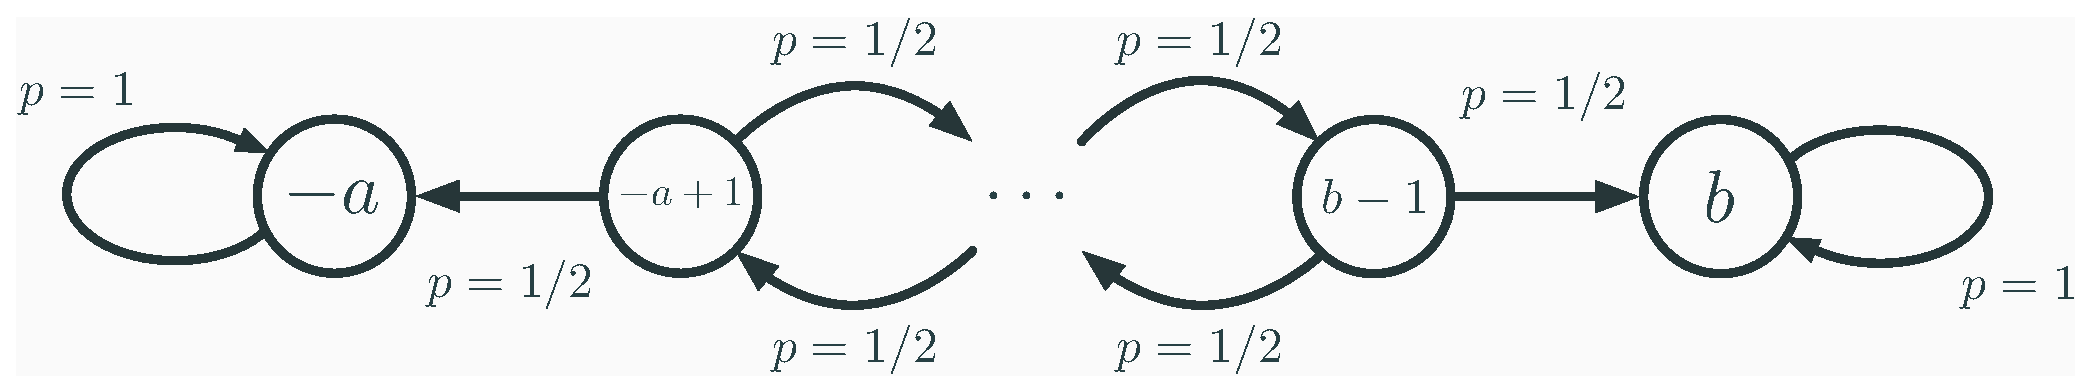
\includegraphics[width=0.8\textwidth]{\pref/gampling.eps}
\end{figure}


{赌徒谬误}
\begin{itemize}
    \item $A$的累计收入$\{X_n\}_{n\geq 0}$形成了Markov链.
    \item 根据Markov性,未来双方的收入变化只取决于现在,而和过去运气无关.
    \item 赌徒谬误(gambler's fallacy):深陷赌局中的人会按照自己历史上的运气来评估自己未来的运气,认为过去运气差未来运气就会变好.
    \item ``风水轮流转''在一场公平对赌中是不正确的认知.
    \item 思考:如何评估赌局的公平性?
\end{itemize}


{多步转移概率}
\begin{itemize}
    \item 如果对赌是公平的,那么我们应该认为两个人每一轮的累计收入分布都是一样的,即
    \[\Pr(X_n=i|X_0=0)=\Pr(X_n=-i|X_0=0).\]
    \item 因此,我们需要能够计算多步转移的概率.
    \item 设$p_{ij}^{(k)}$表示从状态$i$用$k$步转移到状态$j$的概率.
    \item $k$步转移概率形成了一个矩阵$\P^{(k)}$.
    \item Kolmogorov-Chapman方程:
    \[\P^{(k+l)}=\P^{(k)}\P^{(l)}.\]
\end{itemize}



{多步转移概率}
\begin{itemize}
    \item Kolmogorov-Chapman方程:
    \[\P^{(k+l)}=\P^{(k)}\P^{(l)}.\]
    \item 证明:由Markov性、时齐性和全概率公式,$
        p_{ij}^{(k+l)}=\Pr(X_{k+l}=j|X_0=i)=\sum_{\alpha}\Pr(X_{k+l}=j,X_k=\alpha|X_0=i)=\sum_{\alpha}\Pr(X_k=\alpha|X_0=i)\Pr(X_{k+l}=j|X_k=\alpha)=\sum_{\alpha} p_{i\alpha}^{(k)}p_{\alpha j}^{(l)}$.
    \item 特例:前向方程(forward equation)$\P^{(k+1)}=\P^{(k)}\P$,后向方程(backward equation)$\P^{(l+1)}=\P\P^{(l)}$.
    \item 推论:$\P^{(k)}=\P^k$.
    \item 若已知初始分布向量为$\lambda$,我们可以计算它随时间的演化:
		\[\lambda^\t,\lambda^\t \P,\dots,\lambda^\t \P^n,\dots\] %HW: 证明这个演化
\end{itemize}


{多步转移概率}
\centering
\begin{minipage}[t]{0.4\textwidth}
前向方程(往前一步):
    \centering
    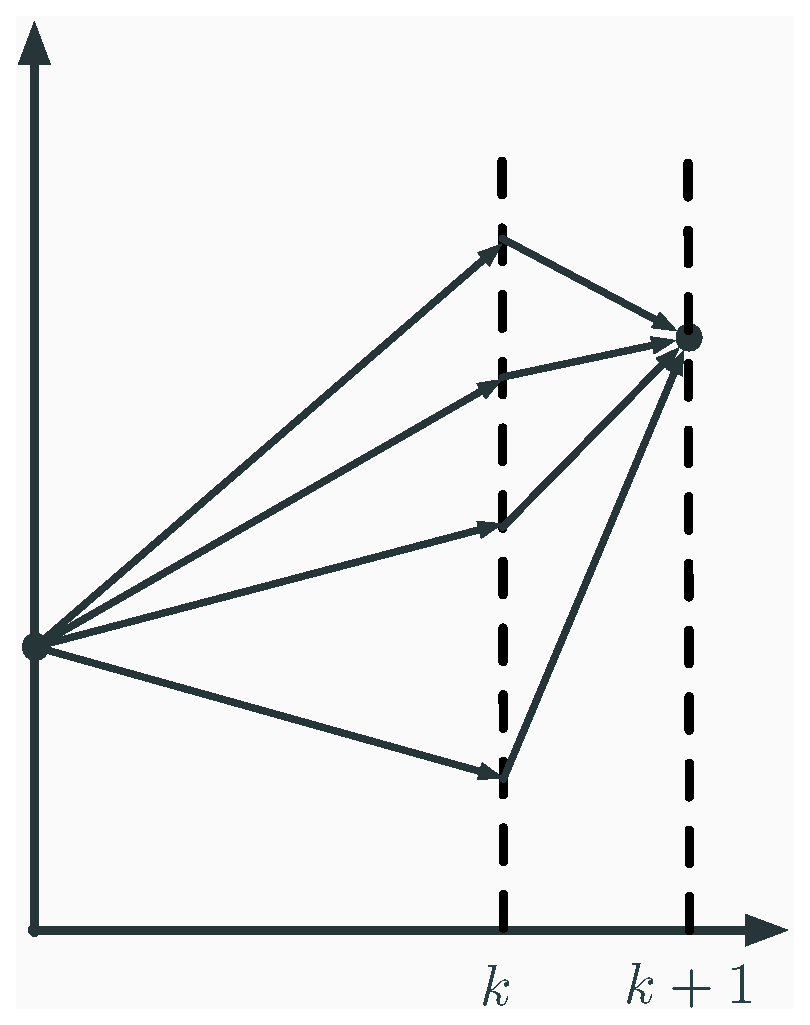
\includegraphics[width=0.6\textwidth]{\pref/forward-equation.eps}
\end{minipage}
\begin{minipage}[t]{0.4\textwidth}
后向方程(往回一步):
    \centering
    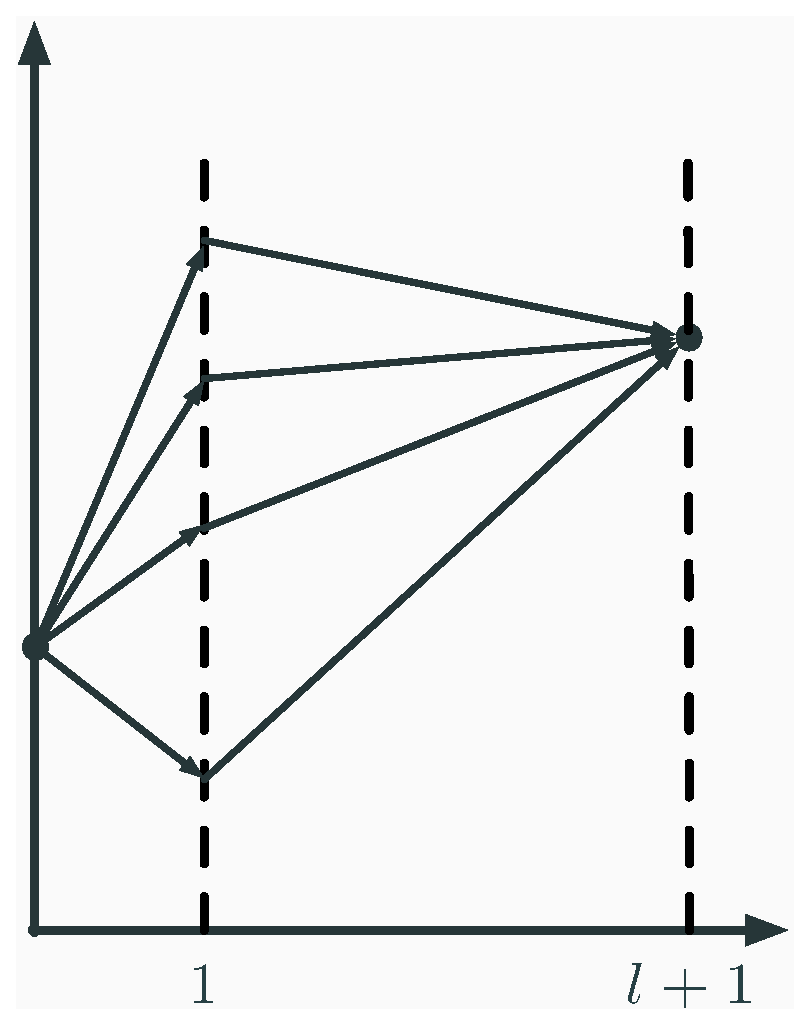
\includegraphics[width=0.6\textwidth]{\pref/backward-equation.eps}
\end{minipage}


{遍历定理与平稳分布}
\begin{itemize}
	\item 思考:如何计算公平对赌中$X_n$的概率分布?
	\item 我们先来看一个简单的例子. 假设$|p_{00}+p_{11}-1|<1$,考虑只有两个状态$0,1$,转移矩阵为
	\[\P=\begin{pmatrix}p_{00}&p_{01}\\p_{10}&p_{11}
	\end{pmatrix}.\]
\end{itemize}
\begin{figure}
    \centering
    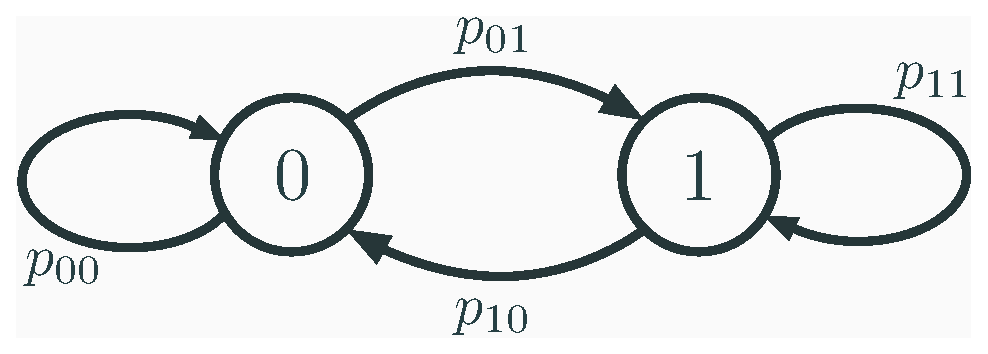
\includegraphics[width=0.4\textwidth]{\pref/simple-example.eps}
\end{figure}


{遍历定理}
\begin{itemize}
	\item 可以归纳证明:
	\begin{align*}
	    \P^n=&\frac{1}{2-p_{00}-p_{11}}\begin{pmatrix}1-p_{11}&1-p_{00}\\1-p_{11}&1-p_{00}\end{pmatrix}\\
	    &+\frac{(p_{00}+p_{11}-1)^n}{2-p_{00}-p_{11}}\begin{pmatrix}1-p_{00}&-(1-p_{00})\\-(1-p_{11})&1-p_{11}\end{pmatrix}.
	\end{align*}
	\item $\lim_{n\to\infty}p_{i0}^{(n)}=(1-p_{11})/(2-p_{00}-p_{11})$,$\lim_{n\to\infty}p_{i1}^{(n)}=(1-p_{00})/(2-p_{00}-p_{11})$.
	\item 随着时间的推移,Markov链初始状态对概率分布的影响逐渐消失. 这个规律具有普遍性,这就是遍历定理.
\end{itemize}


{遍历定理}
\begin{theorem}[遍历定理,Ergodic theorem]
Markov链的状态空间为$\MS=\{1,\dots,N\}$,转移矩阵为$\P=(p_{ij})$.
\begin{itemize}
    \item 如果对于某一个$n_0$有
    \begin{equation}
        \min_{ij}p_{ij}^{(n_0)}>0,\label{eq:reachable}
    \end{equation}
    那么存在分布$\lambda=(\lambda_1,\dots,\lambda_N)$使得
    \begin{equation}
        \lambda_i>0,\quad\sum_i\lambda_i=1,\label{eq:positive-distribution}
    \end{equation}
    并且对于每一个$j\in\MS$和任意$i\in\MS$都有
    \begin{equation}
    p_{ij}^{(n)}\to\lambda_j,n\to\infty.\label{eq:converge-to-limit}
    \end{equation}
\end{itemize}
\end{theorem}


{遍历定理}
\begin{theorem}[遍历定理,续]
\begin{itemize}
    \item 反之,如果存在满足 \eqref{eq:positive-distribution} 和 \eqref{eq:converge-to-limit} 的$\lambda$,则存在满足 \eqref{eq:reachable} 的$n_0$.
    \item 式 \eqref{eq:positive-distribution} 的$\lambda$满足
    \begin{equation}
        \lambda^\t = \lambda^\t\P.\label{eq:stationary}
    \end{equation}
\end{itemize}
\end{theorem}
\begin{itemize}
    \item 条件 \eqref{eq:reachable} 表明超过某个步数$n_0$之后,从$i$出发到达$j$的概率总是正的,这个条件被称为\emph{遍历}(ergodic).
    \item 条件 \eqref{eq:positive-distribution} 表明每一个状态被访问到的概率都是正的,没有``死状态''.
    \item 遍历定理表明遍历的Markov链从任何状态出发都是不可逆的,最终会把每个状态都走过一遍(遍历),变成一个混合均匀的状态.
    \begin{itemize}
        \item 这可以用来解释物理学中的扩散现象. % HW: 算一下Ehrenfest模型
    \end{itemize}
\end{itemize}


{平稳分布}
\begin{itemize}
    \item 满足条件 \eqref{eq:stationary} 的分布被称为\emph{平稳分布}(stationary distribution).
    \item 平稳分布为初始状态时,Markov链的演化与时间无关:$(X_k,\dots,X_{k+l})$的联合分布不依赖于$k$.
    \item 如果Markov链是遍历的,那么平稳分布是唯一的.
    \begin{itemize}
        \item 假设$\mu$是另外一个平稳分布,那么$\mu_j=\sum_\alpha\mu_\alpha p_{\alpha j}=\dots=\sum_{\alpha}\mu_\alpha p_{\alpha j}^{(n)}$.
        \item 因为$p_{\alpha j}^{(n)}\to \lambda_j$,所以$\mu_j=\sum_{\alpha} (\mu_\alpha\lambda_j)=\lambda_j$.
    \end{itemize}
    \item 非遍历Markov链也可能存在(唯一)平稳分布,考虑$\P=\begin{pmatrix}0&1\\1&0\end{pmatrix}$和$\lambda=(1/2,1/2)^\t$.
\end{itemize}


\section{Markov奖励过程(MRP)}
{决策理论}
\begin{itemize}
    \item 我们接下来的目标就是在Markov链上建立决策理论.
    \item 每一阶段我们可以选择某个行动,这个行动在Markov链会产生一些奖励.
    \item 我们的目标是选择恰当的行动方式是的我们的总奖励最大.
    \item 首先我们定义奖励的过程.
\end{itemize}

{Markov奖励过程}
\begin{itemize}
\item 一个\emph{Markov奖励过程}(Markov reward process,MRP)是四元组$\langle\MS,\P,\mathcal R,\gamma\rangle$:
\begin{itemize}
    \item $\MS$是一个有穷的状态集合.
    \item $\P$是一个状态转移矩阵,从$i$转移到$j$的概率记为$\P_{i,j}$.
    \item $\mathcal R$是一个奖励函数,$\mathcal R_s = \E[\textcolor{red}{R_{t+1}}|S_t=s]$:当$t$时刻位于状态$s$时 下一时刻(离开)获得的奖励的期望,$\textcolor{red}{R_{t+1}}$是下一阶段所处状态的奖励.
    \item $\gamma$是一个折扣系数,$\gamma\in[0,1]$.
\end{itemize}
    \item 注:条件数学期望$\E[\cdot|S_t=s]$可以理解为条件在$\{S_t=s\}$下定义的概率所求的期望.
\end{itemize}


{例子:学生MRP}
\begin{figure}
    \centering
    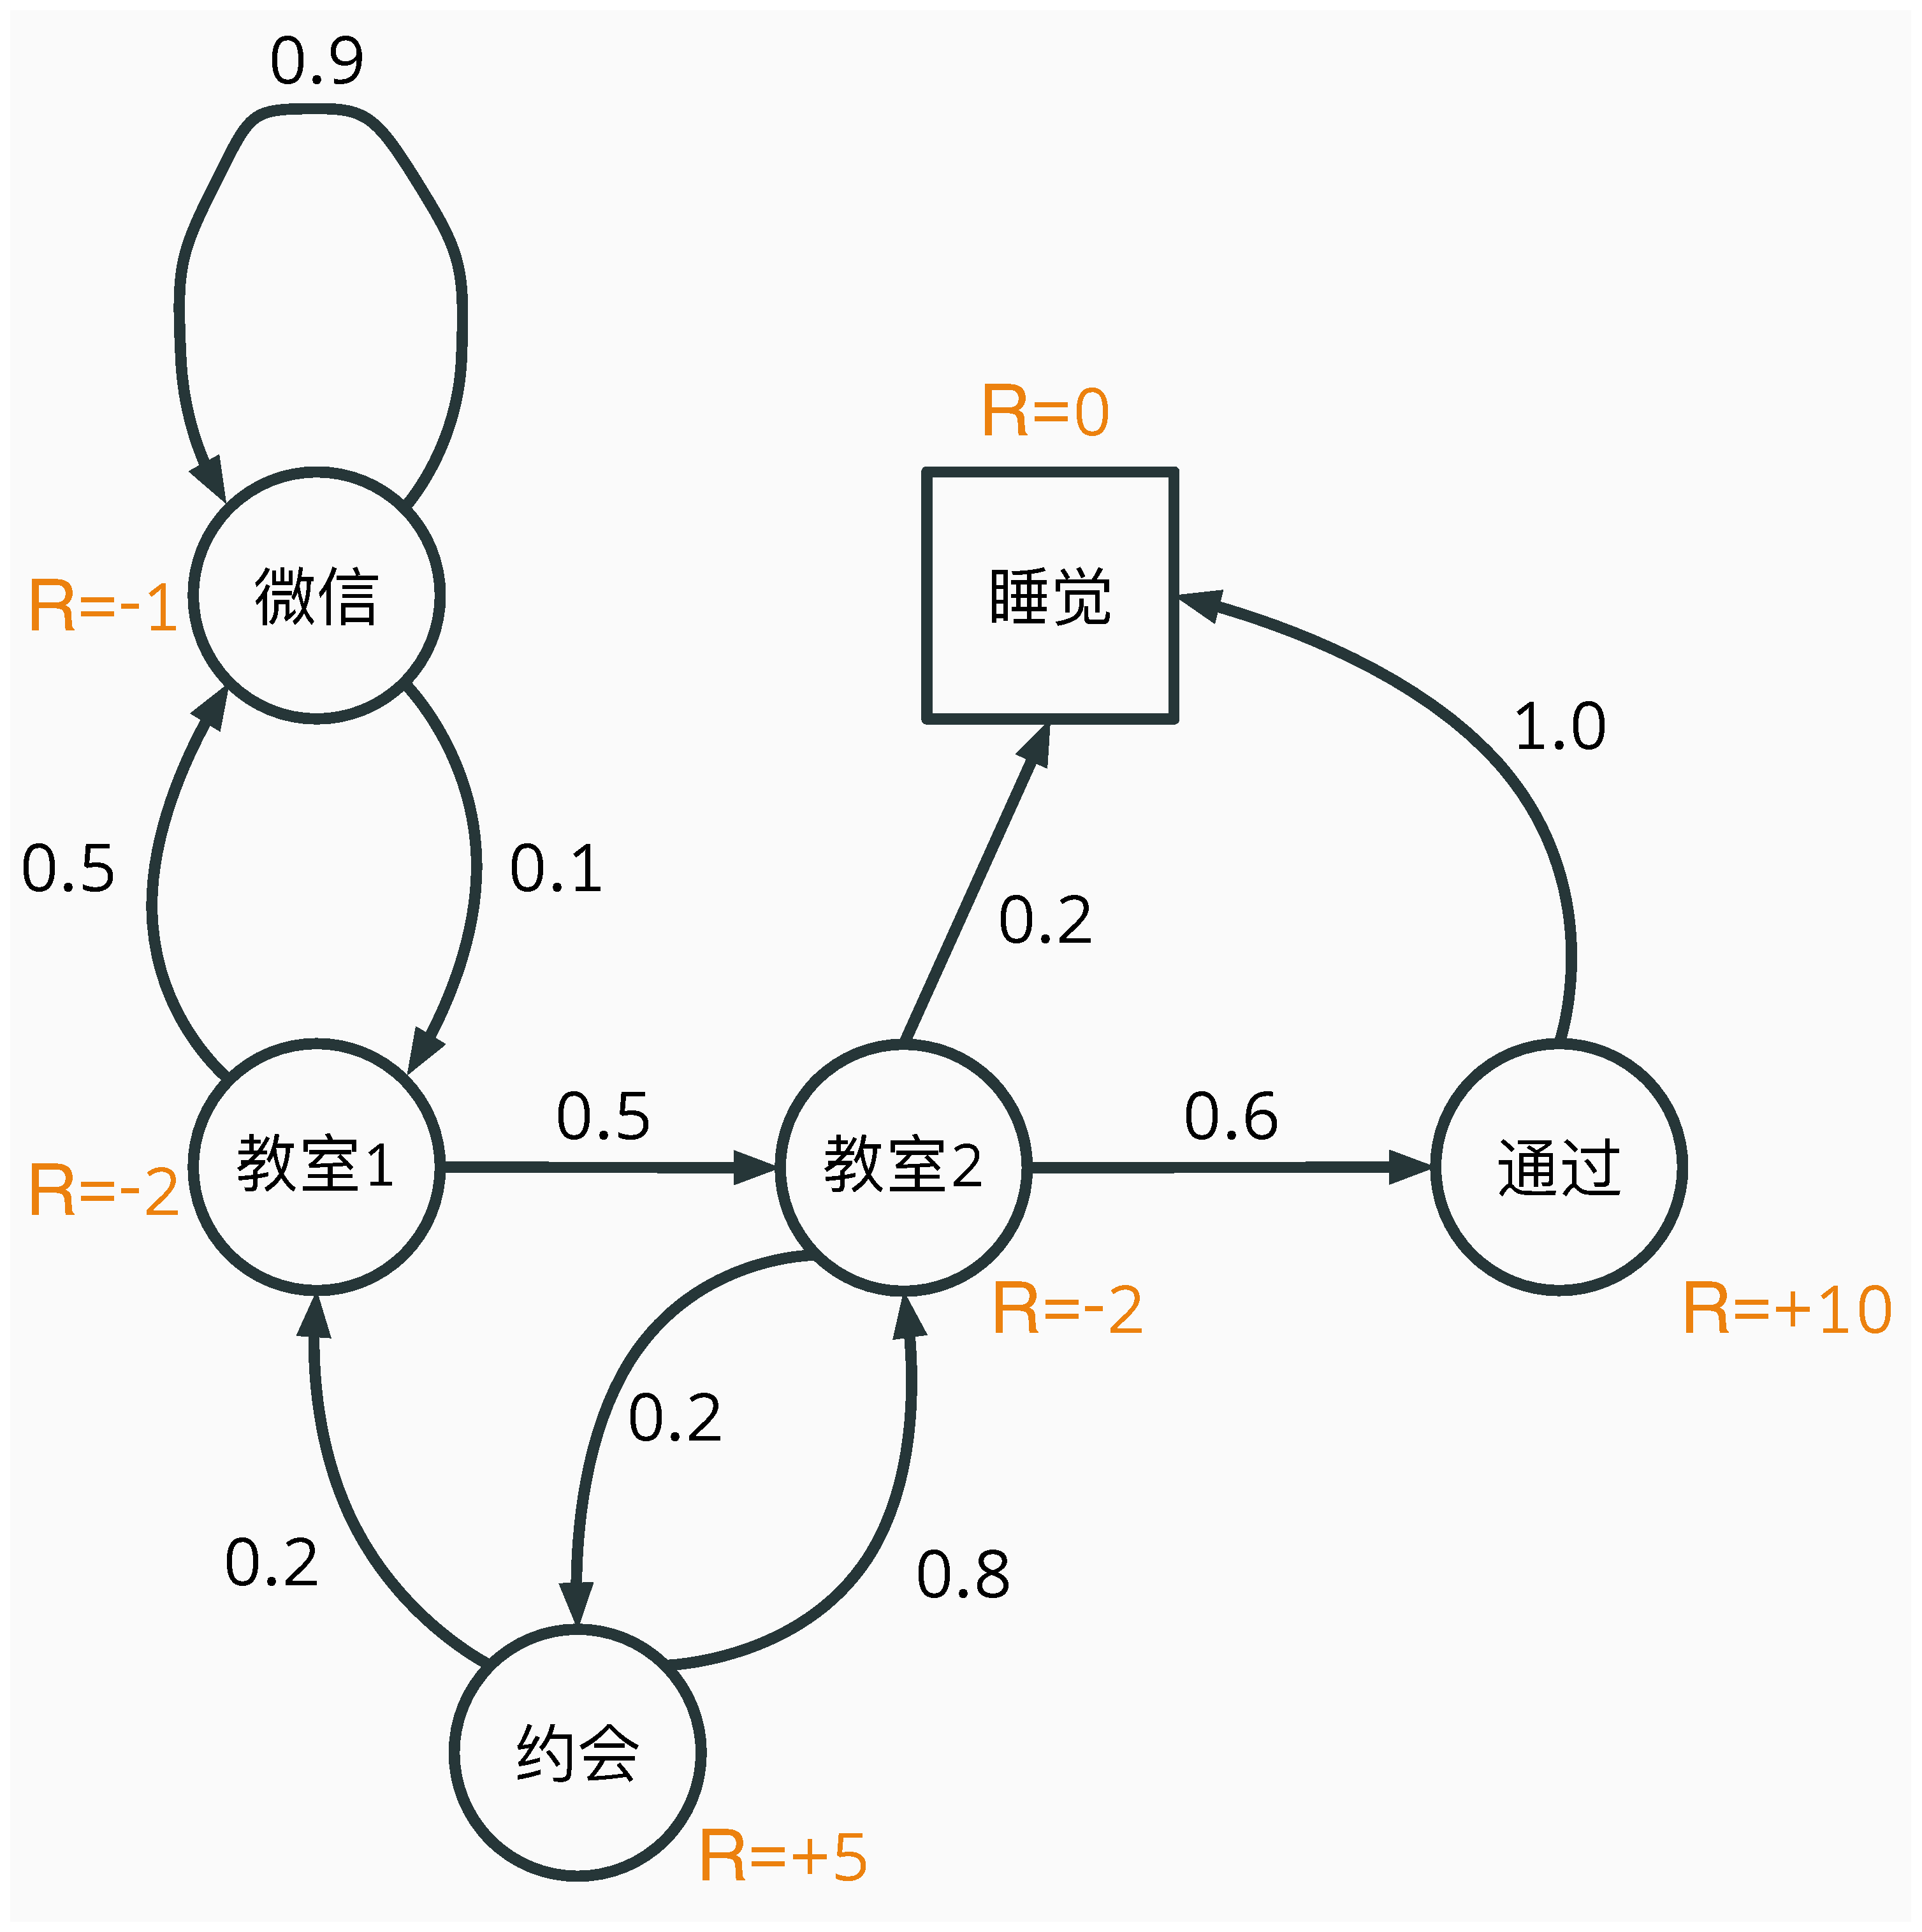
\includegraphics[height=0.8\textheight]{\pref/STR.eps}
\end{figure}


{回报}
\begin{itemize}
    \item MRP中,$t$时刻以后的总\emph{回报}(Return)$G_t$定义为
    \[G_t = R_{t+1}+\gamma R_{t+2} +\dots =\sum_{k=0}^\infty \gamma^kR_{t+k+1}.\]
        \item $\gamma \in[0,1]$衡量了未来下一时段1的奖励在当前时刻的价值.
        \item 未来$k+1$时刻的奖励对当前时刻$t$的作用是$\gamma^k R_{t+k+1}$.
        \item 若$\gamma\to0$,表示对奖励进行“短视”的评估;反之更“远见”.
\end{itemize}


{折扣系数的意义}
\begin{itemize}
    \item 许多MRP和后面学习的MDP都有与时间无关的折扣系数$\gamma <1$,原因:
\begin{itemize}
    \item 起始于对未来不确定性对冲:直接对应于利润率. 
    %具有不确定性,因此未来的回报更有风险,需要一个折扣风险的系数.
    %\item 数学上表示不麻烦.
    \item 动物和人类对即时回报具有偏好.
\end{itemize}
\item 有时也使用非折扣化的MRP(即$\gamma=1$),例如当所有的转移序列都会有固定的终止时间.
\end{itemize}


{价值函数}
\begin{itemize}
    \item 在MRP中,状态\emph{价值函数}(value function)$v(s)$表示从状态$s$出发的期望回报
    \[v(s) = \E(G_t|S_t=s).\]
    \item 价值函数$v(s)$衡量了状态$s$的长期效益.
    \item Markov性:只从当前起考虑未来收益,不考虑历史收益(沉没成本)的影响.
    \item 时齐性:价值函数的定义不依赖于时刻$t$
    (无穷阶段情形).
\end{itemize}



{MRP的Bellman方程}
\begin{itemize}
    \item 价值函数可以被分解为两部分:
\begin{itemize}
    \item 即时回报$\textcolor{red}{R_{t+1}}$
    \item 下一个状态开始的折扣价值 $\textcolor{green}{\gamma v(S_{t+1})}$
\end{itemize}
        \begin{align*}
        v(s) &= \E(G_t|S_t=s) \\
            &= \E(R_{t+1}+ \gamma R_{t+2} + \gamma^2 R_{t+3}+\dots | S_t= s) \\
            &= \E(R_{t+1} + \gamma (R_{t+2}+\gamma R_{t+3}+\dots) | S_t = s) \\
            &= \E(R_{t+1} + \gamma G_{t+1} | S_t = s) \\
            &= \E(\textcolor{red}{R_{t+1}} + \textcolor{green}{\gamma v(S_{t+1})}| S_t=s)\\
            &= {\textcolor{red}{\mathcal R_s} + \textcolor{green}{\gamma \sum_{s'\in \MS}\P_{s,s'}v(s')}}. % HW: 做一下破产博弈的Wald等式. 看一下zfx应随教材1.10三(100页),可以在题目里直接假设停时概率1有限
    \end{align*}
\end{itemize}


{矩阵形式的Bellman方程}
\begin{itemize}
    \item Bellman方程可以用矩阵形式表达:
        \[v = \mathcal R + \gamma \mathcal P v.\]
    这里$v$是列向量$v=(v(s))_{s\in\MS}$.
\end{itemize}


{Bellman方程的解}
\begin{itemize}
    \item Bellman方程是一个线性方程,可以被直接解:
    \[
        v =\mathcal R + \gamma \P v \implies (I-\gamma \P)v = \mathcal R \implies v = (I-\gamma \P)^{-1} \mathcal R.
   \]
    \item 对于$n$个状态的Markov链,计算复杂度为$\O(n^3)$.
    \item 对于较小的MRP可以直接解,太大的MRP开销太大.
    \item 对于大型MRP,可以采用迭代算法,例如:
    \begin{itemize}
        \item 动态规划(dynamic programming)
        \item Monte-Carlo评估(Monte-Carlo evaluation) 
        \item 时序差分学习(temporal-difference learning)
    \end{itemize}
\end{itemize}


\section{Markov决策过程(MDP)}
{Markov决策过程}
\begin{itemize}
    \item \emph{Markov决策过程}(Markov decision process)是一个定义了决策的MRP. 它可以看做一个任意状态都具有Markov性的\emph{环境}.
    \item 一个MDP是五元组$\langle\MS, \textcolor{green}{\mathcal A}, \P, \mathcal R, \gamma\rangle$.
        \begin{itemize}
            \item $\MS$是一个有限的状态集合.
            \item $\textcolor{green}{\mathcal A}$是一个有限的\emph{行动}(action)集合.
            \item $\P$是状态转移概率矩阵,
            \[\P_{ss'}^{\textcolor{green}{a}} = \Pr(S_{t+1} = s' | S_t = s, A_t = \textcolor{green}{a}).\]
            \item $\mathcal R$是一个奖励函数,$\mathcal R_s^{\textcolor{green}{a}} = \E(\textcolor{red}{R_{t+1}} | S_t = s, A_t = \textcolor{green}{a})$,$\textcolor{red}{R_{t+1}}$是进行某一行动到达某一状态后的奖励.
            \item $\gamma$是一个折扣系数$\gamma\in[0,1]$.
        \end{itemize}
    \end{itemize}


{例子:学生MDP}
\begin{figure}
    \centering
    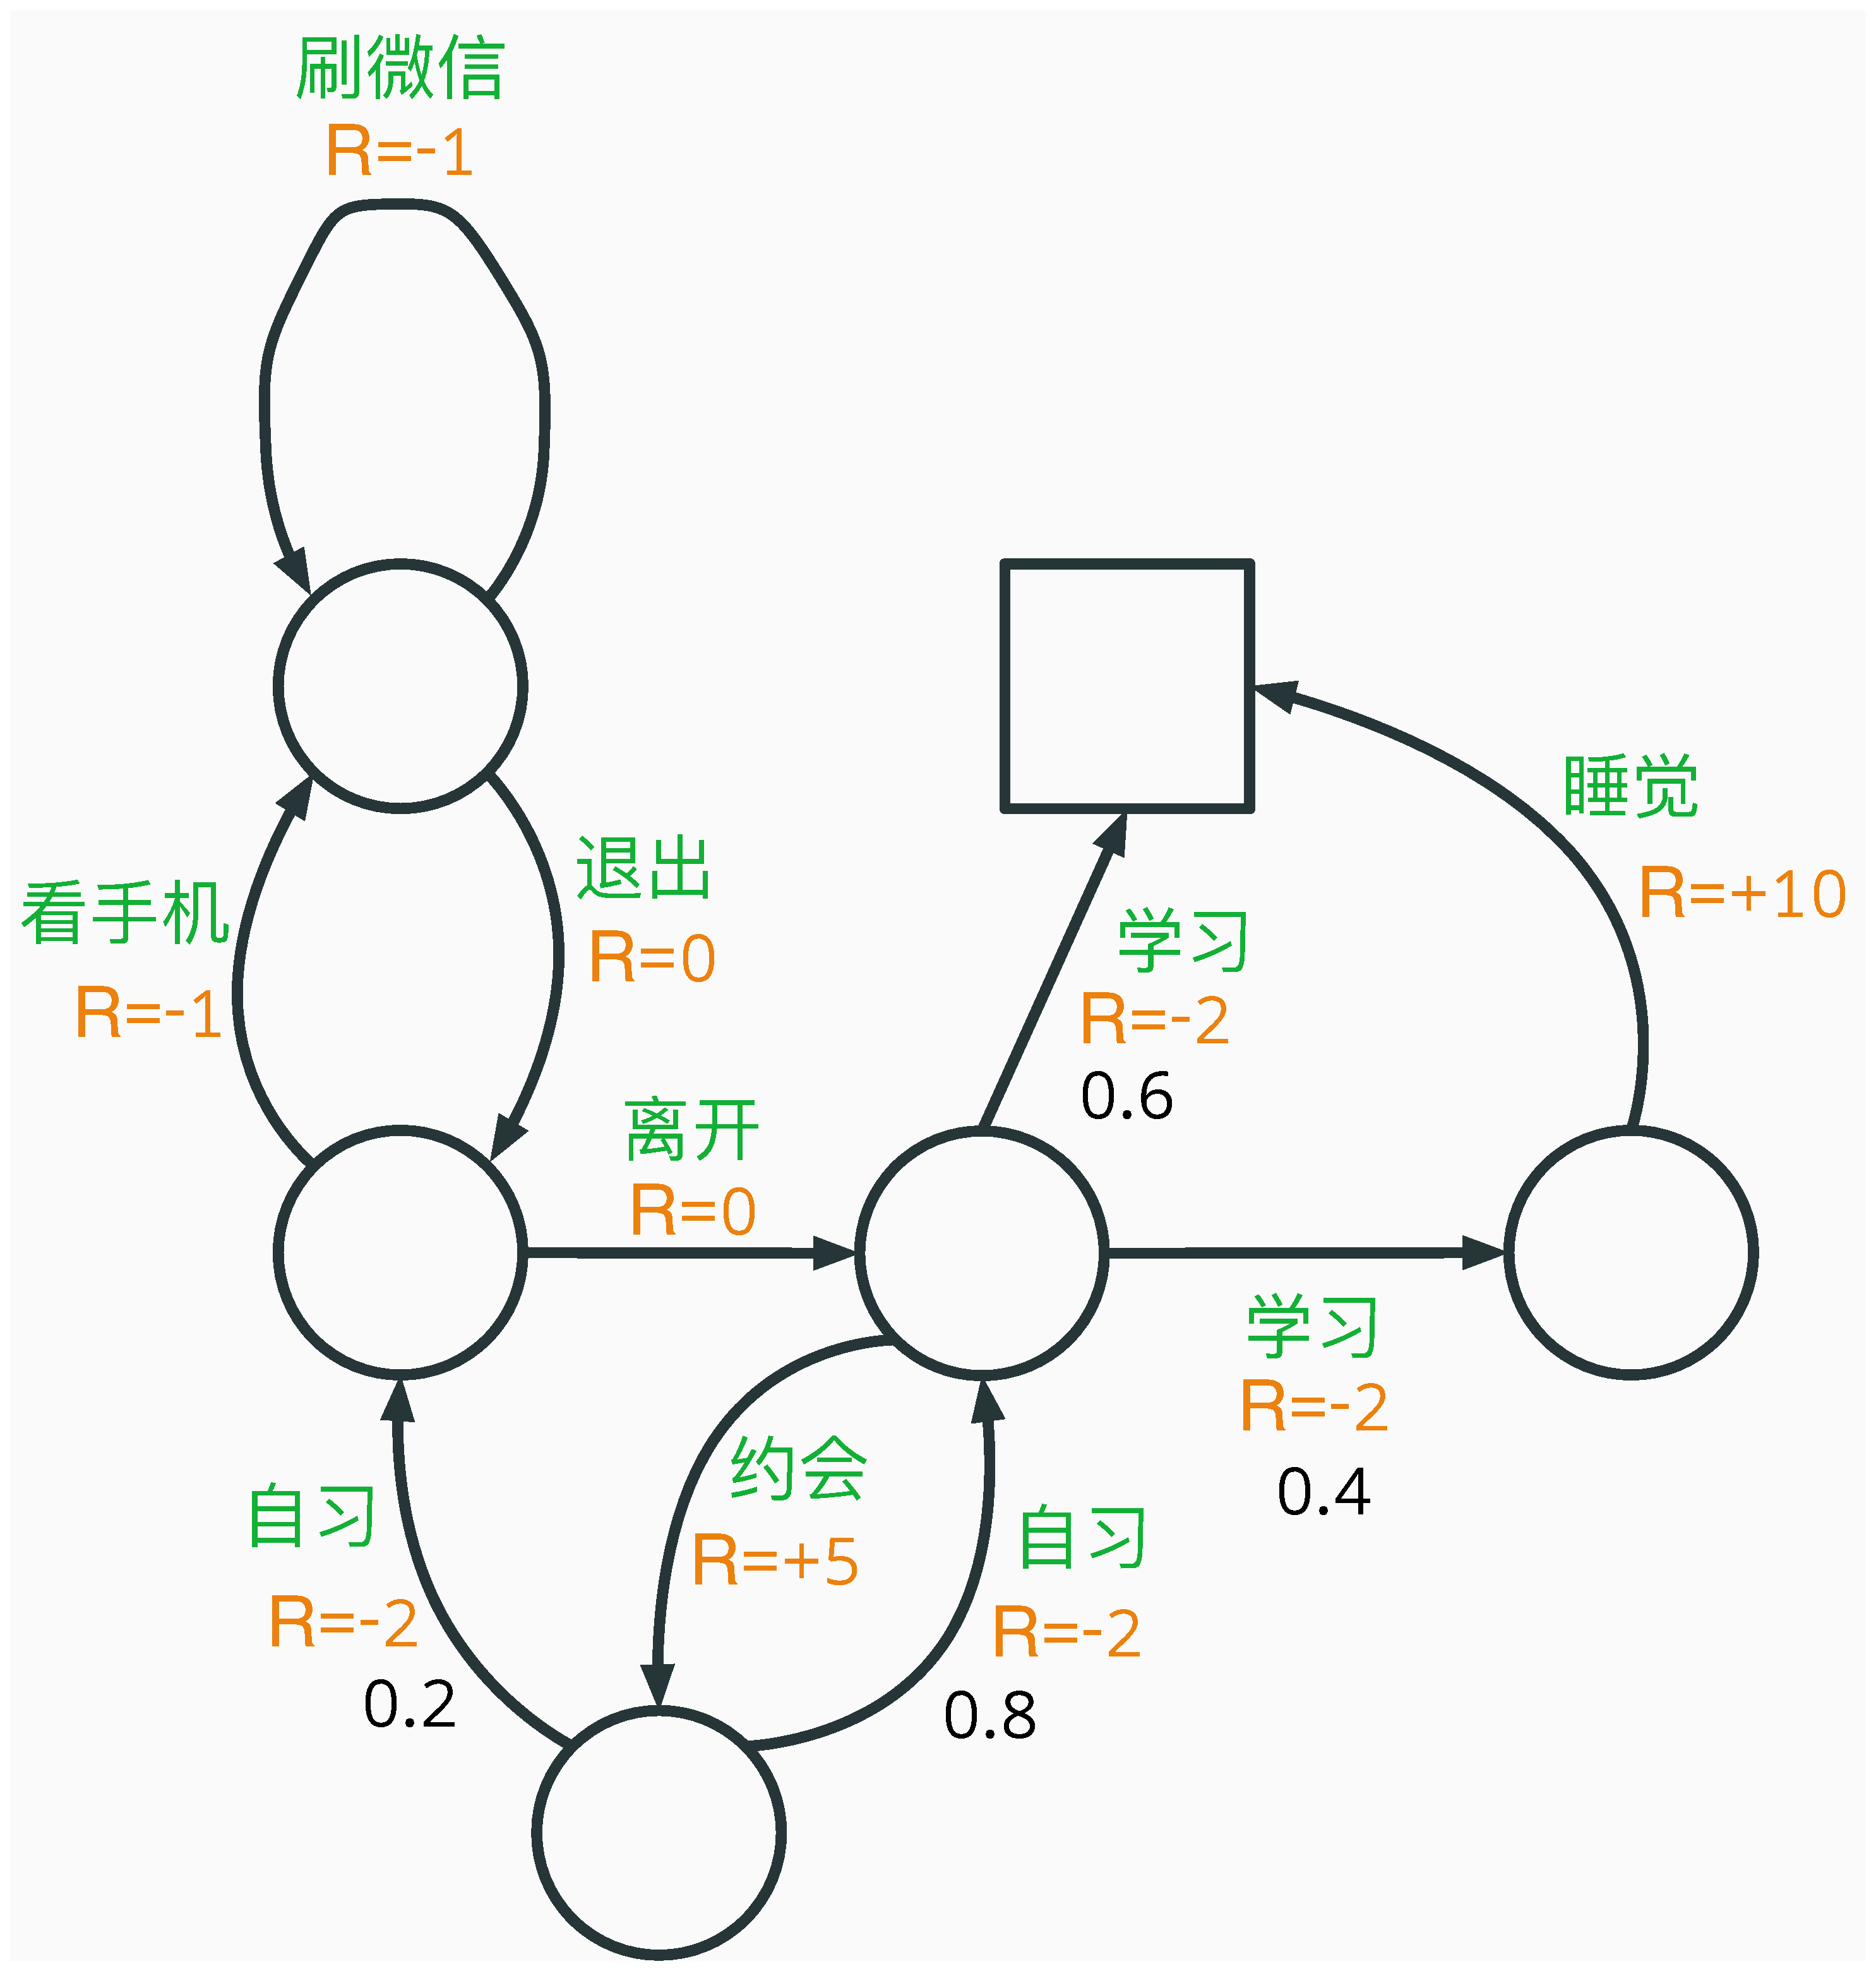
\includegraphics[height=0.8\textheight]{\pref/STD.eps}
\end{figure}


{策略}
\begin{itemize}
    \item     一个\emph{策略}(policy)$\pi$是给定状态下行动的分布,
    \[\pi(a|s) = \Pr(A_t=a | S_t = s).\]
    \item 一个策略完全决定了一个智能体在MDP环境中的行为.
    \item Markov性:MDP的策略取决于当前状态,而非历史状态.
    \item 时齐性:MDP的策略不依赖于时刻$t$.
\end{itemize}


{策略}
\begin{itemize}
    \item 给定一个MDP $\M=\langle\MS,\mathcal A,\P,\mathcal R, \gamma\rangle$和一个策略$\pi$.
    \item $\langle \MS, \P^{\pi}\rangle$是一个Markov链.
    \item $\langle\MS,\P^{\pi}, \mathcal R^{\pi}, \gamma\rangle$是一个MRP.
    \item 其中
\end{itemize}
\[\P_{s,s'}^{\pi} = \E_{a\sim\pi(\cdot|s)}(\P^a_{s,s'})=\sum_{a\in \mathcal A}\pi(a|s)\mathcal P_{s,s'}^{a},\]
    \[\mathcal R_s^{\pi} =\E_{a\sim\pi(\cdot|s)}(\mathcal R^a_s)=\sum_{a\in\mathcal A}\pi(a|s)\mathcal R_s^a.\]


{价值函数}
\begin{itemize}
    \item 在MDP中,状态-价值函数$v_\pi(s)$是从状态$s$出发,遵从策略$\pi$的期望回报
    \[v_\pi(s) = \E_\pi(G_t|S_t=s).\]
    \item     行动-价值函数$q_\pi(s,a)$是从状态$s$出发,采取行动$a$,遵从策略$\pi$的期望回报
    \[q_\pi(s,a) = \E_\pi(G_t|S_t=s,A_t=a).\]
    \item 注意,以上定义都具有Markov性和时齐性.
\end{itemize}


{Bellman期望方程}
\begin{itemize}
    \item 状态-价值函数可以被分解为:即时回报 加 后续状态的折扣价值,
\[v_\pi(s) = \E_\pi(R_{t+1} + \gamma v_\pi(S_{t+1})|S_t=s).\]
\item 行动-价值函数可以被类似地分解,
\[q_\pi(s,a) = \E_\pi(R_{t+1} + \gamma q_\pi(S_{t+1},A_{t+1})|S_t=s,A_t=a).\]
\item 二者之间的关系(全概率公式、一步转移概率):
\[q_\pi(s,a) =\mathcal R_s^a + \gamma \sum_{s'\in \MS}P_{s,s'}^a v_\pi(s').\]
\[v_\pi(s) = \E_{a\sim\pi(\cdot|s)}(q_\pi(s,a))=\sum_{a\in\mathcal A}\pi(a|s)q_\pi(s,a),\]
\end{itemize}


{Bellman期望方程}
\begin{itemize}
    \item 因此,我们得到MDP的Bellman期望方程:
\[v_\pi(s) = \sum_{a\in \mathcal A}\pi(a|s)\left(\mathcal R_s^a + \gamma \sum_{s'\in \MS}\P_{s,s'}^av_\pi(s')\right),\]
\[q_\pi(s,a) = \mathcal R_s^a + \gamma \sum_{s'\in \MS}\P_{s,s'}^a \sum_{a'\in \mathcal A}\pi(a'|s')q_\pi(s',a').\]
\item 矩阵形式:
\[v_\pi = \mathcal R^\pi + \gamma \P^\pi v_\pi = (I-\gamma \mathcal P^\pi)^{-1}\mathcal R^\pi.\]
\end{itemize}


{最优价值函数}
\begin{itemize}
    \item \emph{最优状态-价值函数} $v_\star(s)$ 是所有决策中最大的状态-价值函数
    \[v_\star(s) = \max_\pi v_\pi(s).\]
    \item \emph{最优行动-价值函数} $q_\star(s,a)$是所有决策中最大的行动-价值函数
    \[q_\star(s,a) = \max_\pi q_\pi(s,a).\]
    \item 最优价值函数确定了MDP中的最佳收益.
    \item 解MDP即确定达到最优价值函数的策略.
\end{itemize}


{最优策略}
\begin{itemize}
    \item 然而,每个状态取到最大价值的策略$\pi$可能并不是同一个.
    \item 幸运的是,确实存在一个这样的最优策略. 定义一个策略的偏序:
    \[\pi\ge\pi' \iff \forall s\in\MS\ v_\pi(s) \ge v_{\pi'}(s).\]
\end{itemize}
\begin{theorem}[MDP解的存在性]
对任意MDP,
\begin{itemize}
    \item 存在一个最优策略 $\pi_\star$使得$\forall \pi\ \pi_\star\ge\pi$.
    \item 最优策略取得最优状态-价值函数:$v_{\pi_\star}(s) = v_\star(s)$.
    \item 最优策略取得最优行动-价值函数:$q_{\pi_\star}(s,a)=q_\star(s,a)$.
\end{itemize}
\end{theorem}


{寻找最优决策}
\begin{itemize}
    \item 可以通过最大化$q_\star(s,a)$来寻找:
    \begin{itemize}
        \item 固定$s$.
        \item 找到一个$a_\star$使得$q_\star(s,a_\star)=\max_{a}q_\star(s,a)$,令$\pi_\star(a_\star|s)=1$.
        \item 对$\forall a\neq a_\star$,$\pi_\star(a|s)=0$.
    \end{itemize}
    \item 证明:根据选法,$\pi_\star$取得最优行动-价值函数.
    \item 由$v_\pi(s) = \E_{a\sim\pi(\cdot|s)}(q_\pi(s,a))\leq \E_{a\sim\pi(\cdot|s)}(q_\star(s,a))\leq q_\star(s,a_\star)=v_{\pi_\star}(s)$知$\pi_\star$取得最优状态-价值函数.
    \item 推论:对任意MDP,总存在一个非随机的最优决策.
    \item 如果我们知道$q_\star(s,a)$,我们就能获得最优决策. % HW: 找一个简单一点的例子,让他们算一下最优策略
\end{itemize}


{Bellman最优性方程}
\begin{itemize}
    \item 最优价值函数由Bellman最优性方程联系:
\[v_\star(s) = \max_a q_\star(s,a),\]
\[q_\star(s,a) = \mathcal R_s^a + \gamma \sum_{s'\in \MS}\P_{s,s'}^av_\star(s'),\]
\[v_\star(s) = \max_a\left\{\mathcal R_s^a + \gamma \sum_{s'\in \MS}\P_{s,s'}^av_\star(s')\right\},\]
\[q_\star(s,a) = \mathcal R_s^a+\gamma \sum_{s'\in \MS}\P_{s,s'}^a\max_{a'}q_\star(s',a').\]
\end{itemize}


{解Bellman最优性方程}
    \begin{itemize}
        \item Bellman最优性方程不是线性的. 因此没有解析形式的(closed form)解.
        \item 但是MDP的数值解是可以多项式时间求出来的.
        \item 我们一般采用迭代算法求解:
        \begin{itemize}
            \item 价值迭代(value iteration)
            \item 策略迭代(policy iteration)
            \item Q-learning
            \item Sarsa
        \end{itemize}
    \end{itemize}

{关于Bellman方程}
\begin{itemize}
    \item Bellman方程是强化学习(reinforcement learning)、经济学动态优化(dynamic optimization)的核心.
    \item Bellman方程的推导是Markov链中最为常用的技巧:考虑从当前状态转移到下一状态,利用全概率公式,一步转移会将两个状态之间的概率(期望)用递推公式联系起来.
    \begin{itemize}
        \item 随机过程中的例子:前向方程、Wald等式、调和函数(harmonic function).
        \item 后面的HMM也是类似的例子.
    \end{itemize}
\end{itemize}


\section{隐Markov模型(HMM)}

问题的引入

\begin{itemize}
    \item 我们考虑Markov链上的另一种应用.
    \item 在统计学和机器学习中,我们有时候要处理一类含时间的数据.
    \item 最简单的情况是回归,即数据完全由所处时刻决定.
    \item 但是通常,现在的数据依赖于过去的数据.
    \item 因此,一种最简单的考虑就是数据依赖于Markov链,这就是隐Markov模型.
\end{itemize}


{隐Markov模型}
\begin{itemize}
    \item 一个\emph{隐Markov模型}(hidden Markov model,HMM)是一列随机变量$X_1,X_2,\dots, X_t$,满足:
    \begin{itemize}
        \item $X_t$的分布仅依赖于隐状态$Z_t$,即$\Pr(X_1,\dots,X_t|Z_1,Z_2,\dots,Z_t)=\prod_i \Pr(X_i|Z_i)$.
        \item $\{Z_t\}$构成一条Markov链.
    \end{itemize}
\end{itemize}
\begin{figure}
    \centering
    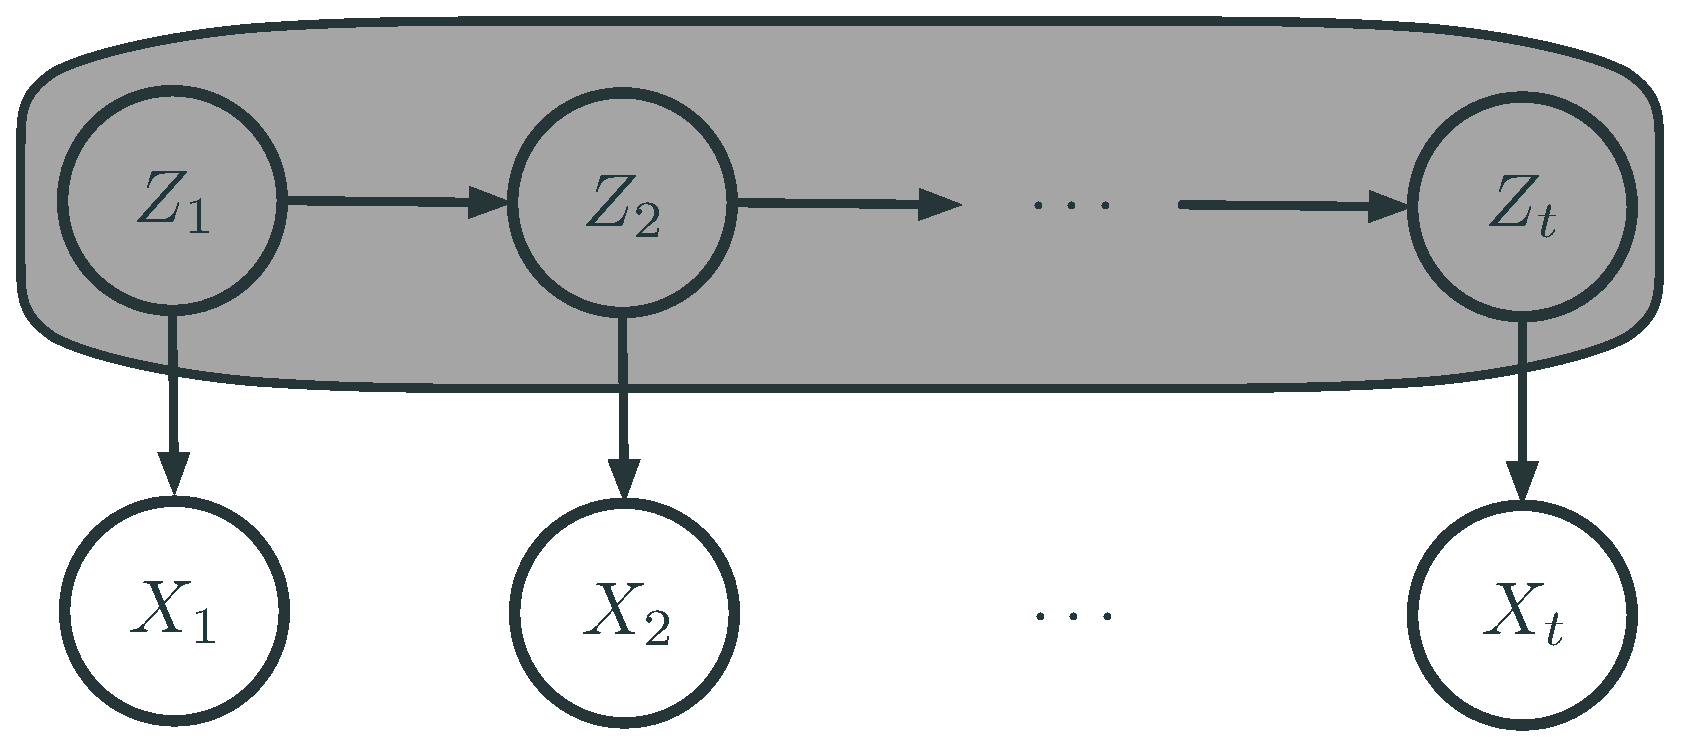
\includegraphics[width=0.6\textwidth]{\pref/HMM.eps}
\end{figure}


{有限观测HMM}
\begin{itemize}
    \item 一个HMM包含:
    \begin{itemize}
        \item $\mathcal Z$
        : 有限的状态集合.
        \item $\mathcal X$: 有限的观测集合.
        \item $T: \mathcal Z\times\mathcal Z\to \R_{\geq 0}$,$\mathcal Z$的转移概率.
        \item $M:\mathcal Z\times \mathcal X\to \R_{\geq 0}$,给定状态时的观测概率(条件概率).
        \item $\lambda:\mathcal Z\to\R_{\geq 0}$,初始状态的先验概率分布列.
    \end{itemize}
    \item 如果随机过程$\{X_t\}$的值域是有限集,我们则可以用矩阵表达HMM.
    \begin{itemize}
    \item $T$是$\{Z_t\}$的转移矩阵.
    \item $M$是观测矩阵:$M_{i,k} = \Pr(X_t=k|Z_t=i)$.
    \item $\lambda$是一个概率向量.
    \end{itemize}
\end{itemize}


\subsection{评估问题}
{HMM的评估}
\begin{itemize}
   \item 给定一个特定的HMM,它对实际观测序列的拟合程度有多好?
   \item 记号:随机向量$X=(X_1,\dots,X_t)$,$Z=(Z_1,\dots,Z_t)$.
   \item  HMM的\emph{评估}(evaluation)问题:给定一个HMM $\M$,以及它的观测历史$x=(x_1,x_2,\dots,x_t)$,计算$\Pr(X=x|\M)$.
   \item 关键困难:我们不知道状态历史$Z=(z_1,z_2,\dots,z_t)$.
\end{itemize}


{朴素方法}
    \begin{itemize}
    \item 直接使用条件概 率进行推导:
    \[
        \Pr(X=x|\M) =\sum_{Z=(z_1, \dots, z_t) \in \mathcal Z} \Pr(X=x|Z=z, \M)\Pr(Z=z|\M),
    \]
    \[
        \Pr(X=x|Z=z,\M) = \prod_{i=1}^t \Pr(X_i = x_i| Z_i = z_i) = M_{z_1,x_1}\cdot M_{z_2,x_2}\dots M_{z_t,x_t},
    \]
    \begin{align*}
        \Pr(Z=z|\M) &= \Pr(Z_1 = z_1) \prod_{i=2}^t\Pr(Z_i = z_i| Z_{i-1} = z_{i-1}) 
        \\
        &= \lambda_{z_1}\cdot T_{z_1,z_2}\cdot T_{z_2,z_3}\dots T_{z_{t-1},z_t}.
    \end{align*}
    \item 时间复杂度: $\O(t|\mathcal Z|^t)$.
    \end{itemize}


{前向算法}
    \begin{itemize}
    \item 思路:类似前向方程,我们可以从前$k$步的结果推出前$k+1$步的结果. 因此可以列出递推方程.
    \item 记号:$X_{i:j}=(X_i,\dots,X_j)$.
    \item 具体地,定义$\alpha_k(z):= \Pr(X_{1:k}=x_{1:k}, Z_k=z| \M)$,我们有
    \begin{itemize}
        \item $\alpha_1(z) = \lambda(z)M_{z,x_1}$.
        \item $\alpha_{k+1}(z) = \sum_{z' \in \mathcal Z}\alpha_{k}(z')T_{z',z}M_{z,x_{k+1}}$.
    \end{itemize}
    \item $\Pr(X=x| \M) = \sum_{z\in \mathcal Z}\alpha_t(z)$.
    \item 时间复杂度 $\mathcal O(t|\mathcal Z|^2)$.
\end{itemize}



{后向算法}
   \begin{itemize}
    \item 类似后向方程,从前$k+1$步的结果推出前$k$步的结果. 同样可以列出递推方程.
    \item 定义$\beta_k(z):=\Pr(X_{k+1:t}=x_{k+1:t} | Z_k=z,\M)$,我们有
    \begin{itemize}
        \item 当$k = t$,$\beta_k(z) = 1$.
        \item 当$1 \le k < t$,$\beta_{k}(z) = \sum_{z' \in \mathcal Z}T_{z,z'}M_{z',x_{k+1}}\beta_{k+1}(z')$.
    \end{itemize}
    \item $\Pr(X=x| \M) = \sum_{z\in \mathcal Z}\lambda(z)M_{z,x_1}\beta_1(z)$.
    \item 时间复杂度 $O(t|\mathcal Z|^2)$.
\end{itemize}


\subsection{解释问题}
{HMM的解释问题}
    \begin{itemize}
    \item HMM的\emph{解释}(explanation)问题:给定一个 HMM $\M = (\mathcal Z, \mathcal X, T, M, \lambda)$, 一列观测历史$x = (x_1, x_2, \dots, x_t)$, 寻找一个状态序列,能最好地解释这些历史观察.
    \item 具体地,我们考虑如下四个问题
    \begin{enumerate}
        \item 过滤(filtering):计算$\Pr(Z_k = s|X_{1:k}=x_{1:k}, \M)$.
        \item 平滑(smoothing): 计算$\Pr(Z_k = s|X=x, \M)$,$k < t$.
        \item 预测(prediction): 计算$\Pr(Z_k = s|X=x, \M)$,$k > t$.
        \item 解码(decoding): 找到最有可能的状态序列 $z = (z_1, z_2, \dots, z_t)$.
    \end{enumerate}
\end{itemize}




{过滤:$\Pr(Z_k = s|X_{1:k}=x_{1:k}, \M)$}
\begin{itemize}
    \item 回顾:$\alpha_k(s)= \Pr(X_{1:k}=x_{1:k}, Z_k=s| \M)$. 
    \item 我们有
    \begin{align*}
        \Pr(Z_k = s|X_{1:k}=x_{1:k}, \M) & = \frac{\Pr(X_{1:k}=x_{1:k}, Z_k=s| \M)}{\Pr(X_{1:k}=x_{1:k}| \M)} \\
        &= \frac{\alpha_k(s)}{\sum_{z\in\mathcal Z}\alpha_k(z)}.
    \end{align*}
\end{itemize}


{平滑:$\Pr(Z_k = s|X=x, \M)$,$k < t$} 
\begin{itemize}
    \item 回顾:$\alpha_k(s)= \Pr(X_{1:k}=x_{1:k}, Z_k=s| \M)$.
    \item 回顾:$\beta_k(s)=\Pr(X_{k+1:t}=x_{k+1:t} |Z_k=s, \M)$.
    \item 可以证明:
        \[\Pr(z_k = s|X=x, \M)=\frac{\beta_k(s)\alpha_k(s)}{\sum_{z\in\mathcal Z}\alpha_t(z)}.
    \]% HW: 推导这个
    % \[\Pr(X_k = s|z, \M) =& \frac{\Pr(z_{1:k}, z_{k+1:t}, X_k=s| \M)}{\Pr(z| \M)} 
    %     \\
    %     =& \frac{\Pr(z_{k+1:t}| z_{1:k}, X_k=s,\M)\Pr(z_{1:k}, X_k=s| \M)}{\Pr(z| \M)}
    %     \\
    %     =& \frac{\Pr(z_{k+1:t}| X_k=s,\M)\Pr(z_{1:k}, X_k=s| \M)}{\Pr(z| \M)}
    %     \\
    %     =& \frac{\beta_k(s)\alpha_k(s)}{\Pr(z| \M)} = \frac{\beta_k(s)\alpha_k(s)}{\sum_{x\in\mathcal X}\alpha_t(x)} 
    % \]
\end{itemize}



{预测:$\Pr(Z_k = s|X=x, \M)$,$k > t$.}
\begin{itemize}
    \item 首先用过滤计算 $\lambda=\Pr(Z_t = s|X=x, \M)$.
    \item 然后用 $\lambda$ 作为Markov的初始状态,向前计算$k-t$步.
\end{itemize}


{*解码:Viterbi算法}
\begin{itemize}
    \item 定义 
    $$\delta_k(s) = \max_{Z_{1:k-1}}\Pr(Z_{1:k} = (z_{1:k-1}, s), X_{1:k}=x_{1:k}| \M).$$
    \item 根据一步转移,我们有
    $$\delta_{k+1}(s) = \max_{q\in \mathcal Z}\{\delta_k(q)T_{q,s}\}M_{s,x_{k+1}}.$$
    \item 问题转化为: 记录最高概率的路径,这是一个动态规划问题.
\end{itemize}


\newcommand{\pre}{\mathrm{Pre}}
{*解码: Viterbi算法}
\begin{itemize}
    \item 初始化:
    \begin{itemize}
        \item $\delta_1(s) = \lambda(s)M_{s,z_1}$.
        \item $\pre_1(s) = \varnothing$.
    \end{itemize}
    \item 对 $k=1, 2, \dots, t-1$,$s \in \mathcal Z$:
    \begin{itemize}
        \item $\delta_{k+1}(s) = \max_{q\in \mathcal Z}\{\delta_k(q)T_{q,s}\}M_{s,x_{k+1}}$.
        \item $\pre_{k+1}(s) = \argmax_{q\in \mathcal Z}\{\delta_k(q)T_{q,s}\}$.
    \end{itemize}
    \item $z_t = \argmax_{s \in \mathcal Z}\delta_{t}(s)$.
    \item 对 $1 \le k < t$,$z_k = \pre_{k+1}(z_{k+1})$.
    \item 时间复杂度: $\mathcal O(t|\mathcal Z|^2)$.
\end{itemize}

\endgroup

\part{信息与数据}\label{part:information-data}
\chapter{信息论基础}\label{chap:information-theory}
\begingroup
\newcommand{\pref}{Chapters/information-theory/figures}

信息是什么?不同于真实的物理世界,信息仿佛看不见,摸不着. 然而,任何人都可以体会到信息的存在,信息是我们认识世界的基础. 信息的存在正如同物理世界中的能量、动量一般,抽象而具有一般性. 信息论已经在计算机、AI、认知理论等诸多领域中得到了广泛的应用. 本章探讨信息论的基础,并给出他们在AI中的一些应用. 

在\Cref{sec:entropy},我们讨论熵的概念与性质. 在\Cref{sec:kl-divergence},我们讨论Kullback-Leibler散度的概念与性质. 在\Cref{sec:Shannon-thm-proofs},我们给出Shannon定理证明. 

\section{熵}\label{sec:entropy}


\subsection{概念的导出}

我们常说“恐惧来源于未知”,信息似乎代表着某种确定的东西,某种知识,因而和不确定性有相反的关系. 更精确地说,\emph{消除不确定性的东西被称为信息.} 当然,这句话本身似乎是一种循环论证,它并没有真正回答信息或者不确定性到底是什么. 所以我们进一步的问题是,给定一个“对象”,如何定量衡量它不确定性(或信息量)?

然而,单个对象的信息是一个非常难以划定的概念. 同样的内容,对于不同的人来说,信息量是完全不同的. 比如说,已经学过信息论的读者再看这一部分内容,他获得的信息一定比没有学过的读者要少得多. 因而实际上,一种更加容易的办法是我们将世界视为不确定的,因而有多种可能的对象,然后考虑这一堆对象的信息量. 比如说,这本书的读者的背景是不确定的,可能学过信息论,也可能没学过,但是我们可以综合考虑不同读者的背景,然后给出一个信息的概率分析. 

我们可以用数学来表述上面的考虑,假如我们进行一次试验,一共有$n$种可能的结果,第$i$种发生的概率为$p_i$. 我们预测试验的结果,如果越能正确地预测,那么就说明我们对这个试验中包含的信息知道的越多. 假如$p_1=1$,那么我们完全确定试验一定会产生结果$1$. 如果$p_i=1/n$,那么我们完全无法预计试验的结果. 我们对试验结果的预期与试验结果的概率分布有密切联系. 因此概率分布给我们带来了\textbf{信息}\index{信息},使得我们能够产生不同的判断. 另一方面,概率分布带来了\textbf{不确定性}\index{不确定性},使我们不能总是确信预言会成真. 

我们遵循“信息论之父”Shannon的思路,为信息提供一个严格的数学模型:熵. 假设随机变量$X$表示了所有可能的结果(编号为$1$到$n$),$\Pr(X=i)=p_i$,$p=(p_1,\dots,p_n)$,有时候也把$p_i$写作$p(i)$. 我们把不确定性度量记为$H(p)$. Shannon假设$H$满足以下三个性质:
\begin{enumerate}
    \item $H$是一个连续函数.
    \item 事件结局可能数变多则不确定性增大:$p_i=1/n$时,$H(p)$随$n$单调递增,$n$是正整数.
    \item 如果一个试验被分成了两个相继的试验,那么原来的$H$应该等于分开之后的$H$的加权和.
\end{enumerate}

\begin{remark}
    第三个假设可以用下图来理解. 
\begin{center}
\documentclass{standalone}
% font set
\usepackage{ctex}
\usepackage{fontspec}
\usepackage[T1]{fontenc}
\usepackage[sc]{mathpazo}
\usepackage{anyfontsize}
\setmainfont{Source Serif 4}
\setsansfont{Source Sans 3}
\setmonofont{Menlo}
\setCJKmainfont[BoldFont=黑体-简 中等,ItalicFont=楷体-简 常规体]{宋体-简 常规体}

% colors
\usepackage[dvipsnames]{xcolor}
\definecolor{pku-red}{RGB}{139,0,18}
\usepackage{colortbl}
\newcommand{\light}[1]{\textcolor{Orchid}{#1}}
\newcommand{\contrastlight}[1]{\textcolor{TealBlue}{#1}}

% plots
\usepackage{tikz}
\usepackage{tikz-cd}
\usetikzlibrary{arrows}
\usetikzlibrary{arrows.meta,positioning,calc,3d}
\usepackage{pgfplots}
\pgfplotsset{compat=newest}
\tikzset{
    punkt/.style={
        rectangle,
        rounded corners,
        draw=black, very thick,
        minimum height=2em,
        inner sep=6pt,
        text centered,
        fill=gray!30
    }
}

% math package
\let\Bbbk\relax
\usepackage{amsmath}
\usepackage{mathrsfs}
\usepackage{amssymb}
\usepackage{amsfonts}
\usepackage{stmaryrd}
\usepackage{latexsym}
\usepackage{extarrows}
\SetSymbolFont{stmry}{bold}{U}{stmry}{m}{n}
\begin{document}
\begin{tikzpicture} [
  level distance=2cm,
  grow'=right,
  level 1/.style= {sibling distance=0.8cm},
  solid node/.style= {circle,draw,inner sep=1.5,fill=black},
  edge from parent/.style={very thick,draw}
]
\node (0) [solid node] {}
  child {node (A1) [solid node,label=right: {$1$}] {} edge from parent node [above] {\scriptsize $1/2$}}
  child {node (A2) [solid node,label=right: {$2$}] {} edge from parent node [above right] {\scriptsize $1/3$}}
  child {node (A3) [solid node,label=right: {$3$}] {} edge from parent node [below] {\scriptsize $1/6$}};
\end{tikzpicture}
\qquad
\begin{tikzpicture} [
  level distance=1cm,
  grow'=right,
  level 1/.style= {sibling distance=1cm},
  level 2/.style= {sibling distance=0.8cm},
  solid node/.style= {circle,draw,inner sep=1.5,fill=black},
  edge from parent/.style={very thick,draw}
]
\node (0) [solid node] {}
  child {node (A1) [solid node,label=right: {}] {} 
  child {node (B1) [solid node,label=right: {$1$}] {} edge from parent node [above] {\scriptsize $1$}}
  edge from parent node [above]{\scriptsize $1/2$}
    }
  child {node (A2) [solid node,label=right: {}] {} 
  child {node (B2) [solid node,label=right: {$2$}] {} edge from parent node [above] {\scriptsize $2/3$}}
  child {node (B3) [solid node,label=right: {$3$}] {} edge from parent node [below] {\scriptsize $1/3$}}
  edge from parent node [below] {\scriptsize $1/2$}
  };
  
\end{tikzpicture}
\end{document}
\end{center}

    假设我们有一个试验,有三种可能的结果,$1,2,3$,概率分别为$1/2,1/3,1/6$. 该试验的不确定性是$H(1/2,1/3,1/6)$. 我们把试验分成两步相继的试验,第一步试验有两种可能的结果,概率分别都是$1/2$. 当第一步试验出现上面的结果时,第二步试验以概率$1$产生结果$1$;当第二步试验出现下面的结果时,第二步试验以概率$2/3$产生结果$2$,以概率$1/3$产生结果$3$. 我们可以看到,分成两步之后,第一步试验的不确定性是$H(1/2,1/2)$,第二步试验的不确定性有一半概率是$H(1)$(上面的分支),有一半概率是$H(2/3,1/3)$(下面的分支),因而加权的不确定性是$1/2\cdot 0+1/2\cdot H(2/3,1/3)$. 因此第三个假设可以具体表述为
\[
H\left(\frac{1}{2},\frac{1}{3},\frac{1}{6}\right)=H\left(\frac{1}{2},\frac{1}{2}\right)+\left[\frac{1}{2}\cdot H(1)+\frac{1}{2}\cdot H\left(\frac{2}{3},\frac{1}{3}\right)\right].
\]
\end{remark}

这里,我们可以看出Shannon的哲学思想:不确定性只来自于概率分布而不是具体对象. 他的考虑具有浓厚的工程意味,正如他自己针对通信的数学理论所说:“消息是具有含义的……然而,通信的语义层面并不是工程问题所关心的. “正是因为抽象掉了具体考虑的对象,信息论的应用才变得如此广泛. 

基于上面三个假设,Shannon证明了如下定理,这一定理直接给出了熵的概念.

\begin{theorem}[Shannon定理]\label{thm:Shannon-thm}
    $H$满足三个假设当且仅当
    \[H(p)=-C\sum_{i}p_i\log p_i,\]
    其中$C$是正常数,$0\log 0=0$.
\end{theorem}
这一定理的证明较长并且和后面的讨论关联较小,所以我们在\Cref{sec:Shannon-thm-proofs} 中给出证明.

根据对数的的换底公式,可以将$C\log p_i$写为$\log_bp_i$,这里$C=1/\log b$. 于是,Shannon定理直接给出了熵的如下定义:
\begin{definition}[熵]
    分布列$p=(p_1,\dots,p_n)$的\textbf{熵}\index{熵}定义为
    \[H(p)=-\sum_{i=1}^np_i\log_b p_i.\]
    其中$b=\e$(自然对数底数),$0\log 0=0$. 当$b=2$时,我们记熵为$H_2(p)$.
\end{definition}

通常来说,使用$\e$作为底数会使得数学推导简洁,而用$2$为底数则常常是讨论信息量时的习惯. 在后面通信理论中,我们将讨论熵在通信中的含义,以$2$为底的时候熵的实际意义会更清楚些. 如果没有特别强调,我们在讨论时总是假设$b=\e$.

熵的定义还可以用数学期望的形式写出. 假设$X$的分布列是$p$,$p(i)=\Pr(X=i)$,那么我们也可以把熵写成期望的形式:
\[H(p)=-\E[\log p(X)].\]
每一个(离散)随机变量$X$会确定一个分布列$p_X$,因此我们也可以定义随机变量的熵:
\begin{definition}[随机变量的熵]
    随机变量$X$的\textbf{熵}\index{熵!随机变量的~}定义为
    \[H(X)=-\E[\log p_X(X)].\]
    其中$p_X$是$X$的分布列,$0\log 0=0$.
\end{definition}

尽管从信息论的角度我们可以唯一确定熵的定义,但是熵的概念在物理学上早就已经存在. 下面我们给出统计力学中熵的推导过程. 在经典力学中,物理系统的状态由粒子的位置和动量(速度)完全确定,将粒子位置和动量可能的值集合称为\emph{相空间},于是物理系统的演化就是相空间中的粒子状态的变化. 将相空间等分成$m$个单元,编号$1$到$m$. 假设相空间中有$N$个可区分的粒子,相互独立,没有相互作用,每个粒子等可能出现在每一个单元中. 如果单元$i$中有$N_i$个粒子,那么按照粒子在单元中的分布来看,系统处于某个特定状态的概率为
    \[P=\frac{N!}{N_1!\dots N_m!}\left(\frac1m\right)^N.\]
这是一个多项分布. 两边取对数,得
    \[\log P=\log(N!)-\sum_i\log(N_i!)-N\log m.\]
考虑充分大的$N_i$,由Stirling公式,有
\begin{align*}
    \log(N_i!)\sim\log\left(\sqrt{2\pi N_i}\left(\frac{N_i}{\e}\right)^{N_i}\right)\sim N_i\log N_i.    
\end{align*}
因此,
\begin{equation}
    \log P\sim N\log N-\sum_i N_i\log N_i- N\log m\sim N\log N-\sum_i N_i\log N_i.\label{eq:logP}
\end{equation}
假设$N_i$充分大的时候,$N_i/N$呈现固定的比例$p_i$,那么
    \begin{align*}
        N\log N-\sum_i N_i\log N_i&\sim N\log N-\sum_i Np_i\log(Np_i)\\
        &=-N\sum_i p_i\log p_i.
    \end{align*}
 $\log P\sim -N\sum_i p_i\log p_i$. 于是我们证明了:
    \[\frac1N\log P\to H(p_1,\dots,p_m),\quad N\to\infty.\]
因此,熵刻画了充分多粒子的物理系统某种特定状态出现概率!熵越大的系统越有可能达到. 更进一步,在统计力学中有Boltzmann $H$-定理:孤立的粒子系统会向着熵($H$)增加的方向演化,并最终达到熵最大的状态. $H$-定理是热力学第二定律的微观解释,熵越大的系统出现概率越大、越混乱、越接近均衡.

\subsection{概念与性质}
现在,我们将进一步探讨熵的若干拓展定义,并讨论他们的性质. 

首先,我们考虑最简单的情形,即分布列为$(p_1,p_2)$,此时,我们不妨设$p_1=p$,$p_2=1-p$,那么熵就是
    \[H(p_1,p_2)=H(p,1-p)=-p\log p-(1-p)\log(1-p).\]
$H$是关于$p$的函数,作图如\Cref{fig:entropy-figure} 所示.
\begin{figure}[ht]
        \centering
        \documentclass{standalone}
% font set
\usepackage{ctex}
\usepackage{fontspec}
\usepackage[T1]{fontenc}
\usepackage[sc]{mathpazo}
\usepackage{anyfontsize}
\setmainfont{Source Serif 4}
\setsansfont{Source Sans 3}
\setmonofont{Menlo}
\setCJKmainfont[BoldFont=黑体-简 中等,ItalicFont=楷体-简 常规体]{宋体-简 常规体}

% colors
\usepackage[dvipsnames]{xcolor}
\definecolor{pku-red}{RGB}{139,0,18}
\usepackage{colortbl}
\newcommand{\light}[1]{\textcolor{Orchid}{#1}}
\newcommand{\contrastlight}[1]{\textcolor{TealBlue}{#1}}

% plots
\usepackage{tikz}
\usepackage{tikz-cd}
\usetikzlibrary{arrows}
\usetikzlibrary{arrows.meta,positioning,calc,3d}
\usepackage{pgfplots}
\pgfplotsset{compat=newest}
\tikzset{
    punkt/.style={
        rectangle,
        rounded corners,
        draw=black, very thick,
        minimum height=2em,
        inner sep=6pt,
        text centered,
        fill=gray!30
    }
}

% math package
\let\Bbbk\relax
\usepackage{amsmath}
\usepackage{mathrsfs}
\usepackage{amssymb}
\usepackage{amsfonts}
\usepackage{stmaryrd}
\usepackage{latexsym}
\usepackage{extarrows}
\SetSymbolFont{stmry}{bold}{U}{stmry}{m}{n}

\begin{document}
\begin{tikzpicture}
    \pgfplotsset{
    width=8cm,
    every axis/.append style={very thick},
    }
    \begin{axis}[
        ymin=0, ymax=0.8,
        xmin=0, xmax=1.05,
        axis x line=left,
        axis y line=left,
        legend style={draw=none},
        xtick={0,0.25,0.5,0.75,1},
        ytick={0,0.2,0.4,0.6},
        legend pos=south east,
        every axis x label/.style={
            at={(ticklabel* cs:1.02)},
            anchor=north west,
        },
        every axis y label/.style={
            at={(ticklabel* cs:0.95)},
            anchor=west,
        },
        label style={font=\normalfont},
        xlabel={$x$},ylabel={$H(p,1-p)$}
    ]
    \addplot[domain =0:1, smooth] {-x*ln(x)-(1-x)*ln(1-x)};
    \end{axis}
\end{tikzpicture}
\end{document}
        \caption{熵$H(p)$的图像.}
        \label{fig:entropy-figure}
\end{figure}

利用导数的方法,很容易证明:
\begin{proposition}\label{prop:entropy-2prob}
    $H(p)$在$p\in (0,1/2)$严格单调递增,在$p\in (1/2,1)$严格单调递减. 它的最小值是$0$,在$p\in\{0,1\}$取得;它的最大值是$\log 2$,在$p=1/2$取得.    
\end{proposition}

 这与我们对于“不确定性”的直觉是相一致的:当$p$接近$0$或$1$时,我们对于$X$的取值几乎是确定的,因此熵接近$0$;当$p$接近$1/2$时,我们对于$X$的取值几乎是完全不确定的,因此熵接近最大值$\log 2$. 实际上,这样的性质对于一般的分布也是成立的.

考虑一般分布的熵$H(p)=H(p_1,\dots,p_n)$. 我们有如下性质:
\begin{proposition}\label{prop:entropy-nonnegative}
    $H(p)\geq 0$,等号成立当且仅当某个$p_i=1$.
\end{proposition}
\begin{proof}
这是一个典型的证明,主要的技巧是使用熵的期望形式. 考虑随机变量$X$,其分布列为$p$. 回忆Jensen不等式:如果$f$是一个严格凸函数,那么
\[\E[f(X)]\geq f(\E[X]).\]
等号成立当且仅当$X$是常数.

因为$-\log(\cdot)$是严格凸函数,所以根据Jensen不等式
\[H(X)=\E[-\log p(X)]\geq-\log\E[p(X)]\geq -\log 1=0.\]
等号成立当且仅当$X$是常数,即对某个$i$,$p(i)=1$.
\end{proof}

\begin{proposition}\label{prop:entropy-adjust}
    $p_i$朝着相等方向改变的时候$H$增加. 也就是说,假设$p_i<p_j$,再假设$p_i'>p_i,p_j'<p_j$且$p_i+p_j=p_i'+p+j'$. 用$p_i'$和$p_j'$代替原来的$p_i$和$p_j$,那么$H$变大. 
\end{proposition}
\begin{proof}
    为简化符号,考虑$i=1$和$j=2$. 利用假设三,第一步试验中,将试验的结果$1$和结果$2$合并,第二步试验再按照$p_1/(p_1+p_2)$和$p_2/(p_1+p_2)$的概率产生结果$1$和结果$2$. 于是,
    \begin{align*}
        &H(p_1,p_2,\dots)\\
        =&H(p_1+p_2,p_3,\dots)+(p_1+p_2)H\left(\frac{p_1}{p_1+p_2},\frac{p_2}{p_1+p_2}\right)\quad(\text{假设三})\\
       \leq &H(p_1+p_2,p_3,\dots)+(p_1+p_2)<H\left(\frac{p_1'}{p_1'+p_2'},\frac{p_2'}{p_1'+p_2'}\right)\quad(\text{\Cref{prop:entropy-2prob}})\\
       =&H(p_1',p_2',p_3,\dots).\quad(\text{假设三})
    \end{align*}
\end{proof}

\begin{proposition}\label{prop:entropy-maximum}
    当$p_1=\dots=p_n=1/n$时$H$取得最大值$\log n$.
\end{proposition}
\begin{proof}
   若存在$p_i\ne p_j$,因为$\sum_i p_i/n=1/n$,根据鸽巢原理,则必有$i,j$满足$p_i<1/n<p_j$. 根据\Cref{prop:entropy-adjust},我们可以将$p_i$和$p_j$替换为$1/n$和$p_i+p_j-1/n$,而$H$增大. 只要还有两个$p_i$不相等,这一过程就可以重复,每一次都会增大$H$,直到所有$p_i$都等于$1/n$.
\end{proof}

至此,\Cref{prop:entropy-nonnegative} 和\Cref{prop:entropy-maximum} 证明了一般情形的\Cref{prop:entropy-2prob}. 在等可能的时候不确定性最大,熵最大;在确定事件的时候不确定性最小,熵最小. 所以熵是符合直观的定义. 

接下来,我们讨论熵的拓展形式.

在一次试验中,我们可以观察多个变量,比如说$X$和$Y$. 我们也可以说,我们观察到了一个结果$(X,Y)$,服从分布$p(i,j)$. 因此有对应的熵,这就是\textbf{联合分布的熵}\index{熵!联合分布的~}:
    \[H(X,Y)=-\E[\log p(X,Y)].\]
对应地,我们也可以写成和的形式:
    \[H(p)=-\sum_{i,j}p(i,j)\log p(i,j).\]
自然,联合分布也可以引出\textbf{边缘分布的熵}\index{熵!边缘分布的~}:
\[H(X)=-\E[\log p_X(X)]=-\sum_i \sum_j p(i,j)\log \sum_j p(i,j).\]
\[H(Y)=-\E[\log p_Y(Y)]=-\sum_j \sum_i p(i,j)\log \sum_i p(i,j).\]

有了两个随机变量,我们就可以讨论“条件”的概念. 具体来说,我们可以把试验分为两步,第一步观测$X$,第二步观测$Y$,那么,第二步所产生的熵就是已经知道第一步结果之后的熵,即:
\[H(Y| X=x)=-\E[\log p_{Y| X=x}(Y)| X=x]=-\sum_{j}p_{Y|X=x}(j)\log p_{Y|X=x}(j),\]
其中$p_{Y|X=x}(j)=p(x,j)/p_X(x)$. 当我们知道了$X=x$之后,对$Y$的观测就消除了部分的不确定性,因此根据我们对于不确定性和信息关系的讨论,从$X=x$中获得的关于$Y$的信息是
\[I(X=x:Y)=H(Y)-H(Y|X=x).\]
考虑一个特殊情况,$Y=X$,那么刚刚的讨论就变成了自己从自己身上获得的信息,或者说知道$X=x$带来的信息量. 首先有
\[p_{X|X=x}(i)=\begin{cases}
    1,&i=x\\
    0,&i\ne x.
\end{cases}\]
因此,
\[H(X| X=x)=-\sum_{j}p_{X|X=x}(j)\log p_{X|X=x}(j)=-1\log 1=0.\]
于是,
\[I(X=x:X)=H(X)-H(X|X=x)=H(X).\]
这正是定量版本的“消除不确定性的东西被称之为信息”!此外,我们之前说过,熵刻画的是一族可能对象的信息,这一点也反映在了这一公式中:只要知道了$X$的值,无论它具体是多少,我们得到的信息量是一样的!

再回到一般情况,还是同样的两步试验,我们定义给定$X$时$Y$的\textbf{条件熵}\index{熵!条件~}为
\begin{align*}
    H(Y| X)=&\E[H(Y|X=x)]\\
    =&-\E[\log p_{Y| X}(Y)]\\
    =&-\sum_x p_{X}(x)\sum_{j}p_{Y|X=x}(j)\log p_{Y|X=x}(j)\\
    =&-\sum_{x,j}p(x,j)\log p_{Y|X=x}(j).
\end{align*}
换言之,我们现在进一步假定$X$也是不知道的,于是$H(Y|X)$就是平均上来说第二步中$Y$的不确定性. 条件熵和熵有着类似的性质:
\begin{proposition}\label{prop:conditional-entropy-nonnegative}
    $H(Y|X)\geq 0$,等号成立当且仅当$Y$是退化的,即$Y$概率$1$只取一个值.
\end{proposition}
\begin{proof}
    仿照\Cref{prop:entropy-nonnegative} 的证明即可.
\end{proof}
类似地,我们可以考虑平均上$Y$中包含的关于$X$的信息量:
\[\E[I(X=x:Y)]=H(Y)-H(Y|X).\]
与之相对应地,平均上$X$中包含的关于$Y$的信息量为
\[\E[I(Y=y:X)]=H(X)-H(X|Y).\]
一个自然的问题是,二者相互包含的信息量是什么关系?根据概率的链式法则,$p(x,y)=p_{X|Y}(x|y)p_Y(y)$,带入$H(X,Y)$的定义得熵的链式法则:

\begin{proposition}\label{prop:entropy-chain-rule}
    对任意离散随机变量$X,Y$,$H(X,Y)=H(Y)+H(X|Y)$.    
\end{proposition}

利用链式法则,我们注意到,$H(X)-H(X|Y)=H(X)-(H(X,Y)-H(Y))=H(X)+H(Y)-H(X,Y)=H(Y)-H(Y|X)$. 所以,$X$中包含的$Y$的信息和$Y$中包含的$X$的信息是一样多的!此外,直观上我们还应该觉得,信息量不能是负的,实际上的确如此:
\begin{proposition}\label{prop:information-doesnt-hurt}
    $H(X)-H(X|Y)\geq 0$,等号成立当且仅当$X$和$Y$相互独立.
\end{proposition}

我们将在\Cref{sec:kl-divergence}看到,\Cref{prop:information-doesnt-hurt} 就是K-L散度信息不等式的一个特例,所以我们就不在这里给出证明了. \Cref{prop:information-doesnt-hurt} 表明知道任何信息都不会增加不确定性,这个原理被称为“Information doesn't hurt.” 根据以上讨论,我们可以自然地定义$X$和$Y$的\textbf{互信息}\index{互信息}为$I(X;Y)=I(Y;X)=\E[I(X=x:Y)]=\E[I(Y=y:X)]$.

类似联合分布的熵,条件熵和互信息的概念也可以推广到多元情形. 对于三个随机变量$X,Y,Z$,我们可以定义条件熵为
\[H(X,Y|Z)=H(X,Y,Z)-H(Z).\]
类似地,我们可以定义互信息为
\[I(X,Y;Z)=H(X,Y)-H(X,Y;Z).\]
他们的含义以及性质和二元情形类似.

同样,我们可以定义\textbf{条件互信息}\index{条件互信息}为$I(X;Y|Z)=H(X|Z)-H(X|Y,Z)$,表明$Z$已知时候$Y$给$X$带来的平均信息增益. 类似互信息,我们如下性质:
\begin{proposition}\label{prop:conditional-mutual-information}
    条件互信息满足以下性质:
    \begin{enumerate}
        \item 非负性:$I(X;Y|Z)\geq 0$,等号成立当且仅当$X$和$Y$在给定$Z$的条件下相互独立.
        \item 对称性:$I(X;Y|Z)=I(Y;X|Z)$.
        \item 链式法则:$I(X,Y;Z)=I(X;Z|Y)+I(Y;Z)$.
        \item 条件信息量:$I(X:X|Y)=H(X|Y)-H(X|X,Y)=H(X|Y)$.
    \end{enumerate}
\end{proposition}
最后一条性质说的其实是,在平均的意义下,给定$Y$的时候,知道$X$所能够得到的额外信息量就是$H(X|Y)$. 这一命题的证明和前面都非常相似,我们留做习题.

最后,我们将各种熵以及信息量的关系总结为\Cref{fig:entropy-relation}. 在集合论中,这样的图被称为Venn图,所以我们可以用集合论来理解信息与熵. 对应关系可以总结为\Cref{tab:entropy-relation}.
\begin{table}[ht]
    \centering
        \begin{tabular}{c|c}
        \toprule
        信息论&集合论\\
        \midrule
        $H(X)$&$A$\\
        $H(Y)$&$B$\\
        $H(X|Y)$&$A\setminus B$\\
        $H(X,Y)$&$A\cup B$\\
        $I(X;Y)$&$A\cap B$\\
        \bottomrule
        \end{tabular}
    \caption{信息论和集合论的对应关系.}
    \label{tab:entropy-relation}
\end{table}
\begin{figure}[ht]
    \centering
    \documentclass{standalone}
% font set
\usepackage{ctex}
\usepackage{fontspec}
\usepackage[T1]{fontenc}
\usepackage[sc]{mathpazo}
\usepackage{anyfontsize}
\setmainfont{Source Serif 4}
\setsansfont{Source Sans 3}
\setmonofont{Menlo}
\setCJKmainfont[BoldFont=黑体-简 中等,ItalicFont=楷体-简 常规体]{宋体-简 常规体}

% colors
\usepackage[dvipsnames]{xcolor}
\definecolor{pku-red}{RGB}{139,0,18}
\usepackage{colortbl}
\newcommand{\light}[1]{\textcolor{Orchid}{#1}}
\newcommand{\contrastlight}[1]{\textcolor{TealBlue}{#1}}

% plots
\usepackage{tikz}
\usepackage{tikz-cd}
\usetikzlibrary{arrows}
\usetikzlibrary{arrows.meta,positioning,calc,3d}
\usepackage{pgfplots}
\pgfplotsset{compat=newest}
\tikzset{
    punkt/.style={
        rectangle,
        rounded corners,
        draw=black, very thick,
        minimum height=2em,
        inner sep=6pt,
        text centered,
        fill=gray!30
    }
}

% math package
\let\Bbbk\relax
\usepackage{amsmath}
\usepackage{mathrsfs}
\usepackage{amssymb}
\usepackage{amsfonts}
\usepackage{stmaryrd}
\usepackage{latexsym}
\usepackage{extarrows}
\SetSymbolFont{stmry}{bold}{U}{stmry}{m}{n}

\begin{document}
\begin{tikzpicture}[thick, scale=1.5]
    \draw [fill opacity=0.5,fill=green] (1,1) ellipse (1.25 and 1);
    \draw [fill opacity=0.5,fill=red] (2.5,1) ellipse (1.25 and 1);
    
    \draw [fill opacity=0.5,fill=green] (-1,2.5) ellipse (1.25*0.2 and 1*0.2);
    \node at (-0.3,2.5) {$H(X)$};

    \draw [fill opacity=0.5,fill=red] (-1+2,2.5) ellipse (1.25*0.2 and 1*0.2);
    \node at (-0.3+2,2.5) {$H(Y)$};

    \draw [fill opacity=0.5,fill=green] (-1+4,2.5) ellipse (1.25*0.2 and 1*0.2);
    \draw [fill opacity=0.5,fill=red] (-1+4+1.5*0.2,2.5) ellipse (1.25*0.2 and 1*0.2);
    \node at (0.2+4,2.5) {$H(X,Y)$};

    \node at (1.75,1) {$I(X;Y)$};
    \node at (0.5,1) {$H(X|Y)$};
    \node at (3,1) {$H(Y|X)$};
\end{tikzpicture}
\end{document}
    \caption{熵和信息量的关系.}
    \label{fig:entropy-relation}
\end{figure}

\subsection{熵与通信理论}\label{subsec:entropy-and-communication}
最早的时候,Shannon建立信息论,就是为了给通信理论一个数学基础. 从通信的角度出发,我们可以更本质地理解信息和熵. 

通信就是一个发射端和一个接收端,中间有信道传递消息. 将所有可能要传递的消息集合记为$\Omega$(一个有限集),我们现在考虑$\Omega$所蕴含的信息量是多少. 注意到,根据Shannon的思想,$\Omega$里面具体是什么并不重要,重要的是有多少个. 我们可以用自然数$1,2,\dots$表示集合$\Omega$里的元素. 那么,使用二进制编码,我们至少需要$\log_2 |\Omega|$个比特来表示$\Omega$里的元素. 于是,假如说随机变量$X$表示收到的消息,那么$X$的熵\index{熵}就定义为$H(X)=\log_2 |\Omega|$,它衡量了接收端收到的消息的不确定性. 当我们选定了具体的消息$m\in \Omega$,$X$的不确定性被消除了,于是$X=a$的过程产生了(或者说传递了)$\log_2 |\Omega|$比特的信息. 比如说,我们发送一个长为 $n$ 的二进制序列,消息的集合大小就是$2^n$,发送任何一条具体的消息,我们就传递了 $n$ 比特的信息.

有时候,我们会把消息看成一个序列. 具体来说,我们可以发送独立的$k$条消息,其中第$i$条$X_i$来自消息集合$\Omega_i$,$|\Omega_i|=n_i$,那么$(X_1,\dots,X_k)$的熵就是
\[H(X_1,\dots,X_k)=\log_2 n_1+\dots+\log_2 n_k,\]
它衡量了$k$条消息的不确定性. 在更常见的情况下,每次发送的其实不是一条消息,而是一个字母,所有的字母组成了一个字母表,我们用$\Sigma=\{x_1,\dots,x_s\}$来表示. 于是,$X_i$就是消息的第$i$个字母,于是,一条消息可以写作$X_1\dots X_k$,其中每一个$X_i$都来自$\Sigma$.

我们现在考虑更加简单的情形,即每一个字母$X_i$其实是同一个随机变量$X$的独立采样. 如果我们具体知道某一个$x_i$出现的次数,那么我们其实可以有更高效的传递信息的方式. 譬如说,在极端情况下,如果只有$x_1$和$x_2$会出现,那么我们其实只需要$\log_2 2=1$比特就足够传递所有消息了. 在一般情况下,考虑$\Omega$中只包含长为$k$的消息,并且$x_i$在消息中出现$k_i$次,那么所有可能的消息数量为
\[N(k)=\frac{k!}{k_1!\cdot\dots\cdot k_s!}.\]
假定我们需要$h(\omega)$比特来具体确定发的消息是$\omega$. 首先,无序集合本身需要$\log_2 |\Omega|$比特来编码,其次,我们还需要确定$(k_1,\dots,k_s)$,确定它的一种方式是按照顺序给出每一个$k_i$. 每个$k_i$最多需要$\log_2 k$比特来表示,所以按顺序表示所有的$k_i$至多需要$s\log_2 k$比特. 于是,我们需要的比特数为
\[\log_2\frac{k!}{k_1!\cdot\dots\cdot k_s!}\leq h(m)\leq s\log_2k+\log\frac{k!}{k_1!\cdot\dots\cdot k_s!}.\]
这刚好和我们在统计力学中推导熵的过程是一致的!假设消息足够的长,$x_i$出现的频率逐渐接近$p_i$,那么同样的推理我们可以知道,
\[h(m)\sim -k\sum_i p_i\log_2 p_i=kH_2(p_1,\dots,p_s).\]
因此,如果知道字母的出现频率,我们传递单位长度的消息至少需要$H(p_1,\dots,p_s)$比特,这完全给出了熵的具体含义,而且,我们现在也不难理解熵的形式为何会出现$\log$了:熵就是期望上编码一个字母需要的比特数(即$\log(1/p(X))$).

那么,是否有一种编码确实达到了这个理论上的编码长度下界呢?答案是肯定的,它被称为\emph{Huffmann编码}\index{Huffmann编码}. 它的核心思想在于把出现频率高的字母用更短的编码表示. 类似的思想被用在了机器学习的\emph{决策树}\index{决策树}中,作为选择节点非常常用的一种依据.
\begin{remark}
    \emph{决策树}是一种常用的机器学习分类模型. 假设数据有很多属性$P_1,\dots,P_k$,这些属性共同决定了某一条数据的类别. 比如,在银行的信用系统中,给定了一个人的性别、是否已婚、是否负债等信息,我们希望给他评估一个信用评级. 决策树的做法是,将决策过程写成一棵树,然后叶节点是决策类别的结果. 比如说,我们会先看这个人是否负债,如果不负债,那么看是否已婚,如果已婚,那么我们信用评级就给A. 那么,如何选择每个节点需要去判断的属性呢?树本身其实就是一种广义的消息,从根节点沿着树走到叶节点得到的就是一条消息. 直观上,如果先选择带来信息增益比较高的属性,那么我们就可以用更少的比特来表示这条消息,或者说,我们决策树结构更加简单. 这样的选择方式叫做\emph{ID3策略}\index{ID3策略}.
\end{remark}

我们进一步的问题是,为什么我们知道了每个字母的频次就可以压缩编码?我们接下来将要说明,其实长为$k$的消息中的“典型的消息”数量是远远少于所有$k$长消息的数目,因此我们实际上相当于只是针对一个子集进行编码. 注意到,当$k$充分大的时候,
\[\log_2 N(k)\sim h(m)\sim kH_2(p_1,\dots,p_s).\]
因此,
\[N(k)\approx 2^{kH_2(p_1,\dots,p_s)}=\e^{kH(p_1,\dots,p_s)}.\]
然而,长为$k$的所有消息数目为
\[s^k=\e^{k\log s}.\]
根据\Cref{prop:entropy-maximum},只有当所有$p_i$相等的时候$N(k)$才会达到这一量级. 从这个意义上说,\emph{熵所刻画的信息量定量刻画了数据压缩可能的极限.}

以上关于信息编码下界以及数据压缩的讨论,再更一般的情况下也成立,此时这样的性质被称为\emph{渐近等分性}\index{渐近等分性}. 而这一性质成立对应的结果被称为\emph{Shannon–McMillan–Breiman定理}\index{Shannon–McMillan–Breiman定理},它的陈述以及证明都需要用到更多随机过程的知识,这里就不再给出了.

\begin{remark}
现代的主流信息论都是从Shannon发展起来的. 然而,这一信息论也有很多问题. 首先,信息论使用了概率论进行建模. 但我们已经看到,概率要么是作为频率的近似理论(频率学派),要么反映了人们对未知的信念(主观学派). 无论哪种解释,都将问题简化了. 正如Kolmogorov所说:“如果事情没有按照我们的预期发展,那么问题一定出在我们对于概率和真实世界的随机之间关系不清晰的认识上. ”其次,这一信息论考虑的是一族对象的信息. 我们是否能够用这样的方式来衡量单个对象的信息量呢?比如,我们要考虑这本书中包含的信息量,是它放在所有可能的书的集合中去考虑呢,还是把它的每一个章节分开考虑成一个随机序列呢?因此,信息论并不能很好地回答“单个对象”的信息量的问题. 

现代概率论的奠基人Kolmogorov也非常严肃地考虑了这一问题. 他提出了被后世称为\textbf{Kolmogorov复杂度}\index{Kolmogorov复杂度}的概念,旨在刻画一个随机字符串的随机程度. 简单来说,一个字符串的Kolmogorov复杂度就是描述它所需要的最短的代码长度,越随机的字符串就越需要更复杂的程序去描述它的产生方式. 利用这一概念,我们可以将信息的概念变成一个对象自己的属性,而不再需要把对象放在可能的一堆对象中去考虑. 这是信息论的另一种构建思路. 
\end{remark}

\section{Kullback-Leibler散度}\label{sec:kl-divergence}
\subsection{定义}
为了引入K-L散度,我们从互信息出发. 它的定义是:
\begin{align*}
    I(X;Y)&=H(X)-H(X|Y)\\
    &=-\sum_{x}p_X(x)\log p_X(x)+\sum_{x,y}p(x,y)\log\frac{p(x,y)}{p_Y(y)}\\
    &=-\sum_{x,y}p(x,y)\log p_X(x)+\sum_{x,y}p(x,y)\log\frac{p(x,y)}{p_Y(y)}\\
    &=\sum_{x,y}p(x,y)\log\frac{p(x,y)}{p_X(x)p_Y(y)}.
\end{align*}
根据\Cref{prop:information-doesnt-hurt},$I(X;Y)\geq 0$,等号成立当且仅当$X,Y$相互独立,即$p(x,y)=p_X(x)p_Y(y)$. $X,Y$之间的互信息越大,说明他们之间的关联越强,分布越不独立,$p(x,y)$越不接近$p_X(x)p_Y(y)$. 实际上,这样的想法可以被推广到一般分布上. 

我们从数理统计的视角出发,考虑两个概率分布的似然函数\index{似然函数}$p_1$和$p_2$(也就是他们的分布列). 抽取一个样本$X$,考虑假设检验问题:
\begin{center}
    $H_1$:样本$X$来自$p_1$的分布\quad vs.\quad $H_2$:样本$X$来自$p_2$的分布
\end{center}

假设检验中有一种很常用的技巧,称为\emph{似然比检验法}\index{似然比检验法},即考虑两个假设分布的似然比$p_1/p_2$. 如果这个比值越大,就越说明$p_1$的值更大,因而更有可能,倾向于接受$H_1$,反之则越倾向于接受$H_2$. 于是,可以自然定义区分$H_1$和$H_2$的检验量为对数似然比:
\[\log(p_1(x)/p_2(x)).\]
假设$H_1$是真的,那么在$H_1$的世界里,这个检验量的期望为
    \[\E_{X\sim p_1}(\log(p_1(X)/p_2(X)))=\sum_ip_1(i)\log\frac{p_1(i)}{p_2(i)}.\]
实际上,上面的期望就是K-L散度的定义.
\begin{definition}[Kullback-Leibler散度]
    对于两个概率分布列$p_1,p_2$,他们的\textbf{Kullback-Leibler散度}\index{Kullback-Leibler散度}或\textbf{相对熵}\index{熵!相对~}被定义为
    \[D(p_1\| p_2)=\E_{X\sim p_1}(\log(p_1(X)/p_2(X)))=\sum_ip_1(i)\log\frac{p_1(i)}{p_2(i)}.\]
其中规定$0\log(0/0)=0$,$0\log(0/a)=0$,$a\log(a/0)=+\infty$.
\end{definition}
我们马上知道,互信息是K-L散度的一种特殊情况:
\begin{proposition}\label{prop:mutual-information-kl-divergence}
    对于两个随机变量$X,Y$,成立$I(X;Y)=D(p_{X,Y}\|p_Xp_Y)$,其中$p_{X,Y}$是$X,Y$的联合分布列,$p_X,p_Y$分别是$X,Y$的边缘分布列.
\end{proposition}

K-L散度可以看成两个分布之间的区分衡量标准,但他不是度量. 一般来说,甚至连对称性都不成立. 例如,设$p_1$和$p_2$都是定义在$0,1$上的Bernoulli分布\index{Bernoulli分布},参数分别为$1/2$和$1/4$. 于是
\[D(p_1\Vert p_2) = \frac12\log\frac{1/2}{3/4} + \frac12\log\frac{1/2}{1/4} = \frac12\log\frac43.\]
\[D(p_2\Vert p_1) = \frac34\log\frac{3/4}{1/2} + \frac14\log\frac{1/4}{1/2} = \frac12\log\frac{3\sqrt3}{4}.\]
这两个值是不相等的. 

我们在定义中还提到了K-L散度的另一个名字——相对熵. 实际上,这可以从编码中看出来. 假设事实上消息中字母的分布是$p_1$,那么期望上编码单位长度消息需要的比特数是$H(p_1)=\E_{X\sim p_1}[\log p_1(X)]$. 如果我们错误地认为消息中字母的分布是$p_2$并使用最优编码,那么实际上期望编码单位长度消息需要的比特数是$\E_{X\sim p_1}[\log p_2(X)]$. 由于错误的认识所产生的额外编码长度是
\[\E_{X\sim p_1}[\log p_1(X)-\log p_2(X)]=D(p_1\Vert p_2).\]
根据在\Cref{subsec:entropy-and-communication} 中的讨论,我们知道,额外的编码长度代表的是额外的不确定性,因而这一概念是某种“熵”的概念. 这正是“相对熵”的由来,$D(p_1\Vert p_2)$表示了当我们错误地把$p_1$当成$p_2$时带来的额外的不确定性,或者说额外的信息损失.

在机器学习中,比起讨论K-L散度,更加常用的是直接讨论量$\E_{X\sim p_1}[\log p_2(X)]$. 从机器学习的观点来说,$p_1$是真实的分布,而$p_2$是我们所学习到的分布. 根据刚刚的讨论,这个量越小越说明$p_2$接近真实的$p_1$,因此这又是一种衡量两个分布之间关系的量,我们称之为\emph{交叉熵}:
\begin{definition}[交叉熵]
给两个随机变量$X,Y$,$X$的分布为$p_X$,$Y$的分布为$p_Y$,则$X$的分布$p_X$和$Y$的分布$p_Y$的\textbf{交叉熵}\index{交叉熵}\footnote{文献中,经常会直接写为$H(p_X,p_Y)$,但是在本书中为了区分熵,我们使用了符号$CH$.}为
\[CH(p_X,p_Y)=\E_{X\sim p_X}[\log p_Y(X)]=-\sum_ip_X(i)\log p_Y(i).\]
\end{definition}
在机器学习的分类问题中,我们希望学习到的分布$p_Y$尽可能地接近真实的分布$p_X$,所以我们训练的目标经常是最小化交叉熵$CH(p_X,p_Y)$. 有趣的是,从数理统计的角度来看,最小化交叉熵等价于进行\emph{最大似然估计}\index{最大似然估计},因此这为最大似然估计提供了一种信息论意义下的理解. 相关讨论留作练习.

\subsection{两个关于信息的不等式}
利用K-L散度,我们可以给出两个关于信息的不等式,它们分别是\emph{信息不等式}和\emph{数据处理不等式}.

\begin{theorem}[信息不等式]\label{thm:information-inequality}\index{信息不等式}
    对于两个概率分布列$p,q$,成立$D(p\Vert q)\geq0$,当且仅当$p=q$时取等号.
\end{theorem}
\begin{proof}
    由于$\log x$是凸函数,所以由Jensen不等式,我们有
    \[D(p\Vert q)=-\E_{X\sim p}\left[\log\frac{q(X)}{p(X)}\right]\geq-\log \E_{X\sim p}\left[\frac{q(X)}{p(X)}\right]=-\log\sum_ip(i)\cdot\frac{q(i)}{p(i)}=0.\]
    因此,$D(p\Vert q)\geq0$,当且仅当$p=q$时取等号.
\end{proof}

信息不等式表明,K-L散度虽然不是度量,但却是非负的,因而确实可以被作为熵,用来衡量“额外的不确定性”. 此外,\Cref{prop:information-doesnt-hurt} 是信息不等式的直接推论. 利用类似的方法,我们可以证明条件互信息的非负性(即\Cref{prop:conditional-mutual-information} 中的第一条).

接下来我们叙述并证明数据处理不等式.
\begin{theorem}[数据处理不等式]\label{thm:data-processing-inequality}\index{数据处理不等式}
    假设随机变量$X,Y,Z$形成了Markov链,那么$I(X;Y)\geq I(X;Z)$. 特别地,对任意函数$f$,成立$I(X;Y)\geq I(X;f(Y))$.
\end{theorem}
\begin{proof}
根据互信息链式法则,
    \begin{align*}
        I(X;Y,Z)&=I(X;Z)+I(X;Y|Z)\\
        &=I(X;Y)+I(X;Z|Y).
    \end{align*}
根据Markov性,条件在$Y$上,$X$和$Z$相互独立. 因此,$I(X;Z|Y)=0$,根据条件互信息的非负性,$I(X;Y|Z)\geq0$,所以$I(X;Y)\geq I(X;Z)$.

显然,$X,Y,f(Y)$也形成了Markov链,所以$I(X;Y)\geq I(X;f(Y))$.
\end{proof}

数据处理不等式表明,无论我们对随机变量$Y$进行了何种处理,甚至是允许带随机的处理,它的信息量都不会增加. 

\subsection{在机器学习中的应用:语言生成模型}
现如今,机器学习中最为瞩目的成果之一就是\emph{大语言模型}\index{大语言模型},它通过学习人类海量的高质量语料库来形成一个生成式的模型,其中最为典型的例子是ChatGPT. 从思路上来说,大语言模型的核心思想非常简单:给一段话,将其中一些词掩盖掉,让模型填出这些词来. 例如,给出“我在 [mask] 面条,真好吃“,模型应该能够填出“我在吃面条,真好吃“. 这样的思想,对于更一般的数据也是成立的:用(修改改过的)数据本身作为输入,训练一个\emph{编码器}\index{编码器},然后将编码器的输出送入\emph{解码器}\index{解码器},而解码器的输出具有原始数据的格式,我们希望这一输出能够尽量匹配原始的输入. 在自然语言处理中,一个\emph{生成模型}\index{生成模型}往往同时有编码器和解码器. 比如说,\Cref{fig:autoencoder} 展示的就是BART \index{BART} \cite{lewisBARTDenoisingSequencetoSequence2019} 的结构.

\begin{figure}[ht]
    \centering
    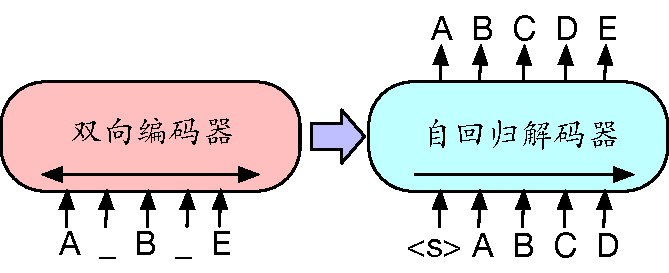
\includegraphics[scale=0.6]{\pref/bart.pdf}
    \caption{生成式语言模型BART的示意图.}
    \label{fig:autoencoder}
\end{figure}

我们已经指出,熵和编码有着密切的联系. 从这个角度出发,我们很容易理解生成模型背后的思想:我们希望通过训练的方式得到一个由神经网络所表示的编码和解码规则,他要尽可能符合真实数据的分布.

我们可以用一种非常简单的模型去理解这一过程. 假设所有的单词的集合为$\Sigma$,单词数为$k$的文本集合为$\Omega$. 我们希望训练一个生成模型$M$,给它输入$k-1$个单词,它可以给出第$k$个单词的概率分布,我们选择出现概率最大的那个词作为预测. 在训练的时候,对于一个句子$\omega$,我们只保留前$k-1$个词,得到$\omega[1:k]$,然后将它输入到生成模型$M$中,让它去预测第$k$个词. 

对于这一个具体的句子来说,理想的分布应该是一个\emph{Dirac分布}\index{Dirac分布}\footnote{Dirac分布是一个数学物理中更加常用的名字. 在概率论中,这也被称为\emph{退化分布}\index{退化分布};而在机器学习中,分布经常会表示为一个概率向量,文献中称为\emph{独热向量}\index{独热向量}. } $\delta_{\omega[k]}$,即以概率$1$取到$\omega[k]$. 假如说生成模型的输出是一个概率分布$M(\omega[1:k-1])=p$,那么,我们可以用K-L散度去衡量这两个分布的差异,因为$H(\delta_{\omega[k]})$是固定的,所以我们只考虑交叉熵$CH(\delta_{\omega[k]},p)$. 因为一次训练会给多个样本,所以我们的目标是同时最小化这些交叉熵的和. 假如训练集是$T$,我们的目标就是
\[
    \min_{M} \sum_{\omega\in T} CH(\delta_{\omega[k]},M(\omega[1:k-1])).
\]

实际上,这个例子是有普适性的,所有的监督训练的分类问题都可以用这种方式来建模. 而在 \Cref{???} 我们也会看到,此时交叉熵实际上被作为了一种\emph{损失函数}\index{损失函数}.

\section{附录:Shannon定理的证明}\label{sec:Shannon-thm-proofs}
我们在这一部分给出Shannon定理(\Cref{thm:Shannon-thm})的证明. 整体上的思路是:
\begin{enumerate}
    \item 证明如果$f$是单调函数,对正整数$m,n$成立$f(mn)=f(m)+f(n)$,那么$f(n)=C\log n$.
    \item 求出$H(1/n,\dots,1/n)$的表达式.
    \item 假设$p_i$是有理数,设$p_i=n_i/\sum_j n_j$,考虑$\sum_j n_j$个等可能试验结果,利用假设3推出$H$的表达式.
    \item 利用有理数的稠密性和$H$的连续性推出一般情形.
\end{enumerate}
最后一步是显然的,我们只需要证明前三步即可.

对第一步,我们需要证明的是,如果$f$是单调函数,对正整数$m,n$成立$f(mn)=f(m)+f(n)$,那么$f(n)=C\log n$. 首先,利用数学归纳法容易看出,对正整数$n,k$,成立
\begin{equation}
    f(n^k)=kf(n).\label{eq:Shannon-thm-proof-1}
\end{equation}

设$m,n$是任意两个大于$1$的整数,再选任意大的正整数$k$,从$m$进制数的性质可以看出,总存在正整数$l$使得
\begin{equation}
    m^l\leq n^k < m^{l+1}.\label{eq:Shannon-thm-proof-2}
\end{equation}
根据$f$的单调性,我们有
\[
    f(m^l)\leq f(n^k) < f(m^{l+1}).
\]
利用式 \eqref{eq:Shannon-thm-proof-1},我们有
\[
    lf(m)\leq kf(n) < (l+1)f(m)\iff \frac{l}{k}\leq \frac{f(n)}{f(m)} < \frac{l+1}{k}.
\]
将式 \eqref{eq:Shannon-thm-proof-2} 取对数,得到
\[
    l\log m\leq k\log n < (l+1)\log m\iff \frac{l}{k}\leq \frac{\log n}{\log m} < \frac{l+1}{k}.
\]
所以
\[
    \left|\frac{\log n}{\log m}-\frac{f(n)}{f(m)}\right|\leq\frac1k.
\]
因为$k$可以是任意大的正整数,取$k\to\infty$,我们就得到了
\[
    \frac{\log n}{\log m}=\frac{f(n)}{f(m)}.
\]
由$m,n$的任意性,取$m=2$,我们就得到了$f(n)=(f(2)/\log 2)\cdot \log n= C\log n$. 容易检验,$f(1)=0=C\log 1$,因此这一等式对所有正整数$n$都成立.

对第二步,我们需要求出$f(n)=H(1/n,\dots,1/n)$的表达式. 我们要利用第一步的结果,首先,根据假设二,$f(n)$是单调递增的函数. 然后,考虑$mn$个等可能试验,我们可以将它分成两步试验,第一步有$m$中等可能的结果,而在每一种结果之下,第二步有$n$种等可能结果. 根据假设三,
\[
f(mn)=f(m)+\frac{1}{n}\cdot nf(n)=f(m)+f(n).    
\]
所以$f(n)$符合第一步的假设. 第二步就可以直接从第一步推出.

最后,我们证明第三步. 设$p_1,\dots,p_n$都是有理数,那么,他们可以被写为
\[
    p_i=\frac{n_i}{\sum_{j=1}^n n_j}.
\]
其中$n_i$是非负整数. 我们考虑$\sum_j n_j$个等可能试验,这个试验可以被看成两步的试验,第一步有$n$种可能的结果,第$i$种结果出现的概率是$p_i$,而在第$i$种结果之下,第二步有$n_i$种等可能的结果. 根据假设三,和证明的第三步,我们有
\[
   C\log\sum_{j=1}^nn_j=H(p_1+\dots+p_n)+\sum_{i=1}^n p_i\cdot C\log n_i.
\]
因此,
\begin{align*}
    H(p_1,\dots,p_n)&=C\left(\log\sum_{j=1}^nn_j-\sum_{i=1}^n p_i\log n_i\right)\\
    &=C\left(\log\sum_{j=1}^nn_j-\sum_{i=1}^n p_i\log\left(p_i\sum_{j=1}^n n_j\right)\right)\\
    &=C\left(\log\sum_{j=1}^nn_j-\sum_{i=1}^n p_i\log p_i-\sum_{i=1}^n p_i\log\sum_{j=1}^n n_j\right)\\
    &=-C\sum_{i=1}^n p_i\log p_i.
\end{align*}
这正是我们要证明的. 于是,我们证明了Shannon定理.

\section{习题}
\begin{enumerate}[wide, labelindent=0pt]
    \item 我们在熵以及K-L散度的定义中,都规定了一些无定义的量的值,这些值并不是随便规定的,他们实际上反映了熵或者K-L散度定义中的连续性.
    \begin{enumerate}
        \item 证明:对给定的$a>0$,$\lim_{x\to 0+}x\log (x/a)=0$,因此我们规定了$0\log 0=0$以及$0\log(0/a)=0$.
        \item 证明:对给定的$a>0$,$\lim_{x\to 0+}x\log (a/x)=+\infty$,因此我们规定了$0\log(a/0)=+\infty$.
    \end{enumerate}
    
    \item 考虑关于$n$的正实数序列$a_1(n),\dots,a_k(n)$以及$b_1(n),\dots,b_k(n)$,假设对所有$i$,都成立$\lim_{n\to\infty} a_i(n)/b_i(n)=1$,证明:
    \[\lim_{n\to\infty}\frac{a_1(n)+\dots+a_k(n)}{b_1(n)+\dots+b_k(n)}=1.\]
    由此证明式 \eqref{eq:logP}.
    
    \item 证明\Cref{prop:entropy-2prob}.
    
    \item 用Lagrange乘子法重新证明\Cref{prop:entropy-maximum}.
    \begin{hint}
        如果你不知道Lagrange乘子法,可以参考 \Cref{???}.
    \end{hint}

    \item 证明\Cref{prop:conditional-mutual-information}.
    
    \item \cite{tingAmountInformation1962a} 仿照集合论的思路,我们可以定义三个随机变量的互信息为:
    \[I(X;Y;Z)=I(X;Y)-I(X;Y|Z).\]
    \begin{enumerate}
        \item 证明对称性:$I(X;Y;Z)=I(Y;X;Z) = I(X;Z;Y)$.
        \item 举一个例子说明,可能会有$I(X;Y;Z)<0$,所以这样定义的互信息并不一定真的代表“信息量”.
    \end{enumerate}

    \item 举一个例子说明,即便$D(p_1\Vert p_2)$很接近$0$,$D(p_2\Vert p_1)$也可能会很大.
    
    \item (\emph{单变量数据处理不等式})对任意离散随机变量$X$和函数$f$,证明:$H(X)\geq H(f(X))$.

    \item 考虑二分类的学习问题,此时对单个样本我们观察到的结果要么是$0$或$1$,假设在真实世界中样本总体服从参数为$\theta$的Bernoulli分布\index{Bernoulli分布},即$\Pr(X=1)=1-\Pr(X=0)=\theta$. 假设我们的数据集是$(x_1,y_1),\dots,(x_N,y_N)$,他们是从总体中独立采样得到的. 
    \begin{enumerate}
        \item 将问题考虑成一个数理统计问题,估计$\theta$. 写出似然函数\index{似然函数}$L(\theta;y_1,\dots,y_N)$.
        \item 再将问题考虑为一个信息论问题,写出每个样本的真实分布与估计分布之间的交叉熵之和$CH(\theta;y_1,\dots,y_N)$.
        \item 证明:$\max_{\theta} L(\theta;y_1,\dots,y_N)=\min_{\theta} CH(\theta;y_1,\dots,y_N)$,也就是说,\emph{最大似然估计等价于最小化交叉熵}.
    \end{enumerate}

    \item 请查找文献回答以下问题:
    \begin{enumerate}
        \item Fisher信息量是什么?它与K-L散度有什么样的关系?
        \item 列举其他概率分布之间散度的概念,他们是否是度量?
        \item 列举概率分布之间的度量,他们之间是否有关联?
    \end{enumerate}
    
\end{enumerate}
\section{章末注记}
信息一词的英文是“information”,从动词“inform”来,意思是告知、通知. 早在15世纪中叶,“information”一词的出现了义项“在通信中针对特定主题的知识”.\cite{InformationEtymologyOrigin} 这说明在那个时候人类就已经意识到,通信会产生新的东西,被称为知识或信息. 然而,人类对信息的严谨探索起步晚得多. 关于信息的物理学讨论源自统计力学,Boltzmann提出了著名的熵,证明了H定理,以此给出了热力学第二定律的微观解释. 关于Boltzmann的工作,参见 \cite{uffinkBoltzmannWorkStatistical2022}. 

一般认为,现代信息论的起源是Shannon的论文 \cite{shannonMathematicalTheoryCommunication1948},他在论文中提出了信息的数学定义,以及信息的基本性质. 但是,Shannon的工作并不是孤立的,他的工作是在统计力学的基础上发展起来的. 事实上,Shannon在论文中也提到了Boltzmann的熵. 这篇工作也被视为通信理论以及编码理论的奠基性工作.  Shannon在这篇论文中还给出了渐近意义下达到理论下界的最优编码,并且独立地被Fano \cite{robertm.fanoTransmissionInformation1949} 以一种不同的形式发现,因此后世称为Shannon-Fano编码. 但是Shannon-Fano编码并不是精确地达到下界,实际上,最优编码是Huffman \cite{huffmanMethodConstructionMinimumRedundancy1952} 给出的. Shannon在这篇论文中还讨论了渐近等分性,后来MciMillan的工作 \cite{mcmillanBasicTheoremsInformation1953} 和 Breiman的工作 \cite{breimanIndividualErgodicTheorem1957} 拓展了这一结果,因此后世称为Shannon-McMillan-Breiman定理. 

关于信息论与集合论的关系工作,可以参见Hu Kuo Ting的工作 \cite{tingAmountInformation1962a}. 他的工作还给出了多个随机变量互信息的定义,在这一章习题中有涉及.

相对熵的概念依然是从Shannon的奠基性论文 \cite{shannonMathematicalTheoryCommunication1948} 中提出的,但他只局限于通信的问题. 更加一般的讨论是由Kullback和Leibler在 \cite{kullbackInformationSufficiency1951} 给出,他们的是一种数理统计的思路,但是他们也具体地讨论了这一概念与信息的关系. 他们的论文中也讨论了交叉熵这一概念. 

机器学习中编码器和解码器的思路,最早是由Rumelhart,Hinton和Williams在 \cite{rumelhartLearningInternalRepresentations1986} 中提出,他们将编码器和解码器的整体称作\emph{自编码器}. 这篇工作几乎可以被视为深度学习的开山之作,它还提出了训练神经网络最常用的反向传播算法.

关于信息论的经典教科书,可以参见 \cite{coverElementsInformationTheory2012} ,此外,概率论的教材中也有很多很好的讨论,比如 \cite{jaynesProbabilityTheoryLogic2002},\cite{shiryaevProbability1996} 以及\cite{LiXianPingGaiLuLunJiChu2010}.

关于Kolmogorov复杂度的讨论,可以参见专著 \cite{???},这本书对于随机、信息、编码、复杂度,乃至归纳推理等概念都有非常独到的见解,值得一读. 

\endgroup
\chapter{信息论基础}\label{chap:information-theory}
\begingroup
\newcommand{\pref}{Chapters/information-theory/figures}

信息是什么?不同于真实的物理世界,信息仿佛看不见,摸不着. 然而,任何人都可以体会到信息的存在,信息是我们认识世界的基础. 信息的存在正如同物理世界中的能量、动量一般,抽象而具有一般性. 信息论已经在计算机、AI、认知理论等诸多领域中得到了广泛的应用. 本章探讨信息论的基础,并给出他们在AI中的一些应用. 

在\Cref{sec:entropy},我们讨论熵的概念与性质. 在\Cref{sec:kl-divergence},我们讨论Kullback-Leibler散度的概念与性质. 在\Cref{sec:Shannon-thm-proofs},我们给出Shannon定理证明. 

\section{熵}\label{sec:entropy}


\subsection{概念的导出}

我们常说“恐惧来源于未知”,信息似乎代表着某种确定的东西,某种知识,因而和不确定性有相反的关系. 更精确地说,\emph{消除不确定性的东西被称为信息.} 当然,这句话本身似乎是一种循环论证,它并没有真正回答信息或者不确定性到底是什么. 所以我们进一步的问题是,给定一个“对象”,如何定量衡量它不确定性(或信息量)?

然而,单个对象的信息是一个非常难以划定的概念. 同样的内容,对于不同的人来说,信息量是完全不同的. 比如说,已经学过信息论的读者再看这一部分内容,他获得的信息一定比没有学过的读者要少得多. 因而实际上,一种更加容易的办法是我们将世界视为不确定的,因而有多种可能的对象,然后考虑这一堆对象的信息量. 比如说,这本书的读者的背景是不确定的,可能学过信息论,也可能没学过,但是我们可以综合考虑不同读者的背景,然后给出一个信息的概率分析. 

我们可以用数学来表述上面的考虑,假如我们进行一次试验,一共有$n$种可能的结果,第$i$种发生的概率为$p_i$. 我们预测试验的结果,如果越能正确地预测,那么就说明我们对这个试验中包含的信息知道的越多. 假如$p_1=1$,那么我们完全确定试验一定会产生结果$1$. 如果$p_i=1/n$,那么我们完全无法预计试验的结果. 我们对试验结果的预期与试验结果的概率分布有密切联系. 因此概率分布给我们带来了\textbf{信息}\index{信息},使得我们能够产生不同的判断. 另一方面,概率分布带来了\textbf{不确定性}\index{不确定性},使我们不能总是确信预言会成真. 

我们遵循“信息论之父”Shannon的思路,为信息提供一个严格的数学模型:熵. 假设随机变量$X$表示了所有可能的结果(编号为$1$到$n$),$\Pr(X=i)=p_i$,$p=(p_1,\dots,p_n)$,有时候也把$p_i$写作$p(i)$. 我们把不确定性度量记为$H(p)$. Shannon假设$H$满足以下三个性质:
\begin{enumerate}
    \item $H$是一个连续函数.
    \item 事件结局可能数变多则不确定性增大:$p_i=1/n$时,$H(p)$随$n$单调递增,$n$是正整数.
    \item 如果一个试验被分成了两个相继的试验,那么原来的$H$应该等于分开之后的$H$的加权和.
\end{enumerate}

\begin{remark}
    第三个假设可以用下图来理解. 
\begin{center}
\documentclass{standalone}
% font set
\usepackage{ctex}
\usepackage{fontspec}
\usepackage[T1]{fontenc}
\usepackage[sc]{mathpazo}
\usepackage{anyfontsize}
\setmainfont{Source Serif 4}
\setsansfont{Source Sans 3}
\setmonofont{Menlo}
\setCJKmainfont[BoldFont=黑体-简 中等,ItalicFont=楷体-简 常规体]{宋体-简 常规体}

% colors
\usepackage[dvipsnames]{xcolor}
\definecolor{pku-red}{RGB}{139,0,18}
\usepackage{colortbl}
\newcommand{\light}[1]{\textcolor{Orchid}{#1}}
\newcommand{\contrastlight}[1]{\textcolor{TealBlue}{#1}}

% plots
\usepackage{tikz}
\usepackage{tikz-cd}
\usetikzlibrary{arrows}
\usetikzlibrary{arrows.meta,positioning,calc,3d}
\usepackage{pgfplots}
\pgfplotsset{compat=newest}
\tikzset{
    punkt/.style={
        rectangle,
        rounded corners,
        draw=black, very thick,
        minimum height=2em,
        inner sep=6pt,
        text centered,
        fill=gray!30
    }
}

% math package
\let\Bbbk\relax
\usepackage{amsmath}
\usepackage{mathrsfs}
\usepackage{amssymb}
\usepackage{amsfonts}
\usepackage{stmaryrd}
\usepackage{latexsym}
\usepackage{extarrows}
\SetSymbolFont{stmry}{bold}{U}{stmry}{m}{n}
\begin{document}
\begin{tikzpicture} [
  level distance=2cm,
  grow'=right,
  level 1/.style= {sibling distance=0.8cm},
  solid node/.style= {circle,draw,inner sep=1.5,fill=black},
  edge from parent/.style={very thick,draw}
]
\node (0) [solid node] {}
  child {node (A1) [solid node,label=right: {$1$}] {} edge from parent node [above] {\scriptsize $1/2$}}
  child {node (A2) [solid node,label=right: {$2$}] {} edge from parent node [above right] {\scriptsize $1/3$}}
  child {node (A3) [solid node,label=right: {$3$}] {} edge from parent node [below] {\scriptsize $1/6$}};
\end{tikzpicture}
\qquad
\begin{tikzpicture} [
  level distance=1cm,
  grow'=right,
  level 1/.style= {sibling distance=1cm},
  level 2/.style= {sibling distance=0.8cm},
  solid node/.style= {circle,draw,inner sep=1.5,fill=black},
  edge from parent/.style={very thick,draw}
]
\node (0) [solid node] {}
  child {node (A1) [solid node,label=right: {}] {} 
  child {node (B1) [solid node,label=right: {$1$}] {} edge from parent node [above] {\scriptsize $1$}}
  edge from parent node [above]{\scriptsize $1/2$}
    }
  child {node (A2) [solid node,label=right: {}] {} 
  child {node (B2) [solid node,label=right: {$2$}] {} edge from parent node [above] {\scriptsize $2/3$}}
  child {node (B3) [solid node,label=right: {$3$}] {} edge from parent node [below] {\scriptsize $1/3$}}
  edge from parent node [below] {\scriptsize $1/2$}
  };
  
\end{tikzpicture}
\end{document}
\end{center}

    假设我们有一个试验,有三种可能的结果,$1,2,3$,概率分别为$1/2,1/3,1/6$. 该试验的不确定性是$H(1/2,1/3,1/6)$. 我们把试验分成两步相继的试验,第一步试验有两种可能的结果,概率分别都是$1/2$. 当第一步试验出现上面的结果时,第二步试验以概率$1$产生结果$1$;当第二步试验出现下面的结果时,第二步试验以概率$2/3$产生结果$2$,以概率$1/3$产生结果$3$. 我们可以看到,分成两步之后,第一步试验的不确定性是$H(1/2,1/2)$,第二步试验的不确定性有一半概率是$H(1)$(上面的分支),有一半概率是$H(2/3,1/3)$(下面的分支),因而加权的不确定性是$1/2\cdot 0+1/2\cdot H(2/3,1/3)$. 因此第三个假设可以具体表述为
\[
H\left(\frac{1}{2},\frac{1}{3},\frac{1}{6}\right)=H\left(\frac{1}{2},\frac{1}{2}\right)+\left[\frac{1}{2}\cdot H(1)+\frac{1}{2}\cdot H\left(\frac{2}{3},\frac{1}{3}\right)\right].
\]
\end{remark}

这里,我们可以看出Shannon的哲学思想:不确定性只来自于概率分布而不是具体对象. 他的考虑具有浓厚的工程意味,正如他自己针对通信的数学理论所说:“消息是具有含义的……然而,通信的语义层面并不是工程问题所关心的. “正是因为抽象掉了具体考虑的对象,信息论的应用才变得如此广泛. 

基于上面三个假设,Shannon证明了如下定理,这一定理直接给出了熵的概念.

\begin{theorem}[Shannon定理]\label{thm:Shannon-thm}
    $H$满足三个假设当且仅当
    \[H(p)=-C\sum_{i}p_i\log p_i,\]
    其中$C$是正常数,$0\log 0=0$.
\end{theorem}
这一定理的证明较长并且和后面的讨论关联较小,所以我们在\Cref{sec:Shannon-thm-proofs} 中给出证明.

根据对数的的换底公式,可以将$C\log p_i$写为$\log_bp_i$,这里$C=1/\log b$. 于是,Shannon定理直接给出了熵的如下定义:
\begin{definition}[熵]
    分布列$p=(p_1,\dots,p_n)$的\textbf{熵}\index{熵}定义为
    \[H(p)=-\sum_{i=1}^np_i\log_b p_i.\]
    其中$b=\e$(自然对数底数),$0\log 0=0$. 当$b=2$时,我们记熵为$H_2(p)$.
\end{definition}

通常来说,使用$\e$作为底数会使得数学推导简洁,而用$2$为底数则常常是讨论信息量时的习惯. 在后面通信理论中,我们将讨论熵在通信中的含义,以$2$为底的时候熵的实际意义会更清楚些. 如果没有特别强调,我们在讨论时总是假设$b=\e$.

熵的定义还可以用数学期望的形式写出. 假设$X$的分布列是$p$,$p(i)=\Pr(X=i)$,那么我们也可以把熵写成期望的形式:
\[H(p)=-\E[\log p(X)].\]
每一个(离散)随机变量$X$会确定一个分布列$p_X$,因此我们也可以定义随机变量的熵:
\begin{definition}[随机变量的熵]
    随机变量$X$的\textbf{熵}\index{熵!随机变量的~}定义为
    \[H(X)=-\E[\log p_X(X)].\]
    其中$p_X$是$X$的分布列,$0\log 0=0$.
\end{definition}

尽管从信息论的角度我们可以唯一确定熵的定义,但是熵的概念在物理学上早就已经存在. 下面我们给出统计力学中熵的推导过程. 在经典力学中,物理系统的状态由粒子的位置和动量(速度)完全确定,将粒子位置和动量可能的值集合称为\emph{相空间},于是物理系统的演化就是相空间中的粒子状态的变化. 将相空间等分成$m$个单元,编号$1$到$m$. 假设相空间中有$N$个可区分的粒子,相互独立,没有相互作用,每个粒子等可能出现在每一个单元中. 如果单元$i$中有$N_i$个粒子,那么按照粒子在单元中的分布来看,系统处于某个特定状态的概率为
    \[P=\frac{N!}{N_1!\dots N_m!}\left(\frac1m\right)^N.\]
这是一个多项分布. 两边取对数,得
    \[\log P=\log(N!)-\sum_i\log(N_i!)-N\log m.\]
考虑充分大的$N_i$,由Stirling公式,有
\begin{align*}
    \log(N_i!)\sim\log\left(\sqrt{2\pi N_i}\left(\frac{N_i}{\e}\right)^{N_i}\right)\sim N_i\log N_i.    
\end{align*}
因此,
\begin{equation}
    \log P\sim N\log N-\sum_i N_i\log N_i- N\log m\sim N\log N-\sum_i N_i\log N_i.\label{eq:logP}
\end{equation}
假设$N_i$充分大的时候,$N_i/N$呈现固定的比例$p_i$,那么
    \begin{align*}
        N\log N-\sum_i N_i\log N_i&\sim N\log N-\sum_i Np_i\log(Np_i)\\
        &=-N\sum_i p_i\log p_i.
    \end{align*}
 $\log P\sim -N\sum_i p_i\log p_i$. 于是我们证明了:
    \[\frac1N\log P\to H(p_1,\dots,p_m),\quad N\to\infty.\]
因此,熵刻画了充分多粒子的物理系统某种特定状态出现概率!熵越大的系统越有可能达到. 更进一步,在统计力学中有Boltzmann $H$-定理:孤立的粒子系统会向着熵($H$)增加的方向演化,并最终达到熵最大的状态. $H$-定理是热力学第二定律的微观解释,熵越大的系统出现概率越大、越混乱、越接近均衡.

\subsection{概念与性质}
现在,我们将进一步探讨熵的若干拓展定义,并讨论他们的性质. 

首先,我们考虑最简单的情形,即分布列为$(p_1,p_2)$,此时,我们不妨设$p_1=p$,$p_2=1-p$,那么熵就是
    \[H(p_1,p_2)=H(p,1-p)=-p\log p-(1-p)\log(1-p).\]
$H$是关于$p$的函数,作图如\Cref{fig:entropy-figure} 所示.
\begin{figure}[ht]
        \centering
        \documentclass{standalone}
% font set
\usepackage{ctex}
\usepackage{fontspec}
\usepackage[T1]{fontenc}
\usepackage[sc]{mathpazo}
\usepackage{anyfontsize}
\setmainfont{Source Serif 4}
\setsansfont{Source Sans 3}
\setmonofont{Menlo}
\setCJKmainfont[BoldFont=黑体-简 中等,ItalicFont=楷体-简 常规体]{宋体-简 常规体}

% colors
\usepackage[dvipsnames]{xcolor}
\definecolor{pku-red}{RGB}{139,0,18}
\usepackage{colortbl}
\newcommand{\light}[1]{\textcolor{Orchid}{#1}}
\newcommand{\contrastlight}[1]{\textcolor{TealBlue}{#1}}

% plots
\usepackage{tikz}
\usepackage{tikz-cd}
\usetikzlibrary{arrows}
\usetikzlibrary{arrows.meta,positioning,calc,3d}
\usepackage{pgfplots}
\pgfplotsset{compat=newest}
\tikzset{
    punkt/.style={
        rectangle,
        rounded corners,
        draw=black, very thick,
        minimum height=2em,
        inner sep=6pt,
        text centered,
        fill=gray!30
    }
}

% math package
\let\Bbbk\relax
\usepackage{amsmath}
\usepackage{mathrsfs}
\usepackage{amssymb}
\usepackage{amsfonts}
\usepackage{stmaryrd}
\usepackage{latexsym}
\usepackage{extarrows}
\SetSymbolFont{stmry}{bold}{U}{stmry}{m}{n}

\begin{document}
\begin{tikzpicture}
    \pgfplotsset{
    width=8cm,
    every axis/.append style={very thick},
    }
    \begin{axis}[
        ymin=0, ymax=0.8,
        xmin=0, xmax=1.05,
        axis x line=left,
        axis y line=left,
        legend style={draw=none},
        xtick={0,0.25,0.5,0.75,1},
        ytick={0,0.2,0.4,0.6},
        legend pos=south east,
        every axis x label/.style={
            at={(ticklabel* cs:1.02)},
            anchor=north west,
        },
        every axis y label/.style={
            at={(ticklabel* cs:0.95)},
            anchor=west,
        },
        label style={font=\normalfont},
        xlabel={$x$},ylabel={$H(p,1-p)$}
    ]
    \addplot[domain =0:1, smooth] {-x*ln(x)-(1-x)*ln(1-x)};
    \end{axis}
\end{tikzpicture}
\end{document}
        \caption{熵$H(p)$的图像.}
        \label{fig:entropy-figure}
\end{figure}

利用导数的方法,很容易证明:
\begin{proposition}\label{prop:entropy-2prob}
    $H(p)$在$p\in (0,1/2)$严格单调递增,在$p\in (1/2,1)$严格单调递减. 它的最小值是$0$,在$p\in\{0,1\}$取得;它的最大值是$\log 2$,在$p=1/2$取得.    
\end{proposition}

 这与我们对于“不确定性”的直觉是相一致的:当$p$接近$0$或$1$时,我们对于$X$的取值几乎是确定的,因此熵接近$0$;当$p$接近$1/2$时,我们对于$X$的取值几乎是完全不确定的,因此熵接近最大值$\log 2$. 实际上,这样的性质对于一般的分布也是成立的.

考虑一般分布的熵$H(p)=H(p_1,\dots,p_n)$. 我们有如下性质:
\begin{proposition}\label{prop:entropy-nonnegative}
    $H(p)\geq 0$,等号成立当且仅当某个$p_i=1$.
\end{proposition}
\begin{proof}
这是一个典型的证明,主要的技巧是使用熵的期望形式. 考虑随机变量$X$,其分布列为$p$. 回忆Jensen不等式:如果$f$是一个严格凸函数,那么
\[\E[f(X)]\geq f(\E[X]).\]
等号成立当且仅当$X$是常数.

因为$-\log(\cdot)$是严格凸函数,所以根据Jensen不等式
\[H(X)=\E[-\log p(X)]\geq-\log\E[p(X)]\geq -\log 1=0.\]
等号成立当且仅当$X$是常数,即对某个$i$,$p(i)=1$.
\end{proof}

\begin{proposition}\label{prop:entropy-adjust}
    $p_i$朝着相等方向改变的时候$H$增加. 也就是说,假设$p_i<p_j$,再假设$p_i'>p_i,p_j'<p_j$且$p_i+p_j=p_i'+p+j'$. 用$p_i'$和$p_j'$代替原来的$p_i$和$p_j$,那么$H$变大. 
\end{proposition}
\begin{proof}
    为简化符号,考虑$i=1$和$j=2$. 利用假设三,第一步试验中,将试验的结果$1$和结果$2$合并,第二步试验再按照$p_1/(p_1+p_2)$和$p_2/(p_1+p_2)$的概率产生结果$1$和结果$2$. 于是,
    \begin{align*}
        &H(p_1,p_2,\dots)\\
        =&H(p_1+p_2,p_3,\dots)+(p_1+p_2)H\left(\frac{p_1}{p_1+p_2},\frac{p_2}{p_1+p_2}\right)\quad(\text{假设三})\\
       \leq &H(p_1+p_2,p_3,\dots)+(p_1+p_2)<H\left(\frac{p_1'}{p_1'+p_2'},\frac{p_2'}{p_1'+p_2'}\right)\quad(\text{\Cref{prop:entropy-2prob}})\\
       =&H(p_1',p_2',p_3,\dots).\quad(\text{假设三})
    \end{align*}
\end{proof}

\begin{proposition}\label{prop:entropy-maximum}
    当$p_1=\dots=p_n=1/n$时$H$取得最大值$\log n$.
\end{proposition}
\begin{proof}
   若存在$p_i\ne p_j$,因为$\sum_i p_i/n=1/n$,根据鸽巢原理,则必有$i,j$满足$p_i<1/n<p_j$. 根据\Cref{prop:entropy-adjust},我们可以将$p_i$和$p_j$替换为$1/n$和$p_i+p_j-1/n$,而$H$增大. 只要还有两个$p_i$不相等,这一过程就可以重复,每一次都会增大$H$,直到所有$p_i$都等于$1/n$.
\end{proof}

至此,\Cref{prop:entropy-nonnegative} 和\Cref{prop:entropy-maximum} 证明了一般情形的\Cref{prop:entropy-2prob}. 在等可能的时候不确定性最大,熵最大;在确定事件的时候不确定性最小,熵最小. 所以熵是符合直观的定义. 

接下来,我们讨论熵的拓展形式.

在一次试验中,我们可以观察多个变量,比如说$X$和$Y$. 我们也可以说,我们观察到了一个结果$(X,Y)$,服从分布$p(i,j)$. 因此有对应的熵,这就是\textbf{联合分布的熵}\index{熵!联合分布的~}:
    \[H(X,Y)=-\E[\log p(X,Y)].\]
对应地,我们也可以写成和的形式:
    \[H(p)=-\sum_{i,j}p(i,j)\log p(i,j).\]
自然,联合分布也可以引出\textbf{边缘分布的熵}\index{熵!边缘分布的~}:
\[H(X)=-\E[\log p_X(X)]=-\sum_i \sum_j p(i,j)\log \sum_j p(i,j).\]
\[H(Y)=-\E[\log p_Y(Y)]=-\sum_j \sum_i p(i,j)\log \sum_i p(i,j).\]

有了两个随机变量,我们就可以讨论“条件”的概念. 具体来说,我们可以把试验分为两步,第一步观测$X$,第二步观测$Y$,那么,第二步所产生的熵就是已经知道第一步结果之后的熵,即:
\[H(Y| X=x)=-\E[\log p_{Y| X=x}(Y)| X=x]=-\sum_{j}p_{Y|X=x}(j)\log p_{Y|X=x}(j),\]
其中$p_{Y|X=x}(j)=p(x,j)/p_X(x)$. 当我们知道了$X=x$之后,对$Y$的观测就消除了部分的不确定性,因此根据我们对于不确定性和信息关系的讨论,从$X=x$中获得的关于$Y$的信息是
\[I(X=x:Y)=H(Y)-H(Y|X=x).\]
考虑一个特殊情况,$Y=X$,那么刚刚的讨论就变成了自己从自己身上获得的信息,或者说知道$X=x$带来的信息量. 首先有
\[p_{X|X=x}(i)=\begin{cases}
    1,&i=x\\
    0,&i\ne x.
\end{cases}\]
因此,
\[H(X| X=x)=-\sum_{j}p_{X|X=x}(j)\log p_{X|X=x}(j)=-1\log 1=0.\]
于是,
\[I(X=x:X)=H(X)-H(X|X=x)=H(X).\]
这正是定量版本的“消除不确定性的东西被称之为信息”!此外,我们之前说过,熵刻画的是一族可能对象的信息,这一点也反映在了这一公式中:只要知道了$X$的值,无论它具体是多少,我们得到的信息量是一样的!

再回到一般情况,还是同样的两步试验,我们定义给定$X$时$Y$的\textbf{条件熵}\index{熵!条件~}为
\begin{align*}
    H(Y| X)=&\E[H(Y|X=x)]\\
    =&-\E[\log p_{Y| X}(Y)]\\
    =&-\sum_x p_{X}(x)\sum_{j}p_{Y|X=x}(j)\log p_{Y|X=x}(j)\\
    =&-\sum_{x,j}p(x,j)\log p_{Y|X=x}(j).
\end{align*}
换言之,我们现在进一步假定$X$也是不知道的,于是$H(Y|X)$就是平均上来说第二步中$Y$的不确定性. 条件熵和熵有着类似的性质:
\begin{proposition}\label{prop:conditional-entropy-nonnegative}
    $H(Y|X)\geq 0$,等号成立当且仅当$Y$是退化的,即$Y$概率$1$只取一个值.
\end{proposition}
\begin{proof}
    仿照\Cref{prop:entropy-nonnegative} 的证明即可.
\end{proof}
类似地,我们可以考虑平均上$Y$中包含的关于$X$的信息量:
\[\E[I(X=x:Y)]=H(Y)-H(Y|X).\]
与之相对应地,平均上$X$中包含的关于$Y$的信息量为
\[\E[I(Y=y:X)]=H(X)-H(X|Y).\]
一个自然的问题是,二者相互包含的信息量是什么关系?根据概率的链式法则,$p(x,y)=p_{X|Y}(x|y)p_Y(y)$,带入$H(X,Y)$的定义得熵的链式法则:

\begin{proposition}\label{prop:entropy-chain-rule}
    对任意离散随机变量$X,Y$,$H(X,Y)=H(Y)+H(X|Y)$.    
\end{proposition}

利用链式法则,我们注意到,$H(X)-H(X|Y)=H(X)-(H(X,Y)-H(Y))=H(X)+H(Y)-H(X,Y)=H(Y)-H(Y|X)$. 所以,$X$中包含的$Y$的信息和$Y$中包含的$X$的信息是一样多的!此外,直观上我们还应该觉得,信息量不能是负的,实际上的确如此:
\begin{proposition}\label{prop:information-doesnt-hurt}
    $H(X)-H(X|Y)\geq 0$,等号成立当且仅当$X$和$Y$相互独立.
\end{proposition}

我们将在\Cref{sec:kl-divergence}看到,\Cref{prop:information-doesnt-hurt} 就是K-L散度信息不等式的一个特例,所以我们就不在这里给出证明了. \Cref{prop:information-doesnt-hurt} 表明知道任何信息都不会增加不确定性,这个原理被称为“Information doesn't hurt.” 根据以上讨论,我们可以自然地定义$X$和$Y$的\textbf{互信息}\index{互信息}为$I(X;Y)=I(Y;X)=\E[I(X=x:Y)]=\E[I(Y=y:X)]$.

类似联合分布的熵,条件熵和互信息的概念也可以推广到多元情形. 对于三个随机变量$X,Y,Z$,我们可以定义条件熵为
\[H(X,Y|Z)=H(X,Y,Z)-H(Z).\]
类似地,我们可以定义互信息为
\[I(X,Y;Z)=H(X,Y)-H(X,Y;Z).\]
他们的含义以及性质和二元情形类似.

同样,我们可以定义\textbf{条件互信息}\index{条件互信息}为$I(X;Y|Z)=H(X|Z)-H(X|Y,Z)$,表明$Z$已知时候$Y$给$X$带来的平均信息增益. 类似互信息,我们如下性质:
\begin{proposition}\label{prop:conditional-mutual-information}
    条件互信息满足以下性质:
    \begin{enumerate}
        \item 非负性:$I(X;Y|Z)\geq 0$,等号成立当且仅当$X$和$Y$在给定$Z$的条件下相互独立.
        \item 对称性:$I(X;Y|Z)=I(Y;X|Z)$.
        \item 链式法则:$I(X,Y;Z)=I(X;Z|Y)+I(Y;Z)$.
        \item 条件信息量:$I(X:X|Y)=H(X|Y)-H(X|X,Y)=H(X|Y)$.
    \end{enumerate}
\end{proposition}
最后一条性质说的其实是,在平均的意义下,给定$Y$的时候,知道$X$所能够得到的额外信息量就是$H(X|Y)$. 这一命题的证明和前面都非常相似,我们留做习题.

最后,我们将各种熵以及信息量的关系总结为\Cref{fig:entropy-relation}. 在集合论中,这样的图被称为Venn图,所以我们可以用集合论来理解信息与熵. 对应关系可以总结为\Cref{tab:entropy-relation}.
\begin{table}[ht]
    \centering
        \begin{tabular}{c|c}
        \toprule
        信息论&集合论\\
        \midrule
        $H(X)$&$A$\\
        $H(Y)$&$B$\\
        $H(X|Y)$&$A\setminus B$\\
        $H(X,Y)$&$A\cup B$\\
        $I(X;Y)$&$A\cap B$\\
        \bottomrule
        \end{tabular}
    \caption{信息论和集合论的对应关系.}
    \label{tab:entropy-relation}
\end{table}
\begin{figure}[ht]
    \centering
    \documentclass{standalone}
% font set
\usepackage{ctex}
\usepackage{fontspec}
\usepackage[T1]{fontenc}
\usepackage[sc]{mathpazo}
\usepackage{anyfontsize}
\setmainfont{Source Serif 4}
\setsansfont{Source Sans 3}
\setmonofont{Menlo}
\setCJKmainfont[BoldFont=黑体-简 中等,ItalicFont=楷体-简 常规体]{宋体-简 常规体}

% colors
\usepackage[dvipsnames]{xcolor}
\definecolor{pku-red}{RGB}{139,0,18}
\usepackage{colortbl}
\newcommand{\light}[1]{\textcolor{Orchid}{#1}}
\newcommand{\contrastlight}[1]{\textcolor{TealBlue}{#1}}

% plots
\usepackage{tikz}
\usepackage{tikz-cd}
\usetikzlibrary{arrows}
\usetikzlibrary{arrows.meta,positioning,calc,3d}
\usepackage{pgfplots}
\pgfplotsset{compat=newest}
\tikzset{
    punkt/.style={
        rectangle,
        rounded corners,
        draw=black, very thick,
        minimum height=2em,
        inner sep=6pt,
        text centered,
        fill=gray!30
    }
}

% math package
\let\Bbbk\relax
\usepackage{amsmath}
\usepackage{mathrsfs}
\usepackage{amssymb}
\usepackage{amsfonts}
\usepackage{stmaryrd}
\usepackage{latexsym}
\usepackage{extarrows}
\SetSymbolFont{stmry}{bold}{U}{stmry}{m}{n}

\begin{document}
\begin{tikzpicture}[thick, scale=1.5]
    \draw [fill opacity=0.5,fill=green] (1,1) ellipse (1.25 and 1);
    \draw [fill opacity=0.5,fill=red] (2.5,1) ellipse (1.25 and 1);
    
    \draw [fill opacity=0.5,fill=green] (-1,2.5) ellipse (1.25*0.2 and 1*0.2);
    \node at (-0.3,2.5) {$H(X)$};

    \draw [fill opacity=0.5,fill=red] (-1+2,2.5) ellipse (1.25*0.2 and 1*0.2);
    \node at (-0.3+2,2.5) {$H(Y)$};

    \draw [fill opacity=0.5,fill=green] (-1+4,2.5) ellipse (1.25*0.2 and 1*0.2);
    \draw [fill opacity=0.5,fill=red] (-1+4+1.5*0.2,2.5) ellipse (1.25*0.2 and 1*0.2);
    \node at (0.2+4,2.5) {$H(X,Y)$};

    \node at (1.75,1) {$I(X;Y)$};
    \node at (0.5,1) {$H(X|Y)$};
    \node at (3,1) {$H(Y|X)$};
\end{tikzpicture}
\end{document}
    \caption{熵和信息量的关系.}
    \label{fig:entropy-relation}
\end{figure}

\subsection{熵与通信理论}\label{subsec:entropy-and-communication}
最早的时候,Shannon建立信息论,就是为了给通信理论一个数学基础. 从通信的角度出发,我们可以更本质地理解信息和熵. 

通信就是一个发射端和一个接收端,中间有信道传递消息. 将所有可能要传递的消息集合记为$\Omega$(一个有限集),我们现在考虑$\Omega$所蕴含的信息量是多少. 注意到,根据Shannon的思想,$\Omega$里面具体是什么并不重要,重要的是有多少个. 我们可以用自然数$1,2,\dots$表示集合$\Omega$里的元素. 那么,使用二进制编码,我们至少需要$\log_2 |\Omega|$个比特来表示$\Omega$里的元素. 于是,假如说随机变量$X$表示收到的消息,那么$X$的熵\index{熵}就定义为$H(X)=\log_2 |\Omega|$,它衡量了接收端收到的消息的不确定性. 当我们选定了具体的消息$m\in \Omega$,$X$的不确定性被消除了,于是$X=a$的过程产生了(或者说传递了)$\log_2 |\Omega|$比特的信息. 比如说,我们发送一个长为 $n$ 的二进制序列,消息的集合大小就是$2^n$,发送任何一条具体的消息,我们就传递了 $n$ 比特的信息.

有时候,我们会把消息看成一个序列. 具体来说,我们可以发送独立的$k$条消息,其中第$i$条$X_i$来自消息集合$\Omega_i$,$|\Omega_i|=n_i$,那么$(X_1,\dots,X_k)$的熵就是
\[H(X_1,\dots,X_k)=\log_2 n_1+\dots+\log_2 n_k,\]
它衡量了$k$条消息的不确定性. 在更常见的情况下,每次发送的其实不是一条消息,而是一个字母,所有的字母组成了一个字母表,我们用$\Sigma=\{x_1,\dots,x_s\}$来表示. 于是,$X_i$就是消息的第$i$个字母,于是,一条消息可以写作$X_1\dots X_k$,其中每一个$X_i$都来自$\Sigma$.

我们现在考虑更加简单的情形,即每一个字母$X_i$其实是同一个随机变量$X$的独立采样. 如果我们具体知道某一个$x_i$出现的次数,那么我们其实可以有更高效的传递信息的方式. 譬如说,在极端情况下,如果只有$x_1$和$x_2$会出现,那么我们其实只需要$\log_2 2=1$比特就足够传递所有消息了. 在一般情况下,考虑$\Omega$中只包含长为$k$的消息,并且$x_i$在消息中出现$k_i$次,那么所有可能的消息数量为
\[N(k)=\frac{k!}{k_1!\cdot\dots\cdot k_s!}.\]
假定我们需要$h(\omega)$比特来具体确定发的消息是$\omega$. 首先,无序集合本身需要$\log_2 |\Omega|$比特来编码,其次,我们还需要确定$(k_1,\dots,k_s)$,确定它的一种方式是按照顺序给出每一个$k_i$. 每个$k_i$最多需要$\log_2 k$比特来表示,所以按顺序表示所有的$k_i$至多需要$s\log_2 k$比特. 于是,我们需要的比特数为
\[\log_2\frac{k!}{k_1!\cdot\dots\cdot k_s!}\leq h(m)\leq s\log_2k+\log\frac{k!}{k_1!\cdot\dots\cdot k_s!}.\]
这刚好和我们在统计力学中推导熵的过程是一致的!假设消息足够的长,$x_i$出现的频率逐渐接近$p_i$,那么同样的推理我们可以知道,
\[h(m)\sim -k\sum_i p_i\log_2 p_i=kH_2(p_1,\dots,p_s).\]
因此,如果知道字母的出现频率,我们传递单位长度的消息至少需要$H(p_1,\dots,p_s)$比特,这完全给出了熵的具体含义,而且,我们现在也不难理解熵的形式为何会出现$\log$了:熵就是期望上编码一个字母需要的比特数(即$\log(1/p(X))$).

那么,是否有一种编码确实达到了这个理论上的编码长度下界呢?答案是肯定的,它被称为\emph{Huffmann编码}\index{Huffmann编码}. 它的核心思想在于把出现频率高的字母用更短的编码表示. 类似的思想被用在了机器学习的\emph{决策树}\index{决策树}中,作为选择节点非常常用的一种依据.
\begin{remark}
    \emph{决策树}是一种常用的机器学习分类模型. 假设数据有很多属性$P_1,\dots,P_k$,这些属性共同决定了某一条数据的类别. 比如,在银行的信用系统中,给定了一个人的性别、是否已婚、是否负债等信息,我们希望给他评估一个信用评级. 决策树的做法是,将决策过程写成一棵树,然后叶节点是决策类别的结果. 比如说,我们会先看这个人是否负债,如果不负债,那么看是否已婚,如果已婚,那么我们信用评级就给A. 那么,如何选择每个节点需要去判断的属性呢?树本身其实就是一种广义的消息,从根节点沿着树走到叶节点得到的就是一条消息. 直观上,如果先选择带来信息增益比较高的属性,那么我们就可以用更少的比特来表示这条消息,或者说,我们决策树结构更加简单. 这样的选择方式叫做\emph{ID3策略}\index{ID3策略}.
\end{remark}

我们进一步的问题是,为什么我们知道了每个字母的频次就可以压缩编码?我们接下来将要说明,其实长为$k$的消息中的“典型的消息”数量是远远少于所有$k$长消息的数目,因此我们实际上相当于只是针对一个子集进行编码. 注意到,当$k$充分大的时候,
\[\log_2 N(k)\sim h(m)\sim kH_2(p_1,\dots,p_s).\]
因此,
\[N(k)\approx 2^{kH_2(p_1,\dots,p_s)}=\e^{kH(p_1,\dots,p_s)}.\]
然而,长为$k$的所有消息数目为
\[s^k=\e^{k\log s}.\]
根据\Cref{prop:entropy-maximum},只有当所有$p_i$相等的时候$N(k)$才会达到这一量级. 从这个意义上说,\emph{熵所刻画的信息量定量刻画了数据压缩可能的极限.}

以上关于信息编码下界以及数据压缩的讨论,再更一般的情况下也成立,此时这样的性质被称为\emph{渐近等分性}\index{渐近等分性}. 而这一性质成立对应的结果被称为\emph{Shannon–McMillan–Breiman定理}\index{Shannon–McMillan–Breiman定理},它的陈述以及证明都需要用到更多随机过程的知识,这里就不再给出了.

\begin{remark}
现代的主流信息论都是从Shannon发展起来的. 然而,这一信息论也有很多问题. 首先,信息论使用了概率论进行建模. 但我们已经看到,概率要么是作为频率的近似理论(频率学派),要么反映了人们对未知的信念(主观学派). 无论哪种解释,都将问题简化了. 正如Kolmogorov所说:“如果事情没有按照我们的预期发展,那么问题一定出在我们对于概率和真实世界的随机之间关系不清晰的认识上. ”其次,这一信息论考虑的是一族对象的信息. 我们是否能够用这样的方式来衡量单个对象的信息量呢?比如,我们要考虑这本书中包含的信息量,是它放在所有可能的书的集合中去考虑呢,还是把它的每一个章节分开考虑成一个随机序列呢?因此,信息论并不能很好地回答“单个对象”的信息量的问题. 

现代概率论的奠基人Kolmogorov也非常严肃地考虑了这一问题. 他提出了被后世称为\textbf{Kolmogorov复杂度}\index{Kolmogorov复杂度}的概念,旨在刻画一个随机字符串的随机程度. 简单来说,一个字符串的Kolmogorov复杂度就是描述它所需要的最短的代码长度,越随机的字符串就越需要更复杂的程序去描述它的产生方式. 利用这一概念,我们可以将信息的概念变成一个对象自己的属性,而不再需要把对象放在可能的一堆对象中去考虑. 这是信息论的另一种构建思路. 
\end{remark}

\section{Kullback-Leibler散度}\label{sec:kl-divergence}
\subsection{定义}
为了引入K-L散度,我们从互信息出发. 它的定义是:
\begin{align*}
    I(X;Y)&=H(X)-H(X|Y)\\
    &=-\sum_{x}p_X(x)\log p_X(x)+\sum_{x,y}p(x,y)\log\frac{p(x,y)}{p_Y(y)}\\
    &=-\sum_{x,y}p(x,y)\log p_X(x)+\sum_{x,y}p(x,y)\log\frac{p(x,y)}{p_Y(y)}\\
    &=\sum_{x,y}p(x,y)\log\frac{p(x,y)}{p_X(x)p_Y(y)}.
\end{align*}
根据\Cref{prop:information-doesnt-hurt},$I(X;Y)\geq 0$,等号成立当且仅当$X,Y$相互独立,即$p(x,y)=p_X(x)p_Y(y)$. $X,Y$之间的互信息越大,说明他们之间的关联越强,分布越不独立,$p(x,y)$越不接近$p_X(x)p_Y(y)$. 实际上,这样的想法可以被推广到一般分布上. 

我们从数理统计的视角出发,考虑两个概率分布的似然函数\index{似然函数}$p_1$和$p_2$(也就是他们的分布列). 抽取一个样本$X$,考虑假设检验问题:
\begin{center}
    $H_1$:样本$X$来自$p_1$的分布\quad vs.\quad $H_2$:样本$X$来自$p_2$的分布
\end{center}

假设检验中有一种很常用的技巧,称为\emph{似然比检验法}\index{似然比检验法},即考虑两个假设分布的似然比$p_1/p_2$. 如果这个比值越大,就越说明$p_1$的值更大,因而更有可能,倾向于接受$H_1$,反之则越倾向于接受$H_2$. 于是,可以自然定义区分$H_1$和$H_2$的检验量为对数似然比:
\[\log(p_1(x)/p_2(x)).\]
假设$H_1$是真的,那么在$H_1$的世界里,这个检验量的期望为
    \[\E_{X\sim p_1}(\log(p_1(X)/p_2(X)))=\sum_ip_1(i)\log\frac{p_1(i)}{p_2(i)}.\]
实际上,上面的期望就是K-L散度的定义.
\begin{definition}[Kullback-Leibler散度]
    对于两个概率分布列$p_1,p_2$,他们的\textbf{Kullback-Leibler散度}\index{Kullback-Leibler散度}或\textbf{相对熵}\index{熵!相对~}被定义为
    \[D(p_1\| p_2)=\E_{X\sim p_1}(\log(p_1(X)/p_2(X)))=\sum_ip_1(i)\log\frac{p_1(i)}{p_2(i)}.\]
其中规定$0\log(0/0)=0$,$0\log(0/a)=0$,$a\log(a/0)=+\infty$.
\end{definition}
我们马上知道,互信息是K-L散度的一种特殊情况:
\begin{proposition}\label{prop:mutual-information-kl-divergence}
    对于两个随机变量$X,Y$,成立$I(X;Y)=D(p_{X,Y}\|p_Xp_Y)$,其中$p_{X,Y}$是$X,Y$的联合分布列,$p_X,p_Y$分别是$X,Y$的边缘分布列.
\end{proposition}

K-L散度可以看成两个分布之间的区分衡量标准,但他不是度量. 一般来说,甚至连对称性都不成立. 例如,设$p_1$和$p_2$都是定义在$0,1$上的Bernoulli分布\index{Bernoulli分布},参数分别为$1/2$和$1/4$. 于是
\[D(p_1\Vert p_2) = \frac12\log\frac{1/2}{3/4} + \frac12\log\frac{1/2}{1/4} = \frac12\log\frac43.\]
\[D(p_2\Vert p_1) = \frac34\log\frac{3/4}{1/2} + \frac14\log\frac{1/4}{1/2} = \frac12\log\frac{3\sqrt3}{4}.\]
这两个值是不相等的. 

我们在定义中还提到了K-L散度的另一个名字——相对熵. 实际上,这可以从编码中看出来. 假设事实上消息中字母的分布是$p_1$,那么期望上编码单位长度消息需要的比特数是$H(p_1)=\E_{X\sim p_1}[\log p_1(X)]$. 如果我们错误地认为消息中字母的分布是$p_2$并使用最优编码,那么实际上期望编码单位长度消息需要的比特数是$\E_{X\sim p_1}[\log p_2(X)]$. 由于错误的认识所产生的额外编码长度是
\[\E_{X\sim p_1}[\log p_1(X)-\log p_2(X)]=D(p_1\Vert p_2).\]
根据在\Cref{subsec:entropy-and-communication} 中的讨论,我们知道,额外的编码长度代表的是额外的不确定性,因而这一概念是某种“熵”的概念. 这正是“相对熵”的由来,$D(p_1\Vert p_2)$表示了当我们错误地把$p_1$当成$p_2$时带来的额外的不确定性,或者说额外的信息损失.

在机器学习中,比起讨论K-L散度,更加常用的是直接讨论量$\E_{X\sim p_1}[\log p_2(X)]$. 从机器学习的观点来说,$p_1$是真实的分布,而$p_2$是我们所学习到的分布. 根据刚刚的讨论,这个量越小越说明$p_2$接近真实的$p_1$,因此这又是一种衡量两个分布之间关系的量,我们称之为\emph{交叉熵}:
\begin{definition}[交叉熵]
给两个随机变量$X,Y$,$X$的分布为$p_X$,$Y$的分布为$p_Y$,则$X$的分布$p_X$和$Y$的分布$p_Y$的\textbf{交叉熵}\index{交叉熵}\footnote{文献中,经常会直接写为$H(p_X,p_Y)$,但是在本书中为了区分熵,我们使用了符号$CH$.}为
\[CH(p_X,p_Y)=\E_{X\sim p_X}[\log p_Y(X)]=-\sum_ip_X(i)\log p_Y(i).\]
\end{definition}
在机器学习的分类问题中,我们希望学习到的分布$p_Y$尽可能地接近真实的分布$p_X$,所以我们训练的目标经常是最小化交叉熵$CH(p_X,p_Y)$. 有趣的是,从数理统计的角度来看,最小化交叉熵等价于进行\emph{最大似然估计}\index{最大似然估计},因此这为最大似然估计提供了一种信息论意义下的理解. 相关讨论留作练习.

\subsection{两个关于信息的不等式}
利用K-L散度,我们可以给出两个关于信息的不等式,它们分别是\emph{信息不等式}和\emph{数据处理不等式}.

\begin{theorem}[信息不等式]\label{thm:information-inequality}\index{信息不等式}
    对于两个概率分布列$p,q$,成立$D(p\Vert q)\geq0$,当且仅当$p=q$时取等号.
\end{theorem}
\begin{proof}
    由于$\log x$是凸函数,所以由Jensen不等式,我们有
    \[D(p\Vert q)=-\E_{X\sim p}\left[\log\frac{q(X)}{p(X)}\right]\geq-\log \E_{X\sim p}\left[\frac{q(X)}{p(X)}\right]=-\log\sum_ip(i)\cdot\frac{q(i)}{p(i)}=0.\]
    因此,$D(p\Vert q)\geq0$,当且仅当$p=q$时取等号.
\end{proof}

信息不等式表明,K-L散度虽然不是度量,但却是非负的,因而确实可以被作为熵,用来衡量“额外的不确定性”. 此外,\Cref{prop:information-doesnt-hurt} 是信息不等式的直接推论. 利用类似的方法,我们可以证明条件互信息的非负性(即\Cref{prop:conditional-mutual-information} 中的第一条).

接下来我们叙述并证明数据处理不等式.
\begin{theorem}[数据处理不等式]\label{thm:data-processing-inequality}\index{数据处理不等式}
    假设随机变量$X,Y,Z$形成了Markov链,那么$I(X;Y)\geq I(X;Z)$. 特别地,对任意函数$f$,成立$I(X;Y)\geq I(X;f(Y))$.
\end{theorem}
\begin{proof}
根据互信息链式法则,
    \begin{align*}
        I(X;Y,Z)&=I(X;Z)+I(X;Y|Z)\\
        &=I(X;Y)+I(X;Z|Y).
    \end{align*}
根据Markov性,条件在$Y$上,$X$和$Z$相互独立. 因此,$I(X;Z|Y)=0$,根据条件互信息的非负性,$I(X;Y|Z)\geq0$,所以$I(X;Y)\geq I(X;Z)$.

显然,$X,Y,f(Y)$也形成了Markov链,所以$I(X;Y)\geq I(X;f(Y))$.
\end{proof}

数据处理不等式表明,无论我们对随机变量$Y$进行了何种处理,甚至是允许带随机的处理,它的信息量都不会增加. 

\subsection{在机器学习中的应用:语言生成模型}
现如今,机器学习中最为瞩目的成果之一就是\emph{大语言模型}\index{大语言模型},它通过学习人类海量的高质量语料库来形成一个生成式的模型,其中最为典型的例子是ChatGPT. 从思路上来说,大语言模型的核心思想非常简单:给一段话,将其中一些词掩盖掉,让模型填出这些词来. 例如,给出“我在 [mask] 面条,真好吃“,模型应该能够填出“我在吃面条,真好吃“. 这样的思想,对于更一般的数据也是成立的:用(修改改过的)数据本身作为输入,训练一个\emph{编码器}\index{编码器},然后将编码器的输出送入\emph{解码器}\index{解码器},而解码器的输出具有原始数据的格式,我们希望这一输出能够尽量匹配原始的输入. 在自然语言处理中,一个\emph{生成模型}\index{生成模型}往往同时有编码器和解码器. 比如说,\Cref{fig:autoencoder} 展示的就是BART \index{BART} \cite{lewisBARTDenoisingSequencetoSequence2019} 的结构.

\begin{figure}[ht]
    \centering
    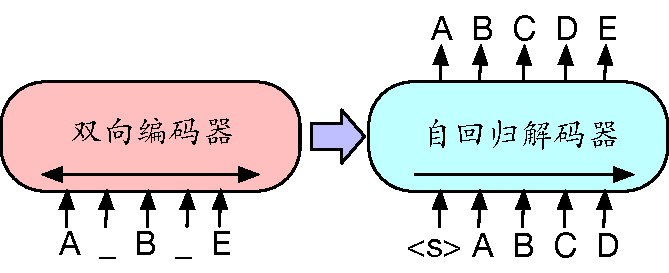
\includegraphics[scale=0.6]{\pref/bart.pdf}
    \caption{生成式语言模型BART的示意图.}
    \label{fig:autoencoder}
\end{figure}

我们已经指出,熵和编码有着密切的联系. 从这个角度出发,我们很容易理解生成模型背后的思想:我们希望通过训练的方式得到一个由神经网络所表示的编码和解码规则,他要尽可能符合真实数据的分布.

我们可以用一种非常简单的模型去理解这一过程. 假设所有的单词的集合为$\Sigma$,单词数为$k$的文本集合为$\Omega$. 我们希望训练一个生成模型$M$,给它输入$k-1$个单词,它可以给出第$k$个单词的概率分布,我们选择出现概率最大的那个词作为预测. 在训练的时候,对于一个句子$\omega$,我们只保留前$k-1$个词,得到$\omega[1:k]$,然后将它输入到生成模型$M$中,让它去预测第$k$个词. 

对于这一个具体的句子来说,理想的分布应该是一个\emph{Dirac分布}\index{Dirac分布}\footnote{Dirac分布是一个数学物理中更加常用的名字. 在概率论中,这也被称为\emph{退化分布}\index{退化分布};而在机器学习中,分布经常会表示为一个概率向量,文献中称为\emph{独热向量}\index{独热向量}. } $\delta_{\omega[k]}$,即以概率$1$取到$\omega[k]$. 假如说生成模型的输出是一个概率分布$M(\omega[1:k-1])=p$,那么,我们可以用K-L散度去衡量这两个分布的差异,因为$H(\delta_{\omega[k]})$是固定的,所以我们只考虑交叉熵$CH(\delta_{\omega[k]},p)$. 因为一次训练会给多个样本,所以我们的目标是同时最小化这些交叉熵的和. 假如训练集是$T$,我们的目标就是
\[
    \min_{M} \sum_{\omega\in T} CH(\delta_{\omega[k]},M(\omega[1:k-1])).
\]

实际上,这个例子是有普适性的,所有的监督训练的分类问题都可以用这种方式来建模. 而在 \Cref{???} 我们也会看到,此时交叉熵实际上被作为了一种\emph{损失函数}\index{损失函数}.

\section{附录:Shannon定理的证明}\label{sec:Shannon-thm-proofs}
我们在这一部分给出Shannon定理(\Cref{thm:Shannon-thm})的证明. 整体上的思路是:
\begin{enumerate}
    \item 证明如果$f$是单调函数,对正整数$m,n$成立$f(mn)=f(m)+f(n)$,那么$f(n)=C\log n$.
    \item 求出$H(1/n,\dots,1/n)$的表达式.
    \item 假设$p_i$是有理数,设$p_i=n_i/\sum_j n_j$,考虑$\sum_j n_j$个等可能试验结果,利用假设3推出$H$的表达式.
    \item 利用有理数的稠密性和$H$的连续性推出一般情形.
\end{enumerate}
最后一步是显然的,我们只需要证明前三步即可.

对第一步,我们需要证明的是,如果$f$是单调函数,对正整数$m,n$成立$f(mn)=f(m)+f(n)$,那么$f(n)=C\log n$. 首先,利用数学归纳法容易看出,对正整数$n,k$,成立
\begin{equation}
    f(n^k)=kf(n).\label{eq:Shannon-thm-proof-1}
\end{equation}

设$m,n$是任意两个大于$1$的整数,再选任意大的正整数$k$,从$m$进制数的性质可以看出,总存在正整数$l$使得
\begin{equation}
    m^l\leq n^k < m^{l+1}.\label{eq:Shannon-thm-proof-2}
\end{equation}
根据$f$的单调性,我们有
\[
    f(m^l)\leq f(n^k) < f(m^{l+1}).
\]
利用式 \eqref{eq:Shannon-thm-proof-1},我们有
\[
    lf(m)\leq kf(n) < (l+1)f(m)\iff \frac{l}{k}\leq \frac{f(n)}{f(m)} < \frac{l+1}{k}.
\]
将式 \eqref{eq:Shannon-thm-proof-2} 取对数,得到
\[
    l\log m\leq k\log n < (l+1)\log m\iff \frac{l}{k}\leq \frac{\log n}{\log m} < \frac{l+1}{k}.
\]
所以
\[
    \left|\frac{\log n}{\log m}-\frac{f(n)}{f(m)}\right|\leq\frac1k.
\]
因为$k$可以是任意大的正整数,取$k\to\infty$,我们就得到了
\[
    \frac{\log n}{\log m}=\frac{f(n)}{f(m)}.
\]
由$m,n$的任意性,取$m=2$,我们就得到了$f(n)=(f(2)/\log 2)\cdot \log n= C\log n$. 容易检验,$f(1)=0=C\log 1$,因此这一等式对所有正整数$n$都成立.

对第二步,我们需要求出$f(n)=H(1/n,\dots,1/n)$的表达式. 我们要利用第一步的结果,首先,根据假设二,$f(n)$是单调递增的函数. 然后,考虑$mn$个等可能试验,我们可以将它分成两步试验,第一步有$m$中等可能的结果,而在每一种结果之下,第二步有$n$种等可能结果. 根据假设三,
\[
f(mn)=f(m)+\frac{1}{n}\cdot nf(n)=f(m)+f(n).    
\]
所以$f(n)$符合第一步的假设. 第二步就可以直接从第一步推出.

最后,我们证明第三步. 设$p_1,\dots,p_n$都是有理数,那么,他们可以被写为
\[
    p_i=\frac{n_i}{\sum_{j=1}^n n_j}.
\]
其中$n_i$是非负整数. 我们考虑$\sum_j n_j$个等可能试验,这个试验可以被看成两步的试验,第一步有$n$种可能的结果,第$i$种结果出现的概率是$p_i$,而在第$i$种结果之下,第二步有$n_i$种等可能的结果. 根据假设三,和证明的第三步,我们有
\[
   C\log\sum_{j=1}^nn_j=H(p_1+\dots+p_n)+\sum_{i=1}^n p_i\cdot C\log n_i.
\]
因此,
\begin{align*}
    H(p_1,\dots,p_n)&=C\left(\log\sum_{j=1}^nn_j-\sum_{i=1}^n p_i\log n_i\right)\\
    &=C\left(\log\sum_{j=1}^nn_j-\sum_{i=1}^n p_i\log\left(p_i\sum_{j=1}^n n_j\right)\right)\\
    &=C\left(\log\sum_{j=1}^nn_j-\sum_{i=1}^n p_i\log p_i-\sum_{i=1}^n p_i\log\sum_{j=1}^n n_j\right)\\
    &=-C\sum_{i=1}^n p_i\log p_i.
\end{align*}
这正是我们要证明的. 于是,我们证明了Shannon定理.

\section{习题}
\begin{enumerate}[wide, labelindent=0pt]
    \item 我们在熵以及K-L散度的定义中,都规定了一些无定义的量的值,这些值并不是随便规定的,他们实际上反映了熵或者K-L散度定义中的连续性.
    \begin{enumerate}
        \item 证明:对给定的$a>0$,$\lim_{x\to 0+}x\log (x/a)=0$,因此我们规定了$0\log 0=0$以及$0\log(0/a)=0$.
        \item 证明:对给定的$a>0$,$\lim_{x\to 0+}x\log (a/x)=+\infty$,因此我们规定了$0\log(a/0)=+\infty$.
    \end{enumerate}
    
    \item 考虑关于$n$的正实数序列$a_1(n),\dots,a_k(n)$以及$b_1(n),\dots,b_k(n)$,假设对所有$i$,都成立$\lim_{n\to\infty} a_i(n)/b_i(n)=1$,证明:
    \[\lim_{n\to\infty}\frac{a_1(n)+\dots+a_k(n)}{b_1(n)+\dots+b_k(n)}=1.\]
    由此证明式 \eqref{eq:logP}.
    
    \item 证明\Cref{prop:entropy-2prob}.
    
    \item 用Lagrange乘子法重新证明\Cref{prop:entropy-maximum}.
    \begin{hint}
        如果你不知道Lagrange乘子法,可以参考 \Cref{???}.
    \end{hint}

    \item 证明\Cref{prop:conditional-mutual-information}.
    
    \item \cite{tingAmountInformation1962a} 仿照集合论的思路,我们可以定义三个随机变量的互信息为:
    \[I(X;Y;Z)=I(X;Y)-I(X;Y|Z).\]
    \begin{enumerate}
        \item 证明对称性:$I(X;Y;Z)=I(Y;X;Z) = I(X;Z;Y)$.
        \item 举一个例子说明,可能会有$I(X;Y;Z)<0$,所以这样定义的互信息并不一定真的代表“信息量”.
    \end{enumerate}

    \item 举一个例子说明,即便$D(p_1\Vert p_2)$很接近$0$,$D(p_2\Vert p_1)$也可能会很大.
    
    \item (\emph{单变量数据处理不等式})对任意离散随机变量$X$和函数$f$,证明:$H(X)\geq H(f(X))$.

    \item 考虑二分类的学习问题,此时对单个样本我们观察到的结果要么是$0$或$1$,假设在真实世界中样本总体服从参数为$\theta$的Bernoulli分布\index{Bernoulli分布},即$\Pr(X=1)=1-\Pr(X=0)=\theta$. 假设我们的数据集是$(x_1,y_1),\dots,(x_N,y_N)$,他们是从总体中独立采样得到的. 
    \begin{enumerate}
        \item 将问题考虑成一个数理统计问题,估计$\theta$. 写出似然函数\index{似然函数}$L(\theta;y_1,\dots,y_N)$.
        \item 再将问题考虑为一个信息论问题,写出每个样本的真实分布与估计分布之间的交叉熵之和$CH(\theta;y_1,\dots,y_N)$.
        \item 证明:$\max_{\theta} L(\theta;y_1,\dots,y_N)=\min_{\theta} CH(\theta;y_1,\dots,y_N)$,也就是说,\emph{最大似然估计等价于最小化交叉熵}.
    \end{enumerate}

    \item 请查找文献回答以下问题:
    \begin{enumerate}
        \item Fisher信息量是什么?它与K-L散度有什么样的关系?
        \item 列举其他概率分布之间散度的概念,他们是否是度量?
        \item 列举概率分布之间的度量,他们之间是否有关联?
    \end{enumerate}
    
\end{enumerate}
\section{章末注记}
信息一词的英文是“information”,从动词“inform”来,意思是告知、通知. 早在15世纪中叶,“information”一词的出现了义项“在通信中针对特定主题的知识”.\cite{InformationEtymologyOrigin} 这说明在那个时候人类就已经意识到,通信会产生新的东西,被称为知识或信息. 然而,人类对信息的严谨探索起步晚得多. 关于信息的物理学讨论源自统计力学,Boltzmann提出了著名的熵,证明了H定理,以此给出了热力学第二定律的微观解释. 关于Boltzmann的工作,参见 \cite{uffinkBoltzmannWorkStatistical2022}. 

一般认为,现代信息论的起源是Shannon的论文 \cite{shannonMathematicalTheoryCommunication1948},他在论文中提出了信息的数学定义,以及信息的基本性质. 但是,Shannon的工作并不是孤立的,他的工作是在统计力学的基础上发展起来的. 事实上,Shannon在论文中也提到了Boltzmann的熵. 这篇工作也被视为通信理论以及编码理论的奠基性工作.  Shannon在这篇论文中还给出了渐近意义下达到理论下界的最优编码,并且独立地被Fano \cite{robertm.fanoTransmissionInformation1949} 以一种不同的形式发现,因此后世称为Shannon-Fano编码. 但是Shannon-Fano编码并不是精确地达到下界,实际上,最优编码是Huffman \cite{huffmanMethodConstructionMinimumRedundancy1952} 给出的. Shannon在这篇论文中还讨论了渐近等分性,后来MciMillan的工作 \cite{mcmillanBasicTheoremsInformation1953} 和 Breiman的工作 \cite{breimanIndividualErgodicTheorem1957} 拓展了这一结果,因此后世称为Shannon-McMillan-Breiman定理. 

关于信息论与集合论的关系工作,可以参见Hu Kuo Ting的工作 \cite{tingAmountInformation1962a}. 他的工作还给出了多个随机变量互信息的定义,在这一章习题中有涉及.

相对熵的概念依然是从Shannon的奠基性论文 \cite{shannonMathematicalTheoryCommunication1948} 中提出的,但他只局限于通信的问题. 更加一般的讨论是由Kullback和Leibler在 \cite{kullbackInformationSufficiency1951} 给出,他们的是一种数理统计的思路,但是他们也具体地讨论了这一概念与信息的关系. 他们的论文中也讨论了交叉熵这一概念. 

机器学习中编码器和解码器的思路,最早是由Rumelhart,Hinton和Williams在 \cite{rumelhartLearningInternalRepresentations1986} 中提出,他们将编码器和解码器的整体称作\emph{自编码器}. 这篇工作几乎可以被视为深度学习的开山之作,它还提出了训练神经网络最常用的反向传播算法.

关于信息论的经典教科书,可以参见 \cite{coverElementsInformationTheory2012} ,此外,概率论的教材中也有很多很好的讨论,比如 \cite{jaynesProbabilityTheoryLogic2002},\cite{shiryaevProbability1996} 以及\cite{LiXianPingGaiLuLunJiChu2010}.

关于Kolmogorov复杂度的讨论,可以参见专著 \cite{???},这本书对于随机、信息、编码、复杂度,乃至归纳推理等概念都有非常独到的见解,值得一读. 

\endgroup
\chapter{差分隐私}\label{chap:differential-privacy}

在本章我们关心数据的另一个维度:社会属性. 机器学习需要大量的数据,这些数据从何而来?大部分时候,是通过收集个体的数据得到的. 于是这里就涉及到了隐私的问题,如何保护个体的隐私,同时又能够让机器学习得到足够的数据?\textbf{差分隐私}\index{差分隐私}就是解决这个问题的一个方法,本章将更详细地介绍差分隐私的概念和应用. 

\section{数据隐私问题}

许多科研工作的开展和推进都需要有大量真实有效的数据作为支撑. 以医学为例,我们需要大量真实的病人提供病情数据. 但这些数据可能都涉及到病人的隐私信息,例如一些\emph{敏感数据}. 因此,我们必须找到一种方法,既可以收集到这些数据,又保护病人的隐私信息.

保护病人的隐私信息的一种理解是不会让数据获得者将数据和人对应起来. 那么最直观的想法就是将每条\emph{数据匿名化}\index{数据匿名化}. 比如,每条数据只包含患者的生日、性别、邮政编号(代表位置)、病情. 这样做依然有问题:同一天生日、同一性别、相同邮政编号的人很少,而这些信息很容易被找到,比如公开的选民名册. 于是通过一条数据的各种属性可以轻易定位到这个人,这样的匿名化是不安全的.

我们再看一个例子。2006年,Netflix 举办了关于电影推荐系统的算法设计比赛.
只公开了匿名代号和对应用户的观看电影名称、打分的数据集(这次连生日、性别都没有). 但这一数据集很快被破解,问题出在只要对某个用户稍微熟悉一些,就很容易对应出这个用户和观影数据. 这种破解让部分用户感到焦虑,例如性少数群体害怕其他人可以从自己的观影记录中判断出自己的性取向. 第二届Netflix Prize 竞赛也因此停办.

这两个例子展现的是一种\emph{去匿名化}\index{去匿名化}的现象,也就是说匿名的数据实际上揭示了数据对应的那个个体。这去匿名化的出现都是因为数据具有\emph{独特性}. 比如我们看\Cref{tab:tab01},这是医院甲的病人数据表。56岁的病人只有Rebecca,所以假如我们知道Rebecca的年龄并了解到她去过这家医院,便立即得知她患有HIV.

\begin{table}[!ht]
\centering
\begin{tabular}{llllll}
    \toprule
    \textbf{Name} & \textbf{Age} & \textbf{Gender} & \textbf{Zip Code} & \textbf{Smoker} & \textbf{Diagnosis} \\ \midrule
    Richard & 64 & Male & 19146 & Y & Heart disease \\ 
    Susan & 61 & Female & 19118 & N & Arthritis \\ 
    Matthew & 67 & Male & 19104 & Y & Lung cancer \\ 
    Alice & 63 & Female & 19146 & N & Crohn's disease \\ 
    Thomas & 69 & Male & 19115 & Y & Lung cancer \\ 
    Rebecca & \textbf{56} & \textbf{Female} & 19103 & N & HIV \\ 
    Tony & 52 & Male & 19146 & Y & Lyme disease \\ 
    Mohammed & 59 & Male & 19130 & Y & Seasonal allergies \\ 
    Lisa & 55 & Female & 19146 & N & Ulcerative colitis \\ \bottomrule
\end{tabular}

\lhysays{改成中文版}
\caption{医院甲的病人数据表。}
\label{tab:tab01}
\end{table}

一种减少\emph{独特性}的思想是\emph{$k$-匿名性}\index{$k$-匿名性}:任何一个人的信息都不能和其他至少$(k-1)$人区分开. 比如,可以不明确写出姓名、年龄和邮编,只给出模糊的范围,于是数据变成了下面的\Cref{tab:tab02}.

\begin{table}[!ht]
\centering
\begin{tabular}{llllll}
\toprule
    \textbf{Name} & \textbf{Age} & \textbf{Gender} & \textbf{Zip Code} & \textbf{Smoker} & \textbf{Diagnosis} \\ \midrule
    * & 60-70 & Male & 191** & Y & Heart disease \\ 
    * & 60-70 & Female & 191** & N & Arthritis \\ 
    * & 60-70 & Male & 191** & Y & Lung cancer \\ 
    * & 60-70 & Female & 191** & N & Crohn's disease \\ 
    * & 60-70 & Male & 191** & Y & Lung cancer \\ 
    * & \textbf{50-60} & \textbf{Female} & 191** & N & HIV \\ 
    * & 50-60 & Male & 191** & Y & Lyme disease \\ 
    * & 50-60 & Male & 191** & Y & Seasonal allergies \\ 
    * & \textbf{50-60} & \textbf{Female} & 191** & N & Ulcerative colitis \\ \bottomrule
\end{tabular}

\lhysays{改成中文}
\caption{医院甲的病人数据表,模糊了姓名、年龄和邮编。}
\label{tab:tab02}
\end{table}

这种方法仍然存在问题,因为我们不能把关键信息(病症信息)也模糊化. 如果我们还拿到了另一家医院乙的模糊之后的病人数据表(\Cref{tab:tab03}),那么依然有办法定位到Rebecca:这两张表上50-60岁的女性只有HIV是重合的,如果我们知道Rebecca的年龄并知道她同时去过两家医院,便立即得知她患有HIV.

\begin{table}[!ht]
\centering
\begin{tabular}{lllll}
    \toprule
    \textbf{Name} & \textbf{Age} & \textbf{Gender} & \textbf{Zip Code} & \textbf{Diagnosis} \\\midrule
    * & \textbf{50-60} & \textbf{Female} & 191** & HIV \\ 
    * & \textbf{50-60} & \textbf{Female} & 191** & Lupus \\ 
    * & \textbf{50-60} & \textbf{Female} & 191** & Hip fracture \\ 
    * & 60-70 & Male & 191** & Pancreatic cancer \\ 
    * & 60-70 & Male & 191** & Ulcerative colitis \\ 
    * & 60-70 & Male & 191** & Flu-like symptoms \\ \bottomrule
\end{tabular}

\lhysays{改成中文}
\caption{医院乙的病人数据表,模糊了姓名、年龄和邮编。}
\label{tab:tab03}
\end{table}

除了使用匿名化的手段,还有一种方法可以保护隐私:不再提供单人的数据,而是直接公布将数据集的总体信息,比如平均值. 但这种方法也不一定能保证不泄露单人数据. 例如:我们只公布一个机器学习模型(这算是一直非常抽象的总体信息). 很多研究表明可以通过尝试不同的测试数据来判断出这个机器学习模型的训练集,这是因为机器学习模型总是会偏向于过拟合训练集数据. 所以如果对某个测试数据的结果很有自信,往往说明这一数据存在于训练集中. \lhysays{给一个ref}

\begin{remark}
以上这些内容都说明\textbf{匿名化}很难保护个人隐私. 那么是否可以使用密码学的手段进行\textbf{加密}?其实加密和隐私在出发点上完全不同. 加密的目的是为了不让别人获取到真实数据. 而隐私是一个比简单地锁定数据更微妙的问题——我们希望我们的算法的结果能够释放有用的信息,而不是泄露私人信息. 因此我们这里讨论的其实是隐私保护问题而不是加密问题。
\end{remark}

\section{差分隐私的定义与性质}

我们上面探讨了隐私保护的必要性以及它的微妙之处,现在我们要给出一种合理的方案解决隐私保护的问题,这个方案就是\emph{差分隐私}。要给出一个数学模型,不仅要知道什么情况下算是隐私泄漏,也需要知道什么情况下不算,所以我们再来看一个反面的例子。

Broky是一位长期吸烟的男子,他参加了一项有关“吸烟与健康”的调查. 这项调查在不久后发布了一项结果,表明长期吸烟的人患上肺癌的几率更大. 伴随着这一结果的公布,保险公司在出售相同保险时会对长期吸烟者索要更高的价格. Broky当然也受到了这一政策的影响. 那我们是否可以认为这项研究泄露了Broky(更有可能患病)的隐私呢?

我们的直观应该是不算泄露了隐私. 因为“长期吸烟的人患上肺癌的几率更大”这项结论并不依赖于Broky是否参加了调查. 考虑这样的对照,$x$代表原来参加调查的人的集合,$x'$代表其他人不变,只是Broky换成了另外一个人的集合. 如果是$x'$这些人参与了调查,结论是否会发生变化?\emph{大概率}不会!

Broky的例子告诉我们对于隐私的一种合理的衡量应该有以下性质:\emph{当数据集中包含Broky的信息,相比数据集中不包含Broky的信息,并不会\textbf{明显}增加损害Broky的利益的概率.} 这一思想引出了\emph{差分隐私}\index{差分隐私}的概念,我们将在下面给出数学形式的定义.

考虑数据的空间$\mathcal X$,其中的每一个元素都包含了个体的所有可能数据例如姓名、性别、年龄、国籍等. 考虑$n$个人的数据,形成了有序的数据集$x = (x_1, \cdots, x_n) \in \mathcal X^n$.  设 $A$ 是一种随机算法:在固定输入数据集 $x \in \mathcal X^n$下,$A(x)$ 是结果空间 $\mathcal Y$ 上的一个随机变量. 当我们改变(增加或删除)一个人的数据时,我们希望结果分布的变化可以控制在一定范围内. 为此,我们引入相邻数据集的概念:

\begin{definition}[$k$-相邻数据集]\index{$k$-相邻数据集}
    设 $x, x' \in \mathcal X^n$,如果 $x$ 和 $x'$ 最多有$k$条数据不同,即至多存在$k$个不同的$i_1,\dots,i_k \in [n]$ 使得 $x_{i_j}=x_{i_j}'$对$j\in[k]$成立,那么称 $x$ 和 $x'$ 是 $k$-相邻的.
\end{definition}

在之前的例子中,含有Broky的被调查者的数据集和把Broky换为任意一个其他人的数据集时$1$-相邻数据集.

现在我们给出差分隐私的定义。

\begin{definition}[$\epsilon$-DP]\index{$\epsilon$-DP}
考虑随机算法 $A : \mathcal X^n \to \mathcal Y$,如果对于任一对$1$-相邻数据集$x, x'$,对任意(可测)值集 $E \subseteq \mathcal Y$,有
\[
\Pr(A(x)\in E) \leq e^{\epsilon} \cdot \Pr(A(x')\in E),
\]
那么我们称$A$为\emph{数据集大小为 $n$ 的 $\epsilon$-DP算法}.
\end{definition}

需要注意的是,这一定义是针对随机算法的,并且是对称的,也就是$x$和$x'$的地位是平等的。直观上一个,$\epsilon$-DP算法的输出分布在相邻数据集上的变化不会太大. $\epsilon$衡量的是信息的泄漏量;$\epsilon$越大,算法泄漏的信息就越多,隐私保护效果当然也变差.

以上定义需要对所有的(可测)值集$E$都成立,这给验证带来了极大的困难,如果随机算法的输出分布是更加常规的,我们可以简化验证的过程. 

对于离散型的输出,我们有如下等价定义:
\begin{proposition}\label{prop:discrete-dp}
    如果 $A(x)$对于任意 $x \in \mathcal X^n$ 都是离散型随机变量,那么随机算法$A$是数据集大小为 $n$ 的 $\epsilon$-DP算法,当且仅当对于任意一对$1$-相邻数据集$x, x'$和所有的 $y \in \mathcal Y$,有
    \[
    \Pr(A(x) = y) \leq e^{\epsilon} \cdot \Pr(A(x') = y).
    \]
\end{proposition}
\begin{proof}
$\implies$:取$E = \{y\}$即可证明.

$\impliedby$:假设$E=\{y_1,\dots,y_k,\dots\}$. 对每一个$y_i$,都有
    \[
    \Pr(A(x) = y_i) \leq e^{\epsilon} \cdot \Pr(A(x') = y_i).
    \]
因为$A(\cdot)=y_i$对于不同的$i$是互斥事件,所以概率可以直接相加,于是:
    \[
    \Pr(A(x) \in E) = \sum_i \Pr(A(x) = y_i) \leq e^{\epsilon} \cdot \sum_i\Pr(A(x') = y_i) = e^{\epsilon} \cdot \Pr(A(x') \in E).
    \]
\end{proof}

对连续型的输出,我们有如下等价定义:
\begin{proposition}\label{prop:continuous-dp}
如果 $A(x)$对于任意 $x \in \mathcal X^n$ 都是连续型随机变量,那么它存在概率密度函数,记为$h_{x}$. 此时随机算法$A$是数据集大小为 $n$ 的 $\epsilon$-DP算法,当且仅当对于任意一对$1$-相邻数据集$x, x'$和几乎所有的 $y \in \mathcal Y$,有
    \[
    h_{x}(y) \leq e^{\epsilon} \cdot h_{x'}(y).
    \]
\end{proposition}
\begin{proof}\footnote{这一部分的严格表述需要测度论的基础,所以这一证明从直观上理解即可,不需要考虑严格的定义。}
$\implies$:根据概率密度函数的定义(实际上是Lebesgue微分定理),对$x\in\mathcal X^n$,取$E_\delta = (y-\delta, y+\delta)$,对几乎所有的$y\in\mathcal Y$,有
\[\frac{\d}{\d\delta}\Pr(A(x)\in E_\delta)=h_x(y).\]
因此,对几乎所有的$y\in\mathcal Y$,
\[\forall\delta>0\,\Pr(A(x)\in E_\delta) \leq e^{\epsilon} \cdot \Pr(A(x')\in E_\delta)\implies h_x(y)\leq e^\epsilon\cdot h_{x'}(y).\]
$\impliedby$:依然根据概率密度函数的定义,考虑$x,x'\in\mathcal X^n$,对任意可测$E\subseteq\mathcal Y$,有
\[\Pr(A(x)\in E)=\int_E h_x(y)\d y\leq e^\epsilon\cdot\int_E h_{x'}(y)\d y=e^\epsilon\cdot\Pr(A(x')\in E).\]
\end{proof}

接下来我们给出差分隐私的基本性质。

\begin{proposition}[复合性,两个算法的情形]\label{prop:composition}\index{差分隐私!复合性}
    $A_1$ 和 $A_2$ 是相互独立的随机算法,其中 $A_1 : X^n \to \mathcal Y_1$,$A_2 : \mathcal Y_1 \times \mathcal X^n \to \mathcal Y_2$. 假设$A_1$是 $\epsilon_1$-DP算法,$A_2$ 是 $\epsilon_2$-DP算法.
    
    令 $A :\mathcal X^n \to \mathcal Y_1 \times \mathcal Y_2$ 是随机算法,输出为 $A(x) = (y_1, y_2)$,其中 $y_1 = A_1(x)$, $y_2 = A_2(y_1, x)$,那么 A 是$(\epsilon_1 + \epsilon_2)$-DP算法.
\end{proposition}

\begin{proof}
为了简化记号,这里我们只证明离散的情况. 令 $x,x'$ 是 $\mathcal X^n$ 中的两个$1$-相邻数据集,$A$输出为 $y = (y_1, y_2) \in \mathcal Y_1 \times \mathcal Y_2$,那么根据定义和独立性,
    \[
    \Pr(A(x) = (y_1, y_2)) = \Pr(A_1(x) = y_1) \cdot \Pr(A_2(y_1, x) = y_2).
    \]
由于 $A_1$ 是 $\epsilon_1$-DP算法,$A_2$是 $\epsilon_2$-DP算法,得到
    \[
    \begin{aligned}
        \Pr(A(x) = (y_1, y_2)) &= \Pr(A_1(x) = y_1) \cdot \Pr(A_2(y_1, x) = y_2)\\
        &\leq e^{\epsilon_1} \Pr(A_1(x') = y_1) \cdot e^{\epsilon_2} \Pr(A_2(y_1, x') = y_2) \\
        &= e^{\epsilon_1 + \epsilon_2} \cdot \Pr(A(x') = (y_1, y_2)).
    \end{aligned}
    \]
\end{proof}

利用数学归纳法,很容易推广到多个随机算法的复合性:

\begin{proposition}[复合性,多个算法的情形]\label{prop:composition-multi}\index{差分隐私!复合性}
    设 $A_1, A_2, \cdots , A_k$ 为一列相互独立的随机算法, 
    \begin{align*}
        A_1&: \mathcal X^n \to \mathcal Y_1,\\
        A_i&: \mathcal Y_1 \times \cdots \times \mathcal Y_{i-1} \times \mathcal X^n \to \mathcal Y_i,\quad i = 2, 3, \cdots, k.
    \end{align*}
    也就是 $A_i$ 将 $A_1, \cdots, A_{i-1}$ 的输出和 $\mathcal X^n$ 中的一个数据集作为输入元素. 对$i=1,\dots,k$, $A_i$是 $\epsilon_i$-DP算法. 
        
    依次运行算法 $A_i$ 得到算法$A : \mathcal X^n \to \mathcal Y_1 \times \cdots \times \mathcal Y_k$,那么$A$是$\epsilon$-DP,其中$\epsilon = \sum_{i=1}^n \epsilon_i$.
\end{proposition}

接下来的性质是说明操纵随机算法的输出不会影响隐私保护的效果:

\begin{proposition}[后处理]\label{prop:post-processing}\index{差分隐私!后处理}
    令 $A : \mathcal X^n \to \mathcal Y$, $B : \mathcal Y \to \mathcal Z$ 为相互独立的随机算法,其中 $\mathcal X$, $\mathcal Y$, $\mathcal Z$ 是任意集合. 如果 $A$ 是 $\epsilon$-DP算法,那么组合算法$ B(A(\cdot))$ 也是 $\epsilon$-DP算法.
\end{proposition}
\begin{proof}
我们仍然只考虑离散情形,采用定义的方法证明
    \[
    \begin{aligned}
        \Pr(B(A(x)) = b) &= \sum_{y \in \mathcal Y} \Pr(A(x) = y) \Pr(B(y) = b) \\
        &\leq e^{\epsilon} \sum_{y\in \mathcal Y}\Pr(A(x') = y)\Pr(B(y) = b)\\
        &= e^{\epsilon}\Pr(B(A(x')) = b).
    \end{aligned}
    \]
\end{proof}

最后,我们讨论如果有多个人的数据都发生变化的时候,隐私保护的性质会发生什么变化。

\begin{proposition}[群体隐私]\label{prop:group-privacy}\index{差分隐私!群体隐私}
    令 $x, x' \in \mathcal X^n$ 是$k$-相邻数据集,$1 \leq k \leq n$. 如果 $A$ 是 $\epsilon$-DP算法,那么对所有的值集$E$,我们有
    \[
    \Pr(A(x) \in E) \leq e^{k\epsilon}\Pr(A(x') \in E).
    \]
\end{proposition}
\begin{proof}
    考虑数据集 $x_0, x_1, \cdots , x_k$,其中 $x_0 = x$, $x_k = x'$,且 $x_i$ 和 $x_{i+1}$ 是$1$-相邻数据集,$i = 0, \cdots, k-1$. 那么
    \[
    \begin{aligned}
    \Pr(A(x) \in E) &\leq e^{\epsilon}\Pr(A(x_1) \in E) \leq e^{2\epsilon}\Pr(A(x_2) \in E)\\
    &\leq \cdots \leq e^{k\epsilon}\Pr(A(x') \in E).
    \end{aligned}
    \]
\end{proof}

换言之,$k$-相邻数据集上$\epsilon$-DP算法的表现仿佛一个$k\epsilon$-DP算法。

这一性质还可以推出$\epsilon$的含义。我们知道数据集$x, x' \in \mathcal X^n$最多在$n$个位置不同. 所以对于一个$\epsilon$-DP算法$A$,一定有
        \[
        \Pr(A(x) \in E) \leq e^{n\epsilon}\Pr(A(x') \in E).
        \]
如果这里的$\epsilon$太小,意味着这一算法对任何输入都有相似的输出. 换句话说,算法压根没有输出任何有意义的内容. 于是,我们更定量说明了,$\epsilon$还代表信息的泄露量. 因此,一个实用的DP算法不能让$\epsilon$太小,否则输出没有意义;也不能让$\epsilon$太大,否则隐私保护效果不好.

\section{差分隐私的应用}
在这一部分,我们将会具体讨论三个差分隐私的算法。

\subsection{随机反应算法}
我们从一个具体场景开始。假设有一名老师想要调查班上的同学有多少人曾经在考试中作弊. 设班上一共有$n$名同学,每个人回答一个数字$x_i \in \{0,1\}$. 对于每个$i$,独立地按照以下规则根据$x_i$得到对应的$y_i$:
\[\begin{aligned}
    y_i =
    \begin{cases}
        x_i, & \text{ 以$2/3$的概率 }, \\
        1 - x_i,& \text{ 以$1/3$的概率}.
    \end{cases}
\end{aligned}\]
并输出$\sum_{i=1}^n y_i$. 

我们称这一算法为\emph{随机反应}(RR)算法\index{随机反应算法}\index{RR算法}. 当$y_i = 1$时,学生$i$可以声称这是由于算法的随机机制造成的,而并非自己真的作弊过.

RR算法在隐私保护上的表现由以下定理给出:
\begin{theorem}
    RR 算法是 $\log 2$-DP算法.
\end{theorem}
\begin{proof}
记$Y_i$是$y_i$对应的随机变量. 我们知道$y_i$之间相互独立,所以
    \[
    \Pr(A(x) = y) = \prod_{i=1}^n \Pr(Y_i = y_i \mid x_i).
    \]
对于$y_i$,我们有
    \[
    \frac{\Pr(Y_i = y_i \mid x_i = y_i)}{\Pr(Y_i = y_i \mid x_i = 1 - y_i)} = \frac{2/3}{1/3} = 2.
    \]
所以对于一对$1$-相邻数据集$x, x'$和任意的$y \in \mathcal Y$,假设$x_j \neq x'_j$,有
    \[
    \frac12 \leq \frac{\Pr(A(x) = y)}{\Pr(A(x') = y)} = \frac{\prod_{i=1}^n \Pr(Y_i = y_i \mid x_i)}{\prod_{i=1}^n \Pr(Y_i = y_i \mid x'_i)} = \frac{\Pr(Y_j = y_j \mid x_j)}{\Pr(Y_j = y_j \mid x'_j)} \leq 2.
    \]
由定义,RR 算法是 $\log 2$-DP算法.
\end{proof}

另一方面,我们还关注RR算法得到的$\sum_{i=1}^n y_i$是否能很好的估计出$\sum_{i=1}^n x_i$. 为此,假设随机变量$X_1, \cdots, X_n$独立服从参数为$p$的Bernoulli分布,即 $\Pr(X_i=1) =p$ 而 $\Pr(X_i=0)= 1-p$. 于是,
\[\begin{aligned}
    q = \Pr(Y_i = 1) &= p \cdot \frac23 + (1 - p) \cdot \frac13 \\
    \implies p &= 3 q - 1.   
\end{aligned}\]
我们得到的$\sum_{i=1}^n y_i$相当于是$q$,真正的参数$p$和$q$存在上述关系. 设$\hat{X} = \sum_{i=1}^n (3 Y_i - 1)$,可得$\E[\hat{X}] = \E[\sum_{i=1}^n X_i]$.

\subsection{全局灵敏度与Laplace机制}
从RR算法中获得灵感,我们可以在算法中添加随机性,比如向算法$f$的输出添加噪声. 那么就引出了另一个问题,需要添加多大的噪声?这和算法本身的性质有关,比如,当输入只改变一点时,算法的输出会改变多大?我们定义全局灵敏度来衡量这一性质.

\begin{definition}[全局灵敏度]\index{全局灵敏度}
给定算法$f: \mathcal X^n \to \R$,定义$f$的\textbf{全局灵敏度}为
    \[
    \mathsf{GS}_f = \sup_{x, x' \text{ 在 }\mathcal X^n\text{ $1$-相邻}} |f(x) - f(x')|. 
    \]
\end{definition}
定义中的$1$-相邻,可能会随着情景不同而改变. 全局灵敏度的定义是很直观的,就是改变一条数据会对算法输出带来的最大可能变化。

我们来计算一个简单的例子.
\begin{example}
设$f(x)= \frac1n \sum_{i=1}^n \phi(x_i)$,$\phi : \mathcal X\to [0,1]$是满射. 那么,
\begin{align*}
    \mathsf{GS}_f&=\sup_{x, x' \text{ 在 }\mathcal X^n\text{ $1$-相邻}} |f(x) - f(x')|\\
    &= \sup_{x, x' \text{ 在 }\mathcal X^n\text{ $1$-相邻}} \frac1n \left|\sum_{i=1}^n \phi(x_i) - \sum_{i=1}^n \phi(x'_i)\right|\\
    &= \sup_{x, x' \text{ 在 }\mathcal X^n\text{ 只在 } j\text{ 不同}} \frac1n \left|\phi(x_j) - \phi(x'_j)\right| = \frac1n.
\end{align*}
\end{example}

利用全局灵敏度的概念,我们实际上有一个一般的方法来构造差分隐私算法. 我们称这一方法为\emph{Laplace机制}\index{Laplace机制}. 首先引入Laplace分布的概念.

\begin{definition}[Laplace分布]\index{Laplace分布}
    给定参数$\mu\in\R$和$\lambda>0$,定义概率密度函数
        \[h(x \mid \mu, \lambda) = \frac1{2\lambda}\exp\left(- \frac{|x - \mu|}{\lambda}\right).\]
我们称具有这一密度的分布为\emph{Laplace分布},记为$\mathsf{Lap}(\mu,\lambda)$.
\end{definition}

Laplace分布是服从双边指数分布的随机变量进行线性变换后服从的分布. 具体来说,设$X\sim\mathsf{DExp}(1)$,那么$\lambda X+\mu\sim\mathsf{Lap}(\mu,\lambda)$. 在\Cref{fig:Laplace-distribution} 中,我们展示了不同参数的Laplace分布密度函数图像。更多关于Laplace分布的性质,我们留做习题. \lhysays{习题}

\begin{figure}[ht]
    \centering
    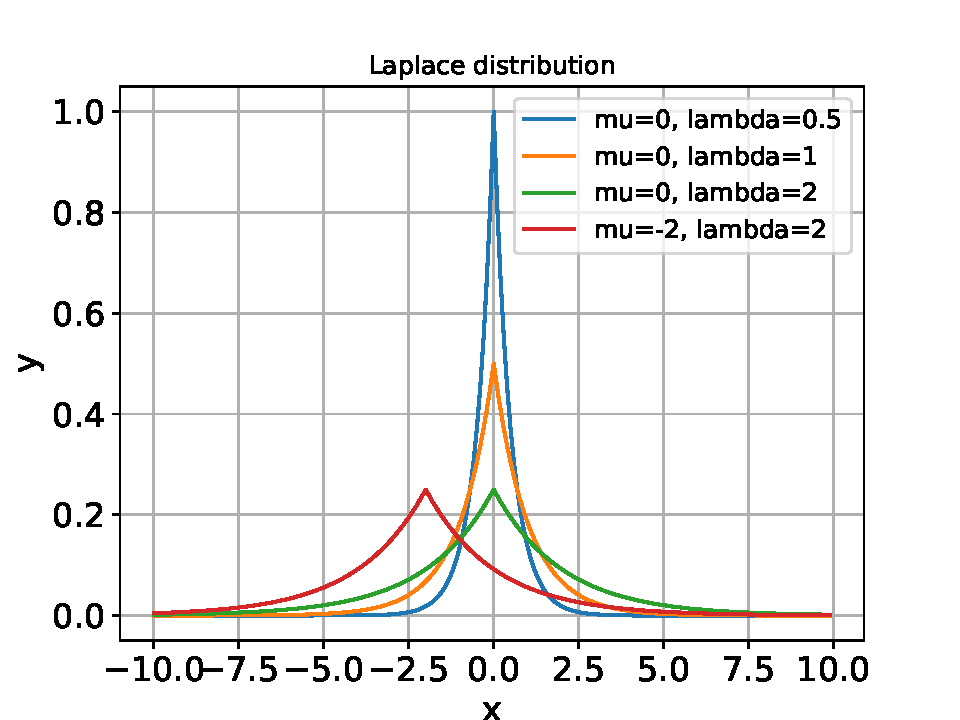
\includegraphics[scale=0.6]{Chapters/differential-privacy/figures/LaplaceDist.pdf}
    \caption{Laplace分布的密度函数图像}
    \label{fig:Laplace-distribution}
\end{figure}

下面我们来陈述Laplace机制。我们想利用Laplace分布来创造一些随机性. 给定一个数据集$x \in \mathcal X^n$ 和参数$\epsilon$. 对于一个算法$f:\mathcal X^n \to \R$,先计算出$f$的全局灵敏度$\mathsf{GS}_f$。输出$A_{\mathsf{Lap}}(\epsilon, x) = f(x) + Z$,其中$Z\sim \mathsf{Lap}(0, \mathsf{GS}_f/\epsilon)$. 将随机算法$A_{\mathsf{Lap}}(\epsilon, \cdot)$称为\emph{Laplace机制}\index{Laplace机制}。我们有以下定理:
\begin{theorem}\label{thm:laplace-mechanism}
    对于任意的$\epsilon > 0$,Laplace机制是$\epsilon$-DP算法.
\end{theorem}
\begin{proof}
设$x$,$x'$是两个$1$-相邻数据集,记$\mu = f(x)$,$\mu' = f(x')$. 由Laplace分布的性质可知,$A_{\mathsf{Lap}}(\epsilon, x) \sim \mathsf{Lap}(\mu, GS_f/\epsilon)$,$A_{\mathsf{Lap}}(\epsilon, x') \sim \mathsf{Lap}(\mu', GS_f/\epsilon)$.

因此,对于任意的$y \in \mathcal Y$,有
    \[
    \begin{aligned}
        \frac{h_{x}(y)}{h_{x'}(y)} &=\exp \left(-\epsilon \frac{|\mu - y| - |\mu' - y|}{GS_f} \right) \\
        &\leq \exp \left(\epsilon \frac{|\mu - \mu'|}{GS_f} \right)\leq \exp(\epsilon).
    \end{aligned}
    \]
根据\Cref{prop:continuous-dp},命题得证。
\end{proof}

\subsection{DP版本Llyod算法}
作为一个Laplace机制的具体实例,我们将$k$-均值聚类问题的经典算法Llyod算法改造成一个差分隐私算法.

\emph{$k$-均值}\index{$k$-均值}聚类问题指的是给定一个数据集$x$,找到$k$个点(中心)$\{c_i\} \subseteq \R^d$,使得$\sum_{i \in [n]} \min_{j\in[k]} \norm{x_i - c_j}^2$最小. 通俗来说,就是找到$k$个中心,使得数据集中每个点到最近的中心的距离之和最小. $k$-均值问题最常见的解决方法是使用迭代的启发式的\emph{Lloyd算法}\index{Lloyd算法},其表述为下:\lhysays{改成算法模板}
\begin{itemize}
    \item 输入:数据集$x \in \mathcal X^n$,这里$\mathcal X = \{x \in \R^d : \norm{x}_1 \leq 1 \}$,参数$k$.
    \item 随机初始化$c_1^{(0)}$, $c_2^{(0)}$, $\cdots$, $c_k^{(0)} \in \mathcal X$.
    \item for $t=1$ to $T$
    \begin{itemize}
        \item for $j=1$ to k
        \begin{itemize}
            \item 计算$S_j = \{i : c_{j}^{(t-1)} \text{ 是\ } x_i \text{ 最近的中心}\}$.
            \item 更新$c_j^{(t)} = \frac1{|S_j|}\sum_{i\in S_j} x_i$.
        \end{itemize}
    \end{itemize}
    \item 输出:$c_1^{(T)}$, $c_2^{(T)}$, $\cdots$, $c_k^{(T)}$.
\end{itemize}

这个算法可以达到很好的效果,但它并不能保证DP性质. 我们希望对这一算法进行小规模的修改,让它具有$\epsilon$-DP的性质. 我们给出如下的DP版本Llyod算法. \lhysays{改成算法模板}

\begin{itemize}
    \item 输入:数据集$x \in \mathcal X^n$,这里$\mathcal X = \{x \in \R^d : ||x||_1 \leq 1 \}$,参数$k$,\textcolor{red}{参数$\epsilon$}.
    \item \textcolor{red}{$\epsilon' = \frac{\epsilon}{2 T}$},随机初始化$c_1^{(0)}$, $c_2^{(0)}$, $\cdots$, $c_k^{(0)} \in \mathcal X$.
    \item for $t=1$ to $T$
    \begin{itemize}
        \item for $j=1$ to k
        \begin{itemize}
            \item 计算$S_j = \{i : c_{j}^{(t-1)} \text{ 是 } x_i \text{ 最近的中心}\}$.
            \item $n_j = |S_j|$.
            \item $a_j = \sum_{i\in S_j} x_i$.
            \item \textcolor{red}{计算 $\hat{n_j} = n_j + Y$,$Y \sim \mathsf{Lap}(0, 2/\epsilon')$.}
            \item \textcolor{red}{计算 $\hat{a_j} = a_j + (Z_1, \cdots, Z_d)$,$Z_i \text{ i.i.d.}\sim \mathsf{Lap}(0, 2/\epsilon')$.}
            \item 更新
            $\begin{aligned}
            c_j^{(t)} =
            \begin{cases}
                \textcolor{red}{\frac{\hat{a_j}}{\hat{n_j}}}, & \hat{n_j} \geq 1, \\
                \mathcal X\text{ 上的一个随机均匀采样}, & \hat{n_j} < 1.
            \end{cases}
            \end{aligned}$
        \end{itemize}
    \end{itemize}
    \item 输出:$c_1^{(T)}$, $c_2^{(T)}$, $\cdots$, $c_k^{(T)}$.
\end{itemize}

以下定理表明上面的算法确实是一个$\epsilon$-DP算法。
\begin{theorem}
    DP 版本的 Lloyd算法是$\epsilon$-DP算法.
\end{theorem}

\begin{proof}[证明概要]
我们只在这里陈述证明的大致想法,将细节留到习题\lhysays{习题}.

在第一步中,我们设置了$\epsilon' = \epsilon / 2 T$. 我们把整体的算法拆成$T$个阶段,其中第$t$轮迭代$A_t$以$c_1^{(t-1)},c_2^{(t-1)},\dots,c_k^{(t-1)}$作为输入,输出$c_1^{(t)},c_2^{(t)},\dots,c_k^{(t)}$. 如果可以得到$A_t$是$2 \epsilon'$-DP算法,那么由DP算法的复合性,就可以得到整个算法是$T \cdot 2\epsilon'$-DP,也就是$\epsilon$-DP.

进一步,考虑证明每一个$A_t$是$2 \epsilon'$-DP算法. 将$A_t$内循环的每一轮(以$j$为变量)视为输入为$n_j,a_j$,输出为$\hat{n}_j$,$\hat{a}_j$的算法. 分别证明这些算法符合$2\epsilon'$-DP,然后再次借助DP算法的复合性.
\end{proof}

\section{差分隐私与信息论}
\lhysays{讨论信息论约束下的差分隐私问题}

\section{习题}

\section{章末注记}

\part{决策与优化}\label{part:decision-optimization}
\chapter{凸分析}\label{chap:convex-analysis}

本章将会建立关于决策与优化的基本理论,这些方法论都是数据驱动的机器学习的基础,他们涉及从数据到建立模型的步骤(即训练). 优化与分析有着密不可分的联系,所以本章我们会立足优化问题的一些基本事实,建立凸分析理论。凸分析是优化理论的基础.

\section{决策与优化的基本原理}
\subsection{统计决策理论}\index{统计决策理论}
\lhysays{这部分要细化}

我们在前一部分讨论过,数据(或者说信息)的意义总是体现在集合的对象中,我们把我们所关心的集合对象称为(随机)\emph{总体}\index{总体} $P$。从概率论角度看,总体就是一个概率分布。现在我们从总体$P$中抽取一个\emph{样本}\index{样本} $X$。这件事情在概率论上意味着我们得到了一个随机变量$X$服从分布$P$。拿到样本之后,我们的任务是做出\emph{好的决策},因此,决策$T$是一个依赖$X$的函数. 比如说,$P$是所有大学生的身高,$X$是随机抽选一个人测量的身高,我们的决策$T$是估计大学生的平均身高。

“好的决策”指的是函数$T$能够具备某些量化指标. 其中非常常用的一个方法是通过\emph{损失函数}\index{损失函数}来衡量,它是总体$P$和决策$T(X)$的函数,即$L(P,T(X))$. 损失函数在不同语境下有不同称呼。例如,在经济学和金融学的风险理论中,损失函数被称为\emph{风险函数}\index{风险函数},它意味着个体在面对不确定的环境下所需要面对的风险。而在优化理论中,损失函数往往被称为\emph{目标函数}\index{目标函数},表明所要优化的对象。

决策$T$的一种量化指标是最小化期望意义下的损失函数:
    \[\min_{T}\E_{X\sim P}(L(P,T(X))).\]
在经济学中,这一量化指标实际上是von Neumann和Morgenstern \emph{期望效用理论}\index{期望效用理论}的具体体现。这一理论认为,个体在面对不确定的环境时,会选择最大化期望效用的决策;在风险理论的语境下,则是最小化期望风险的的决策。

现在我们考虑一个非常一般的决策任务。假设我们的任务是估计函数$f$,但是我们只知道观测到的自变量$X$(来自总体$P$)以及它的函数值$Y=f(X)$,我们的决策是函数的估计值$\hat f$. 在机器学习中,$f$通常是需要训练的模型. 我们可以写出若干种损失函数:
\begin{itemize}
    \item 平方($L^2$)损失函数\index{损失函数!平方~}\index{损失函数!$L^2$~}:$L(P,T(X))=(Y-\hat f(X))^2$. 使用此损失函数的时候,我们要假定$f$在实数范围取值。
    \item $L^1$损失函数\index{损失函数!$L^1$~}:$L(P,T(X))=|Y-\hat f(X)|$. 使用此损失函数的时候,我们要假定$f$在实数范围取值。
    \item SVM损失函数(hinge损失函数)\index{损失函数!SVM~}\index{损失函数!hinge~}:$L(P,T(X))=\max\{0,1-Y\cdot\hat f(X)\}$. 使用此损失函数的时候,我们一般要假定$f(X)\in[-1,1]$。
    \item 交叉熵损失函数\index{损失函数!交叉熵~}:$L(P,T(X))=CH(\hat f(X),Y)$.
\end{itemize}

这些损失函数会用在不同的场景之中。通常来说,机器学习中有两类问题:\emph{回归问题}\index{回归问题}和\emph{分类问题}\index{分类问题}和。他们两个的区别主要在于回归问题中$f$取值为实数,而且通常随自变量连续变化;而分类问题中$f$只取有限多个值,他们通常被作为标签(比如这张图片是人还是青蛙)使用。在回归问题中,我们通常使用平方损失函数或者$L^1$损失函数;在分类问题中,我们通常使用SVM损失函数或者交叉熵损失函数。

\subsection{优化问题}\index{优化问题}
现在我们从决策过渡到优化。在最简单的决策问题中,我们的目标就是找到某个$x$使得(期望)损失函数$f$最小. 此时,问题的一般形式为:
\begin{alignat*}{2}
\min_{x}&\quad f(x)\\
\text{s.t.}&\quad f_i(x)=0,&\quad i=1,\dots,m,\\
&\quad g_j(x)\leq 0,&\quad j=1,\dots,n,\\
&\quad x\in\Omega.
\end{alignat*}
这里,s.t(subject to)之后的内容表明了$x$取值的限制,因此被称为\emph{约束}\index{约束}. 其中$f_i(x)=0$和$g_j(x)\leq 0$被称为\emph{函数约束}\index{约束!函数~},而$x\in\Omega$被称为\emph{集合约束}\index{约束!集合~}.

优化的基本任务就是找到$x$最小化损失函数. 

根据损失函数$f$、约束条件$f_i$和$g_j$的不同性质,我们可以对优化问题进行分类:
\begin{itemize}
\item 无约束优化\index{优化问题!无约束优化}:约束条件$f_i$和$g_j$实际上不存在,即$m=n=0$,并且$\Omega$是全空间,比如$\R^n$.
\item 有约束优化\index{优化问题!有约束优化}:至少存在一个约束条件,即$\min\{m,n\}\geq 1$,或者$\Omega$不是全空间。
\item 光滑优化\index{优化问题!光滑优化}:损失函数和约束条件都是可微函数.\footnote{光滑这一词的含义在不同的文献中大相径庭,它可以指(连续)可微、连续可微、二次(连续)可微或者无穷次可微。}
\item 线性优化\index{优化问题!线性优化}:损失函数和约束条件都是线性函数(形如$a^\t x+b$).
\end{itemize}

\begin{remark}
    \lhysays{介绍一下控制理论与优化理论的异同,特别是连续控制和随机优化。}
\end{remark}

下面我们看几个经典的优化例子。
\begin{example}[最小二乘法]\label{ex:least-square}\index{最小二乘法}
    给定矩阵$A\in\R^{m\times n}$和向量$b\in\R^m$,考虑如下优化问题:
    \begin{alignat*}{2}
    \min_{x}&\quad \norm{Ax-b}_2^2\\
    \text{s.t.}&\quad x\in\R^n.
    \end{alignat*}
    这个问题被称为\textbf{最小二乘法}\index{最小二乘法}. 目标函数可以被写为$(Ax-b)^\t(Ax-b)$,因此最小二乘法是一种典型的无约束光滑优化问题。

    最小二乘法的解$x^*$实际上是\emph{投影}\index{投影}解:$b$的行向量投影到$A$的列向量形成的线性空间,正好是$Ax^*$. \lhysays{加个图,补全细节} 因此,求投影也可以被写作一个优化问题.
\end{example}

\begin{example}[线性规划]\label{ex:linear-programming}\index{线性规划}
    给定矩阵$A\in\R^{m\times n}$和向量$b\in\R^m$,考虑如下优化问题:
    \begin{alignat*}{2}
    \min_{x}&\quad c^\t x\\
    \text{s.t.}&\quad Ax\leq b,\\
    &\quad x\geq 0.
    \end{alignat*}
    这个问题被称为\textbf{线性规划}\index{线性规划}. 目标函数和约束条件都是线性的,因此线性规划是一种典型的线性优化问题. \lhysays{加个图,补全细节}
\end{example}

上面两个例子远远不能覆盖所有的优化问题,实际上,相当多的运筹学、机器学习和计算机科学中的问题都可以被视作(非线性)优化问题。
\begin{itemize}
    \item 运筹学:线性规划、二次规划、整数规划、网络流问题、组合优化问题等.
    \item 金融学:投资组合优化、风险控制等.
    \item 机器学习:模型的训练.
    \item 计算机科学:图论中的极值问题,例如最短路径问题、最小生成树问题等.
\end{itemize}
因此,如果有一个能够解决通用优化问题的灵丹妙药,那么将会有极其重大的意义. 然而我们后面将会看到,一般的优化是一个难解的问题,更严谨一点说,不存在通用高效算法。

我们先需要明确解优化问题的算法到底是什么. 我们通过给出算法的一些特征来最终明确这一点。大部分优化算法都用了\textbf{迭代法}\index{迭代法}的思想:算法$A$接受一个自变量$x$,输出一个自变量$A(x)$,并把它作为下一轮的输入. 此外,一个算法还应该具有\textbf{通用性}\index{通用性},即它必须要能解决一类优化问题$F$. 然后,算法具备通用性就意味着它在进行\textbf{黑箱优化}\index{黑箱优化}:$F$必须要给算法提供必要的信息来完成求解,我们将这样的提供机制抽象为\textbf{先知}\index{先知},记为$\O$. 具体来说算法输入$x$给$\O$,$\O$返回一些信息给算法(例如$x$处的函数值、导数值、Hessian矩阵).

接下来的问题是衡量优化算法的性能好坏。我们关注的是\emph{最坏情况},也就是说假如我们关注的是问题类$P\subseteq F$,那么,我们要看的是优化算法在$P$中最差的表现如何。衡量优化算法性能的指标有以下几个:

\begin{itemize}
    \item \emph{近似程度}\index{近似程度}:我们需要求在允许误差$\epsilon$的情况下的近似解. 例如,函数值不大于最优值的$\epsilon$,或者离最优点距离不超过$\epsilon$. 考虑近似解是优化问题非常重要的一个想法,因为计算机的表示精度是有限的,我们不可能在所有情况下都求出精确解,所以求近似解是合理的要求。
    \item \emph{运行时间}\index{运行时间}(\emph{收敛速度}\index{收敛速度},\emph{复杂度}\index{复杂度}):找到目标近似解需要调用先知的次数. 通常来说,运行时间会随近似度要求变高而变长,因此运行时间是一个关于近似程度的函数.
\end{itemize}

\begin{remark}
    通常来说,优化算法的执行过程中还会进行除了调用先知之外的操作,例如进行加减乘除。然而,如果我们把所有这些操作都算入复杂度之中,算法的分析会变得非常困难,因此我们通常只考虑调用先知的次数。这样做的合理性在于,每一次的加减乘除等额外操作,几乎都是因为调用一次先知所以才进行的,因此我们可以把这些额外操作的时间都算入先知调用的时间之中。
\end{remark}

有了上面这些准备,我们就可以将“没有万能算法”这一陈述写成定理了。

\begin{theorem}[没有免费午餐定理]\label{thm:no-free-lunch}\index{没有免费午餐定理}\lhysays{给一个证明,以及更加严格的表述}
    设$F$是有限个优化问题的集合,$F$上有一个任意的概率分布。考虑一个$F$上的优化算法,记号$d_t$表示$t$轮迭代之后算法产生的点列
    \[(x_t(1),y_t(1)),\dots,(x_t(t),y_t(t)).\]
    给定迭代轮数$t$,优化问题$f$,算法$A$,优化过程所产生的点列概率分布为$P(d_t|f,t,A)$。那么,对任意优化算法$A_1,A_2$,
    \[\sum_{f\in F} P(d_t|f,t,A_1)=\sum_{f\in F} P(d_t|f,t,A_2).\]
\end{theorem}
这一定理意味着,对特定的点列,任何算法在所有实例上产生它的概率总和是一样的。

那么,点列和“没有万能算法”有什么样的关系呢?实际上,衡量算法性能的指标和点列有非常密切的联系。比如说,算法花了$k$步找到一个$\epsilon$-近似解,用点列的语言来说就是算法迭代产生的点列,长度至多是$k$并且最后一个点距离最优解距离不大于$\epsilon$. 粗略地说,任意点列成立的性质意味着任意指标成立的性质。因此,对于任何一类优化问题来说,不论以何种指标来衡量性能,优化算法在某些问题上表现出来的突出性能一定会在另一些问题上被抵消. 没有一个万能的算法可以高效解决所有优化问题!


\subsection{例子:网格搜索算法}

前面对于概念的讨论依然非常抽象,所以下面我们看一个具体的例子,这个例子将会展示从算法分析的角度,优化所关注的主要问题。考虑如下优化问题:
\begin{equation}
    \begin{aligned}
    \min_{x}&\quad f(x)\\
    \text{s.t.}&\quad x\in[0,1]^n.
\end{aligned}\label{opt:gird-search}
\end{equation}
其中$f(x)$是Lipschitz连续函数,即它满足
    \[|f(x)-f(y)|\leq L\norm{x-y}_\infty,\quad\forall x,y\in[0,1]^n.\]
关于优化算法的假设如下。首先,我们可以访问\textbf{零阶先知}\index{先知!零阶~},即$\O(x)=f(x)$。其次,优化算法需要去找到\textbf{$\epsilon$-近似解},即函数值至多比最小值大$\epsilon$的解.

\begin{remark}
\index{先知!零阶~}\index{先知!一阶~}
        在优化中,我们会经常使用词语“零阶”“一阶”等等,所谓的“阶”指的是函数导数阶数,零阶先知指的是我们可以访问函数值,一阶先知指的是我们可以访问一阶导数,以此类推. 后面还会有零阶条件、一阶条件等等,他们的含义类似。
\end{remark}

我们考虑一个非常简单的算法,他被称为\emph{网格搜索}\index{网格搜索}:
\begin{itemize}
    \item 将$[0,1]$等分成$p$份,$[0,1]=[0,1/p]\cup\dots[(p-1)/p,1]$.
    \item 遍历$(p+1)^n$个格点:
    \[x_{(i_1,\dots,i_n)}=\left(\frac{i_1}{p},\dots,\frac{i_n}{p}\right)^\t,\]
    $i_k\in\{0,1,\dots,p\}$.
    \item 对每个格点询问先知得到其函数值,输出函数值最小的一个(记为$(\bar{x},f(\bar x))$).
\end{itemize}

我们对于网格搜索算法问的问题是,它的复杂度如何。也就是说,它需要调用先知多少次才能找到一个$\epsilon$-近似解?我们从一个引理开始。

\begin{lemma}\label{lemma:gird-search}
    设 \eqref{opt:gird-search} 的最优值为$f^*$,那么
\[f(\bar x)-f^*\leq\frac{L}{2p}.\]
\end{lemma}
\begin{proof}
设$x^*$是最优点,存在一个方格包含$x^*$:
\[x_{(i_1,\dots,i_n)}\leq x^*\leq x_{(i_1+1,\dots,i_n+1)}.\]
这个方格的长为$1/p$,所以我们可以选取方格的某个顶点$\hat x$,使得它的每一个轴离$x^*$的距离都不超过$1/(2p)$.\lhysays{画个图}

于是根据Lipschitz条件,
    \[f(\bar x)-f^*\leq f(\hat x)-f(x^*)\leq L\norm{\hat x- x^*}_\infty\leq \frac{L}{2p}.\]
\end{proof}

利用这个引理,我们可以证明网格搜索算法的复杂度.
\begin{theorem}
    网格搜索算法可以找到找到一个$\epsilon$-近似解,其调用$\O$的次数至多为
    \[\left(\left\lfloor\frac{L}{2\epsilon}\right\rfloor+2\right)^n.\]
\end{theorem}
\begin{itemize}
    \item 证明:取$p=\lfloor L/(2\epsilon)\rfloor+1$,代入\Cref{lemma:gird-search} 即可.
\end{itemize}

 网格搜索法的运行时间给了优化问题 \eqref{opt:gird-search} 一个求解时间的\textbf{上界}. 然而这个上界维数呈指数关系,通常来说都是不可接受的复杂度. \eqref{opt:gird-search} 会有更好的算法呢? 这就是\textbf{下界问题}\index{下界问题}. 令人惊讶的是,对于这一个问题,我们可以证明网格搜索法是渐近意义下最优的!

\begin{theorem}\label{thm:gird-search-lower-bound}
    设$\epsilon<L/2$,任何访问$\O$的算法(零阶算法)找到 \eqref{opt:gird-search} 的 $\epsilon$-近似解至少需要调用$\O$
    \[\left\lfloor\frac{L}{2\epsilon}\right\rfloor^n\]
    次.\lhysays{改一下表述,看不懂}
\end{theorem}
\begin{proof}
设$p=\lfloor L/(2\epsilon)\rfloor$,对任意算法$A$,我们尝试构造一个函数,使得$A$调用$\O$ $p^n$次时最多找到一个$\epsilon$-近似解.

构造思路:对任何测试点,使得$\O$总是返回$0$,于是,算法$A$只能找到$f=0$的解$\bar{x}$. 注意到算法只能根据先知的返回来进行操作,因此我们先假定这样的函数存在。\lhysays{改一下,读不懂}。

根据鸽巢原理,网格中至少有一个长为$1/p$的小方格$B$内部没有包含任何测试点. 假设这个小方格的中心是$x^*$,构造$\bar f(x)=\min\{0,L\norm{x-x^*}_\infty-\epsilon\}$。容易看出,$\bar f$是$L$-Lipschitz函数,并且最小值为$-\epsilon$.

函数$\bar f$非零的点只在方格$B'=\{x\in[0,1]^n:\norm{x-x^*}_\infty\leq\epsilon/L\}$内部. 因为$1/(2p)\geq \epsilon/L$,所以$B'\subseteq B$. 所以所有测试点上$\O$都会返回$0$,这是一个$\epsilon$-近似解. 因此$A$通过小于$p^n$次对$\O$的调用最多只能找到$\epsilon$-近似解.
\end{proof}

以上两个结论分别给出了 \eqref{opt:gird-search} 问题的上下界,对比他们:
\begin{center}
\begin{minipage}[t]{0.4\textwidth}
问题的上界:
\[\left(\left\lfloor\frac{L}{2\epsilon}\right\rfloor+2\right)^n\]
\end{minipage}
\begin{minipage}[t]{0.4\textwidth}
问题的下界:
    \[\left\lfloor\frac{L}{2\epsilon}\right\rfloor^n\]
\end{minipage}
\end{center}
尽管网格搜索是一个很慢的算法,但是我们证明了,在渐近意义下,优化问题 \eqref{opt:gird-search} 的最优算法就是网格搜索!因此,我们可以说,一般的优化问题是难解的。

当我们聚焦在特定的问题类上,优化问题并不一定是难解的。比如,线性规划可以在关于约束个数和变量个数的多项式时间内解出精确解。然而,现实中大部分重要的问题并不是线性的,因此,我们接下来的关键问题是\textit{识别出一类可以快速求解的非线性优化问题},这就是凸函数的意义。


\section{凸函数}

我们首先看无约束优化,看看什么样的损失函数可以快速求最小值. \textbf{梯度下降方法}\index{梯度下降方法}是最古老也最常用的方法. 梯度下降每步计算函数的导数(梯度),然后朝着负梯度方向移动到下一个点. 与梯度下降算法相关的最小值必要条件是\emph{一阶条件}\index{一阶条件}。

\begin{theorem}[一阶条件]
    如果$x^*$是可微函数$f$的局部最小值,那么
    \[f'(x^*)=0.\]
\end{theorem}

\begin{proof}
根据局部最小值的定义,存在$r>0$,对于任意$\norm{y-x^*}<r$,$f(y)\geq f(x^*)$. 因此$f(y)=f(x^*)+\inner{f'(x^*)}{y-x^*}+o(\norm{y-x^*})\geq f(x^*)$. 因此,对任意$s\in\R^n$,$\inner{f'(x^*)}{s}\geq 0$. 考虑方向$s$和$-s$可得$\inner{f'(x^*)}{s}=0$. 由$s$的任意性,$f'(x^*)=0$.
\end{proof}

\renewcommand{\F}{\mathcal{F}}

现在,从一阶条件出发,我们考虑如下优化函数类$\F$,满足如下三个假设:
\begin{itemize}
    \item 假设1:对任意$f\in\F$,如果$x$满足一阶条件,那么$x$是$f$的全局最小值点.
    \item 假设2:对任意$f,g\in\F$,$\alpha,\beta\geq 0$,$\alpha f+\beta g\in\F$.
    \item 假设3:线性函数$f(x)=\inner{\alpha}{x}+b\in\F$.
\end{itemize}
假设1使得利用一阶条件的算法可以找到全局最优解. 假设2描述了对$\F$封闭的操作,这样的操作实际上就是要求函数对线性组合封闭。要求系数$\alpha$和$\beta$非负是为了保证一阶条件得到的确实是最小值而不是最大值。一个例子是,如果$x^2\in\F$,并且线性组合不限制非负系数,那么$-x^2\in\F$,但是后者一阶条件对应的是最大值而非最小值,这就会与假设1矛盾。 假设3提供了$\F$的基本函数,即线性函数。我们之前说过,线性规划是易解的,所以$\F$至少要包含线性函数。

从这三个假设出发,我们可以给出函数类$\F$的刻画。

固定一个函数$f\in\F$,一个点$x\in\R^n$,定义$\phi(y)=f(y)-\inner{f'(x)}{y}$。根据假设2和假设3,$\phi(y)\in\F$. $\phi'(y)|_{y=x}=f'(x)-f'(x)=0$,根据假设1,$x$是$\phi$的全局最小值. 因此,$\phi(y)\geq\phi(x)$,即
\begin{equation}
    f(y)\geq f(x)+\inner{f'(x)}{y-x}.\label{eq:def-convex}
\end{equation}
这一不等式给出了\textbf{可微凸函数}\index{凸函数}的定义:任意$x,y$都满足 \eqref{eq:def-convex} 的函数. 这一不等式有很强的几何直观,从$x$处做函数$f$的切线,那么切线上的点都在函数下方. 从这个角度来看,凸函数的定义是向下凸的函数. \lhysays{画个图}

非常有趣的是,$\F$完全由可微凸函数组成,这一点可以通过下面的定理得到证明。

\begin{theorem}
    函数$f\in\F$当且仅当$f$是可微凸函数.
\end{theorem}   
\begin{proof}
只需验证满足 \eqref{eq:def-convex} 的函数属于$\F$.
    \begin{itemize}
        \item 假设1令$f'(x)=0$即得任意$y$都有$f(y)\geq f(x)$.
        \item 假设2利用内积的双线性性和导数加法公式.
        \item 假设3是平凡的.
    \end{itemize}
\end{proof}

\lhysays{习题:如果$f$是二次可微的,那么他的二阶导数(Hessian矩阵)$f''(x)$和凸函数有何关系?}

\lhysays{给一些凸函数的例子}

从数学的角度来说,给了凸性的定义,下一步任务就是给出保持凸性不变的操作,这样我们可以用基本函数构造出更多的函数。

假设2实际上已经给出了一种凸性不变的操作,我们将它写成以下命题:
\begin{proposition}\label{prop:nonnegative-combination}
对任意$f,g\in\F$,$\alpha,\beta\geq 0$,$\alpha f+\beta g\in\F$.
\end{proposition}

另一个可以保持凸性的操作是\emph{仿射变换}\index{仿射变换}可以保持凸性。所谓仿射变换,指的是向量空间$\R^n$到$\R^m$的映射$x\mapsto Ax+b$,其中$A$是$m\times n$矩阵,$b\in\R^m$. 仿射变换实际上就是线性函数,只是我们用变换的方式来表示它。

\begin{proposition}\label{prop:affine-transformation}
假设函数$f:\R^n\to\R$属于$\F$,那么对任意仿射变换$x\mapsto Ax+b$,$g(x)=f(Ax+b)\in\F$.
\end{proposition}
\begin{proof}
    $g'(x)=A^\t f'(Ax+b)$,因此
    \begin{align*}
        g(y)=f(Ay+b)&\geq f(Ax+b)+\inner{f'(Ax+b)}{(Ay+b)-(Ax+b)}\\
        &=f(Ax+b)+\inner{f'(Ax+b)}{A(y-x)}\\
        &=g(x)+\inner{A^\t f'(Ax+b)}{y-x}\\
        &=g(x)+\inner{g'(x)}{y-x}.
    \end{align*}
\end{proof}

更多保持凸性不变的操作,见习题。\lhysays{习题:给出更多保持凸性不变的操作}

凸函数的一个重要性质是Jensen不等式:
\begin{equation}
    f(\alpha x+(1-\alpha) y)\leq \alpha f(x)+(1-\alpha) f(y). \label{eq:Jensen}
\end{equation}
Jensen不等式具有很强的几何解释:画一条$f$的割线,那么$f$的函数图像位于割线上方。实际上,Jensen不等式给了凸函数一种等价的定义:

\begin{theorem}\label{thm:convex-equivalence}
    设$f$是连续可微的函数,那么$f$满足 \eqref{eq:def-convex} 当且仅当$f$满足 \eqref{eq:Jensen}.
\end{theorem}
\begin{proof}
    $\implies$:在 \eqref{eq:def-convex} 中,取$x$为$\alpha x+(1-\alpha) y$,$y$分别取为$x$和$y$,如此得到两个不等式,加权求和即得 \eqref{eq:Jensen}.

    $\impliedby$:$\begin{aligned}[t]
    f(y)&\geq(1-\alpha)^{-1}(f(\alpha x+(1-\alpha) y)-\alpha f(x))\\
    &=f(x)+(1-\alpha)^{-1}(f(x+(1-\alpha) (y-x))-f(x)).\end{aligned}$
    
    令$\alpha\to 1$即得 \eqref{eq:def-convex}.
\end{proof}

如果函数$f$不是可微的,那么\Cref{thm:convex-equivalence} 给了一个凸函数更加本质的定义:
\begin{definition}[凸函数]\index{凸函数}
    函数$f$满足对任意$x,y$成立\eqref{eq:Jensen},那么称$f$是\textbf{凸函数}.
\end{definition}

扩展定义之后的凸函数包括了我们之前讲的$L^p$($p=1,2$)损失和SVM损失,以及机器学习中用到的大部分损失函数. 在实际情况中,凸函数是一类存在快速收敛算法的函数,例如梯度下降和Netwon迭代法. 因此,我们可以说,凸函数类划定了非线性优化中可以快速求解的函数类. 自此,凸性成为了优化中的核心概念,正如R.T.Rockafellar \cite{???} 所说:

\begin{quotation}
\centering
In fact the great watershed in optimization isn't between linearity and nonlinearity, but convexity and nonconvexity.
\end{quotation}

\section{凸集}
接下来我们考虑约束优化问题:
\begin{align*}
    \min_x &\quad f(x)\\
    \text{s.t.}&\quad x\in \Omega.
\end{align*}
一个自然的问题是,什么样$\Omega$会存在快速收敛的算法?我们将看到,凸集将会是这个问题的答案.

\subsection{基本定义和性质}
回忆凸函数的一般定义:任意$\alpha\in[0,1]$和$x,y\in\R^n$,
    \[
        f(\alpha x+(1-\alpha) y)\leq \alpha f(x)+(1-\alpha) f(y).
    \]
这里,我们隐含的要求是线段$xy$上的每一点都可以求函数值. 因此,如果我们希望凸函数能够包含在带约束的优化中,一个自然的要求就是对任意$x,y\in \Omega$,线段$xy\subseteq \Omega$. 这就是凸集的定义:

\begin{definition}[凸集]\index{凸集}
集合$C$被称为\textbf{凸集}当且仅当对任意$x,y\in C$,线段$\{\alpha x+(1-\alpha)y:\alpha\in [0,1]\}\subseteq C$.
\end{definition}

我们来看一些凸集的例子:
\begin{example}
\begin{itemize}
    \item 超平面:$\{x\in\R^n:a^\t x= b\}$,$a\in\R^n$,$b\in\R$. \index{超平面}
    \item 半空间:$\{x\in\R^n:a^\t x\geq b\}$,$a\in\R^n$,$b\in\R$. \index{半空间}
    \item 球:$\{x\in\R^n:\norm{x-x_0}\leq r\}$,其中$\norm{\cdot}$是任意一种范数. \index{球}
    \item 锥:$C$是一个锥指的是任意$x,y\in C$和任意$\alpha,\beta\geq 0$,$\alpha x+\beta y\in C$. \index{锥}
\end{itemize}
\end{example}

另外一些重要的例子是凸函数诱导的凸集。首先是上图。

\begin{definition}[上图]\index{上图}
    函数$f$的\textbf{上图}是指集合$\epi(f)=\{(x,y)\in\R^{n}\times\R:y\geq f(x)\}$. 直观上说,$\epi(f)$是位于函数$f$的图像上方的区域.
\end{definition}

\lhysays{画图}

上图揭示了凸集与凸函数的关系:
\begin{theorem}
    上图$\epi(f)$是凸集当且仅当$f$是凸函数.
\end{theorem}

\begin{proof}
$\implies$:$(x,f(x)),(y,f(y))\in\epi(f)$,因此$(\alpha x+(1-\alpha)y,\alpha f(x)+(1-\alpha)f(y))\in\epi(f)$,所以$\alpha f(x)+(1-\alpha)f(y)\geq f(\alpha x+(1-\alpha)y)$.

$\impliedby$:取$(x_1,y_1),(x_2,y_2)\in\epi(f)$,得到$f(\alpha x_1+(1-\alpha) x_2)\leq\alpha f(x_1)+(1-\alpha)f(x_2)\leq\alpha y_1+(1-\alpha) y_2$,所以$(\alpha x_1+(1-\alpha) x_2,\alpha y_1+(1-\alpha) y_2)\in\epi(f)$.
\end{proof}

然后是下水平集。
\begin{definition}[下水平集]\index{下水平集}
    给定$t\in\R$,函数$f$的\textbf{下水平集}是指集合$C_t(f)=\{x\in\R^n:f(x)\leq t\}$. 直观上说,下水平集是函数值小于$t$的区域.
\end{definition}

\begin{proposition}\label{prop:level-set}
    如果函数$f$是凸函数,那么对任意$t\in\R$,下水平集$C_t(f)$是凸集.
\end{proposition}
这个命题的证明是直接的,我们留做习题。值得注意的是,这一命题的逆命题是不成立的,我们也在习题中讨论。\lhysays{习题:证明\Cref{prop:level-set}}

接下来,我们研究凸集的性质。根据定义,直接有:

\begin{proposition}\label{prop:convex-set-intersect}
    凸集的任意交依然是凸集.
\end{proposition}
我们可以利用这个性质来构造新的凸集.
\begin{example}
\begin{itemize}
    \item 仿射空间\index{仿射空间}:有限个超平面的交,等价地写作$\{x\in\R^n:Ax=b\}$,$A\in\R^{m\times n}$,$b\in\R^m$.
    \item 多面体\index{多面体}:有限个半空间的交,等价地写作$\{x\in\R^n:Ax\leq b\}$,$A\in\R^{m\times n}$,$b\in\R^m$.
    \item 单纯形\index{单纯形}:$\Delta_n=\{x\in\R^n:x_1+\dots+x_n=1,x_i\geq 0,\forall i\}$,是一种特殊的多面体.
    \item 凸包\index{凸包}:给定任意集合$S$,可以定义包含它的最小凸集:
    \[\bigcap_{S\subseteq C\text{ 是凸的}} C.\]
\end{itemize}
\end{example}

从优化的角度来看,凸集本身具有\emph{最优近似性质}. 我们之前在\Cref{ex:least-square} 讨论过,求点到线性空间的投影是一个优化问题. 任何一个点都可以唯一地投影到线性空间的某个点上,因此整个空间通过投影就被近似到了一个线性子空间中. 

现在我们来推广这一考虑。给定任意非空集合$C\subseteq\R^n$,我们尝试将整个空间近似到集合$C$中. 定义点$x$到$C$的距离为:$d(x,C)=\inf_{p\in C}\norm{x-p}_2$. 如果存在$p\in C$达到了距离$d(x,C)$,我们就说$p$是$x$在$C$上的一个\emph{投影}\index{投影}. 到当$C$就是线性空间的时候,这个定义恰好也是原来投影的定义.

如果$\R^n$中的每个点都在$C$中有唯一的投影,那么就称$C$是\textbf{Chebyshev集}\index{Chebyshev集}. $C$是Chebyshev集意味着$C$是整个空间的一个好的近似. 我们有如下定理:

\begin{theorem}
    在$\R^n$中,$C$是Chebyshev集当且仅当$C$是闭凸集.
\end{theorem}
这一定理的证明非常复杂,我们留做习题。\lhysays{习题:证明上述定理}

因此,闭凸集是唯一具有良好近似性质的集合类,这又一次从优化角度说明了凸性的重要性.

\subsection{分离超平面定理}

\lhysays{扩展这部分内容,把Banach-Hahn定理还有画图的事情处理好。}

凸集还有一个不平凡且重要的性质:
\begin{theorem}[分离超平面定理]\label{thm:separation-hyperplane}
设$C,D$是两个非空不交凸集,也就是$C\cap D=\varnothing$. 那么,存在$a\neq 0$和$b\in\R$使得
\begin{itemize}
    \item 任意$x\in C$,$a^\t x\leq b$.
    \item 任意$x\in D$,$a^\t x\geq b$.
\end{itemize}
\end{theorem}
如果两个凸集只有一个公共点,并且其中一个凸集有内点,分离超平面定理依然成立,证明留做习题。\lhysays{习题:证明分离超平面定理}

下面我们来证明\Cref{thm:separation-hyperplane}.

\begin{proof}
定义两个集合间的距离为:
\[d(C,D)=\inf_{x\in C,y\in D}\norm{x-y}_2.\]
我们只证明$C$和$D$都是有界闭集的情况. 此时,存在$c\in C,d\in D$使得$\norm{c-d}_2=d(C,D)$.
令$a=d-c$,$b=(\norm{d}_2^2-\norm{c}_2^2)/2$.
只需证明$f(x)=a^\t x-b$在$C$上非正在$D$上非负. 对称地,只证明在$D$上非负.

注意到$f(x)=a^\t x-b=(d-c)^\t(x-(d+c)/2)$.
假设对某个$u\in D$,$f(u)<0$,于是
\[f(u)=(d-c)^\t(u-d)+\frac{1}{2}\norm{d-c}_2^2<0\implies(d-c)^\t(u-d)<0.\]
因此,对充分小的$t>0$,$\norm{d+t(u-d)-c}_2<\norm{d+0\cdot(u-d)-c}_2=\norm{d-c}_2$. 同时,因为$D$是凸集,$d+t(u-d)\in D$.
这与$d$和$c$的假设矛盾!
\end{proof}
\chapter{对偶理论}\label{chap:duality}
\begingroup
\newcommand{\pref}{Chapters/duality/figures}


在本章中,我们考虑带约束的规划问题. 它的一般形式是
        \begin{alignat*}{2}
        \min\quad&f({x}) \\
        \text{s.t.}\quad&h_i({x})=0,&\quad i=1,\dots,m,\\
        &g_j(x)\leq 0,&\quad j=1,\dots,p,\\
        &x\in\Omega\subseteq\R^n.
        \end{alignat*}
其中,$m\le n$,函数$f,h_i,g_j$都是连续的,且通常假设它们拥有连续的二阶导. 

为简化记号,们用向量形式的函数,即${h}=(h_1,h_2,\dots,h_m)$和${g}=(g_1,g_2,\dots,g_p)$,把问题的形式重写为:
    \begin{align*}
        \min\quad& f({x}) \\
        \text{s.t.}\quad& {h}({x})={0},\\
        & {g}({x})\le {0}, \\
        & {x} \in \Omega.
    \end{align*}

约束${h}({x})={0},{g}({x})\le{0}$被称作\textbf{\index{函数约束}函数约束}. ${x}\in\Omega$是\textbf{\index{集合约束}集合约束}. 我们并不强调集合约束,因此假设在大部分情况下$\Omega$就是整个$\R^n$的空间,或者问题的解就在$\Omega$的内部. 

一个满足所有函数约束的点${x}\in\Omega$被称作\textbf{\index{可行解}可行解},而使得$f$取得最小值的可行解叫做\textbf{\index{最优解}最优解}. 有时候优化问题的目标可能是最大化$f$,此时相应的最优解就是使得$f$取得最大值的可行解. 本章的任务是讨论各种情况下最优值的必要条件,这些必要条件最终形成了所谓的\textbf{对偶理论}\index{对偶理论}. 

\section{条件极值与Lagrange乘子法}
我们现在先只考虑等式约束
\begin{equation}
\begin{aligned}
        \min\quad& f({x}) \\
        \text{s.t.}\quad& {h}({x})={0},\\
        & {x} \in \Omega.
\end{aligned}    \label{eq:eq-constraint-only-differentiable}
\end{equation}

这些约束定义了一个$\R^n$的子集,可以被看作一个曲面. 在恰当的条件下,这个曲面是$n-m$维的(类比线性空间). 如果函数$h_i,i=1,2,\dots,m$有一阶连续导数(记为属于$C^1$),那么他们定义的曲面就是\emph{光滑}\index{光滑曲面}的. 曲面上可以定义\emph{切空间}.
    
为了引入切空间,我们先介绍曲线,然后曲线的定义可以导出切空间的定义. 
\begin{definition}[曲线与切空间]\index{曲线}
\begin{itemize}
    \item 超平面$S$上的一条\textbf{曲线}是一系列点的集合:${x}(t)\in S$,它们以$t$为参数,$a\le t\le b$且在该区间上连续. 
    \item 称曲线是\textbf{可微的}\index{曲线!可微~},如果$\dot{{x}}=\d({x}(t))/\d t$存在. 
    \item 称曲线${x}(t)$\textbf{经过点${x^\ast}$},如果存在$t^\ast\in[a,b]$使得${x^\ast}={x}(t^\ast)$. 
    \item 曲线在${x^\ast}$的\textbf{导数}\index{曲线!~的导数}被定义为$\dot{{x}}(t^\ast)$,该导数是$\R^n$内的一个向量,这个向量可以看作沿着曲线$t$在$x^\ast$处的切向量.
    \item 考虑所有$S$内经过点${x^\ast}$的可微曲线. 点${x^\ast}$处的\textbf{切空间}\index{切空间}\,$T_{x^\ast}(S)$被定义为这些曲线在点${x^\ast}$处的导数的集合. 
\end{itemize}
\end{definition}

切空间的重要特点是,它是一个线性空间.
\begin{lemma}\label{lemma:tan-space}\index{线性空间}
    切空间是一个线性空间. 
\end{lemma}

既然切空间是一个线性空间,我们的一个主要目标就是给出切空间的显示表达,比如给出它的一组基向量. 考虑一条曲线$x(t)$,如果它在$h_i(x)=0$形成的曲面上,那么应该有
    \[\frac{\d}{\d t}h_i(x(t))=0\iff \nabla_x h_i(x(t))\dot{x}(t)=0.\]
因此${x}(t)$的切向量和该点处函数$h_i({x}(t))$的导数正交. 于是,如果$x(t)$在$h(x)=0$形成的曲面上,那么${x}(t)$处的导数$\nabla h(x(t))$是切平面的法向量. 这一数学推导的示意图见\Cref{fig:tangent-space}.

\begin{figure}
\centering
    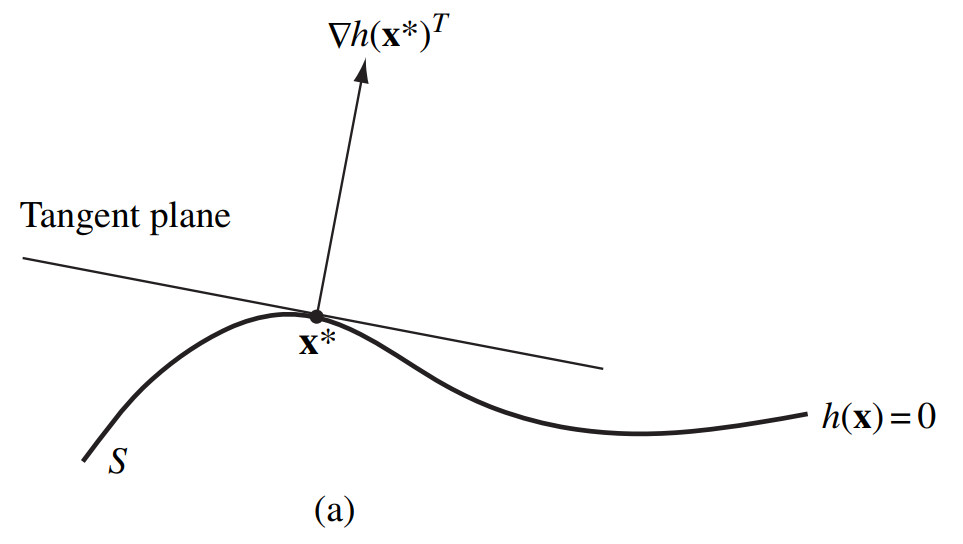
\includegraphics[scale=0.4]{\pref/tan-1dim.png}
\centering
    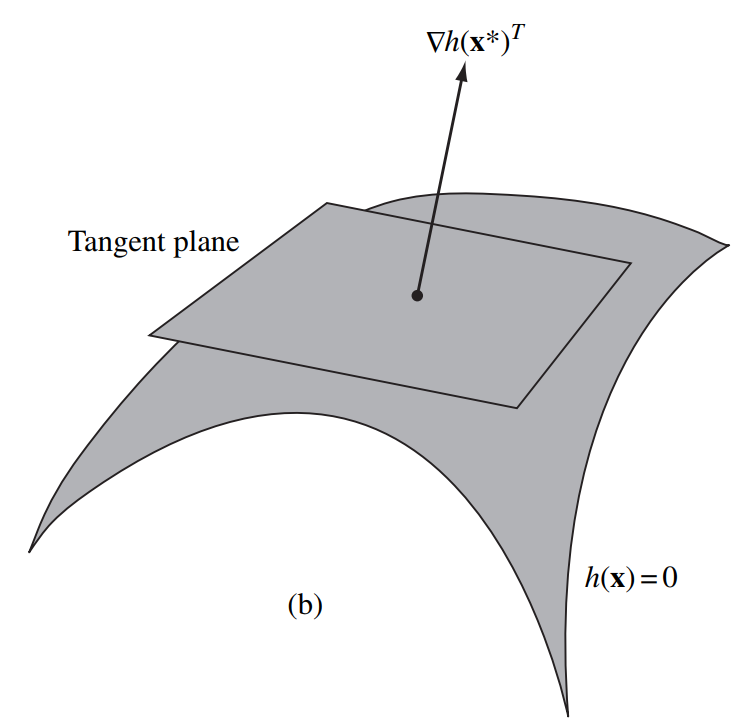
\includegraphics[scale=0.4]{\pref/tan-2dim.png}
\caption{切空间的示意图.}
\label{fig:tangent-space}
\end{figure}
    
我们把刚刚得到的垂直于$\nabla {h(x^\ast)y}$的子空间(即正交补空间)记作
    \[M=\{{y}\in\R^n:\nabla {h(x^\ast)y}=0\}.\]
我们已经证明$T_{x^\ast}(S)\subseteq M$. 反过来,在什么条件下会有$M=T_{x^\ast}(S)$?为此,我们引入\emph{正规点}的概念. 

\begin{definition}[正规点]\label{def:regular-point}\index{正规点}
考虑优化问题 \eqref{eq:eq-constraint-only-differentiable},当一个点${x^\ast}\in\Omega$满足约束${h(x^\ast)}=0$,且梯度向量$\nabla h_1({x^\ast}),\nabla h_2({x^\ast}),\dots,\nabla h_m({x^\ast})$线性无关时,它被称作该约束的\textbf{正规点}. 
\end{definition}

直观上来说,正规点上每一条约束都起到了实际的作用,因此梯度向量$\nabla h_i({x^\ast})$形成了一个线性无关的集合,张成了空间$M^\perp$. 此时,切空间恰好完全垂直于$M^\perp$,即$T_{x^\ast}(S)=M$. 这一几何直观见\Cref{fig:tan-2constraint},点${x^\ast }$处的两个等式约束共同确定了该点的切空间. 因此,在正规点,用约束函数的梯度来描述切空间是可行的. 
    \begin{figure}
        \centering
        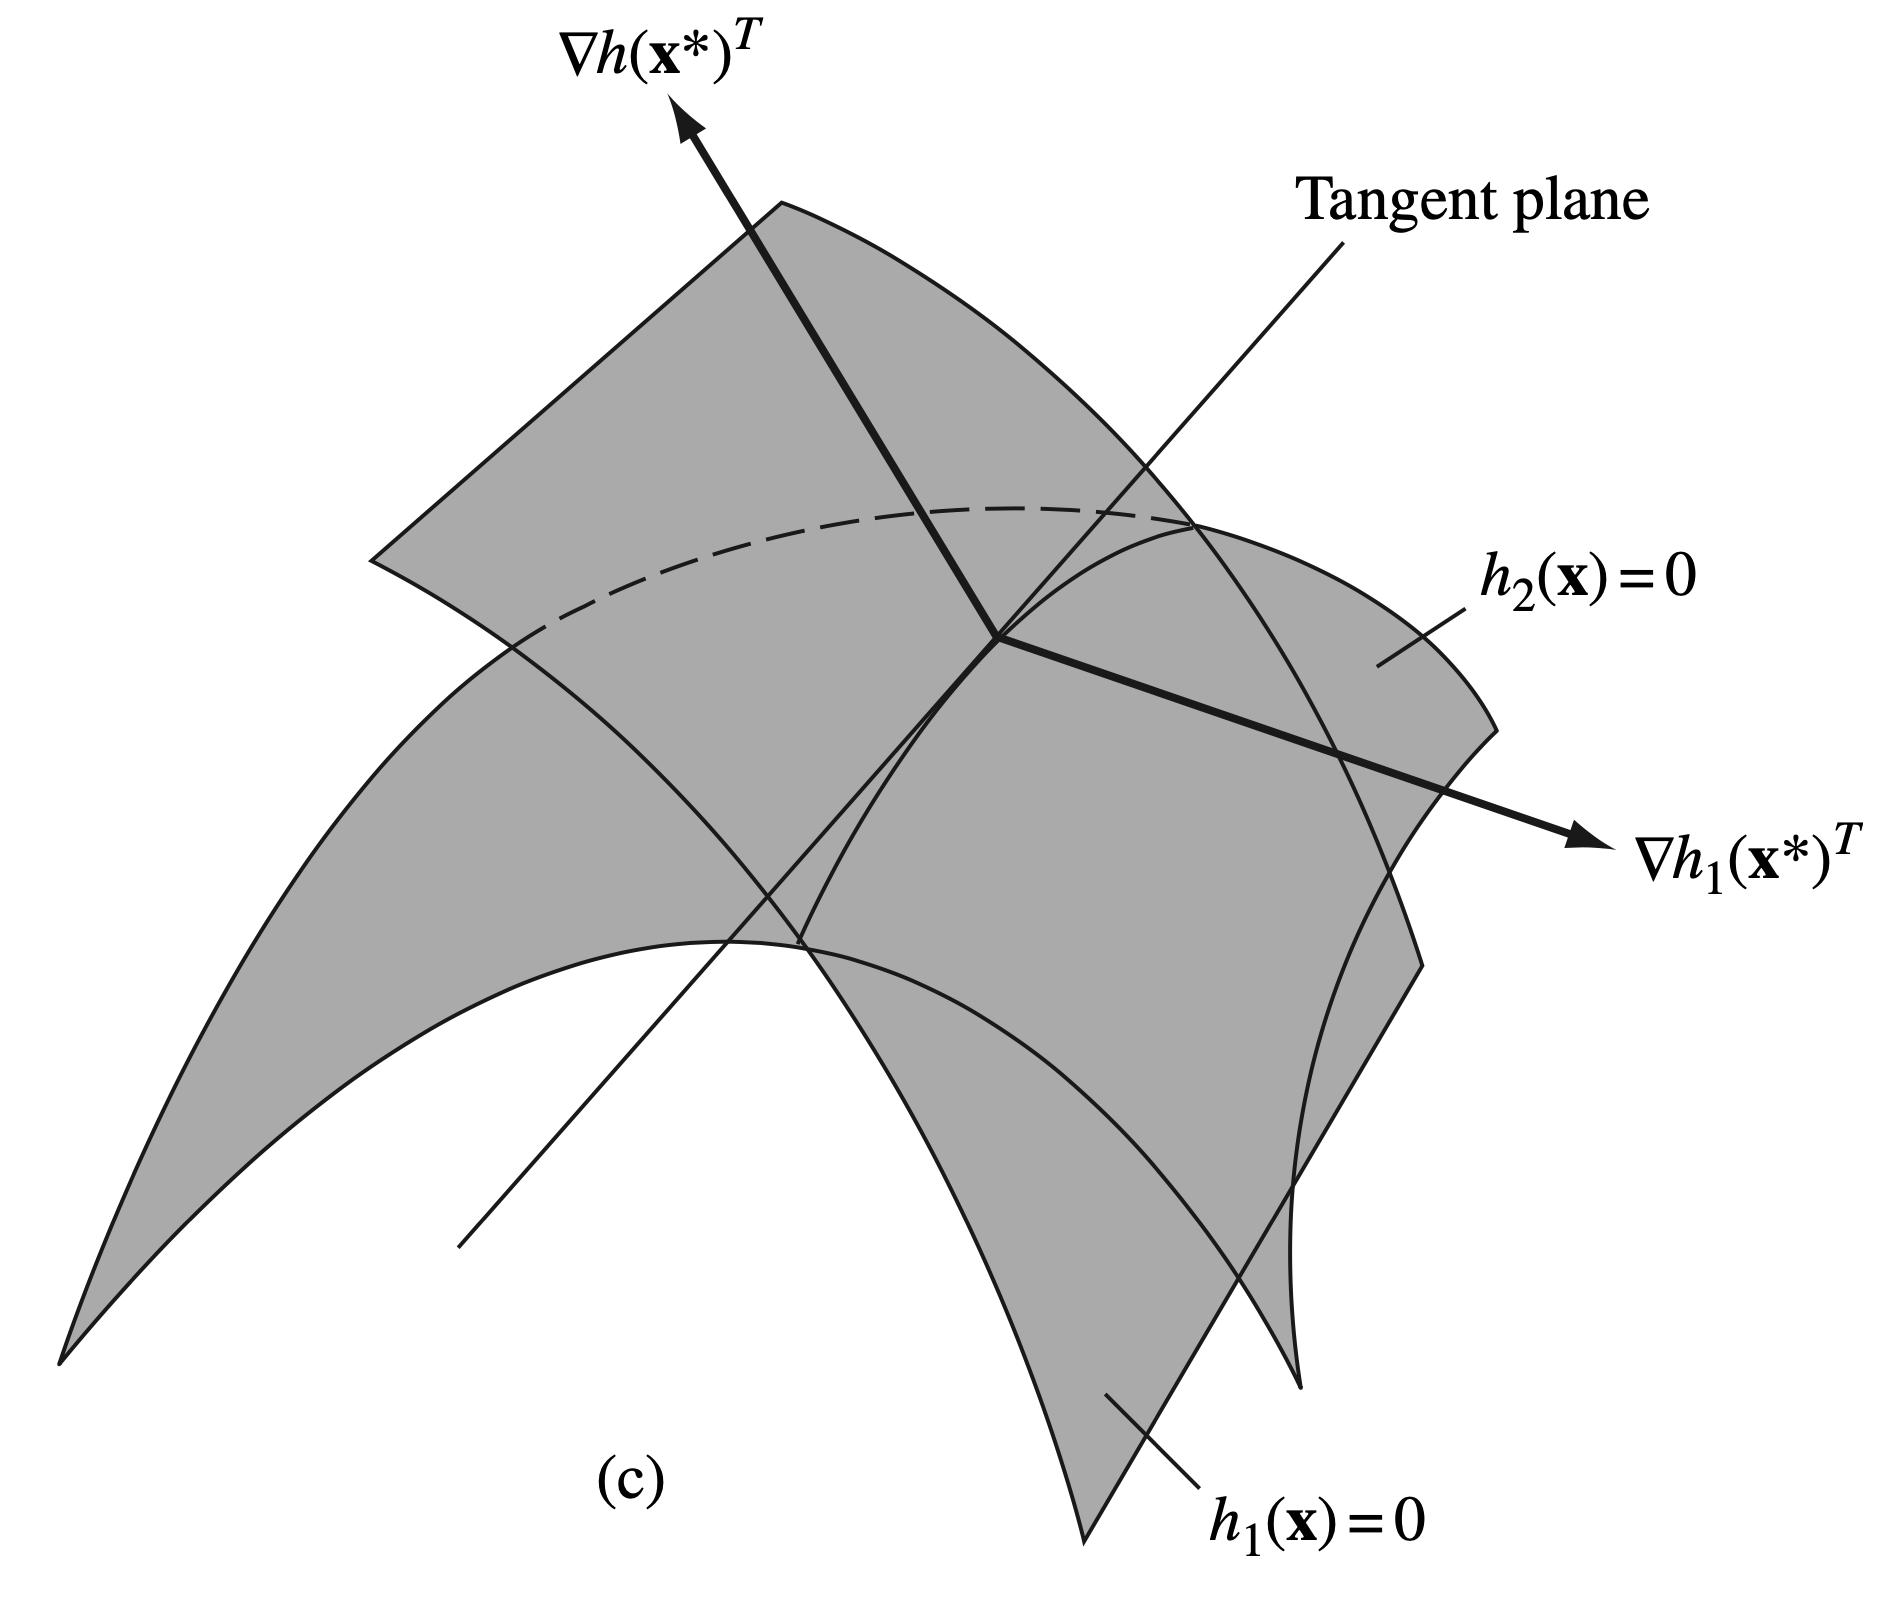
\includegraphics[scale=0.17]{\pref/tan-2constraint.png}
        \caption{正规点示意图. }
        \label{fig:tan-2constraint}
    \end{figure}

\begin{theorem}[正规点切空间刻画定理]
设曲面$S\subseteq\R^n$由约束$h(x)=0$定义,${x^\ast}\in S$是正规点,那么,
\[T_{x^\ast}(S)=M=\{{y:\nabla h(x^\ast)y=0}\}.\]
\end{theorem}
该定理的证明需要隐函数定理,对微积分要求较高,我们这里略去.

有了切空间的准备,现在我们要对正规点推导带约束的优化问题的极值条件. 考虑优化\eqref{eq:eq-constraint-only-differentiable},设$x^\ast$ 是一个约束${h(x)=0}$一个正规点,同时也是函数$f$的一个在可行域中的极值点.

\begin{lemma}\label{lemma:eq-opt-cond-1}
对$y\in\R^n$,如果$\nabla {h(x^\ast)y=0}$,那么$\nabla f({x^\ast}){y}=0$.
\end{lemma}

\begin{proof}
因为$x^\ast$是正规点,根据正规点切空间刻画定理,$\nabla h(x^*)y=0$等价于$y$是${x^\ast}$处的切空间中的向量. 根据定义,存在该约束曲面内的某个光滑曲线${x}(t)$,经过点${x^\ast}$,并且以$y$为切向量. 那么,${x}(0)={x^\ast}$,${\dot{x}}(0)={y}$,且${h(x(t))=0}$在区间$-a\le t\le a$上成立(对某个正数$a$). 因为点${x^\ast}$是一个函数$f$的受等式约束的极值点,我们有
\[\left.\frac{\d}{\d t}f({x}(t))\right|_{t=0}=0\iff \nabla f({x^\ast})y=0.\]
\end{proof}

\Cref{lemma:eq-opt-cond-1} 对任意$y\in\R^n$都成立,根据线性代数零空间的性质,这等价于$\nabla f(x^*)$是$\nabla h_i(x^*)$的线性组合,即
\[\nabla f(x^*)=\sum_i\lambda_i\nabla h_i(x^*).\]
据此,我们得到条件极值的一阶必要条件:
\begin{theorem}[条件极值的一阶必要条件]\label{thm:eq-opt-cond-1}\index{一阶必要条件}
    令${x^\ast}$是一个$f$的满足约束${h(x)=0}$的正规极值点. 那么存在一个${\lambda}\in \R^m$使得$$\nabla f({x^\ast})+{\lambda^\t \nabla h(x^\ast)=0}. $$
\end{theorem}

一阶必要条件$\nabla f({x^\ast})+{\lambda^\t}\nabla {h(x^\ast)=0}$以及约束${h(x^\ast)=0}$给出了$n+m$个等式,包含${x^\ast,\lambda}$在内的$n+m$个变量. 因此在非退化的情况下,他们给出了一个唯一解. 

引入与这个约束问题对应的Lagrange函数:
        $$l({x,\lambda})=f({x})+{\lambda^\t h(x)}.$$
$\lambda$被称为\emph{Lagrange乘子}\index{Lagrange乘子}. 必要条件可以被写作:
\begin{align*}
    \nabla_x l({x,\lambda})&=0,\\
    \nabla_{\lambda} l({x,\lambda})&=0.
\end{align*}


\begin{example}[最大熵]\label{ex:max-entropy}
考虑一个离散的概率分布,其分布列为$p_i=\Pr(X=x_i),i=1,\dots,n$. 该分布的熵为
$$\epsilon = -\sum_{i=1}^n p_i \log p_i.$$
该分布的均值为$\sum_{i=1}^n x_i p_i$. 

如果均值固定为$m$,求解使熵最大化的参数可以被转化成以下问题:
\begin{align*}
\max\quad&-\sum_{i=1}^n p_i\log p_i \\
\text{s.t.}\quad& \sum_{i=1}^n p_i=1, \\
&\sum_{i=1}^n x_i p_i=m, \\
&p_i\ge 0, \qquad i=1,2,\dots,n.
\end{align*}

我们先忽略非负约束,假设这些约束不会被触发. 引入两个Lagrange乘子,$\lambda$和$\mu$,则Lagrange函数为
$$l=\sum_{i=1}^n (-p_i\log p_i+\lambda p_i+\mu x_ip_i)-\lambda-\mu m.$$
由一阶必要条件,$-\log p_i -1+\lambda+\mu x_i=0$,$i=1,2,\dots,n$. 因此,
$$p_i=\exp((\lambda-1)+\mu x_i),\quad i=1,2,\dots, n.$$
注意$p_i>0$,所以非负约束确实没有被触发. Lagrange乘子$\lambda$和$\mu$是两个用来保证等式约束被满足的参数. 
\end{example}

\section{Karush–Kuhn–Tucker条件}
现在加入不等式约束,考虑以下形式的问题:
\begin{equation}
\begin{aligned}
\min\quad& f({x}) \\
\text{s.t.}\quad& {h(x)=0}, \\
&{g(x)\le0}. 
\end{aligned}\label{eq:ineq-constraint-inequality-differentiable}
\end{equation}
假设$f$和${h}$和前面一样,${g}$是一个$p$维的函数,$f,{h,g}\in C^1$. 

我们推广正规点$x^\ast$的定义为:
\begin{definition}[正规点]\index{正规点}
考虑优化问题 \eqref{eq:ineq-constraint-inequality-differentiable},点$x^\ast$被称为\textbf{正规点},如果
\begin{itemize}
    \item 它满足约束:$h(x^\ast)=0, g(x^\ast)\le 0$.
    \item 令$J$为满足$g_j({x^\ast})=0$的下标$j$的集合(激活的约束). 那么,梯度向量$\nabla h_i({x^\ast})$,$\nabla g_j({x^\ast})$,$1\le i \le m$,$j\in J$是线性无关的.
\end{itemize}
\end{definition}

换言之,此时的正规点不仅考虑等式约束,还要考虑起作用的或者说被激活的不等式约束,这些不等式约束相当于等式约束. 类似Lagrange乘子法,此时的一阶必要条件为:

\begin{theorem}[Karush-Kuhn-Tucker条件]\label{thm:KKT}\index{Karush-Kuhn-Tucker条件}\index{一阶必要条件}
令${x^\ast}$为优化问题 \eqref{eq:ineq-constraint-inequality-differentiable} 的正规极小值点,那么,存在向量${\lambda}\in\R^m$和向量${\mu}\in \R^p$且${\mu\ge 0}$使得
\begin{align}
    \nabla f({x^\ast})+\lambda^\t \nabla {h(x^\ast)}+{\mu}^\t \nabla {g(x^\ast)}&={0},\label{eq:KKT-1}\\
    {\mu^\t g(x^\ast)}&=0.\label{eq:KKT-2}
\end{align}
\end{theorem}

\begin{proof}
首先,因为${\mu\ge 0}$且${g(x^\ast)\le 0}$,\eqref{eq:KKT-2} 等价于:${\mu}$的一个分量非零仅当对应的约束被激活(即取到等号). 这是一个互补松弛条件,即${g(x^\ast)}_i<0$可得出$\mu_i=0$,以及$\mu_i>0$可得出${g(x^\ast)}_i=0.$

设被激活的下标为$J$. 因为${x^\ast}$是约束集合上的一个极小点,它也是满足等式约束$h(x)=0,g_i(x)=0,i\in J$的极小点. 因此,在新的等式约束问题中,${x^\ast}$的邻域中存在Lagrange乘子,满足一阶必要条件. 我们得出结论:一阶必要条件 \eqref{eq:KKT-1} 成立,且若$g_j({x^\ast})\neq0$,则$\mu_j=0$.(于是也有 \eqref{eq:KKT-2} 成立)

现在还需要证明${\mu \ge 0}$. 用反证法,假设$\mu_k<0$对某个$k\in J$成立. 设$S$为其他所有被激活的约束在${x^\ast}$处定义的曲面,$M=T_{x^\ast}(S)$. 因为$x^\ast$是正规的,存在${y}\in M$且$\nabla g_k({x^\ast})y<0$. 令${x}(t)$为一条在$S$内且经过${x^\ast}$(此处$t=0$)的曲线,且有$\dot{{x}}(0)={y}$. 则对于充分小的$t\ge 0$,${x}(t)$是可行的,由 \eqref{eq:KKT-1} 以及$y\in M$,
\begin{align*}
    \left.\frac{\d f({x}(t))}{\d t}\right|_{t=0}=&\nabla f({x^\ast})y\\
    =&-\lambda^\t \nabla {h(x^\ast)}y-{\mu}^\t \nabla {g(x^\ast)}y\\
    =&-\mu_k\nabla g_k({x^\ast})y<0. 
\end{align*}
这与${x^\ast}$是极小点矛盾. 
\end{proof}

\begin{remark}
这一证明具有很强的几何直观,关键在于找一个可行的方向使得函数值下降. 非常需要注意的是,这一证明并不能用于否证$\mu_k>0$. 此时需要取${y}\in M$使得$\nabla g_k({x^\ast})y>0$. 然而此时对应的$x(t)$不再可行,因为对充分小的$t>0$,$g_k(x(t))>0$,违背了约束的条件.
\end{remark}

下面我们来看一个运用KKT条件的例子:
\begin{example}
考虑问题
\begin{align*}
    \min \quad &2x_1^2+2x_1x_2+x_2^2-10x_1-10x_2 \\
    \text{s.t.}\quad &x_1^2+x_2^2\le 5, \\
    & 3x_1+x_2\le 6.
\end{align*}
KKT条件为(注意,一阶必要条件还需要加入问题中的约束条件)
\begin{align*}
    4x_1+2x_2-10+2\mu_1x_1+3\mu_2&=0, \\
    2x_1+2x_2-10+2\mu_1x_2+\mu_2&=0, \\
    \mu_1(x_1^2+x_2^2-5)&=0, \\
    \mu_2(3x_1+x_2-6)&=0,\\
    \mu_i&\ge 0,\quad i=1,2.
\end{align*}
为了求解此类问题,我们假设一些约束被激活,然后检查所得出的Lagrange乘子的符号正负. 在这个问题中,我们可以尝试假设有0,1,2个约束被激活. 

假设第一个约束被激活,第二个约束没有被激活,得出等式
\begin{align*}
4x_1+2x_2-10+2\mu_1x_1&=0, \\
2x_1+2x_2-10+2\mu_1x_2&=0, \\
x_1^2+x_2^2&=5.
\end{align*}
可得解$x_1=1,x_2=2,\mu_1=1.$

由于$3x_1+x_2=5$,因此第二个约束也被满足了. 因此,因为$\mu_1 > 0$,我们得出结论,这个解满足一阶必要条件. 
\end{example}

\section{Lagrange对偶}
\subsection{Lagrange定理}
现在,我们不再假设函数可微,我们考虑极值点的零阶必要条件\index{零阶必要条件},首先考虑只有等式约束的情形:
    \begin{equation}
          \begin{aligned}
        \min&\quad f({x}) \\
        \text{s.t.}\quad& {h(x)=0}, \\
        &{x}\in\Omega.
        \end{aligned}\label{eq:eq-zero-cond}
    \end{equation}
如果函数$f$是凸函数,$m$维函数${h}$是仿射的,并且集合$\Omega\subset \R^n$是是凸的,那么这个规划问题是一个\emph{凸规划问题}\index{凸规划问题}. 

为了给这样的问题一个一阶必要条件,我们依然需要引入正规性条件. 此时正规性不再仅仅只对一个点,而是对仿射函数$h$.

\begin{definition}[正规性条件]\index{正规性条件}
一个仿射函数${h}$关于集合$\Omega$是\textbf{正规的},指的是像集$h(\Omega)=\{y:\exists x\in\Omega\ h(x)=y\}$包含${0}$处的一个开球邻域. 也就是说,$h(\Omega)$包含一个形如$\{y:\norm{y}<\epsilon\}$(对某个$\epsilon>0$)的集合. 
\end{definition}

\begin{remark}
这个条件是一阶正规点定义的推广. 如果${h}$在点${x^\ast}$有连续的导数,那么一阶正规性条件意味着$\nabla{h(x^\ast)}$是满秩的,并且由隐函数定理可知存在一个$\epsilon>0$使得对于任意满足${\norm{y-h(x^\ast)}}<\epsilon$的${y}$,都有一个${x}$使得${h(x)=y}$. 换言之,存在一个${y^\ast=h(x^\ast)}$周围的开球.
\end{remark}

我们可以用Lagrange乘子来表述零阶必要条件:
\begin{theorem}[零阶必要条件,等式约束情形]\label{thm:eq-zero-cond}\index{零阶必要条件}
假设$\Omega\subset\R^n$是凸的,$f$是$\Omega$上的凸函数,${h}$是一个$\Omega$上的$m$维仿射函数. 假设${h}$是对于$\Omega$正规的. 如果${x^\ast}$是 \eqref{eq:eq-zero-cond} 的解,那么存在${\lambda}\in \R^m$使得${x^\ast}$是以下Lagrange问题的解:\begin{align*}
    \min\quad& f({x})+{\lambda^\t h(x)}\\
    \text{s.t.}\quad & x\in\Omega.
\end{align*}
\end{theorem}

这一定理证明的关键在于引入\emph{原始函数}. 对应于问题\eqref{eq:eq-zero-cond} 的\textbf{原始函数}\index{原始函数}是:$$\omega({y})=\inf\{f({x}):{h(x)=y,x}\in\Omega\},\quad y\in h(\Omega).$$


\begin{proof}[零阶必要条件的证明]
令$f^\ast=f({x^\ast})$. 定义$\R^m\times\R$内的集合$A$和$B$为:
\begin{align*}
    A&=\{(y,r):r\ge \omega({y}),{y}\in h(\Omega)\},\\ 
    B&=\{(y,r):r\le f^\ast,y=0\}.
\end{align*}
$A$是$\omega$的上图,$B$是$f^\ast$向下延申并与原点对齐的垂线. $A$和$B$都是凸集. 他们唯一的公共点是$(0,f^\ast)$. 由超平面分离定理可知,存在一个超平面分离$A$和$B$. 这个超平面可以被表示成一个在$\R^m\times\R$内的形如$(\lambda,s),\lambda\in \R^{m}$的非零向量,还有一个分离常数$c$. 分离条件是$$sr+{\lambda^\t y}\ge c,\quad\forall(y,r)\in A,\quad sr+{\lambda^\t y}\le c,\quad\forall(y,r)\in B.$$ 
这一过程的示意图见\Cref{fig:sep-hyperplane-eq}.

\begin{figure}[ht]
    \centering
    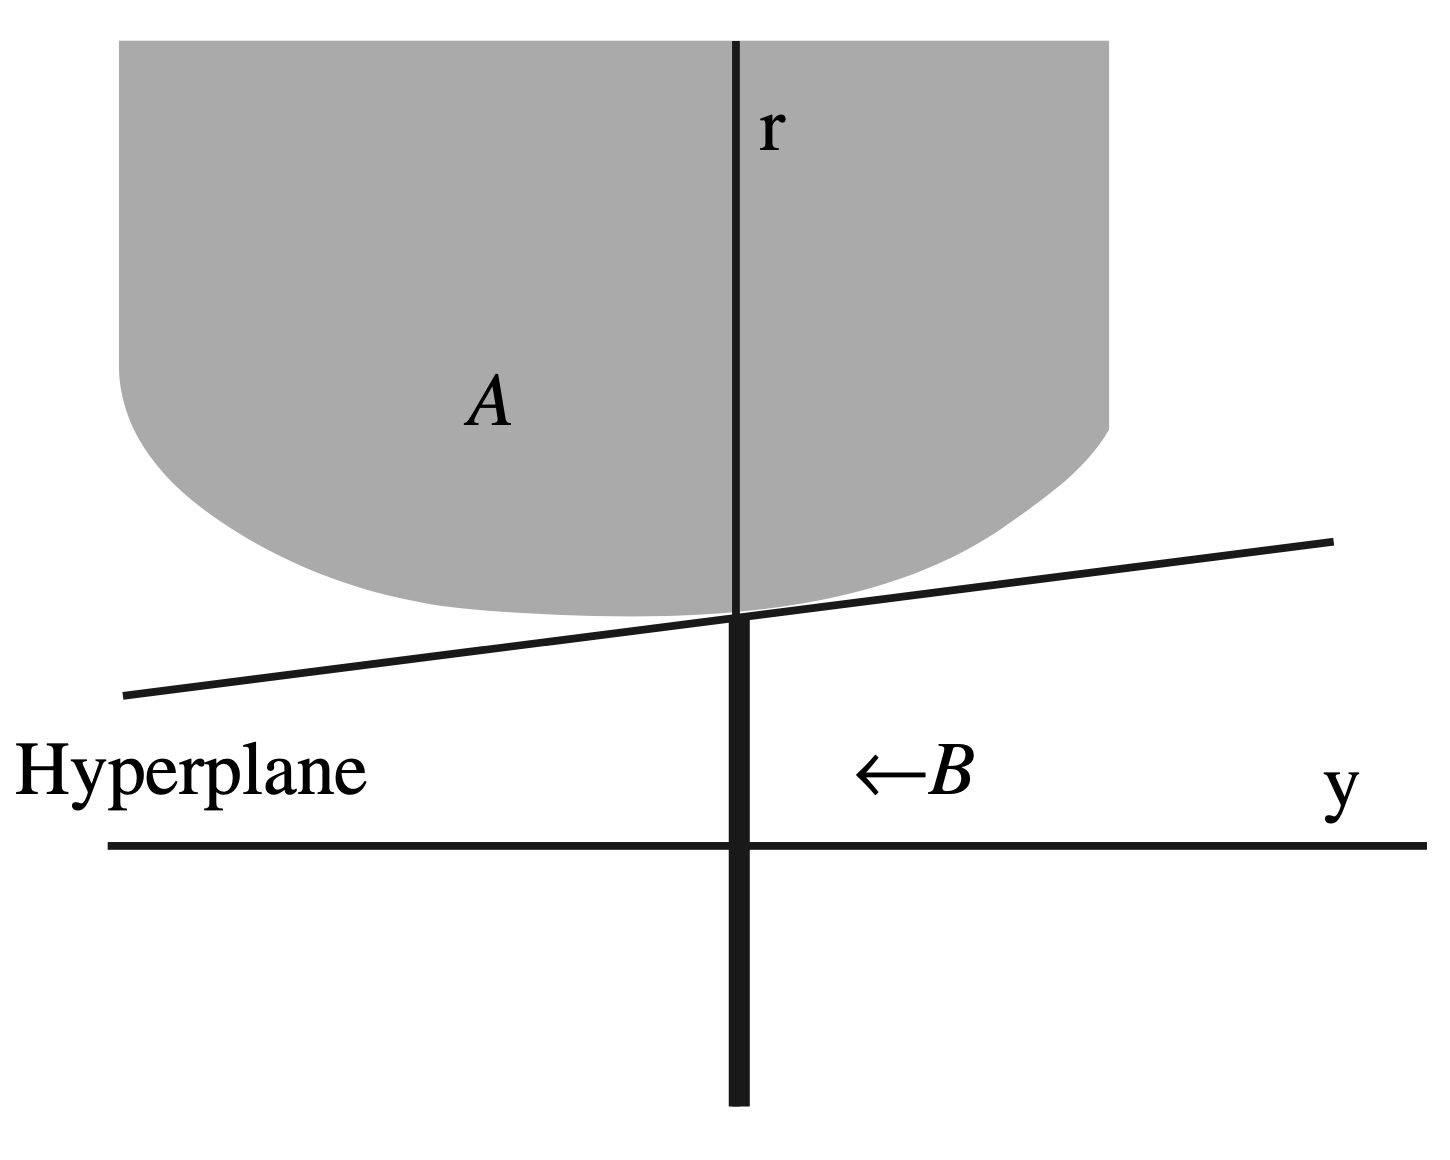
\includegraphics[scale=0.3]{\pref/sep-hyperplane-eq.png}
    \caption{证明示意图. }
    \label{fig:sep-hyperplane-eq}
\end{figure}

注意到$s\ge 0$,否则取$|r|$非常大的负数$r$,点$(r,{0})\in B$违反第二个分离不等式. 几何上看,若$s=0$,超平面将垂直. 我们来证明$s\neq 0$. 假设$s=0$,因为$s$和${\lambda}$不能都是$0$,${\lambda\neq 0}$. 因为分离超平面必须包含点$(f^\ast,{0})$,从第二个分离不等式得$c=0$. 由$h$的正规性,以${0\in h(\Omega)}$为中心的某个球包含在$h(\Omega)$中,任取$y$属于这个开球. 第一个分离不等式左侧为${\lambda^\t y}$,它对于某些${y}$来说是负的. 这违背第一个分离不等式. 因此$s\neq 0$,继而$s>0$. 

不失一般性,可以假设$s=1$. 假设$x\in\Omega$. 那么$(h(x),f(x))\in A$且$(0,f(x^\ast))\in B$. 因此,由分离不等式可知,我们有$$f({x})+{\lambda^\t h(x)}\ge f({x^\ast})=f({x^\ast})+{\lambda^\t h(x^\ast)}.$$ 因此${x^\ast}$是优化问题 \eqref{eq:eq-zero-cond} 解. 
\end{proof}

我们再考虑只有不等式约束的模型
\begin{equation}
    \begin{aligned}
    \min\quad & f({x})\\
    \text{s.t.}\quad& {g(x)\le 0},\\
    &{x}\in\Omega.
\end{aligned}\label{eq:ineq-zero-cond}
\end{equation}
其中,${g}$是一个$p$维的函数. 


然后我们引入正规性条件. 对于不等式约束来说,正规性条件也被称为做\emph{Slater条件}. 

\begin{definition}[Slater条件]\index{正规性条件}\index{Slater条件}
考虑优化问题 \eqref{eq:ineq-zero-cond},令
\[D=\{z\in \R^p:\exists x\in\Omega\ {g(x)\le z}\}.\]
正规性条件(Slater条件)为:存在一个$z^\prime\in D$使得$z^\prime<0$. 
\end{definition}
直观来说,Slater条件指的是存在满足约束的内点.

类似地,我们可以用Lagrange乘子来表述零阶必要条件:
\begin{theorem}[零阶必要条件,不等式情形]\label{thm:ineq-zero-cond}\index{零阶必要条件}
假设$\Omega$是一个$\R^n$的凸子集,且$f$和${g}$是凸函数. 假设优化问题 \eqref{eq:ineq-zero-cond} 满足正规性条件,${x^\ast}$是该问题的解,那么存在一个向量${\mu}\in \R^p$满足$\mu\ge 0$使得${x^\ast}$是下述Lagrange问题的解:
\begin{align*}
\min\quad &f({x^\ast})+\mu^\t g(x)\\
\text{s.t.}\quad& x\in\Omega.
\end{align*}
此外,${\mu^\t g(x^\ast)}=0.$
\end{theorem}

这一定理的证明类似于\Cref{thm:eq-zero-cond} 的证明. 首先还是引入原始函数. 问题 \eqref{eq:ineq-zero-cond} 对应的原始函数\index{原始函数}为:
    $$\omega({z})=\inf\{f({x}):g(x)\le{z},x\in\Omega\},z\in D.$$


\begin{proof}[证明概要]
令$f^\ast=f({x^\ast})$. 在$\R^{p}\times\R$内定义两个集合
\begin{align*}
    A&=\{(z,r):r\ge \omega(z), z\in D\},\\
    B&=\{(z,r):r\le f^\ast, z\leq 0\}.
\end{align*}
$A$和$B$都是凸的. 证明依然是构造$A,B$的分离超平面,正规性条件保证了超平面不会是垂直的. 这个过程的示意见图\Cref{fig:sep-hyperplane-ineq}.
\begin{figure}
    \centering
    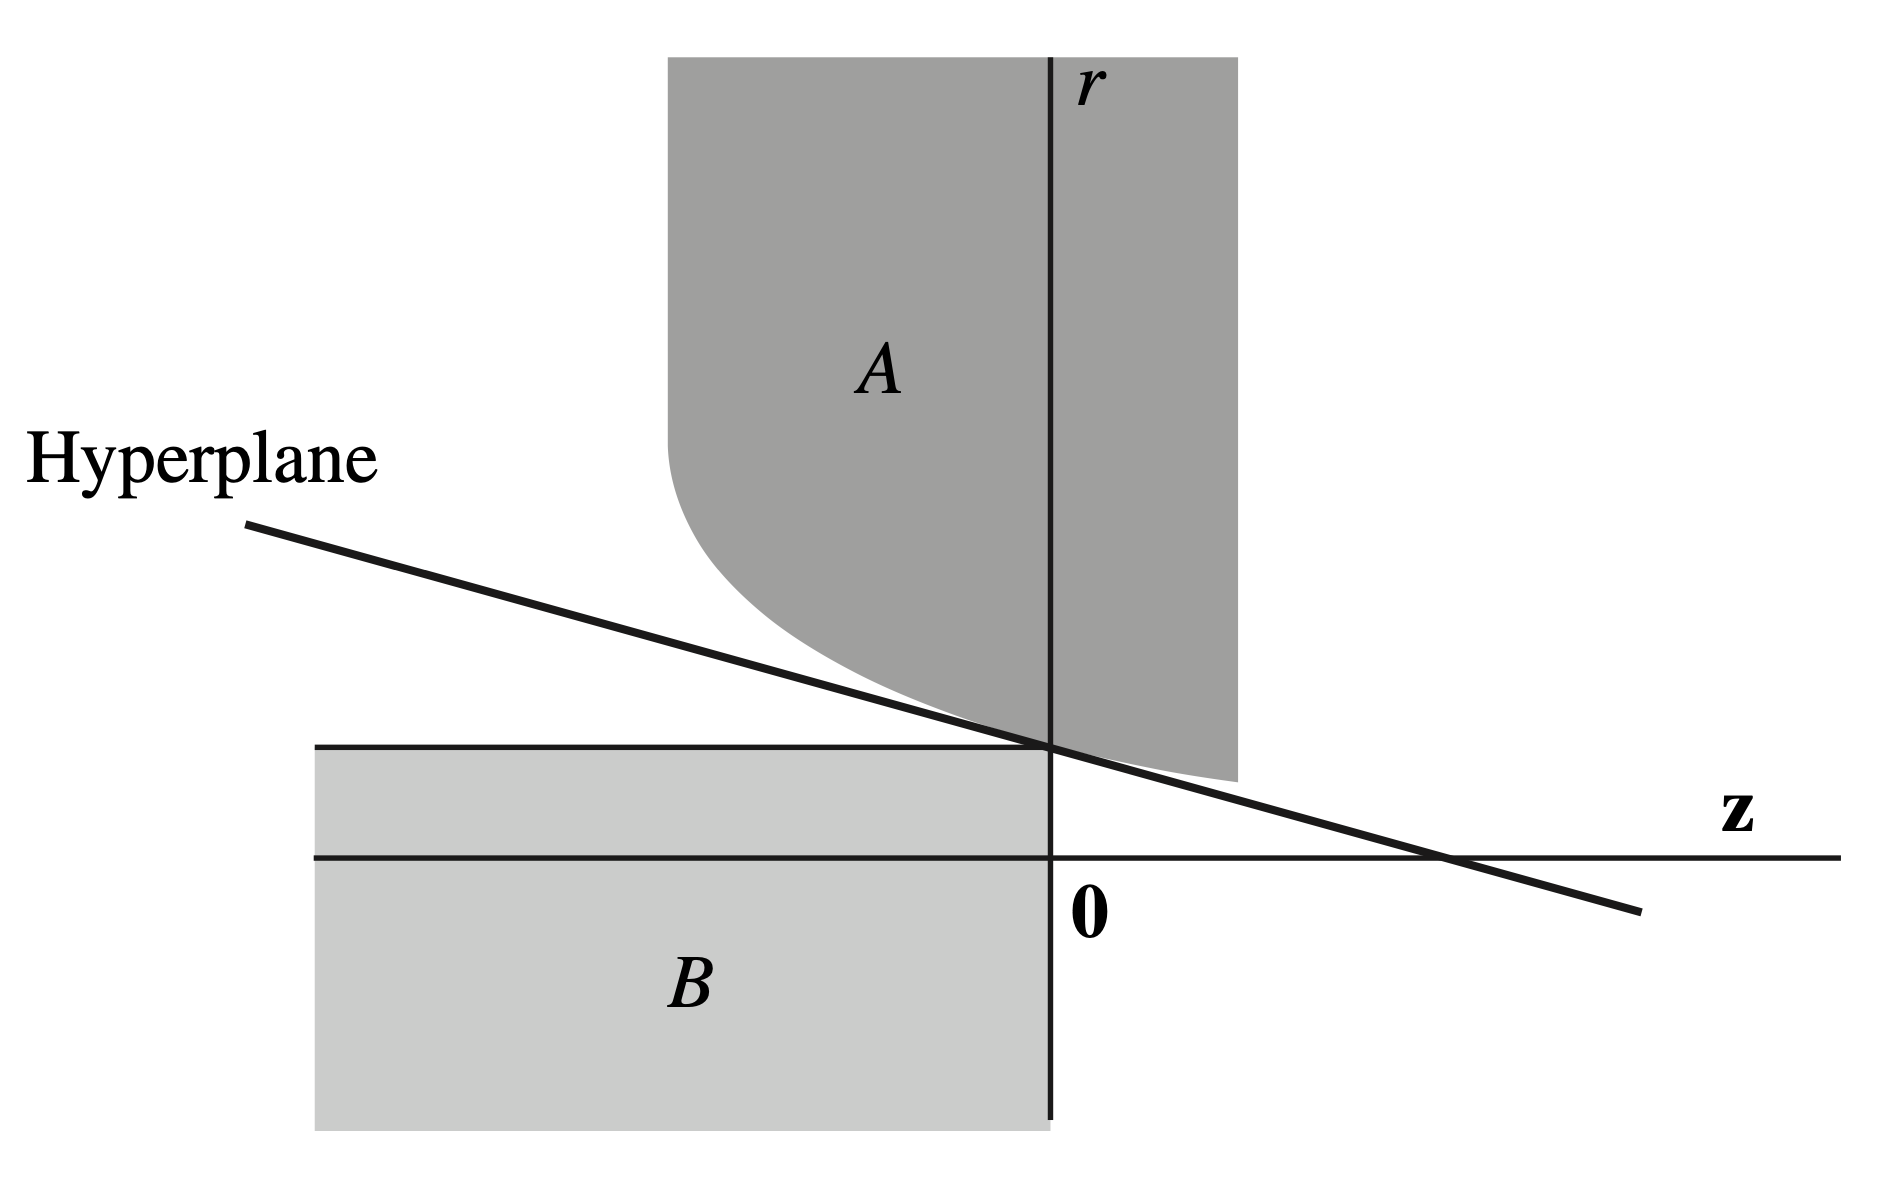
\includegraphics[scale=0.3]{\pref/sep-hyperplane-ineq.png}
    \caption{证明示意图. }
    \label{fig:sep-hyperplane-ineq}
\end{figure}

条件$\mu^\t g(x^\ast)=0$是互补松弛条件,这一讨论类似KKT条件. 
\end{proof}

现在,我们考虑一般情形,
    \begin{equation}
          \begin{aligned}
        \min\quad & f({x}) \\
        \text{s.t.}\quad& {h(x)=0}, \\
        &g(x)\leq 0, \\
        &{x}\in\Omega.
        \end{aligned}\label{eq:mix-zero-cond}
    \end{equation}
组合以上两个零阶必要条件,我们得到一般情形的Lagrange定理.

\begin{theorem}[Lagrange,零阶必要条件,混合情形]\label{thm:mix-zero-cond}\index{零阶必要条件}\index{Lagrange定理}
假设$\Omega\subset \R^n$是凸集. $f$和${g}$是一维和$p$维的凸函数,${h}$是维数为$m$的仿射函数. 假设${h}$满足对于$\Omega$的正规性条件,且$g$在 \eqref{eq:mix-zero-cond} 的可行域上满足正规性条件. 假设${x^\ast}$是问题 \eqref{eq:mix-zero-cond} 的解. 那么存在向量${\lambda}\in \R^m$和${\mu}\in \R^p$满足${\mu}\ge {0}$使得${x^\ast}$是以下Lagrange问题的解:
\begin{align*}
\min\quad &f({x})+\lambda^\t h(x)+\mu^\t g(x) \\
\text{s.t.}\quad& x\in\Omega.
\end{align*}
此外,${\mu^\t g(x^\ast)}=0.$
\end{theorem}

\lhysays{举个例子}


\subsection{弱对偶定理,强对偶定理}
Lagrange定理有非常强的几何直观,这一直观最终导致了优化中的\emph{对偶理论}\index{对偶理论}. 先考虑不等式约束的情形:
\begin{equation}
    \begin{aligned}
    \min\quad & f({x})\\
    \text{s.t.}\quad& {g(x)\le 0},\\
    &{x}\in\Omega.
\end{aligned}\label{eq:ineq-dual}
\end{equation}
$\Omega\subset \R^n$是凸集,函数$f$和${g}$定义在$\Omega$上. 函数${g}$是$p$维的. 

回忆原始函数的定义:
        $$\omega({z})=\inf \{f({x}):g(x)\le z,x\in\Omega\}.$$

设$x^\ast$是 \eqref{eq:ineq-dual} 的解,$f^\ast=f(x^\ast)$,那么函数$\omega(z)$与纵轴的交点是$f^*$. 如果 \eqref{eq:ineq-dual} 没有解,那么$f^*=\inf\{f(x):g(x)\leq 0,x\in\Omega\}$就是纵轴与$\omega(z)$的交点. 考虑在$\omega(z)$以下的超平面,关注其纵截距(见图\Cref{fig:hyperplane-below}),我们用它产生对偶原理.
\begin{figure}
    \centering
    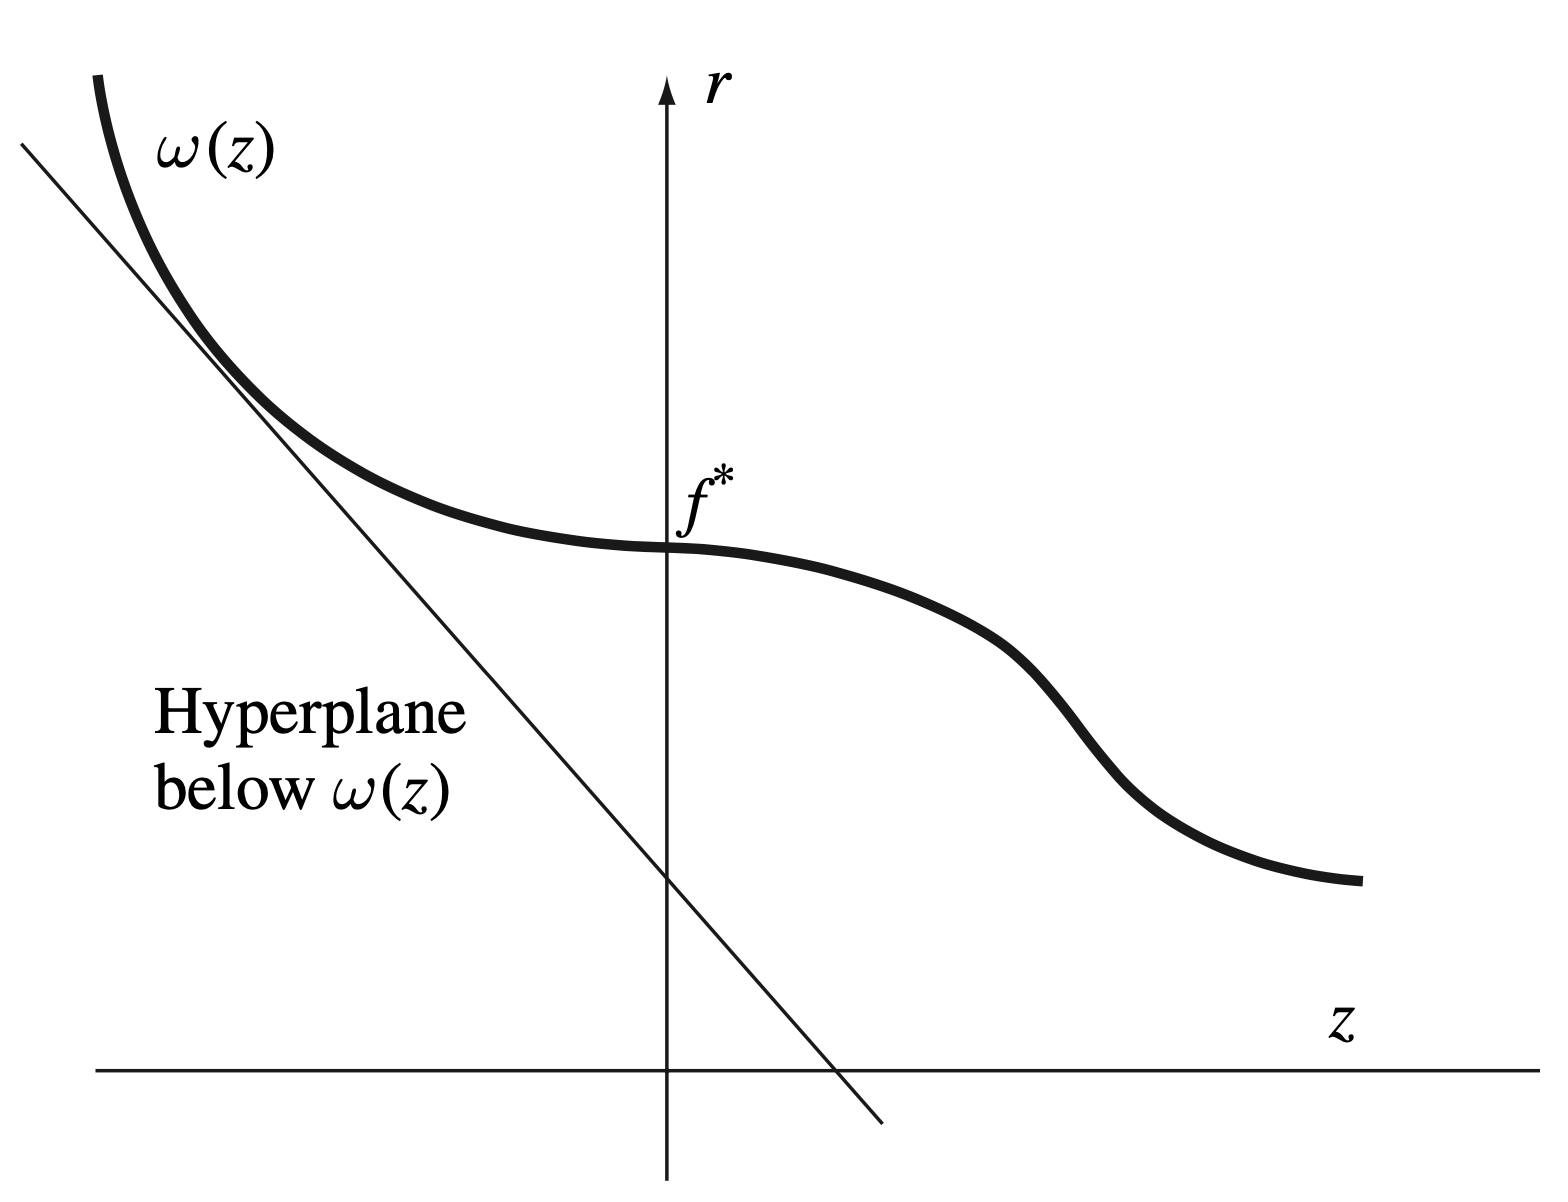
\includegraphics[scale=0.2]{\pref/hyperplane-below.png}
    \caption{纵截距的示意图.}
    \label{fig:hyperplane-below}
\end{figure}

为了刻画超平面以及其纵截距,我们引入对偶函数. 在$\R^p_{\geq 0}$上定义\textbf{对偶函数}\index{对偶函数}为:
$$\varphi({\mu})=\inf \{f({x})+{\mu^\t g(x)}:{x}\in\Omega\}.$$
定义其最大值为
    \[\varphi^*=\sup\{\varphi(\mu),\mu\geq 0\}.\]

我们很容易可以证明以下定理:

\begin{theorem}[弱对偶定理]\label{thm:weak-dual}\index{弱对偶定理}
    $\varphi^\ast\le f^\ast$.
\end{theorem}

\begin{proof}
    对任意${\mu \ge 0}$我们有
    \begin{align*}
        \varphi({\mu}) &=\inf\{f({x})+{\mu^\t g(x):x}\in\Omega\} \\
        & \le \inf\{f({x})+{\mu^\t g(x):g(x)\le 0,x}\in\Omega\} \\
        & \le \inf\{f({x}):{g(x)\le 0, x}\in\Omega\}=f^\ast.
    \end{align*}
    由此,$\varphi^\ast\le f^\ast$. 
\end{proof}

弱对偶定理也有非常几何的解释. 考虑向量$(\mu,1)\in \R^{p}\times\R$,${\mu}\ge{0}$和一个常数$c$. 关于$(z,r)$的方程$({\mu},1)^\t (z,r)=r+{\mu^\t z}=c$定义了一个$\R^{p}\times\R$内的超平面. 不同的$c$得到不同的超平面,他们都是平行的. 对于给定的$({\mu},1)$(即平行的超平面),选取一个最低的超平面,使得它刚刚碰到了原始函数上图边界. 假设${x_1}$是这个触点,有$r=f(x_1)$和$z=g(x_1)$. 那么$c=f({x_1})+{\mu^\t g(x_1)}=\varphi({\mu})$. 注意到此时$c=\varphi({\mu})$就是截距,这就是$\varphi(\mu)$的几何含义.

另一方面,求截距$c$(对偶函数值)的最大值$\varphi^*$,就是求位于原始函数之下的超平面的最大截距. 因此至少有$\varphi^*\leq f^*$,差$f^*-\varphi^*$被称为\emph{对偶间距}\index{对偶间距}. 这就是弱对偶定理,图示参见\Cref{fig:highest-hyperplane}.

\begin{figure}
    \centering
    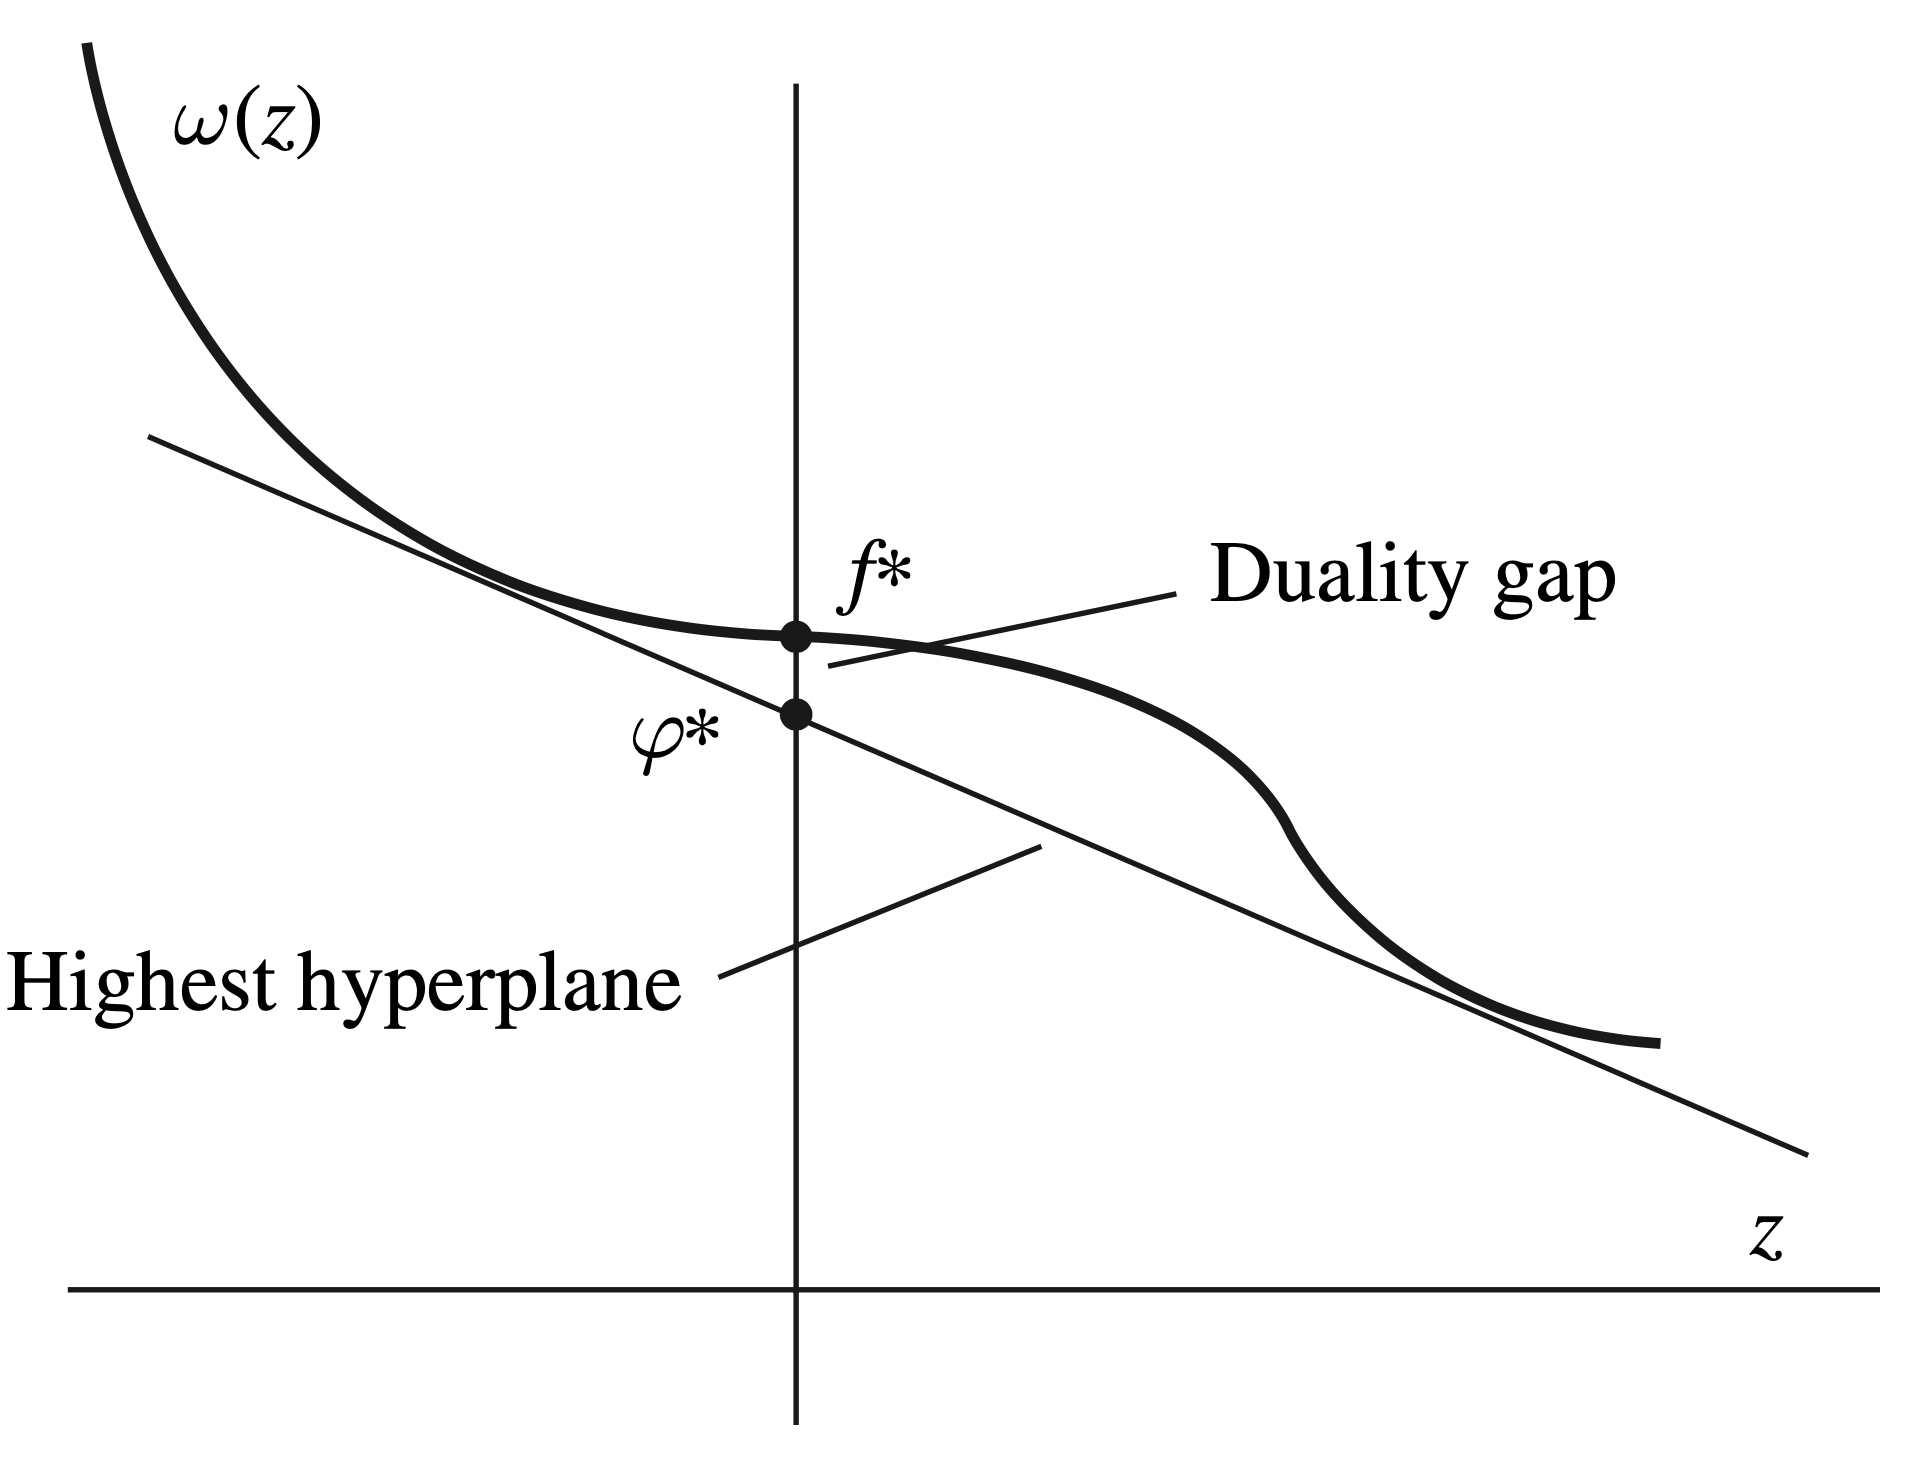
\includegraphics[scale=0.3]{\pref/highest-hyperplane.png}
    \caption{对偶间距的示意图.}
    \label{fig:highest-hyperplane}
\end{figure}

由此可以得到对偶性原理:位于$\omega$之下的超平面的最大截距等于刚刚碰到$\omega$的超平面的最小截距.

如果原始函数$\omega$是凸的,那么弱对偶定理可以被加强到强对偶定理,此时$\varphi^*$和$f^\ast$之间不再存在对偶间距,\Cref{fig:highest-hyperplane} 变成了\Cref{fig:strong-dual}.

\begin{figure}
    \centering
    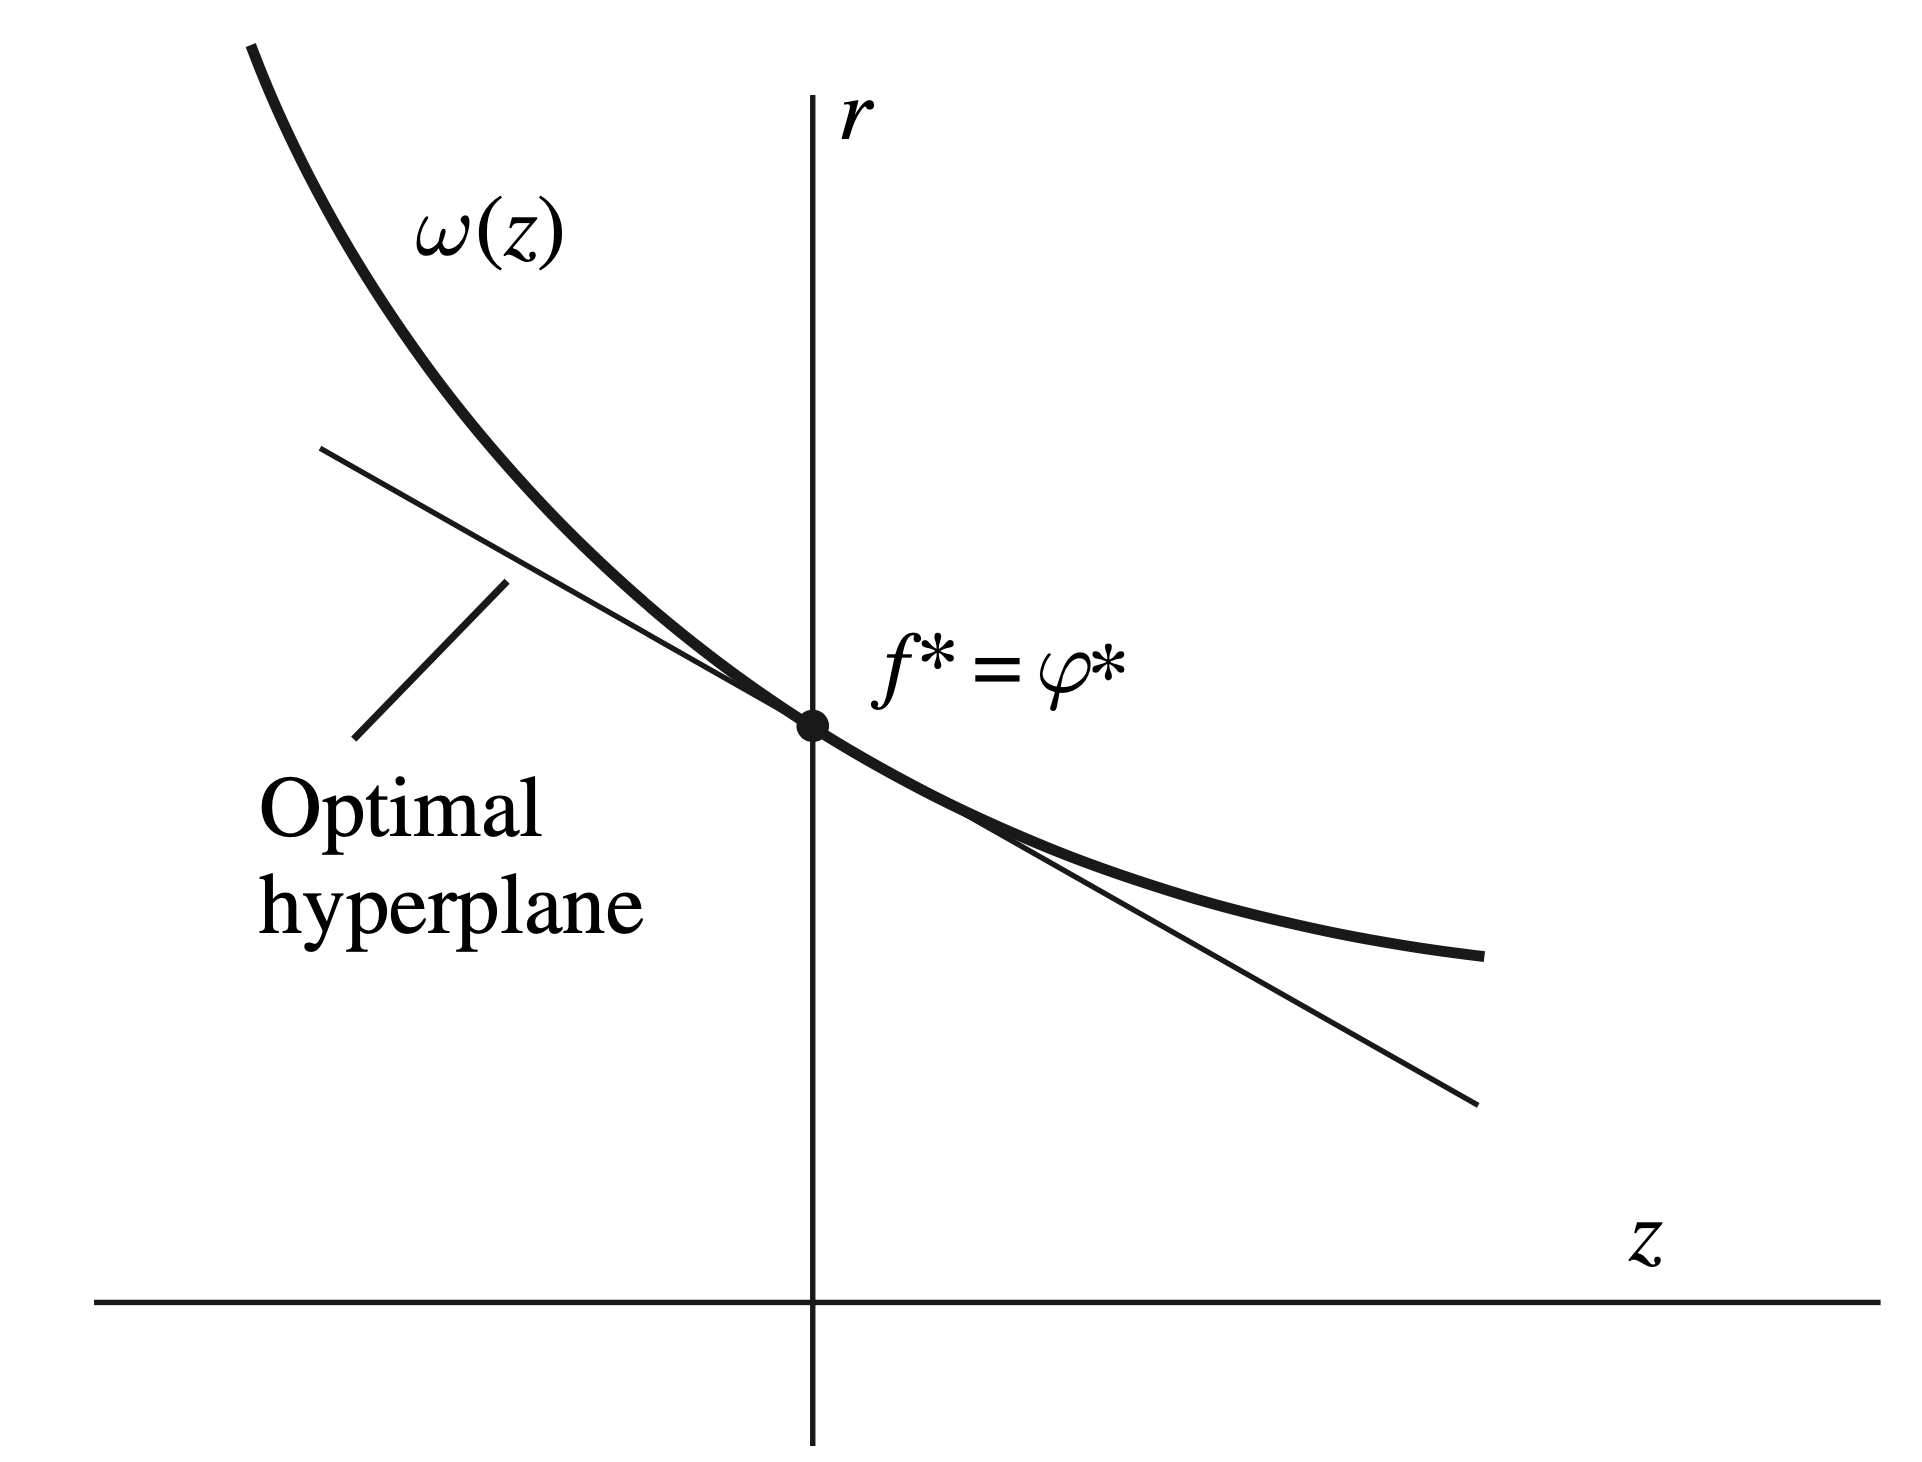
\includegraphics[scale=0.3]{\pref/strong-dual.png}
    \caption{强对偶定理的示意图.}
    \label{fig:strong-dual}
\end{figure}

下面我们叙述并证明强对偶定理. 我们直接考虑一般的优化问题.
\begin{equation}
        \begin{aligned}
    \min\quad & f({x}) \\
    \text{s.t.}\quad& {h(x)=0}, \\
    &g(x)\leq 0, \\
    &{x}\in\Omega.
    \end{aligned}\label{eq:mix-dual}
\end{equation}
其中,${h}$是$m$维仿射函数,${g}$是$p$维凸函数,$\Omega\subseteq\R^n$是凸集. 

原始函数\index{原始函数}可以写作
    \[\omega(y,z)=\inf\{f(x):\exists x\in\Omega\ h(x)=y, g(x)\leq z\}.\]
对偶函数\index{对偶函数}定义为:$$\varphi({\lambda,\mu})=\inf\{f({x})+{\lambda^\t h(x)+\mu^\t g(x):x}\in\Omega\}.$$
它的最大值记为
    $$\varphi^\ast=\sup\{\varphi({\lambda,\mu}):{\lambda}\in \R^m,{\mu}\in \R^p,{\mu}\ge {0}\}.$$

利用以上定义,我们可以表述强对偶定理如下:
\begin{theorem}[强对偶定理]
在问题 \eqref{eq:mix-dual} 中,假设${h}$是对于$\Omega$正规的,在可行域内$g$满足正规性条件. 假设${x^\ast}$是问题 \eqref{eq:mix-dual} 的解,设$f({x^\ast})=f^\ast$. 那么对每个${\lambda}$和${\mu}\ge{0}$都有
$$\varphi(\lambda,\mu)\le f^\ast.$$
另外,存在${\lambda,\mu\ge 0}$使得
$$\varphi({\lambda,\mu})=f^\ast.$$
因此$\varphi^\ast=f^\ast$. 与此同时,$\lambda,\mu$是该问题的Lagrange乘子.
\end{theorem} 

\begin{proof}
由Lagrange零阶条件定理(\Cref{thm:mix-zero-cond})可知:
    \begin{align*}
        f^\ast&=\min\{f({x})+{\lambda^\t h(x)+\mu^\t g(x):x}\in\Omega\}\\
        &=\varphi({\lambda,\mu})\le\varphi^\ast\le f^\ast.
    \end{align*}
因此,$\varphi^\ast=f^\ast$,并且取等号的$\lambda,\mu$是Lagrange乘子.
\end{proof}

从对偶原理我们可以写出对偶规划的一般形式:
    \begin{align*}
    \begin{array}{cc}
        \text{原始问题} &\qquad \text{对偶问题} \\
        \begin{aligned}
            \min\quad&\omega(y,z)\\
            \text{s.t.}\quad &y=0,\\
            &z\leq 0.
        \end{aligned}&\qquad
        \begin{aligned}
            \max\quad&\varphi(\lambda,\mu)\\
            \text{s.t.}\quad &\lambda\in\R^m,\\
            &\mu\geq 0.
        \end{aligned}
    \end{array}
    \end{align*}
作为例子,下面我们给一个对偶规划的经济学解释. 

\begin{example}[线性规划的经济学解释]
\Cref{tab:cleaner} 描述了公司甲用原料生产清洁剂的价格与存量表. 
\begin{table}
        \centering
        \begin{tabular}{c|ccc|c}
        \hline
                 & 原料1&原料2&原料3&售价(万元/吨) \\
                 \hline
             清洁剂A  & 0.25&0.50&0.25&12 \\
             清洁剂B & 0.50&0.50& &15\\
             \hline
             存量(吨)&120&150&50& \\
             \hline
        \end{tabular}
        \caption{清洁剂原料价格存量表. }
        \label{tab:cleaner}
\end{table}

甲用3种原料混合成2种清洁剂. 2种清洁剂应该如何配制,使总价值最大?

设清洁剂A和B分别配制$x_1$和$x_2$,我们可以把甲的目标写成一个规划问题:
\begin{align*}
\begin{array}{lrcl}
\max\quad&\multicolumn{3}{l}{z=12x_1+15x_2}\\
\text{s.t.}\quad&0.25x_1+0.50x_2&\le&120,\\
&0.50x_1+0.50x_2&\le&150,\\
&0.25x_1&\le& 50,\\
&x_1&\ge& 0,\\
&x_2&\ge& 0.
\end{array}
\end{align*}

现在有一个公司乙需要这3种原料,打算向甲购买,应付出多少钱?

乙向甲购买3种原料,出价分别为每吨$y_1,y_2,y_3$万元. 希望总价格尽量小,但不能低于甲用原料生产清洁剂所产生的价值,因此写出规划问题为:
\[
 \begin{array}{lrcl}
\min\quad&\multicolumn{3}{l}{w=120y_1+150y_2+50y_3} \\
\text{s.t.}\quad& 0.25y_1+0.50y_2+0.25y_3&\ge&12,\\
&0.50y_1+0.50y_2&\ge&15,\\
&y_1&\ge&0,\\
&y_2&\ge&0,\\
&y_3&\ge&0.
 \end{array}
\]
注意到,以上两个规划问题恰好互为对偶问题.
\end{example}

\section{应用:支持向量机(SVM)}\index{支持向量机}\index{SVM}

作为前面极值必要条件的一个具体应用,我们考虑一个经典的机器学习分类器:\emph{支持向量机}(SVM). 

考虑二分类问题,输入$x\in \R^n$,函数$f$输出一个$\{-1,1\}$中的值. 二分类问题的学习问题指的是给定训练集$\{(x_i,y_i)\}_{i=1}^N$,找到$f$使得$f(x_i)=y_i$. 假设训练集是线性可分的,例如,存在某个$w\in \R^n$和$b\in \R$使得
    $$f(x)=\begin{cases}
		1,& w^\t x+b>0,\\
		-1, &w^\t x+b<0.
	\end{cases}$$

学习问题的首要目标是找到正确的以及最优的$w$和$b$. 本质上说,这就是一个\emph{找分离超平面}\index{分离超平面}的过程. 那么,什么才叫最优呢?从几何视角来看,一个自然的想法是最大化\emph{分离距离}\index{分离距离},即训练集中所有点到分离超平面的距离和的最小值,见\Cref{fig:svm}.
\begin{figure}
    \centering
    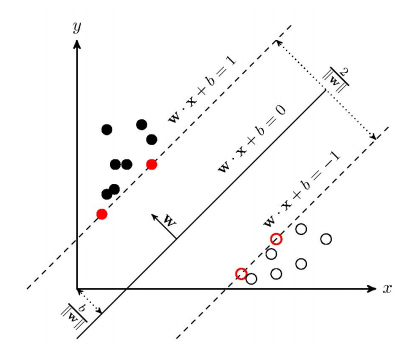
\includegraphics[scale=0.8]{\pref/svm.png}
    \caption{分离距离示意图.}
    \label{fig:svm}
\end{figure}

采样点$x_i$到分离超平面的归一化距离为
    $$\gamma_i=y_i\left(\left(\frac{w}{\norm{w}_2}\right)^\t x+\frac{b}{\norm{w}_2}\right).$$
$\gamma=\min_i\gamma_i$是最小的归一化距离. 于是我们的任务变成了最大化$\gamma$. 等价地,我们求解如下优化问题
\begin{align*}
    \max_{w,b}\quad&\gamma \\
    \text{s.t.}\quad&\gamma\le\gamma_i,\quad i=1,2,\dots,N.
\end{align*}

$\gamma\le\gamma_i$等价于$$y_i\left(\left(\frac{w}{\gamma\norm{w}_2}\right)^\t x+\frac{b}{\gamma\norm{w}_2}\right)\geq 1.$$
简洁起见,把$w$替换成$\frac{w}{\gamma\norm{w}_2}$,把$b$替换成$\frac{b}{\gamma\norm{w}_2}$,我们有$$y_i(w^\t x+b)\geq 1.$$
那么最大化$\gamma=\frac{1}{\norm{w}_2}$等价于最小化$\norm{w}_2^2$. 

我们得到以下凸规划问题:
\begin{align*}
    \min_{w,b}\quad&\frac{1}{2}\|w\|_2^2\\
    \text{s.t. }\quad &y_i(w^\t x_i+b)\geq 1,\quad i=1,2,\cdots, N.
\end{align*}

如何解决这个问题?利用上面的对偶理论,我们有如下步骤:
\begin{itemize}
    \item 第一步,用Lagrange乘子法,转化成Lagrange问题(min-max).
    \item 第二步,写出对偶问题(max-min),验证强对偶定理的正规性条件,于是只需要求解对偶规划.
    \item 第三步,写出KKT条件,将对偶规划解为一个二次规划(min) ,用优化算法求解二次规划.
\end{itemize}

\endgroup
\chapter{不动点理论}\label{chap:fixed-point-theory}

考虑优化算法$A$,它在函数$f$上的的收敛性如何?算法运行所产生的点列记为$\{x_n\}$,它满足$x_{n+1}=A(x_n)$. 如果关注序列$x_n$本身,那么这是一个数学分析的思路,通过寻找不同量之间的联系,来分析收敛性. 如果从算法$A$本身来看,这是一个算子法与泛函分析的思路,研究算法本身的性质,收敛性往往归结为吸收点的存在性. 后者是更加抽象且现代的思路。在本章中,我们将看到,从算子的角度来理解收敛性,最终问题就归结到了\emph{不动点理论}\index{不动点理论}。

不动点的定义是非常直接的,考虑一个集合$X$以及它到自身的映射$f:X\to X$,元素$a\in X$称为映射$f:X\to X$的\textbf{不动点}\index{不动点},如果$f(a)=a$. 本章将介绍三种不动点存在性定理。

\section{Banach不动点定理}
为了陈述不动点定理,我们需要引入一些数学概念。

\begin{definition}[度量与度量空间]\index{度量}\index{度量空间}\index{距离}
集合$X$上的\textbf{度量}(或\textbf{距离})$d$是映射
\[d:X\times X\to \R\]
满足条件
\begin{itemize}
\item 非负性:$d(x_1,x_2)\geq 0$,并且$d(x_1,x_2)=0\iff x_1=x_2$.
\item 对称性:$d(x_1,x_2)=d(x_2,x_1)$.
\item 三角不等式:$d(x_1,x_3)\le d(x_1,x_2)+d(x_2,x_3)$.
\end{itemize}
其中$x_1,x_2,x_3$是$X$的任意元素. 

此时,$(X,d)$或$X$被称为\textbf{度量空间}.
\end{definition}

下面给出一些度量的例子。
\begin{example}
    考虑实数集$\R$,要成为度量空间,可以装备以下度量:
    \begin{itemize}
            \item 平凡的离散度量:$\forall x_1\neq x_2\ d(x_1,x_2)\equiv 1, d(x,x)=0$. \index{度量!离散~}
            \item $d(x_1,x_2)=|x_1-x_2|$. \index{度量!绝对值~}
        \end{itemize}
        考虑向量空间$\R^n$,要成为度量空间,可以装备以下度量:
        \begin{itemize}
            \item Minkowski度量($L^p$度量):$d(x_1,x_2)=(\sum_{i=1}^n|x_1^i-x_2^i|^p)^{1/p}\ (p\ge 1)$. \index{度量!Minkowski~}\index{度量!$L^p$~}
            \item Manhattan度量($L^1$度量): $d(x_1,x_2)=\sum_{i=1}^n|x_1^i-x_2^i|$. \index{度量!Manhattan~}\index{度量!$L^1$~}
            \item Euclid度量($L^2$度量):$d(x_1,x_2)=\sqrt{\sum_{i=1}^n|x_1^i-x_2^i|^2}$. \index{度量!Euclid~}\index{度量!$L^2$~}
            \item Chebyshev度量($L^\infty$度量): $d(x_1,x_2)=\max_i|x_1^i-x_2^i|=\lim_{p\to\infty}(\sum_{i=1}^n|x_1^i-x_2^i|^p)^{1/p}$. \index{度量!Chebyshev~}\index{度量!$L^\infty$~}
        \end{itemize}
\end{example}

我们的目标是找到一类和实数集非常像的度量空间。实数集一个非常重要的性质是实数列收敛当且仅当它是Cauchy列。我们把这一性质抽象出来,就得到了如下定义:

\begin{example}
    度量空间$(X,d)$的点列$\{x_n:n\in \N\}$称为\textbf{Cauchy列}\index{Cauchy列},如果对于任何$\epsilon>0$,都可以找到序号$N\in\N$,使得对于任何大于$N$的序号$m,n\in\N$,$d(x_m,x_n)<\epsilon$成立.

    度量空间$(X,d)$称为\textbf{完备的}\index{完备空间},如果任意Cauchy列$\{x_n:n\in \N\}$都收敛:$\exists a\in X, \lim_{n\to\infty}d(a,x_n)=0.$
\end{example}
度量空间的任何收敛点列显然是Cauchy列,完备性本质上只是假设Cauchy收敛准则在该空间成立.

下面是一些完备度量空间的例子
\begin{example}
\begin{itemize}
\item $L^p$度量下下$\R^n$是完备的.
\item 使用度量$d(x_1,x_2)=|x_1-x_2|$,则$X=\R\setminus\{0\}$不是完备度量空间. 考虑$\{x_n=\frac1n:n\in\N\}$,它是Cauchy列,但该点列在$X$中没有极限(极限是$0$).

\item $[0,1]$到自身的连续函数空间$C([0,1])$在$L^\infty$度量下是完备的.
此时
\[d(f,g)=\sup_{x\in[0,1]}|f(x)-g(x)|,\]
完备性由一致收敛得到,函数空间是泛函分析中一个典型的研究对象.
\end{itemize}
\end{example}

下面我们给出与Banach不动点定理相关的概念:

\begin{definition}[压缩映射]
度量空间$(X,d)$到自身的映射$f:X\to X$称为\textbf{压缩映射}\index{压缩映射},如果存在$0<q<1$,使得不等式
    \[d(f(x_1),f(x_2))\le q\cdot d(x_1,x_2)\]
对于$X$中的任何两个点$x_1,x_2$都成立.
\end{definition}

用$\delta-\epsilon$语言容易证明压缩映射一定是连续映射:
\begin{lemma}\label{lemma:contraction-continuous}
    压缩映射$f:X\to X$是连续映射.
\end{lemma}

压缩映射一定有不动点,这就是Banach不动点定理:
\begin{theorem}[Banach不动点定理,压缩映像原理]\label{thm:banach-fixed-point}\index{不动点定理!Banach~}\index{压缩映射原理}

完备度量空间$(X,d)$到自身的压缩映射$f:X\to X$具有唯一的不动点$a$. 

此外,对于任何点$x_0\in X$,迭代序列$x_0,x_1=f(x_0),\cdots,x_{n+1}=f(x_n),\cdots$收敛到$a$. 收敛速度由以下估计给出:
\[d(a,x_n)\le \frac{q^n}{1-q}d(x_1,x_0).\]
\end{theorem}

\begin{proof}
首先证明存在性。$d(x_{n+1},x_n)\le qd(x_n,x_{n-1})\le \cdots\le q^nd(x_1,x_0).$
从而
\begin{align*}
d(x_{n+k},x_n)&\le d(x_n,x_{n+1})+\cdots+d(x_{n+k-1},x_{n+k})\\
&\leq(q^n+\dots+q^{n+k-1})d(x_1,x_0)\le \frac{q^{n}}{1-q}d(x_1,x_0).
\end{align*}
因此$\{x_n\}$是Cauchy列,存在极限$\lim_{n\to\infty} x_n=a\in X$.
结合压缩映射的连续性,有
$a=\lim_{n\to\infty}x_{n+1} = \lim_{n\to\infty}f(x_n)=f(\lim_{n\to\infty}x_n)=f(a).$

然后证明唯一性。若$f$还有其他不动点$a_1,a_2$,则
$0\le d(a_1,a_2)=d(f(a_1),f(a_2))\le qd(a_1,a_2).$
而这当且仅当$d(a_1,a_2)=0$,即$a_1=a_2$时才可能成立.
最后证明收敛速度. 对
$d(x_{n+k},x_n)\le \frac{q^n}{1-q}d(x_1,x_0).$
取$k\to\infty$,得到
$d(a,x_n)\le \frac{q^n}{1-q}d(x_1,x_0).$
\end{proof}

\begin{example}[落在地面上的地图]
将一座公园的地图铺开在公园地面上,则地面上恰有唯一一点与地图上对应的点重合. 设公园可以用有界的面闭区域$\Omega$表示. 设地图的压缩比是$\lambda\in(0,1)$. 现在固定一个平面直角坐标系,把地图铺在区域$\Omega$内,则从$\Omega$内的点$x$(公园中的地点)到地图上对应点$x'$的变换由下面的公式给出:
\[x' = f(x) := \lambda Rx + b.\]
其中$R$和$b$分别为旋转和平移变换. 

考虑$\norm{\lambda R}=\sup_{\norm{x}=1}\norm{\lambda Rx}=\lambda<1$,由Banach不动点定理可知,压缩映射$f(x)$有唯一不动点$a=f(a)$.
\end{example}

\begin{example}[梯度下降的收敛性]\index{梯度下降}
我们优化目标是寻找二阶可微凸函数$f(x),x\in \R^n$的最小值. 使用梯度下降方法:每次往最小梯度方向移动.
假设对任意$x\in \R^n$,
    \[L \le \lambda_{\min}(\nabla^2 f(x))\le \lambda_{\max}(\nabla^2 f(x))\le U.\]
    其中$\nabla^2f(x)$是$f$的Hessian矩阵(二次导数),$U\ge L>0$为给定的常数,$\lambda_{\min}(A),\lambda_{\max}(A)$表示矩阵$A$的最小、最大特征值.

我们要证明:梯度下降能收敛到最小值点,且具有指数收敛速度.

先看一下证明的思路,我们要设法证明梯度下降算法是完备度量空间中的一个压缩映射。首先,二阶可微凸函数的最小值点充分必要地满足$\nabla f(x)=0$. 其次,$\nabla f(x)=0 \iff x\in\R^n$是梯度下降算子$\mathcal T^{(\alpha)}$的不动点,其中$\mathcal T^{(\alpha)}: x\mapsto x - \alpha\nabla f(x)$, 这里$\alpha\in \R_+$为步长. 最后,$\mathcal T^{(\alpha)}$是一个完备度量空间的压缩映射,其压缩系数为$q(\alpha)=1-L\alpha$. 因此梯度下降可以收敛至唯一的最小值点,收敛速度可以由压缩系数估计.

为了使$q(\alpha)$确实一个压缩系数,我们需要$\alpha<\min L^{-1}$. $\mathcal T^{(\alpha)}$的不动点恰好满足$\nabla f(x)=0$,因此是最小值点. 我们只需要证明$\mathcal T^{(\alpha)}$是压缩映射,并给出压缩系数

由有限增量原理:
    \[\norm{\mathcal T^{(\alpha)}x - \mathcal T^{(\alpha)}y} \le \sup_{z\in[x,y]}\norm{I - \alpha \nabla^2 f(z)}_2\cdot\norm{x-y}_2.\]
    \item 最后,注意到$\norm{I-\alpha\nabla^2f(z)}_2$等于$I-\alpha\nabla^2f(z)$特征值的最大模,根据条件可知特征值的最大模 $\leq 1-L\alpha$.
\end{example}

\section{Brouwer不动点定理}
下面我们考虑更一般的度量空间中的不动点定理,为此我们需要引入\emph{连续映射}的概念。

\begin{definition}
设$X$和$Y$是度量空间$(X,d_X),(Y,d_Y)$,映射$f:X\to Y$在点$a\in X$\textbf{连续}\index{连续},指的是
    \[\forall\epsilon>0\exists\delta>0\forall x\in X(d_X(a,x) < \delta\Rightarrow d_Y(f(a),f(x))<\epsilon).\]
如果它在每个点$x\in X$连续,称$f$为\textbf{连续映射}\index{连续映射}. $X$到$Y$的连续映射的集合记为$C(X,Y)$. 
\end{definition}

当度量空间为欧氏空间时,连续映射的定义与欧氏空间中连续映射的定义相同. 接下来,我们还需要几个集合的概念。

\begin{definition}[开集、闭集和紧集]
    考虑度量空间$(X,d)$,$a\in X$的邻域$B(a,\delta):=\{x\in X|d(a,x)<\delta\}$.
\begin{itemize}
    \item 集合$G$是\textbf{开集}\index{开集}$G$指的是对于任何点$x\in G$,满足$B(x,\delta)\subset G$的邻域$B(x,\delta)$存在.
    \item 集合$F$是\textbf{闭集}\index{闭集},如果它的补集$X\setminus F$是$(X,d)$中的开集.
    \item 集合$K$是\textbf{紧集}\index{紧集},如果从$X$中任何覆盖$K$的开集族中可以选出有限个开集来覆盖$K$.
\end{itemize}
\end{definition}
当度量空间为欧氏空间时,开集和紧集的定义与欧氏空间中的定义相同,紧集等价于有界闭集. 后一条在一般的度量空间不一定成立!

有了上面的准备,我们就可以叙述Brouwer不动点定理了:

\begin{theorem}[Brouwer不动点定理]\index{不动点定理!Brouwer~}
    设$M\subset\R^n$是一个非空紧凸集,而$F:M\to M$是一个连续函数. 则存在$x\in M$使得$F(x)=x$成立.
\end{theorem}

Brouwer不动点定理可以通过该实际的例子来理解:将一张白纸平铺在桌面上,再将它揉成一团(不撕裂),放在原来白纸所在的地方,那么只要它不超出原来白纸平铺时的边界,那么白纸上一定有一点在水平方向上没有移动过. 这个断言依据Brouwer不动点定理在$\R^2$的情况,因为把纸揉皱是一个连续的变换过程.

另一个例子:大商场等地方可以看到的平面地图,上面标有“您在此处”的红点. 如果标注足够精确,那么这个点就是把实际地形映射到地图的连续函数的不动点.

下面我们看一个Brouwer不动点定理的应用例子。首先引入矩阵\textbf{不可约}的概念:对于$n$阶方阵$A$而言,如果存在一个置换矩阵(通过交换单位阵的列获得)$P$使得$P^\t AP$为一个分块上三角阵,我们就称矩阵$A$是\emph{可约的},否则就称该矩阵是\emph{不可约的}.\index{不可约矩阵}

\begin{theorem}[Perron-Frobenius定理]\index{Perron-Frobenius定理}
    设$A=(a_{ij})$为$n\times n$不可约实矩阵,所有元素均非负,$a_{ij}\ge 0$,则下列结论成立.
    \begin{itemize}
        \item 存在一个实特征值$r$,其他特征值$\lambda$的模均不超过$r$,即$|\lambda|\le r$.
        \item 存在一个与$r$对应的特征向量,其所有元素恒正.
        \item $\min_i\sum_{j}a_{ij}\le r\le \max_i\sum_j a_{ij}$.
    \end{itemize}
\end{theorem}


\begin{proof}
首先证明$A$存在一个正的特征值$r>0$. 考虑单纯形$S:=\{x\in\R^n|x\ge 0,\sum_i x_i=1\}$. 则$\forall x\in S$,有$Ax\ge 0$. 

断言$Ax>0$,若不然,$A$存在某一列全$0$(由$x\ge 0$和$A$非负可得). 此时可通过置换阵将该$0$列交换到第一列,则得到的矩阵为分块上三角,与不可约性矛盾.

可以在$S$上定义映射
\[T(x) = \frac1{\rho(x)}Ax,\]
其中$\rho(x) > 0$使得$T(x)\in S$.

显然$T(x)$是$S\to S$的连续映射. $S$是一个有界凸闭集. 由Brouwer不动点定理,存在$x_0\in S, x_0 = T(x_0)=\frac1{\rho(x_0)}Ax_0$.

令$r=\rho(x_0)$,则可得$r$为$A$的一个正的特征值.

我们接下来证明,与$r$对应的特征向量所有元素恒正. 由之前的证明,与$r$对应的特征向量$x_0\in S$,则$x_0\ge 0$. 我们证明$x_0>0$.

考虑$A = PBP^{-1}$,其中$P$是置换矩阵,则
\[PBP^{-1}x_0=rx_0\implies B(P^{-1}x_0)=r(P^{-1}x_0).\]

记$\tilde{x}_0 = P^{-1}x_0$.取$B$使得$\tilde{x}_0 = (\xi,0)^\t, \xi > 0$. 则
\begin{align*}
    \left(                 %左括号
        \begin{array}{cc}   
        B_{11} & B_{12}\\  
        B_{21} & B_{22}\\  
        \end{array}
    \right)
    \left(                 
        \begin{array}{c}   
        \xi\\  %第一行元素
        0\\
        \end{array}
    \right)=
    \left(                 
        \begin{array}{c}   
        r\xi\\  %第一行元素
        0\\
        \end{array}
    \right).
\end{align*}

此时$B_{21}\xi=0$,由$\xi>0$可得$B_{21}=0$. 这与不可约矛盾,因此$x_0 > 0$.

然后我们证明:若$\alpha$是$A$的任意特征值,有$|\alpha|\le r$. 设$0\le B\le A, By=\beta y$. 记$y^\star = |y|=(|y_i|)_i$. 于是有
\[|\beta|y^\star = |\beta y| = |By| \le By^\star\le Ay^\star.\]

由$A^\t$不可约,存在特征值$r_1>0$和特征向量$x_1>0, A^\t x_1 = r_1x_1$. 因此有
\[|\beta|x_1^\t y^\star \le x_1^\t Ay^\star = r_1x_1^\t y^\star.\]

由$x_1^\t y^\star>0$,则$|\beta|\le r_1$. 令$B=A$可得$|\alpha|\le r_1$,特别地$r\le r_1$. 同样有$r_1\le r$,故$r=r_1$. 

最后证明:
\[\min_i\sum_j a_{ij}\le r\le \max_i\sum_j a_{ij}.\]
以这样的方式获得$\tilde A$: 将$A$的每一行都扩增(不减小某个元素),使得每一行都达到$\max_i\sum_j a_{ij}$. 此时$\max_i\sum_j a_{ij}$成为$A$的一个正特征值,且特征向量$\tilde{x}_0=\frac 1n\cdot\mathbf{1}\in S$. 由之前的结论,假设$0\le A\le \tilde A$,可以得到$\tilde A$的正特征值$\tilde r\ge r$. 因此$r \le \max_i\sum_j a_{ij}$. 同理缩小$A$可得$\min_i\sum_j a_{ij}\le r$.
\end{proof}

Perron-Frobenius定理在Markov链中的有非常重要应用。回忆Markov链的平稳分布:满足矩阵方程$\pi = \pi P$和$\sum_i\pi_i=1$.  设该Markov链状态有限且对应的转移矩阵$P$是(非负实)不可约方阵. 由Perron-Frobenius定理,$P$存在一个特征值$1=\min_i\sum_ja_{ij}\le r\le\max_i\sum_j a_{ij}=1$,对应一个正特征向量$x_0\in S=\{x\in\R^n|x\ge 0,\sum_ix_i=1\}$. 因此不可约有限状态Markov链必然存在平稳遍历分布.


\section{不动点的一般视角}
    

\part{逻辑与博弈}\label{part:logic-game}
\chapter{动态博弈}\label{chap:dynamical-game}

本章我们讨论每个玩家需要操作多次的博弈,此时,博弈被称为\textbf{动态博弈}\index{博弈!动态~}.

\section{输赢博弈}

\textbf{输赢博弈}\index{博弈!输赢~}指的是玩家的收益只能取两个值(输或赢)的博弈. 赢博弈中,每个游戏状态只有一个玩家可以进行操作的情况研究最多. 这种情况通常称为\textbf{扩展式博弈}\index{博弈!扩展式~}. 围棋、象棋、斗地主都是输赢博弈. 输赢博弈的分类见\Cref{tab:win-lose-game}.

\begin{table}[ht]
    \centering
    \begin{tabular}{cc}
        二人 & 多人 \\
        输赢 & 输赢平\\
        有限深 & 无穷深 \\
        完全信息 & 不完全信息 \\
        非合作 & 合作
    \end{tabular}
    \caption{输赢博弈的分类.}
    \label{tab:win-lose-game}
\end{table}

\begin{example}
    斗地主是一个多人有限轮不完全信息合作输赢博弈.
\begin{figure}
    \centering
    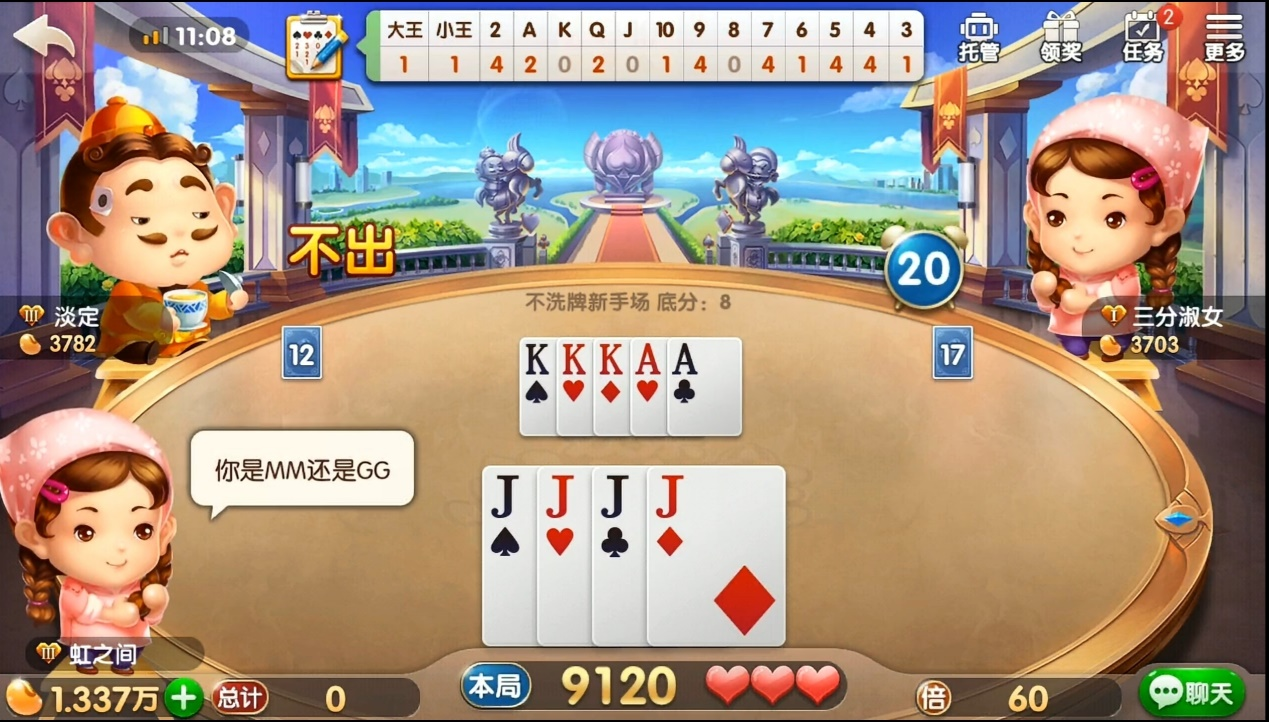
\includegraphics[width=0.75\textwidth]{Chapters/dynamical-game/figures/fight-landlord.jpg}
    \caption{斗地主.}
\end{figure}

\end{example}

我们在本部分主要关注最简单的一种博弈,即\emph{完全信息确定性回合制博弈}\index{博弈!完全信息确定性回合制~},与之相关的概念如下:
\begin{itemize}
    \item \emph{局面}\index{局面}:博弈的状态包括博弈本身的状态(棋盘状态、出牌情况等)和当前回合是哪个玩家.
    \item (无记忆)\emph{策略}\index{策略}:从局面到行动空间的映射$s_i:C\to\mathcal A$.
    \item \emph{确定性}\index{确定性}:给定当前格局和所有玩家的行动,可以唯一确定下一回合的格局.
    \item  \emph{完全信息}\index{完全信息}:所有玩家都知道当前局面,都知道每个玩家的行动,并且这些是共同知识.
\end{itemize}

这样的博弈可以用博弈树表示出来,例如,井字棋的博弈树见\Cref{fig:gametree}.

\begin{figure}
    \centering
    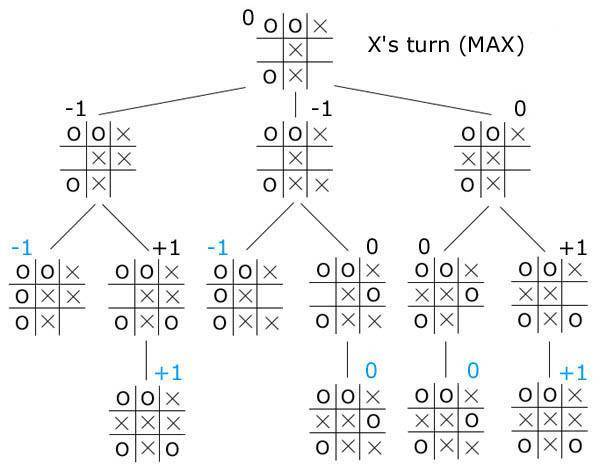
\includegraphics[scale=0.4]{Chapters/dynamical-game/figures/gametree.jpg}
    \caption{井字棋的博弈树.}
    \label{fig:gametree}
\end{figure}

输赢博弈一个自然的问题是:玩家是否总可以获胜?这就涉及到\emph{必胜策略}\index{必胜策略}的概念:无论对手如何进行行动,玩家都可以取得胜利的策略. 必胜策略是一种\emph{解概念}\index{解概念},即给定一个博弈,求解具有一定性质的玩家策略. 如果某个玩家具有必胜策略,那么我们就说这个博弈是\emph{被决定的}\index{博弈!被决定的~}. 什么博弈是被决定的?这一问题的答案由Zermelo定理给出.

\begin{theorem}[Zermelo定理, Von Neumann]\label{thm:zermelo}\index{Zermelo定理}
如果一个博弈是双人的、有限深的、确定的、完全信息的、输赢的,那么这个博弈是被决定的.
\end{theorem}
以上限定词缺一不可,缺少了任何一个都可能导致结论不成立.

\begin{proof}[证明一:逻辑证明]
设$W_i$表示“玩家$i$获胜”, $i=1,2$. 于是$x\in W_1\iff x\not\in W_2$.

先手玩家有必胜策略当且仅当
\[\exists a_0\forall b_0\exists a_1\forall b_1\dots\exists a_n\forall b_n: (a_0b_0\dots a_nb_n)\in W_1.\]

后手玩家有必胜策略当且仅当
\[\forall a_0\exists b_0\forall a_1\exists b_1\dots\forall a_n\exists b_n: (a_0b_0\dots a_nb_n)\in W_2.\]

两个命题互为否定,因此二者恰有一个成立!
\end{proof}

\begin{proof}[证明二:后向归纳法]
从博弈树的叶节点往根节点推理.

如果此节点是玩家$i$的回合,那么往后一轮的局面已经完全确定.
\begin{itemize}
    \item 如果有一种走法使得玩家$i$必胜,那么玩家$i$选择这种走法即可.
    \item 否则,玩家$i$无论如何也不可能获胜.
\end{itemize}

当到达到根节点的时候,有一方有必胜策略,另一方必输.

这种证明方式被称为\emph{后向归纳法}\index{后向归纳法}:从最后一期开始往前推理,最终确定一个解概念.
\end{proof}

如果博弈的结局还有平局,我们有如下Zermelo定理:
\begin{theorem}[有平局的Zermelo定理]\label{thm:zermelo-draw}\index{Zermelo定理}
如果一个博弈是双人的、有限深的、确定的、完全信息的,博弈的结果有输赢平局三种,那么下面三条有且仅有一条成立:
\begin{itemize}
    \item 第一个玩家有必胜策略.
    \item 第二个玩家有必胜策略.
    \item 双方都有不败策略,因此完全理性的玩家在博弈中必然平局.
\end{itemize}
\end{theorem}
证明留做练习。

尽管Zermelo定理的第二个证明构造出了必胜策略,但是后向归纳法的搜索空间过于庞大. 例如,充分大但有限的棋盘上,五子棋先手玩家存在不败策略,但是没有经过训练的人类或者简单的算法先手不一定会胜利。究其原因,人的思考以及机器搜索的过程实际上是前向探索的过程. 如何进行搜索是取得胜利重要的因素. 其中一个非常震撼的例子就是AlphaGo的出现,机器战胜了人类围棋高手. 以下我们介绍AlphaGo的设计思路.

由Zermelo定理可知,围棋也存在必胜策略. 然而标准围棋棋盘大小为$19\times 19$,状态空间量级为$10^{170}$,过大的状态空间使得我们无法使用后向归纳法求解出必胜策略. DeepMind的AlphaGo\index{AlphaGo}、AlphaZero\index{AlphaZero}利用深度强化学习的方法取得了围棋博弈的出色表现. 以下我们探讨AlphaGo如何通过神经网络建模博弈的过程.

AlphaGo算法包含\emph{策略网络}\index{策略网络}, \emph{价值网络}\index{价值网络}和\emph{Monte-Carlo树搜索}\index{Monte-Carlo树搜索}\index{MCTS}(MCTS).
\begin{itemize}
    \item 策略网络和价值网络的输入为当前局面状态$s\in C$. 
    \item 策略网络的输出为下一步落子位置$a\in\mathcal A$(361维的one-hot向量).
    \item 价值网络的输出为该局面的价值评估(期望收益: 输$-1$/赢$+1$).
    \item MCTS利用策略网络进行\emph{扩展},使用价值网络进行\emph{评估},利用UCB公式返回最优的搜索结果作为落子决策.
\end{itemize}

AlphaGo使用模仿学习(人类专家对弈数据)、强化学习(自博弈,策略梯度)的方式训练策略网络,使用自我博弈过程中的数据监督训练价值网络.

\lhysays{仔细讨论这部分{关于输赢博弈的讨论}
\begin{itemize}
    \item 什么叫完全理性的玩家?
    \item 表示完整的策略需要多少比特?
    \item 是否有高效的算法计算必胜策略?
    \item 如果博弈多方不是完全对抗的(即零和),那么是否还有必胜策略?是否有其他合理的解概念?
\end{itemize}}

我们再看一个有趣的例子:\emph{对话博弈}\index{博弈!对话~}。在对话博弈中,我们可以把对命题$\phi$的辩论过程形式化为一个博弈. 博弈中有两个玩家,一个需要证明$\phi$是真的,被称为\emph{正方} $P$,一个需要说明$P$的论据是有矛盾的,它被称为\emph{反方} $O$. 两个玩家可以对命题的某个部分发起\emph{质疑},或者对某个质疑作出\emph{辩护}. 当正方成功辩护了所有的质疑,而反方已经无法再发出新的质疑,正方获胜;否则反方获胜.

我们以命题逻辑为例,考虑合取和蕴含. 感叹号$!$表示陈述,问号$?$表示询问. 当一个玩家$X$($P$或者$O$)说了一个合取式,另一个玩家$Y$如果想质疑,需要询问合取中的某个部分($L^\wedge$或$R^\wedge$). $X$需要陈述该部分对应的命题作为辩护. 这一规则可以总结为\Cref{tab:dialogue-game-or}.
\begin{table}[ht]
    \centering
    \begin{tabular}{c|c|c}
         陈述&质疑&辩护  \\\hline
         $X!\varphi\wedge\psi$&$Y?L^\wedge$或$Y?R^\wedge$& 对应地,$X!\varphi$或$X!\psi$
    \end{tabular}
    \caption{对话博弈的规则:合取}
    \label{tab:dialogue-game-or}
\end{table}

当一个玩家$X$($P$或者$O$)说了一个蕴含式,另一个玩家$Y$如果想质疑,需要陈述前提. $X$则需要陈述结论作为辩护. 这一规则可以总结为\Cref{tab:dialogue-game-impl}.
\begin{table}[ht]
    \centering
    \begin{tabular}{c|c|c}
         陈述&质疑&辩护  \\\hline
         $X!\varphi\to\psi$&$Y!\varphi$&$X!\psi$
    \end{tabular}
    \caption{对话博弈的规则:蕴含}
    \label{tab:dialogue-game-impl}
\end{table}

我们考虑一个具体的例子$(p\wedge q)\to p$. 用一个表格来表示辩论的过程,这个表格有两列,分别表示玩家$O$和$P$. 每个玩家分别有三列,$A$表示当前操作是第几步(两个玩家统一计数),$B$表示当前操作质疑的是哪一步,中间一列表示当前的操作(陈述或者询问).
\[
    \begin{array}{|c|c|c|c|c|c|}
    \hline
        \multicolumn{3}{|c|}{O} & \multicolumn{3}{|c|}{P} \\\hline
        A &  & B & B & & A\\\hline\hline
    \end{array}
\]

\newcommand{\gray}{\cellcolor{gray}}
玩家$P$陈述要辩论的命题.
\[
    \begin{array}{|c|c|c|c|c|c|}
    \hline
        \multicolumn{3}{|c|}{O} & \multicolumn{3}{|c|}{P} \\\hline
        &&&&\gray !p\wedge q\to p&\gray 0\\
        \hline
    \end{array}
\]
玩家$O$质疑这一陈述.
\[
    \begin{array}{|c|c|c|c|c|c|}
    \hline
        \multicolumn{3}{|c|}{O} & \multicolumn{3}{|c|}{P} \\\hline
        &&&&!p\wedge q\to p&0\\\hline
        \gray 1&\gray !p\wedge q&\gray (0)&&&\\\hline
    \end{array}
\]
现在又一次轮到了玩家$P$,他可以选择为蕴含式辩护,或者质疑这个合取式. 我们假设他这次选择质疑合取式,那么他需要询问左边或者右边,假设他询问了左边:
\[
    \begin{array}{|c|c|c|c|c|c|}
    \hline
        \multicolumn{3}{|c|}{O} & \multicolumn{3}{|c|}{P} \\\hline
        &&&&!p\wedge q\to p&0\\\hline
        1&!p\wedge q& (0)&&&\\\hline
        &&&\gray (1)&\gray ? L^\wedge &\gray 2\\\hline
    \end{array}
\]
现在轮到了玩家$O$. 他已经没有别的可以进行的操作了,只能对操作$2$进行辩护.
\[
    \begin{array}{|c|c|c|c|c|c|}
    \hline
        \multicolumn{3}{|c|}{O} & \multicolumn{3}{|c|}{P} \\\hline
        &&&&!p\wedge q\to p&0\\\hline
        1&!p\wedge q& (0)&&&\\\hline
        \gray 3&\gray !p&\gray &(1)&? L^\wedge &2\\\hline
    \end{array}
\]
现在轮到了玩家$P$. 他已经没有别的可以进行的操作了,只能对操作$1$进行辩护. 因为玩家$O$已经陈述了$p$,所以他可以用这个陈述来辩护.
\[
    \begin{array}{|c|c|c|c|c|c|}
    \hline
        \multicolumn{3}{|c|}{O} & \multicolumn{3}{|c|}{P} \\\hline
        &&&&!p\wedge q\to p&0\\\hline
        1&!p\wedge q& (0)&\gray &\gray !p&\gray 4\\\hline
        3&!p&&(1)&? L^\wedge &2\\\hline
    \end{array}
\]
现在轮到了玩家$O$. 他已经不能操作了(没有可以质疑的,也没有可以辩护的),所以玩家$P$获胜.
\[
    \begin{array}{|c|c|c|c|c|c|}
    \hline
        \multicolumn{3}{|c|}{O} & \multicolumn{3}{|c|}{P} \\\hline
        &&&&!p\wedge q\to p&0\\\hline
        1&!p\wedge q& (0)&&!p&4\\\hline
        3&!p&&(1)&? L^\wedge &2\\\hline
    \end{array}
\]

我们还可以定义否定$\neg p$相关的辩论规则,留作练习. 

根据Zermelo定理,对话博弈一定有一人有必胜策略,我们还有更精细的定理:
\begin{theorem}\label{theorem:dialogue-game}
考虑对命题$\phi$的对话博弈,$\phi$是重言式当且仅当正方玩家$P$有必胜策略.
\end{theorem}

证明只需要考虑对$\phi$做归纳法. 实际上,我们如此规定对话博弈的规则,就是为了保证这一定理成立. 我们可以将一个命题真值的判定问题转化为玩家$P$博弈必胜策略的存在性问题,这对于一阶逻辑来说非常有用.


\section{随机博弈(Markov博弈)} %lhw
现在我们考虑无穷博弈中最简单的一种:\textbf{随机博弈}\index{博弈!随机~},也叫\textbf{Markov博弈}\index{博弈!Markov~}. 在随机博弈中,玩家的行动是随机的,但是玩家的行动空间是有限的. 为了简化问题,我们考虑两人随机博弈,即两个玩家轮流进行随机行动. 其相关概念如下:
\begin{itemize}
    \item 有限局面:$C=\{s_1,s_2,\cdots,s_N\}$.
    \item 有限策略:$\mathcal A=\mathcal A_1\times \mathcal A_2.$
    \begin{itemize}
        \item 每个局面具有自己的行动空间:$\mathcal A_p = \{\mathcal A_{p,1},\mathcal A_{p,2},\cdots, \mathcal A_{p,N}\}, (p=1,2)$.
        \item 每个行动空间有限:$|\mathcal A_{p,k}|=n_{p,k},(p=1,2;k=1,2,\cdots,N)$.
    \end{itemize}
    \item 在局面$s_k$, 若玩家1选择第$i$个行动$a_{1,k,i}(1\le i\le n_{1,k})$,玩家2选择第$j$个行动$a_{2,k,j}(1\le j\le n_{2,k})$,则
    
    \begin{itemize}
        \item 局面之间有转移概率:
        \begin{itemize}
            \item 该博弈以概率$s_{ij}^k$停止.
            \item 该博弈以概率$p_{ij}^{kl}$转移到状态$s_l$.
        \end{itemize}
        \item 收益:玩家1收获$Q(a_{1,k,i},a_{2,k,j};s_k)$,玩家2收获$-Q(a_{1,k,i},a_{2,k,j};s_k)$. 假设$Q$有界.
    \end{itemize}
\end{itemize}

随机博弈的过程如下。首先,博弈从某一个局面状态$s^0$开始,$s^0\in C$. 在每个阶段$t$,所有玩家同时选择自己的动作$a^t$. 环境根据所有玩家的动作$\boldsymbol a^t$和状态$s^t$,给予每个玩家对应的收益$q(\boldsymbol a^t, s^t)$,并转移到新的状态$s^{t+1}\in C$. 

假设在阶段$T$,所有玩家可以观察到所有历史动作$\{\boldsymbol a^t\}_{t\le T}$. 和一般的动态博弈一样,我们可以定义每个玩家的策略$\pi$——基于历史信息(状态、行动)到当前局面的行动的映射. 玩家在博弈的过程中,其实就是按照某个策略$\pi$进行行动的. 求解一个博弈也是求解最优策略$\pi_*$. 下面我们定义什么是``最优".

依赖历史信息的策略$\pi$一般很复杂. 由于收益只与当前局面、当前玩家的行动有关,我们可以缩小策略空间. 考虑第$p$个玩家($p=1,2$),定义\emph{平稳策略}\index{平稳策略}为$N$个概率分布:$\vec \pi_p=(\pi_p^1,\pi_p^2,\cdots,\pi_p^N)$,分别对应$N$个状态;每个概率分布$\pi_p^k=(\pi_{p,1}^k,\pi_{p,2}^k,\cdots,\pi_{p,n_{p,k}}^k)$,分别对应$|n_{p,k}|$个行动. 使用平稳策略时,无论博弈的历史轨迹如何,玩家$p$在状态$s_k$采取行动$a_{p,k,i}$的概率为$\pi_{p,i}^k$.

假设两个玩家分别用平稳策略$\pi_1,\pi_2$进行博弈,则从局面$s^0$开始的随机博弈中,第$p$个玩家($p=1,2$)的\emph{远期收益}\index{远期收益}:
        \[\Pi_p(\pi_1,\pi_2; s^0) = \E\left[\sum_{t=0}^\infty \gamma^t(-1)^{p-1} Q(\pi_1(s^t),\pi_2(s^t); {s^t}) \right].\]

以上定义容易扩展为一般随机博弈(多人、非零和). 随机博弈可以看做MDP的多人扩展$(N, C, \mathcal A, \mathcal P,\mathcal Q, \gamma)$:
\begin{itemize}
    \item $N$: 玩家的数量,$N=1$退化为MDP.
    \item $C$: 局面的集合.
    \item $\mathcal A$: 玩家的行动集合. $\mathcal A=\mathcal A^1\times \cdots\mathcal A^N$. 设$\mathcal A_i(s)$表示第$i$个玩家在状态$s$的行动空间.
    \item $\mathcal P: C\times \mathcal A\times C\to [0,1]$: 给定玩家的联合动作$\boldsymbol a\in\mathcal A$, 局面从状态$s\in C$转移到$s'\in C$的概率$P(s'|s,\boldsymbol a)$.
    \item $\mathcal Q: C\times \mathcal A\to \R$: 在状态$s$,当玩家的联合动作为$\boldsymbol a$时,玩家$i$的奖励值$Q_i(\boldsymbol a;s)$(有界). 
    \item $\gamma\in[0,1]$表示折扣系数,用于计算远期收益.
\end{itemize}

\emph{Markov完美均衡}(MPE)\index{Markov完美均衡}\index{MPE}是一种解概念. 求解博弈的过程中,我们限制所有玩家使用平稳策略. 此时,面对对手,玩家的最优策略被称为\emph{Markov最优反应}\index{最优反应}:对每个状态$s$,给定其他玩家的平稳策略$\pi_{-i}$,玩家$i$的行动$a_i\in \mathcal A_i(s)$最大化它的远期收益$\Pi_i(s;\pi_{-i})$:
    \[\Pi_i(s;\pi_{-i}) = \E\left[Q_i(a_i,\pi_{-i}(s);s) + \gamma\sum_{s'\in C} P(s'|a_i,\pi_{-i}(s),s)\Pi_i(s';\pi_{-i}) \right].\]

MPE被定义为:所有玩家的平稳策略组合,其中每个玩家的行动都是Markov最优反应。

我们可以类比MDP中求解最优价值的Bellman方程(动态规划)\index{MDP}\index{Bellman方程}的形式. 当假设其他玩家都使用平稳策略,对每个状态$s$,存在一个价值函数$V_i(s;\pi_{-i})$取得玩家$i$从$s$出发的最高远期收益,满足:
\begin{align*}
    V_i(s;\pi_{-i}) = \max_{a_i\in \mathcal A_i(s)}&\E[Q_i(a_i,\pi_{-i}(s);s) \\ &+ \gamma \sum_{s'\in C}P(s'|a_i,\pi_{-i}(s),s)V_i(s';\pi_{-i})].
\end{align*}

\begin{theorem}
    对于$N$个玩家、有限局面状态、有限动作空间的随机博弈,MPE存在.
\end{theorem}

下面我们介绍Shapley关于双人零和随机博弈情形的证明. 对于一般的情况,我们留做习题.

\newcommand{\val}{\mathsf{val}}
首先介绍一下\emph{矩阵博弈}\index{博弈!矩阵~}的概念. 假设$P$是一个$m\times n$的矩阵,玩家1有$m$种动作(动作集合$\mathcal A_1$),玩家2有$n$种动作(动作集合$\mathcal A_2$),元素$P_{ij}$表示双方采取动作$(i,j)$时玩家1的收益,玩家2的收益为$-P_{ij}$. 

回忆在不动点课程中的minimax定理\Cref{???}:
\[\val(P)=\max_{s_1\in \Delta(\mathcal A_1)}\min_{s_2\in\Delta(\mathcal A_2)}s_1^\T Ps_2=\min_{s_2\in \Delta(\mathcal A_2)}\max_{s_1\in\Delta(\mathcal A_1)}s_1^\T Ps_2.\]
$s_i$是玩家$i$的混合策略,$\Delta(\mathcal A_i)$表示玩家$i$所有混合策略的集合。$\val(P)$为矩阵$P$定义的\emph{矩阵博弈}的\emph{值}. 在任意Nash均衡中,玩家1的期望收益即为$\val(P)$. 下面我们将看到:双人零和随机博弈也存在值(即可定义均衡收益).

首先证明一个引理:
\begin{lemma}\label{lemma:matrix}
    对任意$m\times n$的矩阵$B,C$,成立:
    \[|\val(B)-\val(C)| \le \max_{i,j}|B_{ij} - C_{ij}|.\]
\end{lemma}

\begin{proof}
    设$(s_1,s_2)$为矩阵博弈B的Nash均衡,$(\bar{s}_1,\bar{s}_2)$为矩阵博弈C的Nash均衡. 于是由定义有:$s_1^\T B\bar{s}_2  \ge s_1^\T  B s_2$,且$\bar{s}_1 ^\T  C\bar{s}_2 \ge s_1^\T  C \bar{s}_2 $,因此
    \[s_1^\T  B s_2 - \bar{s}_1 ^\T  C\bar{s}_2  \le s_1^\T  B\bar{s}_2  - s_1^\T  C \bar{s}_2  \le \max_{i,j}|B_{ij} - C_{ij}|.\]
\end{proof}

下面,我们将矩阵博弈的概念迁移到随机博弈. 在双人零和的语境下,我们去掉收益函数$Q$的下标$i$. 定义\emph{值迭代}为以下过程:
\begin{itemize}
    \item 首先,我们选择一个任意的函数$\alpha: C\to \R$,其中C是局面的状态空间,称$\alpha$为\emph{值函数}(value function).
    \item 对任意$s\in C$,定义矩阵$R_s(\alpha)$为
    \[R_s(\alpha)(a_1,a_2) = Q(a_1,a_2;s) + \gamma \sum_{s'\in C}P(s'|a_1,a_2,s)\alpha(s').\]
    其中$a_1\in \mathcal A_1(s), a_2\in \mathcal A_2(s)$.
    \item 值函数从$\alpha_0$开始迭代,记$\alpha_k(s)=\val(R_s(\alpha_{k-1}))$. 
\end{itemize}
如何理解$\alpha_k(s)$? 假设选取$\alpha_0(s)\equiv 0$,则$R_s(\alpha_0)=Q(a_1,a_2;s)$是从$s$出发,由$Q$定义的矩阵博弈. $\alpha_1(s)=\val(R_s(\alpha_0))=\val(Q(\cdot,\cdot;s))$.

再看$R_s(\alpha_1)(a_1,a_2)=Q(a_1,a_2;s)+\gamma\sum_{s'\in C}P(s'|a_1,a_2,s)\alpha_1(s')$. 我们可以假想有一个被截断的两阶段随机博弈:
        \begin{itemize}
            \item 玩家在第一阶段从状态$s$出发,行动$(a_1,a_2)$待定;\item 在第二阶段,对于每个可能的状态$s'\in C$,玩家采用矩阵博弈$R_{s'}(\alpha_0)$的Nash均衡的行动.
        \end{itemize} 
博弈在第二阶段终止,远期收益累积的折扣部分为$\gamma \sum_{s'\in C}P(s'|a_1,a_2,s)\val(R_{s'}(\alpha_0))$. 从而,矩阵博弈$R_s(\alpha_1)$的值也是这个两阶段随机博弈的值. 更一般地,$\alpha_{k}(s)$是一个被截断的$k$阶段随机博弈的值.

为方便,我们定义迭代算子$(T\alpha)(s) = \val(R_s(\alpha))$.
        \begin{align*}
            \norm{T\alpha-T\alpha'}_\infty &= \max_{s\in C}|\val (R_s(\alpha)) - \val(R_s(\alpha'))| \\
            &\le \gamma \max_{s\in C} \max_{a_1,a_2}|\sum_{s'\in C}P(s'|a_1,a_2,s)(\alpha(s') - \alpha'(s'))| \\
            &\le \gamma \max_{s'\in C} |\alpha(s') - \alpha'(s')| \\
            &= \gamma \norm{\alpha-\alpha'}_\infty.
        \end{align*}
第一个不等式的成立使用了矩阵博弈值的不等式. 对于有折扣的博弈,$\gamma\in (0,1)$,因此$T$是一个压缩映射,由Banach不动点定理可知,$\alpha_k\to \alpha^*$满足$T\alpha^*=\alpha^*$.

考虑任意一个从$s$出发的双人零和随机博弈,在前$k$局的博弈中,玩家1采用最优策略,后续局面可选择任意动作. 由之前的分析可知,前$k$局构成的截断随机博弈远期收益为$\alpha_k(s)$. 而对于之后的博弈,玩家1损失的累积收益最差不超过$\gamma^k/(1-\gamma)\cdot \sup|Q|$. 因此,当$k\to\infty$时,玩家$1$的收益至少是$\alpha^*(s)$. 注意,这个下界是无视玩家2的行动得出来的.

另一方面,玩家2也可以确保自己的收益至少是$-\alpha^*(s)$. 由零和,因此均衡时玩家1的收益必定是$\alpha^*(s)$. 因此双人零和随机博弈的均衡收益(值)为$\alpha^*(s),s\in C$.

这样,我们就证明了MPE的存在性。

以上我们只说明了双人零和随机博弈的值存在,还没有指明最优策略如何取得. 类比矩阵博弈,我们有:
\begin{theorem}
$R_s(\alpha^*)$定义的矩阵博弈的最优策略$(\pi_1,\pi_2)$是随机博弈的MPE. 
\end{theorem}
\begin{proof}
固定玩家2的一个任意策略$\hat{\pi}_2$(不一定是平稳策略). 首先考虑一个$k$阶段截断博弈,我们定义$\alpha_0=\alpha^*$,可理解为,原博弈前$k$步动作待定,后面使用策略取得$\alpha^*$的远期收益.

在这个博弈中,玩家1可以无视玩家2的策略,确保至少取得$\alpha^*$的远期收益(已证明),因此若采用$\pi_1$也能取得:
\[\E\left[\sum_{t=0}^{k-1}\gamma^tQ(\pi_1(s^t),\hat{\pi}_2(s^t);s^t)+\gamma^k\alpha^*(s^k)\middle|s^0=s\right]\ge \alpha^*(s).\]
化简可得
\[\E\left[\sum_{t=0}^{k-1}\gamma^tQ(\pi_1(s^t),\hat{\pi}_2(s^t);s^t)\middle|s^0=s\right]\ge \alpha^*(s)-\gamma^k\norm{\alpha^*}_\infty.\]
因此
\[\Pi(\pi_1,\hat{\pi}_2;s)\ge \alpha^*(s) - \gamma^k\norm{\alpha^*}_\infty - \frac{\gamma^k}{1-\gamma}\sup|Q|.\]

同样地,令$k\to\infty$可得,上式R.H.S.趋于$\alpha^*(s)$. 对于玩家2的$\pi_2$证明对称,因此$(s_1,s_2)$是一个MPE.
\end{proof}

随机博弈在机器学习中对应着\emph{多智能体强化学习}(MARL),正如Markov决策过程对应着(单智能体)强化学习. MARL是多智能体系统(MAS)研究领域中的一个重要分支,它将强化学习技术、博弈论等应用到多智能体系统,使得多个智能体能在更高维且动态的真实场景中通过交互和决策完成更错综复杂的任务. 解MDP的过程是根据环境信息,优化决策,最大化远期收益,这是单智能体强化学习. 解随机博弈的过程,是在MDP的基础上引入多玩家,玩家有自己的效用函数,最大化自己的远期收益,这是多智能体强化学习. \index{多智能体强化学习}\index{MARL}\index{多智能体系统}\index{MAS}\index{强化学习}\index{MDP}

\chapter{静态博弈}\label{chap:static-game}
本章我们讨论静态博弈的基本概念和分析方法,并以此为基础,讨论博弈中认知相关的问题。

\section{正则形式博弈}
动态博弈通常被建模为\emph{\index{博弈!扩展形式~}扩展形式博弈}. 与之相对的是\emph{\index{博弈!正则形式~}正则形式博弈},即玩家只有一次行动的机会,所有玩家同时操作. 正则博弈通常要求信息是完全的. 这种博弈的过程与时间无关,属于\emph{\index{博弈!静态~}静态博弈}.


一个正则形式博弈有如下构成要素
\begin{itemize}
    \item 玩家集合:$I$,我们总是假设这是一个有限集合.
    \item 玩家的行动集(纯策略集):$A_i$,$i\in I$.
    \item 玩家的收益:$u_i:\prod_j A_j\to\R$.
    \item 完全信息:以上内容是所有玩家的共同知识.
\end{itemize}
所有人的策略拼在一起,即$s=(s_i)_{i\in I}$,构成博弈的\emph{\index{策略组合}策略组合}。有以下特殊的正则博弈:
\begin{itemize}
    \item 当$A_i$有限,我们称之为\emph{\index{博弈!矩阵~}矩阵博弈}.
    \item 当$A_i$和$u_i$都是连续的,我们称之为\emph{\index{博弈!连续~}连续博弈}.
    \item 当$\sum_i u_i=0$,我们称之为\emph{\index{博弈!零和~}零和博弈},
    当所有策略组合,收益和都是常数时,解概念的分析可以保持一致,我们也可以按零和处理. 
\end{itemize}

如何定义正则博弈的均衡?首先要明确均衡的概念。假设所有人之间是不能交流的,每个人独立做决策. 因此玩家之间不能协调彼此的决策. 因为只能行动一次,所以所谓\emph{均衡},指的是没有人对自己的决策感到后悔的状态,没有人可以通过改变自己现在的策略来获得更多的收益. 因此我们有如下定义:

\begin{definition}[Nash均衡]
(纯策略)\textbf{Nash均衡}指的是策略组合$s$,满足
    \[\forall i\in I\,\forall a_i\in A_i:u_i(s_i,s_{-i})\geq u_i(a_i,s_{-i}).\]
\end{definition}

我们也可以用不动点来理解Nash均衡。首先定义\emph{最优反应}\index{最优反应}:给定对手的策略$s_{-i}$,玩家$i$选择的最大化自己收益的策略$s_i$. Nash均衡的等价定义是每个人都达到了自己的最优反应,即最优反应的不动点.


\begin{example}[囚徒困境]\index{囚徒困境}
考虑一个经典的非合作博弈,\emph{囚徒困境}. 一共有两个玩家,行玩家和列玩家. 玩家的第一个选择是保持沉默,第二个选择是认罪并检举对方. 它有如下收益矩阵:
\[
\begin{pmatrix}
-1,-1&-10,0\\
0,-10&-5,-5\\
\end{pmatrix}.
\]
矩阵每一项第一个元素是行玩家的收益,第二个是列玩家的收益. 这个博弈有唯一的Nash均衡:每个人都认罪. 思考:打破Nash均衡的假设,有没有可能得到更好的结果?
\end{example}

然而,纯策略Nash均衡并不一定存在. 考虑如下的输赢(零和)博弈:猜硬币游戏\index{猜硬币游戏}. 行列玩家分别有一枚硬币,他们秘密地抛掷. 如果两个玩家的硬币上面相同,行玩家获胜;否则列玩家获胜. 收益矩阵为:
    \[
    \begin{pmatrix}
    1,0&0,1\\
    0,1&1,0\\
    \end{pmatrix}.
    \]
容易验证,这个博弈没有纯策略Nash均衡. 更一般地,二人正则输赢博弈中纯策略Nash均衡往往不存在. 我们有如下定理:
\begin{theorem}
设$G=(I,\{A_i\}_{i\in I}, \{u_i\}_{i\in I})$是一个二人正则输赢博弈,其中$I=\{1,2\}$. 那么,$G$存在纯策略Nash均衡当且仅当其中一个玩家存在必胜策略. % HW:证明这个定理的矩阵博弈形式
\end{theorem}
对比动态博弈中的Zermelo定理,静态的二人完全信息输赢博弈已经不能够保证必胜策略的存在性。因此,静态输赢博弈的结局往往比动态输赢博弈更加不确定. 我们可以利用这一事实去理解生成对抗网络模型的不稳定性.


\subsection{生成对抗网络}

\emph{\index{生成对抗网络}生成对抗网络}(GAN)\index{GAN} 有两个子模型组成,一个被称为\emph{\index{生成模型}生成模型},一个被称为\emph{\index{判别模型}判别模型}. 生成模型的任务是生成看似真实的数据,二判别模型的任务是识别给定的数据是真实的还是伪造的.

假设真实数据的分布为$F_{data}$. 生成模型为$G(x;\theta_g)$,参数为$\theta_g$,输入向量$x$,输出数据向量$z$. 当$x$服从分布$F_x$,$G$的输出会形成一个分布$F_g$. 判别模型为$D(z;\theta_d)$,参数为$\theta_d$,接受一个数据向量$z$,输出一个$[0,1]$中的实数,表示$z$来自分布$F_{data}$的概率. 我们假设$F_{data}$和$F_x$都是连续型分布,有密度函数$p_{data}$和$p_x$. 我们再假设$D$和$G$都是连续的.

将$G$和$D$看成两个玩家,于是GAN可以被看成一个二人零和博弈,收益函数为:
    \[
        V(G,D)=\E_{z\sim F_{data}}(\log D(z))+\E_{x\sim F_x}(\log(1-D(G(x)))).
    \]
$D$最大化$V$,$G$最小化$V$.

从博弈论角度出发,一个基本的问题是Nash均衡是否存在?假设$D$和$G$都可以任意选择连续函数. 我们将展示一种通用的方式求解连续博弈的Nash均衡. 注意到$G(x)$形成了一个连续分布,密度记为$p_g$.  首先证明密度函数存在性定理:
\begin{theorem}
设$X\sim \mathcal U(0,1)$. 对于任意密度函数$p$,存在一个连续函数$F$使得$F(X)$具有密度$p$.
\end{theorem}
\begin{proof}
设$F_p$是$p$对应的分布函数,它是一个单调的连续函数. 取$F(x)=\inf\{y\in \R: F_p(y)\geq x\}$即可.
\end{proof}
因此,$G$的行动等价于选择$p_g$.

给定$G$的选择$p_g$,我们来求$D$的最优反应$D^*$.
    \[V(G,D)=\int (p_{data}(x)\log D(x)+p_g(x)\log(1-D(x)))\d x.\]
函数$a\log x+b\log(1-x)$最大值在$x=a/(a+b)$的时候取得. 因此,
    \[D^*(x)=\frac{p_{data}(x)}{p_{data}(x)+p_g(x)}.\]
    
现在,给定最优反应$D^*=p_{data}(x)/(p_{data}(x)+p_g(x))$,我们来求$G$的最优反应. 直观上,$G$能做到的最好选择就是$p_g=p_{data}$. 此时,$D^*(x)=1/2$,因此对任意$G$,$V(G,D^*)=-\log 4$. $G$选任何策略都是一样的收益,因此这是一个Nash均衡. 我们证明了:
\begin{theorem}[GAN的Nash均衡存在性]
在GAN的博弈中,$G$选择$p_{data}$,$D$选择$1/2$是一个Nash均衡.
\end{theorem}

我们刚刚的分析过于理想化,需要考虑一些问题。首先,神经网络的大小是有限的,因此$G$不能选择任何$p_g$。因此,我们刚刚找到的Nash均衡可能不存在。其次,$p_{data}$是一个未知的量,我们只有一些样本。因此,$G$和$D$都需要一个算法来找到它们的最优策略。这就是训练GAN的过程。

我们接下来给出一种更符合实际的均衡概念。

\emph{\index{局部Nash均衡}局部Nash均衡}$(G^*, D^*)$是指在$G^*$和$D^*$的一个邻域内$(G^*, D^*)$形成了一个Nash均衡。\emph{\index{稳定局部Nash均衡}稳定局部Nash均衡}$(G^*, D^*)$是指$(G^*, D^*)$是一个局部Nash均衡,并且在$(G^*,D^*)$的一个邻域内,对任意$(G,D)$都有$V(G,D^*)\geq V(G,D)$和$V(G^*,D)\leq V(G,D)$。GAN的训练实际上就是在寻找稳定局部Nash均衡的过程。

稳定局部Nash均衡表明了,即便对手的策略具有(很小的)不确定性,玩家的策略依然是最优反应。在训练过程中,这样的不确定性很可能出现,源自精度或者误差. 因此,稳定局部Nash均衡是一个更有可能被找到的解,不稳定局部Nash均衡则很容易偏离. 然而,我们刚刚在理想条件下找到的Nash均衡其实也是不稳定的. 实际上,GAN的训练是一个非常不稳定的过程. 我们有如下结果:

\begin{theorem}
设GAN博弈的收益函数$V$是解析的,$(0,0)$是稳定局部Nash均衡,在$(0,0)$的一个邻域内,$V(G,D)=C+V^2f(V)+D^2g(D)+V^2D^2h(G,D)$,其中$f,g,h$都是解析函数,满足$f(0),g(0)\geq0 $,$C$是常数.
\end{theorem}

$V$要具备这种形式才可能有稳定局部Nash均衡. 然而一般的神经网络并不能具备这样的形式,所以很多情况下根本不存在稳定局部Nash均衡!

\subsection{混合策略}
我们已经看到,在相当普遍的情况下,纯策略Nash均衡并不存在. 所以我们需要允许玩家进行随机行动,这就是\textbf{混合策略}\index{混合策略}。混合策略就是建立在纯策略空间$S$上的一个概率分布. 混合策略空间记为$\Delta(S)$. 当$S$有$n$个元素(有限),$\Delta(S)$可以被表示为标准的$n$-单纯形:
    \[\Delta(S)=\left\{x\in\R^n:\sum_{i=1}^n x_i=1,x_j\geq 0,\forall j\right\}.\]

那么,有了混合策略,玩家的决策思考过程是怎么样的?一个非常标准的回答是\emph{期望效用理论}\index{期望效用理论},它由Von Neumann和Morgenstern提出. 该理论认为,在面对不确定性时,人按照期望效用进行决策. 因此,我们需要计算玩家的期望效用。为此,引入混合\emph{策略组合}\index{策略组合}:$\sigma=(\sigma_i)_{i\in I}$,其中$\sigma_i\in\Delta(A_i)$. $\sigma$是一个$(A_i)_{i\in I}$上的概率分布,每一维相互独立. 当所有玩家选定策略之后,玩家$i$的期望收益是:
    \[u_i(\sigma)=\E_{a\sim\sigma} u_i(a).\]


\begin{definition}[Nash均衡]\index{Nash均衡}
对于一个博弈$G=(I,\{A_i\}_{i\in I},\{u_i\}_{i\in I})$,混合策略Nash均衡$\sigma$满足对于任意玩家$i$和任意$\sigma_i'\in \Delta(A_i)$,都有
\[u_i(\sigma_i,\sigma_{-i})\geq u_i(\sigma_i',\sigma_{-i}).\]
\end{definition}
Nash著名的定理是:
\begin{theorem}[Nash均衡存在性定理]\index{Nash均衡存在性定理}
对于任意有限正则形式博弈,都存在一个混合策略Nash均衡.
\end{theorem}

我们来看一个例子。
\begin{example}
继续考虑猜硬币游戏\index{猜硬币游戏},收益矩阵为
\[
\begin{pmatrix}
1,0&0,1\\
0,1&1,0\\
\end{pmatrix}.
\]
容易证明,唯一的均衡是两个玩家都选择$(1/2,1/2)$.
\end{example}

尽管在数学上,混合策略是导出了漂亮的结果,但是混合策略并不是一个非常合理的概念. 如何理解混合策略?我们将在后面通过似然、知识论等方式来解释混合策略.


\section{不完全信息博弈(Bayes博弈)}

即便是纯策略Nash均衡也可能是不合理的状态. 考虑如下的二人博弈:
    \[\begin{pmatrix}
    1,1&0,0\\
    0,0&0,0
    \end{pmatrix}.\]
显然,两个人玩家都选择第二策略达到了Nash均衡. 然而,当行玩家对列玩家的选择有任意小的不确定性时,他都更倾向于选择第一个策略. 因此,我们给出的这个Nash均衡实际上描述了一种不太可能出现的状态. 这促使我们提出了所谓的\emph{颤抖的手完美化}\index{颤抖的手完美化}:$s$是一个纯策略Nash均衡,并且当对手玩家的策略有任何微小不确定性的时候,$s$中的策略依然是最优反应.

“颤抖的手”给了我们一个例子说明不确定性会影响玩家的决策. 那么如何量化不确定性?经济学的解决方案是\emph{Bayes解释}\index{Bayes解释}的概率论:每一个玩家对世界有一个先验的\emph{信念}\index{信念},信念在数学上被建模为对可能世界的概率分布.

利用这样的建模,我们可以给不完全信息博弈一个正式定义。一个不完全信息博弈有如下组成部分:
\begin{itemize}
\item 玩家集合:$I$.
\item 行动空间:$A=(A_i)_{i\in I}$,$A_i$表示玩家$A_i$的所有可能行动.
\item 类型空间:$\Theta=(\Theta_i)_{i\in I}$,$\Theta_i$表示玩家$i$的所有可能类型.
\item 收益函数:$u_i:A\times\Theta\to\R$,当所有人的行动和类型都确定的时候,玩家$i$能拿到的收益.
\end{itemize}
所有玩家的行动$a=(a_i)_{i\in I}$形成了一个行动组合. 所有玩家的类型$\theta=(\theta_i)_{i\in I}$形成了一个类型组合.

 $P_i\in\Delta(\Theta_i)$是玩家$i$类型的概率分布. $P_i$表示了其他玩家对玩家$i$类型的信念. 我们假设$P_i$是相互独立的,因此玩家$i$对其他玩家的信念是$P_{-i}=\prod_{j\neq i}P_j$. 玩家$i$知道自己的类型.

在使用这一定义的时候需要非常小心,在一般情况下,玩家$i$对这个世界的信念应该包含:
\begin{itemize}
    \item 其他玩家有谁;
    \item 自己和对手可能的行动;
    \item 自己的类型;
    \item 自己的收益函数;
    \item ……
\end{itemize}
然而,在上述标准的经济学模型中,我们做了如下严格的限制:
\begin{itemize}
    \item 玩家、可能行动、可能类型、收益函数是所有人的共同知识,没有人对这些东西有不一样的信念. 
    \item 玩家对世界的不确定性仅仅在于其他玩家的类型,而且所有人关于每个玩家类型的信念是一致且独立的.
    \item 自己的类型自己知道并且只有自己知道.
\end{itemize} 

下面我们看一个例子


\begin{example}[合作者]
考虑一个二人博弈,称为“工作-偷懒”博弈\index{博弈!工作-偷懒~}。两个人的行动都是“工作”($W$)或“偷懒”($S$)。行玩家的类型集合是单点集,列玩家的类型是“勤奋”($D$)或“懒惰”($L$)。收益矩阵为
\[\begin{array}{c|cc}
    \multicolumn{3}{l}{\theta_2=D,}\\
     &W&S  \\\hline
     W&3,3&-1,0\\
     S&2,1&0,0\\
\end{array}\qquad \begin{array}{c|cc}
    \multicolumn{3}{l}{\theta_2=L,}\\
     &W&S  \\\hline
     W&1,1&-1,2\\
     S&2,-1&0,0\\
\end{array}\]
\end{example}

在具有不确定性的世界中,玩家的策略如何定义?玩家如何决策?因为玩家知道自己的类型,但在决策的时候不能知道其他人的类型,所以一个完整的(纯)策略应该是$s_i:\Theta_i\to A_i$,即在给定自己的类型时,应该采取的行动.

关于收益,我们依然沿用期望效用理论. 当玩家$i$具有类型$\theta_i$,采取行动$a_i$,对手的策略是$s_{-i}$时,$i$的\emph{中期}期望收益为\index{中期收益}:
    \[\tilde u_i(a_i,\theta_i,s_{-i})=\E_{\theta_{-i}\sim P_{-i}}[u_i(a_i,s_{-i}(\theta_{-i}),\theta_i,\theta_{-i})].\]
利用期望效用理论,我们很容易定义均衡的概念:
\begin{definition}[Bayesian Nash均衡,BNE]\index{Bayesian Nash均衡}\index{BNE}
$s=(s_i)_{i\in I}$被称为\emph{Bayesian Nash均衡},如果
    \[\tilde u_i(s(\theta_i),\theta_i,s_{-i})\geq \tilde u_i(a_i,\theta_i,s_{-i})\]
对任意$i,\theta_i,a_i$都成立.
\end{definition}

我们也可以考虑\emph{前期}期望收益\index{前期收益},此时玩家$i$并不知道自己是什么类型,因此他也要对自己的类型求期望:
     \[\hat u_i(s_i,s_{-i})=\E_{\theta\sim P}[u_i(s_i(\theta_i),s_{-i}(\theta_{-i}),\theta_i,\theta_{-i})].\]
根据前期期望收益,我们也可以定义BNE为:
     \[\hat u_i(s_i,s_{-i})\geq u_i(s'_i,s_{-i})\]
对任意$i$和任意策略$s_i'$成立.

两个定义是等价的. 首先,前期期望收益是中期期望收益的加权平均. 然后,最大化前期期望收益等价于最大化平均中的每一项中期期望收益,也就是最大化中期收益. 所以这两者是等价的.

当所有的不确定性都消失的时候,我们得到的收益是真实的,被称为\emph{后期}收益\index{后期收益}. 前期、中期、后期分别表明了信息的确定程度.

\begin{remark}
    自然,我们也可以定义混合策略的BNE,此时策略$s_i$是一个$\Theta_i$到$\Delta(A_i)$的映射.
\end{remark}


\begin{example}[猜硬币游戏的BNE]\index{猜硬币游戏}
考虑猜硬币游戏:
\[
\begin{array}{c|cc}
    &H&T  \\\hline
    H&1,-1 &-1,1\\
    T&-1,1&1,-1\\
\end{array}
\]
如果两个人都出$H$的时候收益有微小的扰动,我们就得到了一个Bayes 博弈:
\[
\begin{array}{c|cc}
    &H&T  \\\hline
    H&1+\epsilon\theta_1,-1+\epsilon\theta_2 &-1,1\\
    T&-1,1&1,-1\\
\end{array}
\]
其中$\theta_i\sim\mathcal U[-1,1]$.

考虑策略:$s_i:[-1,1]\to\{H,T\}$满足
\[s_i(\theta_i)=\begin{cases}
H,&\theta_i\in[0,1],\\
T,&\theta_i\in[-1,0).
\end{cases}\]
容易证明,$(s_1,s_2)$是一个BNE. 
\end{example}

注意到,在上面的例子中,策略$(s_1,s_2)$导致的结果实际上是,每个玩家以等概率选择$H$和$T$. 当$\epsilon\to 0$,这个博弈收益矩阵回到了原始博弈. BNE形成的行动概率分布则趋于原始博弈的混合策略. 通过这样的办法,正则博弈的混合策略均衡被理解为:当不确定性趋于消失时候,BNE形成的行动概率分布. 这不是偶然的,实际上所有的正则博弈的混合策略均衡都可以用一系列(纯策略的)BNE\emph{纯化}.\index{纯化}

考虑一个正则博弈$(I,A,u)$. 给定一个扰动参数$\epsilon>0$,定义类型为$\theta=(\theta_i)_{i\in I}$,将收益扰动为:
\[\tilde u_i(s,\theta)=u_i(s)+\epsilon\theta_i,\quad\theta_i\in[-1,1].\]
假设$\theta_i\sim F_i$,相互独立,$F_i$是具有连续可微密度的分布. 如此就形成了一个\emph{扰动博弈}\index{博弈!扰动~}. 当扰动参数$\epsilon\to 0$时候,扰动博弈的BNE趋于正则博弈的混合策略均衡,这正是下面的\emph{Harsanyi纯化定理}\index{Harsanyi纯化定理}。

\begin{theorem}[Harsanyi纯化定理]\label{thm:har}\index{Harsanyi纯化定理}
给定玩家集$I$和行动空间$A$. 对于一般的收益函数$u$和连续分布族$\{F_i\}_{i\in I}$,对任意完全信息正则博弈$(I,A,u)$的混合策略Nash均衡$\sigma$,存在一列扰动博弈纯策略BNE $s_\epsilon$,当扰动参数$\epsilon\to 0$,$s_\epsilon\to \sigma$.
\end{theorem}
混合策略均衡可以被看作不确定性趋于消失的时候的纯策略均衡. 这一定理的原始证明需要用到Brouwer不动点定理和隐函数定理,并且比较长,这里略去.

人们常说
\begin{quotation}
``Decision makers do not flip coins in the real world.''
\end{quotation}

然而,如果玩家对收益的信念有微小的不确定性的时候,他的行为就仿佛在抛硬币. 这是混合策略的似然解释(主观概率论).

\lhysays{细化这一部分。
{混合策略的进一步讨论}
\begin{itemize}
    \item 我们之前说过,Bayes博弈对于玩家信念的刻画是相当受限制的.
    \begin{itemize}
        \item 当引入不确定性、知识、信念的概念的时候,几乎不可避免需要加入限制条件.
    \end{itemize}
    \item 另一方面,概率论的Bayes学派解释在哲学上也有很多争议.
    \begin{itemize}
        \item 一旦使用Bayes学派的概率论研究不确定性、知识、信念,这一问题也是不可避免的.
    \end{itemize}
    \item 因而,我们可以考虑完全理性、完全耐心玩家在无穷轮重复的完全信息博弈中的决策行为.
    \begin{itemize}
        \item 玩家做出行动$a$的极限频率就是行动$a$在混合策略中的概率.
    \end{itemize}
    \item 这一角度并不涉及不确定性、信念等数学上模糊的概念,单纯讨论混合均衡达到的方式.
\end{itemize}
}

\part{认知逻辑}\label{part:cognitive-logic}
\chapter{模态逻辑基础}\label{chap:modal-logic}
\chapter{认知逻辑与共同知识}\label{chap:epistemic-logic}

\begingroup
\newcommand{\pref}{Chapters/epistemic-logic/figures}

\section{“泥泞的孩童”谜题}
有$n$个孩子在玩泥巴,他们互相泼泥巴. 母亲告诉孩子们,如果他们脸上沾上了泥巴,会受到严厉的惩罚. 孩子们不能看到自己的脸,但是可以看到其他所有人的脸. 所有孩子都希望保持自己的脸干净,但是弄脏别人的脸. 此时,孩子的父亲出现了,于是,孩子们停止泼泥巴. 孩子们互相不说话. 父亲看到了$k$($k\geq 1$)个人脸上有泥巴,于是宣布:“\emph{你们至少有一个人脸上沾了泥巴.}” 之后,父亲会公开地问若干轮如下问题: “\emph{你们知道自己脸上有泥巴了吗?}” 孩子们回答“知道”或者“不知道”. 假设孩子们观察力敏锐、聪慧且诚实,并且每一轮他们都同时回答. 接下来会发生什么?

假设有$k$个孩子脸上有泥巴. 谜底:在前$k-1$轮中,所有孩子都会说“不知道”,在第$k$轮中,所有脸上有泥巴的孩子都会说“知道”. 这一结论的论证来源于对$k$的归纳.

当$k=1$时,脸上沾满泥巴的孩子看到其他人都没有泥巴. 既然他知道至少有一个孩子的脸上有泥巴,他就能推出那个人肯定是他自己. 

现在假设$k=2$,脸上沾满泥巴的孩子是$a$和$b$. 一开始,因为他们分别看到了对方的脸上有泥巴,所以他们每个人都回答“不知道”. 但是,当$b$回答“不知道”时,$a$意识到他自己肯定是脸上有泥巴的那个孩子,否则$b$就会在第一轮中知道泥巴在他的脸上,并回答“知道”. 因此,$a$在第二轮回答“知道”. $b$也会通过同样的推理得出相同的结论. 

 现在假设$k=3$,脸上沾满泥巴的孩子分别是$a$,$b$和$c$. 孩子$a$的论证如下. 假设我没有泥巴落在脸上. 根据$k=2$的情况,$b$和$c$在第二轮都会回答“是”. 他们没有这样做,我意识到假设是错误的,我的脸上也有泥巴. 因此在第三轮我会回答“知道”. $b$和$c$的论证也是类似的.

$k=3$的论证具有一般性,对一般的$k$也成立.

\begin{remark}
“泥泞的孩童”还有其他流行的陈述方式,比如“蓝眼睛红眼睛”. 一个岛上有100个人,其中有5个红眼睛,95个蓝眼睛. 这个岛有三个奇怪的宗教规则.
    \begin{enumerate}
        \item 他们不能照镜子,不能看自己眼睛的颜色. 
        \item 他们不能告诉别人对方的眼睛是什么颜色. 
        \item 一旦有人知道了自己的眼睛是红色,他就必须在当天夜里自杀.
    \end{enumerate}
岛民不知道具体有几个红眼睛. 

某天,有个旅行者到了这个岛上. 由于不知道这里的规矩,所以他在和全岛人一起狂欢的时候,一不留神说了一句话:“\emph{你们这里有红眼睛的人. }”假设这个岛上的人足够聪明,每个人都可以做出缜密的逻辑推理. 请问这个岛上将会发生什么?
\end{remark}

那么,为什么会这样呢?如果$k>1$,那么所有人都知道$p$:“至少有一个人脸上有泥巴”. 那么父亲说这句话的意义是什么?如果父亲没有说$p$,那么会发生什么?无论父亲问多少轮,所有孩子都只会回答“不知道”!(为什么)因此,父亲公开说了$p$,这是谜题的关键.

假设$k=2$,脸上沾满泥巴的孩子是$a$和$b$. 在父亲宣布$p$之前,$a$和$b$都知道$p$. 然而,他们并不知道对方知道$p$. $a$可能会有两种想法:
    \begin{itemize}
        \item 我的脸上有泥巴,所以$b$知道$p$.
        \item 我的脸上没有泥巴,$b$是唯一一个有泥巴的,所以$b$不知道$p$.
    \end{itemize}
当父亲宣布$p$之后,$a$知道了$b$知道$p$. 当第一轮$b$回答“不知道”之后,$a$可以用“$b$知道$p$”这一知识推出自己脸上有泥巴.

假设$k=3$,脸上沾满泥巴的孩子是$a$,$b$和$c$. 在父亲宣布$p$之前,$a$,$b$和$c$不仅知道$p$,而且知道彼此知道$p$. 以$a$的视角看,$b$能看到$c$脸上有泥巴,所以$a$知道$b$知道$p$. 但是,$a$,$b$,$c$都不知道所有人知道所有人知道$p$!


用$E^m p$表示所有人知道所有人知道……所有人知道($m$次)$p$. 在一般情况下,父亲没有宣布$p$之前,$E^k p$并不成立. 父亲宣布了$p$之后,对任意$m\geq 1$,$E^m p$都成立!因此,父亲宣布$p$带来了\emph{共同知识}\index{共同知识}. 有了共同知识,这一谜题就可以按照我们所讨论的方式进行下去.

我们曾经假设过所有人“观察力敏锐、聪慧且诚实”. 然而,这一假设并不足够. 我们必须假设所有人都知道所有人“观察力敏锐、聪慧且诚实”,所有人都知道所有人都知道所有人“观察力敏锐、聪慧且诚实”,……换言之,我们需要假设“所有人观察力敏锐、聪慧且诚实”是共同知识. 假设还是只有两个孩子$a,b$脸上有泥巴. 假如$a$不知道$b$是诚实的,即便$b$回答了“不知道”,$a$也无法从$b$的回答中得到任何额外的知识!

除了假设“所有人观察力敏锐、聪慧且诚实”是共同知识,我们还需要假设以下陈述是共同知识:
    \begin{itemize}
        \item 每个人都能看到所有除自己外的人.
        \item 每个人都听到了父亲说的话.
        \item 父亲是诚实的.
        \item 每个人都在每一轮进行了充分的推理.
        \item ……
    \end{itemize}
任何假设的破坏都会导致之前的讨论失效. 那么,为什么父亲宣布$p$就可以让$p$变成共同知识呢?

所有人都\emph{听到}父亲说$p$并不能产生共同知识. 假如父亲只是对每一个孩子单独宣布$p$. 所有人并不知道所有人都知道$p$,因而仅仅可以做到$E p$. 那么,所有人都\emph{知道}所有人听到父亲说$p$会如何呢?进一步假设每个孩子给每一个孩子都安装了窃听器,每个人都能够偷听每个人与父亲的谈话内容. 所有人并不知道所有人都知道所有人都知道$p$,因而仅仅有$E^2 p$. 因此,父亲宣布$p$会产生共同知识的核心原因是\emph{公开宣布},此时对每一个$m$都有$E^m p$.

“泥泞的孩童”谜题足以表明,关于“知道”的讨论远比想象的复杂. 关于“知道”和知识的研究在哲学中划归为\emph{知识论}\index{知识论}. 接下来,我们将使用模态逻辑来形式化关于“知道”和知识的讨论,这被称之为\emph{认知逻辑}\index{认知逻辑}.


\section{认知逻辑的基本模型与性质}

假设有$n$个人,分别叫$1,2,\dots,n$. 基本命题集为$\mathbf P$,用字母$p,q,r,\dots$表示基本命题,例如,$p$表示“孩子$1$的脸上有泥巴”. 回忆:逻辑框架是一个三元组(语言,模型,语义). 命题认知逻辑的的三元组是:
\begin{itemize}
    \item 语言$L_n$:命题逻辑加上模态算子$K_i,i=1,\dots,n$.
    \item 模型$\mathcal M,w$:Kripke模型
    \item 语义$\vDash$:可能世界语义
\end{itemize}

模态公式$K_i\phi$被读作“$i$知道$\phi$”. 从语义来说,$K_i$是$\Box$算子,即我知道$\phi$意味着在我认为的所有可能世界中$\phi$都是真的,因此,$\mathcal M,w\vDash K_i\phi$当且仅当对任意$v$,如果$w\to_i v$,那么$\mathcal M,v\vDash\phi$.

模态公式的真值有两个层面,一个是在点模型上可满足:$\mathcal M,w\vDash\phi$,另一个是在框架上有效:$\mathcal F\vDash\phi$.

虽然我们没有定义$K_i$的对偶算子,但是$K_i$的对偶相当于$\Diamond$算子. $\neg K_i\neg\phi$表示的意思是“$i$不知道$\phi$不是真的”,因此$i$会考虑$\phi$可能是真的. 当然,这也意味着$i$会考虑$\neg\phi$也可能是真的. 例如考虑“我不知道上帝存在”和“我知道上帝不存在”,他们的模态公式分别是$\neg Kp$和$K\neg p$. 显然,前者是更弱的一种表述,因此$\neg K$和$K\neg$的含义完全不同.

\begin{example}
\begin{itemize}
    \item $K_1K_2p\wedge \neg K_2K_1K_2 p$.
    
    $1$知道$2$知道$p$,但是$2$并不知道$1$知道$2$知道$p$.
    
    \item $\neg K_i p\to K_i(\neg K_i p)$.
    
    如果我不知道$p$,那么我知道我不知道$p$.
    
    \item $K_i(p\wedge\neg K_i p)$.
    
    我知道如下的陈述:$p$是真的,且我不知道$p$. 一种类似的写法是,$K_ip\wedge K_i\neg K_ip$. 我知道$p$,但是我又知道我不知道$p$.
\end{itemize}
\end{example}

模态算子$K_i$有特殊的性质,这要求我们对$K_i$对应的关系$R_i$也有额外的要求. 我们要求每一个$R_i$都是等价关系$\sim_i$:
    \begin{itemize}
        \item 自反:$\forall x\, x\sim_ix$.
        \item 传递:$\forall x,y,z(x\sim_iy\wedge y\sim_iz)\to x\sim_iz$.
        \item 对称:$\forall x,y(x \sim_i y\leftrightarrow y\sim_ix)$.
    \end{itemize}
从可能世界的角度来说,这一要求就是说对$i$来说,她所认为可能的世界之间都是不可区分的.

从模态可定义性的角度来说,$R_i$的特殊性质会对应$K_i$特殊的公式. 这些公式就可以被看成关于“知道”的公理(模式)或推导规则. 承认某一条公理(模式)或推导规则就必须承认可能世界具有某一种性质,反之亦然.

\begin{axiom}[分配公理]\index{分配公理}
    $\vDash (K_i(\phi\to\psi)\wedge K_i\phi)\to K_i\psi$.
\end{axiom}
有效性验证如下:假设$\mathcal M,w\vDash K_i(\phi\to\psi)$且$\mathcal M,w\vDash K_i \phi$. 于是,对所有$R_i$后继$v$都有$\mathcal M,v\vDash\phi\to\psi$和$\mathcal M,v\vDash\phi$,因而$\mathcal M,v\vDash\psi$. 根据定义,$\mathcal M,w\vDash K_i\psi$,因而对所有$\mathcal F$,分配公理有效.

分配公理类比演绎推理的肯定前件(MP)推导规则. 分配公理意味着拥有知识的个体可以对自己的知识做任意的演绎推理,因而假设个体是\emph{逻辑全知}\index{逻辑全知}的.

\begin{principle}[知识泛化规则]\index{知识泛化规则}
    对所有$\mathcal F$,如果$\mathcal F\vDash\phi$,那么$\mathcal F\vDash K_i\phi$.
\end{principle}
有效性验证如下:假设$\mathcal F\vDash\phi$,这意味着对所有基于$\mathcal F$的点模型都有$\mathcal M,w\vDash\phi$. 因此,对任意$w$的$R_i$后继$v$,也有$\mathcal M,v\vDash\phi$. 所以也有$\mathcal M,w\vDash K_i\phi$成立,因而$\mathcal F\vDash K_i\phi$.

知识泛化规则类比一阶逻辑推理的泛化规则. 前提成立的$\phi$是关于$\mathcal F$本身的性质(特别是关于知识),因此知识泛化规则意味着个体知道关于知识的一切性质. 其实更重要的是,知识的一切性质都是共同知识.% HW


\begin{axiom}[知识公理或真理公理]\index{知识公理}\index{真理公理}
    $\vDash K_i\phi\to\phi$.
\end{axiom}
验证留作练习. 知识公理意味着,$i$知道的命题一定是真的. 在知识论中,这一要求实际上反映了“拥有知识”需要付出努力、值得一定的奖励. 与此相对应地,\emph{信念}\index{信念}则是更加主观、随意的,因而并不具有真理性. 为了理解这一点,对比以下两句话:我考试挂了,但不知道我考试挂了;我考试挂了,但我不相信我考试挂了.

\begin{axiom}[正内省公理]\index{正内省公理}
    $\vDash K_i\phi\to K_iK_i\phi$.
\end{axiom}

\begin{axiom}[负内省公理]\index{负内省公理}
    $\vDash \neg K_i\phi\to K_i\neg K_i\phi$.
\end{axiom}

验证留作练习.  这两条公理意味着个体会通过内省来知道自己的处境,特别是“我知道什么”和“我不知道什么”. “知之为知之,不知为不知”. 这里留一个思考:(负)内省公理是否合理?

以上五条性质(四条公理+一条推导规则)加上MP形成的推理系统称为\emph{S5公理系统}\index{S5公理系统}. 需要注意的是,这些公理其实都是公理模式,包含了无穷条公理. 此外,从哲学的角度讨论,还有一些别的公理,例如
\begin{axiom}[一致性公理]
    $\vDash_H\neg K_i\bot$.
\end{axiom}
这一公理表明个体不能够知道假的陈述,以此区别于信念.

我们基于框架类$H$给出了关于知识的公理. 反过来,公理对应什么样的框架结构呢?我们总结在\Cref{tab:knowledge-axiom-frame}中.
    \begin{table}[ht]
        \centering
       \begin{tabular}{cc}
\toprule 公理 &  $R_i$的性质 \\
\midrule $K_i \varphi \to \varphi$ & 自反性 \\
$K_i \varphi \to K_i K_i \varphi$ & 传递性 \\
$\neg K_i \varphi \to K_i \neg K_i \varphi$ & 欧氏性 \\
$\neg K_i\bot$  & 序列性\\
$\varphi \to K_i \neg K_i \neg \varphi$ & 对称性 \\
\bottomrule
\end{tabular}
        \caption{知识公理对应的模型结构}
        \label{tab:knowledge-axiom-frame}
    \end{table}

这里,欧氏性的定义如下:
\[\forall x,y,z(xR_iy\wedge xR_iz\to yR_iz).\]
直观上说,欧氏性意味着关系一定形成三角形.

序列性定义如下:
\[\forall x\exists y\, xR_iy.\]
换言之,所有点都有后继. 这里留两个思考. 从可能世界角度,$R_i$的这些性质有什么直观的含义?为什么有些公理没有对应的结构性质?(提示:注意观察一个公理/规则是否有$H$出现)

可以看出来,以上关系其实并不是孤立的,我们有:
\begin{lemma} %HW
\begin{itemize}
    \item 如果$R_i$是自反和欧氏的,那么$R_i$是对称和传递的.
    \item 如果$R_i$是对称和传递的,那么$R_i$是欧氏的.
    \item 以下命题等价:
    \begin{itemize}
        \item $R_i$是自反、对称和传递的.
\item  $R_i$是对称、传递和序列的.
\item $R_i$是自反和欧氏的.
    \end{itemize}
\end{itemize}
\end{lemma}
证明留作练习.

下面我们将认知逻辑语言加入共同知识算子和它的语义. 首先加入“所有人都知道”这个算子:$E\phi\leftrightarrow\bigwedge_i K_i\phi$. 记$E^k\phi$为$\underbrace{E\dots E}_k\phi$. 于是,共同知识算子$C$的语义定义为:
    \[\mathcal M,w\vDash C\phi\iff\mathcal M,w\vDash E^k\phi,\quad k=1,2,\dots\]

我们可以从图结构来理解共同知识算子. $\mathcal M,w\vDash E^k\phi$的含义是,从$w$出发走$k$步可到达的可能世界$v$上都有$\mathcal M,v\vDash \phi$. $\mathcal M,w\vDash C\phi$的含义则是,从$w$出发可到达的可能世界$v$上都有$\mathcal M,v\vDash \phi$.

类似算子$K_i$,$C$也有它对应的公理和推导规则.
\begin{axiom}[不动点公理]\index{不动点公理}
    $\vDash C\phi\leftrightarrow E(\phi\wedge C\phi)$.
\end{axiom}
共同知识是一个递归方程的(最小)解,这是一种不动点的视角.

\begin{principle}[归纳规则]\index{归纳规则}
    如果$\mathcal F\vDash \phi\to E(\phi\wedge\psi)$,那么$\mathcal  F\vDash \phi\to C\psi$.    
\end{principle}

每个人都可以从真实中得到的知识,一定是共同知识. 将S5公理系统中加入关于$E$和$C$的公理,我们就扩展了认知逻辑. 因为$E$和$C$是用$K_i$定义的,因此他们本身并不会带来Kripke模型新的结构性质.

\subsection{“泥泞的孩童”再回顾}

现在,我们可以形式化、严格讨论“泥泞的孩童”这一谜题了. 这一问题对应的逻辑语言是认知逻辑语言. 可能世界是$\{0,1\}^n$的元素$x=(x_1,\dots,x_n)$,$x_i=1$表示孩子$i$脸上有泥巴,$x_i=0$表示$i$脸上没有泥巴. 假设每个孩童$i$对应的$R_i$都是一个等价关系. 当我们如此假设时,每个孩子唯一不是共同知识的事情就是脸上泥巴的状态,其他的所有事情都被隐含在了共同知识之中.

原子命题$p_i$表示孩子$i$脸上有泥巴,$p$表示至少有一个孩子脸上有泥巴. 假设现在父亲还没有说出$p$. 对于孩子$i$,他的认知中只有两个可能世界:我的脸上有泥巴,或者我的脸上没有泥巴,其他对他来说都是确定的. 因此,$x R_i y$当且仅当$x_j=y_j$对任意$j\neq i$成立.于是,框架$\mathcal F$会对应一个$n$维超立方体. $n=3$的例子见\Cref{fig:cubic-example}.

\begin{figure}[ht]
    \centering
    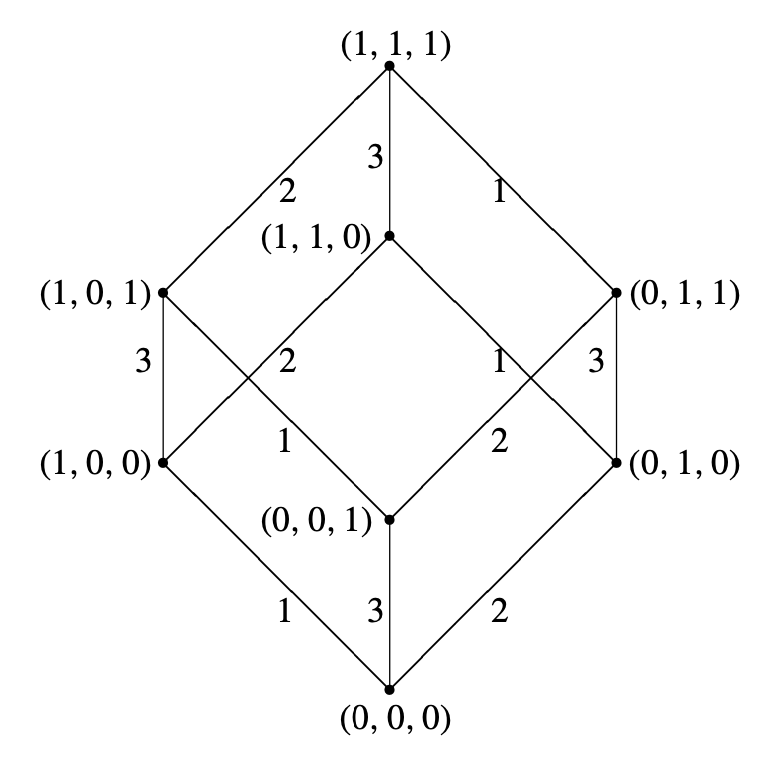
\includegraphics[scale=0.4]{\pref/cubic-example.png}
    \caption{$n=3$的情况}
    \label{fig:cubic-example}
\end{figure}

从框架$\mathcal F$到模型$\mathcal M$,我们还需要确定赋值$V$. $w\in V(p_i)$当且仅当$w_i=1$. $w\in V(p)$当且仅当所有分量$w_j$不全为零. 从模型到点模型,我们还需要确定我们所处的可能世界,于是我们就可以讨论模态公式的可满足性. 例如:$\mathcal M,(1,0,1)\vDash Ep$,但是$\mathcal M,(1,0,1)\vDash \neg E^2p$. 

假设现在父亲宣布了$p$,那么$\mathcal F$将会去掉$0$这个点,见\Cref{fig:cubic-example-after-father}. 
\begin{figure}[ht]
    \centering
    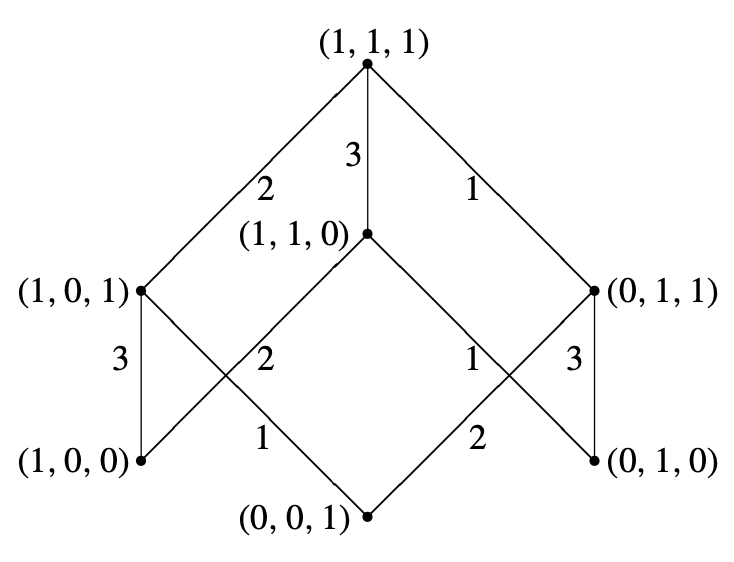
\includegraphics[scale=0.5]{\pref/cubic-example-after-father.png}
    \caption{父亲宣布$p$之后,\Cref{fig:cubic-example} 的变化}
    \label{fig:cubic-example-after-father}
\end{figure}


 在$i$眼中,只有两个可能世界,因此$i$回答“知道”意味着她能够确定只有一个世界;她回答不知道意味着还有两个可能世界.假如现在是第一轮问答.如果所有人都回答了“不知道”,考虑状态$s=(1,0,0,\dots)$.如果真实世界是$s$,那么对于$1$来说,可能世界只有一个了,但是她却说“不知道”,说明真实世界不是$s$.同理,所有那些只有一个$1$的可能世界都会被消掉. 因此,归纳可得,第$k$轮的时候,所有那些只有$k$个$1$的可能世界会被消掉.
 
 如果父亲没有宣布$p$,那么$\mathcal M$是一个超立方体. 无论在任何轮,每一个孩子都会觉得两个可能世界,因此不会有任何可能世界被消掉!因此,从结构上来说,父亲宣布$p$改变了每个孩子对应的$R_i$等价的可能世界,使得一些孩子可以确定自己所处的世界. 
 
这一套方法可以将类似的智力谜题都用算法化的方式得到解答.

\subsection{Aumann结构}

如果我们限制Kripke模型中$R_i$为等价关系,那么认知逻辑还可以有另一种理解方式. 回忆:概率论(或者似然)理解世界的方式基于“事件”. 我们只能感知事件的发生与否,而不能具体知道是哪个样本点. 用事件的方式理解认知,得到的结构被称为\emph{Aumann结构}\index{Aumann结构}.

考虑全集$\Omega$,理解为样本空间. 事件$e\subseteq \Omega$是样本点的集合. 一次观测会落实在一个样本点$\omega$上. 事件$e$发生当且仅当$\omega\in e$. 在Kripke模型中,我们将$i$的知识刻画为了等价关系$R_i$. 在Aumann结构中,对每一个个体$i$,它的知识被刻画为$\Omega$的划分$\mathcal P_i=\{\Omega_j\}$,$\Omega_j$是$\Omega$的子集. $S_j$被称为$i$的\emph{信息集}\index{信息集},可以被理解为$i$能够感知到的最基本的事件. $\mathcal P_i(\omega)$被定义为$\omega$所属于的那个信息集. 

现在我们重新定义算子$K_i:2^\Omega\to 2^\Omega$为$K_i(e):=\{\omega\in\Omega:\mathcal P_i(\omega)\subseteq e\}$. $K_i(e)$定义了“个体$i$知道事件$e$”这一事件. 思想:将所有关于知识的讨论转化为关于事件的讨论. 类似地,可以定义算子$E:2^\Omega\to 2^\Omega$为$E(e)=\bigcap_{i=1}^n K_i(e)$. 定义共同知识算子$C:2^\Omega\to 2^\Omega$为$C(e)=\bigcap_{k=1}^\infty E^k(e)$.

我们再一次看到逻辑和集合的对应,我们总结如\Cref{tab:logic-set-correspondence} 所示.
\begin{table}[ht]
    \centering
    \begin{tabular}{cc}
    \toprule
            Kripke模型&Aumann结构  \\\midrule
            可能世界&样本点\\
            公式&事件\\
            原子命题&基本事件\\
            模态算子&集合-集合映射\\
            $i$的等价关系$R_i$&$i$的划分\\
            逻辑连接词&集合操作\\\bottomrule
    \end{tabular}
    \caption{逻辑与集合的对应关系}
    \label{tab:logic-set-correspondence}
\end{table}

Kripke语义偏好逻辑,Aumann结构偏好(Bayes)概率论,因此用数学来研究知识论就有了两种风格,一种是计算机、逻辑、哲学的风格,另一种是经济学、信息论的风格. 但是,这两种对应关系完全取决于我们对知识的那些基本假设,所以如果这些假设被打破,那么这样的对应关系就不再成立!

下面我们分别用这两种风格来讨论共同知识的意义.


\section{对不一致达成一致}

本部分将用模态逻辑的方式来探讨达成一致与共同知识的关系. 最早由Aumann给出. 我们将要证明,对于有相同决策方式的两个个体来说,他们不可能对采取不同行动这件事具有共同知识. 典型故事:同样的AI之间会发生交易吗?交易发生意味着买家和卖家有不一样的决策(一个买一个卖). 因此,如果两个人按照相同的规则来行事,那么不会有交易发生!

\begin{center}
    players cannot ``agree to disagree''.
\end{center}

首先我们给出模型. 

假想一个含时的系统,有两个玩家1和2. 在任意时刻,每个玩家处于一个状态$s_i$之中.每个玩家分别有一个自己的局部状态空间$S_i$. 整个系统的全局状态是$(s_1,s_2)\in S_1\times S_2=\mathcal G$.时刻是离散的,用非负整数$m$表示,初始时刻是$0$. 系统的一次\emph{运行}指的是函数$r:m\mapsto(s_1,s_2)$. 运行描述了系统每一时刻的全局状态.系统$\mathcal R$指的是$\mathcal G$上所有可能运行的集合.给定$r\in\mathcal R$,$(r,m)$被称为系统$\mathcal R$的一个点.

玩家处于某个状态的时候可以采取某种行动. 为了反映“玩家按照相同的规则行事”这件事,我们规定两个玩家的行动集都是$A$,并且这一集合不依赖于全局或局部的状态. 给定所有人的行动和一个全局状态,我们可以定义系统的\emph{转移函数}为$\tau:A^2\times\mathcal G\to\mathcal G$. 因此,转移函数描述了所有人的行动如何导致系统从一个状态到另一个状态.

如何描述“按照规则行事”?我们用\emph{协议}来描述这种概念. 玩家$i$的协议$P_i$是一个从局部状态$S_i$到行动集$A$的映射,即处于什么状态就做什么事. 两个玩家的联合协议记为$P=(P_1,P_2)$.

一个联合协议要执行起来,还需要初始状态. 初始状态可能的集合记为$\mathcal G_0$. 给定初始状态集$\mathcal G_0$和转移函数$\tau$,我们就可以在系统上执行任何一种协议. 我们把元组$\gamma=(\mathcal G_0,\tau)$称为系统的\emph{上下文}. 

给定上下文$\gamma=(\mathcal G_0,\tau)$和一个联合协议$P$,我们可以讨论$P$产生的所有可能运行. 一个运行$r$与$P$\emph{相容}指的是
    \begin{itemize}
        \item $r(0)\in\mathcal G_0$.
        \item 对任意时刻$m$,如果$r(m)=(s_1,s_2)$,那么$r(m+1)=\tau(P(s_1),P(s_2))(s_1,s_2)$.
    \end{itemize}
换言之,$r$是从跟某个可能的初始状态开始执行协议产生的运行. 一个系统$\mathcal R$表示了上下文$\gamma$和联合协议$P$,指的是所有$r\in\mathcal R$都与$P$相容. 这样的系统我们用记号$\mathcal R^{rep}(P,\gamma)$来表示.


接下来我们引入Kripke模型. Kripke模型的点是系统的点. 设原子命题集$\mathbf P$,它的元素是$perf_i(a)$,表示玩家$i$采取行动$a$. 接下来我们定义赋值函数$V$. 从$\mathbf P$的定义来看,赋值应该只依赖状态,而不依赖时间,所以我们赋值函数实际上需要分两步来定义:
\begin{enumerate}
    \item 定义$V$为从$\mathbf P$到全局状态集合的映射,
    \item 然后再扩展为到系统点集合的映射:$(r,m)\in V(p)\iff r(m)\in V(p)$.
\end{enumerate}
第一步定义如下:状态$s\in V(perf_i(a))$当且仅当在状态$s$玩家$i$采取过行动$a$.

然后我们引入知识算子$K_i$的语义. 同样,我们假设$K_i$对应的是等价关系$\sim_i$. 玩家$i$只能区分自己的局部状态$s_i$,他执行协议时,只有状态,没有时间的概念. 因此我们定义$(r,m)\sim_i (r',m')\iff r(m)_i=r'(m')_i$. 从Aumann结构来说,每一个局部状态$s_i$对应了一个信息集
    \[IS_i(s_i,\mathcal R)=\{(r,m):r\in\mathcal R,r(m)=s_i\}.\]
这样,我们就得到了Kripke点模型$\mathcal M,(r,m)$. $K_i$的语义按照基本认知逻辑定义即可.

接下来,我们引入关于时间的模态算子. 特别地,我们只引入算子$X$,表示“下一时刻”. 它的语义定义为
    \[\mathcal M,(r,m)\vDash X\phi\iff\mathcal M,(r,m+1)\vDash\phi.\]
有了算子$X$,我们可以用公式表达“将要采取行动”:
    \[act_i(a)=\neg perf_i(a)\wedge X perf_i(a).\]

接下来,我们定义关于Kripke模型的\emph{决策函数},用它来在点模型的角度讨论协议的执行. 设Kripke模型的点集为$S$. 玩家$i$的决策函数$D$是从$S$的某些子集到行动集$A$的映射. 我们没有写决策函数的下标,表明两个玩家采取了相同的决策策略. 决策函数描述的是:知道什么样的信息,就采取什么样的行动. 

我们要求协议$P_i$和决策函数$D$是相容的,也就是决策函数在某个信息集上采取的行动恰好是这个协议在该状态要执行的行动:
    \[P_i(s_i)=D(IS_i(s_i,\mathcal R)),\forall s_i\in S_i.\]
反过来说,联合协议$P$在上下文$\gamma$中\emph{实现}了决策函数$D$,如果对所有$i$,$P_i$与$D$在系统$\mathcal R^{rep}(P,\gamma)$中是相容的.

协议和决策函数是两个非常容易混淆的概念,尽管他们有密切联系. 直观来说,协议就是处于什么局部状态采取什么行动,这并不涉及知识的内容. 而决策函数指的是,知道什么信息就采取什么行动,这完全是知识的内容. 在我们的背景下,
    \[\text{知道的信息}=\text{处于的局部状态}.\]
因此二者其实是从不同角度描述同一个概念.

我们对决策函数$D$有一个额外的技术要求,我们要求$D$是\emph{并-一致}的. 具体来说,给定$S$一列互不相交的子集$T_1,\dots,T_k$,每一个都有$D(T_i)=a$,那么我们要求$D(\cup_i T_i)=a$. 考虑一个具体的例子,假设我的决策函数是这样描述的:如果今天下雨,并且今天星期四,那么我会去KFC疯狂星期四;如果今天不下雨,并且今天星期四,那么我会去KFC疯狂星期四. 那么,我的决策还应该有:虽然我不知道今天下不下雨,但是如果今天是星期四,那么我会去KFC疯狂星期四. 可以证明,任何联合协议都可以从某个并-一致的决策函数产生.


至此,模型就已经陈述完了,我们总结一下. 两个玩家处于同一个系统中,每个玩家可能知道不同的东西(局部状态空间不同,信息集不同),但是他们的行动集相同、决策函数相同,决策函数要求是并-一致的,由某个联合协议实现,给定可能的初始状态和系统的转移函数(上下文),系统可以产生一系列可能的运行.

利用这一模型,我们就可以叙述并证明Aumann达成一致定理了. 

\begin{theorem}[Aumann达成一致定理]\index{Aumann达成一致定理}
给定联合协议$P$,上下文$\gamma$,由此产生Kripke框架$\mathcal F$. 设$a,b\in A$是两个不同的行动,如果在上下文$\gamma$中$P$实现了某个并-一致决策函数,那么
\[\mathcal F\vDash\neg C(act_1(a)\wedge act_2(b)).\]
\end{theorem}

如果两个玩家选择了同样的并-一致决策函数,那么他们不可能对“我们采取不同行动”这件事形成共同知识,所以他们不可能对不一致达成一致(agree to disagree).

\begin{proof}
用反证法. 假设某个基于$\mathcal F$的点模型$\mathcal M,(r,m)$使得
    \[\mathcal M,(r,m)\vDash C(act_1(a)\wedge act_2(b)).\]
我们证明$a=b$. 思路如下:共同知识对应了从$(r,m)$出发可到达的状态集$S'$的性质. 从玩家1的视角来看,她在$S'$所关联的信息集上都要采取行动$a$,根据并-一致性,应该有$D(S')=a$. 从玩家2来看同理,因此也应该有$D(S')=b$. 因此$a=b$.

假设$S'$是从$(r,m)$出发,通过关系$\sim_1$或$\sim_2$可到达的点集. 取一个点$(r',m')\in S'$,设$r'(m')_1=s_1'$. 假设$(r'',m'')\sim_1(r',m')$,那么$(r'',m'')\in S'$. 因此,$IS_1(s_1',\mathcal R)\subseteq S'$. 当$s_1'$取遍$S_1$,根据信息集的性质,$S'$是$IS_1(s_1',\mathcal R)$的不交并.

因为$\mathcal M,(r,m)\vDash C(act_1(a))$,所以有$\mathcal M,(r',m')\vDash act_1(a)$. 这一公式意味着$P_1(s_1')=a$. 根据$P$和$D$的关系,这等价于$D(IS_1(s_1',\mathcal R))=a$. 因为这件事对任意$s_1'$都成立,根据$D$的并-一致性,$D(S')=a$. 同理,从玩家2的角度来说$D(S')=b$. 因此$a=b$.
\end{proof}

\begin{remark}
我们的定理是对于确定性的协议证明的. 然而,一个协议可能是非确定的,也就是在一个状态可能会有多种行动的选择,比如选择带有随机性. 这个时候,达成一致定理依然成立,但是我们需要恰当地定义Kripke模型、决策函数以适应非确定性的协议. 当协议具有非确定性时,我们可以用这一模型来理解带有先验知识(分布)、风险或者不确定性下的达成一致定理,只要协议能够对应一个并-一致的决策函数,结论都有效.
\end{remark}


\section{Rubinstein电子邮件博弈}

接下来我们使用Bayes概率论来说明在二人静态博弈中,共同知识对到底实现哪一个Nash均衡非常关键. 此时,知道一件事与否被赋予了不确定性的含义:我确定或不确定某件事发生.

考虑两个玩家和两个可能的收益矩阵:
\begin{table}[ht]
    \centering
\begin{tabular}{c|cc}
&$A$ & $B$ \\
\hline
$A$ & $(0, 0)$ & $(-10, 1)$ \\
$B$ & $(1, -10)$ & $(8, 8)$ \\
\end{tabular}
\qquad
\begin{tabular}{c|cc}
&$A$ & $B$ \\
\hline
$A$ & $(8, 8)$ & $(-10, 1)$ \\
$B$ & $(1, -10)$ & $(0, 0)$ \\
\end{tabular}
\end{table}

在左边的矩阵中,$(B,B)$是唯一的Nash均衡. 在右边的矩阵中有多个Nash均衡:$(A,A)$和$(B,B)$. $(A,A)$给出比$(B,B)$更高的收益,但行动$A$比$B$更有风险.

左边矩阵被选择的概率是$p>1/2$. 玩家1知道真实的矩阵,而玩家2不知道. 如果选择了右边矩阵,玩家1会给玩家2发送一条消息. 如果玩家2收到了消息,她会回复. 如果玩家1收到了回复,她会发送第二条消息来确认她收到了玩家2的回复. 以此类推.  每条消息都以$\epsilon$的概率独立等可能丢失.\footnote{注意:发送电子邮件不是一个行动,而是一个规则.}  

以上传信的过程可以用Bayes博弈的类型来刻画. 具体来说,两个玩家的类型集合为$\Theta_i = \{\theta_i^0, \theta_i^1, \theta_i^2, \dots\}$. $\theta_i^m$表示玩家$i$发了$m$封邮件. $\theta_i^m$有直观的含义. 例如,类型$\theta_1^0$表示真实收益矩阵是左边的.  而类型$\theta_1^1$表示真实收益矩阵是右边的,1发送了一封电子邮件,但2没有收到. 

实际上,$\theta$包含了所有可能的情况:
\begin{itemize}
\item $(\theta_1^0, \theta_2^0)$:真实收益矩阵是左边的. 
\item $(\theta_1^1, \theta_2^0)$:真实收益矩阵是右边的,1发送了一封电子邮件,但2没有收到. 
\item $(\theta_1^1, \theta_2^1)$:真实收益矩阵是右边的,2收到了第一封电子邮件,但1没有收到2的回复. 
\item ……
\end{itemize}

我们可以算出来,当真实矩阵为左边矩阵时,每个类型出现的概率:
\begin{table}[ht]
    \centering
\begin{tabular}{c|cccc}
左& $\theta_2^0$ & $\theta_2^1$ & $\theta_2^2$ & $\cdots$ \\
\hline
$\theta_1^0$ & $p$ & $0$ & $0$ & $\cdots$ \\
$\theta_1^1$ & $0$ & $0$ & $0$ & $\cdots$ \\
$\theta_1^2$ & $0$ & $0$ & $0$ & $\cdots$ \\
$\vdots$ & $\vdots$ & $\vdots$ & $\vdots$ & $\ddots$
\end{tabular}
\end{table}
首先,以概率$p$选择左边的矩阵,而且没有人发送消息. 因此,$(\theta_1^0,\theta_2^0)$的概率是$p$,其他项概率都是$0$.

同样可以算出来,当真实矩阵为右边矩阵时,每个类型出现的概率:
\begin{table}[ht]
    \centering
\begin{tabular}{c|cccc}
右& $\theta_2^0$ & $\theta_2^1$ & $\theta_2^2$ & $\cdots$ \\
\hline
$\theta_1^0$ & $0$ & $0$ & $0$ & $\cdots$ \\
$\theta_1^1$ & $\epsilon(1 - p)$ & $\epsilon(1 - \epsilon)(1 - p)$ & $0$ & $\cdots$ \\
$\theta_1^2$ & $0$ & $\epsilon(1 - \epsilon)^2(1 - p)$ & $\epsilon(1 - \epsilon)^3(1 - p)$ & $\cdots$ \\
$\theta_1^3$ & $0$ & $0$ & $\epsilon(1 - \epsilon)^4(1 - p)$ & $\cdots$ \\
$\vdots$ & $\vdots$ & $\vdots$ & $\vdots$ & $\ddots$
\end{tabular}
\end{table}
首先,以概率$1 - p$选择右边的矩阵,玩家1发送一条消息,它会以概率$\epsilon$丢失. 因此,$(\theta_1^1,\theta_2^0)$的概率是$\epsilon(1 - p)$. 以此类推,可以得到计算. 

对类型$\theta_i^m$,收益矩阵是到第$m$层的共同知识,即$E^m$. 所以对于很大的$m$,收益矩阵是“几乎公共知识”. 信息结构是玩家的共同知识,玩家们进行博弈. 关键问题:这个博弈的BNE是什么?

我们需要弄清楚对每个类型$\theta_i^m$,玩家会做什么. 假设玩家1的类型为$\theta_1^0$. 玩家1知道$(\theta_1^0,\theta_2^0)$是真实的类型,所以左边的矩阵被选择. 据此推理:玩家1选择占优策略$B$.

假设玩家2的类型为$\theta_2^0$. Bayes定理意味着:
\[\Pr(\theta_1^0|\theta_2^0) = \frac{p}{p+\epsilon(1-p)} := \mu_2^0.\] 
此时,左边的矩阵被选择. 
\[\Pr(\theta_1^1|\theta_2^0) = 1 - \mu_2^0.\] 
此时,右边的矩阵被选择. 

选择$B$的期望收益至少是$8\mu_2^0$. 推理如下:类型$\theta_1^0$时肯定选择$B$,因此最坏的情况是$\theta_1^1$选择$B$.

选择$A$的期望收益最多是$-10\mu_2^0 + 8(1 - \mu_2^0)$. 推理如下:类型$\theta_0^1$肯定选择B,因此最好的情况是$\theta_1^1$选择A. 

综合两方面,$B$更好,因为对于所有$\epsilon$,$\mu_2^0 \geq p > \frac{1}{2}$.

假设玩家1的类型为$\theta_1^1$,于是,右边的矩阵被选择. Bayes定理意味着:$\Pr(\theta_2^0|\theta_1^1) = \frac{\epsilon(1-p)}{\epsilon(1-p)+\epsilon(1-\epsilon)(1-p)} = \frac{1}{2-\epsilon} := \mu_1^1$. 另一方面,$\Pr(\theta_2^1|\theta_1^1) = 1 - \mu_1^1$. 

选择$B$的期望收益至少为$0$. 推理如下:类型$\theta_2^0$肯定选择$B$,因此最坏的情况是$\theta_2^1$选择$B$. 

选择$A$的期望收益最多为$-10\mu_1^1 + 8(1 - \mu_1^1)$. 推理如下:类型$\theta_2^0$肯定选择$B$. 最好的情况是$\theta_2^1$选择$A$. 

综合两方面,$B$更好,因为对于所有$\epsilon$,$\mu_1^1 > \frac{1}{2}$. 

逐步迭代上述过程,我们发现,在唯一的BNE中,所有类型都选择$B$. 然而,如果右边的矩阵是共同知识,$(A,A)$是一个严格Nash均衡. 所以,即便收益矩阵是“几乎共同知识”,Nash均衡也不一定是一个可实现的均衡. 

\begin{remark}
    \lhysays{仔细改一改}
    {关于均衡的进一步思考}
\begin{itemize}
    \item 用$Nash(x)$表示“$x$是Nash均衡”,那么$\exists x C(Nash(x))$和$C(\exists x C(Nash(x)))$的含义是否一样?
    \item 如果不引入不确定性,在完全信息下,实现特定的Nash均衡是否还需要共同知识?
    \item 如果玩家不是逻辑全知的,或者说她的推理、计算能力是有限的,那么Nash均衡还是否会达到?是否可接近?
\end{itemize}

\end{remark}


\endgroup

\appendix
\part{附录:预备知识}
\chapter{线性代数基础}\label{chap:linear-algebra}

\section{线性空间}

从动机上说,线性空间试图将$\R^n$或者$\C^n$这样的集合连同他们上面的代数结构抽象出来. 除此之外,函数和无穷数列的集合也是非常重要的对象,比如说$\R$上的连续函数组成的集合$C(\R)$,或者具有“模长”的无穷复数列($\ell^2$空间)\index{$\ell^2$空间}:
\[\ell^2=\left\{(x_1,x_2,\cdots)\in\C^\infty:\sum_{i=1}^\infty x_i^2<\infty\right\}.\]

我们将这些对象的共性抽象出来,得到线性空间的概念. 线性空间都是基于某个域定义的,我们先给出域的定义. 

\begin{definition}[域]\index{域}
一个\textbf{域}是一个集合$F$,其上定义了两种二元运算:加法$+$和乘法$\cdot$,他们都是$F\times F$到$F$的映射,满足下面的公理:
\begin{enumerate}
    \item (结合律)对于任意的$a,b,c\in F$,有$(a+b)+c=a+(b+c)$和$(a\cdot b)\cdot c=a\cdot (b\cdot c)$;
    \item (交换律)对于任意的$a,b\in F$,有$a+b=b+a$和$a\cdot b=b\cdot a$;
    \item(分配律)对于任意的$a,b,c\in F$,有$a\cdot(b+c)=a\cdot b+a\cdot c$. 
    \item (单位元)存在唯一的两个元素$0,1\in F$,使得对于任意的$a\in F$,有$a+0=a$和$a\cdot 1=a$;
    \item (加法逆元)对于任意的$a\in F$,存在唯一$b\in F$,使得$a+b=0$,记$b$作$-a$;
    \item (乘法逆元)对于任意的$a\in F$,如果$a\neq 0$,则存在唯一$b\in F$,使得$a\cdot b=1$,记$b$作$a^{-1}$.
\end{enumerate}
通常将$a\cdot b$写作$ab$,并且乘法的优先级高于加法,即$ab+c=(ab)+c$. 
\end{definition}

域的重要例子包括有理数域$\Q$,实数域$\R$和复数域$\C$,他们都是无限域. 我们将在后面的内容中使用这些域. 接下来,我们定义线性空间. 

\begin{definition}[线性空间,向量空间]\index{线性空间}\index{向量空间}
设$V$是一个集合,$F$是一个域. 如果在$V$上定义了两种运算:加法$+$和数乘$\cdot$,使得$V$满足下面的公理:
\begin{enumerate}
    \item ($V$的结合律)对于任意的$x,y,z\in V$,有$(x+y)+z=x+(y+z)$;
    \item ($V$的交换律)对于任意的$x,y\in V$,有$x+y=y+x$;
    \item (加法零元)存在唯一的元素$0\in V$,使得对于任意的$x\in V$,有$x+0=x$;
    \item (加法逆元)对于任意的$x\in V$,存在唯一$y\in V$,使得$x+y=0$,记$y$作$-x$;
    \item 对于任意的$x\in V$,有$1\cdot x=x$;
    \item 对于任意的$a,b\in F$和$x\in V$,有$(ab)\cdot x=a\cdot (b\cdot x)$;
    \item 对于任意的$a\in F$和$x,y\in V$,有$a\cdot(x+y)=a\cdot x+a\cdot y$;
    \item 对于任意的$a,b\in F$和$x\in V$,有$(a+b)\cdot x=a\cdot x+b\cdot x$. 
\end{enumerate}
则称$V$是一个\textbf{$F$-线性空间},简称\textbf{线性空间},也称\textbf{向量空间}. $V$中的元素被称为\textbf{向量}\index{向量}. 通常将数乘$a\cdot x$写作$ax$,并且乘法的优先级高于加法,即$a\cdot x+y=(a\cdot x)+y$. 
\end{definition}

“线性”一词的含义是指的$ax+by$这种形式的数学对象,线性代数就是研究这种对象的学科. 线性空间的典型例子包括:
\begin{itemize}
    \item $\R^n$和$\C^n$.
    \item $M_{m\times n}(F)$,即所有$m\times n$矩阵组成的集合.
    \item $C(\R)$,即$\R$上的连续函数组成的集合.
    \item $C^k(\R)$,即$\R$上的$k$次连续可微函数组成的集合.
    \item $\ell^2$空间\index{$\ell^2$空间},即所有二次可和的复数序列组成的集合.
\end{itemize}

如同所有其他的代数结构,线性空间也有各式各样构造新的线性空间的方法. 为了看出来线性空间本质的特性,我们有如下引理:

\begin{lemma}\label{lemma:linear-space-subspace}
设$V$是$F$-线性空间,$W$是$V$的一个子集. 则$W$是一个线性空间当且仅当对任意$a,b\in F$和$x,y\in W$,有$ax+by\in W$. 
\end{lemma}
\begin{proof}
    按照定义即可验证. 
\end{proof}

我们给$ax+by$这样的对象一个正式的定义. 

\begin{definition}[线性组合]\index{线性组合}
设$V$是$F$-线性空间,$x_1,\cdots,x_n\in V$,$a_1,\cdots,a_n\in F$,则称$a_1x_1+\cdots+a_nx_n$是$x_1,\cdots,x_n$的一个\textbf{线性组合}. 
\end{definition}

接下来,基于某些特定的线性空间,我们构造各种新的线性空间. 

\begin{definition}[线性子空间]\index{线性子空间}
设$V$是$F$-线性空间,$W$是$V$的一个子集. 如果$W$是一个线性空间,则称$W$是$V$的一个\textbf{线性子空间}. 
\end{definition}

例如,$\Q$是$\R$的一个线性子空间,但$\Z$不是$\R$的一个线性子空间. 再比如,当$k<l$,$C^k(\R)$是$C^l(\R)$的一个线性子空间. 

\begin{definition}[乘积空间]\index{乘积空间}
设$V_1,\cdots,V_n$是$F$-线性空间,则$V_1\times\cdots\times V_n$是一个$F$-线性空间,其中加法和数乘分别定义为
\begin{align*}
    &(x_1,\cdots,x_n)+(y_1,\cdots,y_n)=(x_1+y_1,\cdots,x_n+y_n),\\
    &a(x_1,\cdots,x_n)=(ax_1,\cdots,ax_n).
\end{align*}
\end{definition}

例如,$\R^n$就是$n$个$\R$的乘积空间,$M_{m\times n}(F)$就是$m\times n$个$F$的乘积空间. 

接下来,我们按照\emph{表示论}\index{表示论}的观点,引入基的概念. 线性空间是抽象的数学概念,因此我们需要一些具体的元素去表示这整个空间. 

\begin{definition}[生成集]\index{生成集}
设$V$是$F$-线性空间,$S\subseteq V$,如果$V$中的每一个元素都是$S$的线性组合,则称$S$是$V$的一个\textbf{生成集}. 

更一般地,任意一个$S\subseteq V$,我们可以定义 \textbf{$S$生成的线性子空间}为所有$S$的线性组合的集合,记为$\Span(S)$. 
\end{definition}

我们希望用尽可能少的元素来表示整个线性空间,为此,我们需要把“可表示”这样的概念严格化. 

\begin{definition}[线性相关]\index{线性相关}
设$V$是$F$-线性空间,$S\subseteq V$,如果存在$x_1,\cdots,x_n\in S$,$a_1,\cdots,a_n\in F$,使得$a_1x_1+\cdots+a_nx_n=0$,且至少有一个$a_i\neq 0$,则称$S$是\textbf{线性相关}的,否则称$S$是\textbf{线性无关}的. 
\end{definition}

$S$线性相关意味着$S$中的一些元素可以被另一些元素的线性组合表示出来,因而$S$中有一些冗余. 线性无关意味着$S$中的元素都是必要的,没有冗余. 由此,我们可以给出基的定义. 

\begin{definition}[基]\index{基}
设$V$是$F$-线性空间,$S\subseteq V$,如果$S$是线性无关的,并且$\Span(S)=V$,则称$S$是$V$的一个\textbf{基}. 
\end{definition}

线性空间的一个核心定理是基的存在性定理. 

\begin{theorem}[基的存在性定理]\label{thm:existence-of-basis}
设$V$是$F$-线性空间,则$V$中存在一个基. 
\end{theorem}

要注意,这一定理不是平凡的. 首先,基是线性无关的集合,所以$V$本身通常就不是基. 此外,这一定理要求有一个线性无关的集合$S\subseteq V$,任意向量$x\in V$都可以用$S$中\emph{有限个}元素的线性组合来表示,这样的$S$并不容易找到. 该定理的证明是构造性的,这一构造依赖于选择公理(或者Zorn引理),我们在此略去. 

基的典型例子包括:
\begin{itemize}
    \item $\R^n$的标准基是$\{e_1,\cdots,e_n\}$,其中$e_i$是第$i$个分量为$1$,其余分量为$0$的向量. 
    \item 特别地,$\R$的基就是$\{1\}$,一般地,域$F$作为线性空间的时候,其基就是$\{1\}$. 但如果我们把$\C$看成$\R$的线性空间,那么$\C$的基就是$\{1,i\}$.
    \item $M_{m\times n}(F)$的标准基是$\{E_{ij}:1\leq i\leq m,1\leq j\leq n\}$,其中$E_{ij}$是第$i$行第$j$列为$1$,其余元素为$0$的矩阵. 
\end{itemize}

特别注意,无穷维空间经常违背直觉. 例如,考虑$\ell^2$空间\index{$\ell^2$空间}和向量组$\{e_1,e_2,\cdots\}$,其中$e_i$是第$i$个分量为$1$,其余分量为$0$的实数列. 这个向量组看上去非常像一个基,然而并非如此!比如说,$(1/n)_{n=1}^\infty\in\ell^2$,但是它不能写成有限个$e_i$的线性组合. 实际上,$\ell^2$空间的基一定是不可数的. 

给定一个基,我们可以用基来表示线性空间中的元素,容易证明,这一表示是唯一的. 因此,我们可以把线性空间中的元素看成基的线性组合,因而有了下面的定义. 

\begin{definition}[坐标]\index{坐标}
设$V$是$F$-线性空间,$S$是$V$的一个基,$x\in V$,如果$x=\sum_{v\in S} a_v v$,则称$(a_v)_{v\in S}$是$x$在基$S$下的\textbf{坐标}. 
\end{definition}

例如,$\R^3$的标准基是$\{e_1,e_2,e_3\}$. 任意$x\in\R^3$都可以表示为$x=a_1e_1+a_2e_2+a_3e_3$,其中$a_i$是$x$的第$i$个分量. 因此,我们可以把$x$看成一个三元组$(a_1,a_2,a_3)$,这就是$x$在标准基下的坐标. 这样的讨论也适用于$\R^n$或$\C^n$. 另外,坐标本身的集合也可以被看作是一个线性空间,例如,$\R^3$的坐标集合就是$\R^3$本身. 

线性空间的基可以衡量线性空间的复杂程度,基元素越少,线性空间越简单. 我们可以定义维数来衡量线性空间的复杂程度. 

\begin{definition}[维数]\index{维数}
设$V$是$F$-线性空间,如果$V$的一个基有限,则称$V$是\textbf{有限维}的,否则称$V$是\textbf{无限维}的. 有限维线性空间的基的元素个数称为$V$的\textbf{维数},记为$\dim V$. 
\end{definition}

这一定义隐含的事实是,如果$V$有有限基,那么所有基都是有限的,并且任意两个基的元素个数相同. 我们这里略去证明. 

例如,$\R^n$的维数是$n$,$M_{m\times n}(F)$的维数是$mn$,$C^k(\R)$和$\ell^2$都是无穷维的. 

线性空间可以按照维数递降进行分解,变成越来越简单的线性空间的组合. 这种组合称为\emph{直和}. 

\begin{definition}[和空间与直和]\index{直和}\index{和空间}
设$V$是$F$-线性空间,$U_1,U_2\subseteq V$是$V$的子空间,定义他们的和空间为
\[
    U_1+U_2=\{u_1+u_2:u_1\in U_1,u_2\in U_2\}.
\]
如果$U_1\cap U_2=\{0\}$,换句话说,$U_1$与$U_2$线性无关,则称$U_1+U_2$是\textbf{直和},记为$U_1\oplus U_2$. 如果$V=U_1\oplus U_2$,则称$U_1$和$U_2$是$V$的\textbf{直和分解}\index{直和分解}. 
\end{definition}

例如,$\R^3$可以分解为$\R^3=\R e_1\oplus \R e_2\oplus \R e_3$,其中$\R e_i=\{\alpha e_i:\alpha\in\R\}$是$\R^3$的一维子空间,它们的直和就是$\R^3$. 注意到这个分解将三维线性空间分解成了三个一维线性空间,这不是偶然的,一般地,我们有下面的定理. 

\begin{theorem}[维数定理]\label{thm:dim-thm}\index{维数定理}
设$V$是有限维$F$-线性空间,$V=U_1\oplus U_2$,则
\[
    \dim V=\dim U_1+\dim U_2.
\]
\end{theorem}
\begin{proof}
    设$S_1$是$U_1$的一个基,$S_2$是$U_2$的一个基,那么根据直和的定义,$S_1\cup S_2$是$V$的一个基. 因为$S_1\cup S_2$是线性无关的,所以必然有$S_1\cap S_2=\varnothing$. 又由于$V$中的任意元素都可以写成$S_1\cup S_2$中元素的线性组合,因此
    \[
        \dim V=|S_1\cup S_2|=|S_1|+|S_2|=\dim U_1+\dim U_2.
    \]
\end{proof}
通过直和分解,我们可以把线性空间分成越来越简单的部分. 

\section{线性映射}

接下来我们研究线性空间之间的关系. 并不是所有的关系都是重要的,我们所关心的是保持线性空间代数结构的这种关系,这种关系称为\emph{线性映射}. 

\begin{definition}[线性映射,线性算子,线性函数]\index{线性映射}\index{线性算子}\index{线性函数}\index{线性变换}
设$V$和$W$是$F$-线性空间,如果映射$f:V\to W$满足:
\begin{enumerate}
    \item 对任意$x,y\in V$,$f(x+y)=f(x)+f(y)$;
    \item 对任意$x\in V$和$a\in F$,$f(ax)=af(x)$,
\end{enumerate}
则称$f$是$V$到$W$的一个\textbf{线性映射}. 如果$V=W$,则称$f$是$V$上的一个\textbf{线性算子}或\textbf{线性变换}. 如果$W=F$,则称$f$是$V$上的一个\textbf{线性函数}.
\end{definition}

一个更简洁但也更本质的定义是,线性映射是保持线性组合的映射. 

\begin{example}
一个平凡的例子是\emph{零映射}\index{零映射}:$f:V\to W$,$f(x)=0$,这显然是线性映射,我们通常记为$O$. 另一个平凡的例子是\emph{恒等映射}\index{恒等映射}:$f:V\to V$,$f(x)=x$,这也是线性映射,我们通常记为$\id$.
\end{example}

线性映射有如下基本性质:

\begin{proposition}\label{prop:linear-map-basic}
设$f:V\to W$是域$F$上的线性映射,那么
\begin{enumerate}
    \item $f(0)=0$;
    \item $f(-x)=-f(x)$;
    \item $f(\sum_{i=1}^n a_ix_i)=\sum_{i=1}^n a_if(x_i)$;
    \item 如果$g:W\to Z$是线性映射,则$g\circ f:V\to Z$也是线性映射;
    \item 如果$g:V\to W$是线性映射,$a,b\in F$,则$af+bg:x\mapsto af(x)+bg(x)$也是线性映射;
    也是线性映射;
    \item 如果$g:V\to W$是线性映射,$h:W\to Z$是线性映射,$k:Z\to V$是线性映射,则$h\circ(f+g)=h\circ f+h\circ g$,$(f+g)\circ k = f\circ k+g\circ k$;
    \item 如果$f$是双射,则$f^{-1}$也是线性映射. 
\end{enumerate}
\end{proposition}
\begin{proof}
    按照定义验证即可. 
\end{proof}

为了简化记号,我们会将线性映射$f$的作用$f(x)¥$简记为$fx$,线性映射的复合$g\circ f$简记为$gf$,同一线性映射$f$的$n$次复合简记为$f^n$. 对于多项式函数$G(x)=a_0+a_1x+\cdots+a_nx^n$,我们可以定义一个新的线性映射$G(f)=a_0\id+a_1f+\cdots+a_nf^n$. 

线性映射可以被看成一种滤镜,它可以将原始的空间进行变形,变成一个新的空间. 比如说,海上的月亮,就是将三维空间的太阳与空间映到了海面上. 而线性算子则是一种特殊的线性映射,它将原始空间变形成自身. 如果我们把线性空间看成一块橡皮泥,那么线性算子可以被看成某种拉伸,橡皮泥这个整体没有变多或者变少,但是橡皮泥的形状发生了改变. 

下面我们考虑两个线性映射的例子. 

\begin{example}[微分算子]\index{微分算子}
考虑$C^\infty(\R)$,即任意次可微的实函数空间. 求导$\d/\d x:C^\infty(\R)\to C^\infty(\R)$被称为\textbf{微分算子}. 容易验证,$\d/\d x$是线性算子. 
\end{example}

\begin{example}[投影变换]\index{投影变换}
这个例子实际上是海上升明月的一般化. 考虑$\R^n$,设$m\leq n$. 映射
\[\pi_m:(x_1,\dots,x_n)\mapsto (x_1,\dots,x_m,0,\dots,0)\]
称为$\R^n$的\textbf{投影变换}. 容易验证,$\pi_m$是线性算子. 此外,实际上,$\pi_m$也可以被看作是$\R^n$到$\R^m$的线性映射,将$(x_1,\dots,x_m,0,\dots,0)$后面的$0$都丢掉,这就是一个$\R^m$的元素. 
\end{example}

从投影变换的例子中,我们可以体会到线性空间的微妙之处:不同的线性空间可能有着完全相同的本质. 由$(x_1,\dots,x_m,0,\dots,0)$形成的空间实际上就是$\R^m$,只是我们用了$\R^n$的元素来表示它. 这里引申出来了代数中两个重要的概念:\emph{同态}与\emph{同构}. 

\begin{definition}[同态与同构]\index{同态}\index{同构}
设$V$和$W$是$F$-线性空间,如果映射$f:V\to W$满足:
\begin{enumerate}
    \item 对任意$x,y\in V$,$f(x+y)=f(x)+f(y)$;
    \item 对任意$x\in V$和$a\in F$,$f(ax)=af(x)$,
\end{enumerate}
则称$f$是$V$到$W$的一个\textbf{同态}. 如果$f$是一个满射,那么称$f$是一个\textbf{满同态};如果$f$还是一个单射,那么称$f$是一个\textbf{同构}. 
\end{definition}

线性空间之间的同态实际上就是线性空间之间的线性映射,所以同态是平凡的概念. 同态这个词表明了两个线性空间的相似性,一个空间丢掉一些东西之后就可以被看成另一个空间的子空间. 而满同态则是说,丢掉一些东西之后,这个空间就是另一个空间. 比如说,如果$m<n$,丢掉$\R^n$中元素的后面$n-m$个分量,就得到了$\R^m$,这就是一个满同态. 同构则是说,这两个线性空间就是一样的,没有谁比谁更复杂,比如说,$\R^n$和$\R^m$就是同构的,只要$n=m$. 

刚刚讨论的$\R^m$与$\R^n$的同构是具有一般性的,这就是有限维线性空间的同构定理:

\begin{theorem}[有限维线性空间的同构定理]\label{thm:finite-dim-linear-space-isomorphism}\index{同构定理}
设$V$和$W$是有限维$F$-线性空间,则$V$与$W$同构当且仅当$\dim V=\dim W$. 
\end{theorem}
这一定理充分说明了,有限维线性空间中维数的意义:维数刻画了线性空间. 
\begin{proof}
    这一证明的思路是典型的:先定义一个(与基相关的)基本映射,然后进行扩张. 
    
    $\impliedby$:如果$\dim V=\dim W=n$,那么两个线性空间的基的元素个数是一样的,我们可以将它们一一对应起来. 比方说$V$的基是$\{v_1,\dots,v_n\}$,$W$的基是$\{w_1,\dots,w_n\}$,那么我们可以定义两个基之间的映射$f$,使得$f(v_i)=w_i$. 
    
    我们可以将$f$扩张成一个线性映射. 比如说,对于任意的$x\in V$,它用基表示就是$\sum_{i=1}^n a_iv_i$. 我们可以定义
    \[f(x)=f\left(\sum_{i=1}^n a_iv_i\right)=\sum_{i=1}^n a_if(v_i)=\sum_{i=1}^n a_iw_i.\]

    接下来验证$f$是$V$到$W$同构. 首先,按照定义就可以验证这是一个线性映射. 其次,因为$a_i$是任意的,所以这显然也是一个满射. 最后,如果有两个不同的$x,y$对应相同的$f(x)=f(y)$,那么$f(x)$和$f(y)$的坐标是一样的,所以$x$和$y$的坐标也是一样的,所以$x=y$,所以$f$也是一个单射. 

    $\implies$:设两个线性空间由映射$f:V\to W$给出同构. 假设$V$的基是$\{v_1,\dots,v_n\}$,我们证明$W$的基就是$\{f(v_1),\dots,f(v_n)\}$. 
    
    首先,因为$f$是满射,而$v_i$生成了整个$V$,所以$f(v_i)$生成了整个$W$. 
    
    再说明$f(v_i)$线性无关. 假设$\sum_{i=1}^n a_if(v_i)=0$,那么$f(\sum_{i=1}^n a_iv_i)=0$,由于$f$是单射,所以$\sum_{i=1}^n a_iv_i=0$,由于$v_i$线性无关,所以$a_i=0$,所以$f(v_i)$线性无关. 
    
    以上两点证明了$W$的基是$\{f(v_1),\dots,f(v_n)\}$,所以$\dim V=\dim W$. 
\end{proof}

此外,同构还有一个重要性质:
\begin{proposition}\label{prop:isomorphism-composition}
假设$f:V\to W$和$g:W\to U$是两个线性映射,如果$f$和$g$都是同构,那么$g\circ f$也是同构. 
\end{proposition}
\begin{proof}
    根据定义即可证明.     
\end{proof}



接下来我们进一步研究线性映射所带来的结构. 我们刚刚说过,同态就是说把一些东西丢掉,剩下的东西可以被看成另一个空间的子空间. 丢掉的东西是和剩下的东西,就是线性映射的\emph{核}与\emph{像}. 

\begin{definition}[核与像]\label{def:kernel-image}\index{核}\index{像}
设$V$和$W$是$F$-线性空间,$f:V\to W$是一个线性映射. $f$的\textbf{核}定义为$\ker f=\{x\in V:f(x)=0\}$,$f$的\textbf{像}定义为$\im f=\{f(x):x\in V\}$. 
\end{definition}

“把一些东西丢掉”这一表述可以精确地由以下定理给出:

\begin{theorem}\label{thm:kernel-image-property}
设$V$和$W$是$F$-线性空间,$f:V\to W$是一个线性映射,则$\ker f$是$V$的线性子空间,$\im f$是$W$的线性子空间. 另外,
\[\dim V=\dim\ker f+\dim\im f.\]
\end{theorem}
直观来说,这一定理表明,线性映射$f$把$V$抹掉了子空间$\ker f$,最终得到了空间$\im f$. 
\begin{proof}
这一证明类似于\Cref{thm:finite-dim-linear-space-isomorphism} 的证明,这里只给出思路,细节留给读者. 首先选出$\ker f$的基$v_1,\dots,v_k$,然后添加向量$u_1,\dots,u_l$扩充成$V$的基,然后证明$f(u_1),\dots,f(u_l)$是$\im f$的基. 
\end{proof}

一个直接但重要的推论是:
\begin{corollary}\label{cor:kernel-image-isomorphism}
设$V$和$W$是$F$-线性空间,$f:V\to W$是一个线性映射. 那么以下性质成立:
\begin{enumerate}
    \item $\dim \im f\leq \dim V$,等号成立当且仅当$\ker f=\{0\}$;
    \item $f$是单射当且仅当$\ker f=\{0\}$;
    \item $f$是满射当且仅当$\dim \im f=\dim W$;
    \item $f$是同构当且仅当$\ker f=\{0\}$且$\dim \im f=\dim W$. 
\end{enumerate}
\end{corollary}
这一推论给了我们判断一个线性映射是否是单射、满射或者同构的方法. 

最后,我们引入线性映射的秩的概念:
\begin{definition}[线性映射的秩]\index{秩}
设$V$和$W$是$F$-线性空间,$f:V\to W$是一个线性映射. $f$的\textbf{秩}定义为$\rank f=\dim\im f$. 
\end{definition}

换言之,线性映射的秩就是它的像的维数. 秩越高的线性映射说明它把空间“压缩”得越少,丢掉的东西越少. 例如,$\R^n$的投影变换$\pi_m$的秩为$m$,说明它丢掉的东西只有$n-m$维,也就是后面的$n-m$个坐标. 

\Cref{cor:kernel-image-isomorphism} 给出了复合线性映射秩的性质:
\begin{corollary}\label{cor:rank-composition}
设$V$、$W$和$U$是$F$-线性空间,$f:V\to W$和$g:W\to U$是两个线性映射,则$\rank (g\circ f)\leq \rank f$,等号成立当且仅当$\im f\cap \ker g=\{0\}$. 特别地,如果$f,g$都是满射,那么等号成立当且仅当$g$是同构. 此外,$\rank (g\circ f)\leq \rank g$,如果$f$是满射,那么等号成立. 
\end{corollary}
\begin{proof}
    根据\Cref{cor:kernel-image-isomorphism},我们有$\rank (g\circ f)=\dim\im (g\circ f)\leq \dim \im f=\rank f$. 等号成立当且仅当在空间$\im f$中$g$的核是$\{0\}$,换言之,$\im f\cap \ker g=\{0\}$. 特别地,如果$f$是满射,那么这一条件变为$\ker g=\{0\}$,如果$g$也是满射,那么$g$是同构. 
    
    此外,因为$\im f\subseteq W$,所以$\im (g\circ f)\subseteq \im g$,因此$\rank (g\circ f)=\dim\im (g\circ f)\leq \dim \im g=\rank g$. 如果$f$是满射,那么$\im f=W$,所以$\im (g\circ f)=\im g$,因此等号成立. 
\end{proof}

这一推论有非常直观的含义:线性映射是同态,因此会丢东西,所以复合映射会丢更多的东西. 

\section{矩阵}\label{sec:matrix}

我们已经用用基与坐标表示了线性空间,接下来,我们引入\emph{矩阵}的概念来表示线性映射,我们这一节考虑的线性空间都是有限维的. 考虑一个线性映射$f:V\to W$,如果$V$的基是$\{v_1,\dots,v_n\}$,$W$的基是$\{w_1,\dots,w_m\}$,那么$f(v_i)$可以用$w_1,\dots,w_m$的线性组合表示出来,即
\[f(v_i)=a_{1i}w_1+\cdots+a_{mi}w_m.\]
我们把这些系数$a_{ji}$排成如下形状
\[A=\begin{pmatrix}
a_{11}&a_{12}&\cdots&a_{1n}\\
a_{21}&a_{22}&\cdots&a_{2n}\\
\vdots&\vdots&\ddots&\vdots\\
a_{m1}&a_{m2}&\cdots&a_{mn}
\end{pmatrix}.\]

此时$A$被称为\emph{矩阵}\index{矩阵}. $m=n$的矩阵被称为\emph{方阵}. $A_i=(a_{i1},\dots,a_{in})$被称为矩阵$A$的第$i$行,$A^j=\begin{pmatrix}a_{1j}\\\vdots\\a_{mj}\end{pmatrix}$被称为矩阵$A$的第$j$列. 他们分别被叫做\emph{行向量}与\emph{列向量}. 第$i$行第$j$列的元素,也就是$a_{ij}$,记为$A_{ij}$. 为了节约空间,列向量通常被写成转置的形式,即$(a_{1j},\dots,a_{mj})^\t$. 注意,坐标向量都被视作列向量. 

假设在基$v_i$下$x\in V$的坐标是$X=(x_1,\dots,x_n)^\t$. 我们现在来计算$f(x)$在基$w_i$下的坐标$Y=(y_1,\dots,y_m)^\t$. 因为$x=x_1v_1+\cdots+x_nv_n$,所以
\begin{align*}
    f(x)&=f(x_1v_1+\cdots+x_nv_n)\\
    &=x_1f(v_1)+\cdots+x_nf(v_n)\\
    &=x_1(a_{11}w_1+\cdots+a_{m1}w_m)+\cdots+x_n(a_{1n}w_1+\cdots+a_{mn}w_m)\\
    &=(a_{11}x_1+\cdots+a_{1n}x_n)w_1+\cdots+(a_{m1}x_1+\cdots+a_{mn}x_n)w_m.
\end{align*}

因此,$f(x)$在基$w_i$下的坐标是$(a_{11}x_1+\cdots+a_{1n}x_n,\dots,a_{m1}x_1+\cdots+a_{mn}x_n)^\t$,$y_i=a_{i1}x_1+\cdots+a_{in}x_n$. 我们将这一计算结果写作
\[Y=AX.\]
这就是矩阵与向量的乘法.

通过矩阵,线性映射作用在向量上的结果可以被具体算出来. 从这个意义上说,矩阵表示了线性映射. 这一观点可以用下图来表示:
\[\begin{tikzcd}
    x\arrow[r,mapsto,"f"]\arrow[d,mapsto]&f(x)\arrow[d,mapsto]\\
    X\arrow[r,mapsto,"A"]&Y
    \end{tikzcd}\] 

反之,给定一个域$F$上的$m\times n$矩阵$A$,我们可以定义一个线性映射$f_A:F^n\to F^m$:对$X\in F^n$,$f_A(X)=AX$. $f_A$被称为$A$\emph{诱导的线性映射}. 所以,矩阵本身也可以看成是一个线性映射,不仅仅只是线性映射的表示. 

我们看一个平凡的例子. 考虑零映射$O:x\mapsto 0$. 不管在什么基下,$O$的矩阵都是全零矩阵,我们称为\emph{零矩阵},依然使用符号$O$表示. 反过来,如果一个线性映射的矩阵是零矩阵,那么这个线性映射也是零映射. 

我们再看一个的例子,这个例子说明利用矩阵如何给出不同基之下的坐标变换公式. 设$V$是一个$n$维线性空间,$f:V\to V$是一个线性算子. $V$的一组基是$\{v_1,\dots,v_n\}$,另一组基是$\{v_1',\dots,v_n'\}$. 定义一个$V$的自同构满足$f(v_i)=v_i'$. 假设$f$在基$\{v_i\}$下的矩阵是$A$,这被称为基$\{v_i\}$到基$\{v_i'\}$的\emph{过渡矩阵}\index{过渡矩阵}.

考虑一个点$x\in V$,它在基$\{v_i\}$下的坐标是$X=(x_1,\dots,x_n)^\t$,在基$\{v_i'\}$下的坐标是$X'=(x_1',\dots,x_n')^\t$. 我们来计算$x$在基$\{v_i'\}$下的坐标. 因为$f(x)=f(x_1v_1+\cdots+x_nv_n)=x_1f(v_1)+\cdots+x_nf(v_n)$,而
\[f(v_i)=v_i'=\sum_{j=1}^n a_{ji}v_j,\]
所以
\begin{gather*}
f(x)=\sum_{i=1}^n x_i\sum_{j=1}^n a_{ji}v_j=\sum_{j=1}^n\left(\sum_{i=1}^n a_{ji}x_i\right)v_j\implies\\
 x=\sum_{j=1}^n\left(\sum_{i=1}^n a_{ji}x_i\right)f^{-1}(v_j)=\sum_{j=1}^n\left(\sum_{i=1}^n a_{ji}x_i\right)v_j'.
\end{gather*}
因此,$X=AX'$.


线性映射相关的概念就可以被迁移到矩阵中来. 

首先我们考虑映射的线性组合. 设$V$是$F$-线性空间,$f:V\to W$和$g:V\to W$是两个线性映射,$\lambda,\mu\in F$,那么$\lambda f+\mu g$也是一个线性映射. 如果$V$的基是$\{v_1,\dots,v_n\}$,$W$的基是$\{w_1,\dots,w_m\}$. 假设在这些基下,$f$和$g$的矩阵分别是$A$和$B$,那么$\lambda f+\mu g$的矩阵可以很自然地记作$\lambda A+\mu B$. 容易验证,$\lambda A+\mu B$的第$i$行第$j$列的元素是$\lambda a_{ij}+\mu b_{ij}$. 用这样的办法,我们就定义了矩阵的\emph{数乘}和\emph{加法}. 


然后再考虑映射的复合. 设$V$是$F$-线性空间,$f:V\to W$和$g:W\to U$是两个线性映射. 如果$V$的基是$\{v_1,\dots,v_n\}$,$W$的基是$\{w_1,\dots,w_m\}$,$U$的基是$\{u_1,\dots,u_l\}$. 假设在这些基下,$g$和$f$的矩阵分别是$A$和$B$,那么复合$gf$的矩阵可以很自然地记作$AB$. 我们来计算$AB$的第$i$行第$j$列的元素. 因为$gf(v_i)=g(f(v_i))$,所以
\begin{align*}
    gf(v_i)&=g(f(v_i))\\
    &=g(a_{1i}w_1+\cdots+a_{mi}w_m)\\
    &=a_{1i}g(w_1)+\cdots+a_{mi}g(w_m)\\
    &=a_{1i}(b_{11}u_1+\cdots+b_{l1}u_l)+\cdots+a_{mi}(b_{1m}u_1+\cdots+b_{lm}u_l)\\
    &=(a_{1i}b_{11}+\cdots+a_{mi}b_{1m})u_1+\cdots+(a_{1i}b_{l1}+\cdots+a_{mi}b_{lm})u_l.
\end{align*}
因此,$AB$的第$i$行第$j$列的元素是$a_{1i}b_{j1}+\cdots+a_{mi}b_{jm}$. 这就是矩阵乘法的定义. 当有多个相同矩阵相乘时,我们可以写成幂的形式. 比如,$A^2=AA$,$A^3=AAA$等等. 

接下来,我们考虑同构对应的矩阵. 最简单的同构是恒等映射$\id:V\to V$,它的矩阵是\emph{单位矩阵}\index{单位矩阵} $I_n$. 容易看出,无论在什么基下,$I_n$都等于
\[\begin{pmatrix}
1&0&\cdots&0\\
0&1&\cdots&0\\
\vdots&\vdots&\ddots&\vdots\\
0&0&\cdots&1
\end{pmatrix}.\]

有了单位矩阵,类似算子的多项式,给定多项式$G(x)=a_0+a_1x+\cdots+a_nx^n$,我们可以定义矩阵$G(A)=a_0I_n+a_1A+\cdots+a_nA^n$. 

在更一般的情况下,考虑$V$和$W$是$n$维的$F$-线性空间,基分别是$\{v_1,\dots,v_n\}$和$\{w_1,\dots,w_n\}$. 如果线性映射$f:V\to W$将$v_i$映到$\lambda_i w_i$,那么$f$的矩阵就是
\[\begin{pmatrix}
\lambda_1&0&\cdots&0\\
0&\lambda_2&\cdots&0\\
\vdots&\vdots&\ddots&\vdots\\
0&0&\cdots&\lambda_n
\end{pmatrix}.\]
我们将这样的矩阵称为\emph{对角矩阵}\index{对角矩阵}. 

对于一般的同构映射$f:V\to W$,它有一个同构逆映射$f^{-1}:W\to V$. 假设$V$的基是$\{v_1,\dots,v_n\}$,$W$的基是$\{w_1,\dots,w_n\}$,那么$f$和$f^{-1}$的矩阵分别是$A$和$B$. 我们来计算$AB$和$BA$. 因为$f^{-1}f=\id$,所以$AB=I_n$. 同理,$BA=I_n$. $B$可以被看成$A$的逆元,我们记作$B=A^{-1}$. 这就是矩阵的\emph{逆}的定义. 

接下来,我们引入矩阵\emph{转置}的概念. 

\begin{definition}[矩阵转置]\index{转置}
    设$A=(a_{ij})$是一个$m\times n$矩阵,我们定义$A$的\textbf{转置}\index{转置}为一个$n\times m$矩阵$A^\t=(a_{ji})$.
\end{definition}

实矩阵的转置在线性映射中对应的是对偶空间的对偶映射,这里我们不展开讨论了. 

对于满足$A^\t=A$的矩阵,我们称之为\textbf{对称矩阵}\index{对称矩阵}. 对于满足$A^\t=-A$的矩阵,我们称之为\textbf{反对称矩阵}\index{反对称矩阵}. 

现在,矩阵作为一个代数结构所需要的要素都已经给出了. 我们来看看矩阵的一些基本性质. 这些性质大多是从线性映射继承过来的(\Cref{prop:linear-map-basic}),我们在此略去证明. 

\begin{proposition}\label{prop:mat-basic}
    设$A,B,C$都是域$F$上的$n$阶方阵,$\lambda,\mu\in F$,那么
    \begin{enumerate}
        \item $(\lambda A+\mu B)C=\lambda AC+\mu BC$;
        \item $A(\lambda B+\mu C)=\lambda AB+\mu AC$;
        \item $(AB)C=A(BC)$;
        \item $A(B+C)=AB+AC$;
        \item $(A+B)C=AC+BC$;
        \item $AI_n=I_nA=A$;
        \item $AO=OA=O$;
        \item $A(-B)=(-A)B=A(-B)=-(AB)$;
        \item $(AB)^{-1}=B^{-1}A^{-1}$;
        \item $(A^{-1})^{-1}=A$;
        \item $(\lambda A)^{-1}=\lambda^{-1}A^{-1}$;
        \item $(A^\t )^{-1}=(A^{-1})^\t $;
        \item $(A^\t )^\t =A$;
        \item $(A+B)^\t =A^\t +B^\t $;
        \item $(AB)^\t =B^\t A^\t $;
        \item $(\lambda A)^\t =\lambda A^\t $;
        \item $(A^{-1})^\t =(A^\t )^{-1}$;
        \item $(A^\t )^{-1}=(A^{-1})^\t $.
    \end{enumerate}
\end{proposition}

回顾前面关于矩阵的表示论观点,从线性映射$f$得到矩阵$A$需要基于给定的基. 一个自然的问题是,如果我们换了基,那么矩阵$A$会怎么变化?下面我们来具体计算. 

设$f:V\to V$是一个线性算子,$V$的两个基分别是$\{v_1,\dots,v_n\}$和$\{v_1',\dots,v_n'\}$. 假设在这两个基下,$f$的矩阵分别是$A=(a_{ij})$和$A'=(a_{ij}')$. 我们来计算$A'$和$A$的关系. 

假设$g$是一个自同构,使得$g(v_i)=v_i'$,在$\{v_1,\dots,v_n\}$下对应的矩阵是$B$. 我们下面证明$A'=B^{-1}AB$,注意到
\[fg(v_i)=f(g(v_i))=f(v_i')=\sum_{j}a_{ji}'v_j'=\sum_{j}a_{ji}'g(v_j),\]
因为$g$可逆,所以
\[g^{-1}fg(v_i)=\sum_{j}a_{ji}'v_j.\]
左边是$B^{-1}AB$,而右边对应的就是$A'$. 所以我们证明了

\begin{theorem}\label{thm:base-change}
    设$V$是$F$-线性空间,$f:V\to V$是一个线性算子,$\{v_1,\dots,v_n\}$和$\{w_1,\dots,w_n\}$是$V$的两个基. 假设$A$和$A'$分别是$f$在这两个基下的矩阵,$B$是从$\{v_1,\dots,v_n\}$到$\{w_1,\dots,w_n\}$的过渡矩阵,那么$A'=B^{-1}AB$. 
\end{theorem}

矩阵$A$和$A'$通过可逆矩阵$B$联系了起来:$A'=B^{-1}AB$,行如这样的矩阵关系被称为\emph{相似}\index{相似},记作$A\sim A'$. 容易验证,相似是一个等价关系,也就是说:
\begin{itemize}
    \item $A\sim A$;
    \item 如果$A\sim A'$,那么$A'\sim A$;
    \item 如果$A\sim A'$,$A'\sim A''$,那么$A\sim A''$.
\end{itemize}

根据上面的讨论,矩阵的相似关系对应了基的变换:如果我们把$V$的基换成$V$的另一个基,那么线性算子$f$的矩阵也会变成相似的另一个矩阵. 

最后,我们讨论矩阵的秩. 同样,这一定义来自线性映射的🈯秩

\begin{definition}[矩阵的秩,行空间,列空间]\index{秩}\index{行空间}\index{列空间}
设$A$是一个$m\times n$矩阵,$f_A:F^n\to F^m$是它诱导的线性映射.
\begin{itemize}
    \item 定义$A$的\textbf{秩}\index{秩}为$f_A$的秩,记为$\rank A$.
    \item $A$的$m$个行向量生成了一个线性空间,称为矩阵$A$的\textbf{行空间}\index{行空间};类似地,所有的列向量生成了一个线性空间,称为矩阵$A$的\textbf{列空间}\index{列空间}.
    \item 行空间的维数称为矩阵$A$的\textbf{行秩}\index{行秩},列空间的维数称为矩阵$A$的\textbf{列秩}\index{列秩}.
    \item 如果行秩等于$m$,即行空间的一组基就是所有行向量,那么我们称$A$是\textbf{行满秩}\index{行满秩}的;如果列秩等于$n$,即列空间的一组基就是所有列向量,那么我们称$A$是\textbf{列满秩}\index{列满秩}的.
    \item  对于方阵来说,如果它同时是行满秩的和列满秩的,那么我们称它是\textbf{满秩}\index{满秩}的. 
\end{itemize}
\end{definition}

矩阵的秩最核心的定理是:

\begin{theorem}\label{thm:rank}
    设$A$是一个$m\times n$矩阵,$A$的行秩、列秩与秩都相等. 
\end{theorem}

这一定理的证明通常涉及到矩阵的初等行变换,也可以用对偶空间理论的证明,我们这里就不给出了. 

从线性映射复合的秩关系(\Cref{cor:rank-composition}),我们直接得到了矩阵乘法秩的性质:

\begin{proposition}\label{prop:rank-multiplication}
    设$A$是一个$m\times n$矩阵,$B$是一个$n\times p$矩阵,那么
    \[\rank(AB)\leq \min\{\rank A,\rank B\}.\]
如果$A$和$B$都是方阵,那么当$A$可逆时,$\rank(AB)=\rank B$;当$B$可逆时,$\rank(AB)=\rank A$.
\end{proposition}

\section{双线性型与二次型}

本节考虑线性函数的一种推广,即\emph{双线性函数}. 它是两个变量的函数,而且每个变量都是线性的. 这种函数在几何上有很多应用,比如内积. 我们先来给出它的定义. 

\begin{definition}[双线性型]\label{def:bilinear-form}\index{双线性型}
    设$V$是一个$F$-线性空间,如果$V$上有一个映射$f:V\times V\to F$,满足
    \begin{enumerate}
        \item 对于任意的$v\in V$,$f(v,\cdot):V\to F$是一个线性映射;
        \item 对于任意的$w\in V$,$f(\cdot,w):V\to F$是一个线性映射. 
    \end{enumerate}
    那么称$f$是$V$上的一个\textbf{双线性型}. 
\end{definition}

类似线性映射,我们的首要任务是表示一个双线性型. 实际上,双线性型也可以用矩阵来表示. 选定一组$V$的基$\{v_1,\dots,v_n\}$,任意给定两个向量$x=\sum_{i=1}^n x_iv_i$和$y=\sum_{i=1}^n y_iv_i$,我们有
\begin{align*}
    f(x,y)&=f\left(\sum_{i=1}^n x_iv_i,\sum_{j=1}^n y_jv_j\right)\\
    &=\sum_{i=1}^n\sum_{j=1}^n x_iy_jf(v_i,v_j).
\end{align*}

如果我们知道了$f(v_i,v_j)$,那么$f(x,y)$就完全可以用$x,y$的坐标表示出来. 这就是说,我们可以用矩阵来表示双线性型. 定义$A_{ij}=f(v_i,v_j)$,我们将矩阵$A=(A_{ij})$称为$f$在基$\{v_1,\dots,v_n\}$下的\emph{矩阵}. 假设$x,y$的坐标是$X,Y$,那么我们有
\[
    f(x,y)=X^\t AY.
\]

反过来,如果给定了一个$n$阶方阵$A$,那么我们可以定义一个双线性型$f_A$,使得$f_A(v_i,v_j)=a_{ij}$,这样的双线性型称为\emph{由矩阵$A$诱导的双线性型}. 于是,双线性型就和矩阵一一对应了. 

类似线性映射,双线性映射关心的一个重要问题是基变换. 设$A$是一个双线性型$f$在基$\{v_1,\dots,v_n\}$下的矩阵,而$A'$是基$\{v_1',\dots,v_n'\}$下的矩阵,假设$\{v_i\}$到$\{v_i'\}$的过渡矩阵是$P$. 现在任取$x,y\in V$,他们在基$\{v_i\}$下的坐标分别是$X,Y$,在基$\{v_i'\}$下的坐标分别是$X',Y'$,那么我们有
\[
    f(x,y)=X^\t AY=X'^\t A'Y'.
\]
根据坐标的基变换公式,$X=PX'$,$Y=PY'$,所以
\[
    X^\t AY=(AX')^\t P(AY')=X'^\t (A^\t P A)Y'.
\]
由于$x,y$是任意的,$X,Y$也是任意的,联立上面两式,$A'=A^\t P A$,这就是基变换公式. 对应到矩阵中,这被称为\emph{合同变换}. 

\begin{definition}[合同矩阵]\label{def:congruent-matrix}\index{合同矩阵}
    设$A,B$都是$n$阶方阵,如果存在一个可逆方阵$P$,使得$B=P^\t A P$,那么称$A$和$B$是\textbf{合同的}. 
\end{definition}

容易验证,合同关系是一个等价关系,这与相似关系是类似的. 根据\Cref{prop:rank-multiplication},可逆矩阵相乘不改变矩阵的秩,所以合同矩阵的秩是相同的. 于是,双线性型的任意矩阵表示都有相同的秩,我们因此可以定义双线性型的秩:

\begin{definition}[双线性型的秩]\label{def:bilinear-form-rank}\index{秩}
    设$f$是$V$上的一个双线性型,如果$f$在某个基下的矩阵的秩是$r$,那么称$f$的\textbf{秩}是$r$.
\end{definition}

接下来,我们考虑一种特殊的双线性型:对称双线性型,即$f(x,y)=f(y,x)$对任意$x,y\in V$成立. 注意到,对称双线性型对应的矩阵是对称矩阵. 我们现在令$x=y$,定义$q(x)=f(x,x)$,那么$q$是一个实值函数,这样的函数便是\emph{二次型}. 

\begin{definition}[二次型]\label{def:quadratic-form}\index{二次型}
    设$V$是数域$F$上的线性空间,$f$是$V$上的一个对称双线性型,那么定义$q:V\to F$为$q(x)=f(x,x)$,称$q$是$f$诱导的\textbf{二次型}. 
\end{definition}

自然,秩的概念也可以被迁移到二次型上:
\begin{definition}[二次型的秩]\label{def:quadratic-form-rank}\index{秩}
设$q$是$V$上的一个二次型,如果定义$q$的\textbf{秩}为诱导它的双线性型$f$的秩. 
\end{definition}

实际上,二次型本身也可以算出双线性型:设$q$是二次型,那么我们可以定义
\[f(x,y)=\frac{1}{2}(q(x+y)-q(x)-q(y)).\]
容易验证,$f$是一个对称双线性型. 于是,二次型和对称双线性型是一一对应的. 

自然,二次型也可以用坐标表示. 选定一组基,假设二次型$q$对应的对称双线性型是$f$,那么$q$在这组基下的矩阵就是$f$在这组基下的矩阵. 这样,二次型就和对称矩阵一一对应了. 如果再给定$x\in V$的坐标$X$,那么$q(x)=X^\t AX$. 如果把它展开写,就是
\[
    q(x)=\sum_{i=1}^n\sum_{j=1}^n a_{ij}x_ix_j.
\]
这是一个关于$x_i$的二次函数. 通常来说,我们希望化简这一表示,如果能写成$\sum_{i=1}^n a_{ii}x_i^2$的形式,那么计算都会变得非常容易. 此时,二次型$q$的矩阵是对角矩阵. 

\begin{definition}[规范型]\label{def:canonical-form}\index{规范型}\index{规范基}
    设$V$是数域$F$上的线性空间,$q$是$V$上的一个二次型,如果存在一组基,使得$q$在这组基下的矩阵是对角矩阵,那么称这个对角矩阵是$q$的\textbf{规范型},这组基是\textbf{规范基}. 
\end{definition}

二次型的一个核心定理是,规范型总是存在:
\begin{theorem}\label{thm:quadratic-form-diagonalization}
    设$V$是$F$-线性空间,$q$是$V$上的一个二次型,那么$q$存在规范型. 
\end{theorem}
\begin{proof}
首先,选定一组基$\{v_1,\dots,v_n\}$,保证$q(v_1)\neq 0$(这样的$v_1$一定存在,否则$q$就是零映射,自然有规范型)我们想办法把它变成另外一组基,使得二次型$q$的矩阵是对角矩阵. 假设$q$对应的双线性型是$f$. 对维数$n$用归纳法. 

如果$n=1$,这是显然的. 

现在考虑一般的$n$,我们想办法将矩阵的第一行和第一列非对角的元素都变成$0$,那么剩下的矩阵实际上就是在一个$n-1$维空间上的双线性型,于是就可以用归纳假设了. 注意到这些元素其实就是$f(v_1,v_j)$,所以只需要把他们变成$0$就可以了. 

注意到$f(v_1,\cdot)$是非零线性函数,秩是$1$,所以$\dim\ker f(v_1,\cdot)=n-1$,于是我们选出核的基$v_2',\dots,v_n'$. 另外$v_1\notin\ker f(v_1,\cdot)$,所以$v_1$与$\{v_2',\dots,v_n'\}$线性无关,于是$\{v_1,v_2',\dots,v_n'\}$是一组基. 根据核的定义,此时$f(v_1,v_i')=0$,因此这样就把第一行非对角的元素都变成了$0$. 
\end{proof}

相应地,在矩阵上,这一定理的表述为:
\begin{corollary}\label{cor:quadratic-form-diagonalization}
任何对称矩阵$A$都合同于一个对角矩阵. 
\end{corollary}


在实数域上,这一定理还可以被加强:

\begin{theorem}[惯性定理]\label{thm:inertia-theorem}\index{惯性定理}
    设$V$是$\R$上的$n$维线性空间,$q$是$V$上的一个二次型,那么$q$存在形如
    \[
        q(x)=\sum_{i=1}^r \lambda_i x_i^2
    \]
    的规范型($(x_i)$是$x$的坐标),其中$\lambda_i\in\{1,-1\}$,$r$是$q$的秩,且$\lambda_i$中$1$的个数和$-1$的个数只依赖于$q$,不依赖于规范基的选取. 
\end{theorem}

这一定理我们就不再给出证明了. 

惯性定理给出了几类特殊的二次型:

\begin{definition}[正定,半正定,负定,半负定]\label{def:positive-definite}\index{正定}\index{半正定}\index{负定}\index{半负定}
    设$V$是$\R$上的$n$维线性空间,$q$是$V$上的一个二次型. 
    \begin{itemize}
        \item 如果$q$的规范型是
        \[
            q(x)=\sum_{i=1}^n x_i^2,
        \]
        那么称$q$是\textbf{正定}的. 
        \item 如果$q$的规范型是
        \[
            q(x)=\sum_{i=1}^r x_i^2\quad(r\leq n),
        \]
        那么称$q$是\textbf{半正定}的. 
        \item 如果$q$的规范型是
        \[
            q(x)=-\sum_{i=1}^r x_i^2,
        \]
        那么称$q$是\textbf{负定}的. 
        \item 如果$q$的规范型是
        \[
            q(x)=-\sum_{i=1}^r x_i^2\quad(r\leq n),
        \]
        那么称$q$是\textbf{半负定}的. 
    \end{itemize}

对于实对称矩阵$A$,如果它对应的二次型是正定/半正定/负定/半负定的,那么称$A$是\textbf{正定}/\textbf{半正定}/\textbf{负定}/\textbf{半负定}的. 
\end{definition}

以上概念都可以直接用二次型的取值去等价定义:
\begin{proposition}\label{prop:positive-definite}
    设$V$是$\R$上的$n$维线性空间,$q$是$V$上的一个二次型. 
    \begin{itemize}
        \item $q$是\textbf{正定}的当且仅当对任意的非零向量$x\in V$,都有$q(x)>0$. 
        \item $q$是\textbf{半正定}的当且仅当对任意的非零向量$x\in V$,都有$q(x)\geq 0$. 
        \item $q$是\textbf{负定}的当且仅当对任意的非零向量$x\in V$,都有$q(x)<0$. 
        \item $q$是\textbf{半负定}的当且仅当对任意的非零向量$x\in V$,都有$q(x)\leq 0$. 
    \end{itemize}
\end{proposition}
\begin{proof}
    选定一组规范基,按照定义验证即可. 
\end{proof}

自然,这一命题的矩阵版本也是成立的. 一个直接的推论是:

\begin{corollary}\label{cor:positive-definite}
设$A$是一个矩阵,那么$A^\t A$和$AA^\t$都是半正定的. 此外,$B$是一个正定矩阵当且仅当存在可逆矩阵$P$,使得$B=P^\t P$.
\end{corollary}

\section{带内积的线性空间}\label{sec:inner-product}

内积的考虑是从几何中来的. 一个典型的例子是平面欧氏几何. 我们知道,笛卡尔的平面解析几何等价于平面欧氏几何. 建立坐标系的过程实际上就是选定了一个基,而坐标就是基的坐标. 在这个基下,平面上的点可以用坐标表示. 然而,并不是所有的坐标轴都是好计算的,我们考虑的是互相垂直的坐标轴,此时,平面上点的坐标就完全可以用投影来表示了. 计算投影的过程实际上就是内积的过程. 将平面解析几何的内积定义一般化,我们就得到了线性空间的内积. 


\begin{definition}[内积]\index{内积}
设$V$是一个实线性空间,如果$V$上有一个对称双线性型$\inner{\cdot}{\cdot}:V\times V\to F$,它诱导的二次型是正定的,那么称$\inner{\cdot}{\cdot}$是$V$上的一个\textbf{内积}\index{内积},称$V$是一个\textbf{内积空间}\index{内积空间}. 
\end{definition}

注意,讨论内积的时候,我们只考虑实线性空间,这是因为实数可以比大小,并且不会像有理数那样对根号不封闭,所以可以定义模长. 自然,$\R^n$是内积空间,因为我们可以定义$\inner{x}{y}=\sum_{i=1}^n x_iy_i$. 

利用内积,我们可以定义模长. 

\begin{definition}[模]\index{模}\index{范数}
设$V$是一个内积空间,$v\in V$,定义$v$的\textbf{模}或内积诱导的\textbf{范数}为$\norm{v}=\sqrt{\inner{v}{v}}$.
\end{definition}

容易证明,向量的模等于零当且仅当它是零向量,此外,对任意的$v\in V$和$\lambda\in\R$,有$\norm{\lambda v}=|\lambda|\norm{v}$. 模长为$1$的向量称为\textbf{单位向量}\index{单位向量}.

反过来,内积诱导的范数也可以表示内积:

\begin{equation}
    \inner{v}{w}=\frac{1}{4}\left(\norm{v+w}^2-\norm{v-w}^2\right).\label{eq:inner}
\end{equation}

利用内积,我们可以推广平面几何中的各种概念. 首先是垂直的概念. 

\begin{definition}[正交]\index{正交}
设$V$是一个内积空间,$v,w\in V$,如果$\inner{v}{w}=0$,那么称$v$与$w$\textbf{正交}\index{正交},记作$v\perp w$.
\end{definition}

对于一般情况,两个向量会有夹角的概念,我们可以利用内积来定义. 

\begin{definition}[夹角]\index{夹角}
设$V$是一个内积空间,$v,w\in V$,如果$\theta\in[0,\pi]$满足
\[
    \cos\theta=\frac{\inner{v}{w}}{\norm{v}\norm{w}},
\]
那么称$\theta$是$v$与$w$的\textbf{夹角}\index{夹角}. 
\end{definition}

夹角对任意非零向量都可以定义,这是因为内积有Cauchy不等式:

\begin{theorem}[Cauchy不等式]\label{thm:cauchy}\index{Cauchy不等式}
设$V$是一个内积空间,$v,w\in V$,那么有
\[
    |\inner{v}{w}|\leq \norm{v}\norm{w}.
\]
\end{theorem}

\begin{proof}
    取$\lambda\in \R$,那么
    \[
        0\leq \inner{v+\lambda w}{v+\lambda w}=\norm{v}^2+2\lambda\inner{v}{w}+\lambda^2\norm{w}^2.
    \]
将最右边看作是$\lambda$的函数,这是一个二次函数,因为它恒大于等于$0$,所以判别式$\Delta\leq 0$,即
\[
    4\inner{v}{w}^2-4\norm{v}^2\norm{w}^2\leq 0\iff |\inner{v}{w}|\leq \norm{v}\norm{w}.
\]
\end{proof}

利用Cauchy不等式,我们可以证明模长满足三角不等式:
\begin{theorem}[三角不等式]\label{thm:triangle}\index{三角不等式}
设$V$是一个内积空间,$v,w\in V$,那么有
\[
    \norm{v+w}\leq \norm{v}+\norm{w}.
\]
\end{theorem}

\begin{proof}
由Cauchy不等式,我们有
\begin{align*}
    \norm{v+w}^2 &= \inner{v+w}{v+w} \\
    &= \norm{v}^2+2\inner{v}{w}+\norm{w}^2 \\
    &\leq \norm{v}^2+2\norm{v}\norm{w}+\norm{w}^2 \\
    &= (\norm{v}+\norm{w})^2.
\end{align*}
\end{proof}

利用以上性质,容易验证,模实际上给了$V$一个\emph{范数}\index{范数}. 关于范数的详细讨论,见\Cref{subsec:metric-norm}. 对于一般的范数,我们无法像 \eqref{eq:inner} 一样去定义内积,所以内积有它独特的性质. 

内积还给出了\emph{投影}的概念:

\begin{definition}[投影]\index{投影}
设$V$是一个内积空间,$v,w\in V$,如果$\lambda\in\R$满足$\inner{v-\lambda w}{w}=0$,那么称$\lambda w$是$v$在$w$上的\textbf{投影}\index{投影},其中$\lambda=\inner{v}{w}/\norm{w}^2$.
\end{definition}

接下来,我们继续表示论的观点,讨论内积空间中的基与坐标. 首先是正交与线性无关的关系. 

\begin{proposition}\label{prop:orthogonal}
设$V$是一个内积空间,两两正交的非零向量$v_1,\cdots,v_n\in V$是线性无关的. 
\end{proposition}
\begin{proof}
设$\lambda_1,\cdots,\lambda_n\in\R$满足$\sum_{i=1}^n\lambda_iv_i=0$,那么
\[
    0=\inner{\sum_{i=1}^n\lambda_iv_i}{v_j}=\sum_{i=1}^n\lambda_i\inner{v_i}{v_j}=\lambda_j\norm{v_j}^2.
\]
因为$v_j\neq 0$,所以$\lambda_j=0$,这就证明了线性无关性. 
\end{proof}

两两正交的基被称为\textbf{正交基}\index{正交基},如果正交基的每个向量都是单位向量,那么称为\textbf{标准正交基}\index{标准正交基}. 在内积空间中,基存在性定理(\Cref{thm:existence-of-basis})可以被加强为标准正交基存在性定理:

\begin{theorem}[标准正交基存在性定理]\label{thm:orthogonal-basis}\index{标准正交基存在性定理}
设$V$是一个有限维内积空间,那么$V$中存在一个标准正交基. 
\end{theorem}

我们只提示这一定理的证明思路. 首先选择一个基,然后利用Gram-Schmidt正交化方法将它正交化,再将它单位化. 

我们来看看这一定理的用处. 首先,它给出了计算坐标的简易方式. 

\begin{proposition}\label{prop:projection}
设$V$是一个内积空间,它的标准正交基是$e_1,\cdots,e_n$,$v\in V$,那么
\[
    v=\sum_{i=1}^n\inner{v}{e_i}e_i.
\]
另外,成立勾股定理\index{勾股定理}:
\[
    \norm{v}^2=\sum_{i=1}^n\inner{v}{e_i}^2.
\]
\end{proposition}

在标准正交基下,投影的系数就是坐标. 此时,内积也可以被写成矩阵的形式. 假设$x,y\in V$,他们的坐标分别是$X$和$Y$,那么$\inner{x}{y}=X^\t Y$.

使用标准正交基的另一个好处是,线性函数的表示变得简单了. 给定$V$的一个标准正交基$\{e_i\}_{i=1}^n$和$V$上的线性函数$f$,对任意一个向量$v=\sum_{i=1}^nv_ie_i$,
\[f(v)=\sum_{i=1}^nv_if(e_i).\]
考虑向量$e_f=\sum_{i=1}^nf(e_i)e_i$,容易验证$f(v)=\inner{e_f}{v}$. 

另一方面,这样的$e_f$必定是唯一的. 如果有两个$e_f,e_f'$使得$\inner{e_f}{v}=\inner{e_f'}{v}=f(v)$对任意的$v$都成立,那么取$v=e_f-e_f'$得
\[\inner{e_f-e_f'}{e_f-e_f'}=0\iff e_f-e_f'=0.\]

综上,我们可以用一个向量的内积来表示线性函数:

\begin{theorem}[Riesz表示定理]\label{thm:riesz}\index{Riesz表示定理}
设$V$是一个内积空间,$f$是$V$上的一个线性函数,那么存在唯一的向量$u\in V$,使得$f(v)=\inner{u}{v}$对任意的$v\in V$成立.
\end{theorem}

反之,给定一个向量$u$,很容易验证,$f_u(\cdot)=\inner{u}{\cdot}$就是一个线性函数. 如此我们就给出了内积空间中的线性函数和向量的一一对应. 

此外,利用标准正交基,内积空间中一组向量的线性无关性也可以用内积来判断,这就是\emph{Gram矩阵}. 

\begin{definition}[Gram矩阵]\label{def:gram-matrix}\index{Gram矩阵}
给定内积空间$V$的一组向量$v_1,\dots,v_k$,定义他们的\textbf{Gram矩阵}为$G=(\inner{v_i}{v_j})_{k\times k}$. 
\end{definition}

利用标准正交基,很容易计算Gram矩阵. 我们其实已经见过这样的例子. 给定任意一个实矩阵$A$,$A^\t A$就是列向量的Gram矩阵,$AA^\t$就是行向量的Gram矩阵.

Gram矩阵的基本性质是:

\begin{proposition}\label{prop:gram}
设$V$是一个内积空间,$v_1,\dots,v_k\in V$,他们的Gram矩阵为$G$,那么
\begin{enumerate}
    \item $G$是对称矩阵;
    \item $G$是半正定的;
    \item $v_1,\dots,v_k$线性无关当且仅当$G$正定.
\end{enumerate}
\end{proposition}
\begin{proof}
\begin{enumerate}
    \item 显然.
    \item 考虑$\R^k$上的二次型$f(x)=x^\t Gx$. 对任意的$x\in\R^k$,有
    \[
        x^\t G x=\sum_{i,j=1}^kx_ix_j\inner{v_i}{v_j}
        =\inner{\sum_{i=1}^kx_iv_i}{\sum_{j=1}^kx_jv_j}
        =\norm{\sum_{i=1}^kx_iv_i}^2\geq 0.
    \]
    因此$G$是半正定的.
    \item 我们已经证明$f(x)\geq 0$. 由\Cref{prop:positive-definite},$G$是正定的当且仅当等价式$f(x)=0\iff x=0$成立. 而$f(x)=\norm{\sum_{i=1}^kx_iv_i}^2$,因此$f(x)=0\iff \sum_{i=1}^kx_iv_i=0$,所以$x=0\iff v_1,\dots,v_k$线性无关.
\end{enumerate}
\end{proof}

利用第三点,我们可以很容易地判断一组向量的线性无关性. 

半正定和对称性还暗示着,$G$可以形成某种半正定的二次型. 我们在证明中已经给出这样的二次型$f$. 在\Cref{subsec:inner-product},我们会遇到这样的例子,即一族随机变量的协方差矩阵. 

向量组之间的正交性也可以用Gram矩阵来刻画:

\begin{proposition}\label{prop:orthogonal-gram}
设$V$是一个内积空间,$v_1,\dots,v_k\in V$,那么下列命题等价:
\begin{enumerate}
    \item $v_1,\dots,v_k$两两正交;
    \item $G$是对角矩阵. 
\end{enumerate}
特别地,$v_1,\dots,v_k$是标准正交的当且仅当$G=I_k$.
\end{proposition}

这一命题的证明是显然的.

内积空间中,直和分解也可以被加强. 为此,我们先引入正交补的概念. 

\begin{definition}[正交补]\label{def:orthogonal-complement}\index{正交补}
设$V$是一个内积空间,$W\subseteq V$,那么$W$的\textbf{正交补}\index{正交补}是
\[
    W^\bot=\{v\in V:\forall w\in W,\inner{v}{w}=0\}.
\]
\end{definition}

\begin{theorem}\label{prop:orthogonal-complement}
设$V$是一个内积空间,$W\subset V$是一个有限维子空间,那么
\[
    V=W\oplus W^\bot,\quad (W^\bot)^\bot=W.
\]
\end{theorem}

这一定理的证明思路类似\Cref{thm:kernel-image-property} 的证明,区别是这里需要扩充标准正交基. 这里不再给出具体证明. 

最后,我们考虑标准正交基之间的过渡矩阵. 设$V$是一个内积空间,$e_1,\cdots,e_n$和$e_1',\cdots,e_n'$都是$V$的标准正交基. 设$e_j'=a_{1j}e_1+\cdots+a_{nj}e_n$,如此就得到了过渡矩阵$A$. 我们来看看$A$的性质. 

\begin{proposition}
设$V$是一个内积空间,$e_1,\cdots,e_n$和$e_1',\cdots,e_n'$都是$V$的标准正交基. 设$e_i$到$e_i'$的过渡矩阵是$A$,那么$AA^\t=A^\t A=I_n$.
\end{proposition}
\begin{proof}
设$A=(a_{ij})$,那么
\begin{align*}
    \inner{e_i'}{e_j'}&=\inner{\sum_{k=1}^na_{ki}e_k}{\sum_{l=1}^na_{lj}e_l} \\
    &=\sum_{k=1}^n\sum_{l=1}^na_{ki}a_{lj}\inner{e_k}{e_l} \\
    &=\sum_{k=1}^na_{ki}a_{kj}.
\end{align*}
当$i=j$,上式就是$\sum_{k=1}^na_{ki}^2=1$,当$i\neq j$,上式就是$\sum_{k=1}^na_{ki}a_{kj}=0$. 这就证明了$AA^\t=I_n$. 同理可证$A^\t A=I_n$.
\end{proof}

我们将满足$A^\t A=AA^\t=I_n$的矩阵称为\textbf{正交矩阵}\index{正交矩阵},它的逆矩阵就是它的转置矩阵. 

正交矩阵有很多等价的刻画:

\begin{theorem}\label{thm:orthogonal-matrix}
设$A$是一个$n$阶方阵. 下列陈述等价:
\begin{enumerate}
    \item $A$是一个正交矩阵.
    \item 对任意$v\in\R^n$,都有$\norm{Av}=\norm{v}$. 
    \item $A$的行向量是两两正交的单位向量.
    \item $A$的列向量是两两正交的单位向量.
    \item $A^\t=A^{-1}$.
\end{enumerate}
\end{theorem}
\begin{proof}
    按照定义写出即可. 
\end{proof}

利用基变换,我们马上可以得到以下正交矩阵的性质:

\begin{proposition}\label{prop:orthogonal-matrix-property}
设$A,B$是$n$阶正交矩阵,那么
\begin{enumerate}
    \item $I_n$是正交矩阵;
    \item $AB$是正交矩阵;
    \item $A^{-1}$是正交矩阵;
\end{enumerate}
\end{proposition}

这些性质使得正交矩阵构成了一个\emph{群},称为\textbf{正交群},记作$O(n)$. 这超出了本书的范围,我们就不继续深入了.


接下来,我们讨论内积空间的同构. 

\begin{definition}[等距映射与等距同构]\label{def:isometry}\index{等距映射}\index{等距同构}
设$V$和$W$都是内积空间,$T:V\to W$是一个线性映射,如果对任意的$v_1,v_2\in V$,都有$\inner{Tv_1}{Tv_2}=\inner{v_1}{v_2}$,那么称$T$是一个\textbf{等距映射}\index{等距映射}. 如果$T$是一个双射,那么称$T$是一个\textbf{等距同构}\index{等距同构}.
\end{definition}

内积空间的同构是线性空间同构的加强版,因为它还要求保持内积.

同样,内积空间的等距同构类只取决于维数;

\begin{theorem}\label{thm:isometry}
设$V$和$W$都是有限维内积空间,那么$V$与$W$等距同构当且仅当$\dim V=\dim W$. 
\end{theorem}
\begin{proof}
    证明完全类似\Cref{thm:finite-dim-linear-space-isomorphism} 的证明,此时将$V$的标准正交基一一对应到$W$的标准正交基上.
\end{proof}

等距同构对应的矩阵恰好就是正交矩阵. 
\begin{theorem}\label{thm:isometry-matrix}
设$V$和$W$都是有限维内积空间,$f:V\to W$是一个等距同构,那么在$V$和$W$的标准正交基之下$f$是一个正交矩阵. 反之,$n$阶正交矩阵$A$诱导的线性映射$f_A:\R^n\to\R^n$是一个等距同构. 
\end{theorem}
\begin{proof}
    后半部分(“反之”之后)由\Cref{thm:orthogonal-matrix} 的第二点直接得出. 我们来证明前半部分. 
    
    设$v_1,\cdots,v_n$是$V$的标准正交基,$w_1,\cdots,w_n$是$W$的标准正交基,$A$是$f$在这两组基下的矩阵. 考虑任意一个点$x\in V$,它的坐标是$X$. 那么$f(x)$的坐标是$AX$. 由于$f$是等距同构,所以$\norm{f(x)}=\norm{x}$,根据\Cref{prop:projection},这等价于$\norm{AX}=\norm{X}$,由\Cref{thm:orthogonal-matrix} 的第二点,$A$是一个正交矩阵. 
\end{proof}

\section{行列式}\label{sec:determinant}

行列式可以进一步理解为矩阵的表示:将很多个数的矩阵压缩到一个数. 我们将会从几何观点讨论,先从平面开始.  

考虑平面$\R^2$上的两个向量$\alpha=(a_1,a_2)^\t$和$\beta=(b_1,b_2)^\t$,我们可以用这两个向量作为平行四边形的两条边,构造一个平行四边形:
\begin{center}
    \begin{tikzpicture}
        \draw[->] (0,0) -- node[below] {$\alpha$} (2,0) ;
        \draw[->] (0,0) -- node[left] {$\beta$} (1,2) ;
        \draw[->] (1,2) -- node[above] {$\alpha$} (3,2);
        \draw[->] (2,0) -- node[right] {$\beta$} (3,2);
    \end{tikzpicture}
\end{center}

现在我们定义这个平行四边形的\emph{有向面积}. 数值上,有向面积就是我们通常理解的平行四边形面积. 有向面积的符号按照如下的规则给出. 从$\alpha$旋转到$\beta$所在的方向,转动一个平角以内的角度. 如果这个角度是逆时针的,面积就是正的,否则就是负的. 

容易算出,这个有向面积是$a_1b_2-a_2b_1$,可以使用如下形象的记号表示:
\[\begin{vmatrix}
    a_1 & b_1 \\
    a_2 & b_2
\end{vmatrix}=
\begin{vmatrix}
    \alpha & \beta
\end{vmatrix}.\]

我们可以把这个面积的计算推广到$n$维空间中去. 设$A$是一个$n$阶方阵,它的列向量是$A^1,\cdots,A^n$,我们考虑这些列向量张成的$n$维平行体:
\[\Pi(A)=\left\{x_1A^1+\cdots+x_nA^n:0\leq x_i\leq 1\right\}.\]

平行体的体积可以归纳定义. 一维的情况下,向量就是实数,这个实数的绝对值就作为体积. 假设已经定义了$n-1$维平行体的体积,那么$n$维平行体的体积就是它的底的体积乘以高. 我们需要定义什么是底什么是高. 底是$n-1$维平行体$\Pi(A^1,\dots,A^{n-1})$. 为定义高,先将$A^n$投影到$\Span(A^1,\dots,A^{n-1})$,投影$A^n_*$就是垂足,高就是$A^n-A^n_*$的长度. 这样,我们就得到了$n$维平行体的体积的定义. 

行列式与有向体积有关. 我们这里不会专门定义有向体积的概念,只给出一个二维情况下的直观. 通常$\R^2$的标准正交基$e_1,e_2$,从$e_1$到$e_2$是逆时针的. 我们之前定义有向面积的时候也遵循了这样的原则:与$e_1,e_2$形成相同\emph{定向}(即顺逆时针)的面积是正的,与$e_1,e_2$形成相反\emph{定向}的面积是负的. 定向这一概念本质地反映了一组向量的顺序. 

对于一般情况,向量$A^1,\cdots,A^n$和$\R^n$的标准正交基$e_1,\cdots,e_n$之间同定向时$\Pi(A)$的体积是正的,否则就是负的. 这样,我们就定义了有向体积. 我们指出,行列式的定义恰好就给出了有向体积的计算公式. 下面我们给出行列式的定义. 

\begin{definition}[行列式]\index{行列式}
    设$A$是一个$n$阶方阵,$A$的行列式$\det A$归纳定义为
\begin{enumerate}
    \item $n=1$时,$\det A=A_{11}$;
    \item $\det A=A_{11}\det R_{11}-A_{12}\det R_{12}+\cdots+(-1)^{1+n}A_{1n}\det R_{1n}$,其中$R_{ij}$是$A$是$A$去掉第$i$行第$j$列以后得到的矩阵. 
\end{enumerate}
\end{definition}

下面仅罗列一些行列式的性质,但不给出证明. 

\begin{proposition}\label{prop:determinant}
    设$A,B$是两个$n$阶方阵,则
    \begin{enumerate}
        \item $\det I_n=1$;
        \item $\det(AB)=(\det A)(\det B)$;
        \item $\det(\lambda A)=\lambda^n\det A$;
        \item $\det(A^{-1})=(\det A)^{-1}$;
        \item $\det A=0$当且仅当$A$不可逆;
        \item $\det(A^\t)=\det A$;
    \end{enumerate}
\end{proposition}

矩阵的行列式自然地定义了线性算子的行列式. 这一定义是良定义的,因为根据\Cref{thm:base-change},如果$A$和$A'$是同一个线性算子在不同基下的矩阵,由过渡矩阵$B$给出,那么$A'=B^{-1}AB$,因此根据\Cref{prop:determinant},
\[\det A'=\det(B^{-1}AB)=(\det B^{-1})(\det A)(\det B)=(\det B^{-1})(\det B)(\det A)=\det A.\]
因而行列式也是刻画线性算子的一个不变量. 

\begin{definition}[线性算子的行列式]\index{行列式}
设$V$是一个$n$维内积空间,$f$是$V$上的一个线性算子,$A$是$f$在$V$的一个基下的矩阵,则$f$\textbf{的行列式}$\det f$定义为$\det A$.
\end{definition}

线性算子的行列式表明了行列式的几何意义. 一个线性算子将一个平行体每条边(也就是基向量)映射到另一个平行体的每条边,如此就将一个平行体映射到了另一个. 原来平行体的体积在这个线性算子作用后会发生改变,这个变化的比率就是行列式. 

具体来说,我们选择$V$的标准正交基$e_1,\dots,e_n$,他们的坐标是$E_1,\dots,E_n$. 考虑线性算子$f$,它对应的矩阵是$A$. 现在考虑单位立方体(自然也是平行体)$\Pi(e_1,\dots,e_n)$,那么在映射作用下平行体的边就变成了$\Pi(f(e_1),\dots,f(e_n))$. 因为是$\{e_i\}$是标准正交基,所以这些平行体实际上也可以写作$\Pi(E_1,\dots,E_n)$和$\Pi(AE_1,\dots,AE_n)$,注意到,后者实际上就是$\Pi(A^1,\dots, A^n)$,考虑他们的有向体积,这正好是行列式的定义. 

作为一个注记,从线性算子的角度来看,行列式的性质(\Cref{prop:determinant})就是非常自然的结果了. 我们将矩阵对应的线性映射写出. 那么,除了最后一条,\Cref{prop:determinant} 的性质都可以逐一解释:
\begin{enumerate}
    \item 恒等算子不改变有向体积,所以行列式为$1$;
    \item 两个算子$f_A$和$f_B$的复合对有向体积的改变是累乘,即先按比例$\det f_A$变,再按比例$\det f_B$变,因此矩阵乘积的行列式等于行列式的乘积;
    \item $\lambda A$对应的算子就是$A$算子作用后再按照$\lambda$的比率等比例伸缩,对于一个$n$维图形来说,这样的变化对有向体积的改变是$\lambda^n$;
    \item 考虑可逆线性算子$f$,那么,先作用$f$再作用$f^{-1}$,体积不变,所以他们对体积变化的比率乘起来$1$,即逆的行列式等于行列式的逆;
    \item 最后,如果线性算子不可逆,那么像是更低维的,比如在三维空间中的二维平面,那么显然有向体积就是$0$了,所以不可逆的行列式为$0$.
\end{enumerate}

行列式还有其他的一些性质,这里不再讨论. 

\section{算子范数与谱理论}\label{sec:operator-norm}

本节讨论如何给算子定义范数,以及如何利用范数来研究算子的性质,特别是特征值相关的性质. 本节需要一些点集拓扑的知识,请参阅\Cref{sec:topology}.

考虑一个$n$维内积空间$V$以及其上的一个线性算子$f$. 给定一个$V$的标准正交基$e_1,\dots,e_n$,我们可以用矩阵$A$来表示$f$. 注意到对任意一个$x\in V$,假设它的坐标是$X=(x_1,\dots,x_n)^\t$,那么
\begin{align*}
    \norm{f(x)}^2=&\norm{AX}^2\\
    =&\left(\sum_{j=1}^n\left(\sum_{i=1}^na_{ij}\right)x_j\right)^2\\
    \leq &\max_{k}\sum_{i=1}^n|a_{ik}|^2\cdot\sum_{j=1}^n x_j^2\\
    =&C\norm{X}=C\norm{x}.
\end{align*}
这里$C=\max_{k}\sum_{i=1}^n|a_{ik}|^2$,这说明,对给定的算子$f$,我们可以找到一个常数$C$使得$\norm{f(x)}\leq C\norm{x}$对任意的$x\in V$都成立,因此,我们可以定义算子$f$的范数为最小的这样的常数$C$. 

\begin{definition}[算子范数]\index{范数!算子~}
    设$V$是一个$n$维内积空间,$f$是$V$上的一个线性算子,那么$f$的范数定义为
    \[\norm{f}=\inf\left\{C\geq 0:\norm{f(x)}\leq C\norm{x},\forall x\in V\right\}.\]
或者等价地,
\[\norm{f}=\sup_{x\in V}\frac{\norm{f(x)}}{\norm{x}}=\sup_{\norm{x}=1}\norm{f(x)}.\]
\end{definition}

要保证定义出来的确实是范数,我们需要验证它满足非负性、齐次性和三角不等式. 我们只证明三角不等式,其他两个类似. 考虑两个算子$f,g$,
\begin{align*}
    \norm{f+g}=&\sup_{\norm{x}=1}\norm{(f+g)(x)}\\
    =&\sup_{\norm{x}=1}\norm{f(x)+g(x)}\\
    \leq&\sup_{\norm{x}=1}\left(\norm{f(x)}+\norm{g(x)}\right)\\
    \leq&\sup_{\norm{x}=1}\norm{f(x)}+\sup_{\norm{x}=1}\norm{g(x)}\\
    =&\norm{f}+\norm{g}.
\end{align*}
这里我们用到了$V$中向量的三角不等式. 

需要注意的是,我们这里定义的算子范数是非常受限的一个定义:我们只考虑了有限维内积空间,由内积诱导的范数定义的算子范数. 一般地,任意两个线性赋范空间之间的线性映射都可以定义范数:

\begin{definition}[线性映射的范数]\index{范数!线性映射的~}
    设$V,W$是两个线性赋范空间,$f$是$V$到$W$的一个线性映射,如果
    \[\norm{f}=\sup_{\norm{x}=1}\norm{f(x)}\]
    不是无穷大,那么称$f$是\textbf{有界}的,$\norm{f}$是$f$的\textbf{算子范数}. 
\end{definition}

如果线性映射的定义域是有限维空间,那么范数一定存在. 无限维内积空间中算子范数不一定存在,所以我们接下来的讨论都默认有限维线性空间. 

注意到,算子范数自然地诱导了矩阵的范数:
\begin{definition}[矩阵范数]\index{范数!矩阵~}
    设$A$是一个$m\times n$的矩阵,那么$A$的范数定义为
    \[\norm{A}=\sup_{\norm{x}=1}\norm{Ax}.\]
\end{definition}

给定标准正交基底,利用矩阵$A$表示线性映射$f$. 假设此时$x$的坐标是$X$,那么$\norm{f(x)}=\norm{AX}$,由\Cref{ex:metric-norm-continuous}、\Cref{prop:continuous-composition} 和\Cref{cor:continuous-linear},$\norm{AX}$是$X$的连续函数,因此在紧集$\{X:\norm{X}=1\}$上取到最大值. 因此定义中的$\sup$实际上是一个$\max$. 这一结论对任意范数定义的算子范数都成立(而不仅仅只是内积诱导的范数). 我们后面会利用内积的特性显式给出取到最大值的向量. 

算子范数一个显然的性质是:

\begin{proposition}\label{prop:norm-ineq}
对有限维内积空间$V$中的线性算子$f$,$\norm{f(x)}\leq \norm{f}\norm{x}$对任意$x\in V$成立. 
\end{proposition}

利用这一条,我们马上得到

\begin{proposition}\label{prop:operator-norm-ineq}
对有限维内积空间$V$中的线性算子$f,g$,$\norm{f\circ g}\leq \norm{f}\norm{g}$.
\end{proposition}

\begin{proposition}\label{prop:operator-power-norm-ineq}
    对有限维内积空间$V$中的线性算子$f$,$\norm{f^k}\leq \norm{f}^k$,这里$f^k$表示$f$的$k$次复合. 
\end{proposition}

以上性质都可以迁移到一般的线性映射以及矩阵上,这里不再赘述. 

上面的性质并不依赖于“内积”的性质,主要是依赖“范数”的性质. 接下来,我们将深入利用内积的性质来研究算子的性质. 这里面的关键概念是\emph{谱},或者\emph{特征值}. 

\begin{definition}[特征值,特征向量,谱]\index{特征值}\index{特征向量}\index{谱}
设$V$是一个$n$维内积空间,$f$是$V$上的一个线性算子,$\lambda\in\R$. 如果存在一个非零向量$x\in V$使得$f(x)=\lambda x$,那么称$\lambda$是$f$的一个\textbf{特征值},$x$是$\lambda$对应的\textbf{特征向量}. $f$的所有特征值的集合称为$f$的\textbf{谱},记作$\sigma(f)$. 
\end{definition}

我们这里限制特征值为实数. 实际上,一般的情况下,特征值应该为复数,而内积应该定义为复共轭定义的内积. 但是,我们不关心会出现复数的情况,因此这里只考虑实数的情况. 

我们下面的任务是给出特征值的刻画. 首先定义\emph{特征子空间}:

\begin{definition}[特征子空间]\index{特征子空间}
设$V$是一个$n$维内积空间,$f$是$V$上的一个线性算子,$\lambda\in\R$. 定义
\[V^\lambda=\{x\in V:f(x)=\lambda x\}.\]
称$V^\lambda$是$f$的\textbf{特征子空间}. 
\end{definition}

显然,$V^\lambda$是$V$的一个线性子空间. 我们下面的任务是刻画特征子空间. 

特征向量存在的意味着$V^\lambda$非零,也就是$\ker(f-\lambda\cdot \id)\neq\{0\}$. 因此,根据\Cref{cor:kernel-image-isomorphism},$f-\lambda\cdot \id$不是满射,因此也不是双射,从而$\det(f-\lambda\cdot \id)=0$. 当选择一组基之后,$\det(f-\lambda\cdot \id)$就可以写成$\det(A-\lambda I_n)$的形式,其中$A$是$f$在这组基下的矩阵. 因此,我们得到了一个关于$\lambda$的方程:
\begin{equation}\label{eq:characteristic-equation}
    \det(A-\lambda I_n)=0.
\end{equation}
将$\lambda$展开,我们得到一个关于$\lambda$的$n$次多项式,称为$f$的\textbf{特征多项式}\index{特征多项式}. 这个多项式的根就是$f$的特征值. 

我们需要验证特征多项式对于算子来说是良定义的,也就是不管怎么选取基,得到的特征多项式都是一样的.

\begin{proposition}\label{prop:similar-matrix-same-characteristic-polynomial}
    设$A$是一个$n$阶方阵,$P$是一个可逆方阵,那么$A$与$P^{-1}AP$有相同的特征多项式. 
\end{proposition}
\begin{proof}
    $\det(P^{-1}AP-\lambda I_n)=\det(P^{-1}(A-\lambda I_n)P)=\det(P^{-1})\det(A-\lambda I_n)\det(P)=\det(A-\lambda I_n)$.
\end{proof}

有了特征值,其对应的特征向量完全由$V^\lambda$刻画. 在特定的基之下,我们可以用线性方程组的方式求出这个子空间一组基的坐标. 

至此,我们有了求解特征值和特征向量的方法. 

\begin{remark}
根据上面的讨论,$n$维内积空间的谱至多有$n$个元素,因而是离散的. 这一点在无穷维内积空间中也不成立,因而无穷维算子的谱要复杂得多. 无穷维谱理论在泛函分析、量子力学等领域有着广泛的应用. 然而遗憾的是,这些都超出了本书的范围.
\end{remark}

利用定义,很容易写出矩阵特征值的性质:
\begin{proposition}
设$A$是一个$n$阶方阵,$\lambda$是$A$的一个特征值,$v$是$\lambda$对应的特征向量,那么
\begin{itemize}
    \item 如果$A$可逆,那么$\lambda^{-1}$是$A^{-1}$的一个特征值,$v$是$\lambda^{-1}$对应的特征向量;
    \item 任意多项式$p$,$p(\lambda)$是$p(A)$的一个特征值,$v$是$p(A)$的一个特征向量. 
\end{itemize}
\end{proposition}

接下来,我们考虑一类特殊的线性算子,被称为\emph{自伴算子}.

\begin{definition}[自伴算子]\index{自伴算子}
设$V$是一个$n$维内积空间,$f$是$V$上的一个线性算子. 如果对任意$x,y\in V$,都有$\inner{f(x)}{y}=\inner{x}{f(y)}$,那么称$f$是\textbf{自伴算子}. 
\end{definition}

我们指出,自伴算子的矩阵在标准正交基下是实对称矩阵,这可以从内积的矩阵表示看出. 假设$A$是$f$在标准正交基下的矩阵,对任意$x,y\in V$,他们的坐标是$X,Y$,那么$\inner{f(x)}{y}=\inner{x}{f(y)}$等价于$(AX)^\t Y=X^\t(AY)$,也就是$X^\t A^\t Y=X^\t AY$. 将$X,Y$取遍所有可能的向量,我们得到$A^\t=A$.

自伴算子的谱可以有一个非常好的刻画:
\begin{theorem}\label{thm:symmetric-operator-spectrum}
    设$V$是一个$n$维内积空间,$f$是$V$上的一个自伴算子,$\lambda\in\R$. 那么$f$的特征多项式所有根都是实根,因此$\sigma(f)$是一个非空实数集. 此外,
    \[V=\bigoplus_{\lambda\in\sigma(f)}V^\lambda.\]
    因此,存在一组标准正交基,使得$f$在这组基下的矩阵是对角矩阵,这组基就是$f$的特征向量. 此外,对角线上的元素恰好是$f$的特征值,对于$\lambda\in\sigma(f)$,它在对角线上出现的次数就是$\dim V^\lambda$. 
\end{theorem}

这一证明非常类似\Cref{thm:orthogonal-basis} 和\Cref{thm:quadratic-form-diagonalization} 的证明,我们这里就不再赘述. 

这一定理在矩阵上表述为:
\begin{corollary}\label{cor:symmetric-matrix-spectrum}
对任意实对称矩阵$A$,都存在一个正交矩阵$P$使得$P^{-1}AP=P^\t AP$是对角矩阵,这个对角矩阵的对角线上的元素就是$A$的特征值. 
\end{corollary}

因此实对称矩阵可以通过一个正交矩阵相似并合同到对角矩阵. 

这一结果在几何上有明确的意义. 设$V$是一个$n$维内积空间,$f$是$V$上的一个自伴算子,$v_1,\dots,v_n$是$f$对应的标准正交的特征向量基,那么$f$的作用就是将这些坐标轴拉伸或者压缩,或者反转. 例如,在$\R^2$上,假设$f(v_1)=-1.5v_1$,$f(v_2)=0.5v_2$,这一算子的效果可以用\Cref{fig:symmetric-operator} 表示出来. 

\begin{figure}[ht]
\centering
\begin{minipage}[c]{0.3\linewidth}
    \begin{tikzpicture}[scale=0.4]
        \draw[->] (0,0) -- node[above right] {$v_1$} (3,-4);
        \draw[->] (0,0) -- node[above left] {$v_2$} (4,3) ;
        \draw (0,0) circle (5);
    \end{tikzpicture}
\end{minipage}
$\xLongrightarrow{\quad f\quad}$
\begin{minipage}[c]{0.3\linewidth}
\begin{tikzpicture}[scale=0.4]
        \draw[->] (0,0) -- node[right] {$f(v_1)$} (-3*1.5,4*1.5);
        \draw[->] (0,0) -- node[right] {$f(v_2)$} (4*0.5,3*0.5);
        \draw[rotate=36.87] (0,0) ellipse (5*0.5 and 5*1.5);
    \end{tikzpicture}
\end{minipage}
\caption{自伴算子的作用}
\label{fig:symmetric-operator}
\end{figure}

接下来,我们考虑自伴算子的范数与谱的关系. 设$f$是$V$上的一个自伴算子,那么根据\Cref{thm:symmetric-operator-spectrum},存在一组标准正交基$e_1,\dots,e_n$,使得$f(e_i)=\lambda_i e_i$,$\lambda_i$是特征值(可重复). 此时$f$对应的矩阵记为$A$,它是一个对角矩阵. 考虑任何一个向量$x\in V$,它的坐标是$X$,那么
\[
    \norm{f(x)}^2=\norm{AX}^2=\sum_{i=1}^n\lambda_i^2x_i^2.
\]
假设$|\lambda_1|\geq|\lambda_2|\geq\cdots\geq|\lambda_n|$,那么
\[
    |\lambda_n|^2\sum_{i=1}^n x_i^2\leq \sum_{i=1}^n\lambda_i^2x_i^2\leq |\lambda_1|^2\sum_{i=1}^n x_i^2.
\]
因此
\[
    |\lambda_n|\norm{x}\leq \norm{f(x)}\leq |\lambda_1|\norm{x}.
\]
从左到右,等号分别在$x=e_n$和$x=e_1$时取到. 因此,我们得到了

\begin{theorem}\label{thm:symmetric-operator-norm}
    设$V$是一个$n$维内积空间,$f$是$V$上的一个自伴算子,那么
    \[\norm{f}=\max_{\lambda\in\sigma(f)}|\lambda|.\]
    如果最大值在特征值$\lambda_0$取到,其对应单位特征向量是$e_0$,那么$\norm{f(e_0)}=\norm{f}=|\lambda_0|$.
\end{theorem}

最大的特征值模称为算子的\emph{谱半径}\index{谱半径}. 从几何意义来说,谱半径就是算子对应的线性变换对应的线性变换对向量的最大拉伸率. 一个更直观的理解方式是,将这些基向量画一个球包起来,算子会将这个球映射到一个椭球,这个椭球的最长轴就是谱半径. 例如,对于\Cref{fig:symmetric-operator} 中的算子,谱半径就是$1.5$. 
\chapter{微分学基础}\label{chap:calculus}
本书中涉及的积分学很少,并且集中在概率论部分,所以在本附录中我们只讨论微分学,积分学的内容在\Cref{sec:expectation} 中简单介绍. 尽管我们的视角非常一般且抽象,但我们主要讨论的是Euclid空间$\R^n$相关的微分学. 

\section{点集拓扑}\label{sec:topology}
本部分讨论极限、连续、紧致等概念,这些概念是微分学的基础. 

\subsection{度量空间,范数}\label{subsec:metric-norm}
实数集$\R$上面的元素可以被看成一些点,这些点之间有距离的概念. 这是$\R$最重要的几个性质之一. 我们把这种性质抽象出来,得到度量空间的概念. 

\begin{definition}[度量空间]\index{度量空间}\index{度量}
设$X$是一个集合,$d:X\times X\to\R$是一个函数,如果满足
\begin{enumerate}
    \item 非负性:对任意$x,y\in X$,$d(x,y)\geq 0$,$d(x,y)=0$当且仅当$x=y$;
    \item 对称性:对任意$x,y\in X$,$d(x,y)=d(y,x)$;
    \item 三角不等式:对任意$x,y,z\in X$,$d(x,z)\leq d(x,y)+d(y,z)$. 
\end{enumerate}
则称$(X,d)$是一个\textbf{度量空间},$d$称为\textbf{度量}. 
\end{definition}

下面给出一些度量的例子,但我们不给出验证. 
\begin{example}\label{ex:metric}
    实数集$\R$要成为度量空间,可以装备以下度量:
    \begin{itemize}
            \item 平凡的离散度量:对$x_1\neq x_2$,$d(x_1,x_2)=1$;对$x_1=x_2$,$d(x_1,x_2)=0$. \index{度量!离散~}
            \item 绝对值度量:$d(x_1,x_2)=|x_1-x_2|$. \index{度量!绝对值~}
        \end{itemize}

        向量空间$\R^n$要成为度量空间,可以装备以下度量:
        \begin{itemize}
            \item Minkowski度量($L^p$度量):$d(x_1,x_2)=(\sum_{i=1}^n|x_1^i-x_2^i|^p)^{1/p}\ (p\ge 1)$. \index{度量!Minkowski~}\index{度量!$L^p$~}
            \item Manhattan度量($L^1$度量): $d(x_1,x_2)=\sum_{i=1}^n|x_1^i-x_2^i|$. \index{度量!Manhattan~}\index{度量!$L^1$~}
            \item Euclid度量($L^2$度量):$d(x_1,x_2)=\sqrt{\sum_{i=1}^n|x_1^i-x_2^i|^2}$. \index{度量!Euclid~}\index{度量!$L^2$~}
            \item Chebyshev度量($L^\infty$度量): $d(x_1,x_2)=\max_i|x_1^i-x_2^i|=\lim_{p\to\infty}(\sum_{i=1}^n|x_1^i-x_2^i|^p)^{1/p}$. \index{度量!Chebyshev~}\index{度量!$L^\infty$~}
        \end{itemize}

    再看一个抽象的例子. 假设$(X,d_X)$和$(Y,d_Y)$是两个度量空间,我们可以定义$X\times Y$上的度量$d$为
    \[d((x_1,y_1),(x_2,y_2))=d_{\R^2}(0,(d_X(x_1,x_2),d_Y(y_1,y_2))).\]
    其中$d_{\R^2}$为$\R^2$上的某个度量. 容易验证这也是一个度量. 
\end{example}

上面关于$\R^n$的例子都有一个特点,他们都是用向量$x_1-x_2$的某种长度定义的,这种长度的概念在数学中有一个统一的抽象,即\emph{范数}. 

\begin{definition}[范数,赋范空间]\index{范数}\index{赋范空间}
设$X$是一个向量空间,$\norm{\cdot}:X\to\R$是一个函数,如果满足
\begin{enumerate}
    \item 非负性与非退化:对任意$x\in X$,$\norm{x}\geq 0$,且$\norm{x}=0$当且仅当$x=0$;
    \item 齐次性:对任意$x\in X$,$\lambda\in\R$,$\norm{\lambda x}=|\lambda|\norm{x}$;
    \item 三角不等式:对任意$x,y\in X$,$\norm{x+y}\leq \norm{x}+\norm{y}$. 
\end{enumerate}
则称$\norm{\cdot}$是$X$上的一个\textbf{范数},$(X,\norm{\cdot})$称为一个\textbf{赋范空间}. 
\end{definition}

容易验证,\Cref{ex:metric} 中的度量都自然地导出了一个范数,即$\norm{x}=d(x,0)$. 我们可以沿袭度量的名字称呼这些范数,例如$L^p$范数就是$L^p$度量所诱导的范数. 很多无穷维线性空间都是先有范数才有空间本身的. 例如,$\ell^p$空间\index{$\ell^p$空间}就是由$L^p$范数划定的:
\[ \ell^p=\left\{x\in\C^\infty:\norm{x}_p=\left(\sum_{i=1}^\infty|x_i|^p\right)^{1/p}<\infty\right\}. \]
此外,函数空间$C[a,b]$也可以定义范数,例如
\[ \norm{f}_\infty=\sup_{x\in[a,b]}|f(x)|. \]

反之,任何一个范数都可以导出一个度量,即$d(x,y)=\norm{x-y}$. 这一结论可以总结为如下性质:

\begin{theorem}\label{thm:metric-norm}
    设$X$是一个向量空间,$\norm{\cdot}$是$X$上的一个范数,则$d(x,y)=\norm{x-y}$是$X$上的一个度量,称之为\textbf{范数诱导的度量}. 反之,如果$d$是$X$上的一个度量,则$\norm{x}=d(x,0)$是$X$上的一个范数当且仅当对任意$x,y,z\in X$,$\lambda\in\R$,有
    \begin{enumerate}
        \item 平移不变性:$d(x+z,y+z)=d(x,y)$;
        \item 相似性:$d(\lambda x,\lambda y)=|\lambda|d(x,y)$.
    \end{enumerate}
\end{theorem}

尽管都是$\R^n$,但是不同$p$对应的$L^p$范数是不一样的. 他们之间有如下的关系:

\begin{proposition}\label{prop:lp-norm}
    设$1\leq p\leq q\leq \infty$,则对任意$x\in\R^n$,有
    \[\norm{x}_p\geq \norm{x}_q.\]
\end{proposition}

这一命题的证明依赖于H\"older不等式,这里不给出细节了. 

要想对这一不等式有更好的直观,我们可以考虑$n=2$以及$p=1,2,\infty$的极端情形. 如下图所示,我们要从原点到点$x$. 绿色的是$\norm{x}_1=|x_1|+|x_2|$,相当于沿着坐标轴走;而橙色的是$\norm{x}_2=\sqrt{x_1^2+x_2^2}$,相当于沿着对角线走,肯定比沿着坐标轴走要快;紫色的是$\norm{x}_\infty=\max\{|x_1|,|x_2|\}$,相当于挑了较长的那条边走,仿佛虫洞一样,走完了就到了,所以甚至比对角线还快. 

\begin{center}
    \begin{tikzpicture}[scale=1.5]
        % Draw axes
        \draw[->] (-0.5,0) -- (2,0) node[right] {$x_1$};
        \draw[->] (0,-0.5) -- (0,3) node[above] {$x_2$};
        % Draw vectors
        \draw[->, very thick, color=YellowOrange] (0,0) -- node[above left] {$\norm{x}_2$} ++(1.5,2.5) node[right] {$x$};
        \draw[->, very thick, color=Plum] (0,0) -- node[above left] {$\norm{x}_\infty$} ++(0,2.5) {};
        \draw[dashed, very thick, color=Plum] (0,2.5) -- (1.5,2.5) {};
        \draw[->, very thick, color=LimeGreen] (0,0) -- node[below right] {$\norm{x}_1$} ++(1.5,0) -- (1.5,2.5) {};
        % Draw norms
    \end{tikzpicture}
\end{center}

然而,我们在后面会看到,从拓扑学的角度来说,这些度量并没有本质的区别,这是因为:

\begin{proposition}\label{prop:lp-metric}
    设$1\leq p\leq q\leq \infty$,则存在正常数$c_{p,q}$和$C_{p,q}$,对任意$x,y\in\R^n$,
    \[c_{p,q}\norm{x}_q\leq \norm{x}_p\leq C_{p,q}\norm{x}_q.\]
\end{proposition}

这一证明也依赖于H\"older不等式,所以也略去. 

这一命题说明,虽然不同的范数对应的度量不同,但是他们之间的关系是最多差个常数倍. 我们后面会看到,这一性质表明$L^p$范数定义的所有拓扑性质都是完全相同的. 这一性质也可以一般化:

\begin{definition}[等价范数]\index{范数!等价~}
    设$X$是一个向量空间,$\norm{\cdot}_1$和$\norm{\cdot}_2$是$X$上的两个范数,如果存在正常数$c,C$,使得对任意$x\in X$,有
    \[c\norm{x}_1\leq \norm{x}_2\leq C\norm{x}_1,\]
    则称$\norm{\cdot}_1$和$\norm{\cdot}_2$是\textbf{等价}的. 
\end{definition}

\subsection{开集与闭集}

接下来我们进一步进行讨论$\R^n$空间的拓扑性质. 拓扑学是关于开集的学问,给定所有的开集,我们就可以研究一个空间的拓扑性质. 

在$\R$中,很早就已经有了\emph{开区间}的概念,它指的是集合$(a,b)=\{x\in\R:a<x<b\}$. $\R$中的开集定义其实很简单,就是若干开区间的并集. 在更一般的拓扑空间中,开集的定义也是类似的. 我们将视角聚焦在度量空间中. 我们可以把开区间$(a,b)$看成一个圆心在$(a+b)/2$,半径为$(b-a)/2$的一维开球. 从这个视角看,开集的定义是从开球给出的. 这样的定义有一般性:

\begin{definition}[开球,开集,拓扑空间]\index{开球}\index{开集}\index{拓扑空间}
    设$(X,d)$是一个度量空间,$x\in X$,$r>0$,定义
    \[B(x,r)=\{y\in X:d(x,y)<r\}.\]
    称$B(x,r)$是以$x$为球心,$r$为半径的\textbf{开球}. 
    
    集合$U\subseteq X$被称为\textbf{开集},如果它是若干开球的并集. 

    $X$连同它的所有开集,被称为\textbf{拓扑空间}\footnote{一般拓扑空间的定义是给出所有开集的集合,并要求他们满足某种封闭性,然而我们这里只关心度量空间,此时可以构造性地给出所有开集. }. 
\end{definition}

在通常的微积分教科书上,我们会看到另一种开集的定义,即开集是任意一点都可以找到一个开球包含在这个集合中. 这两种定义是等价的:

\begin{proposition}\label{prop:open-ball}
    设$(X,d)$是一个度量空间,$U\subseteq X$,则$U$是开集当且仅当对任意$x\in U$,存在$r>0$,使得$B(x,r)\subseteq U$.
\end{proposition}
\begin{proof}
   $\implies$:设$U$是开集,$x\in U$,$U=\bigcup_{i\in I}B(x_i,r_i)$,则存在$i\in I$,使得$x\in B(x_i,r_i)$,取$r=r_i-d(x,x_i)$,显然$r>0$,并且$B(x,r)\subseteq B(x_i,r_i)\subseteq U$.

    $\impliedby$:设对任意$x\in U$,存在$r_x>0$,使得$B(x,r_x)\subseteq U$,则$U=\bigcup_{x\in U}B(x,r_x)$,是开集. 
\end{proof}

本书给的定义是一个更拓扑、更整体的定义:开集就是由基本的开集(开球)经过任意次的并得到的集合,这一定义关心集合而不是具体的点. 而等价的定义,我们称之为\emph{点定义},是更局部的定义,这一定义关心点而不是集合. 今后的定义,我们都尝试用两种方式给出,特别地,拓扑的定义只使用开集而不使用度量. 


我们给几个开集的例子:
\begin{example}[范等价拓扑空间]\label{ex:lp-topology}
    设$X$是一个线性空间,它上面有两个等价的范数$\norm{\cdot}_1$和$\norm{\cdot}_2$\footnote{注意,对一般空间来说,这样的记号不意味着$L^1$或者$L^2$范数. }. 我们要证明,两个赋范空间$(X,\norm{\cdot}_1)$和$(X,\norm{\cdot}_2)$定义了相同的拓扑空间. 因此,在拓扑意义下,$\R^n$空间到底装备了哪个$L^p$范数是不重要的,因此对于同一个数学对象(集合、序列、函数)来说,收敛性和连续性在$L^p$范数下都是完全一样的. 

    下面我们来证明这一点. 我们用开集的点定义. 设$U$是$(X,\norm{\cdot}_1)$中的开集,$x\in U$,则存在$r>0$,使得$B_1(x,r)\subseteq U$,由范数等价,存在$c,C>0$,使得$c\norm{x}_2\leq \norm{x}_1\leq C\norm{x}_2$,则$B_2(x,r/c)\subseteq B_1(x,r)\subseteq U$,所以$U$是$(X,\norm{\cdot}_2)$中的开集. 反之亦然. 
\end{example}

\begin{example}[乘积拓扑空间]\label{ex:product-topology}
    设$(X_1,d_1)$和$(X_2,d_2)$是两个度量空间,则$X_1\times X_2$上的开集有两种自然的方式给出:
    \begin{enumerate}
        \item 对任意开集$U_1\subseteq X_1$和$U_2\subseteq X_2$,定义$U_1\times U_2$是$X_1\times X_2$上的开集,然后利用这些基本的开集的任意并给出所有开集;
        \item 规定$X_1\times X_2$上的度量$d$,然后利用这个度量给出开集. 
    \end{enumerate}

    把度量$d$定义为
    \[d((x_1,y_1),(x_2,y_2))=\norm{(d_1(x_1,x_2),d_2(y_1,y_2))},\]
    其中$\norm{\cdot}$是$\R^2$的某个$L^p$范数. 可以证明,这两种方式给出了$X_1\times X_2$上相同的拓扑. 
    
    因此,以后讨论“拓扑空间$X\times Y$”的地方,不管明里暗里,所指的拓扑空间都是由这两种等价方式给出的. 这一结论可以推广到任意有限个度量空间的乘积. 
\end{example}

开集的重要性质是:

\begin{proposition}\label{prop:open-prop}
    设$(X,d)$是一个非空度量空间,则
    \begin{enumerate}
        \item $X$和$\varnothing$是开集;
        \item 任意个开集的并集是开集;
        \item 有限个开集的交集是开集. 
    \end{enumerate}
\end{proposition}
\begin{proof}
\begin{enumerate}
    \item 取$x\in X$,则$X=\bigcup_{r>0}B(x,r)$,是开集. $\varnothing$是零个(也是若干个)开集的并集,是开集. 

    \item 设$\{U_i\}_{i\in I}$是一族开集,$U_i=\bigcup_{j\in J_i} B(x_j,r_j)$,显然$U=\bigcup_{i\in I}U_i=\bigcup_{i\in I,j\in J_i} B(x_j,r_j)$,是开集. 

    \item 设$U_1,\dots,U_n$是开集,$U=\bigcap_{i=1}^nU_i$,对任意$x\in U$,对任意$i=1,\dots,n$,$x\in U_i$,由开集的点定义,存在$r_i>0$,使得$B(x,r_i)\subseteq U_i$,取$r=\min_{i=1}^n r_i$,则$B(x,r)\subseteq U_i$,所以$U$是开集. 
\end{enumerate}
\end{proof}

注意,开集只对有限交封闭. 可以看一个简单的例子:$\bigcap_{n=1}^\infty(-1/n,1/n)=\{0\}$,但是$\{0\}$不是开集,因为这个集合不可能包含任何开球. 

\Cref{prop:open-prop} 其实就是一般拓扑空间中开集要满足的三条公理. 我们之所以将它写为命题,是因为我们的开集定义基于度量空间,而非一般的拓扑空间.

与开集相对应的是闭集的概念. 闭集的定义是:

\begin{definition}[闭集]\index{闭集}
    设$(X,d)$是一个度量空间,$F\subseteq X$,如果$X\setminus F$是开集,则称$F$是\textbf{闭集}. 
\end{definition}
闭集的定义是开集的对偶,所以有如下性质:

\begin{proposition}\label{prop:closed-prop}
    设$(X,d)$是一个非空度量空间,则
    \begin{enumerate}
        \item $X$和$\varnothing$是闭集;
        \item 任意个闭集的交集是闭集;
        \item 有限个闭集的并集是闭集. 
    \end{enumerate}
\end{proposition}

开集和闭集的定义是对偶的,但是性质却完全不同. 开集似乎可以简单理解为开区间的推广,即把开区间拼起来,它的构造是“把东西放进来”. 闭集是把若干开区间挖出来得到的集合,它的构造方式是“把东西拿出去”,这样的构造对我们来说是不够直观的. 我们可以构造非常奇怪的闭集,例如Cantor集就是例子. 

\subsection{紧致性,收敛性,完备性}

接下来我们讨论一个更微妙的概念,\emph{紧致性}或者\emph{紧集}. 紧致性与极限、收敛、连续等概念有着密切的联系,然而如何恰当的定义紧致性是一个很难的问题. 我们这里不讨论历史,只给出历史的答案. 简单来说,\emph{紧}这个词的概念是\emph{压缩},将无穷多的东西变成有限个. 我们的逻辑推理只能处理有限的东西,所以紧致性是沟通无穷和有限的桥梁. 下面给出紧集的定义:

\begin{definition}[开覆盖,紧集]\index{开覆盖}\index{紧集}
    设$(X,d)$是一个度量空间,$F\subseteq X$,如果存在一族开集$\{U_i\}_{i\in I}$,使得$F\subseteq \bigcup_{i\in I}U_i$,则称$\{U_i\}_{i\in I}$是$F$的一个\textbf{开覆盖}. 
    
    如果对任意$F$的开覆盖$\{U_i\}_{i\in I}$,都存在有限子覆盖$\{U_{i_j}\}_{j=1}^n$,使得$F\subseteq \bigcup_{j=1}^nU_{i_j}$,则称$F$是\textbf{紧集}. 
\end{definition}

第一次看到这样的定义大概率会不知所云. 然而,我们没有办法将它还原为更直观的定义了. 例如,即便在最基本的集合$\R$上,紧集的存在性也只能被作为与实数公理\footnote{当然,这样的说法把实数集作为一个数学对象,试图用公理定义出来,而不是从已有的数学对象构造出来(例如Dedekind分割). }等价的命题存在:

\begin{proposition}[Heine-Borel有限覆盖原理]\label{prop:heine-borel}
设$F$是$\R$的一个闭区间,对任意$F$开覆盖$\{U_i\}_{i\in I}$,存在有限子覆盖$\{U_{i_j}\}_{j=1}^n$.
\end{proposition}

这一原理说明,闭区间是紧集,因而给出了$\R$中紧集的存在性. 

在度量空间上,紧集与收敛性密切相关. 为此,我们需要形式地定义度量空间中的收敛概念. 我们先使用$\epsilon-N$语言定义:

\begin{definition}[收敛,极限]\index{收敛}\index{极限}
    设$(X,d)$是一个度量空间,$\{x_n\}_{n=1}^\infty$是$X$中的一个序列,$x\in X$,如果对任意$\epsilon>0$,存在$N\in\N$,使得对任意$n>N$,$d(x_n,x)<\epsilon$,则称$\{x_n\}_{n=1}^\infty$\textbf{收敛}到$x$,记作$\lim_{n\to\infty}x_n=x$或$x_n\to x$,$n\to\infty$,$x$称为$\{x_n\}_{n=1}^\infty$的\textbf{极限}. 
\end{definition}

这一定义描绘了一幅图像:一列点越来越接近某个点$x$. 如果我们将定义中的$N$取掉,这一直观会更清楚:对任意$\epsilon>0$,除掉有限个$n$(也就是前$N$个),都有$x_n\in B(x,\epsilon)$. 所谓越来越接近,指的就是画任意一个球$B(x,\epsilon)$,除去有限个$x_n$,剩下的所有$x_n$都在这个球里面. 这一想法给出了只基于开集的等价定义:

\begin{proposition}\label{prop:converge-ball}
    设$(X,d)$是一个度量空间,$\{x_n\}_{n=1}^\infty$是$X$中的一个序列,$x\in X$,则$\{x_n\}_{n=1}^\infty$收敛到$x$当且仅当对任意包含$x$的开集$U$,存在$N\in\N$,使得对任意$n>N$,$x_n\in U$.
\end{proposition}
\begin{proof}
    $\implies$:设$\{x_n\}_{n=1}^\infty$收敛到$x$,$U$是包含$x$的开集,由开集的点定义,存在$r>0$,使得$B(x,r)\subseteq U$,由收敛的定义,存在$N\in\N$,使得对任意$n>N$,$d(x_n,x)<r$,所以$x_n\in B(x,r)\subseteq U$.

    $\impliedby$:设对任意包含$x$的开集$U$,存在$N\in\N$,使得对任意$n>N$,$x_n\in U$,则对任意$\epsilon>0$,取$U=B(x,\epsilon)$,则存在$N\in\N$,使得对任意$n>N$,$x_n\in B(x,\epsilon)$,即$d(x_n,x)<\epsilon$,所以$\{x_n\}_{n=1}^\infty$收敛到$x$.
\end{proof}

在一般的拓扑空间中,甚至都没有度量的概念,然而,开集定义收敛依然是可以的. 这正是这一命题的意义. 

下面给一些收敛的经典例子:
\begin{example}
\begin{itemize}
    \item 在$\R$中,$\{1/n\}_{n=1}^\infty$收敛到$0$,然而,序列$\{n\}_{n=1}^\infty$则不收敛. 这个例子表明,极限未必需要在序列中出现,以及趋于无穷是一种特殊的不收敛.
    \item 在$\R^n$和$L^p$范数下,$\{x_k\}_{k=1}^\infty$收敛到$x$,当且仅当对任意$i=1,\dots,n$,$\{x_k^i\}_{k=1}^\infty$收敛到$x^i$,其中$x_k=(x_k^1,\dots,x_k^n)$,$x=(x^1,\dots,x^n)$. 这个例子表明,高维空间中的收敛性可以从每个分量看. 
    \item 在$C([0,1])$和$L^\infty$范数下,$f_n\to f$实际上是所谓\textbf{一致收敛}\index{收敛!一致~}的概念,即对任意$\epsilon>0$,存在不依赖$x$的$N\in\N$,使得对任意$n>N$,任意$x\in[0,1]$,$|f_n(x)-f(x)|<\epsilon$. 在这一概念下,$\{x^n\}_{n=1}^\infty$就不收敛(尽管它逐点收敛). 
\end{itemize}
\end{example}

度量空间中紧集可以完全由收敛性来刻画:

\begin{theorem}\label{thm:compact-converge}
    设$(X,d)$是一个度量空间,$F\subseteq X$,则$F$是紧集当且仅当$F$中的任意序列都有收敛子列. 
\end{theorem}

这一定理的证明并不算困难,但是需要陈述的事实较多,且与本书关联不大,所以这里都略去. 

\Cref{thm:compact-converge} 足以表明紧集这一概念的重要性了. 然而,这一定理的成立只需要度量空间,度量空间是一个非常弱的概念,我们关心的$\R^n$空间实际上有更强的性质,这一性质是\emph{完备性}. 要定义完备性,我们需要\emph{Cauchy列}. 

\begin{definition}[Cauchy列]\index{Cauchy列}
    设$(X,d)$是一个度量空间,$\{x_n\}_{n=1}^\infty$是$X$中的一个序列,如果对任意$\epsilon>0$,存在$N\in\N$,使得对任意$m,n>N$,$d(x_m,x_n)<\epsilon$,则称$\{x_n\}_{n=1}^\infty$是一个\textbf{Cauchy列}. 
\end{definition}

Cauchy列描述了另一种收敛的概念,它要求的是序列中的点越来越相互接近,而不是越来越接近某个点. 注意,这一定义没有办法像收敛性一样给一个纯拓扑的定义,所以Cauchy列的概念是依赖于度量的. 

Cauchy列与收敛列的关系如下. 首先,收敛的点列是Cauchy列:

\begin{proposition}\label{prop:cauchy-converge}
    设$(X,d)$是一个度量空间,$\{x_n\}_{n=1}^\infty$是$X$中的一个序列,如果$\{x_n\}_{n=1}^\infty$收敛,则$\{x_n\}_{n=1}^\infty$是Cauchy列. 
\end{proposition}
\begin{proof}
    设$\{x_n\}_{n=1}^\infty$收敛到$x$,则对任意$\epsilon>0$,存在$N\in\N$,使得对任意$n>N$,$d(x_n,x)<\epsilon/2$,所以对任意$m,n>N$,$d(x_m,x_n)\leq d(x_m,x)+d(x,x_n)<\epsilon$,所以$\{x_n\}_{n=1}^\infty$是Cauchy列. 
\end{proof}

反过来,Cauchy列是否一定收敛呢?这一问题的答案是不一定. 在$\R$上,就如同有限覆盖原理,这件事的成立性只能作为与实数公理等价的命题存在!完备性指的就是Cauchy列一定收敛的性质:

\begin{definition}[完备度量空间]\index{完备度量空间}
    设$(X,d)$是一个度量空间,如果$X$中的任意Cauchy列都收敛,则称$(X,d)$是一个\textbf{完备度量空间}. 
\end{definition}
我们不加证明地给出完备度量空间的例子:
\begin{example}
\begin{itemize}
\item 有限维空间的例子:$L^p$范数下$\R^n$是完备的.
\item 反面的例子:使用度量$d(x_1,x_2)=|x_1-x_2|$,则$X=\R\setminus\{0\}$不是完备度量空间. 考虑$\{x_n=\frac1n:n\in\N\}$,它是Cauchy列,但该点列在$X$中没有极限(极限是$0$).
\item 无穷维空间的例子:$[0,1]$到$\R$的连续函数空间$C([0,1])$在$L^\infty$范数下是完备的.
\item 无穷维空间的另一个例子:$\ell^p$空间\index{$\ell^p$空间}是完备的. 
\end{itemize}
\end{example}

最后我们指出,尽管完备度量空间已经足够发展微积分了,但是它和$\R^n$依然有一个本质的区别,这一区别在于紧集. 首先,在有限维情况下,紧集与有界闭集是等价的:

\begin{theorem}\label{thm:compact-bounded}
设$\R^n$装备了$L^p$范数,设$F\subseteq\R^n$,那么$F$是紧集当且仅当$F$是有界闭集,有界指的是存在$M>0$,使得对任意$x\in F$,$\norm{x}_p\leq M$.
\end{theorem}

这一命题的证明依赖于Heine-Borel有限覆盖原理,这里就不给出细节了. 

然而,在无穷维空间中,这一命题不一定成立:

\begin{proposition}\label{prop:compact-not-bounded}
设$\ell^2$空间\index{$\ell^2$空间}的标准正交向量组是$\{e_i\}_{i=1}^\infty$,$e_i$是第$i$个分量为$1$,其他分量为$0$的向量. 考虑单位球面$E=\{x\in\ell^2:\norm{x}_2=1\}$,则$E$是有界闭集,但不是紧集. 
\end{proposition}
\begin{proof}
    因为对任意$x\in E$,$\norm{x}=1$,所以$\norm{x}_2\leq 1$,所以$E$是有界集. 取$x\in\ell^2\setminus E$. 如果$\norm{x}=r<1$,那么开球$B(x,(1-r)/2)\subseteq B(0,1)\subseteq \ell^2\setminus E$;对于$r>1$可以同理讨论. 这就证明了$E$是闭集. 最后证明$E$不是紧集. 考虑序列$\{e_i\}_{i=1}^\infty$,它是$E$中的序列,因为对任意不同的$m,n$,$\norm{e_m-e_n}=2$,因此$\{e_i\}$的任何子列都不是Cauchy列,根据\Cref{prop:cauchy-converge} 的逆否命题,$\{e_i\}$没有任何收敛子列,因而根据\Cref{thm:compact-converge},$E$不是紧集. 
\end{proof}

\subsection{连续映射}
接下来我们讨论两个拓扑空间之间的映射. 我们说过,拓扑空间完全由开集给出,所以某种程度保持拓扑性质的映射也会与开集有关系. 对于微积分来说,连续性是其中最重要的一种. 遵循先前的惯例,我们先给出更像微积分的$\delta$-$\epsilon$语言的点定义,然后再给出更像拓扑的定义. 

$\delta$-$\epsilon$语言的定义是从\emph{映射的极限}这一概念出发的:

\begin{definition}[映射的极限]\index{极限}
    设$(X,d_X)$和$(Y,d_Y)$是两个度量空间,$f:X\to Y$是一个映射,$x_0\in X$,$y\in Y$,如果对任意$\epsilon>0$,存在$\delta>0$,使得对任意$x\in X$,如果$0<d_X(x,x_0)<\delta$,则$d_Y(f(x),y)<\epsilon$,则称$y$是$f$在$x_0$处的\textbf{极限},记作$\lim_{x\to x_0}f(x)=y$或$f(x)\to y$,$x\to x_0$.
\end{definition}

注意,定义中我们划定了$x$的范围,即$x\neq x_0$. 此时极限的概念由去心邻域$B(x_0,\delta)\setminus\{x_0\}$给出,这样做允许极限并不等于$f(x_0)$本身. 

\begin{remark}
映射的极限还可以定义自变量趋于无穷、单侧极限以及其他情况,我们后面会使用这些概念,他们的直观含义都是明确的,这里我们不再给出正式定义,我们只给出他们的记号:
\begin{itemize}
    \item 趋于无穷:$\lim_{x\to\infty}f(x)=y$或$f(x)\to y$,$x\to\infty$;
    \item 如果定义域是$\R$,还可以定义趋于正、负无穷:$\lim_{x\to+\infty}f(x)=y$或$f(x)\to y$,$x\to+\infty$,$\lim_{x\to-\infty}f(x)=y$或$f(x)\to y$,$x\to-\infty$;
    \item 单调递增趋于:$x\uparrow x_0$,单调递减趋于:$x\downarrow x_0$. 这些记号既可以出现在自变量中,也可以出现在函数值中,例如我们可以写$n/(n+1)\uparrow 1$,$n\to\infty$.
    \item 如果定义域是$\R$,还可以定义单侧极限,从负向趋于某点(左极限):$\lim_{x\uparrow x_0}f(x)=y$或$f(x)\to y$,$x\uparrow x_0$,以及从正向趋于某点(右极限):$\lim_{x\downarrow x_0}f(x)=y$或$f(x)\to y$,$x\downarrow x_0$.
\end{itemize}
\end{remark}

由此,我们可以定义连续映射:
\begin{definition}[连续映射]\index{连续映射}
    设$(X,d_X)$和$(Y,d_Y)$是两个度量空间,$f:X\to Y$是一个映射,考虑点$x\in X$,如果$\lim_{x'\to x}f(x')=f(x)$,则称$f$在$x$处\textbf{连续},如果$f$在$X$的每一点都连续,则称$f$是\textbf{连续映射}.
\end{definition}

直观上说,连续映射是指,$x'$和$x$足够接近的时候$f(x')$和$f(x)$也足够接近. 不过,数学定义其实是反过来的:想让$f(x')$和$f(x)$足够接近,我们只需要让$x'$和$x$足够接近. 更精确一些来说,如果我们画了一个$f(x)$的任意小的范围,我们只需要找到一个$x$的范围,使得$x$的范围里的点都被映射到$f(x)$的范围里. 这一定义可以用开集来表述,为此,我们需要先引入一些关于映射的概念. 

\begin{definition}[像,原像]\index{像}\index{原像}
    设$f:X\to Y$是一个映射,$A\subseteq X$,则$f(A)=\{f(x):x\in A\}$称为$A$的\textbf{像},如果$B\subseteq Y$,则$f^{-1}(B)=\{x\in X:f(x)\in B\}$称为$B$的\textbf{原像}. 
\end{definition}

于是,我们可以用开集表述极限和连续性了:

\begin{theorem}\label{thm:continuous-open}
    设$(X,d_X)$和$(Y,d_Y)$是两个度量空间,$f:X\to Y$是一个映射,则
\begin{enumerate}
    \item $\lim_{x\to x_0} f(x)=y$当且仅当对任意包含$y$的开集$U\subseteq Y$,存在包含$x_0$的开集$V\subseteq X$,使得$f(V\setminus\{x_0\})\subseteq U$;
    \item  $f$在$x\in X$处连续当且仅当对任意包含$f(x)$的开集$U\subseteq Y$,存在包含$x$的开集$V\subseteq X$,使得$f(V)\subseteq U$.
\end{enumerate}
\end{theorem}

这一命题的证明非常类似\Cref{prop:open-ball},我们这里就不给出了. 注意,极限的开集定义所用的集合$V\setminus\{x_0\}$也是一个开集,它是$x_0$的去心邻域,所以这一定义确实是纯拓扑的. 

连续映射的定义也可以完全由拓扑给出:

\begin{theorem}\label{thm:continuous-topology}
    设$(X,d_X)$和$(Y,d_Y)$是两个度量空间,$f:X\to Y$是一个映射,则下列表述等价:
    \begin{enumerate}
        \item $f$是连续映射;
        \item 对任意$Y$中的开集$U$,原像$f^{-1}(U)$是$X$中的开集;
        \item 对任意$Y$中的闭集$F$,原像$f^{-1}(F)$是$X$中的闭集. 
    \end{enumerate}
\end{theorem}

利用\Cref{thm:continuous-open}、\Cref{prop:closed-prop} 以及开集的定义,很容易证明这一命题,这里不再赘述. 

\begin{example}\label{ex:metric-norm-continuous}
在不给任何额外定义的时候,我们有一个非常自然的连续映射的例子,那就是\textbf{度量}. 设$(X,d)$是一个度量空间,我们证明度量$d:X\times X\to\R$是一个连续函数. 

我们利用点连续的定义,证明$d$在每一点都连续. 设$(x_1,y_1)\in X\times X$. 我们利用\Cref{thm:continuous-open} 和原始定义的混合版本. 注意到要证明所有包含$d_0=d(x_1,y_1)$的开集$U$满足条件,根据$U$的构造,只需要证明,对任意$\epsilon>0$,$B(d_0,\epsilon)$满足条件. 为此,取一个包含$(x_1,y_1)$的开集$V=B(x_1,\epsilon/2)\times B(y_1,\epsilon/2)$(关于这个为什么是开集,详细讨论见\Cref{ex:product-topology}),则对任意$(x_2,y_2)\in V$,有$d(x_1,x_2)<\epsilon/2$,$d(y_1,y_2)<\epsilon/2$,所以根据三角不等式,
\[d(x_2,y_2)\leq d(x_1,y_1)+d(x_1,x_2)+d(y_1,y_2)<d_0+\epsilon/2+\epsilon/2=d_0+\epsilon.\]
另一方面,
\begin{align*}
    &d_0=d(x_1,y_1)\leq d(x_2,y_2)+d(x_1,x_2)+d(y_2,y_1)<d(x_2,y_2)+\epsilon\\
\implies& d(x_2,y_2)>d_0-\epsilon.
\end{align*}
所以,$d(x_2,y_2)\in B(d_0,\epsilon)$,即$V\subseteq B(d_0,\epsilon)$,所以$d$在$(x_1,y_1)$连续. 因为$(x_1,y_1)$是任意的,所以$d$是连续的.

一个直接的推论是,范数$\norm{\cdot}$也是连续函数. 
\end{example}

连续性的定义实际分为了两部分,一个是局部的、点的连续性,另一个是整体的、只依赖开集而不依赖具体点的定义. 他们也对应了连续不同的性质. 

我们首先讨论局部连续的性质,以下命题我们都不再给出证明. 首先,极限也可以用收敛性刻画:

\begin{theorem}\label{thm:limit-converge}
    设$(X,d_X)$和$(Y,d_Y)$是两个度量空间,$f:X\to Y$是一个映射,$x_0\in X$,$y\in Y$,则下列表述等价:
    \begin{enumerate}
        \item $\lim_{x\to x_0}f(x)=y$. 
        \item 对任意$\{x_n\}_{n=1}^\infty$满足$x_0\notin\{x_n\}$,如果$x_n\to x_0$,则$f(x_n)\to y$.
    \end{enumerate}
\end{theorem}

利用这一条,很快就可以得到连续的序列版本:

\begin{corollary}\label{cor:continuous-converge}
    设$(X,d_X)$和$(Y,d_Y)$是两个度量空间,$f:X\to Y$是一个映射,则下列表述等价:
    \begin{enumerate}
        \item $f$在$x\in X$连续. 
        \item 对任意$\{x_n\}_{n=1}^\infty$,如果$x_n\to x$,则$f(x_n)\to f(x)$.
    \end{enumerate}
\end{corollary}

其次,连续对复合是封闭的:
\begin{proposition}\label{prop:continuous-composition}
    设$(X,d_X)$、$(Y,d_Y)$和$(Z,d_Z)$是三个度量空间,$f:X\to Y$在$x\in X$连续,$g:Y\to Z$在$f(x)\in Y$连续,则$g\circ f:X\to Z$在$x\in X$连续. 
\end{proposition}

利用以上两个性质,在赋范空间中,我们得到如下结论:
\begin{corollary}\label{cor:continuous-linear}
    设$(X,\norm{\cdot}_X)$是赋范空间,则数乘是$X\to X$的连续映射,向量加法是$X\times X\to X$的连续映射. 因此,有限维线性空间到有限维线性空间的线性映射都是连续映射. 
\end{corollary}

根据\Cref{cor:continuous-converge},这一结论也有对应的序列版本,我们就不再列出了. 特别要注意的是,这一结论也适用于$\R$. 将乘法$\times:\R\times\R\to\R$和除法$\div:\R\times(\R\setminus\{0\})\to\R$看成向量空间$\R$上的数乘运算,于是他们也都是连续映射\footnote{尽管从证明的逻辑顺序来说,应该是先有了实数的四则运算连续性,然后才有了赋范空间的连续性. 我们这样写是为了避免将类似的结论重复讲多次.  }. 

最后,连续意味着有界:
\begin{proposition}\label{prop:continuous-bounded}
    设$(X,d_X)$和$(Y,d_Y)$是两个度量空间,$f:X\to Y$在$x\in X$连续,则在$x$的某个邻域上$f$有界,即存在$r,M>0$,对任意$y\in B(f(x),r)$,有$d_Y(f(x),y)\leq M$. 
\end{proposition}

接下来我们讨论连续映射整体的性质,这些性质都与紧集有关. 首先,连续映射将紧集映射为紧集:

\begin{proposition}\label{prop:continuous-compact}
    设$(X,d_X)$和$(Y,d_Y)$是两个度量空间,$f:X\to Y$是一个连续映射,$F\subseteq X$是紧集,则$f(F)$是紧集. 
\end{proposition}

其他性质将在下一节给出. 

\subsection{与实数序有关的性质}

本节要讨论的性质都限制映射的值是实数,即$f:X\to \R$. 这样的映射我们称之为\emph{实值函数}或简单称为\emph{函数}. $\R$与$\R^n$最大的不同是实数可以比大小而实数向量不行. 实数与大小相关的性质可以被称为\emph{序的性质}. 

下面,我们列出其中两个与实数公理等价的序性质. 这些性质需要用到\emph{单调性}、\emph{界}和\emph{确界}的概念,这些概念将会频繁出现在我们的讨论中,所以这里单独给出:

\begin{definition}[单调性]\index{单调性}
    设$\{x_n\}_{n=1}^\infty$是一个实数列. 
\begin{itemize}
    \item 如果对任意$n\in\N$,$x_n\leq x_{n+1}$,则称$\{x_n\}_{n=1}^\infty$是一个\textbf{单调递增}的实数列. 
    \item 如果对任意$n\in\N$,$x_n\geq x_{n+1}$,则称$\{x_n\}_{n=1}^\infty$是一个\textbf{单调递减}的实数列. 
    \item 如果$\{x_n\}_{n=1}^\infty$是单调递增的或单调递减的,则称$\{x_n\}_{n=1}^\infty$是一个\textbf{单调}的实数列. 
\end{itemize}
\end{definition}

\begin{definition}[上界,上确界,下界,下确界]\index{上确界}\index{下确界}\index{上界}\index{下界}
    设$A\subseteq\R$. 
\begin{itemize}
    \item 如果存在$M\in\R$,使得对任意$a\in A$,$a\leq M$,则称$M$是$A$的一个\textbf{上界}. 
    \item 如果$M$是$A$的上界,且对任意$M'<M$,存在$a\in A$,使得$a>M'$,则称$M$是$A$的一个\textbf{上确界},记作$\sup A$. 
    \item  类似地,如果存在$M\in\R$,使得对任意$a\in A$,$a\geq M$,则称$M$是$A$的一个\textbf{下界}. 
    \item 如果$M$是$A$的下界,且对任意$M'>M$,存在$a\in A$,使得$a<M'$,则称$M$是$A$的一个\textbf{下确界},记作$\inf A$. 
    \item     如果一个集合有上(下)界,则称这个集合\textbf{上(下)有界},如果它既有上界又有下界,则称这个集合\textbf{有界}. 
\end{itemize}    
\end{definition}

上确界这个概念就是在说“最小可能的上界”,下确界也有类似的解读. 

现在我们可以阐述这两个实数序的性质了. 第一个是说单调有界的序列一定收敛. 

\begin{proposition}[单调有界原理]\label{prop:monotone-bounded}
    设$\{x_n\}$是一个单调有界的实数列,则$\{x_n\}$收敛. 
\end{proposition}

接下来一个是说有上(下)界的实数集一定有上(下)确界,即最小可能的上(下)界是一个确实存在的实数,这也是一种完备性的体现. 
\begin{proposition}[确界原理]\label{prop:supremum}
    设$A\subseteq\R$,如果$A$有上界,则$\sup A$存在;如果$A$有下界,则$\inf A$存在. 
\end{proposition}

确界原理给了一种求确界的方式:
\begin{proposition}\label{prop:supremum-epsilon}
    设$A\subseteq\R$,如果$A$有上界,则存在一列$\{a_n\}$,使得$a_n\in A$,且$\lim_{n\to\infty}a_n=\sup A$.
\end{proposition}
\begin{proof}
    设$M=\sup A$(由确界原理知$M$存在),对任意$n\in\N$,由$M-1/n$不是$A$的上界,存在$a_n\in A$,使得$M-1/n<a_n\leq M$. 根据极限的定义易知$\lim_{n\to\infty}a_n=M$.
\end{proof}

对于实值函数来说,我们还需要比较在极限情况下两个函数的\emph{渐进大小},这就是$o$和$\O$符号. 我们先给出这一概念在序列上的定义:

\begin{definition}[阶,无穷小,等价]\index{阶}\index{无穷小}\index{等价}
    设$\{x_n\}_{n=1}^\infty$和$\{y_n\}_{n=1}^\infty$是两个序列. 
\begin{itemize}
    \item  如果$\lim_{n\to\infty}\frac{x_n}{y_n}=0$,则称$\{x_n\}_{n=1}^\infty$是$\{y_n\}_{n=1}^\infty$的\textbf{高阶无穷小},记作$x_n=o(y_n)$.
    \item 如果存在一个正常数$C$使得除去有限个$n$都有$|x_n|\leq C |y_n|$,则称$\{x_n\}_{n=1}^\infty$的\textbf{阶不高于}$\{y_n\}_{n=1}^\infty$,记作$x_n=\O(y_n)$.
    \item 如果$x_n=\O(y_n)$且$y_n=\O(x_n)$,那么称$\{x_n\}_{n=1}^\infty$和$\{y_n\}_{n=1}^\infty$是\textbf{同阶}的.
    \item 如果进一步$\lim_{n\to\infty}\frac{x_n}{y_n}=1$,则称$\{x_n\}_{n=1}^\infty$和$\{y_n\}_{n=1}^\infty$是\textbf{等价}的,记作$x_n\sim y_n$.
\end{itemize}
\end{definition}

上述定义可以非常自然迁移到函数上,我们不再赘述. 下面是一些例子:

\begin{example}
\begin{itemize}
    \item $n\to\infty$时,$n^2=o(2^n)$,$n^{1/n}\sim 1$,$n^2\sim n^2+\log n$.
    \item $x\to 0$时,$\sin x\sim x$,$1/x=o(1/x^2)$. 
    \item $n\to\infty$时,$\sum_{k=1}^n\frac{1}{n}\sim\ln n$.
\end{itemize}
\end{example}

最后,我们回到连续的整体性质上来. 首先是Weierstrass最值定理:

\begin{theorem}[Weierstrass最值定理]\label{thm:weierstrass}
    紧集上的连续函数$f:F\to\R$在该紧集$F$的某个点取最大(最小)值. 
\end{theorem}

然后是介值定理:
\begin{theorem}[介值定理]\label{thm:intermediate}
    设$f:[a,b]\to\R$是一个连续函数,$f(a)<f(b)$,则对任意$y\in(f(a),f(b))$,存在$x\in(a,b)$,使得$f(x)=y$.
\end{theorem}

介值定理成立并不需要区间$[a,b]$,任何一个连通的拓扑空间都可以,但是连通性的表述不是很直观,所以我们这里就不给出了. 


\section{一元函数的微分学}

接下来,我们进入微分学的部分,同样,我们先从最基本的一元函数的情况(即$\R\to\R$的函数)入手. 

\subsection{导数与微分的定义}\index{导数}\index{微分}

从近似的角度来说,\emph{微分}或者\emph{导数}的概念,本身在描述在某个点函数的线性近似,因此微分和导数本身也是一个(线性)映射. 在一元函数中,我们或许无法看出来这一点,但是在更加一般的微分学中,这样的观点非常重要. 因此,即便在一元部分,我们也尝试将这样的观点引入. 

考虑一个函数$f:\R\to\R$,和点$x_0\in\R$,我们希望找到一个线性映射$df_{x_0}:\R\to\R$,使得$f(x)$在$x_0$附近的行为很接近这线性映射,即

\[
    f(x)\approx f(x_0)+\d f_{x_0}(x-x_0).
\]
更精确来说,我们希望两边的误差是一个关于$x-x_0$的高阶无穷小:
\[
    f(x)=f(x_0)+\d f_{x_0}(x-x_0)+o(x-x_0).
\]
这一记号的含义可以通过一些变换看出来:
\begin{equation}
\d f_{x_0}(1)=\frac{f(x)-f(x_0)}{x-x_0}+o(1).\label{eq:df-1}
\end{equation}
注意$\d f_{x_0}(x)=kx$,所以左边就是$k$,而右边是割线的斜率. 式 \eqref{eq:df-1} 的含义其实就是说$k$就是割线斜率的极限,直观上这就是切线的斜率,这就是导数的几何含义. 这一过程可以见下图:

\begin{center}
\begin{tikzpicture}
\draw[->] (-1,0) -- (5,0) node[right] {$x$};
\draw[->] (0,-1) -- (0,5) node[above] {$y$};
\draw[domain=-0.5:4] plot (\x,{0.5*\x*\x-\x+1});
\draw (2,0) node[below] {$x_0$};
\draw (3,0) node[below] {$x$};
\draw[dashed,->] (2,1) -- (3,1) node[midway,below] {$x-x_0$};
\draw[dashed,->] (3,1) -- (3,2.5) node[midway,right] {$f(x)-f(x_0)$};
\draw[thick] (2-1,1-1*1.5) -- (2+2.5,1+2.5*1.5) node[right] {$\frac{f(x)-f(x_0)}{x-x_0}$};
\draw[thick, dashed] (2-1,1-1) -- (2+2.5,1+2.5) node[right] {$\d f_{x_0}(1)$};
\draw[->] (2+2.3,1+2.3*1.5-0.2) -- (2+2.3,1+2.3+0.2) {};
\end{tikzpicture}
\end{center}

我们将这些讨论整理为如下定义:

\begin{definition}[微分,导数]\index{微分}\index{导数}
    设$f:\R\to\R$,$x_0\in\R$,如果存在一个线性映射$\d f_{x_0}:\R\to\R$,使得
    \[
        f(x)=f(x_0)+\d f_{x_0}(x-x_0)+o(x-x_0),
    \]
    则称$f$在$x_0$处\textbf{可微}或者\textbf{可导},$\d f_{x_0}$是$f$在$x_0$处的\textbf{微分}. 微分具有形式$\d f_{x_0}(x)=kx$,其中$k$称为$f$在$x_0$处的\textbf{导数},记作$f'(x_0)$.

    如果$f$在$\R$的每一点都可微,则称$f$是\textbf{可微}的或者\textbf{可导}的,$\d f$是$f$的\textbf{微分},$f'$是$f$的\textbf{导(函)数},也记作$\frac{\d f}{\d x}$或$\dot{f}$.
\end{definition}

关于导数的符号有一些注. 最能体现几何意义的是$\frac{\d f}{\d x}$,它是由Leibniz发明的. 符号$\d$的意思就是“微”,可以理解为无穷小的变化量,所以导数就是自变量和函数值无穷小变化量的比值. 另一方面,这个符号也可以理解为“切”,表示切向量的意思,例如$\d x$就是沿着$x$轴的任意切向量(实际上就是正方向或者负方向),而$\d y$就是相应地沿着$y$轴的切向量. 从这个角度来说,$\frac{\d f}{\d x}$就是$x$轴切向量到$y$轴切向量的一个线性映射. 因此,微分其实就是所谓的\textbf{切映射}\index{切映射},即切向量到切向量的映射. 这一视角在更抽象的微分学中是更本质的. 

导数的定义也可以用更常见的形式给出:

\begin{proposition}\label{prop:derivative}
    设$f:\R\to\R$,$x_0\in\R$,那么$f$在$x_0$处可微当且仅当如下极限存在:
    \[
        \lim_{x\to x_0}\frac{f(x)-f(x_0)}{x-x_0}.
    \]
    这个极限就是$f$在$x_0$处的导数. 因而,微分或者说导数是唯一的. 
\end{proposition}

下面我们不加证明地列举导数的一些性质,这些性质自然也导出了微分的性质. 

\begin{proposition}\label{prop:uni-derivative-property}
    设$f,g:\R\to\R$在$x_0$处可微,则
    \begin{itemize}
        \item $f$在$x_0$处连续;
        \item $(f+g)'(x_0)=f'(x_0)+g'(x_0)$;
        \item $(fg)'(x_0)=f'(x_0)g(x_0)+f(x_0)g'(x_0)$;
        \item 如果$g(x_0)\neq 0$,则
        \[\left(\frac{f}{g}\right)'(x_0)=\frac{f'(x_0)g(x_0)-f(x_0)g'(x_0)}{g(x_0)^2};\]
        \item 链式法则\index{链式法则}:如果$f$在$x_0$处可微,$g$在$f(x_0)$处可微,则$g\circ f$在$x_0$处可微,且$(g\circ f)'(x_0)=g'(f(x_0))f'(x_0)$;
        \item 如果$f$存在反函数$f^{-1}$,则$f^{-1}$在$f(x_0)$处可微,且$(f^{-1})'(f(x_0))=\frac{1}{f'(x_0)}$.
    \end{itemize}
\end{proposition}

在Leibniz记号下,如果$z=z(y)$,$y=y(x)$,那么链式法则可以写作
\[
    \frac{\d z}{\d x}=\frac{\d z}{\d y}\cdot\frac{\d y}{\d x}.
\]
反函数的导数则可以写作
\[
    \frac{\d y}{\d x}=\left(\frac{\d x}{\d y}\right)^{-1}.
\]
我们再次看到这种记号的天才之处,它将复杂的计算简化为了一种直观的形式.

我们指出,链式法则和反函数求导法则在微分下有更加清晰的含义:

\begin{proposition}\label{prop:derivative-geometric}
设$f:\R\to\R$在$x_0$处可微,$g:\R\to\R$在$f(x_0)$处可微,则
\begin{itemize}
    \item $\d x=\id$;
    \item $\d(g\circ f)_{x_0}=\d g_{f(x_0)}\circ\d f_{x_0}$.
    \item  如果$f$存在反函数$f^{-1}$,则$\d(f^{-1})_{f(x_0)}=(\d f_{x_0})^{-1}$.
\end{itemize}
\end{proposition}

\Cref{prop:derivative-geometric} 提供了这样一种视角:微分号$\d$相当于把$\R\to\R$的函数变成了另外一个$\R\to\R$的函数(即切映射),同时保持函数复合运算的单位元($\id$)、复合和逆元关系. 利用这一性质,我们可以用更加代数的方法研究微分(切函子),但这超出了本书的范围,我们就不再详细讨论了.

最后,我们讨论高阶导数的概念. 注意,我们只关注导数而不关注微分,这是因为由于高阶微分是一个相当抽象的概念,所以就不深入讨论了. 

\begin{definition}[高阶导数]\index{导数}
    设$f:\R\to\R$,$x_0\in\R$,如果$f$在$x_0$处可微,则$f$在$x_0$处的导数$f'(x_0)$是一个实数. 如果$f'$在$x_0$处可微,则称$f$在$x_0$处\textbf{二阶可微},此时$f''(x_0)$是$f'$在$x_0$处的导数,称为$f$在$x_0$处的\textbf{二阶导数}. 一般地,如果$f^{(n-1)}$在$x_0$处可微,则称$f$在$x_0$处\textbf{$n$阶可微},此时$f^{(n)}(x_0)$是$f^{(n-1)}$在$x_0$处的导数,称为$f$在$x_0$处的\textbf{$n$阶导数}.
\end{definition}
在Leibniz的记号下,$n$阶导数可以写作
\[
    \frac{\d^n y}{\d x^n}=\underbrace{\frac{\d}{\d x}\cdots\frac{\d}{\d x}}_{n\text{个}}y.
\]

从这里我们可以看出,$\d/\d x$这个记号又仿佛是一个算子,它作用在函数上,得到一个新的函数. 这个视角在谱理论中得到发扬,继而成为了量子力学的数学基础,用它可以证明矩阵力学和波动力学的等价性. 当然,这也不在本书的讨论范围之内了.

我们将在集合$X$上$n$次连续可微的函数(即$n$阶导数是连续函数)的集合记作$C^n(X)$,任意次连续可微的函数的集合记作$C^\infty(X)$. 在后面更一般的微分学中,$X$可以不是$\R$的子集,但我们依然沿用此记号,如果我们讨论的映射取值不在$\R$上,而是在抽象的集合$Y$上,我们将$C^n(X,Y)$记作从$X$到$Y$的$n$次连续可微映射的集合,$C^\infty(X,Y)$记作任意次连续可微的从$X$到$Y$的映射的集合,这些概念的定义将在后面给出. 

\subsection{微分学基本定理}

微分学几乎都与极值联系在一起,刻画这些关系的定理就是微分学的基本定理. 我们依然只罗列定理,不给出证明. 首先我们给出极值的定义. 

\begin{definition}[极大值,严格极大值,极小值,严格极小值]\index{极值}\label{def:extremum}
    设$f:X\to\R$,$x_0\in X$,如果存在包含$x_0$的开集$U$,使得对任意$x\in U$,有$f(x)\leq f(x_0)$,则称$f(x_0)$是$f$在$x_0$处的一个\textbf{极大值},$x_0$是$f$的一个\textbf{极大值点}. 如果$f(x)=f(x_0)$只在$x_0$处成立,则称$f(x_0)$是$f$在$x_0$处的一个\textbf{严格极大值},$x_0$是$f$的一个\textbf{严格极大值点}.
    
    如果不等式反向,则称$f(x_0)$是$f$在$x_0$处的一个\textbf{极小值},$x_0$是$f$的一个\textbf{极小值点}. 如果$f(x)=f(x_0)$只在$x_0$处成立,则称$f(x_0)$是$f$在$x_0$处的一个\textbf{严格极小值},$x_0$是$f$的一个\textbf{严格极小值点}.
    
    如果$f(x_0)$是$f$在$x_0$处的一个极大(小)值,则称$f(x_0)$是$f$在$x_0$处的一个\textbf{极值},$x_0$是$f$的一个\textbf{极值点}. 
\end{definition}

首先是Fermat引理,他其实就是极值的一阶必要条件:

\begin{lemma}[Fermat引理]\label{lemma:fermat}
    设$f:X\to\R$,$x_0\in X$是$f$的一个极值点,且$f$在$x_0$处可微,则$f'(x_0)=0$.
\end{lemma}

接下来是一系列中值定理,我们这里只给出Lagrange中值定理:

\begin{theorem}[Lagrange中值定理]\label{thm:lagrange-mid}
    设$f:[a,b]\to\R$是一个连续函数,且在$(a,b)$内可微,则存在$\xi\in(a,b)$,使得
    \[
        f'(\xi)=\frac{f(b)-f(a)}{b-a}.
    \]
\end{theorem}

这一定理给出了割线斜率和切线斜率的关系,可以用下图来理解:

\begin{center}
\begin{tikzpicture}
\draw[->] (-1,0) -- (5,0) node[right] {$x$};
\draw[->] (0,-1) -- (0,4.5) node[above] {$y$};
\draw[domain=-0.5:4] plot (\x,{0.5*\x*\x-\x+1});
\draw[dashed] (0,0) node[below right] {$a$} -- (0,1);
\draw[dashed] (3,0) node[below] {$b$} -- (3,2.5);
\draw[dashed] (0,1) -- (3,1) ;
\draw[dashed] (3,1) -- (3,2.5) ;
\draw[thick] (0-0.5,1-0.5*0.5) -- (0+4,1+4*0.5) node[right] {$\frac{f(b)-f(a)}{b-a}$};
\draw[dashed] (1.5,0) node[below] {$\xi$} -- (1.5,0.625);
\draw[thick] (1.5-2,0.625-2*0.5) -- (1.5+2.5,0.625+2.5*0.5) node[right] {$f'(\xi)$};
\end{tikzpicture}
\end{center}

我们将在后面指出,这一定理只适用于实值函数,假如想对向量值函数使用,需要对其进行适当的修改:

\begin{theorem}[Lagrange有限增量定理]\label{thm:lagrange-finite}
    设$f:[a,b]\to\R$是一个连续函数,且在$(a,b)$内可微,则
    \[
        |f(b)-f(a)|\leq |b-a|\sup_{\xi\in(a,b)}|f'(\xi)|.
    \]
\end{theorem}

接下来我们讨论高阶导数与极值的关系. 这样的关系是由Taylor公式给出的. 我们说过,微分是用线性函数去近似函数的过程,而Taylor公式则是用多项式去近似函数的过程. 考虑函数$f:\R\to\R$,如果$f$在$x_0$处$n$次可微,我们尝试用一个$n$次多项式去近似$f$,即

\[
    f(x)=a_0+a_1(x-x_0)+\cdots+a_n(x-x_0)^n+o((x-x_0)^n).
\]
容易求出,$a_0=f(x_0)$,$a_1=f'(x_0)$,$a_2=\frac{f''(x_0)}{2}$,$a_3=\frac{f'''(x_0)}{6}$,$\cdots$,$a_k=\frac{f^{(k)}(x_0)}{k!}$,因此我们得到了Taylor公式:

\begin{theorem}
    设$f:\R\to\R$在$x_0$处$n$次可微,则
    \[
        f(x)=\sum_{k=0}^n\frac{f^{(k)}(x_0)}{k!}(x-x_0)^k+o((x-x_0)^n).
    \]
\end{theorem}

我们将这个$n$次多项式称为\textbf{Taylor展开}\index{Taylor展开}.

利用Taylor展开,我们可以得到通过高阶导数判定极值的充分条件:

\begin{theorem}\label{thm:extreme}
    设$f:(a,b)\to\R$在$x_0$处$n$次可微,且$f'(x_0)=f''(x_0)=\cdots=f^{(n-1)}(x_0)=0$,$f^{(n)}(x_0)\neq 0$,则
    \begin{itemize}
        \item 如果$n$为奇数,$f$在$x_0$处没有极值;
        \item 如果$n$为偶数,$f$在$x_0$处有极值,且当$f^{(n)}(x_0)>0$时,$f$在$x_0$处有严格极小值,当$f^{(n)}(x_0)<0$时,$f$在$x_0$处有严格极大值.
    \end{itemize}
\end{theorem}

\section{多元函数的微分学}

这一部分讨论$\R^n\to\R^m$的微分学,当$m=1$,我们称之为实值函数;对一般的$m$,我们称之为向量值函数. 这一部分需要很多线性代数的知识,请参阅\Cref{chap:linear-algebra}.

\subsection{微分、偏导数与导数的定义}\label{subsec:partial-derivative}

沿着一元函数的思路,我们希望找到一个线性映射$df_x:\R^n\to\R^m$,使得$f$在$x$附近的行为很接近这个线性映射,而这件事情本身就可以作为微分的定义:

\begin{definition}[微分]\index{微分}
    设$f:\R^n\to\R^m$,$x\in\R^n$,如果存在一个线性映射$\d f_{x}:\R^n\to\R^m$,使得
    \[
        f(x+h)=f(x)+\d f_{x}h+o(h),
    \]
    则称$f$在$x_0$处\textbf{可微}或者\textbf{可导},$\d f_{x_0}$是$f$在$x_0$处的\textbf{微分}. 这里$o(h)$理解为一个向量值函数$\alpha:\R^n\to\R^m$,它满足$\lim_{h\to 0}\norm{\alpha(h)}/\norm{h}=0$\footnote{在\Cref{ex:lp-topology} 中我们提到过,$L^p$范数下的$\R^n$的拓扑都是一样的. 但是,为了利用内积的性质,之后我们写出符号$\norm{\cdot}$的时候,都指$L^2$范数.}.

    如果$f$在$\R^n$的每一点都可微,则称$f$是\textbf{可微}的或者\textbf{可导}的,$\d f$是$f$的\textbf{微分}.
\end{definition}

现在我们来解释这一定义的含义. 微分的定义依然是将一个关于$x$的函数转变到一个关于$h$的线性映射,这个线性映射表明了函数在$x$处的线性近似,而这个线性近似的误差是一个关于$h$的高阶无穷小. 从这个角度来说,微分的定义和一元函数的情况是一样的,只不过这里的误差是一个向量值函数而已. 

$h$被称为\textbf{切向量}\index{切向量}(回忆一维的情况),所有允许$h$的集合记为$T\R_x^n$,称为在$x$点处的\textbf{切空间}\index{切空间}. $\R^n$上定义的函数,切向量$h$自然可以取遍所有$\R^n$的向量,所以其实$T\R_x^n=\R^n$. 然而在\Cref{chap:duality}中,我们会看到,当定义域不是整个$\R^n$,而只是某个子集的时候,切空间的定义就变得不平凡了. 从“切”的视角来看,微分其实是一个\textbf{切映射}\index{切映射},即从切向量到切向量的映射,这可以用下图来表示:

\[\begin{tikzcd} f:\arrow[mapsto, d, "\d"] & \R^n\arrow[r, ""] & \R^m \\
\d f_x: & T\R^n_x \arrow[r, ""] & T\R^m_{f(x)}
\end{tikzcd}\]

接下来的问题就是,如何表示线性映射$\d f_x$?我们先从实值函数开始. 考虑$\R^n$的标准正交基$\{e_i\}_{i=1}^n$,它也是切空间$T\R^n_x$的标准正交基,根据Riesz表示定理(\Cref{thm:riesz}),存在一个向量$g$,使得
\[
    \d f_x h=\inner{g}{h}.
\]
这个向量$g$被称为$f$在$x$处的\textbf{梯度}\index{梯度},记作$\grad f(x)$. 

我们需要进一步将梯度的坐标$(g_1,\dots,g_n)^\t$求出来. 考虑一个具体的分量$e_i$,根据定义,
\[f(x+te_i)=f(x)+t\d f_x(te_i)+o(te_i)=f(x)+g_it+o(t).\]
因此,
\[g_i=\lim_{t\to 0}\frac{f(x+te_i)-f(x)}{t}.\]
我们给这样的导数一个名字,称为$f$在$x$对$x_i$的\textbf{偏导数}\index{偏导数},记作$\frac{\partial f}{\partial x_i}(x)$或$\partial_i f(x)$,于是我们得到了梯度的坐标:
\[\left(\frac{\partial f}{\partial x_1}(x),\dots,\frac{\partial f}{\partial x_n}(x)\right)^\t.\]

当然,我们不一定要沿着$e_i$去算导数,我们可以沿着任意单位向量$u$去算,于是我们得到了$f$在$x$处沿着$u$的\textbf{方向导数}\index{方向导数}:
\[\frac{\partial f}{\partial u}(x)=\lim_{t\to 0}\frac{f(x+tu)-f(x)}{t},\quad\norm{u}=1.\]

有了梯度,我们可以很快算出任意方向导数:

\begin{proposition}\label{prop:directional-derivative}
    设$f:\R^n\to\R$在$x$处可微,$u$是单位向量,则
    \[\frac{\partial f}{\partial u}(x)=\inner{\grad f(x)}{u}.\]
\end{proposition}

在微积分中,我们总是假设在标准正交基下进行计算,在这种情况下,我们有更简便的表示方式. 形式上,记
\[\nabla =e_1\frac{\partial }{\partial x_1}+\cdots+e_n\frac{\partial }{\partial x_n},\]
则
\[\grad f(x)=\nabla f(x).\]
符号$\nabla$被称为\textbf{nabla算子}\index{nabla算子},它就是标准正交基下梯度的具体表示. 通常,我们会更简单地将$\nabla $记为$(\partial_1 ,\dots,\partial_n)^\t$. 

接下来我们讨论向量值函数微分的表示问题. 选取$\R^m$(也就是$T\R_x^n$)的标准正交基$e_i$,选取$\R^m$(也就是$T\R^m_{f(x)}$)的标准正交基$e_i$,则根据\Cref{sec:matrix}的讨论,我们可以用一个$m\times n$的矩阵来表示$\d f_x$,这个矩阵被称为$f$在$x$处的\textbf{Jacobi矩阵}\index{Jacobi矩阵},记作$J_f(x)$. 

下面我们计算$J_f(x)$的具体表示. 假设$f(x)$的坐标是$(f_1(x),\dots,f_m(x))^\t$,考虑$h\in T\R_x^n$,它的坐标是$(h_1,\dots,h_n)^\t$,$\d f_x h$的坐标应该是
\[\begin{pmatrix}
    \d f_{1,x}h \\
    \vdots \\
    \d f_{m,x}h
\end{pmatrix}=
\begin{pmatrix}
    \sum_{i=1}^n\partial_i f_1(x)h_i \\
    \vdots \\
    \sum_{i=1}^n\partial_i f_m(x)h_i
\end{pmatrix}=
\begin{pmatrix}
    \partial_1 f_1(x) & \cdots & \partial_n f_1(x) \\
    \vdots & \ddots & \vdots \\
    \partial_1 f_m(x) & \cdots & \partial_n f_m(x)
\end{pmatrix}
\begin{pmatrix}
    h_1 \\
    \vdots \\
    h_n
\end{pmatrix}.\]
因此,我们得到了Jacobi矩阵:
\[J_f(x)=(\partial_j f_i)=\begin{pmatrix}
    \partial_1 f_1(x) & \cdots & \partial_n f_1(x) \\
    \vdots & \ddots & \vdots \\
    \partial_1 f_m(x) & \cdots & \partial_n f_m(x)
\end{pmatrix}.\]

在$m=n$的特殊情况下,$J_f(x)$的行列式被称为$f$在$x$处的\textbf{Jacobi行列式}\index{Jacobi行列式},记作
\[\frac{\partial(f_1,\dots,f_n)}{\partial(x_1,\dots,x_n)}(x).\]
在\Cref{ex:polar-coordinates} 中我们会看到,Jacobi行列式表明了坐标变换时相应体积变化的比率. 这一事实使得它在积分学的变量替换中有着核心作用. 

总结来说,实值函数的微分可以用\emph{行}向量$(\partial_1 f_1(x),\dots,\partial_n f_1(x))$和切向量相乘表示,而向量值函数的微分可以用Jacobi矩阵$J_f(x)$和切向量相乘来表示,我们将这些符号统称$f$在$x$处的\textbf{导数}\index{导数},记为$f'(x)$或$\frac{\d f}{\d x}(x)$,于是,在坐标表示下,我们可以将微分简单写作$\d f_x=f'(x)\d x$,这里我们将$\d x$理解为一个切向量(列向量). 

接下来,我们不加证明地列举微分的一些性质:

\begin{proposition}\label{prop:derivative-property}
    设$f,g:\R^n\to\R^m$在$x$处可微,则
    \begin{itemize}
        \item $f$在$x$处连续;
        \item 对任意$\lambda_1,\lambda_2\in\R$, $\d(\lambda_1 f_x+\lambda_2 g_x)=\lambda_1\d f_x+\lambda_2\d g_x$;
        \item 如果$m=1$,那么$\d(f\cdot g)_x=g(x)\d f_x+f(x)\d g_x$;
        \item 如果$m=1$,并且$g(x)\neq 0$,则
        \[\d\left(\frac{f}{g}\right)_x=\frac{1}{g(x)^2}\left(g(x)\d f_x-f(x)\d g_x\right);\]
        \item 如果$m=n$,那么$\d x=\id$;
        \item 链式法则\index{链式法则}:如果$f$在$x$处可微,$g$在$f(x)$处可微,则$g\circ f$在$x$处可微,且$\d(g\circ f)_x=\d g_{f(x)}\circ\d f_x$;
        \item 如果$f$存在反函数$f^{-1}$,则$f^{-1}$在$f(x)$处可微,且$\d(f^{-1})_{f(x)}=(\d f_x)^{-1}$.
    \end{itemize}
\end{proposition}

同样,最后三条说明了微分保持了复合单位元、复合和逆元关系. 而第二条则说明微分是一个函数空间($\R^n\to\R^m$)到函数空间($T\R_x^n\to T\R^m_{f(x)}$)的线性映射.

链式法则与反函数求导法则可以用导数写出:
\[(f\circ g)'(x)=f'(g(x))g'(x),\quad (f^{-1})'(f(x))=(f'(x))^{-1}.\]
这里我们都将导数理解为矩阵. 同样,在Leibniz记号下,如果$z=z(y)$,$y=y(x)$,那么链式法则可以写作
\[
    \frac{\d z}{\d x}=\frac{\d z}{\d y}\cdot\frac{\d y}{\d x}.
\]
反函数的导数则可以写作
\[
    \frac{\d y}{\d x}=\left(\frac{\d x}{\d y}\right)^{-1}.
\]
他们的含义都非常清晰. 


我们看几个重要的例子. 

\begin{example}\label{ex:linear-derivative}
线性映射和线性函数本身的导数也非常简单:
\[\frac{\d (Ax)}{\d x}=A,\quad \frac{\d (b^\t x)}{\d x}=b^\t.\]
其中$A$是一个矩阵,$b$是一个向量. 
\end{example}

\begin{example}
    考虑一个多元实值函数$g(x)=f(u_1(x),\dots,u_k(x))$,先求$f$对$u=(u_i)$的导数:
    \[\frac{\d f}{\d u}=\left(\frac{\partial f}{\partial u_1},\dots,\frac{\partial f}{\partial u_k}\right).\]
    再求$u$对$x$的导数$\d u/\d x=(u_1'(x),\dots,u_k'(x))^\t$. 根据链式法则,
    \[\frac{\d g}{\d x}=\frac{\d f}{\d u}\cdot\frac{\d u}{\d x}=\left(\frac{\partial f}{\partial u_1},\dots,\frac{\partial f}{\partial u_k}\right)\begin{pmatrix}
        u_1'(x) \\
        \vdots \\
        u_k'(x)
    \end{pmatrix}=\sum_{i=1}^k\frac{\partial f}{\partial u_i}u_i'(x).\]
\end{example}

\begin{example}
我们来看一个更复杂的例子,这个例子可以表明所谓\emph{求导链}的意义. 考虑函数$f(x,y,z)=z\exp(x+y)$,其中$z(x,y)=x+y$. 我们来求$f$对$x$的偏导数. 首先,我们把变量之间的依赖关系用如下图表示出来,其中$z\to y$表示$z$依赖$y$.
\begin{center}
\begin{tikzpicture}
    \node (f) at (0,0) {$f$};
    \node (z) at (0,-2) {$z$};
    \node (x) at (-3,-2) {$x$};
    \node (y) at (3,-2) {$y$};
    \draw[->] (f) -- (x);
    \draw[->] (f) -- (y);
    \draw[->] (f) -- (z);
    \draw[->] (z) -- (x);
    \draw[->] (z) -- (y);
\end{tikzpicture}
\end{center}
我们要求$f$对$x$的偏导数,首先找到从$f$出发可以到达$x$的全部路径,即$f\to z\to x$和$f\to x$,然后将路径上的相邻变量的偏导数相乘再相加,即
\[\frac{\partial f}{\partial x}=\frac{\partial f}{\partial z}\cdot\frac{\partial z}{\partial x}+\frac{\partial f}{\partial x}=\exp(x+y)\cdot 1+z\exp(x+y).\]
这里两边都出现了$\partial f/\partial x$,但他们的含义是不同的,左边的$\partial f/\partial x$是$f$对$x$这个变量的偏导数,右边的$\partial f/\partial x$是$f$对第一个位置偏导数,即$\partial_1 f$. 一个不容易引起困惑但不太直观的写法是
\[\frac{\partial f}{\partial x}=\partial_3 f\cdot\partial_1 z+\partial_1 f.\]

这就是著名的\textbf{反向传播算法}\index{反向传播算法}的一个简单例子,它是神经网络训练中最重要的算法之一,也是很多神经网络框架优化的重点. 
\end{example}

\begin{example}\label{ex:quadratic-derivative}
考虑二次型$f(x)=x^\t A x$(因此假设$A$是对称矩阵),我们来求$f'(x)$. 为此,考虑一个新函数$g(x,y)=x^\t A y$,则$f(x)=g(x,x)$,于是

\[f'(x)=g'(x,x)=\partial_1 g(x,x)\cdot\frac{\partial x}{\partial x}+\partial_2 g(x,x)\cdot\frac{\partial x}{\partial x}=\partial_1 g(x,x)+\partial_2 g(x,x).\]

我们来计算$\partial_1 g(x,x)$,$g(x,y)=(Ay)^\t x$,因此根据\Cref{ex:linear-derivative},$\partial_1 g(x,y)=(Ay)^\t$,于是$\partial_1 g(x,x)=x^\t A^\t$,同理$\partial_2 g(x,x)=x^\t A$,因此$f'(x)=x^\t A+x^\t A^\t=(2Ax)^\t$.
\end{example}

\begin{remark}
在求向量对向量的导数的时候,很容易搞不清楚Jacobi矩阵的行列顺序,一个简单的检查方法是看看导数的维度是否正确,例如我们可以试试这一个矩阵是否可以乘自变量,然后得到因变量的维数,例如\Cref{ex:quadratic-derivative} 中,如果我们求出来导数是$2Ax$,那么$2Axx$是一个无意义的量,说明我们的导数求错了,应该要进行转置. 

矩阵行列如何排列其实不影响导数值,但是在进行链式法则的时候,正确的排列可以机械地写出链式法则的结果,这样才能实现自动求导器. 
\end{remark}

最后,我们讨论高阶导数的概念. 对于向量值函数来说,高阶导数是一个非常难以理解的概念,所以我们只局限在实值函数讨论这一问题. 

考虑一个实值函数$f:\R^n\to\R$,它对第$i$个坐标的偏导数是$\partial_i f$,注意到这本身又是一个$\R^n$到$\R$实值函数,我们可以继续讨论它的偏导数性质,于是我们得到了\textbf{二阶偏导数}\index{偏导数}:$\partial_j(\partial_i f)$,也记为
\[\frac{\partial^2 f}{\partial x_j\partial x_i},\quad\partial_{j,i} f(x).\]

一般地,我们也可以归纳定义$k$阶偏导数,这里就不再赘述. 

二阶偏导数一个重要的性质是,一般情况下它可交换求偏导的顺序:

\begin{proposition}\label{prop:partial-commute}
    设$f:\R^n\to\R$具有下列两个二阶偏导数
    \[\frac{\partial^2 f}{\partial x_j\partial x_i}(x),\frac{\partial^2 f}{\partial x_i\partial x_j}(x),\]
    并且在$x$处他们都连续,则两个偏导数相等.
\end{proposition}

一个直接的推论是,对于$C^k(X)$的函数来说,求$k$阶偏导数不依赖于求导的顺序. 

我们来看一个重要的例子. 
\begin{example}\label{ex:multi-taylor}
设函数$f\in C^k(\R^n)$,$x,h\in\R^n$,考虑$g(t)=f(x+th)$,$t\in[0,1]$,我们来求$g^{(m)}(t)$,其中$m\leq k$. 先求一阶导数,根据链式法则,
\[g'(t)=\sum_{i=1}^n\partial_i f(x+th)h_i.\]
利用nabla算子,我们可以写作$g'(t)=(h^\t\nabla) f$.
再求二阶导数,根据\Cref{prop:partial-commute} 和链式法则,
\[g''(t)=\sum_{i=1}^nh_i\frac{\d}{\d t}(\partial_i f(x+th))=\sum_{i=1}^nh_i\sum_{j=1}^n\partial_j(\partial_i f(x+th))h_j=\sum_{i,j=1}^nh_ih_j\partial_{j,i}f(x+th).\]
用nabla算子,我们可以写作$g''(t)=(h^\t\nabla)^2f(x+th)$. 一般地,我们有
\[g^{(m)}(t)=\sum_{i_1,\dots,i_m}\partial_{i_m,\dots,i_1}f(x+th)h_{i_1}\cdots h_{i_m}=(h^\t\nabla)^mf(x+th).\]
\end{example}

接下来,我们定义二阶导数\index{导数}\footnote{更高阶的导数定义需要更加复杂的线性代数概念,我们这里就不引入了. }. 注意到,一个实值函数的一阶导数可以表示成一个向量值函数,即$\grad f$,因此,这个向量值函数的导数就是一个矩阵. 我们将这个矩阵称为$f$的\textbf{Hessian矩阵}\index{Hessian矩阵},记作$H_f(x)$. 很容易算出,Hessian矩阵为
\[H_f(x)=\begin{pmatrix}
    \partial_{1,1}f(x) & \cdots & \partial_{1,n}f(x) \\
    \vdots & \ddots & \vdots \\
    \partial_{n,1}f(x) & \cdots & \partial_{n,n}f(x)
\end{pmatrix}.\]

显然,Hessian矩阵是一个对称矩阵,因而可以构成某个二次型. \Cref{ex:multi-taylor} 中二阶导数其实已经暗示了这一点,我们可以将二阶导数写成一个二次型的形式:
\[g''(t)=h^\t H_f(x+th)h.\]

\subsection{微分学基本定理}

类似一元函数,我们讨论极值与导数的关系,我们也不给出具体证明. 注意,一元函数的极值的定义(\Cref{def:extremum})已经包含了多元函数情形,所以这里就不再重复. 

首先是Fermat引理的推广:

\begin{lemma}[Fermat引理]\label{lemma:fermat-multi}
    设$f:\R^n\to\R$,$x_0\in\R^n$是$f$的一个极值点,且$f$在$x_0$处可微,则$f'(x_0)=0$.
\end{lemma}

接下来是一系列中值定理,我们这里依然只给出Lagrange中值定理:

\begin{theorem}[Lagrange中值定理]\label{thm:lagrange-mid-multi}
    设$f:\R^n\to\R$是一个实值函数,在闭区间$[x,x+h]=\{x+th:t\in[0,1]\}$上连续,开区间$(x,x+h)=\{x+th:t\in(0,1)\}$上可微,则存在$\xi\in(x,x+h)$,使得
    \[
        f(x+h)-f(x)=f'(\xi)h.
    \]
\end{theorem}
用参数的形式,$\xi$可以写作$\xi=x+\theta h$,其中$\theta\in(0,1)$.

接下来我们讨论向量值函数的中值定理. 下面的例子表明,向量值函数上中值定理不一定成立:
\begin{example}
考虑匀速圆周运动,$r(t)=(\cos t,\sin t)$,它的速度向量是$r'(t)=(-\sin t,\cos t)$. 当绕一个周期之后,位置又回到了原点,于是$r(2\pi)-r(0)=0$,然而$r'(t)$恒不为$0$,因此不存在$\xi\in(0,2\pi)$使得$r(2\pi)-r(0)=r'(\xi)(2\pi-0)$.
\end{example}

不过,中值定理的弱化版本,有限增量定理,是成立的:

\begin{theorem}[Lagrange有限增量定理]\label{thm:lagrange-finite-multi}
    设$f:\R^n\to\R^m$是一个函数,在闭区间$[x,x+h]$上连续,开区间$(x,x+h)$上可微,则
    \[
        \norm{f(x+h)-f(x)}\leq \norm{h}\sup_{\xi\in(x,x+h)}\norm{f'(\xi)}.
    \]
\end{theorem}

注意,这里的$f'(\xi)$可能是一个矩阵,此时$\norm{f'(\xi)}$的含义是矩阵范数,具体的讨论参见\Cref{sec:operator-norm}. 

\begin{example}\label{ex:lagrange-finite-multi}
这个例子探讨如何用二阶导数控制一阶导数的变化. 这一部分需要算子范数和谱理论的知识,请参阅\Cref{sec:operator-norm}. 

假设$f\in C^2(X)$,$X\subseteq\R^n$,那么对任意$x,y\in X$满足$[x,y]\in X$,根据\Cref{thm:lagrange-finite-multi} 和Hessian矩阵的定义,我们有
\[\norm{\grad f(x)-\grad f(y)}\leq \norm{x-y}\sup_{\xi\in(x,y)}\norm{H_f(\xi)}.\]

我们讨论两种情况,首先假设$X$是紧集. 因为$H_f(x)$连续,根据\Cref{ex:metric-norm-continuous},$\norm{\cdot}$连续,再根据\Cref{prop:continuous-composition},$\norm{H_f(x)}$连续. 由于$X$是紧集,根据Weierstrass最值定理(\Cref{thm:weierstrass})$\norm{H_f(x)}$在$X$上取到最大值$M$,因此,我们有
\[\norm{\grad f(x)-\grad f(y)}\leq M\norm{x-y}.\]

这一推导表明紧集上的$C^2$函数的梯度是\emph{Lipschitz连续}的. 所谓$F$是Lipschitz连续的,指的是存在一个常数$M$,使得对于任意定义域里的$x,y$,我们都有$\norm{F(x)-F(y)}\leq M\norm{x-y}$. 

在第二种情况下,假设$X=\R^n$,我们使用$L^2$范数,于是根据\Cref{thm:symmetric-operator-norm},我们有
\[\norm{\grad f(x)-\grad f(y)}\leq\sup_{\lambda\in\sigma(H_f(z)),z\in(x,y)}|\lambda|\cdot \norm{x-y}.\]
这里$\sigma(A)$是矩阵$A$的谱. 

因此,只要知道了Hessian矩阵的谱,我们就可以控制梯度的变化,这一点对于凸优化算法非常重要,具体讨论见\Cref{ex:gradient-descent}.
\end{example}

最后,我们要讨论高阶导数与极值的关系. 首先,利用\Cref{ex:multi-taylor} 和一元的Taylor公式,我们可以得到多元函数的Taylor公式:

\begin{theorem}[Taylor展开]\index{Taylor展开}
    设$f\in C^k(U)$,$[x,x+h]\subseteq U$,那么
    \[
        f(x+h)=\sum_{j=0}^k\frac{1}{j!}(h^\t\nabla)^jf(x)+o(\norm{h}^k).
    \]
\end{theorem}

根据这一定理,我们可以得到二阶导数判定极值的充分条件:

\begin{theorem}\label{thm:second-derivative-test}
    设$f\in C^2(U)$,$U$是开集,$x_0\in U$且$f'(x_0)=0$,则
    \begin{itemize}
        \item 如果$H_f(x_0)$是正定的,则$f$在$x_0$处取极小值;
        \item 如果$H_f(x_0)$是负定的,则$f$在$x_0$处取极大值;
        \item 如果$H_f(x_0)$不定(既非半正定也非半负定),则$f$在$x_0$处不取极值.
    \end{itemize}
\end{theorem}

\subsection{隐函数定理}

微积分中,还有一类非常重要的问题,那就是解方程,我们看一个非常简单的例子. 设$f:\R^2\to\R$,$f(x,y)=x^2+y^2-1$,我们来求解方程$f(x,y)=0$,也就是求单位圆的方程. 由于$f$是一个二次型,因此我们可以直接求出它的根:
    \[y=\pm\sqrt{1-x^2}.\]
比如考虑圆周上的点$(0.6,0.8)$的附近,$x$就可以把$y$表示出来:$y=\sqrt{1-x^2}$. 如果考虑点$(0.6,-0.8)$的附近,我们也可以写出$y=-\sqrt{1-x^2}$. 
    
总而言之,只要给定圆周上一个点$(x_0,y_0)$($y_0\neq 0$),我们就可以找到一个邻域,在这个邻域上确认一个$y$和$x$的函数关系$y=y(x)$.

更一般地,给定函数方程$F(x,y)=0$,它确定了一个平面上的曲线$C=\{(x,y)\in\R^2:F(x,y)=0\}$. 任取一点$(x_0,y_0)\in C$,如果在$(x_0,y_0)$的某个邻域$U$上,我们可以确认一个$y$和$x$的函数关系$y=y(x)$,使得$U\cap C$中的所有点都可以用这个关系表示,那么我们其实就把一个隐藏在$F(x,y)=0$中的函数$y$解出来了,这就是\textbf{隐函数}\index{隐函数}的概念.

下面,我们考虑维数更高的情况. 设$F:\R^n\times\R^m\to\R^k$,$F(x,y)=0$,其中$x\in\R^n$,$y\in\R^m$. 任取一点$(x_0,y_0)$满足$F(x_0,y_0)=0$,同样,我们希望在$(x_0,y_0)$的某个邻域$U$上,将$F(x,y)=0$转化为一个等价的函数关系$y=y(x)$. 

首先我们指出,在一般情况下,$k=m$的时候讨论才有意义,这可以从线性方程组的理论看出,相关的线性代数理论可以参见\Cref{chap:linear-algebra}. 假如说$F(x,y)=0$就是一个线性方程组:
\begin{equation}
    \begin{gathered}
        a_{11}x_1+\cdots+a_{1n}x_n+b_{11}y_1+\cdots+b_{1m}y_m-c_1=0, \\
        \dots \\
        a_{k1}x_1+\cdots+a_{kn}x_n+b_{k1}y_1+\cdots+b_{km}y_m-c_k=0.
    \end{gathered}
    \label{eq:linear-equation}
\end{equation}
我们也可以写成矩阵形式:
\[Ax+By=c.\]
其中$A$是一个$k\times n$的矩阵,$B$是一个$k\times m$的矩阵,$c$是一个$k$维向量.

如果$k<m$,那么线性映射$y\mapsto By$的秩是$k<m$,根据\Cref{cor:kernel-image-isomorphism},这个映射的核不是$\{0\}$,所以对于任意一个满足$Ax_0+By_0=c$的$(x_0,y_0)$来说,总可以再加上一个$y\neq 0$使得$Ax_0+B(y+y_0)=c$且$\norm{y}$充分小. 因此对任何$x_0$,都找不到一个$y$的邻域,其中有唯一的$y$使得$Ax_0+By=c$,所以我们也不能解出$y=y(x)$.

如果$k>m$,那么$F(x,y)=0$很有可能是空集. 比如,下列线性方程组就没有解:
\begin{gather*}
    x_1+x_2=0, \\
    x_1+x_2=1.
\end{gather*}

对于非线性方程组的情况,如果$F(x,y)$是可微的,那么在一个点的局部函数的性质可以用线性映射近似,于是也应该有$k=m$. 这一事实可以简单归结为:\emph{要解$m$个未知数(即$y$),应该恰好有$m$个方程(即$F(x,y)=0$)}.

我们继续来看线性方程组的情况,即 \eqref{eq:linear-equation},如果$k=m$,$c=0$,$B$可逆,很快就可以解出
\[y=-B^{-1}Ax.\]

对于一般的$F$,在它的每一个局部,我们都可以用一个线性映射近似,根据微分的偏导数表示,这一线性映射恰好形如
\[\underbrace{\frac{\partial F}{\partial x}}_A h_x+\underbrace{\frac{\partial F}{\partial y}}_B h_y.\]
这里$h_y$和$h_x$就应该理解为映射在这一点的切向量. 
于是,假如$\frac{\partial F}{\partial y}$可逆,那么我们就可以解出
\[h_y=-\left(\frac{\partial F}{\partial y}\right)^{-1}\frac{\partial F}{\partial x}h_x.\]
假设我们可以解出函数关系$y=f(x)$,由于$h_x$和$h_y$是切向量,根据导数的定义,
\[f'(x)=-\left(\frac{\partial F}{\partial y}\right)^{-1}\frac{\partial F}{\partial x}.\]

确定了导数就可以确定这个函数本身,这就是\textbf{隐函数定理}\index{隐函数定理}的内容. 下面,我们正式给出它的陈述. 

\begin{theorem}[隐函数定理]\label{thm:implicit-function}
    设$F:\R^n\times\R^m\to\R^m$,$F(x,y)=0$,其中$x\in\R^n$,$y\in\R^m$,考虑点$(x_0,y_0)$的邻域$U$,如果:
    \begin{itemize}
        \item $F\in C^p(U;\R^m)$,$p\geq 1$;
        \item $F(x_0,y_0)=0$;
        \item $\frac{\partial F}{\partial y}(x_0,y_0)$可逆,
    \end{itemize}
    那么存在开球$B(x_0,r)\subseteq\R^n$,开球$B(y_0,s)\subseteq\R^m$,以及一个函数$f\in C^p(B(x_0,r);\R^m)$,使得对任意$x\in B(x_0,r)$,$y\in B(y_0,s)$,都有
    \[F(x,y)=0\iff y=f(x).\]
    此外,$f$的导数可以用$F$的偏导数表示:
    \[f'(x)=-\left(\frac{\partial F}{\partial y}\right)^{-1}\frac{\partial F}{\partial x}.\]
\end{theorem}

用Banach不动点定理(\Cref{thm:banach-fixed-point}),我们可以给一个该定理的简洁证明,具体内容请参见\Cref{chap:fixed-point-theory}的习题\Cref{???}. 

隐函数定理的一个特例是向量值函数的反函数的存在性定理:

\begin{theorem}[反函数定理]\label{thm:inverse-function}
    设$f\in C^p(\R^n;\R^n)$,$p\geq 1$,$f'(x_0)$可逆,那么存在$x_0$的邻域$V$,以及$f(x_0)$的邻域$W$,使得$f:V\to W$是一个双射,且$f^{-1}\in C^p(W;\R^n)$,此外,$f^{-1}$的导数可以用$f$的导数表示,对于$x\in V,y=f(x)\in W$,我们有
    \[f^{-1}(y)'=(f'(x))^{-1}.\]
\end{theorem}

作为一个注,反函数定理中可逆性的判断可以利用Jacobi行列式是否非零来判断. 

反函数定理最重要的用途是坐标变换. 我们之前的坐标变换都是线性的基到线性的基,然而在微积分中\emph{非线性}的坐标也非常常用,比如极坐标、球坐标等. 这些坐标变换都是非线性的,因此我们需要反函数定理来处理这些坐标变换. 我们考虑极坐标的例子. 

\begin{example}[极坐标]\label{ex:polar-coordinates}
    考虑一个半平面$\R_{\geq 0}\times\R=\{(r,\phi)\in\R\times\R:r\geq 0\}$. 我们将它映射到$\R^2$平面上,映射$f$定义为$f(r,\phi)=(r\cos\phi,r\sin\phi)$. 我们也可以写得更像坐标变换一些:
    \begin{gather*}
        x=r\cos\phi, \\
        y=r\sin\phi.
    \end{gather*}
    这个变换的Jacobi行列式是$r$,因此除了$r=0$的点,这个变换都是可逆的,于是在$\R^2$的任何局部上,我们都可以用极坐标来表示平面上的点.

    我们借着这个例子来看一下Jacobi行列式的几何意义. 上述坐标变换的微分是:
    \[\begin{pmatrix}
        \d x \\
        \d y
    \end{pmatrix}=\begin{pmatrix}
        \cos\phi & -r\sin\phi \\
        \sin\phi & r\cos\phi
    \end{pmatrix}\begin{pmatrix}
        \d r \\
        \d\phi
    \end{pmatrix}=J_f \begin{pmatrix}
        \d r \\
        \d\phi
    \end{pmatrix}.\]

    这里对诸如$\d x$的符号,我们有两种理解方式,一种是把他们理解为切向量,另一种是把他们理解为一段微小位移. 不论哪一种,最终结果都是将$f$在局部近似为了一个线性映射. 根据\Cref{sec:determinant} 的讨论,这一线性映射将平行体$\Pi(\d r,\d \phi)$映射为平行体$\Pi(\d x,\d y)$,而Jacobi行列式就是他们有向体积变化的比率. 如果我们把$\Pi(\d r,\d \phi)$的有向体积记为$\partial(r,\phi)$,那么我们有
    \[\frac{\partial(x,y)}{\partial(r,\phi)}=\det J_f.\]
    这正是Jacobi行列式这一符号的意义. 
    
    我们还可以用Leibniz的记号更加形象地表达这件事情. 作为坐标,我们认为$\d x\d y$表示的正好就是长方形$\Pi(\d x,\d y)$的有向面积(长乘宽),而$\d r\d\phi$表示的正好就是长方形$\Pi(\d r,\d \phi)$的有向面积,于是我们有
    \[\frac{\d x\d y}{\d r\d\phi}=\frac{\partial(x,y)}{\partial(r,\phi)}\iff \d x \d y= \frac{\partial(x,y)}{\partial(r,\phi)}\d r\d\phi.\]
    在积分学中,这一符号(再加上绝对值)实际上直接给出了变量替换的公式.
\end{example}
\chapter{概率论基础}\label{chap:prob}

\begingroup
\newcommand{\B}{\mathscr{B}}
\renewcommand{\F}{\mathscr{F}}
\newcommand{\Exp}{\mathsf{Exp}}
\newcommand{\DExp}{\mathsf{DExp}}
\newcommand{\Lap}{\mathsf{Lap}}

本附录主要介绍Kolmogorov概率论,讨论只局限在数学层面,不涉及概率论的哲学讨论. 本附录的连续型随机变量(向量)的讨论需要微积分的基本知识,关于微分学的部分,可以参见\Cref{chap:calculus};积分学(主要是Lebesgue积分)我们会在\Cref{sec:expectation} 以数学期望的形式介绍. 

\section{从朴素概率论到公理化概率论}

\subsection{Kolmogorov概率论}\label{subsec:kolmogorov-probability}
朴素的概率论通常讨论两种极端的情况,一个是可以用数数的方式来计算概率的情况,比如说掷骰子,另一个是用面积的方式来计算概率的情况,比如在随机选一个圆周上的点. 这两个情况分别对应了\emph{古典概型}和\emph{几何概型}. 

我们先给一些术语. 考虑一个随机试验,它的所有可能结果组成的集合称为\textbf{样本空间}\index{样本空间},记为$\Omega$. 样本空间的元素称为\textbf{样本点}\index{样本点},通常记为$\omega$. 样本空间的\emph{某些}子集被称为\textbf{事件}. 我们来看看这些概念在朴素的概率论中都具体是什么. 

\begin{example}[古典概型]
先后掷两个骰子,样本空间为
\[
    \Omega = \{ (i, j): 1 \leq i, j \leq 6 \}.
\]

样本点$(i, j)$表示第一个骰子掷出$i$点,第二个骰子掷出$j$点. 

“第一个骰子掷出$i$点”这个事件可以表示为$A_i = \{ (i, j): 1 \leq j \leq 6 \}$. “第一个骰子掷出$i$点,第二个骰子掷出$j$点”这个事件可以表示为$B_{ij} = \{ (i, j) \}$.
\end{example}

\begin{example}[几何概型]
在圆周上随机选点. 如果用弧度来表示圆周上的点,那么样本空间为
\[
    \Omega = [0, 2\pi).
\]

样本点为$\omega$,表示选出点的弧度. 

事件$A = [0, \pi)$表示选出了上半圆周,事件$B = [0, \pi/2)\cup[\pi, 3\pi/2)$表示选出了右上或左下的$1/4$圆周. 
\end{example}

那么,如何定义概率呢?朴素地说,概率是某个事件出现的可能性占总可能的比例. 

对于古典概型,我们简单认为每个样本点出现的概率都是相同的,也就是说,如果用$p_\omega$表示样本点$\omega$出现的概率,那么对任意$\omega\in\Omega$,都有$p_\omega = 1/|\Omega|$. 于是,对于任意事件$A$,它发生的概率为
\[
    \sum_{\omega\in A} p_\omega = \frac{|A|}{|\Omega|}.
\]
例如在上面掷骰子的例子中,$p_\omega=1/36$,$A$发生的概率为$1/6$,$B$发生的概率为$1/36$.

对于几何概型,不能再用古典概型的方式定义概率. 一段长为$2\pi$的圆弧上,有不可数个点. 如果选到每个点的概率相等,那么这个概率必须是$0$,否则所有点的概率和是无穷大. 更麻烦的是,我们也不能用古典概型的方式计算某个事件的概率!例如,选到上半圆周的概率,就是把所有上半圆周上的点的概率加起来,任意多个$0$相加依然还是$0$,所以这样的定义出来的概率永远是零,这样是不可行的. 

朴素的直觉告诉我们,选到上半圆周的概率是$1/2$,因为上半圆周刚好占了半个圆周. 所以几何概型的概率定义利用了\emph{体积}的概念. 事件$A$的概率定义为
\[
    \frac{\text{事件$A$对应的体积}}{\text{样本空间$\Omega$对应的体积}}.
\]
这里体积是广义上的,一维集合的体积就是长度,二维集合的体积就是面积,三维集合的体积就是体积,以此类推. 

例如在上面圆周的例子中,$A$对应的体积(长度)为$\pi$,$\Omega$对应的体积(长度)为$2\pi$,所以$A$发生的概率为$1/2$. 同理,$B$的概率也是$1/2$.

几何概型的定义看似合理,却并不严谨:我们并不知道如何定义“体积”. 我们来看一个有趣的例子. 

\begin{example}[Bertrand悖论]\index{Bertrand悖论}
考虑一个圆,它的半径为$1$. 现在我们随机地在圆上取一个弦,那么这个弦的长度超过$\sqrt{3}$(即圆内接正三角形的边长)的概率是多少?

我们给出三种答案,这三种答案对应了我们对“随机”的不同理解.

\begin{enumerate}[label=\textbf{解答\arabic*.},fullwidth,itemindent=2em]
    \item 不妨固定弦的其中一个点$A$,另一个点$B$在圆上等可能选取. 以$A$为顶点作圆内接正三角形$ACD$,弦的长度超过$\sqrt{3}$等价于$B$在弧$CD$上,所以概率为$1/3$.
    \item 弦长只与它到圆心的距离有关系,与方向无关. 弦长超过$\sqrt{3}$等价于它到圆心的距离小于$1/2$,所以概率为$1/2$.
    \item 弦被它的中点唯一确定,弦长大于$\sqrt{3}$等价于中点落在一个半径为$1/2$的同心小圆内,所以概率为同心小圆面积比上大圆面积,即$(1/2)^2=1/4$.
\end{enumerate}
三种解答的示意图见下(从左到右分别是解答1到3):
\begin{center}
\begin{tikzpicture}
\draw (0,0) circle [radius=1];
\draw[dashed] (0,-1) node[below] {$A$} -- ({-sqrt(3)/2},0.5) node[left] {$C$} -- ({sqrt(3)/2},0.5) node[right] {$D$} -- cycle;
\draw[very thick] (0,-1) -- (-0.6,0.8) node[above] {$B$};

\draw (4,0) circle [radius=1];
\draw (4,-1) -- (4,1);
\draw[dashed] (4,-1)-- ({4-sqrt(3)/2},0.5)  -- ({4+sqrt(3)/2},0.5) -- cycle;
\draw[fill] (4,0) circle [radius=0.05];
\draw[fill] (4,0.3) circle [radius=0.05];
\draw[very thick] ({4-sqrt(1-0.3^2)},0.3) node[left] {$A$} -- ({4+sqrt(1-0.3^2)},0.3) node[right] {$B$};

\draw (8,0) circle [radius=1];
\draw[fill,gray] (8,0) circle [radius=0.5];
\draw[dashed] (8,-1)-- ({8-sqrt(3)/2},0.5)  -- ({8+sqrt(3)/2},0.5) -- cycle;
\draw[fill] (8,0.3) circle [radius=0.05];
\draw[very thick] ({8-sqrt(1-0.3^2)},0.3) node[left] {$A$} -- ({8+sqrt(1-0.3^2)},0.3) node[right] {$B$};
\end{tikzpicture}
\end{center}
\end{example}

同样的事件因为我们对“随机”的理解不同,得到了不同的概率!因此,我们需要一个更加严格的定义来描述概率. 

首先注意到,概率应该是一个函数,它的值域是$[0,1]$. 那么,它的定义域应该是什么呢?我们已经看到,概率应该定义在\emph{事件}上,而非\emph{样本点}上. 那么,概率可以定义在\emph{任意}事件上吗?这个问题很微妙,我们不在这里讨论. 这里只是指出,我们关心的并不总是任意事件,而是一类被$\sigma$-代数所刻画的事件. 

\begin{definition}[$\sigma$-代数]\index{$\sigma$-代数}
设$\Omega$是一个集合,$\F$是$\Omega$的子集的集合. 如果$\F$满足
\begin{enumerate}
    \item $\Omega\in\F$;
    \item 如果$A\in\F$,则$A$的补集$\Omega\setminus A\in\F$;
    \item 如果$A_1,A_2,\ldots\in\F$,则$\bigcup_{i=1}^\infty A_i\in\F$.
\end{enumerate}
则称$\F$是$\Omega$上的一个 \textbf{$\sigma$-代数}. 
\end{definition}


在样本空间中,我们要求事件也形成一个$\sigma$-代数,这样的$\sigma$-代数称为\textbf{事件域}\index{事件域},记为$\F$. 在数学上,$\sigma$-代数包括了绝大部分我们可以构造的事件,这是因为,容易验证,$\sigma$-代数中的事件对可数交、可数并和补运算都是封闭的,并且包含了样本空间和空集. 关于这一定义的哲学讨论,可以见\Cref{chap:plausible-reasoning}.  

样本空间连同它的事件域,被称为\emph{可测空间}. 

\begin{definition}[可测空间] \index{可测空间}
设$\Omega$是一个集合,$\F$是$\Omega$上的一个$\sigma$-代数. 则称$(\Omega,\F)$是一个\textbf{可测空间}.

设$S\subseteq\Omega$,如果$S\in\F$,则称$S$是\textbf{$\F$-可测}的.
\end{definition}

定义可测空间与$\F$-可测的概念,主要是为了区分一个集合到底是不是我们所关心的事件,我们只关心$\F$-可测的集合.

接下来,我们给出Kolmogorov概率论的公理化定义. 

\begin{definition}[概率空间,概率测度]\index{概率空间}\index{概率}\index{概率测度}
设$(\Omega,\F)$是一个可测空间. 如果函数$\Pr:\F\to[0,1]$满足
\begin{enumerate}
    \item 正则性:$\Pr(\Omega)=1$;
    \item 可列可加性:如果$A_1,A_2,\dots\in\F$是两两不相交的事件,则
    \[
        \Pr\left(\bigcup_{i=1}^\infty A_i\right) = \sum_{i=1}^\infty \Pr(A_i),
    \]
    则称$(\Omega,\F,\Pr)$是一个\textbf{概率空间},$\Pr$称为\textbf{概率测度}或\textbf{概率}. 
\end{enumerate}
\end{definition}

容易证明,概率有如下性质:
\begin{proposition}
设$(\Omega,\F,\Pr)$是一个概率空间,则:
\begin{enumerate}
    \item $\Pr(\varnothing)=0$;
    \item 单调性:对任意的$A,B\in\F$,如果$A\subseteq B$,则$\Pr(A)\leq\Pr(B)$;
    \item 有限可加性:对两两不相交的$A_1,A_2,\dots,A_n\in\F$,有
    \[
        \Pr\left(\bigcup_{i=1}^n A_i\right) = \sum_{i=1}^n \Pr(A_i).
    \]
\end{enumerate}
\end{proposition}

他们的证明都不困难,我们略去. 

下面,我们回到古典概型与几何概型,看看如何对他们构造概率空间.  

对于古典概型来说,我们容易写出它的概率空间. 此时事件域恰好为所有$\Omega$的子集的集合,概率测度的定义也就是我们之前的定义:$\Pr(A)=|A|/|\Omega|$. 

对于几何概型来说,概率空间最大的困难在于事件域和概率测度的定义. 为了简化讨论,我们集中在$\Omega=[0,1]^n$,也就是$n$维立方体的情况. 

先考虑事件域. 首先,事件域至少要包含长方体
\[\prod_i(a_i,b_i)=\{x=(x_1,x_2,\ldots,x_n)\in\R^n:a_i<x_i<b_i\}.\]
这是我们可以构造的最基本的集合了. 我们就定义事件域为包含所有长方体的最小$\sigma$-代数$\B([0,1]^n)$. 换言之,如果还有一个$\sigma$-代数$\F$包含所有长方体,那么$\B([0,1]^n)\subseteq\F$. 我们将这一$\sigma$-代数称为\textbf{Borel代数}\index{Borel代数}. Borel代数包含了绝大部分我们要讨论的集合,例如开集、闭集、单点集、有限集、可数集等,可以简单归纳为“合理的集合”. 

事件域的定义已经给出,我们还需要定义概率测度$\Pr$,它应该满足以下两个要求:
\begin{itemize}
    \item 让正方体的概率等于它的体积. 按照朴素的直觉,长方体$\prod_i(a_i,b_i)$的体积应该是$\prod_i(b_i-a_i)$,也就是
    \[
        \Pr\left(\prod_i(a_i,b_i)\right) = \prod_i(b_i-a_i).
    \]
    \item 平移不变性. 也就是说,如果$A\in\B([0,1]^n)$,那么对任意的$x\in\R^n$,定义$A+x=\{y\in\R^n:y=x+z,z\in A\}$,只要$A\in\B([0,1]^n)$,就有$\Pr(A+x)=\Pr(A)$.
\end{itemize}
一个惊人的事实是,这样的概率测度是存在且唯一的,我们称之为\textbf{Lebesgue测度}\index{Lebesgue测度},常记为$\lambda$.

注意,Borel代数和Lebesgue测度的定义可以不局限在$[0,1]^n$,他们可以定义在与实数相关的各种集合上. 在本附录中,我们最主要是用的是$\R^n$上的相关定义,例如$\B(\R^n)$就是包含所有$n$维开长方体(每条边是开区间)的最小$\sigma$-代数,$\lambda$就是定义在$\B(\R^n)$上的Lebesgue测度. $\R^n$上的Lebesgue测度其实是概率测度的扩展(而非概率测度),因为此时不再要求有正则性(即$\lambda(\Omega)=1$),但额外要求$\lambda(\varnothing)=0$.

\subsection{条件概率,独立性}
接下来,我们讨论条件概率与独立性. 我们还是看掷两个骰子的例子. 掷完第一个骰子,我们马上观察结果,然后再掷第二个骰子. 问第一个骰子是$i$,第二个是$j$的概率是多少?如果继续套用原来的概率空间,很快就会觉得不对劲. 此时,第一个骰子的结果完全没有随机性!所以朴素的直觉告诉我们,这里的概率应该有另一个依赖于第一次投骰子结果的定义,这样的概率就是\emph{条件概率}. 

我们直接给出一般情况下条件概率的定义. 

\begin{definition}[条件概率]\index{条件概率}
设$(\Omega,\F,\Pr)$是一个概率空间,$A,B\in\F$是两个事件,且$\Pr(A)>0$. 则称
\[
    \Pr(B|A) = \frac{\Pr(A\cap B)}{\Pr(A)}
\]
是事件$B$在事件$A$发生的条件下发生的\textbf{条件概率}. 
\end{definition}

以上定义要求$A$发生概率为正,然而,$A$是零概率的时候也是可能有条件概率的. 例如,
从$[0,1]\times[0,1]$中均匀地随机选一个点$(X,Y)$,观察它的横坐标$X$. 不管什么样的$x$,$X=x$的概率都是$0$. 然而,直觉上,条件在$X=x$上,$Y>1/2$的概率不仅存在,而且应该是$1/2$. 在\Cref{sec:random-variable} 中,我们会针对一类特殊的事件,给出此时条件概率的定义. 

我们继续看投两个骰子的例子. 假设事件$A$是“第一个骰子是$i$“,事件$B$是“第二个骰子是$j$”. 我们可以计算出$\Pr(B|A)=\Pr(B)=1/6$. 如果单看计算的结果,这是一个非常神奇的式子:条件在$A$上和不条件在$A$上概率是一样的!从直觉来说,这件事情却并不神秘,因为第一个骰子的结果和第二个骰子的结果是不应该有关系的. 我们把这种现象称为\textbf{独立性}. 更一般地,对任意事件$A,B$,如果$\Pr(A)>0$,那么
\[\Pr(B|A)=\Pr(B)\iff \frac{\Pr(A\cap B)}{\Pr(A)}=\Pr(B)\iff \Pr(A\cap B)=\Pr(A)\Pr(B).\]
最后一个式子并不要求$\Pr(A)>0$,因此我们用它作为独立性的定义,这样定义可以不依赖条件概率. 

\begin{definition}[独立性]\index{独立性}
设$(\Omega,\F,\Pr)$是一个概率空间,$A,B\in\F$是两个事件. 如果$\Pr(A\cap B)=\Pr(A)\Pr(B)$,则称事件$A$和$B$\textbf{相互独立}. 

一般地,给定一个事件族$\mathscr{A}\subseteq\F$,如果对任意的有限个不同的$A_1,A_2,\ldots,A_n\in\mathscr{A}$,都有
\[
    \Pr\left(\bigcap_{i=1}^n A_i\right) = \prod_{i=1}^n \Pr(A_i),
\]
则称事件族$\mathscr{A}$中的事件是\textbf{相互独立}的. 
\end{definition}

我们在定义中还给出了多个事件相互独立的定义,这一定义是说不管挑出其中多少有限个事件,他们都应该满足交的概率等于概率的积. 这并\emph{不等价}于任意两个事件都相互独立,我们看下面的例子. 

\begin{example}
两个人进行石头剪刀布游戏,每个人独立等概率地出剪刀石头布. 

考虑下面三个事件:$A=\{\text{甲出了石头}\}$,$B=\{\text{乙出了剪刀}\}$,$C=\{\text{甲赢}\}$.

容易算出,$\Pr(A\cap B)=\Pr(A)\Pr(B)=1/9$,$\Pr(A\cap C)=\Pr(A)\Pr(C)=1/9$,$\Pr(B\cap C)=\Pr(B)\Pr(C)=1/9$,所以$A,B,C$两两独立. 

但是$A,B,C$不是相互独立的:$\Pr(A\cap B\cap C)=1/9\neq 1/27=\Pr(A)\Pr(B)\Pr(C)$.
\end{example}

这个例子说明,三个事件的独立性远比他们任意两个之间的独立性要复杂,三个事件放在一起可能才会出现不独立的情况. 对于一般情况,这样的现象更加普遍,所以我们多个事件的独立性定义是要求任意有限个事件都独立,而不是任意两个事件都独立. 

最后,我们给出条件概率的一些性质. 

\begin{proposition}\label{prop:conditional-probability}
设$(\Omega,\F,\Pr)$是一个概率空间,那么
\begin{enumerate}
    \item 对任意$A\in\F$满足$\Pr(A)>0$,$\Pr(\cdot|A)$也是一个概率测度;
    \item $\Pr(\cdot|\Omega)=\Pr(\cdot)$,
    \item 对任意$A\in\F$满足$\Pr(A)>0$,$\Pr(A|A)=1$.
\end{enumerate}
\end{proposition}
以上性质的证明都很简单,我们就不给出了. 

接下来我们给两个在Bayes概率论\index{Bayes概率论}以及随机过程\index{随机过程}中很重要的性质. 

\begin{theorem}[全概率公式]\index{全概率公式}\label{thm:total-probability}
设$(\Omega,\F,\Pr)$是一个概率空间,$A_1,A_2,\ldots\in\F$是一列两两不相交的事件,且$\Pr(A_i)>0$,$\bigcup_{i=1}^\infty A_i=B$,则对任意的$C\in\F$,有
\[
    \Pr(C|B) = \sum_{i=1}^\infty \Pr(C|A_i)\Pr(A_i).
\]
特别地,对于有限个$A_i$,这一定理也成立. 
\end{theorem}
\begin{proof}
注意到
\[
    \Pr(C) = \Pr(C\cap B) = \Pr\left(C\cap\bigcup_{i=1}^\infty A_i\right) = \Pr\left(\bigcup_{i=1}^\infty (C\cap A_i)\right) = \sum_{i=1}^\infty \Pr(C\cap A_i).
\]
最后一个等号是因为$C\cap A_i$两两不相交. 另一方面,
\[
    \Pr(C\cap A_i) = \Pr(C|A_i)\Pr(A_i),
\]
所以
\[
    \Pr(C) = \sum_{i=1}^\infty \Pr(C|A_i)\Pr(A_i).
\]
对于有限个$A_i$,只需要把无穷求和改成有限求和,利用有限可加性即可. 
\end{proof}

全概率公式是一种分而治之的思想,它把一个复杂的事件分解成若干个简单的事件,然后再把简单的事件的概率加起来. 我们来看一个例子. 

\begin{example}
    从装有$w$个白球和$b$个黑球的盒子中随机地取出一个球,不放回,再取出一个球. 问第二个球是白球的概率是多少?

    设事件$A$是“第一个球是白球”,事件$B$是“第二个球是白球”. 我们有
\begin{align*}
    \Pr(B) &= \Pr(B|A)\Pr(A) + \Pr(B|\bar{A})\Pr(\bar{A}) \\
    &=\frac{w-1}{w+b-1}\cdot\frac{w}{w+b} + \frac{w}{w+b-1}\cdot\frac{b}{w+b}\\
    &=\frac{w}{w+b}.
\end{align*}
    这里$\bar A$指的是$A$的补集,即“第一个球是黑球”. 
\end{example}

\begin{theorem}[贝叶斯公式]\index{贝叶斯公式}\label{thm:bayes}
设$(\Omega,\F,\Pr)$是一个概率空间,$A,B\in\F$且$\Pr(A),\Pr(B)>0$,则
\[
    \Pr(A|B) = \frac{\Pr(B|A)\Pr(A)}{\Pr(B)}.
\]
\end{theorem}

这一公式的证明几乎是显然的,我们略去. 

一个特别重要的推论被称为\emph{链式法则}\index{链式法则},它是\emph{Bayes网络}\index{Bayes网络}的基础. 

\begin{corollary}[链式法则]\index{链式法则}\label{cor:chain-rule}
设$(\Omega,\F,\Pr)$是一个概率空间,$A_1,A_2,\ldots,A_n\in\F$,且$\Pr(A_1\cap A_2\cap\cdots\cap A_n)>0$,则
\begin{align*}
    &\Pr(A_1\cap A_2\cap\cdots\cap A_n)\\
    = &\Pr(A_1)\Pr(A_2|A_1)\Pr(A_3|A_1\cap A_2)\cdots\Pr(A_n|A_1\cap A_2\cap\cdots\cap A_{n-1}).
\end{align*}
\end{corollary}

我们也看一个例子. 

\begin{example}[P\'olya的罐子]
    一个罐子装有$w$个白球和$b$个黑球,随机取出一个,观察它的颜色,放回,再放回相同颜色的$c$个球,再随机取一次,重复上述操作,如此反复$n$次,问每一次都取到白球的概率是多少?

    设事件$A_i$是“第$i$次取出的球是白球”. 我们有
\begin{align*}
    \Pr(A_1)&=\frac{w}{w+b},\\
    \Pr(A_2|A_1)&=\frac{w+c}{w+b+c},\\
    \Pr(A_3|A_1\cap A_2)&=\frac{w+2c}{w+b+2c},\\
    &\cdots\\
    \Pr(A_n|A_1\cap A_2\cap\cdots\cap A_{n-1})&=\frac{w+nc}{w+b+nc}.
\end{align*}
    所以
\[
    \Pr(A_1\cap A_2\cap\cdots\cap A_n) = \frac{w}{w+b}\cdot\frac{w+c}{w+b+c}\cdots\frac{w+nc}{w+b+nc}.
\]
\end{example}

\begin{remark}
    在概率论中,我们经常要讨论事件的交,所以我们通常会把$A\cap B$简记为$AB$. 此外,事件不相交我们也称之为\textbf{互斥}\index{互斥}. 事件$A$的补事件,即$\Omega\setminus A$.我们会记为$\bar{A}$或$A^c$.
    
    另外,我们也经常要讨论一个关于$\omega$的陈述$Q(\omega)$定义的事件$\{\omega\in\Omega:Q(\omega)\}$,在P\'olya的罐子的例子中,事件$A_1$其实就是由陈述$Q(\omega)$:“$\omega$中第一次取出的球是白球”定义的事件. 在这种情况下,我们将这一事件简记为$\{Q\}$,它的概率就是$\Pr(\{Q\})$或者简记为$\Pr(Q)$. 
    
    最后,事件交的概率也经常以逗号的形式写出. 例如,在P\'olya的罐子的例子中,我们会把概率$\Pr(A_1A_2)$记为
    \[\Pr(\text{第一次取出的球是白球},\text{第二次取出的球是白球}).\] 
    这样的记号更直观,并且在随机变量部分会经常使用. 
\end{remark}

\section{随机变量,分布函数}\label{sec:random-variable}

接下来,我们讨论随机变量. 从某种意义上说,随机变量是另一种刻画概率测度的手段. 不过,随机变量能够更加直观、定量描述概率空间中的事件,所以这是一个更加容易使用的概念. 

\subsection{基本定义}

为了理解随机变量的概念,我们依然从古典概型入手. 

\begin{example}\label{ex:random-variable}
继续考虑先后投两个骰子的情况,假设它的概率空间是$(\Omega,\F,\Pr)$,他们的定义我们在\Cref{subsec:kolmogorov-probability} 的末尾已经讨论过了. 

我们可以定义一个从样本空间$\Omega$到$\N$的函数$S(i,j)=i+j$,也就是两个点数的和. 我们来看看$S$与事件域的关系. $\{S=s\}=\{(i,j)\in\Omega:i+j=s\}$,所以$S$将原本的事件精简成了一个数字. 这个过程丢弃了一些事件,例如$S$无法表达事件$\{(1,2)\}$,实际上,它无法区分$(1,2)$和$(2,1)$,它把这两个样本点都看成了$3$. 但是,$S$仍然保留了很多信息,例如,$S$可以区分事件$\{(1,1)\}$和$\{(2,2)\}$,它们分别对应$2$和$4$. 总结来说,$S$将原本更精细的事件域压缩成了更粗糙的事件域. 

有了上面的感觉,我们可以看一个更抽象的函数. 定义一个从样本空间$\Omega$到$\N^2$的函数$X$,它的定义为$X(i,j) = (i,j)$. 换句话说,它把样本点看成一个$\N^2$的元素. $\F$中的所有事件都可以表达为$\{X\in B\}$,$B\subseteq\N^2$. 所以$X$完全刻画了整个事件域. 
\end{example}

上面例子中的$S$和$X$都是\emph{随机变量}的例子. 我们给出随机变量的定义. 

\begin{definition}[随机变量,随机向量,Borel函数]\index{随机变量}\index{随机向量}\index{Borel函数}
设$(\Omega,\F,\Pr)$是一个概率空间,$X:\Omega\to\R$是一个函数. 如果对任意的$x\in\R$,$\{X\in\B(\R)\}\in\F$,则称$X$是一个\textbf{随机变量}. 

一般地,考虑一个集合$\R^n$以及其上的Borel代数$\B(\R^n)$,$X:\Omega\to \R^n$是一个映射. 如果对任意的$A\in\B(\R^n)$,集合$\{X\in A\}$ $\F$-可测,即$\{X\in A\}\in\F$,则称$X$是一个\textbf{$n$维随机向量},简称\textbf{随机向量}. 如果$(\Omega,\F)=(\R^m,\B(\R^m))$,则称$X$是一个\textbf{Borel函数}.
\end{definition}

下面对这个定义做一些说明. 首先,随机变量是一个映射,而不是一个数字,这一点经常会被人误解. 直观上说,随机变量的值是随机的,这个随机性是因为背后有一个未知的力量在抛硬币,我们把从抛硬币到观测值这一整个东西称之为随机变量. 

定义的后面还涉及了$\sigma$-代数相关的东西,我们也给一个简要说明. Borel代数包含了“合理的集合”,所以$\{X\in B\}$($B\in\B(\R)$)表示事件“$X$落在合理的值集上”. 随机变量的要求其实就是,“$X$落在合理的值集上”是一个我们可以定义概率(即可测)的事件. 

我们下面讨论一些随机变量的基本性质. 

\begin{theorem}\label{thm:random-variable}
设$(\Omega,\F,\Pr)$是一个概率空间,$X:\Omega\to\R^n$是一个随机向量,$g:\R^n\to\R^m$是一个Borel函数,则$g(X)=g\circ X$也是一个随机向量. 
\end{theorem}

这一性质告诉我们了一种构造随机变量的方式:对一个随机变量进行一些Borel函数的操作. 下面的性质告诉我们,Borel函数包含了绝大部分我们关心的函数,因此在实际中,我们不需要担心一个映射作用完之后是否还是随机变量.

\begin{proposition}\label{prop:borel-function}
下面函数是Borel函数:
\begin{enumerate}
    \item 所有的连续函数;
    \item 给定$A\in\B(\R^n)$,示性函数\index{示性函数}
    $I_A(x) = \begin{cases}
        1, & x\in A,\\
        0, & x\notin A.
    \end{cases}$
    \item 两个Borel函数的复合函数. 
\end{enumerate}
\end{proposition}



接下来,我们进入分布函数的讨论. 我们说过,随机变量某种意义上给出了概率测度的另一种刻画方式,而这一桥梁就是由分布函数给出的. 

考虑概率空间$(\Omega,\F,\Pr)$,以及一个随机变量$X:\Omega\to\R$. 要刻画概率测度$\Pr$,我们需要给出所有的事件$A\in\F$的概率$\Pr(A)$. 如果$A$可以被写成$\{X\in B\}$的形式,那么我们可以用$\Pr(X\in B)$来刻画$\Pr(A)$. 而我们之前说过,要确定$\Pr(X\in B)$,至少要先确定$\Pr(X\in(a,b))$. 这一概率还是有两个未定元$a,b$,所以更简便的方式是确定$F_X(b)=\Pr(X\in(-\infty,b])$,容易证明,开区间的概率完全可以由$F_X(b)$给出,所以$F_X$完全刻画了$\Pr$. 更一般地,我们有如下定义. 

\begin{definition}[分布函数]\index{分布函数}
设$(\Omega,\F,\Pr)$是一个概率空间,$X:\Omega\to\R$是一个随机变量. 定义函数$F_X:\R\to\R$为$F_X(x) = \Pr(X\leq x)$. 我们称$F_X$是$X$的\textbf{分布函数},记作$X\sim F_X$.

如果$X:\Omega\to\R^n$是一个随机向量,定义函数$F_X:\R^n\to\R$为$F_X(x) = \Pr(X\leq x)$,这里$X\leq x$是指对任意的$i=1,2,\ldots,n$,都有$X_i\leq x_i$. 我们称$F_X$是$X$的\textbf{分布函数},记作$X\sim F_X$.
\end{definition}

容易验证,分布函数具有如下的性质:

\begin{proposition}\label{prop:distribution-function}
设$(\Omega,\F,\Pr)$是一个概率空间,$X:\Omega\to\R$是一个随机变量,$F_X$是它的分布函数,则
\begin{enumerate}
    \item $F_X$是一个非减函数;
    \item $\lim_{x\to-\infty}F_X(x)=0$,$\lim_{x\to+\infty}F_X(x)=1$;
    \item $F_X$是右连续的,即对任意$x\in\R$,都有$\lim_{y\downarrow x}F_X(y)=F_X(x)$;
    \item $F_X$在每一点处的左极限存在,即对任意$x\in\R$,都有$F(x-)=\lim_{y\uparrow x}F_X(y)$存在.
\end{enumerate}
\end{proposition}

实际上,分布函数也可以由\Cref{prop:distribution-function} 的前三条性质给出定义,这是因为,满足前三条性质的函数恰好是某个随机变量的分布函数:

\begin{theorem}\label{thm:distribution-function}
设$F$是$\R\to\R$的函数,满足\Cref{prop:distribution-function} 的前三条性质. 

在概率空间$([0,1],\B([0,1]),\lambda)$上,存在一个随机变量$X$,使得$F_X=F$.
\end{theorem}

所以,我们今后也称呼满足\Cref{prop:distribution-function} 四条性质的函数为分布函数. 

我们看一个分布函数计算概率的简单例子. 
\begin{example}\label{ex:distribution-prob}
    考虑$\R$上的分布函数$F$,它由随机变量$X$定义. 那么,
    \begin{itemize}
        \item $\Pr(X\leq a)=F(a)$,
        \item $\Pr(X<a)=F(a-)$,
        \item $\Pr(X>a)=1-F(a)$,
        \item $\Pr(X\geq a)=1-F(a-)$,
        \item $\Pr(X=a)=F(a)-F(a-)$. 
    \end{itemize}
    \end{example}

对于$\R^n\to\R$型的分布函数$F$,我们也有类似的讨论. 此时有多个维度,所以我们需要引入一个差分算子$\Delta_{a_ib_i}$,它的作用是对第$i$维作差:
\begin{align*}
    &\Delta_{a_ib_i}F(x_1,x_2,\ldots,x_n) \\
    = &F(x_1,x_2,\ldots,x_{i-1},b_i,x_{i+1},\ldots,x_n)-F(x_1,x_2,\ldots,x_{i-1},a_i,x_{i+1},\ldots,x_n).
\end{align*}
例如,对于区间$(a,b]=\{(x_1,x_2,\ldots,x_n)\in\R^n:a_i<x_i\leq b_i\}$,我们有
\[
    \Pr(X\in(a,b]) = \Delta_{a_1b_1}\Delta_{a_2b_2}\cdots\Delta_{a_nb_n}F_X(x_1,x_2,\ldots,x_n).
\]

容易证明,分布函数具有如下的性质:

\begin{proposition}\label{prop:distribution-function-n}
设$(\Omega,\F,\Pr)$是一个概率空间,$X:\Omega\to\R^n$是一个随机向量,$F_X$是它的分布函数,则
\begin{enumerate}
    \item 对任意$a_i\leq b_i$,$i=1,2,\ldots,n$,都有$\Delta_{a_ib_i}F_X(x_1,x_2,\ldots,x_n)\geq 0$;
    \item 所有$x_i$趋于正无穷时,$F_X$趋于$1$;任意一个$x_i$趋于负无穷时,$F_X$趋于$0$;
    \item $F_X$对所有的$x_i$都是右连续的,即当$y\downarrow x$(即对所有分量都有$y_i\downarrow x_i$)时,都有$F_X(y)\to F_X(x)$.
\end{enumerate}
\end{proposition}

同样,以上三条性质就决定了一个分布函数. 我们有如下的定理:

\begin{theorem}\label{thm:distribution-function-n}
设$F$是$\R^n\to\R$的函数,满足\Cref{prop:distribution-function-n} 的三条性质.

在概率空间$([0,1]^n,\B([0,1]^n),\lambda)$上,存在一个随机向量$X$,使得$F_X=F$.
\end{theorem}

因此,我们今后也称呼满足\Cref{prop:distribution-function-n} 三条性质的函数为分布函数. 

\begin{remark}
\Cref{thm:distribution-function} 和\Cref{thm:distribution-function-n} 其实还发挥着另一个重要的作用. 随机变量和随机向量的定义是非常抽象的,所以我们并不能很直接验证随机变量的存在性. 然而,分布函数却是极其容易构造的. 所以利用分布函数的存在性我们可以确保随机变量的存在性. 
\end{remark}

如果我们就限制在空间$([0,1]^n,\B([0,1]^n),\lambda)$上,随机向量几乎就等同于分布函数. 在更一般的情况下,两个随机向量$X,Y$的分布函数相同时,我们称$X,Y$ \emph{同分布},记为$X \stackrel{d}{=} Y$.

现在,我们将分布函数与概率测度联系在一起:

\begin{theorem}\label{thm:uniqueness-of-distribution-function}
设$F:\R^n\to\R$是一个分布函数,则在可测空间$(\R^n,\B(\R^n))$上,存在唯一的概率测度$\Pr$,使得对任意$a_i\leq b_i$,
\[
    \Pr\left(\prod_{i=1}^n(a_i,b_i]\right) = \Delta_{a_1b_1}\Delta_{a_2b_2}\cdots\Delta_{a_nb_n}F(x_1,x_2,\ldots,x_n).
\]
\end{theorem}

特别地,分布函数
\[F(x)=\begin{cases}
    0,&x<0,\\
    x,&0\leq x\leq 1,\\
    1,&x>1.
\end{cases}\]
对应的概率测度就是我们之前讨论的$[0,1]$上的Lebesgue测度\index{Lebesgue测度}.

总结来说,随机向量$X$、概率测度$P_X$和分布函数$F_X$的关系如图:
\begin{center}
\begin{tikzpicture}
\node (a) at (0,0) {$X:\Omega\to\R^n$};
\node (b) at (6,0) {$F_X:\R^n\to[0,1]$};
\draw[->] (a) -- node[above] {$\Pr(X\leq x)$} (b);
\node (c) at (6,-2) {$P_X:\B(\R^n)\to[0,1]$};
\draw[->] (b) -- node[right] {$\Delta_{a_1b_1}\dots\Delta_{a_nb_n}$} (c);
\draw[->] (a) -- node[below left] {$\Pr(X\in B)$} (c);
\end{tikzpicture}
\end{center}

这张图的每一个箭头都可以反过来,但是反过来的这些关系都比较不直观,所以我们不再讨论. 

根据上面的讨论,分布函数的特性决定了随机变量的特性. 根据分布函数的不同性质,我们可以将随机变量分为不同的类型. 下面我们将讨论一些重要的类别. 

\subsection{离散型随机变量}\index{随机变量!离散型~}

我们首先讨论\emph{离散型随机变量}. 离散型随机变量的分布函数$F$称之为\emph{离散型分布}\index{分布!离散型~},它是一个阶梯函数,它的函数值只在有限或者可数个点$x_1,x_2,\dots$上发生跳变,在$x_i$的跳变为$p_i=F(x_i)-F(x_i-)$. 这一分布函数对应的概率测度$\Pr$我们称之为\emph{离散型测度}\index{测度!离散型~},这种测度集中在$x_i$上,即$\Pr(X=x_i)=p_i$. 分布函数形如下图:

\begin{center}
\begin{tikzpicture}
\draw[->] (-2,0) -- (5,0) node[right] {$x$};
\draw[->] (0,0) -- (0,3) node[right] {$F(x)$};
\draw[very thick] (-2+0.2,0) -- (-1,0);
\draw[dashed] (-1,0) -- node[left] {$p_1$} (-1,1);
\draw[very thick] (-1,1) --  (1,1);
\draw[dashed] (1,1) -- node[left] {$p_2$} (1,2);
\draw[very thick] (1,2) -- (3,2);
\draw[dashed] (3,2) -- node[left] {$p_3$} (3,2.5);
\draw[very thick] (3,2.5) -- (5-0.2,2.5);
\draw[fill=white, very thick] (-1,0) circle [radius=0.05];
\draw[fill=white, very thick] (1,1) circle [radius=0.05];
\draw[fill=white, very thick] (3,2) circle [radius=0.05];
\draw (-1,0) node[below] {$x_1$};
\draw (1,0) node[below] {$x_2$};
\draw (3,0) node[below] {$x_3$};
\end{tikzpicture}
\end{center}

离散型分布可以由分布列给出,分布列是一个序列$p_1,p_2,\dots$,其中$p_i=\Pr(X=x_i)$,且$\sum_{i=1}^\infty p_i=1$.

\Cref{tab:discrete-distribution} 列举了一些本书中用到的离散型分布,他们都是整数取值,所以我们记$p_i=\Pr(X=i)$.

\begin{table}[htbp]
\centering
\begin{tabular}{cccc}
\toprule
名称 & 符号 & 分布列 & 参数 \\
\midrule
离散均匀\index{分布!离散均匀~} & $\U[n]$ &$p_i=1/n$,$i=1,\dots,n$ & $n\in\N$ \\
Bernoulli\index{分布!Bernoulli~} & $B(1,p)$ & $p_1=p$,$p_0=1-p$ & $p\in[0,1]$ \\
对称Bernoulli\index{分布!对称Bernoulli~} & — &$p_1=p_{-1}=1/2$ & — \\
二项\index{分布!二项~} &$B(n,p)$ &$p_k=\binom{n}{k}p^k(1-p)^{n-k}$ & $n\in\N$,$p\in[0,1]$ \\
\bottomrule
\end{tabular}
\caption{本书中用到的离散型分布}
\label{tab:discrete-distribution}
\end{table}

\subsection{连续型随机变量}\index{随机变量!连续型~}\label{subsec:continuous-random-variable}

我们再来讨论\emph{连续型随机变量},连续型随机变量的分布函数$F$称为\emph{连续型分布}\index{分布!连续型~},对应的概率测度$\Pr$称之为\emph{绝对连续测度}\index{测度!绝对连续~}. 从名字上就可以看出,测度才是定义连续型随机变量的关键. 我们给出绝对连续测度的定义. 

\begin{definition}[绝对连续测度]\index{测度!绝对连续~}
$\R$上的测度$\Pr$称为\textbf{绝对连续测度},如果对任意$\epsilon>0$,存在$\delta>0$使得任意$A\in\B(\R)$满足$\lambda(A)<\delta$,都有$\Pr(A)<\epsilon$.
\end{definition}

直观上说,绝对连续测度的意思是当体积$\lambda(\cdot)$发生微小变化的时候(变化量为$\lambda(A)$),测度$\Pr(\cdot)$也只发生微小的变化(变化量为$\Pr(A)$),这和通常函数连续的定义并没有太大的区别. 

那么,绝对连续测度对应的是连续分布函数吗?并非如此!不过,绝对连续测度对应的分布函数有相当漂亮的一种刻画方式:

\begin{theorem}[微积分基本定理]\label{thm:lebesgue-differentiation-theorem}
设$F:\R\to\R$是绝对连续测度对应的分布函数,那么
\[\lambda(\{x\in\R:F'(x)\text{ 不存在}\})=0.\]
定义函数:
\[f(x)=\begin{cases}
    F'(x),&F'(x)\text{ 存在},\\
    0,&\text{其他}.
\end{cases}\]
则$f$是一个非负可积函数,且对任意的$a<b$,都有
\begin{equation}
    F(b)-F(a) = \int_a^b f(x)\d x.\label{eq:Newton-Leibniz}
\end{equation}
\end{theorem}
此处的积分可以理解为Riemann积分或者后面\Cref{sec:expectation} 中的Lebesgue积分. 

\Cref{thm:lebesgue-differentiation-theorem} 意味着,绝对连续测度对应的分布函数几乎处处可以求导,并且所得到的导函数积分回去还是原来的分布函数,也就是微积分基本定理成立. 这样的函数我们称之为\emph{绝对连续函数}\index{绝对连续函数}.

那么,这个$f$应该如何理解呢?先不管\Cref{thm:lebesgue-differentiation-theorem},回到绝对连续测度,仿照导数的定义,考虑极限
\[\frac{\d\Pr}{\d\lambda}(x)=\lim_{\lambda(A)\to 0,x\in A}\frac{\Pr(A)}{\lambda(A)},\]
也就是点$x$附近$\Pr(\cdot)$的微小变化相对于$\lambda(\cdot)$的微小变化.

那么,给定一个集合$A$,要如何求$\Pr(A)$?按照微积分的朴素直观,我们应该将$\Pr$微小的变化转变为$\lambda$微小的变化,也就是积分:
\[\Pr(A)=\int_{x\in A}\frac{\d\Pr}{\d\lambda}(x)\d\lambda(x).\]
我们可以把\eqref{eq:Newton-Leibniz} 改写成如上的形式:
\[\Pr((a,b])=\int_{x\in (a,b]}f(x)\d x.\]
在一维的情况下,$x$的微小变化就是$\lambda(x)$的微小变化,所以$\d x=\d\lambda(x)$. 综合这两点,我们容易相信,
\[f(x)=\frac{\d\Pr}{\d\lambda}(x)\iff \d\Pr=f(x)\d\lambda.\]

所以,$f$应该理解为“密度”. 打个比方,$\lambda$是物体的体积,$\Pr$是物体的质量,那么$f$就是这个物体每个很小的部分上的体积质量除以体积,也就是密度. 所以,我们将$f$称之为\textbf{概率密度函数}\index{概率密度函数},或者简称\textbf{密度}. 通常,$X$的密度记作$p_X$. 

那么,概率测度和密度的区别是什么呢?对于刚接触概率论的人来说,似乎很难理解他们之间的区别. 比如说,有时候会写$p(X=x)$甚至$\Pr(X=x)$来表示密度在$x$处的值$p(x)$,又或者,用$\int\Pr(X=x)\d x$来表示对密度的积分. 这些当然都是不对的,我们下面慢慢论述. 

首先,根据\Cref{thm:lebesgue-differentiation-theorem},$F$是连续函数,所以根据\Cref{ex:distribution-prob},$\Pr(X=x)=F(x)-F(x-)=F(x)-F(x)=0$. 所以$\Pr(X=x)$根本就是零,它和密度函数没有任何关系,所以上面这些写法都是错的. 

那么,要怎么理解密度$p(\cdot)$和概率测度$\Pr(\cdot)$的区别呢?当然,从定义的角度他们就完全不同:一个是从实数到实数的映射,一个是从实数的集合到实数的映射. 但是这样的区别对于初学者来说并不直观. 最直观的区别就在于密度这一词:虽然铅很重(密度大),但是几亿倍于铅体积的棉花却应该比铅重. 所以,密度是微观的,刻画很小部分集合的概率值,也就是$\d\Pr=p_X\d \lambda$;而概率刻画的是宏观的,计算任何一个集合的概率,也就是$\Pr(X\in A)$.

\begin{remark}
    上面的记号$\d\Pr/\d\lambda$并不是随意写出来的,我们叫它导数也不是随意的. 在测度论中,\Cref{thm:lebesgue-differentiation-theorem} 可以被推广为\textbf{Radon-Nikodym定理}\index{Radon-Nikodym定理},这一定理直接保证了形如$\d\Pr/\d\lambda$的函数的存在性,这一函数被称之为\textbf{Radon-Nikodym导数}\index{Radon-Nikodym导数}. 
\end{remark}

利用密度,我们可以很容易计算概率:
\begin{theorem}\label{thm:continuous-prob}
设$X$是一个连续型随机变量,$f$是它的密度函数,则对任意的$B\in\B(\R)$,都有
\[\Pr(X\in B)=\int_{x\in B}f(x)\d x.\]
\end{theorem}

在\Cref{tab:continuous-distribution} 中,我们给出本书中用到的一些连续型分布的密度函数. 

\begin{table}[htbp]
\centering
\begin{tabular}{cccc}
\toprule
名称 & 符号 & 密度函数 & 参数 \\
\midrule
连续均匀\index{分布!连续均匀~} & $\U(a,b)$ &$p(x)=\frac{1}{b-a}$,$x\in[a,b]$ & $a<b$ \\
指数\index{分布!指数~} & $\Exp(\lambda)$ & $p(x)=\lambda \e^{-\lambda x}$,$x\geq 0$ & $\lambda>0$ \\
双指数\index{分布!双指数~} & $\DExp(\lambda)$ & $p(x)=\frac{\lambda}{2}\e^{-\lambda|x|}$,$x\in\R$ & $\lambda>0$ \\
Laplace\index{分布!Laplace~} & $\Lap(\mu,\lambda)$ & $p(x)=\frac{\lambda}{2}\e^{-\lambda|x-\mu|}$,$x\in\R$ & $\mu\in\R$,$\lambda>0$ \\
正态(Gauss)\index{分布!正态~}\index{分布!Gauss~} & $\Nor(\mu,\sigma^2)$ & $p(x)=\frac{1}{\sqrt{2\pi}\sigma}\e^{-\frac{(x-\mu)^2}{2\sigma^2}}$,$x\in\R$ & $\mu\in\R$,$\sigma>0$ \\
\bottomrule
\end{tabular}
\caption{本书中用到的连续型分布}
\label{tab:continuous-distribution}
\end{table}

\begin{remark}
从\Cref{thm:lebesgue-differentiation-theorem} 来看,密度函数的定义似乎是唯一的,但是从积分的角度,如果密度函数在几个点上的值发生了变化,并不影响整个积分的值,从而也不影响求概率. 比如均匀分布$\U(a,b)$,端点$a,b$的值到底是$0$还是$1/(b-a)$并不重要,取任何一个值都是可以的.     
\end{remark}

\begin{remark}
密度函数通常是需要分段写出的,比如,$U(a,b)$的密度函数,严格来说应该写为
\[p(x)=\begin{cases}
    0,&x<a,\\
    \frac{1}{b-a},&x\in[a,b],\\
    0,&x>b.
\end{cases}\]
为了简化记号,我们可以用\textbf{示性函数}\index{示性函数}来表示这一分类. 设$A\subseteq\R$,定义函数
\[I_A(x)=\begin{cases}
    1,&x\in A,\\
    0,&x\notin A.
\end{cases}\]
则$U(a,b)$的密度函数可以写为
\[p(x)=\frac{1}{b-a}I_{[a,b]}(x).\]

更一般地,示性函数中的字母$A$可以是任意一个事件,而关于事件的那些记号都可以在$A$这里写出. 示性函数在概率论中有着核心的作用,我们在后面将会经常用到示性函数. 
\end{remark}

\subsection{随机向量,条件分布,独立性}\label{subsec:random-vector}

我们前面已经说过,随机向量就是$\Omega\to\R^n$的映射. $n$维的随机向量可以看成$n$个随机变量的组合,可以写作$X=(X_1,\dots,X_n)^\t$. 通常,我们将$X$的分布函数称为$X_1,\dots,X_n$的\emph{联合分布}\index{分布!联合~},将$X_i$的分布函数称为$X$的\emph{边缘分布}\index{分布!边缘~}.

关于随机变量的分类可以完全平行移植到随机向量上. 下面我们分别讨论. 

离散型随机向量指的是它对应的概率测度集中在有限或可数个点上. 这样的分布依然可以用分布列给出:$\Pr(X_1=x_1,\dots,X_n=x_n)=p_{x_1,\dots,x_n}$,其中$x_i$取遍所有可能的值. 

本书中使用的离散型随机向量只有多项分布\index{分布!多项~},符号为$PN(n,p_1,\dots,p_k)$,分布列为
\[\Pr(X_1=i_1,\dots,X_n=i_n)=\frac{n!}{i_1!\cdots i_k!}p_1^{i_1}\cdots p_k^{i_k},\]
其中$n\in\N$,$p_i\geq 0$,$\sum_{i=1}^k p_i=1$. 

连续型随机向量指的是它对应的概率测度是绝对连续的. 连续型随机向量的分布函数依然由绝对连续函数刻画:

\begin{theorem}\label{thm:continuous-vector}
设$F:\R^n\to\R$是绝对连续测度对应的分布函数,那么存在一个非负可积函数$f:\R^n\to\R$,使得对任意的$(x_1,\dots,x_n)\in\R^n$,都有
\[F(x_1,\dots,x_n)=\int_{-\infty}^{x_1}\cdots\int_{-\infty}^{x_n}f(y_1,\dots,y_n)\d y_1\cdots\d y_n.\]
\end{theorem}

此时,$f$称为$X$的\textbf{概率密度函数}\index{概率密度函数},或者简称\textbf{密度}. 通常,$X$的密度记作$p_X$.

类似随机变量的讨论,密度函数依然可以被写做导数的形式. 假设$\Pr$是绝对连续测度,它对应的密度是$p$,那么
\[\frac{\d\Pr}{\d\lambda}(x)=p(x)\iff \d\Pr=p(x)\d\lambda.\]

这里,我们需要再给出一些$\d\lambda$和$\d x$关系的讨论. $\d\lambda$应该理解为Lebesgue测度的微小变化,然而我们并不假定这一变化是如何产生的. $\d x$理解为$x$的微小变化. $x$的微小变化自然就产生了$\lambda$的微小变化,即$\lambda(\d x)$. 所以,在$x$处,$\d\lambda$和$\d x$之间的关系应该是$\d\lambda=\lambda(\d x)$,于是$\d\lambda$应该理解为$\d x$形成的长方体的体积. 

同样,密度给出了概率计算的一个重要工具:
\begin{theorem}\label{thm:continuous-prob-vec}
    设$X$是一个$n$维连续型随机向量,$f$是它的密度函数,则对任意的$B\in\B(\R^n)$,都有
    \[\Pr(X\in B)=\int_{x\in B}f(x)\d x.\]
\end{theorem}

利用联合密度,可以计算边缘密度:
\begin{theorem}\label{thm:continuous-marginal}
    设$X=(X_1,\dots,X_n)$是一个$n$维连续型随机向量,,则对任意的$1\leq i\leq n$,都有
    \[p_{X_i}(x_i)=\int_{(x_1,\dots,x_{i-1},x_{i+1},\dots,x_n)\in\R^{n-1}}p_X(x_1,\dots,x_n)\d x_1\cdots\d x_{i-1}\d x_{i+1}\cdots\d x_n.\]
\end{theorem}

这一命题当然也可以自然推广到求随机向量的边缘密度,例如利用$X=(X_1,X_2,X_3)$的联合密度计算$(X_1,X_2)$的边缘密度:
\[
    p_{X_1,X_2}(x_1,x_2) = \int_{x_3\in\R}p_X(x_1,x_2,x_3)\d x_3.
\]

连续型随机变量的一个重要的例子是多元正态分布,或者(非退化)Gauss向量\index{分布!多元正态~}\index{Gauss向量}. 它的密度函数为
\[p(x)=\frac{1}{(2\pi)^{n/2}\sqrt{\det\Sigma}}\e^{-\frac{1}{2}(x-\mu)^\t\Sigma^{-1}(x-\mu)},\]
其中$\mu\in\R^n$,$\Sigma$是一个$n\times n$的正定矩阵. 这一分布的符号是$\Nor(\mu,\Sigma)$. 

关于Gauss向量的性质,我们将在\Cref{sec:multivariate-normal} 中讨论. 

接下来,我们讨论条件分布. 

对于离散型随机向量$X=(X_1,X_2)$,它的分布完全由分布列给出. 我们可以定义$X_1$在给定$X_2$的条件下的分布列:
\[\Pr(X_1=x_1|X_2=x_2)=\frac{\Pr(X_1=x_1,X_2=x_2)}{\Pr(X_2=x_2)}.\]
由此给出了随机变量$X_1$在给定$X_2$的条件下的\emph{条件分布列},继而给出了\emph{条件分布}\index{分布!条件~}. 这一定义也可以推广到$X_i$是随机向量的情况. 

然而,对于一般的随机向量,特别是连续型随机向量,这一定义是行不通的. 比如,如果$X=(X_1,X_2)$是连续型随机向量,那么 $\Pr(X_2=x_2)=\Pr(X_1=x_1,X_2=x_2)=0$,所以条件概率的分子和分布概率都是零,这样的定义是没有意义的. 

转换思路,去尝试定义所谓的\emph{条件分布函数}:$\Pr(X_1\leq x_1|X_2=x_2)$. 考虑$\Pr(X_1\leq x_1|x_2< X_2\leq x_2+\epsilon)$,再令$\epsilon\downarrow 0$,我们有如下计算:
\begin{align*}
    &\lim_{\epsilon\downarrow 0}\Pr(X_1\leq x_1|x_2< X_2\leq x_2+\epsilon) \\
    =&\lim_{\epsilon\downarrow 0}\frac{\Pr(X_1\leq x_1,X_2\leq x_2+\epsilon)-\Pr(X_1\leq x_1,X_2\leq x_2)}{\Pr(x_2< X_2\leq x_2+\epsilon)}\\
    =&\lim_{\epsilon\downarrow 0}\frac{F_X(x_1,x_2+\epsilon)-F_X(x_1,x_2)}{F_{X_2}(x_2+\epsilon)-F_{X_2}(x_2)}.
\end{align*}

如果上面的极限存在,我们就定义它是$X_1$在给定$X_2$的条件下的\emph{条件分布}\index{分布!条件~}. 

如果$X$是连续性随机变量,我们还可以继续算下去:
\begin{align*}
    &\lim_{\epsilon\downarrow 0}\frac{F_X(x_1,x_2+\epsilon)-F_X(x_1,x_2)}{F_{X_2}(x_2+\epsilon)-F_{X_2}(x_2)}\\
    =&\frac{\partial F_X(x_1,x_2)}{\partial x_2}\frac{1}{p_{X_2}(x_2)}\\
    =&\int_{-\infty}^{x_1}\frac{\partial^2 F_X(y,x_2)}{\partial x_2\partial y}\frac{1}{p_{X_2}(x_2)}\d y\\
    =&\int_{-\infty}^{x_1}\frac{p_{X_1,X_2}(y,x_2)}{p_{X_2}(x_2)}\d y.
\end{align*}

对照\Cref{thm:lebesgue-differentiation-theorem},我们知道$p_{X_1,X_2}/p_{X_2}$具有密度函数的形式,所以连续性随机向量所定义的条件分布也是连续型分布,密度函数被$p_{X_1,X_2}/p_{X_2}$通常记作$p_{X_1|X_2}$,称为$X_1$在给定$X_2$的条件下的\emph{条件密度}. 

以上讨论也可以自然推广到$X_i$是随机向量的情况,我们就不给出了. 

最后,我们讨论随机向量之间的独立性. 随机向量之间的独立性完全由事件的独立性刻画,所以我们有如下定义:

\begin{definition}[随机向量的独立性]\index{独立性}
设$X_1,\dots,X_n$是$n$个随机向量,第$i$个的维数是$n_i$. 如果对任意的$1\leq i_1,\dots,i_k\leq n$,以及任意的$B_{i_1}\in\B(\R^{n_{i_1}}),\dots,B_{i_k}\in\B(\R^{n_{i_k}})$,都有
\[\Pr(X_{i_1}\in B_{i_1},\dots,X_{i_k}\in B_{i_k})=\Pr(X_{i_1}\in B_{i_1})\cdots\Pr(X_{i_k}\in B_{i_k}),\]
则称$X_1,\dots,X_n$是\textbf{独立的}. 

特别地,如果$X_1,\dots,X_n$是一维的,那么这定义了随机变量之间的独立性. 
\end{definition}

这一定义中包含了无穷多个需要验证的等式,利用分布函数,我们可以将独立性的验证转化为一个等式的验证:

\begin{theorem}\label{thm:independence}
设$X_1,\dots,X_n$是$n$个随机向量,第$i$个的维数是$n_i$,$F_i$是$X_i$的分布函数,$F$是$(X_1,\dots,X_n)$的联合分布函数. $X_1,\dots,X_n$独立的充分必要条件是
\[F(x_1,\dots,x_n)=F_1(x_1)\cdots F_n(x_n),\]
其中$x_i\in\R^{n_i}$.
\end{theorem}

对于离散型随机向量,它的分布函数完全由分布列决定,所以\Cref{thm:independence} 等价于如下命题:

\begin{proposition}\label{prop:independence-discrete}
设$X_1,\dots,X_n$是$n$个离散型随机向量,第$i$个的维数是$n_i$,$p_i$是$X_i$的分布列,$p$是$(X_1,\dots,X_n)$的联合分布列. $X_1,\dots,X_n$独立的充分必要条件是
\[p(x_1,\dots,x_n)=p_1(x_1)\cdots p_n(x_n),\]
其中$x_i\in\R^{n_i}$.
\end{proposition}

对于连续型随机向量,它的分布函数完全由密度决定,所以\Cref{thm:independence} 等价于如下命题:

\begin{proposition}\label{prop:independence-continuous}
设$X_1,\dots,X_n$是$n$个连续型随机向量,第$i$个的维数是$n_i$,$p_i$是$X_i$的密度函数. 假设他们的联合分布具有密度函数$p$. $X_1,\dots,X_n$独立的充分必要条件是
\[p(x_1,\dots,x_n)=p_1(x_1)\cdots p_n(x_n),\]
其中$x_i\in\R^{n_i}$.
\end{proposition}

上面两个命题都有更简单的形式:

\begin{corollary}\label{cor:independence-continuous}
设$X_1,\dots,X_n$是$n$个连续型(离散型)随机向量,第$i$个的维数是$n_i$,假设他们的联合分布具有密度函数(分布列)$p$. $X_1,\dots,X_n$独立的充分必要条件存在函数$f_1,\dots,f_n$使得
\[p(x_1,\dots,x_n)=f_1(x_1)\cdots f_n(x_n),\]
其中$x_i\in\R^{n_i}$.
\end{corollary}

利用这一命题,判断独立性的时候,我们只要尝试将联合密度(分布列)分解成若干个函数的乘积即可. 

对于连续型随机向量,这一判据特别要注意密度函数的分段情况. 比如,考虑$X=(X_1,X_2)$,其密度函数为
\[p(x_1,x_2)=\begin{cases}
    8x_1x_2,& 0\leq x_1\leq x_2,0\leq x_2\leq 1,\\
    0,&\text{其他}.
\end{cases}\]
如果忽略了$x_i$的取值范围,我们很容易以为$p(x_1,x_2)$可以写成$f(x_1)f(x_2)$,所以他们独立. 然而事实并不是这样的!计算$X_1$的边缘密度:
\[p_1(x_1)=\int_{x_2\in\R}p(x_1,x_2)\d x_2=\begin{cases}
    4x_1(1-x_1^2),&0\leq x_1\leq 1,\\
    0,&\text{其他}.
\end{cases}\]
再计算$X_2$的边缘密度:
\[p_2(x_2)=\int_{x_1\in\R}p(x_1,x_2)\d x_1=\begin{cases}
    4x_2^3,&0\leq x_2\leq 1,\\
    0,&\text{其他}.
\end{cases}\]
显然,$p_1(x_1)\cdot p_2(x_2)\neq p(x_1,x_2)$,所以$X_1,X_2$不独立. 

如果使用示性函数\index{示性函数}来书写密度函数,这一问题更不容易被忽视,在上面的例子中,$p(x_1,x_2)=8x_1x_2I_{0\leq x_1\leq x_2\leq 1}(x_1,x_2)$,示性函数显然是拆不成分别只关于$x_1$和$x_2$的函数乘积的. 

自然,利用条件分布,我们可以给出独立的另一种刻画:

\begin{proposition}\label{prop:independence-conditional}
设$X_1,X_2$是两个随机变量,他们的联合分布是离散型或连续型的. $X_1,X_2$独立的充分必要条件是对任意的$x_1,x_2$,都有
\[\Pr(X_1\leq x_1|X_2=x_2)=\Pr(X_1\leq x_1).\]
如果$X_1,X_2$是离散型的,那么这一条件可以改写为
\[\Pr(X_1=x_1|X_2=x_2)=\Pr(X_1=x_1).\]
如果$X_1,X_2$是连续型的,那么这一条件可以改写为
\[p_{X_1|X_2}(x_1|x_2)=p_{X_1}(x_1).\]
\end{proposition}

注意,上述判据并不需要真的把等式右边的量算出来,我们只需要判断刻画条件分布的量(条件分布函数、条件分布列或条件密度)中,是不是只出现了$x_1$而没有出现$x_2$. 

\subsection{随机变量(向量)的函数}\label{subsec:random-function}

我们前面说过,如果$X$是随机向量,$g$是一个Borel函数,那么$g(X)=g\circ X$也是一个随机向量. 这里,记号$g\circ X$将$X$看成一个映射,于是得到的是一个复合函数;而记号$g(X)$则更直观,它表示把$X$看成一个数学对象(随机向量),然后对它进行函数运算,得到另一个同类型的数学对象(随机向量). 我们将始终采取后者的记号,但请务必注意,符号$g(X)$中的$X$绝对不应该理解为一个数,而应该理解为一个随机向量. 

随机变量的函数最直接的问题就是,它的分布是什么?我们只关注离散型和连续型随机向量的情况.

对于离散型随机向量,它的分布完全由分布列决定,很容易得到如下命题:

\begin{theorem}\label{thm:discrete-function}
设$X$是一个离散型随机向量,$g$是一个函数,那么$Y=g(X)$也是一个离散型随机向量,它的分布列为
\[\Pr(Y=y)=\sum_{x\in g^{-1}(y)}\Pr(X=x).\]
\end{theorem}

对于连续型随机向量,它的分布完全由密度决定. 我们现在来推导连续型随机向量的函数的密度. 

设$X$是一个$n$维连续型随机向量,$g\in C^1(\R^n,\R^n)$,即$\R^n\to\R^n$的连续可微函数. 为了简便起见,我们假设$g$是单射,并且反函数也连续可微. 设$Y=g(X)$,可以证明,$Y$是一个连续型随机向量. 

我们现在来计算$Y$的密度. 考虑$Y$取值的一个微小的区域$\d y$,$\d P_Y=p_Y\lambda(\d y)$是$Y$在$\d y$上的概率,同样区域的概率也可以用$X$去计算:
\[\d P_X=p_X\lambda(\d x),\quad Y\in\d y\iff X\in\d x,\]
当然,这里$\d y$和$\d x$由函数$g$联系在一起,因为$Y=g(X)$,所以$\d y/\d x=g'(X)$,注意,这相当于微元$\d y$和微元$\d x$的有向体积的比. 最后,根据概率相等,可以写出如下的等式:
\begin{equation}
    \d P_Y=\d P_X\iff p_Y\lambda(\d y)=p_X\lambda(\d x).\label{eq:eq-prob}
\end{equation}
考虑到密度是计算体积而非有向体积,根据Jacobi行列式\index{Jacobi行列式}的几何意义(见\Cref{subsec:partial-derivative}),
\[p_Y(y)=\left|\frac{\d x}{\d y}\right|p_X(x)=\left|\frac{\d y}{\d x}\right|^{-1}p_X(x)=|\det g'(x)|^{-1}p_X(x).\]
这就得到了$Y$的密度函数. 

如果$g$不是单射,那么上面的 \eqref{eq:eq-prob} 需要考虑$g$每一个单射的局部. 例如,如果$g(x)=x^2$,那么$g$在$(0,+\infty)$上和$(-\infty,0)$上都是单射,一个$y$对应了两个$x$. 在这种情况下,每一个$y$所对应的$x$都贡献了概率,所以 \eqref{eq:eq-prob} 需要写成
\begin{equation}
    \d P_Y=\sum_{g(x)=y}\d P_X(x)\iff p_Y\lambda(\d y)=\sum_{g(x)=y}p_X(x)\lambda(\d x)(x).\label{eq:eq-prob-2}
\end{equation}
总结以上讨论,我们得到连续型随机向量的函数的密度的计算公式:

\begin{theorem}\label{thm:continuous-function}
设$X$是一个连续型随机向量,$g\in C(\R^n,\R^n)$,即$\R^n\to\R^n$的连续函数,假设$\lambda(\{x\in\R^n:\det g'(x)\neq 0\})=0$,则$Y=g(X)$也是一个连续型随机向量,它的密度函数为
\[p_Y(y)=\begin{cases}
    \sum_{g(x)=y}|\det g'(g^{-1}(y))|^{-1}p_X(g^{-1}(y)),&\det g'(g^{-1}(y))\neq 0,\\
    0,&\text{其他}.
\end{cases}\]
其中求和号中$g^{-1}(y)$是根据相应的$x$,用反函数定理(\Cref{thm:inverse-function})\index{反函数定理}求出局部反函数. 
\end{theorem}

这一定理的表述比较宽泛,我们可以给一个具体的例子来理解. 

\begin{example}
设$X$是一个连续型随机变量,$g(x)=x^2$,我们来计算$Y=X^2=g(X)$的密度. 直接计算\Cref{thm:continuous-function} 中的公式,我们有
\begin{align*}
    &\sum_{g(x)=y}|\det g'(g^{-1}(y))|^{-1}p_X(g^{-1}(y))\\
    =&\sum_{x^2=y}\frac{1}{2|x|}p_X(x)\\
    =&\frac{1}{2\sqrt{y}}p_X(\sqrt{y})+\frac{1}{2\sqrt{y}}p_X(-\sqrt{y}).
\end{align*}
这就给出了$Y$的密度. 
\end{example}

一般来说,\Cref{thm:continuous-function} 中的公式并不好记,最实用的还是根据$X$和$Y$在算相同的概率这一事实直接写出 \eqref{eq:eq-prob-2},然后根据具体的$g$来计算. 比如上面的例子,我们可以直接写出
\[p_Y\lambda(\d y)=p_X(\sqrt{y})\lambda(\d x)(\sqrt{y})+p_X(-\sqrt{y})\lambda(\d x)(-\sqrt{y}).\]
两边除以$\lambda(\d y)$,再利用$\d y/\d x=1/(2x)$,就得到了$Y$的密度. 

最后,如果映射$g$并不是保持维度的,例如$g:\R^n\to\R^m$,但$m<n$\footnote{如果$m>n$,那么$g(X)$一定不会是连续型随机变量,因为它的每个维之间一定会产生相互的关联,所以我们不讨论这种情况. },那么我们可以将$g$补全到$n$维映射,也就是说,我们可以定义一个新的函数$G:\R^n\to\R^n$满足
\[G(x_1,\dots,x_n)=(g_1(x_1,\dots,x_n),\dots,g_m(x_1,\dots,x_n),x_{m+1},\dots,x_n)^\t.\]
然后,利用这一函数计算出$g(X)$和$(X_{m+1},\dots,X_n)$的联合概率密度,再求出$g(X)$的边缘密度. 

我们看一个简单的例子. 

\begin{example}[卷积]
设$X,Y$是随机变量,我们来计算$Z=X+Y$的密度. 我们可以将$Z$看成是$g(X,Y)=(X+Y,Y)$的第一个维度. 映射$(x,y)\mapsto(x+y,y)$显然是双射,所以 \eqref{eq:eq-prob-2} 退化为 \eqref{eq:eq-prob},我们有
\[p_{Z,Y}(z,y)=\left|\frac{\partial(z,y)}{\partial(x,y)}\right|^{-1}p_{X,Y}(x,y)=p_{X,Y}(z-y,y).\]
于是,$Z$的边缘密度为
\[p_Z(z)=\int_{y\in\R}p_{X,Y}(z-y,y)\d y.\]
这被称为$X$和$Y$的\textbf{卷积}\index{卷积}. 
\end{example}

最后,对随机向量作用函数是不会影响独立性的:

\begin{proposition}\label{prop:independence-function}
设$X_1,\dots,X_n$是$n$个随机向量,第$i$个的维数是$n_i$,$g_i$是$\R^{n_i}\to\R^{m_i}$的Borel函数,$Y_i=g_i(X_i)$,如果$X_1,\dots,X_n$相互独立,那么$Y_1,\dots,Y_n$也相互独立. 
\end{proposition}

\section{随机变量的数字特征,条件数学期望}\label{sec:expectation}

分布函数或者随机变量依然是一个映射,研究起来还是会比较复杂. 我们希望能够用一些数字来刻画随机变量的特征,这样可以进一步简化问题. 在这一节中,我们将介绍随机变量的数字特征,以及条件数学期望. 

\subsection{数学期望,Lebesgue积分}

数学期望在数学上是很直观的,我们可以从一个赌博的例子入手来找一些感觉. 

\begin{example}
在一个地下赌场,有赌徒甲乙两人. 这是一个公平的赌局,每局甲乙获胜概率都是$1/2$,每局各出赌注$50$块. 谁先赢到三局,就可以赢得全部的赌注. 赌博进行了三轮,甲赢了两局,乙赢了一局. 这时,突然有消息说警察马上就要来查封赌场,甲乙于是决定将目前的所有赌资进行分割. 他们应该如何分割呢?

再赌两盘就会决出胜负,赌博一共会有三种可能:
\begin{enumerate}
    \item 第四盘甲赢,于是甲赢的所有赌注,这样的概率是$1/2$;
    \item 第四盘乙赢,第五盘甲赢,于是甲赢的所有赌注,这样的概率是$(1/2)\times(1/2)=1/4$;
    \item 乙连赢两盘,于是乙赢的所有赌注,这样的概率是$(1/2)\times(1/2)=1/4$. 
\end{enumerate}
现在的赌资是$100\times 3=600$块,甲有$1/2+1/4=3/4$的概率会拿到全部,乙有$1/4$的概率会拿到全部. 于是,按照概率去平分的话,甲应该拿走$450$块,乙应该拿走$150$块. 
\end{example}

这个例子说明了期望的一种理解方式:在面对随机性的时候,我们按照概率的权重分配. 比如,上面的例子中,设$X$是甲赢的赌注,那么$X$的分布列为$\Pr(X=0)=1/4$,$\Pr(X=600)=3/4$,所以$\E[X]=0\times 1/4+600\times 3/4=450$.

以上的例子给了我们定义随机变量期望的基础:定义\emph{示性函数}\index{示性函数}的数学期望. 设$A$是一个事件,那么$I_A$是一个随机变量:
\[I_A(\omega)=\begin{cases}
    1,&\omega\in A,\\
    0,&\omega\notin A.
\end{cases}\]
我们称之为事件$A$的\emph{示性函数}. 示性函数的分布列是
\[\Pr(I_A=1)=\Pr(A),\quad \Pr(I_A=0)=\Pr(A^c)=1-\Pr(A).\]
所以,示性函数的数学期望,按照上面的逻辑,应该是
\[\E[I_A]=1\times\Pr(A)+0\times\Pr(A^c)=\Pr(A).\]

示性函数建立了概率和数学期望的联系. 下面,我们来定义一般随机变量的数学期望,这一定义的过程反映了一种数学的思想:用简单东西的极限去研究复杂的东西. 

第一步,定义\emph{示性函数}的数学期望\footnote{从逻辑上说,示性函数的数学期望是被定义出来的,而不是被算出来的,因为此时我们还完全没有定义什么是数学期望. }. $\E[I_A]=\Pr(A)$.

第二步,定义\emph{简单随机变量}的数学期望. 简单随机变量是形如$X=\sum_{k=1}^n x_kI_{A_k}$的随机变量,其中$x_k\in\R$,$A_k$是事件. 定义
\[\E[X]=\sum_{k=1}^n x_k\Pr(A_k).\]
这一定义与第一步是相容的:因为$I_A=1\cdot I_{A}$,所以$\E[I_A]=1\cdot\Pr(A)=\Pr(A)$. 

第三步,定义\emph{非负随机变量}的数学期望. 非负随机变量是指$X(\omega)\geq 0$对任意$\omega$成立的随机变量$X$. 考虑一列简单随机变量$\{X_n\}_{n=1}^\infty$,它满足对于每一个$\omega\in\Omega$都有当$n\to\infty$时$X_n(\omega)\uparrow X(\omega)$. 容易验证,$\E[X_n]$也是单调递增的,所以根据\Cref{prop:monotone-bounded},$\E[X_n]$有有限的极限或者趋于正无穷,我们都记为$\lim_{n\to\infty} \E[X_n]$.

\begin{definition}[数学期望(Lebesgue积分),非负情形]\index{数学期望}\index{Lebesgue积分}
称
\[\E[X]=\lim_{n\to\infty}\E[X_n]\]
为随机变量$X$的\textbf{数学期望}或\textbf{Lebesgue积分}. 
\end{definition}

可以证明,这一定义不依赖于$\{X_n\}_{n=1}^\infty$的选取,因而是良定义的. 此外,容易看出,这一定义与第二步是相容的,所以第三步扩展了第二步的定义. 

第四步,定义\emph{一般随机变量}的数学期望. 考虑随机变量$X$,定义$X^+=\max\{X,0\}$,$X^-=-\min\{X,0\}$,也就是$X$的正数部分和负数部分,那么$X=X^+-X^-$. 我们有如下定义:

\begin{definition}[数学期望(Lebesgue积分),一般情形]\index{数学期望}\index{Lebesgue积分}
称随机变量$X$的数学期望\textbf{存在},如果$\E[X^+]$和$\E[X^-]$至少有一个有限. 此时,定义
\[\E[X]=\E[X^+]-\E[X^-]\]
为随机变量$X$的\textbf{数学期望}或\textbf{Lebesgue积分}. 

如果$\E[X^+]$和$\E[X^-]$都是有限的,那么称$X$有\textbf{有限期望}或\textbf{可积的}. 
\end{definition}

当我们强调积分的时候,$\E[X]$也会写为
\[E[X]=\int_\Omega X\d\Pr.\]

以上定义适用于任何一种概率空间和概率测度. 容易看出来,这一定义也适用于$\R^n$上的Lebesgue测度,我们唯一需要改变的就是示性函数的Lebesgue积分的定义:对任意$A\in\B(\R^n)$,定义
\[\int_{\R^n} I_A(\omega)\lambda(\d \omega)=\lambda(A).\]
然后对简单函数定义积分,再对非负函数定义积分,最后对一般函数定义积分. 

对于$\R^n$上的Lebesgue积分,我们一般省略$\lambda$\footnote{对于一维的情况,见\Cref{subsec:continuous-random-variable} 的讨论. 在高维空间中,这样的记号其实是相当糟糕的:在微分学中,求导数时,$\d x$被理解为切空间的向量,或者一个微小的位移;求然而在积分学中,$\d x$被理解为所对应平行体的体积. 所以其实$\lambda(\d x)$这一记号虽然复杂,但是含义更准确. },直接写成
\[\int_{\R^n} f(x)\d x.\]
这与我们所熟知的积分符号就完全一致了. 

上面定义随机变量期望的过程中,最难以理解的是第三步,也就是非负随机变量的数学期望. 我们来具体算一下它的表达式. 

设$X$是一个非负随机变量,分布为$F$. 我们来计算$\E[X]$,与其说是计算,不如说重新推导一遍第三步的过程. 首先,我们将$X$取值范围离散化,每$1/n$一段,$X$的值都压到形如$k/n$的点上,这样就转化为了一个离散型随机变量:
\[X_n=\sum_{k=0}^\infty\frac{k}{n}I_{\{k/n\leq X<(k+1)/n\}}.\]
容易看出,$X_n(\omega)\uparrow X(\omega)$对任意$\omega$成立. 于是,我们有
\[\E[X]=\lim_{n\to\infty}\E[X_n].\]
我们来计算$\E[X_n]$,注意到$X_n$是一个简单随机变量,我们有
\begin{align*}
    \E[X_n]=&\sum_{k=0}^\infty\frac{k}{n}\Pr\left(\frac{k}{n}\leq X<\frac{k+1}{n}\right)\\
    =&\sum_{k=0}^\infty\frac{k}{n}\left(F\left(\frac{k+1}{n}\right)-F\left(\frac{k}{n}\right)\right).
\end{align*}
按照极限的想法,当$n\to\infty$时,上式的求和项相当于$x\d F(x)$,这里$\d F$表示$x$微小变化时对应的$F$的微小变化. 所以形式上我们有
\[\E[X]=\int_{x\geq 0} x\d F(x)=\int_\R x\d F(x),\]
这里第二个等式是因为在$x<0$的时候$F$恒等于$0$,因而可以理解为$\d F(x)=0$.

如果$X$不是非负的,那么对$X^+$和$X^-$分别计算数学期望,然后相减,就得到了一般随机变量的数学期望,它依然满足:
\[\E[X]=\int_{\R} x\d F(x).\]
所以,随机变量的数学期望完全取决于它的分布函数. 

对于离散型随机变量来说,$F$只在点$x_1,x_2,\dots$会发生改变,其他地方都是常值,所以我们有
\[\int_{\R} x\d F(x)=\sum_{k=1}^\infty x_k(F(x_k)-F(x_k-))=\sum_{k=1}^\infty x_k\Pr(X=x_k).\]

对于连续型随机变量来说,$\d F=p\d x$,这里$p$是对应的密度. 于是我们有
\[\int_{\R} x\d F(x)=\int_{\R} x p(x)\d x.\]

以上就是概率论中常见的求期望的形式. 

我们再介绍一个非常有用的符号,它允许我们在某个事件$A$上求积分:
\[\int_A X\d\Pr=\int_{\Omega} XI_A\d\Pr=\E[XI_A].\]
相应地,在$\R^n$上,对我们也可以定义
\[\int_A f(x)\lambda(\d x)=\int_{\R^n} f(x)I_A(x)\lambda(\d x).\]


刻画随机变量的数字特征,除了可以用随机变量的期望,还可以用随机变量的函数的期望,我们列举一个重要的概念. 

\begin{definition}[矩,方差,特征函数]\index{矩}\index{方差}\index{特征函数}
设$X$是一个随机变量,我们有如下定义:
\begin{itemize}
    \item $k$是一个正整数,称$\E[X^k]$为$X$的\textbf{$k$阶矩};称$\E[(X-\E[X])^k]$为$X$的\textbf{$k$阶中心矩};
    \item 称$\E[(X-\E[X])^2]$为$X$的\textbf{方差},记为$\var(X)$;
    \item 称$f_X(t)=\E[\exp(i tX)]$为$X$的\textbf{特征函数}. 一般地,如果$X$是$n$维随机向量,那么$f_X:\R^n\to\C$,$f_X(t)=\E[\exp(i\inner{t}{X})]$被称为$X$的\textbf{特征函数}. 
\end{itemize}
\end{definition}
我们将会在后面讨论他们的性质. 

\subsection{数学期望的性质}

我们已经给出了数学期望的定义,下面我们罗列一些数学期望的性质,但都不给出证明. 

\begin{proposition}\label{prop:expectation-property}
\begin{enumerate}
\item 期望的线性性:设$X,Y$是随机变量,$a,b\in\R$,如果$\E[X]$和$\E[Y]$都存在,那么$\E[aX+bY]$存在,且
\[\E[aX+bY]=a\E[X]+b\E[Y].\]
\item 单调性:设$X,Y$是随机变量,如果$X\leq Y$,那么
\[\E[X]\leq \E[Y].\]
\item 绝对值不等式:设$X$是随机变量,那么
\[\E[|X|]\geq |\E[X]|.\]
\item 局部可积性:设$X$是随机变量,并且$\E[X]$存在,那么对任意事件$A$,$\E[XI_A]$也存在;如果$\E[X]$有限,那么$\E[XI_A]$也有限. 
\end{enumerate}
\end{proposition}

接下来,我们讨论随机变量函数的期望的求法. 假设$X$是一个$n$维随机向量,$g:\R^n\to\R$是一个Borel函数,那么$g(X)$也是一个随机变量(\Cref{thm:random-variable}). 计算$\E[g(X)]$有以下两种方式,我们下面分别讨论. 

第一种,利用\Cref{subsec:random-function} 中的方法,我们可以将$g(X)$的分布写出来,然后计算期望. 我们来看一个例子. 

\begin{example}\label{ex:uniform-square}
设$X\sim\U(0,1)$,计算$\E[X^2]$. 直接算出$Y=X^2$的密度函数为
\[p_Y(y)=\begin{cases}
    \frac{1}{2\sqrt{y}},&0\leq y\leq 1,\\
    0,&\text{其他}.
\end{cases}\]
于是,
\[\E[X^2]=\int_{\R} y p_Y(x)\d y=\int_0^1\frac{y}{2\sqrt{y}}\d y=\frac{1}{3}.\]
\end{example}

第二种,我们从定义出发,直接计算$\E[g(X)]$. 我们先考虑最简单的情况,即$g$连续并且$0\leq g\leq C$的情况,这里$C$是一个正常数. 我们还是试图使用第三步,用简单随机变量去逼近$g(X)$. 我们选择离散化$X$,还是一样定义
\[X_n=\sum_{k=0}^\infty\frac{k}{n}I_{\{k/n\leq X<(k+1)/n\}}.\]
可以证明\footnote{注意,这里$g(X_n)$未必单调趋于$g(X)$了,所以这里我们其实跳了一个比较重要的步骤,即不单调趋于的时候极限也可以拿到期望外面. 由于这一步的证明比较技术,而且对本书的讨论不是特别重要,所以这里略去. }
\[\E[g(X)]=\lim_{n\to\infty}\E[g(X_n)].\]
用$X$的分布函数$F$写出来$\E[X_n]$就是
\begin{align*}
    \E[X_n]=\sum_{k=0}^\infty g\left(\frac{k}{n}\right)\left(F\left(\frac{k+1}{n}\right)-F\left(\frac{k}{n}\right)\right).
\end{align*}
取极限,写成积分的形式,我们有:
\[\E[g(X)]=\int_{\R} g(x)\d F(x).\]

利用逼近的思想,我们可以将上述结论推广到$g$是任意的Borel函数的情况,于是我们有:

\begin{theorem}\label{thm:expectation-function}
设$X$是一个$n$维随机向量,每一维都可积,$g:\R^n\to\R$是一个Borel函数,那么$\E[g(X)]$存在,且
\[\E[g(X)]=\int_{\R^n} g(x)\d F_X(x).\]
特别地,如果$X$是一个离散型随机变量,取值为$x_1,x_2,\dots$,那么
\[\E[g(X)]=\sum_{k=1}^\infty g(x_k)\Pr(X=x_k).\]
如果$X$是一个连续型随机变量,密度为$p_X$,那么
\[\E[g(X)]=\int_{\R^n} g(x)p_X(x)\d x.\]
\end{theorem}

\begin{example}
我们重新算一次上面的\Cref{ex:uniform-square},这次我们用\Cref{thm:expectation-function} 来计算. 设$X\sim\U(0,1)$,我们有
\[E[X^2]=\int_0^1 x^2\d x=\frac{1}{3}.\]
\end{example}

从这两个例子就可以看出,以上两种方法,通常来说第二种会更加容易计算一些,因为它只需要做一次积分,而第一种方法还需要算变量替换的Jacobi行列式. 

接下来,我们讨论示性函数的性质. 

\begin{proposition}\label{prop:expectation-indicator}
\begin{enumerate}
    \item 设$A$是一个事件,那么$\E[I_A]=\Pr(A)$,$\var(I_A)=\Pr(A)(1-\Pr(A))$.
    \item 设$A,B$是两个事件,那么$I_AI_B=I_{AB}$,特别地,$I_A^2=I_A$.
\end{enumerate}
\end{proposition}
这些性质的证明都比较容易,这里就不给出了. 

利用示性函数,我们可以重写事件独立性的定义:

\begin{proposition}\label{prop:independent-expectation}
设$A,B$是两个事件,那么$A$和$B$独立的充分必要条件是
\[\E[I_AI_B]=\E[I_A]\E[I_B].\]
\end{proposition}

如果我们还记得随机变量的期望是如何定义的,那么我们可以发现,\Cref{prop:independent-expectation} 的结论可以推广到随机变量的情形:

\begin{theorem}\label{thm:independent-expectation-2}
设$X,Y$是两个相互独立的随机变量,那么$\E[XY]=\E[X]\E[Y]$. 
\end{theorem}

需要注意的是,这一命题的逆命题不一定成立. 

最后,我们给一个重要的不等式. 我们说函数$g:\R\to\R$是\emph{凸函数}\index{凸函数},如果对任意$x,y\in\R$,$t\in[0,1]$,都有
\[g(tx+(1-t)y)\leq tg(x)+(1-t)g(y).\]
关于凸函数的更多讨论,见\Cref{sec:convex-function}. 我们有如下不等式:

\begin{theorem}[Jensen不等式]\label{thm:jensen}
设$X$是一个随机变量,$g:\R\to\R$是一个凸函数,那么
\[g(\E[X])\leq \E[g(X)].\]
\end{theorem}

\subsection{随机变量的内积空间}\label{subsec:inner-product}\index{内积空间}

我们指出,随机变量利用期望可以定义内积,从而定义内积空间,关于内积空间的讨论,见\Cref{sec:inner-product}. 在\Cref{sec:multivariate-normal} 中,这一事实非常重要. 

我们定义内积如下:

\begin{definition}[协方差] \index{协方差}
设$X,Y$是两个随机变量,称
\[\cov(X,Y)=\E[(X-\E[X])(Y-\E[Y])]\]
为$X$和$Y$的\textbf{协方差}. 
\end{definition}

容易验证,在差一个常数的意义下,协方差是一个对称正定的双线性型:

\begin{proposition}\label{prop:covariance-inner-product}
$\cov(\cdot,\cdot)$具有以下性质:
\begin{enumerate}
    \item 对称性:任意随机变量$X,Y$,$\cov(X,Y)=\cov(Y,X)$;
    \item 单边线性性:任意随机变量$X,Y$,$a,b\in\R$,$\cov(aX+bY,Z)=a\cov(X,Z)+b\cov(Y,Z)$;
    \item 正定性:任意随机变量$X$,$\cov(X,X)\geq 0$,且$\cov(X,X)=0$当且仅当存在常数$C$使得$\Pr(X=C)=1$.
\end{enumerate}
\end{proposition}

于是,在差一个常数的意义下,协方差是一个随机变量空间的内积. 按照内积空间的性质,随机变量的范数自然就是它的方差. 

\begin{remark}
    在\Cref{prop:covariance-inner-product} 中,我们使用了$\Pr(X=C)=1$这样的表达. 在概率论中,如果一个事件是概率$1$发生的,我们称之为\emph{几乎必然}发生. 在涉及与数学期望有关的性质的时候,我们通常只能在几乎必然的意义下成立,而不能在一般意义下成立. 比如说,“在差一个常数的意义下,协方差是一个随机变量空间的内积”这句话其实并不准确,严格来说,应该是“在差一个常数和几乎必然相等的意义下,协方差是一个随机变量空间的内积”. 也就是说,如果$\norm{X}=0$,那么$X$几乎必然为常数.
\end{remark}

协方差与独立性密切关联:

\begin{proposition}\label{prop:independent-covariance}
设$X,Y$是两个随机变量,如果$X$和$Y$相互独立,那么$\cov(X,Y)=0$.
\end{proposition}

我们称$\cov(X,Y)=0$的两个随机变量是\emph{不相关的},用内积空间的术语,不相关的意思就是随机变量正交. 不相关的随机变量不一定是独立的,但是独立的随机变量一定是不相关的. 

协方差的概念可以推广到多个随机变量上:

\begin{definition}[协方差矩阵]\index{协方差矩阵}
设$X_1,\dots,X_n$是$n$个随机变量,称他们的Gram矩阵为\textbf{协方差矩阵},记为$\Sigma$,其中
\[\Sigma_{ij}=\cov(X_i,X_j).\]

如果$X$和$Y$分别是$m$维和$n$维随机向量,那么符号$\cov(X,Y)$表示的是$m\times n$的矩阵$(\cov(X_i,X_j))_{ij}$,称为$X$和$Y$的\textbf{协方差矩阵}. 特别地,如果$X=Y$,那么我们记$\cov(X,X)$为$\var(X)$,称为$X$的\textbf{协方差矩阵}. 
\end{definition}

根据Gram矩阵的性质(\Cref{prop:gram}),$X$的协方差矩阵是一个对称半正定矩阵. 

类似地,我们也可以定义随机向量的数学期望:

\begin{definition}[随机向量的数学期望]\index{数学期望}
设$X=(X_1,\dots,X_n)^\t$是一个$n$维随机向量,称
\[\E[X]=(\E[X_1],\dots,\E[X_n])^\t\]
为$X$的\textbf{数学期望}. 
\end{definition}

接下来,我们按照线性代数的思路,研究线性变换对于期望以及协方差矩阵的影响. 

首先是期望,很容易证明如下的结论:

\begin{theorem}\label{thm:expectation-linear}
设$X$是一个$n$维随机向量,$A$是一个$m\times n$的矩阵,那么$\E[AX]=A\E[X]$.
\end{theorem}

接下来是协方差矩阵. 利用Gram矩阵与二次型的关系,我们容易写出如下的结论:

\begin{theorem}\label{thm:covariance-linear}
设$X$是一个$n$维随机向量,$A$是一个$m\times n$的矩阵,那么
\[\var(AX)=A\var(X)A^\t.\]
\end{theorem}
\begin{proof}
考虑向量$t$,和$n$维随机向量$Y$,$t^\t Y$是一个随机变量,我们可以得到一个二次型
\[g(t)=\var(t^\t Y)=\cov(t^\t Y,t^\t Y)=t^\t\var(Y)t.\]
当$Y=AX$时,我们有
\[g(t)=\var(t^\t AX)=\var((A^\t t)X)=t^\t A\var(X)A^\t t.\]
所以,对任意$t$都有$t^\t\var(AX)t=t^\t A\var(X)A^\t t$,所以$\var(AX)=A\var(X)A^\t$.
\end{proof}

上面的计算可以有一个线性代数的理解. 假如说$X_1,\dots,X_n$是线性无关的,那么$t^\t X$可以理解为某个向量在$X_1,\dots,X_n$下的基表示,于是$t$是坐标. 而$t^\t AX=(A^\t t)X$,因此$A^\t$应该理解为某个线性映射$F$在$X_1,\dots,X_n$下的矩阵. Gram矩阵是二次型$f(x)=\norm{x}^2$在$X_1,\dots,X_n$下的矩阵,因此在$F$的作用下,二次型的矩阵表示会做一个相应的合同变换,即$A\var(X)A^\t$.

\subsection{特征函数} \label{subsec:characteristic-function}\index{特征函数}

在这一部分,我们讲述随机变量的特征函数,它是分布的另一种刻画方式. 

显然,特征函数由分布函数决定. 反过来,特征函数也可以唯一决定分布!

\begin{theorem}\label{prop:characteristic-function-uniqueness}
具有相同特征函数的随机变量(向量)具有相同的分布函数.
\end{theorem}

特征函数其实可以求出随机变量的分布函数:
\begin{theorem}[逆转公式]\label{prop:characteristic-function}\index{逆转公式}
设$X$是随机变量,它的特征函数为$f_X$,分布函数为$F_X$,那么
\begin{enumerate}
    \item 对于$F$的任意两个连续点$a<b$,
    \[F_X(b)-F_X(a)=\lim_{T\to\infty}\frac{1}{2\pi}\int_{-T}^T\frac{\e^{-ita}-\e^{-itb}}{it}f_X(t)\d t.\]
    \item 如果$\int_{\R}|f_X(t)|\d t<+\infty$,那么$X$具有密度$p_X$,且
    \[p_X(x)=\frac{1}{2\pi}\int_{\R}\e^{-itx}f_X(t)\d t.\]
\end{enumerate}
\end{theorem}

这一公式也有随机向量的版本:

\begin{theorem}[逆转公式,随机向量版本]\label{prop:characteristic-function-vector}\index{逆转公式}
设$X$是$n$维随机向量,它的特征函数为$f_X$,分布函数为$F_X$,那么
\begin{enumerate}
    \item 对于$F$的两个点$a<b$,满足
    \[\Pr(X_1=c_1,\dots,X_{k-1}=c_{k-1},X_k\in(a_k,b_k],X_{k+1}=c_{k+1},\dots,X_n=c_n)=0,\]
    其中$c_i\in\{a_i,b_i\}$,我们有
    \begin{align*}
        &F_X(b)-F_X(a)\\
        =&\lim_{T_1,\dots,T_n\to\infty}\frac{1}{(2\pi)^n}\int_{-T_1}^{T_1}\cdots\int_{-T_n}^{T_n}\prod_{k=1}^n\frac{\exp(-it_ka_k)-\exp(-it_kb_k)}{it_k}f_X(t)\d t.
    \end{align*}
    \item 如果$\int_{\R^n}|f_X(t)|\d t<+\infty$,那么$X$具有密度$p_X$,且
    \[p_X(x)=\frac{1}{(2\pi)^n}\int_{\R^n}\e^{-it^\t x}f_X(t)\d t.\]
\end{enumerate}
\end{theorem}

特征函数特别适合处理独立随机变量的和:

\begin{theorem}\label{thm:characteristic-function-sum}
设$X_1,\dots,X_n$是$n$个相互独立的随机变量,它们的特征函数分别为$f_1,\dots,f_n$,那么$X_1+\dots+X_n$的特征函数为$f_1\dots f_n$.
\end{theorem}

比起卷积\index{卷积},用特征函数来算独立随机变量的和,方便得多. 

特征函数也可以用来判定随机变量的独立性:

\begin{theorem}\label{thm:characteristic-function-independence}
设$X_1,\dots,X_n$是$n$个随机变量,它们的特征函数分别为$f_1,\dots,f_n$,随机向量$X=(X_1,\dots,X_n)^\t$,它的特征函数为$f$,那么$X_1,\dots,X_n$相互独立的充分必要条件是
\[f(t_1,\dots,t_n)=f_1(t_1)\cdots f_n(t_n).\]
\end{theorem}

特征函数的导数可以用来计算随机变量的矩:

\begin{theorem}\label{thm:characteristic-function-moment}
设$X$是一个随机变量,它的特征函数为$f_X$,那么对任意正整数$k$,
\[\E[X^k]=\frac{f_X^{(k)}(0)}{i^k}.\]
\end{theorem}

总结起来,我们之前可以用分布列和密度函数来计算或者判定随机变量的各种性质和特征,现在都可以用特征函数来处理了. 

\subsection{条件数学期望}\label{subsec:conditional-expectation}\index{条件数学期望}

数学期望的定义,从本质上说,就是对所有的取值做加权平均. 但是,有时候我们并不需要对所有的取值做加权平均,而只需要对某些取值做加权平均. 这时候,我们就需要引入条件数学期望的概念. 我们从一个直观的例子出发. 

\begin{example}
一个罐子里有$4$个红球,$2$个灰球,$4$个白球. 红球,灰球和白球的分数分别是$4,2,1$. 现在随机抽一个球,抽球人戴着黑白滤镜的眼镜观察球的颜色,他不能分辨红球和灰球,但是可以区分这两种球和白球. 那么,在他观察过这个球之后,期望上得到的分数是多少?

和条件概率有类似的情况,此时并不完全是纯随机的,因为抽球人可以区分一些东西. 于是,样本空间可以分成两个部分,一个是$A_1=\{r,g\}$,即抽到的球是红球或灰球;另一个是$A_2=\{w\}$,即抽到的球是白球. 在第一种情况下,期望上的分数是
\[4\cdot\Pr(\{s\}|A_1)+2\cdot\Pr(\{g\}|A_1)=3.\]
在第二种情况下,期望上的分数是
\[1\cdot\Pr(\{w\}|A_2)=1.\]
\end{example}

更一般地,考虑样本空间$\Omega$,事件$A_1,\dots,A_n$,它们两两互斥,且$\bigcup_{i=1}^n A_i=\Omega$,这形成了$\Omega$的一个分割,记为$\mathscr{A}$. 我们再假设$\Pr(A_i)>0$,我们有如下定义:

\begin{definition}[基于分割的条件数学期望]\label{def:conditional-expectation}\index{条件数学期望}
设$X$是一个随机变量,$\mathscr{A}=\{A_1,\dots,A_n\}$是$\Omega$的一个分割,满足$\Pr(A)>0$对任意$A\in\mathscr{A}$成立. $X$在$\mathscr{A}$上的\textbf{条件数学期望}是一个随机变量,记为$\E[X|\mathscr{A}]$,它的定义为
\[\E[X|\mathscr{A}](\omega)=\sum_{i=1}^n \frac{\E[XI_{A_i}]}{\Pr(A_i)}I_{A_i}(\omega).\]
\end{definition}
这个定义就是在说,当$\omega$落在分割的某个集合$A_i$上时,我们按照$A_i$上的条件概率算期望. 记号$\frac{\E[XI_{A_i}]}{\Pr(A_i)}$也记为$\E[X|A_i]$,它的含义可以从$X=I_B$来理解:
\[\frac{\E[I_{B}I_{A_i}]}{\Pr(A_i)}=\frac{\Pr(A_iB)}{\Pr(A_i)}=\Pr(B|A_i).\]

这一计算对示性函数\index{示性函数}解释了“按照$A_i$上的条件概率算期望”. 按照随机变量数学期望的定义,这一理解可以推广到一般随机变量.  

条件数学期望是一个随机变量,意思就是我们能够消除某些不确定性. 在求数学期望的时候,我们完全不知道样本$\omega$落在哪里,所以只能对整个$\Omega$有一个预期. 在求对分割的条件数学期望的时候,我们能够知道$\omega$落在了某个$A_i$中,因此我们的不确定性只在于$A_i$上,所以我们可以只对$A_i$中的$\omega$有一个预期. 

下面我们推广这一定义. 注意到,分割$\mathscr{A}$其实生成了一个$\Omega$的$\sigma$-代数\index{$\sigma$-代数},即$\sigma(\mathscr{A})$,它是包含$A_1,\dots,A_n$的最小$\sigma$-代数. 容易验证,这一$\sigma$-代数里的集合都是若干个$A_i$的并形成的. 分割里的事件代表了我们可以感知到的最小事件,而$\sigma$-代数里的事件代表了我们可以感知到的事件的集合. 

取$A\in\sigma(\mathscr{A})$,要如何计算$X$在$A$上的期望呢?我们有两种方式,第一种,直接计算:$\E[XI_A]$. 第二种,我们将$A$写成$A=\bigcup_{i=1}^k A_{n_i}$.在每个$A_i$上,我们知道期望是$\E[XI_A|A_i]$. 而落到$A_i$上的概率是$\Pr(A_i)$,于是,按照数学期望加权平均的直觉,$X$在$A$上的期望应该是
\[\sum_{i=1}^k \E[XI_A|A_i]\Pr(A_i).\]
这正好就是随机变量$\E[XI_A|\mathscr{A}]$的数学期望$\E[\E[XI_A|\mathscr{A}]]$.

对任意$A\in\sigma(\mathscr{A})$,这两种计算方式都应该相等:
\begin{equation}
    \E[XI_A]=\E[\E[XI_A|\mathscr{A}]].\label{eq:conditional-expectation}
\end{equation}

这给了我们一般情况下的条件数学期望的定义:

\newcommand{\G}{\mathscr{G}}

\begin{definition}[基于$\sigma$-代数的条件数学期望]\label{def:conditional-expectation-2}\index{条件数学期望}
设$X$是一个非负随机变量,$\G$是$\Omega$的一个$\sigma$-代数,随机变量$\E[X|\G]$被称为$X$关于$\G$的\textbf{条件数学期望},如果它满足
\begin{enumerate}
    \item 对任意$B\in\B(\R)$,$\{\E[X|\G]\in B\}$是$\G$-可测的;
    \item 对任意$A\in\G$,$\E[XI_A]=\E[\E[X|\G]I_A]$.
\end{enumerate}

设$X$是一个一般的随机变量,如果
\[\min\{\E[X^+|\G],\E[X^-|\G]\}<+\infty,\]
那么$X$关于$\G$的\textbf{条件数学期望}是一个随机变量,记为$\E[X|\G]$,定义为
\[\E[X|\G]=\E[X^+|\G]-\E[X^-|\G].\]
\end{definition}

这一定义分成两部分,这类似于我们在定义数学期望时候做的事情:先定义非负的情况,再定义一般情况. 对于非负随机变量的定义,第一条要求是说,“$\E[X|\G]$落在合理的值集上”这件事情是可以用$\G$中事件描述的,这和随机变量的定义是类似的;而第二条则反映了“条件”的性质,也就是我们刚刚讨论的 \eqref{eq:conditional-expectation} 式. 

定义中的$\G$可以理解为我们观测样本的能力. $\G$越大,则越能确定$\omega$具体的范围,所以条件期望就越像$X(\omega)$;$\G$越小,则越不能确定$\omega$具体的范围,所以条件期望就越像$\E[X]$.

注意,基于$\sigma$-代数的条件数学期望和基于分割的条件数学期望是一致的,所以这一定义是合理的. 

最后,随机向量也是可以诱导条件数学期望的:

\begin{definition}[随机向量诱导的$\sigma$-代数]\index{$\sigma$-代数}
设$X$是一个$n$维随机向量,那么\textbf{$X$诱导的$\sigma$-代数}是$\Omega$的一个$\sigma$-代数,记为$\sigma(X)$,它的元素为$\{X\in B\}$,其中$B\in\B(\R^n)$.
\end{definition}

我们说过,$\{X\in B\}$表示“$X$落在合理的值集上”. 在之前定义随机变量的时候,我们要求取合理的值集是一个事件,这里则是更加简单粗暴,我们直接定义$\{X\in B\}$是一个事件. 接下来,我们可以定义随机向量诱导的条件数学期望:

\begin{definition}[随机向量诱导的条件数学期望]\label{def:conditional-expectation-vector}\index{条件数学期望}
设$X$是一个随机变量,$Y$是一个随机向量,那么$X$关于$Y$的\textbf{条件数学期望}是一个随机变量,记为$\E[X|Y]$,定义为$\E[X|\sigma(Y)]$.
\end{definition}

我们之前定义过条件分布$\Pr(X\leq x|Y=y)$,利用这一分布,我们可以求出一个条件数学期望$\E[X|Y=y]$. 下面的命题表明,这一定义和\Cref{def:conditional-expectation-vector} 是相容的:

\begin{proposition}\label{prop:conditional-expectation-vector}
    设$X$是一个随机变量,$Y$是一个$n$维随机向量,那么存在一个Borel函数$g:\R^n\to\R$,使得对任意$\omega\in\Omega$,有
    \[\E[X|Y](\omega)=g(Y(\omega))\]
    并且
    \[\E[X|Y=y]=g(y).\]
\end{proposition}

我们不满足于$\E[X|Y=y]$,而是费尽周章定义条件期望$\E[X|Y]$,是因为他通常来说更好用,特别是在随机过程\index{随机过程}中,它能给出很多公式直观上的含义. 这一点在\Cref{chap:markov-chain} 中会有很多体现. 

接下来我们讨论条件数学期望的性质,我们依然只列举而不证明. 

\begin{proposition}\label{prop:conditional-expectation-basic}
设$(\Omega,\F,\Pr)$是概率空间,$\G\subseteq\F$是$\Omega$的一个$\sigma$-代数,那么
\begin{enumerate}
\item 期望的线性性:设$X,Y$是随机变量,$a,b\in\R$,如果$\E[X|\G]$和$\E[Y|\G]$都存在,那么$\E[aX+bY|\F]$存在,且
\[\E[aX+bY|\G]=a\E[X|\G]+b\E[Y|\G].\]
\item 单调性:设$X,Y$是随机变量,如果$X\leq Y$,那么
\[\E[X|\G]\leq \E[Y|\G].\]
\item 绝对值不等式:设$X$是随机变量,那么
\[\E[|X||\G]\geq |\E[X]|\G|.\]
\item 如果$\G=\{\varnothing,\Omega\}$,那么
\[\E[X|\G]=\E[X].\]
\item 望远性:设$X$是随机变量,如果$\G_1,\G_2\subseteq\F$都是$\Omega$的$\sigma$-代数,且$\G_1\subseteq\G_2$,那么
\[\E[\E[X|\G_2]|\G_1]=\E[\E[X|\G_1]|\G_2]=\E[X|\G_1].\]
\item 重期望公式:设$X$是随机变量,那么
\[\E[\E[X|\G]]=\E[X].\]
\item 设$X,Y$是随机变量,如果$\sigma(Y)\subseteq\G$,那么
\[E[XY|\G]=Y\E[X|\G].\]
\end{enumerate}
\end{proposition}

我们主要需要解释的是望远性. 可以把$\sigma$-代数理解成观测的能力,这一代数越大,观测的越细致. 望远性的意思就是,如果我们用两次观测能力强弱不同的$\sigma$-代数观测$X$,那么最终的结果只取决于最粗糙的那个$\sigma$-代数. 

另外,重期望公式本质上就是期望版本的全概率公式(\Cref{thm:total-probability}). 从基于分割的条件数学期望的角度来看,这件事会更明显. 假设我们有一个分割$\mathscr{A}=\{A_1,\dots,A_n\}$,并且$\Pr(A_i)>0$,那么
\[\E[X]=\E[\E[X|\mathscr{A}]]=\sum_{i=1}^n \E[X|A_i]\Pr(A_i).\]

最后,性质7是在说,如果$Y$是$\G$-可测的(也就是我们用$\G$可以完全确定$Y$),那么求条件期望的时候$Y$就相当于一个常数,可以提到期望的外面. 

\section{多元正态分布(Gauss向量)}\label{sec:multivariate-normal}\index{多元正态分布}\index{Gauss向量}

在这一节中,我们利用\Cref{subsec:inner-product} 和\Cref{subsec:characteristic-function} 中的工具,来研究多元正态分布.

多元正态分布的定义在\Cref{subsec:random-vector} 中已经给出,首先,我们不加证明地给出它的特征函数:

\begin{theorem}\label{thm:multivariate-normal-characteristic-function}
设$\mu\in\R^n$,$\Sigma$是一个$n\times n$的对称正定矩阵,那么随机向量$X\sim\Nor(\mu,\Sigma)$的特征函数为
\[f_X(t)=\exp\left(it^\t\mu-\frac{1}{2}t^\t\Sigma t\right).\]
\end{theorem}

利用 \eqref{eq:exponential-moment},我们可以计算出多元正态分布的期望和协方差矩阵:

\begin{proposition}\label{prop:multivariate-normal-expectation-covariance}
设$X\sim\Nor(\mu,\Sigma)$,那么
\[\E[X]=\mu,\quad\var(X)=\Sigma.\]
\end{proposition}

现在我们将这一定义推广. 注意到,$\Sigma$就是$X$的协方差矩阵,所以\Cref{thm:multivariate-normal-characteristic-function} 中的$\Sigma$并不要求正定,只要半正定就可以定义一个特征函数了. 我们将这一定义推广到半正定矩阵的情形:

\begin{definition}[Gauss向量]\label{def:gauss-vector}\index{Gauss向量}
设$\mu\in\R^n$,$\Sigma$是一个$n\times n$的对称半正定矩阵,如果随机向量$X$的特征函数为
\[f_X(t)=\exp\left(it^\t\mu-\frac{1}{2}t^\t\Sigma t\right),\]
那么称$X$是一个\textbf{Gauss向量},记为$X\sim\Nor(\mu,\Sigma)$.
\end{definition}

如果$\Sigma$退化,$X$不能写出密度,所以也不是连续型随机向量. 但是,利用特征函数,我们依然可以研究$X$的性质. 特别是\Cref{prop:multivariate-normal-expectation-covariance},对于Gauss向量仍然成立. 

Gauss向量可以完全由它的期望和协方差矩阵刻画. 首先,Gauss向量的独立性等价于不相关性:

\begin{theorem}\label{thm:gauss-vector-independence}
设$X=(X_1,\dots,X_n)\sim\Nor(\mu,\Sigma)$,那么$X_1,\dots,X_n$相互独立的充分必要条件是$X_1,\dots,X_n$两两不相关,即$\Sigma$是一个对角矩阵. 
\end{theorem}

需要注意的是,如果$X$是正态分布,$Y$是正态分布,这并不意味着$(X,Y)$是Gauss向量,因而并不能用不相关来作为独立性的判据. 因此,在一般情况下,我们必须要验证$(X_1,\dots,X_n)$是Gauss向量,然后才能断言不相关等价于独立. 

当然,这一判据可以推广到多个Gauss向量的情形:

\begin{corollary}\label{cor:gauss-vector-independence-2}
设$X_1,\dots,X_n$是$n$个Gauss向量,它们相互独立的充分必要条件是$X_1,\dots,X_n$两两不相关,即协方差矩阵$\cov(X_i,X_j)=O$,$i\neq j$.
\end{corollary}


其次,利用\Cref{thm:expectation-linear} 和\Cref{thm:covariance-linear},我们可以得到如下的结论:

\begin{theorem}\label{thm:gauss-vector-linear}
设$X\sim\Nor(\mu,\Sigma)$,$A$是一个$m\times n$的矩阵,那么$AX\sim\Nor(A\mu,A\Sigma A^\t)$.
\end{theorem}

取特定的$A$,我们可以得到一个实用的推论:Gauss向量的子向量仍然是Gauss向量,也就是说,取$X=(X_1,\dots,X_n)^\t\sim\Nor(\mu,\Sigma)$,那么对任意的$1\leq k\leq n$,$i_1,\dots,i_k\in\{1,\dots,n\}$,$(X_{i_1},\dots,X_{i_k})^\t$也是Gauss向量. 


\endgroup

\backmatter
\bibliographystyle{alpha}
\bibliography{ref}
\printindex
\end{document}